\documentclass[a4paper, 12pt, openany]{book} %chose the paper size and font size. Openany ensures that all all chapters and similar may begin at any page, not only odd pages. For the introductory pages and appendices we want openany, but for chapter pages in the main content we want chapters to begin only on odd pages (right hand side). The book class ensures that the margins are automatically adjusted such that left hand pages are slightly moved to the left and vice versa at the right, which makes the thesis very readable and good looking when printed in bound book format.
\usepackage[utf8]{inputenc} %to manage special characters
\usepackage[T1]{fontenc} %to manage special characters
\usepackage[Bjarne]{fncychap} %fancy chapter style (many more available, like Sonny or Lenny etc.)
\usepackage{fancyhdr} %to customize the headers
\usepackage[lmargin=1.5in, rmargin=1in, tmargin=1in, bmargin=1in]{geometry} %sets the margins for the pages
\setcounter{tocdepth}{2} %table of contents number depth for subsections (2 = x.x.x)
\setcounter{secnumdepth}{4} %numbering depth for headers for subsections in the text(4 = x.x.x.x)
\usepackage{url} %to include urls
\usepackage{listings} %include this if you want to include code in the thesis
\usepackage{amsmath,amssymb, amsthm} %mathematical package
\usepackage{accents}
\usepackage{siunitx} %includes SI-units
\usepackage[bf]{caption} %makes float captions bold
\captionsetup[subfigure]{margin=8pt}
\usepackage{array, booktabs} %to make better tables
\usepackage{graphicx} %to include graphics
\usepackage{enumerate} %enumarte lists
\usepackage{float} %to include floats
\usepackage[export]{adjustbox} %to adjust floats
%\usepackage{subfig} %to include subfigures
%\usepackage{chngcntr} %will make it possible to change the counter for tables, figures etc. such as below
%\counterwithout{figure}{section} %change counter for figures within sections (also possible to choose for each chapter
%\counterwithout{table}{section} %change counter for tables within sections
\usepackage{color, xcolor} %edit e.g. text colors
%\usepackage{hyperref}
\usepackage{multirow}
%\usepackage{cleveref}
%\usepackage[nottoc]{tocbibind}
\usepackage{appendix}
\usepackage{subcaption}
%\usepackage[backend = biber,
%            style = numeric,
%            date = long,     % Long: 24th Mar. 1997 | Short: 24/03/1997
%            sorting = none,
%            maxcitenames = 3,   % max names to include before et. al.
%            ]{biblatex} %customize the look of your citations and bibliography
\usepackage{natbib}
\bibliographystyle{agsm}
%\addbibresource{bibliography.bib} %declare the bibliography resource
\usepackage{comment} %to be able to comment out sections in the .tex files
\usepackage{afterpage} %to customize page commands such as below
\newcommand\myemptypage{
    \null
    \thispagestyle{empty}
    \addtocounter{page}{-1}
    \newpage
    } %sets new page command to insert an empty page without adding to the page counter or having a page number


\usepackage{listings}
\usepackage{color}
\usepackage{breakurl}
\usepackage{url}
\usepackage{hyperref}
\usepackage{cleveref}
\def\UrlBreaks{\do\/\do-\do\_}

\hypersetup{breaklinks=true}


    
\lstset{ 
    language=R,
    basicstyle=\ttfamily\small,
    commentstyle=\color{green},
    keywordstyle=\color{blue},
    numbers=left,
    numberstyle=\tiny\color{gray},
    stepnumber=1,
    numbersep=5pt,
    backgroundcolor=\color{white},
    showspaces=false,
    showstringspaces=false,
    showtabs=false,
    frame=single,
    captionpos=b,
    breaklines=true,
    breakatwhitespace=false,
    escapeinside={\%*}{*},
}


\begin{document}
%%%%%%%%%%%%%%%%%%%%%%%%%%%%%%%%%%%%%%%%%%%%%%%%%%%%%%%%
%\begin{comment}
% The title page:
% For NTNU students this page will be generated automatically when submitting your paper, and should not be included in the final file from Latex. Delete or comment out the title page setup. The final report should then start with the first page being the abstract. I have included a title page here so it is possible to see how it may look like, and for those who does not get an automatically generated title page. Of course you will need to change the names and titles etc. to your case.

%the title page should be an odd page (right hand side)

\begin{titlepage}
\newgeometry{left=1.6in, right=2in}
\vspace*{1.5cm}

\noindent  \textcolor{gray}{\large August Arnstad} \\
\vspace{1cm}

\noindent \textbf{\Large Relative variable importance in Bayesian generalized linear mixed models with applications in quantitative genetics} \\
\vspace{0.5cm}

%\noindent {\large Any undertitle is written here} \\



\vspace{7cm}
\noindent TMA4900 Master's thesis in Industrial Mathematics \\
Supervisor: Stefanie Muff \\
June 2024 \\

\vspace{0.2cm} 
\noindent Norwegian University of Science and Technology \\
Faculty of Information Technology and Electrical Engineering \\
Department of Mathematical Sciences \\

\begin{figure}[h]
    
\includegraphics[width=0.28\textwidth]{Figures/ntnu_basic.png}
\end{figure}
\end{titlepage}
\restoregeometry
\myemptypage %empty page such that the abstract starts at the first right hand side after the title page
%\end{comment}
%%%%%%%%%%%%%%%%%%%%%%%%%%%%%%%%%%%%%%%%%%%%%%%%%%%%%%%%

% The pre-chapters
\chapter*{Abstract} %pre-chapters should not be numbered, hence the "*"
\pagenumbering{roman} %introductory pages should be roman
\setcounter{page}{1}
\addcontentsline{toc}{chapter}{\protect\numberline{}Abstract} %add the chapter to the table of contents, this is not automatically added when creating unnumbered chapters (*). Add it in a chapter style, and keep all chapters on the same numberline indent regardless of number or not on the chapter
\label{abstract}
As one of the most widely used statistical methods, regression models have a fundamental position in statistics. Obtaining inference on the covariates used to model the response is a key part of regression analysis, and often it is desirable to assign the covariates with a \textit{relative importance}, in order to quantify, or rank, their impact on the statistical model. To do so, numerous methods from multiple perspectives exist. Despite this, a consensus has not been reached, and the traditional methods using $p$-values have created a reproducibility crisis in the social and biomedical sciences. Our contribution to help remedy this, is to suggest a Bayesian relative variable importance method. The method is designed to make researchers more thoroughly interpret the statistical model and its results, rather than blindly following a threshold to draw conclusions.
\\
\\
Our method, denoted as \textit{Bayesian Variable Importance} (BVI), is implemented by transferring the logic of more established, frequentist methods, to the Bayesian framework. The BVI method is applicable to generalized linear mixed models (GLMMs) with continuous, binomial and Poisson distributed responses. The core of the method is to utilize the relative weights method on the covariates of before fitting a Bayesian GLMM and performing calculations with respect the Bayesian framework. This produces posterior distributions of the relative importance of all covariates present in the model, as well as the estimated distributions of the marginal and conditional $R^2$. To make the methodology easily available for researchers across fields, an R package called \texttt{BayesianVariableImportance} was made.
\\
\\
Based on the author's previous work for linear mixed models \citep{Arnstad:Relative_variable_importance_in_Bayesian_linear_mixed_models:2024}, a simulation studies, case studies and a real world application, we have shown that the BVI method is a viable analogue to the existing frequentist methods. The method is able to produce plausible results for GLMMs with a complex covariance structure, while being simultaneously being computationally efficient. Hopefully, the BVI method can be used across various field and help researchers in their work. With relative variable importance being a topic of much interest and active research, recently also in the Bayesian framework, we believe that the BVI method can be further improved in the future. %insert the chapter text from the files
\clearpage

\chapter*{Sammendrag} %pre-chapters should not be numbered, hence the "*"
\addcontentsline{toc}{chapter}{\protect\numberline{}Sammendrag} %add the chapter to the table of contents, this is not automatically added when creating unnumbered chapters (*). Add it in a chapter style, and keep all chapters on the same numberline indent regardless of number or not on the chapter
\label{sammendrag}
Som en av de mest brukte statistiske metodene, har regresjonsmodeller en fundamental posisjon i statistikk. En nøkkeldel av regresjonsanalysen er å skaffe inferens om kovariatene som brukes til å modellere responsvariabelen, og ofte tilegne kovariatene en \textit{relativ viktighet}, for å kvantifisere, eller rangere, deres bidrag til den statistiske modellen. For å gjøre dette, eksisterer flere metoder fra ulike perspektiver. Til tross for mange forskjellige metoder, har det ikke blitt oppnådd en konsensus, og den tradisjonelle fremgangsmåten med $p$-verdier har skapt en reproduserbarhetskrise i samfunns- og biomedisinsk forskning. Vårt bidrag for å bøte på dette, er å foreslå et Bayesiansk mål for relativ variabelviktighet. Dette målet er designet for at forskere skal tolke den statistiske modellen og dens resultater grundigere, i stedet for å slå seg til ro med konklusjoner basert på en forhåndsbestemt terskel.
\\
\\
Vårt mål, betegnet som \textit{Bayesiansk Variabel Viktighet} (BVV), er implementert ved å overføre logikken fra mer etablerte, frekventistiske metoder, til det Bayesianske rammeverket. BVV er anvendbart på generaliserte lineære blandingsmodeller (GLBM) som har kontinuerlige, binomiske og Poisson fordelte responser. Kjernen i metoden er å benytte relativ vekting på kovariatene før en Bayesiansk GLBM konstrueres. Dette produserer posteriore fordelinger av den relative viktigheten til alle kovariatene i modellen, samt de estimerte fordelingene til den marginale og betingede $R^2$. For å gjøre metodikken og målet lett tilgjengelig for forskere på tvers av fagfelt, ble en R pakke kalt \texttt{BayesianVariableImportance} laget.
\\
\\
Basert på forfatterens tidligere verk \citet{Arnstad:Relative_variable_importance_in_Bayesian_linear_mixed_models:2024} for lineære blandingsmodeller, simulasjonsstudier, case studier og en anvendelse på reelle data, har vi vist at BVV metoden er en levedyktig analog til eksisterende frekventistiske metoder. Metoden er i stand til å produsere plausible resultater for GLBM med komplekse kovariansstrukturer, samtidig som den er beregningsmessig effektiv. Forhåpentligvis kan BVV metoden bli brukt på tvers av ulike fagfelt og hjelpe forskere i deres arbeid. Med tanke på at relativ variabelviktighet er et område av stor interesse og aktiv forskning, nylig også i det Bayesianske rammeverket, tror vi at BVV metoden kan bli ytterligere forbedret i fremtiden. %insert the chapter text from the files
\clearpage

\chapter*{Preface}
\addcontentsline{toc}{chapter}{\protect\numberline{}Preface} 
\label{preface}
% This thesis, written during the fall semester 2023, is the finalization of the course TMA4500 Specialization Project. The project constitutes 15 ECTS and focuses on introducing a Bayesian variable importance measure. During the spring semester 2024, I will further extend the work presented in this thesis through a 30 ECTS master’s thesis.
% In the process of creating this thesis, some tools that use artificial intelligence have been used. Mainly, I have used OpenAI’s large language model ChatGPT to help me solve problems I encountered when programming, get input on the structure and flow of my text and some help with grammar and spelling. Most importantly, I wish to stress that all text and findings in this thesis are my own work, and that I have not used artificial intelligence tools to generate any content.
% I want to thank my supervisor Stefanie Muff for her excellent guidance and sup- port throughout the project. I look forward to continuing our work during the spring of 2024.
This master's thesis concludes my Master of Science obtained from the program Applied Physics and Mathematics, with a specialization in Industrial Mathematics, at the Norwegian University of Science and Technology (NTNU). In combination with the project thesis \citep{Arnstad:Relative_variable_importance_in_Bayesian_linear_mixed_models:2024}, the master's thesis constitutes 45ECTS, and has been developed during the spring of 2024.
\\
\\
First and foremost I want to thank my supervisor Stefanie Muff for her excellent guidance. I have learnt a lot from her expertise in the field of statistics, but also from her way of working and other aspects of academia. For their generous help and creative discussions, I want to thank Javier Aguilar at the University of Stuttgart. I also want to express my gratitude to my fellow students at the study program Applied Physics and Mathematics, whom I have become close friends with and have learned a lot from. A special gratitude is given to my $\int$-boys, whose camaraderie and escapades have made these past five years not only bearable but incredibly fun. My time at NTNU has been fantastic, and something I will cherish for the rest of my life. 
\\
\\
Lastly, I want to thank my family and friends. My mom Marit and girlfriend Emma who have supported me throughout my studies, Aasta for inspiration and laughs, Samuel and Hanna for opening their home, Eli for always welcoming me back to Arnstad Vestre, and Ada, Jakob, Iwar, Johannes, and Cathrine for all the good times. You are all great people to have in my life, and I am forever grateful. 
\\ % \vspace{1cm}
\\
Kom igjen Troilljan!
% \vspace*{\fill}
% \begin{flushleft}
%     Trondheim, 7th June 2024 \hfill \\ \hfill 
\includegraphics[height=1.5cm]{Figures/Signatur.png}
% \end{flushleft}
\vspace*{\fill}
\begin{flushleft}
    Trondheim, 7th June 2024
    \hfill
    \raisebox{-0.5cm}{
\includegraphics[height=1.5cm]{Figures/Signatur.png}} % Adjust the -0.5cm value to lower the image
\end{flushleft}
\clearpage

\addtocontents{toc}{\protect\contentsline{chapter}{\numberline{}Contents}{\thepage}{chapter.1}} 
\label{contents}
\tableofcontents
\clearpage
%\addcontentsline{toc}{chapter}{\protect\numberline{}Contents}
%add to table of contents list of figures and tables, and insert list of figures and tables
\addcontentsline{toc}{chapter}{\protect\numberline{}\listfigurename}
\label{listoffigures}
\listoffigures
\clearpage
\addcontentsline{toc}{chapter}{\protect\numberline{}\listtablename}
\label{listoftables}
\listoftables
\clearpage


% \chapter*{Abbreviations}
% \addcontentsline{toc}{chapter}{\protect\numberline{}Abbreviations}
% % Put in your abbreviations here

List of all abbreviations in alphabetic order:

\begin{itemize}
    \item \textbf{BVI} Bayesian Variable Importance
    \item \textbf{LMG} Lindemann, Merenda, and Gold
    \item \textbf{MCMC} Markov Chain Monte Carlo
    \item \textbf{RW} Relative weights
    \item \textbf{R2D2} $R^2$-induced Dirichlet Decomposition
    \item \textbf{GDR2} Generalized Decomposition Priors on $R^2$
    \item \textbf{LMM} Linear Mixed Model
    \item \textbf{GLMM} Generalized Linear Mixed Model
\end{itemize}
% \newpage
% \myemptypage
%add an empty non-counted page by the command below in order to get the first chapter on the left hand side, if needed (check your page number so that the first chapter is on an odd page)


%%%%%%%%%%%%%%%%%%%%%%%%%%%%%%%%%%%%%%%%%%%%%%%%%%%%%%%%
%Customize the layout of the main content of your thesis

\pagestyle{fancy} %set customized page style for header
\fancyhf{} %clear header and footer fields
\renewcommand{\headrulewidth}{0pt} %set to no rule
\fancyhead[LE, RO]{\thepage} %set the page number at left for even, right for odd pages
\fancyhead[RE, LO]{\leftmark} %set the chapter name at right for even, left for odd pages
%is is possible to design the header with the chapter as you wish, e.q. only the chapter or only the name, all lowercase instead etc.
%you could also design the footer if you wish, for example:
%\fancyfoot[LE, RO]{\thepage}
\setlength{\headheight}{14.49998pt} %set the header height


%%%%%%%%%%%%%%%%%%%%%%%%%%%%%%%%%%%%%%%%%%%%%%%%%%%%%%%%
%main content 

\pagenumbering{arabic}
\chapter{Introduction}
\label{ch:introduction}
Statistics as a mathematical field has a long history as a tool for characterizing social, economic and scientific phenomena. One of the most used statistical methods is regression analysis \citep{GLMM_book_old, Ryan_statistical_methods}, which is used to model the relationship between a response variable and one or more covariates. To understand this relationship, researchers often want to determine whether a covariate is associated with the response, and to what extent. The exploration of this fundamental question has lead to a number of statistical methods trying to answer it. An agreement on a single method has not been reached, with the topic still being debated and actively researched. 
\\
\\
A pioneer in statistics, Ronald Fisher, introduced the concept of the $p$-value almost one hundred years ago \citep{Fisher1925}. To this day, the $p$-value is arguable the most widespread and used method, to determine if a covariate is \textit{statistically significant} with respect to the response. Popularly, to determine statistical significance, a hypothesis test is performed and the resulting $p$-value is compared to a threshold level $\alpha$. Typically, if the $p$-value is smaller than $\alpha$, the covariate is considered statistically significant. However, this way of determining statistical significance, which often mistakenly is interpreted as importance, is very prone to misinterpretations, and subject to great criticism \citep{benjamin2018redefine}. 
\\
\\
Recently, the social and biomedical sciences have been subject to a reproducibility crisis, in which published results cannot be reproduced \citep{gelman_crisis}. One possible solution is suggested by $72$ authors in \citet{benjamin2018redefine}, which is to lower the typical significance level from $\alpha=0.05$ to $\alpha=0.005$. This could be a solution, however \citet{gelman_crisis} sees this as a quick fix, which will not solve the underlying problem. Instead, it is proposed to simply abandon the term statistical significance, and not force results to be based on a threshold value which gives rigid and binary answers. The remedy, according to \citet{gelman_crisis}, is to rather interpret the $p$-value as a continuous measure of evidence, among many others. Going forward, the thesis will not consider statistical significance but rather statistical evidence to avoid the hazards by using such rigid interpretations.
\\
\\
There exists many other measures to complement the $p$-value when assessing a statistical model. As in \citet{Arnstad:Relative_variable_importance_in_Bayesian_linear_mixed_models:2024}, we list some of the most common measures:
\begin{itemize}
    \item \textbf{Effect sizes:} By looking at the squared value of the standardised regression coefficients, one can determine the effect size of the covariates. For independent covariates, the effect size coincides with the proportion of variance explained by the covariate. The effect sizes are a good measure for uncorrelated covariates, but fall short when correlation makes the coefficient estimates unstable.
    \item \textbf{Confidence intervals:} Confidence intervals can be calculated for the effect sizes, and the intervals can be used to determine a range of values that can be seen as statistically consistent with the data. This can be useful, although confidence intervals are frequently used as a tool to perform hypothesis tests, and the conclusion effectively relies on the $p$-value.
    \item \textbf{Information criteria:} The AIC \citep{Akaike_AIC} and the BIC \citep{Schwarz_BIC} are information criteria that use the likelihood function to compute a goodness of fit statistic. These can be used to assess the information contained in the model, and can be used to assess the unique information that one covariate contributes to the model. A general problem with information criteria when used for model selection, is that they tend to introduce bias in the selection. Further, the thresholds used for goodness of fit are often closely related to the $p$-values \citep{Murtaugh2014}. 
    \item \textbf{Bayes factor:} As an alternative to the $p$-value, Bayes factor can be used to assess the evidence from the data to either support a hypothesis or not. Bayes factor is therefore less rigid than the $p$-value, and is rather a continuous measure of evidence.
    \item \textbf{Decomposing the $R^2$:} The $R^2$ measures the variance explained in the response by the covariates. As such, it is a goodness of fit measure and can be decomposed into a share from each covariate in the model to determine the variance explained by each covariate. The $R^2$ is widely used and intuitive, but a proper decomposition of the value with correlated covariates is not straightforward.
\end{itemize}
The methods listed all have in common that they become less interpretable for correlated covariates. As correlation is a common feature of many datasets, especially from the real world, this is a general problem that regression models are not well suited to handle \citep{Gromping_2015}. Going forward, this thesis will consider the $R^2$ and its decomposition to analyse the statistical evidence of covariates in regression models.
\\
\\
By decomposing the $R^2$ value and assigning each variable with a share of explained variance in the response, we have a measure of the relative importance of each covariate \citep{gromping_relaimpo}. The problem of decomposing the $R^2$ in a sensible manner has lead to various approaches. One of the most rigorous methods is the approach by Lindeman, Merenda and Gold (LMG) \citep{Lindeman1980}, which decomposes the $R^2$ value by considering all possible orderings of the covariates. As covariates are added to the null model, the average increase in $R^2$ for each permutation is calculated and each covariate is assigned a share of relative variable importance. As the LMG method is very popular, it has been applied in dominance analysis \citep{budescu1993dominance} and coincides with the Shapley value in game theory \citep{Shapley1953StochasticG,Lipovetsky_GameTheory}. The LMG method has proven to be consistent for the linear regression, but is computationally expensive and therefore in some cases not feasible \citep{gromping_relaimpo}. 
\\
\\
Another, approximate method denoted as \textit{relative weights method} \citep{johnson_minimization_trace, Fabbris1980, Genizi_relative_weights} can be seen as an approximation of the LMG method, to remedy the computational burden. By projecting the covariates into an orthogonal space and then conducting the analysis on the projected covariates, before transforming them back to the original covariate space, the relative weights method efficiently decomposes the $R^2$ value. At the cost of approximating rather than being more rigorous, the relative weights method is able to handle larger models and is therefore preferred if the LMG is not feasible \citep{gromping_relaimpo}.
\\
\\ 
Both the LMG method and the relative weights method are originally designed to decompose the $R^2$ for linear regression. However, for many scenarios, a linear regression is not sufficient to model the relationship between the response and the covariates. Both methods were extended in the likelihood-based framework by \citet{matre}, so that they could be applicable for models including random intercepts (that is, linear mixed models), but we are not aware of any further extensions. Another problem is that there is little consensus on how to properly define the $R^2$ for more complex methods. A simple and intuitive definition of the $R^2$ for more general regression models was suggested by \citet{nakagawa2013general} and serves as the basis for the extensions of the LMG and relative weights method in \citet{matre}. 
\\
\\
Although general relative variable importance methods are hard to come by for complex models, there are some methods that have been developed for specific purposes. For instance, for hierarchical models, the R package \texttt{rptR} is developed in \citet{Stoffel2017rptR} and designed to calculate the intra-class correlation (ICC) of observations belonging to the same hierarchical level. This package is introduced by considering the repeatability of phenotypic traits, which is the ICC in field of ecology and evolution \citep{Stoffel2017rptR}. The repeatability of a trait can be seen as a particular instance of relative variable importance, as it is the result of a variance decomposition. Using the \texttt{rptR} package allows for repeatability calculations for binomial and Poisson generalized linear mixed models, as well as for linear mixed models. The package uses the $R^2$ definition from \citet{nakagawa2013general} and is a valuable step towards a general relative variable importance measure.
\\
\\
The above discussed methods are all derived and implemented in the frequentist (likelihood) framework. However, the Bayesian framework has significant advantages when compared to the frequentist framework \citep{robert2007bayesian} and has had a surge in popularity due to the recent years advancements in computational capabilities \citep{hackenberger2019bayes}. Unlike the frequentist framework, the Bayesian framework treats parameters as random variables rather than point estimates and naturally includes moments such as variance in the posterior distribution. As the Bayesian framework has become more available, researchers can obtain more inference and thereby make more informed decisions. Therefore, we believe that the Bayesian framework provides a preferable framework for assessing the statistical evidence of covariates. Moreover, there are numerous useful applications for relative variable importance, as decomposing the $R^2$ is desirable in various fields. For instance, in quantitative genetics, researchers often aim to determine the heritability of phenotypic traits. Heritability is a key measure used to explain how the mean value of a trait changes, and can thereby help us better understand evolution. Although point estimates of heritability are fairly straightforward to obtain, it is considerably more difficult to evaluate the uncertainty of the estimates \citep{Stoffel2017rptR}. We believe that the Bayesian framework is the natural choice for quantifying this uncertainty, demonstrating its practical benefits. This particular example has been a great motivation behind our attempt to develop a Bayesian relative variable importance measure.
\\
\\
In the Bayesian framework, there is not much literature or research on relative variable importance. The LMG and relative weights method are both based on the frequentist framework, and the Bayesian framework has not been explored to the same extent. One possible line of action are the Generalized decomposition priors on $R^2$ (GDR2) \citep{aguilar2024generalized}, which are based on the $R^2$-induced Dirichlet decomposition (R2D2) priors \citep{zhang2020bayesian}. By placing a prior on the $R^2$ value, the R2D2 priors proceed with a Dirichlet decomposition of the $R^2$ value to be able to assign each covariate with a share of relative variable importance. The GDR2 priors are a generalization of the R2D2 priors which performs the decomposition using logistic normal distributions \citep{aguilar2024generalized}. At the time being, the R2D2 and GDR2 priors have been applied only to linear regression, with a focus on obtaining trustworthy predictions. Therefore, these methods have not been used explicitly as relative importance measures, and it is not clear how they generalize to more complex models. Nonetheless, they serve as an important contribution to the Bayesian framework for relative variable importance.
\\
\\
To summarize, the field of relative variable importance offers a wide range of methods to determine the statistical evidence of covariates in the simple linear regression model. However, correlation between the covariates is troublesome and can lead to unreliable results. Further, for more complex models, there is little consensus on how computations should be carried out and therefore a lack of robust methods. Many of the existing methods have been developed for specific purposes and do not pose a general method for relative variable importance. In the Bayesian framework, there has been done little work on relative variable importance, despite its advantageous features for statistical inference.
\\
\\
This thesis aims to develop a general relative variable importance method in the Bayesian framework, which can be easily implemented by researchers in different fields. The method should be applicable to a wide range of regression models with complex structures, emphasizing interpretable and reliable results. The proposed Bayesian Variable Importance (BVI) method uses the relative weights approach as a basis and applies it within the Bayesian framework. To calculate the relative variable importance measures, the method merges the $R^2$ definition for GLMMs by \citet{nakagawa2013general} and \citet{nakagawa2017}, with the Bayesian $R^2$ for the linear regression model defined by \citet{gelman2017rsquared}. The results obtained are in the form of approximate posterior distributions, which allow for the quantification of uncertainty in the estimates. Our hope is that these distributional results are easy to interpret and provide researchers with more informative inference, as opposed to threshold-based methods. For the method to be easily used, it has been implemented as a package in R. The package is called \texttt{BayesianVariableImportance} and is available, along with installation and usage examples, on the authors GitHub \url{https://github.com/AugustArnstad/BayesianVariableImportance}. 
\\
\\
As regression models are perhaps the most used statistical modelling tool, the span of applications for the BVI method is virtually unlimited. Given that the regression model is a suitable choice, the BVI method can be useful in fields such as biology, economics, social sciences, medicine and more. Research in many of these fields is crucial if we are to reach the $17$ goals for sustainability set by the United Nations \citep{un_sdg_goals}. Here, we particularly highlight and illustrate the application of the BVI method for use in quantitative genetics. The overarching question for such analysis is to better understand evolution and how species develop when subject to different and changing environments. Answers to such questions will be crucial to reach goal $14$ and $15$ of the United Nations sustainability goals, which concerns life in the ocean and on land. The aim of goal $14$ is to \textit{Conserve and sustainably use the oceans, seas and marine resources for sustainable development} and goal $15$ is about \textit{Protecting, restoring and promoting sustainable use of terrestrial ecosystems, sustainably manage forests, combat desertification, and halt and reverse land degradation and halt biodiversity loss} \citep{un_sdg_goals}. Further, we believe that the BVI method can give insight that can be useful for numerous of these goals, such as goal $3$ about \textit{Good health and well-being}, goal $7$ about \textit{Affordable and clean energy} and goal $13$ about \textit{Climate action}.
\\
\\
The structure of the thesis is as follows. In \Cref{ch:theory} we look at some background theory and put forth the theoretical results that will be used in the method. To describe our calculations, \Cref{ch:method} presents the methodology and logic of our contribution. Evaluating the method is done in \Cref{ch:results}, where we look at simulation studies, case studies and apply the method to a real dataset. We discuss the findings in \Cref{ch:discussion} and conclude the thesis in \Cref{ch:conclusion}. In \Cref{ap:github-repository} we give the link to the authors GitHub repository for the R package and the thesis, \Cref{ap:bayesian-importance} contains a usage example of the R package and \Cref{ap:supplementary} has some supplementary material. A miscellaneous proof is found in \Cref{ap:proofs}. 
\\
\\
% Please note that this thesis continues the work done by the author in \citet{Arnstad:Relative_variable_importance_in_Bayesian_linear_mixed_models:2024}, and therefore some sections overlap. Following the guidelines of the Institute of Mathematical Sciences, stating that sections need not be rewritten, some sections are the same, or slightly modified, as in the project thesis. The thesis template used is provided by \citet{salvesen_template}.
Please note that this thesis continues the work done by the author in \citet{Arnstad:Relative_variable_importance_in_Bayesian_linear_mixed_models:2024}, and therefore some sections overlap. Following the guidelines of the Institute of Mathematical Sciences, which state that sections need not be rewritten, much of the theoretical background in \Cref{ch:theory} is the same or slightly modified from the project thesis. The specific sections in \Cref{ch:theory} with overlapping content are \Cref{sec:simple_linreg,sec:corr_linreg,sec:rel_imp_linreg,sec:LMM,sec:R2_LMM,sec:LMG_ext,sec:bayes_general,sec:bayes_R2,sec:INLA_intro}. In \Cref{ch:method,ch:results}, the sections \Cref{sec:decomp_R2,sec:simulations,sec:simulation_study_gauss} have significant overlap. However, many of these sections have been extensively edited to fit the context of this master's thesis and to reflect further developments in the work. Additionally, some arguments used to discuss the findings in \citet{Arnstad:Relative_variable_importance_in_Bayesian_linear_mixed_models:2024} remains valid and has been incorporated where relevant. The thesis template used is provided by \citet{salvesen_template}.
\cleardoublepage
%the cleardoublepage command ensures that the next text page is on the right-hand side (odd page) and produces a blank page if necessary to achieve that, as all chapters should begin on the right hand side


% \chapter{Theory}
% \label{ch:theory}
% % The sections on linear regression and linear mixed models are similar to those presented in the authors project thesis \citep{Arnstad:Relative_variable_importance_in_Bayesian_linear_mixed_models:2024}, which lead up to the masters thesis.
\section{Linear regression}
\label{sec:linreg}
All regression models are based on the assumption that the response variable is influenced by one or more covariates (regressors).
The relationship between the response and the covariate is assumed not to be deterministic, so we expect our modelling of the response to be influenced by some random error \citep{GLMM_book}.
This means that the response is treated as a random variable, and it is desirable to decompose the response into systematic components and random components. Throughout this section, we will mostly follow the derivations of \citet{GLMM_book} and \citet{GLMM_book_old}.
\subsection{Linear regression}
\label{sec:simple_linreg}
Assuming that an observed response $y_i$ has a linear relationship with a covariate $x_i$ is the basis for the simple linear regression.
This can be modelled by the equation
\begin{equation}
    y_i = \beta_0 + \beta_1x_i + \varepsilon_i \ ,
\end{equation}
where $\beta_0$ is the intercept, $\beta_1$ is the slope, and $\varepsilon_i$ is the error term.
The error term, or residual, is assumed to be normally distributed with mean zero and variance $\sigma^2$, \textit{i.e.} $\varepsilon_i \sim \mathcal{N}(0, \sigma^2)$.
Generalizing to multiple covariates is straightforward by defining the $n\times p$ matrix $\mathbf{X}$ as a design matrix with, including an intercept, the $p$ covariates in the columns and the $n$ observations in the rows.
With this definition, the linear regression model can be written as
\begin{equation}
    \label{eq:linreg}
    \mathbf{y} = \mathbf{X}\boldsymbol{\beta} + \mathbf{\varepsilon} \ ,
\end{equation}
where now $\mathbf{y}=(y_1, y_2, ..., y_n)$ is a vector of $n$ responses, $\boldsymbol{\beta}=(\beta_0, \beta_1, ..., \beta_{p-1})$ is a vector of coefficients including the intercept $\beta_0$, and $\mathbf{\varepsilon}=(\varepsilon_1, \varepsilon_2, ..., \varepsilon_n)$ is a vector of error terms.
The error terms are assumed to be independent and identically distributed (i.i.d.) with $\boldsymbol{\varepsilon} \sim \mathcal{N}(0, \sigma^2 \mathbf{I})$, where $\mathbf{I}$ is the identity matrix of size $n \times n$.
Consequently, the response $\mathbf{y}$ is conditionally independent given the covariates $\mathbf{X}$, \textit{i.e.}
\begin{equation}
    \mathbf{y} \lvert \mathbf{X} \sim \mathcal{N}_n(\mathbf{X}\boldsymbol{\beta}, \sigma^2\mathbf{I}) \ .
\end{equation}
In practice, the coefficients $\boldsymbol{\beta}$ are estimated from the maximum likelihood estimation (MLE) method, given by
\begin{equation}
    \label{eq:beta_hat}
    \hat{\boldsymbol{\beta}} = (\mathbf{X}^T\mathbf{X})^{-1}\mathbf{X}^T\mathbf{y} \ .
\end{equation}

\subsection{Qualitative covariates}
\label{sec:qualitative}
In many cases the covariates are qualitative, meaning they are categorical variables that can be grouped into different levels or factors.
Qualitative covariates, unlike quantitative, cannot be measured numerically, and we must adjust our modelling to account for this.
A common approach to model qualitative data is to include dummy variables, which are assigned a value $1$ if the observation is in the respective category(factor) and $0$ otherwise.
Given $N$ factors, it is standard practice to model $N-1$ dummy variables and let one factor be captured by the intercept to uniquely determine the model.
Dummy encoding in this way retains the properties of the linear regression, and is limited by the same assumptions.
The model for the response $y_i$, assuming no quantitative covariates, from group $j$ with dummy encoding is then given by
\begin{equation}
    y_i =  \beta_0 + \sum_{j=1}^{N-1} \beta_j x_{i,j} + \varepsilon_i \ ,
\end{equation}
where $\beta_j$ denotes the factor coefficient of observation $i$ and the dummy variable
\begin{equation}
    x_{i,j} = \begin{cases}
        1 & \text{if observation $i$ is in group $j$} \\
        0 & \text{otherwise}
    \end{cases} \ .
\end{equation}
This way of modelling qualitative covariates is intuitive and easy to interpret, but it also assumes that factor specific effects are uniform and fixed across all levels and becomes cumbersome with many categorical covariates. 

\subsection{Correlation among covariates in linear regression}
\label{sec:corr_linreg}
Correlation among covariates is to be expected, as it is natural in many practical applications. However, if the correlation is very strong, this poses some serious problems when interpreting the linear regression model.
The covariates $\mathbf{x}_i$ in a linear regression are assumed to be linearly independent, so that the design matrix $\mathbf{X}$ has full rank.
If the design matrix is not of full rank, that is one or more covariates are perfectly correlated, the model \eqref{eq:linreg} is said to be \textit{multicollinear} \citep{Poole_OFarrell_1971}. 
From \eqref{eq:beta_hat} one can see that if the matrix $\mathbf{X}$ is not of full rank, the term $(\mathbf{X}^T\mathbf{X})^{-1}$ is not invertible and the MLE of $\boldsymbol{\beta}$ does not exist. 
Further, the variance of the MLE of $\boldsymbol{\beta}$ grows as the correlation between covariates grows \citep[p. 116]{GLMM_book}. A larger variance in $\boldsymbol{\hat{\beta}}$ also leads to larger standard errors for $\boldsymbol{\hat{\beta}}$, making it hard to assess the model.
Both coefficients and covariates affect the total marginal model variance, which can be decomposed as
\begin{equation}
    \label{eq:var_y}
    \text{Var}(\mathbf{y}) = \text{Var}(\mathbf{X}\boldsymbol{\beta}) + \text{Var}(\boldsymbol{\varepsilon}) = \boldsymbol{\beta}^T\mathbf{V}\boldsymbol{\beta} + \sigma^2_{\varepsilon} = \sum_{j=1}^p\beta_j^2v_j +\sum_{j=1}^{p-1}\sum_{k=j+1}^{p} \beta_j\beta_k\sqrt{v_jv_k}\rho_{jk} + \sigma_{\varepsilon}^2 \ ,
\end{equation}
where $\mathbf{V} = \text{Cov}(\mathbf{X})$ is the $p \times p$ covariance matrix of the covariates which is assumed to be positive definite, $\boldsymbol{\beta}$ is the $p \times 1$ vector of regression coefficients, $v_j$ the regressor variances for $j=1, ..., p$ found along the diagonal of $\mathbf{V}$ and $\rho_{jk}$ the inter-regressor correlations between regressor $j$ and $k$ \citep{gromping_relaimpo}.
The middle term in \eqref{eq:var_y} consists of the covariance between the covariates and the variance contribution from a single covariate is not immediately clear.

%this term makes it hard to assess the relative importance of each covariate. 
%To assign each covariate with an importance, we need to consider relative importance measures that can handle the correlation among covariates.

%\subsection{Relative variable importance \protect\footnote{This subsection is slightly modified from the project thesis \citep{Arnstad:Relative_variable_importance_in_Bayesian_linear_mixed_models:2024}.}} 
\section{Variable importance in linear regression models}
\label{sec:rel_imp_linreg}
In a regression setting with multiple regression coefficients, it is often desirable to be able to assign each covariate with a measure of its relative importance with respect to the model.
The relative importance of covariate $\mathbf{x}_i$ is defined as the standardised contribution to explained variance in the response $\mathbf{y}$ from $\mathbf{x}_i$ \citep{gromping_relaimpo}.
Assigning relative importance is no trivial task, as correlation among covariates poses a challenge in assessing the relative importance of each covariate.
\newline
\newline



\subsection{Relative importance measures}
\label{sec:rel_imp}
The coefficient of determination, $R^2$, is a widely used and intuitive summary statistic of goodness-of-fit, which can also be used for model comparison. 
Conceptually, the $R^2 \in [0, 1]$ and quantifies the proportion of variance in the response variable that can be attributed to the covariates in the model. 
For the linear regression model, the $R^2$ is defined as
\begin{equation}
    \label{eq:R2}
    R^2 = 1 - \frac{(\mathbf{y}-\mathbf{X}\boldsymbol{\beta})^T(\mathbf{y}-\mathbf{X}\boldsymbol{\beta})}{(\mathbf{y}-\overline{\mathbf{y}})^T(\mathbf{y}-\overline{\mathbf{y}})} = \frac{\text{Var}(\mathbf{y}) - \sigma^2_{\varepsilon}}{\text{Var}(\mathbf{y})} \ ,
\end{equation}
where $\overline{\mathbf{y}}$ is the mean vector of responses $\mathbf{y}$ and $\sigma^2_{\varepsilon}$ denotes the residual variance. 
Instead of referring to the $R^2$ value alone, going forward this thesis will focus on decomposing of the $R^2$ value and allocate a proportion of $R^2$ to the model covariates. 
This decomposition is done in order to assess the relative importance, or variance explained, of each covariate in the model.
% Generally, the variance of a linear regression model can be stated as in equation \eqref{eq:var_y}, however in the case of 
The special case of uncorrelated covariates in \eqref{eq:var_y} gives 
% we obtain  
\begin{equation}
    \label{eq:var_y_uncorrelated}
    \text{Var}(\mathbf{y}) = \sum_{j=1}^p\beta_j^2v_j + \sigma_{\varepsilon}^2 \ ,
\end{equation}
% This case
% , the $R^2$ is consistent with the proportion of variance explained in the response total variance of the response variable \citep{gromping_relaimpo}. 
% This consistency 
and provides a natural decomposition of the $R^2$ in terms of contribution from each covariate, as each predictor $\mathbf{x}_i$ contributes $\beta_i^2v_i$ to the total response variance \citep{gromping_relaimpo}.
In \eqref{eq:var_y} however, the response variance is split into three parts, the first two sums which comes from the regressors and the latter term which is the variance of the error. 
As mentioned, it is the middle term that poses the problem of assigning importance to each covariate, since it is not immediately clear how to distribute the total response variance to each covariate, as some variance contributions in the response variance are shared among covariates. The literature has established some criteria that relative importance measures should fulfill, so that they can be interpreted and compared in a sensible manner \citep{gromping_relaimpo}. As listed in \citet{gromping_relaimpo}, the methods should yield
\begin{enumerate}
    \label{list:criteria}
    \item \textbf{Proper decomposition}: The model variance should be decomposed into shares for each regressor that sum up to the total variance, and the method shall allocate the shares to each regressor.
    \item \textbf{Non-negativity}: Each share of the variance should be non-negative.
    \item \textbf{Exclusion}: If a regressor is excluded from the model, $\beta_j=0$, its share of the variance should be zero.
    \item \textbf{Inclusion}: If a regressor is included in the model, $\beta_j \neq 0$, its share of the variance should be positive.
\end{enumerate}
Further, \citet{gromping_relaimpo} introduces some useful notation for considering variable importance, for the explained variance of a subset of regressors $S$ as 
\begin{equation}
    \text{evar}(S) = \text{Var}(\mathbf{y}) - \text{Var}(\mathbf{y} \lvert \mathbf{x}_j, j\in S) \ ,
\end{equation}
and the added explained variance of a subset $M$ to a model that already contains the covariates in $S$ as
\begin{equation}
    \text{svar}(M \lvert S) = \text{evar}(M \cup S) - \text{evar}(S) \ .
\end{equation}

% \begin{equation}
%     \label{eq:var_y_full}
%     \text{Var}(\mathbf{y}) = \sum_{j=1}^p\beta_j^2v_j + \sum_{j=1}^{p-1}\sum_{k=j+1}^{p} \beta_j\beta_k\sqrt{v_jv_k}\rho_{jk} + \sigma_{\varepsilon}^2 \ ,
% \end{equation}
% where $\beta_j$ is the $j$-th regression coefficient, $v_j$ is the variance of the $j$-th covariate, $\rho_{jk}$ is the correlation between the $j$-th and $k$-th covariate and $\sigma_{\varepsilon}^2$ is the variance of the error term.
\subsection{Naive decompositions of \texorpdfstring{$R^2$}{Lg}}
\label{sec:naive_decomp}
To make it clear that some simple decompositions fail the criteria of relative importance measures, we will consider two naive approaches for decomposing the $R^2$. We denote the $R^2$ of a linear regression with regressors $X_1, \dots, X_p$ as $R^2(\{1, \dots, p\})$ and the relative importance of regressor $X_i$ as $\text{RI}(\{i\})$.
\newline
\newline
The first naive method is to fit a model with all regressors $p$, and then fit a model with all regressors excluding regressor $i$. The relative importance of $X_i$ is then the difference $R^2(\{1, \dots, p\}) - R^2(\{1, \dots, p\} \setminus i)$.
To show how this fails the criteria of relative importance measures, an example from \citet{matre} is discussed. The example considers the simple case 
\begin{equation}
    Y=X_1+X_2, \quad \text{Var}(X_1) = \text{Var}(X_2)=1, \quad \text{Cov}(X_1, X_2)=0.9 \ .
\end{equation}
The $R^2$ of the model with both covariates is $R^2(\{1, 2\})=1$, since the covariates $X_1, X_2$ explain fully the response $Y$. Then one would expect that the importance of $X_1$ and $X_2$ is $0.5$ each, since they both explain half of the response variance.
Using the proposed decomposition, one would calculate
\begin{equation}
    \text{RI}(\{2\}) = R^2(\{1, 2\}) - R^2(\{1\}) = 1 - \frac{\text{Cov}(Y, X_1)^2}{\text{Var}(Y)\text{Var}(X_1)} = 1- \frac{1.9^2}{3.8} \approx 0.05 \ ,
\end{equation}
where it is used that for the simple linear regression, the $R^2$ is given by the squared correlation coefficient between the response and the regressor.
By symmetry $\text{RI}(\{1\})=\text{RI}(\{2\})$, so the sum of the relative importances is $0.1$. However, the total explained variance of the model is $1$, so this decomposition violates the proper decomposition condition.
This decomposition only assign importances to the regressor based on the information that the regressor does not share with any other regressors. Therefore, it does not take into account the shared information and the importance estimated is too low.
\newline
\newline
Another naive decomposition would be to compare the relative importance of a model with one regressor $i$ to the empty model, \textit{i.e.} the model with no covariates. 
The empty model has an $R^2=0$ and therefore for $X_1$ in the above example we would have
\begin{equation}
    \text{RI}(\{1\}) = R^2(\{1\}) - R^2(\{\emptyset\}) = \frac{\text{Cov}(Y, X_1)^2}{\text{Var}(Y)\text{Var}(X_1)} = \frac{1.9^2}{3.8} \approx 0.95 \ .
\end{equation}
Once more by symmetry we have $\text{RI}(\{2\})=\text{RI}(\{1\})$, so the sum of the relative importances is $1.9$, violating the proper decomposition condition.
In contrast to the first naive approach, this decomposition assigns importances based on the full information contained in the regressor. Therefore, it overestimates the importance of each variable, since the shared information is accounted for twice.
\newline
\newline
As we have seen from these naive approaches, the task of decomposing the $R^2$ value is far from trivial, and calls for more sophisticated methods.

\subsection{The Lindeman, Merenda and Gold(LMG) method}
\label{sec:lmg}
A method that handles correlation among covariates, and is frequently reinvented from different approaches, is the Lindeman, Merenda and Gold (LMG) method \citep{gromping_relaimpo}.
We shall therefore discuss it, as it serves an important role as a leading method for assigning relative variable importance.  
The LMG method takes use of averaging over orders, meaning that it permutes the index set $\{1, ..., p\}$ of the regressors $(p-1)!$ times, excluding the intercept, and sequentially adds the regressors to the model for each permuted index set.
By adding regressors sequentially for each permutation, one can investigate how the importance of the regressors vary depending on what other regressors are included, which is useful when they are correlated.
This is justified by the assumption that there is no relevant ordering of the regressors in the index set \citep{kruskal_lmg_1987}.
For each regressor added, starting with none, it allocates a share of explained variance, or importance, and then adds a new regressor.
The final allocated share to the regressor is the average of the allocated shares to that regressor for all permutations of the set of regressors indices. 
This would mean that two correlated regressors, whose importance share varies depending on which is added first, would receive an averaged importance.
Averaging over orders is a statistical tradition \citep{kruskal_lmg_1987} and gives a robust assessment of each regressor's importance by considering different orderings of how they are added to the model. 
The iterative process for the regressors $\{X_0, X_1, X_2, X_3\}$, where $X_0$ is the intercept, would be
\begin{enumerate}
    \item Considering $\{X_1, X_2, X_3\}$, $X_1$ is added to the model, and the share of explained variance allocated to $X_1$ is $\text{svar}(\{1\} \lvert \emptyset)$. $X_2$ is added and allocated a share of $\text{svar}(\{2\} \lvert \{1\})$, and lastly $X_3$ is added and allocated a share of $\text{svar}(\{3\} \lvert \{1, 2\})$.
    \item Considering $\{X_1, X_3, X_2\}$, $X_1$ is added to the model, and the share of explained variance allocated to $X_1$ is $\text{svar}(\{1\} \lvert \emptyset)$. $X_3$ is added and allocated a share of $\text{svar}(\{3\} \lvert \{1\})$, and lastly $X_2$ is added and allocated a share of $\text{svar}(\{2\} \lvert \{1, 3\})$.
\end{enumerate}
The above iteration is repeated for all 6 possible permutations of orderings among regressors to obtain the final result.
This iterative process gives rise to the general formula for share of explained variance allocated to $X_i$ by the LMG method with $p$ regressors,
\begin{equation}
    \label{eq:LMG}
    \text{LMG}(i) = \frac{1}{p!} \sum_{S \subseteq \{1, ..., p\}\setminus i} n(S)! (p - n(S)-1)! \text{svar}(\{i\} \lvert S) \ ,
\end{equation} 
where $n(S)$ is the number of regressors in $S$ \citep{gromping_relaimpo}.
Equation \eqref{eq:LMG} averages the increase in $R^2$, $\text{svar}(\{X_i\})$, when adding the covariate of interest, $X_i$, over all possible orderings of covariates. 
This mean increase over orderings is assigned as the proportion of $R^2$ explained by $X_i$.
The LMG method fulfills all but the exclusion criteria described previously \citep{gromping_relaimpo}, but \citet{gromping_relaimpo} argues that this \textit{"must be seen as a natural result of model uncertainty"} and therefore that this criterion is not indispensable.
Therefore, we find it also suitable for our purposes to focus on the three other criteria.
The setback of the LMG method is the great computational expense that the permutations require when $p$ is large. The complexity is $2^{p-1}$ summations \citep{gromping_relaimpo}, and therefore, the LMG is not suitable for high dimensional models. 



\subsection{Relative weights method}
\label{sec:relativeweights}
A method that takes advantage of the straightforward decomposition of the variance when the fixed covariates are uncorrelated is the relative weights method \citep{johnson_relative_weights}, which will now be discussed.
\newline
\newline
The relative weights method proposes an alternative to the LMG, which is significantly less computationally expensive. 
Intuitively, the relative weights method projects the design matrix $\mathbf{X}$ of the fixed effects into an orthogonal column space, resulting in a matrix $\mathbf{Z}$ with orthogonal columns.
The matrix $\mathbf{Z}$ is then an approximation of $\mathbf{X}$ and will be used as the design matrix in the regression. Since the columns of the design matrix $\mathbf{Z}$ are orthogonal, each covariate is uncorrelated. 
This allows us to decompose the variance in the straightforward manner as in equation \eqref{eq:var_y_uncorrelated}.
% As is mentioned above, decomposing the variance with uncorrelated predictors is straightforward. To see this, one can with out loss of generalization, standardize the repsonse to have the zero-vector as mean and the identity matrix as variance. Then it is clear that the marginal variance can be found as
% \begin{equation}
%     \text{Var}(\mathbf{y}) = \text{Var}(\mathbf{X}^T\boldsymbol{\beta} + \boldsymbol{\varepsilon}) = \boldsymbol{\beta}^T\text{Var}(X)\boldsymbol{\beta} + \sigma^2 = \boldsymbol{\beta}^T\boldsymbol{\beta} + \sigma^2 \ ,
% \end{equation}
% so for each predictor the contribution to the full explained variance is the corresponding regression coefficient squared. This property lies the foundation for the relative weights method, which will now be considered.
\newline
\newline
In relative weights one uses the singular value decomposition \citep{relative_weights_nimon_oswald}, to project the real-valued design matrix $\mathbf{X}$ into an orthonormal matrix $\mathbf{U} \in \mathbb{R}^{n \times n}$ containing the eigenvectors of $\mathbf{X}\mathbf{X}^T$, an $n\times p$ diagonal matrix $\mathbf{D}$ containing the singular values of $\mathbf{X}$ and another orthonormal matrix $\mathbf{V} \in \mathbb{R}^{p \times p}$ containing the eigenvectors of $\mathbf{X}^T\mathbf{X}$ such that
%The above matrix relations differ from Matre, double check them!
\begin{equation}
    \label{eq:SVD}
    \mathbf{X} = \mathbf{UDV^T} \ .
\end{equation}
From the Eckhart-Young-Mirsky theorem \citep{mirsky-theorem} and following the derivations of \citet{johnson_minimization_trace}, one can state that the matrix $\mathbf{X}$, of rank $r$, can be approximated by a matrix $\mathbf{Z} = \mathbf{U}\mathbf{V}^T$ of rank $k\leq r$ such that the difference under the squared Frobenius norm
\begin{equation}
    \lVert \mathbf{X} - \mathbf{Z} \rVert_F^2 = tr \left( (\mathbf{X} - \mathbf{Z})^T(\mathbf{X} - \mathbf{Z}) \right) \ ,
\end{equation}
is minimized. The relative weights approximation now utilizes the matrix $\frac{1}{\sqrt{n-1}}\mathbf{{Z}}$ \citep{johnson_relative_weights}, where the factor $\frac{1}{\sqrt{n-1}}$ is the standardisation factor for $\mathbf{Z}$ \citep{matre}, and regresses on $\mathbf{Z}$ to find the MLE $\boldsymbol{\beta_Z}$ as
\begin{equation}
    \begin{aligned}
        \boldsymbol{\beta_Z} & = (\mathbf{Z}^T\mathbf{Z})^{-1}\mathbf{Z}\mathbf{y} \\
        & = \left((n-1) \mathbf{VU}^T\mathbf{UV}^T \right)^{-1} \sqrt{n-1}\mathbf{VU}^T\mathbf{y} \\
        & = \frac{1}{\sqrt{n-1}}\mathbf{V}\mathbf{U}^T\mathbf{y} \ .
    \end{aligned}
\end{equation} 
As $\mathbf{Z}$ is orthogonal, the relative importance for each column $\mathbf{z_i}$ with respect to the response $\mathbf{y}$ can be found as the square of $\beta_{Z, i}^2$. %denoted as $\boldsymbol{\beta_Z}^{[2]}$. 
Once these importances are obtained, \citet{johnson_relative_weights} argues that we should regress $\mathbf{X}$ on $\mathbf{Z}$ to obtain the weights that relate the importance of each column of $\mathbf{Z}$ to each column of $\mathbf{X}$. These weights can be calculated from the matrix
\begin{equation}
    \label{eq:lambda_rw}
    \boldsymbol{\Lambda} = (\mathbf{Z}^T\mathbf{Z})^{-1}\mathbf{Z}^T\mathbf{X} = (\mathbf{V}\mathbf{U}^T\mathbf{U}\mathbf{V}^T)^{-1}\mathbf{V}\mathbf{U}^T\mathbf{U}\mathbf{D}\mathbf{V}^T = \mathbf{V}\mathbf{D}\mathbf{V}^T \ ,
\end{equation}
where $\mathbf{Z}$ is orthogonal. The contribution from a column of $\mathbf{z_i}$ with respect to a column $\mathbf{x}_j$ is given by the squared entry $\boldsymbol{\Lambda}_{ij}^2$, with the squared columns of $\mathbf{\Lambda}$ summing to one and acting as weights.
The contribution from a column $\mathbf{x}_j$ with respect to the response $\mathbf{y}$, \textit{i.e.} the relative importance, is then estimated as the matrix product \citep{johnson_relative_weights}
\begin{equation}
    \label{eq:RI_lambda}
    \text{RI}(\mathbf{X}) = \boldsymbol{\Lambda}^{[2]} \boldsymbol{\beta_Z}^{[2]} \ , 
\end{equation}
with $\text{RI}$ as a column vector where each entry $j$ contains the estimate of the relative importance corresponding to column $j$ of $\mathbf{X}$.
The notation $\boldsymbol{\xi}^{[2]}$ for some $\boldsymbol{\xi}$ represents the Schur product of $\boldsymbol{\xi}$ with itself, \textit{i.e.} element wise squaring of each element in $\boldsymbol{\xi}$.
In \citet[Section 2.5.3]{matre} it is shown that the relative weights method fulfills the same three criteria as the LMG method, because $\mathbf{Z}$ and $\mathbf{X}$ are linear combinations of each other and due to the properties of $\boldsymbol{\Lambda}$.



% \newline
% \newline
% Due to the popularity of $R^2$, it is desirable to also be able to decompose the $R^2$ in the case of correlated covariates, such that it is consistent with the variance of the response.
% In (\ref{eq:var_y_full}) the response variance is split into three parts, the first two sums which comes from the regressors and the latter term which is the variance of the error. 
% It is the middle term that poses the problem of assigning importance to each covariate, since it contains the covariance between the covariates.
% The literature has established some conditions that relative importance measures should fulfill, so that they can be interpreted and compared in a sensible manner \citep{gromping_relaimpo}. As listed in \citet{gromping_relaimpo}, the methods should have
% \begin{enumerate}
%     \label{list:criteria}
%     \item \textbf{Proper decomposition}: The model variance should be decomposed into shares for each regressor that sum up to the total variance, and the method shall allocate the shares to each regressor.
%     \item \textbf{Non-negativity}: Each share of the variance should be non-negative.
%     \item \textbf{Exclusion}: If a regressor is excluded from the model, $\beta_j=0$, its share of the variance should be zero.
%     \item \textbf{Inclusion}: If a regressor is included in the model, $\beta_j \neq 0$, its share of the variance should be positive.
% \end{enumerate}
% Before moving on the such methods, some notation in accordance with \citet{gromping_relaimpo} will be introduced, namely
% \begin{equation}
%     \text{evar}(S) = \text{Var}(Y) - \text{Var}(Y \lvert X_j, j\in S) 
% \end{equation} 
% and
% \begin{equation}
%     \text{svar}(M \lvert S) = \text{evar}(M \cup S) - \text{evar}(S) \ ,
% \end{equation} 
% where $S$ is a subset of regressors, $\text{Var}(Y \lvert X_j, j\in S)$ denotes the variance of $Y$ conditioned on $X_j, j\in S$ being fixed, $\text{evar}(S)$ is the explained variance of the regressors in $S$ and $\text{svar}(M \lvert S)$ is the gain in variance explained by adding regressors from the subset $M$ to the model that already contains the regressors $S$. 

\section{Extensions of the linear regression model}
The linear regression model is a popular tool in many sciences, but it has limitations when one wants to model more complex structures between the response and covariates. We now generalize the concept of linear regression to be able to model more complex data structures.
\subsection{Generalized linear models (GLMs)}
\label{sec:GLM}
The first step in expanding the linear regression model, is to allow the responses to be non-Gaussian. 
%The linear regression and linear mixed model assumes that the response can be modelled as a linear combination of the fixed and random effects which, as we have seen, leads to the conditional distribution of the response being a normal distribution.
Instead of considering only the normal distribution as the distribution of the response, one can consider general responses belonging to the exponential family.
Assume that we have $N$ observations of the response $y_{i}$, where $i=1, ..., N$, that are conditionally independent given the fixed effects.
Then, $y_{i}$ belongs to the univariate exponential family if
\begin{equation}
    \label{eq:exp_family}
    f(y_{i} \lvert \theta_{i}, \phi) = \exp\left(\frac{(y_{i}\theta_{i} - b(\theta_{i}))}{a(\phi)} + c(y, \phi) \right) \ ,
\end{equation}
for some functions $a(\cdot), b(\cdot)$ and $c(\cdot)$, where $\theta_{i}$ is the parameter of the distribution, $\phi$ is a dispersion parameter and $\theta_{i}$ is a canonical parameter if $\phi$ is known \citep{GLMM_book_old}. 
It is required that the function $b(\cdot)$ is twice differentiable, that the density function $f(y_{i} \lvert \theta_{i}, \phi)$ is normalizable and that the support of $f(y_{i} \lvert \theta_{i}, \phi)$ is not dependent on $\theta$.
Two key properties, expectation and variance, of the exponential family are given by
\begin{equation}
    \begin{aligned}
        \mathbb{E}(Y \lvert \theta) &= b'(\theta) \\
        \text{Var}(Y \lvert \theta) &= a(\phi) b''(\theta) \ ,
    \end{aligned}
\end{equation}
where $b''(\theta)$ may also be referred to as the variance function \citep{GLMM_book}, we have left out indexing, and a proof can be found in \Cref{ap:proofs}.
In the canonical form, the parameter $\theta_{i}$ coincides with the linear predictor $\eta_{i}$ defined as 
\begin{equation}
    \theta_{i} = \eta_{i} = \mathbf{x}_{i}^T\boldsymbol{\beta}  \ . %= g(\mathbb{E}(y_{i, j} \lvert \theta_{i, j})) \ ,
\end{equation}
To connect the linear predictor $\eta_{i}$ to the response, we define a monotonic, differentiable link function $g(\cdot)$ such that
\begin{equation}
    \eta_{i} = g(\mu_{i}) = g(\mathbb{E}(y_{i}))\ .
\end{equation} 
For normally distributed responses, one typically uses the identity function as the link function, which yields the linear regression model. If one considers a binary response, the perspective changes. In a binary regression, one wishes to analyse how the covariates influence the probability 
\begin{equation}
    \pi_i = \mathbb{P}(y_i = 1 \lvert \mathbf{x}_i) = \mathbb{E}[y_i] \ .
\end{equation}
This requires that $\mathbb{E}[y_i]$ lies in the interval $[0, 1]$ as it represents a probability measure. Therefore, the inverse of the link function, $h(\eta_i)$ must transform the linear predictor in such a way that the expectation fulfills this criterion \citep{GLMM_book}. A popular choice of inverse link function is the logistic response function 
\begin{equation}
    \pi_i = h(\eta_i) = \frac{\exp(\eta_i)}{1 + \exp(\eta_i)} \ , 
\end{equation} 
yielding the logit-link function
\begin{equation}
    g(\pi_i) = \log\left(\frac{\pi_i}{1-\pi_i}\right) = \eta_i \ ,
\end{equation}
which will be further investigated later on. An intuitive interpretation of the coefficients can be made by noticing that the odds
\begin{equation}
    \frac{\pi_i}{1-\pi_i} = \exp(\eta_i) = \exp(\beta_0)\exp(\beta_1x_{1, i})...\exp(\beta_px_{1, p}) \ ,
\end{equation}
is affected by the covariates in an exponential-multiplicative form \citep{GLMM_book}. Another common regression type is regressing on count data. The most common way of modelling count data is by using the Poisson distribution, which assumes that the events occurring in a time interval or spatial region follow a Poisson process \citep{GLMM_book_old}. The count of how many events $y_i$ that happen in this time interval or region is said to follow a Poisson distribution with some rate $\lambda_i = \mathbb{E}[y_i]$. As the number of events occurring cannot be negative, the rate is also restricted to positive values. The common choice of inverse link function is therefore 
\begin{equation}
    \lambda_i = \exp(\eta_i) = \exp(\beta_0)\exp(\beta_1x_{1, i})...\exp(\beta_px_{1, p}) \ ,
\end{equation} 
which means that the link function is then the logarithm of the rate \citep{GLMM_book}, \textit{i.e.}
\begin{equation}
    \ln (\lambda_i) = \eta_i \ .
\end{equation}


% Some examples of link functions are the identity function for the linear regression, the logit and probit functions for the Bernoulli distribution and the log function for the Poisson distribution.

% Instead of modelling the response as having a linear relationsship with the covariates, one links the expected value of the response, $\mathbb{E}[Y]$ to the linear predictor $\mathbf{X}\boldsymbol{\beta}$ through a link function $g(\cdot)$. 




\subsection{Linear mixed models (LMMs)}
\label{sec:LMM}
Data often comes in clustered form, for example due to repeated measurements of the covariate over time. 
Clustered data violate with the assumption of independent responses in linear regression and must be properly accounted for. One solution to this is to introduce random effects that are cluster specific, but independent of the fixed effects and the other clusters. Let the population contain $m$ underlying clusters, with $n_j, j=1, ..., m$ observations in each cluster, so that $\mathbf{y} \in \mathbb{R}^{(N \times 1)}$ where $N = \sum_{j=1}^m n_j $. Assume that we investigate $q$ random effects, including a random intercept and $q-1$ random slopes, such that the random effects vector can be written as 
\begin{equation}
    \label{eq:alpha}
    \boldsymbol{\alpha} = (\boldsymbol{\alpha}_1, ..., \boldsymbol{\alpha}_{m})^T \ ,
\end{equation}
where each $\boldsymbol{\alpha}_j \in \mathbb{R}^{q \times 1}$ is assumed independent and represents the random effects for cluster $j$ and has length $q$. For a cluster $j$ the vector $\boldsymbol{\alpha}_j \sim \mathcal{N}_q(\mathbf{0}, \mathbf{\Sigma})=\mathcal{N}_q(\mathbf{0}, \mathbf{Q}^{-1})$ where $\mathbf{\Sigma}$ is the $q \times q$ unknown covariance for the random effects assumed to be positive definite and $\mathbf{Q} = \mathbf{\Sigma}^{-1}$ the corresponding precision matrix. 
If the random effects for each cluster are independent of each other, the covariance matrix $\mathbf{\Sigma} = \text{diag}(\sigma_0^2, ..., \sigma_q^2)$.
The linear mixed model now takes the form
\begin{equation} 
    \label{eq:LMM}
    \mathbf{y} = \mathbf{X}\boldsymbol{\beta} + \mathbf{U}\boldsymbol{\alpha} + \boldsymbol{\varepsilon} \ ,
\end{equation}
where $\mathbf{X} \in \mathbb{R}^{N \times p}$ is the design matrix for the fixed effects, $\boldsymbol{\beta} \in \mathbb{R}^{p \times 1}$ are the regression coefficients for the fixed effects, $\mathbf{U} = \text{diag}(\mathbf{U_j}) \in \mathbb{R}^{N \times q}$ is the design matrix for the random effects and $\mathbf{U}_j \in \mathbb{R}^{n_j \times q}$ is the design matrix for cluster $j$. 
Since $\boldsymbol{\alpha}$ is a random variable with zero expectation, the parameters to estimate are the variance of each random effect $\mathbf{\Sigma}_{kk}=\sigma_k^2$ and their covariance $\mathbf{\Sigma}_{k, l} = \sigma_{k, l}$, where $k, l =1, ..., q$.
In practice, it is often easier to estimate the precision rather than the variance, so calculations often involve the precision matrix $\mathbf{Q}$ rather than the covariance matrix $\mathbf{\Sigma}$.
In this model the independence between clusters are conserved for the response as a whole, but it expresses the correlation that observations of the same cluster have through the random effects.
As for the simple linear regression it is assumed that $\mathbf{X}\boldsymbol{\beta}$ is fixed, and that $\mathbf{U}$ is given, so they do not contribute to the model's variance. Therefore, the conditional expectation $\mathbb{E}(\mathbf{y} \lvert \mathbf{X}, \mathbf{U}) = \mathbf{X}\boldsymbol{\beta}$ is easily obtained, and the conditional variance can be calculated as
\begin{equation} \label{eq:cond_var_LMM}
    \text{Var}(\mathbf{y} \lvert \mathbf{X}, \mathbf{U}) = \text{Var}(\mathbf{X}\boldsymbol{\beta}  + \mathbf{U}\boldsymbol{\alpha} + \boldsymbol{\varepsilon}) = \mathbf{U}\text{Var}(\boldsymbol{\alpha})\mathbf{U}^T + \sigma^2\mathbf{I} = \mathbf{U}\mathbf{G}\mathbf{U}^T + \sigma^2\mathbf{I} \ ,
\end{equation}
where $\mathbf{I}\in \mathbb{R}^{N\times N}$ and $\mathbf{G} \in \mathbb{R}^{mq \times mq}$ is the block diagonal covariance matrix of the random effects, with $\mathbf{\Sigma}_j$ along the diagonal for $j=1, ..., m$. 
As we assume that the random effects are independent of the fixed effects, and that the random error term is i.i.d. for each observation, the conditional distribution of $\mathbf{y}$ follows that of a sum of independent normal distributions, \textit{i.e.}
\begin{equation}
    \mathbf{y} \lvert \mathbf{X}, \mathbf{U} \sim \mathcal{N}_n(\mathbf{X}\boldsymbol{\beta}, \mathbf{U}\mathbf{G}\mathbf{U}^T + \sigma^2\mathbf{I}) \ .
\end{equation}

\subsection{Generalized linear mixed models(GLMMs)}
\label{sec:GLMM}
Now that we have expanded the linear regression in two different ways, the final step to complete the regression framework is to combine the LMM and GLM to obtain the GLMM. This is done by adding random effects to the linear predictor, such that
\begin{equation}
    \theta_{i, j} = \eta_{i, j} = \mathbf{x}_{i, j}^T\boldsymbol{\beta} + \mathbf{u}_{i, j}^T \boldsymbol{\alpha}_j \ , %= g(\mathbb{E}(y_{i, j} \lvert \theta_{i, j})) \ ,
\end{equation}
where $j =1, ..., m$ denotes the cluster and $i=1, ..., n_j$ denotes observation $i$ in cluster $j$, $\mathbf{x}_{i, j}$ and $\mathbf{u}_{i, j}$ are the $i$-th columns of the submatrices $\mathbf{X}_{j}$ and $\mathbf{U}_{j}$ of the larger design matrices $\mathbf{X}$ and $\mathbf{U}$ respectively, for cluster $j$.
The assumption of conditional independent observations $y_{i, j}$ is now conditional on the random effect as well as the covariates, and the conditional distribution of $y_{i, j}$ is still assumed to belong to the exponential family. The conditioning on the random effects is also present when choosing the appropriate link function, since one must now, in general, relate $\mathbb{E}[y_{i, j} \lvert \mathbf{x}_{i, j}, \mathbf{u}_{i, j}, \boldsymbol{\alpha}_{j}]$ to the linear predictor $\eta_{i, j}$ \citep{GLMM_book}. For the binary regression, this now means that the link function takes the form 
\begin{equation}
    \ln \left(\frac{\pi_{i, j}}{1- \pi_{i, j}}\right) = \ln \left(\frac{\mathbb{P}(y_{i, j} = 1 \lvert \mathbf{x}_{i, j}, \mathbf{u}_{i, j}, \boldsymbol{\alpha}_{j})}{\mathbb{P}(y_{i, j} = 0 \lvert \mathbf{x}_{i, j}, \mathbf{u}_{i, j}, \boldsymbol{\alpha}_{j})}\right) = \eta_{i, j}  \ ,
\end{equation}
and for regression on count responses we have $y_{i, j}$ following a Poisson distribution conditional on $\mathbf{x}_{i, j}, \mathbf{u}_{i, j}$ and $\boldsymbol{\alpha}_j$ with the link function
\begin{equation}
    \ln(\lambda_{i, j}) = \mathbf{x}_{i, j}^T\boldsymbol{\beta} + \mathbf{u}_{i, j}^T \boldsymbol{\alpha}_j \ , = \eta_{i, j} \ .
\end{equation}
For the Poisson random intercept model with log-link however, it is possible to define the model without conditioning on the random effects, if each cluster has only one observation \citep{GLMM_book}. This is done by noting that
\begin{equation}
    \lambda_j = \exp(\mathbf{x}_j\boldsymbol{\beta} + \alpha_{0, j}) \ ,
\end{equation}
where $\alpha_{0, j} \sim \mathcal{N}(0, \tau_0^2)$, has a log-normal distribution. This is a special case, in which the marginal model can be determined analytically. In general however, the marginal model is not analytically tractable and so obtaining statistical inference on the GLMMs become increasingly complex when compared to the LMM. Parameter estimation therefore calls for numerical methods such as iterated reweighted least squares in the likelihood framework, or Markov chain Monte Carlo (MCMC) methods in the Bayesian framework, to obtain inference.

% When estimating parameters in a GLMM, the joint distribution of the observations is not generally tractable. Therefore, parameter estimation requires more sophisticated methods in both the likelihood and Bayesian framework.

% The linear mixed model can be generalized to include more complex relationships between the response and the covariates. 
% As seen, both for the linear regression and linear mixed model, the response is assumed to have a linear relationship with covariates, leading to a conditional normal distribution of the response.
% %The linear regression and linear mixed model assumes that the response can be modelled as a linear combination of the fixed and random effects which, as we have seen, leads to the conditional distribution of the response being a normal distribution.
% Instead of considering only the normal distribution as the distribution of the response, one can consider general responses belonging to the exponential family.
% Assume that each response $y_{i, j}$, where $j =1, ..., m$ denotes the cluster and $i=1, ..., n_j$ denotes the observations in cluster $j$, are conditionally independent given the fixed and random effects.
% Then, $y_{i, j}$ belongs to the univariate exponential family if
% \begin{equation}
%     \label{eq:exp_family}
%     f(y_{i, j} \lvert \theta_{i, j}, \phi) = \exp\left(\frac{(y_{i, j}\theta_{i, j} - b(\theta_{i, j}))}{a(\phi)} + c(y, \phi) \right) \ ,
% \end{equation}
% for some functions $a(\cdot), b(\cdot)$ and $c(\cdot)$, where $\theta_{i, j}$ is the parameter of the distribution, $\phi$ is a dispersion parameter and $\theta_{i, j}$ is a canonical parameter if $\phi$ is known \citep{GLMM_book_old}. 
% It is required that the function $b(\cdot)$ is twice differentiable, that the density function $f(y_{i, j} \lvert \theta_{i, j}, \phi)$ is normalizable and that the support of $f(y_{i, j} \lvert \theta_{i, j}, \phi)$ is not dependent on $\theta$.
% Two key properties, expectation and variance, of the exponential family are given by
% \begin{equation}
%     \begin{aligned}
%         \mathbb{E}(Y \lvert \theta) &= b'(\theta) \\
%         \text{Var}(Y \lvert \theta) &= a(\phi) b''(\theta) \ ,
%     \end{aligned}
% \end{equation}
% where $b''(\theta)$ may also be refered to as the variance function \citep{GLMM_book} we have left out indexing, and a proof can be found in \Cref{ap:proofs}.
% In the canonical form, the parameter $\theta_{i, j}$ coincides with the linear predictor $\eta_{i, j}$ defined as
% \begin{equation}
%     \theta_{i, j} = \eta_{i, j} = \mathbf{x}_{i, j}^T\boldsymbol{\beta} + \mathbf{u}_{i, j}^T \boldsymbol{\alpha}_j %= g(\mathbb{E}(y_{i, j} \lvert \theta_{i, j})) \ ,
% \end{equation}
% where $\mathbf{x}_{i, j}$ and $\mathbf{u}_{i, j}$ are the $i$-th columns of the submatrices $\mathbf{X}_{j}$ and $\mathbf{U}_{j}$ of the larger design matrices $\mathbf{X}$ and $\mathbf{U}$ respectively, for cluster $j$. If the model contains only fixed effects, it is referred to as a generalized linear model (GLM) and if contains both fixed and random effects it is called a generalized linear mixed model (GLMM).
% To connect the linear predictor $\eta_{i, j}$ to the response, we define a monotonic, differentiable link function $g(\cdot)$ such that
% \begin{equation}
%     \eta_{i, j} = g(\mu_{i, j}) = g(\mathbb{E}(Y_{i, j}))\ .
% \end{equation} 
% Some examples of link functions are the identity function for the LMM, the logit and probit functions for the Bernoulli distribution and the log function for the Poisson distribution.









\section{Extending \texorpdfstring{$R^2$}{Lg} to GLMMs}
\label{sec:R2_GLMM}
As we generalized the linear regression to LMMs, GLMs and GLMMs, we have to find a generalization of the concept of $R^2$ in order to generalize the concept of variable importance. This is fundamental to be able to propose a method for decomposing the $R^2$ and thereby assigning relative importance to covariates.
However, the task of determining the $R^2$, and decomposing it, is not a trivial task in the linear regression case and becomes even more complex in the case of GLMMs.
Many extensions have been proposed, but due to a variety of theoretical problems and/or computational difficulties, no consensus has been reached on a framework for calculating the $R^2$ for GLMMs \citep{nakagawa2013general}.
To get an overview of the status quo for $R^2$, we will follow the paper by \citet{nakagawa2013general} and go through the different components added to the linear regression to compose the GLMMs.
\subsection{\texorpdfstring{$R^2$}{Lg} for GLMs}
Recalling the definition of the $R^2$ from \eqref{eq:R2}, we now generalize this to the GLMs. This topic has been subject to significant research, \citep{maddala1983limited, cameron1997r, menard2000coefficients, nakagawa2013general} and has evolved through various methodologies. The methods first suggested was based on the likelihood function of the model to be analysed. We will not implement such methods, as they are not suitable for the full generalization to be made later on, however they are important in building a framework for the $R^2$ value and are therefore included.
To illustrate the likelihood based generalization of the $R^2$ value to GLMs, consider the (scaled) deviance $\mathcal{D}(\mathbf{y}\lvert \theta)$ function which is defined as twice the difference between the log-likelihood of the \textbf{saturated model} and the log-likelihood of the model of interest \citep{GLMM_book_old}.
The saturated model denotes the model of the maximum achievable log-likelihood, and therefore fits the data perfectly. 
For a linear regression, with $\theta=(\boldsymbol{\beta}, \sigma^2)$, we would therefore obtain
\begin{equation}
    \begin{aligned}
    \mathcal{D}(\mathbf{y}\lvert \hat{\theta}) &= -2\left( \ln(\mathcal{L}(\boldsymbol{\beta}, \sigma^2 \lvert \mathbf{y})) - \ln(\mathcal{\hat{L}}(\boldsymbol{\hat{\beta}}, \hat{\sigma^2} \lvert \mathbf{y}))  \right) = -2\left( l(\boldsymbol{\beta}, \sigma^2 \lvert \mathbf{y}) - l(\boldsymbol{\hat{\beta}}, \hat{\sigma^2} \lvert \mathbf{y})  \right) \\
    & = -2\left(-\frac{n}{2}\ln(2\pi\sigma^2) - \frac{1}{2\sigma^2} (\mathbf{y}-\mathbf{X}\boldsymbol{\beta})^T(\mathbf{y}-\mathbf{X}\boldsymbol{\beta}) + \frac{n}{2}\ln(2\pi\sigma^2)  \right) \\
    & = \frac{1}{\sigma^2} (\mathbf{y}-\mathbf{X}\boldsymbol{\beta})^T(\mathbf{y}-\mathbf{X}\boldsymbol{\beta}) %\\
    %& = 1-R^2 \ ,
    \end{aligned}
\end{equation}
where $\mathcal{\hat{L}}$ denotes the saturated model.
Optimally, it is desirable to have as small deviance as possible while at the same time having a model that is not too complex.
The best practice of the deviance is not as model fit, but rather model comparison, where one compares models through the reduction in deviance \citep{GLMM_book_old}.
Since the model of interest is nested within the saturated model, the deviance coincides with the likelihood ratio test. 
By comparing the model of interest to the \textbf{null model}, which sets $\mathbf{X}\boldsymbol{\beta}=\mathbf{\overline{y}}$, one obtains for the linear regression
\begin{equation}
    \begin{aligned}
        \frac{\mathcal{D}(\mathbf{y}\lvert \hat{\theta})}{\mathcal{D}(\mathbf{y}\lvert \theta_0)}
        &= \frac{\frac{1}{\sigma^2} (\mathbf{y}-\mathbf{X}\boldsymbol{\beta})^T(\mathbf{y}-\mathbf{X}\boldsymbol{\beta})}{\frac{1}{\sigma^2} (\mathbf{y}-\mathbf{\overline{y}})^T(\mathbf{y}-\mathbf{\overline{y}})} = 1 - R^2
    \end{aligned}
\end{equation}
This is the foundation for the definitions of the generalization of $R^2$ to GLMs \citep{nakagawa2013general}, which primarily rely on a ratio of the maximum likelihood of the model of interest and null model.
In \citet{nakagawa2013general}, two different, likelihood based, $R^2$ measures are given as
\begin{equation}
    R^2_G = \left[1- \left(\frac{\mathcal{L}_0}{\mathcal{L}_M}\right) ^{2/n} \right] \frac{1}{1-(\mathcal{L}_0)^{2/n}}
\end{equation}
and 
\begin{equation}
    R^2_D = 1 - \frac{-2\ln(\mathcal{L}_M)}{-2 \ln(\mathcal{L}_0)}
\end{equation}
where $n$ denotes the total sample size, $\mathcal{L}_0$ is the likelihood of the null model and $\mathcal{L}_M$ is the likelihood of the model of interest.
The reason why we will not apply likelihood based $R^2$ measures is that when generalizing to the larger class of GLMMs, it is often desirable to do parameter estimation using the restricted maximum likelihood (REML) instead of the maximum likelihood (ML) \citep{GLMM_book}.
The REML estimator transforms the data, meaning that models cannot be compared when fitted, and therefore the proposed measure of $R^2$ is not applicable to the REML framework \citep{nakagawa2013general}.
However, the extension of the $R^2$ measure to the larger class GLMMs will also cover the special case of GLMs, and is discussed further below in \Cref{sec:R2GLMM}.

\subsection{\texorpdfstring{$R^2$}{Lg} for LMMs and random slope models}
\label{sec:R2_LMM}
In the LMMs, as opposed to the linear regression, one wishes to estimate two or more variance components instead of only the residual error variance.
This increases complexity and makes the task of assigning relative importance to the covariates even more challenging.
Initially, a definition was proposed for the $R^2$ in the LMMs that included fixed effects separately and then estimated the reduction in each variance component \citep[refering to Raudenbush \& Bryk 1986, 1992]{nakagawa2013general}. 
This violated a key condition, as adding a covariate could decrease $\sigma^2_{\varepsilon}$ while at the same time increasing $\sigma^2_{\alpha}$, which can lead to a negative $R^2$.
To handle this problem, Snijders \& Bosker (1994) \citep{nakagawa2013general} proposed a new definition of the $R^2$, dividing it into two components $R^2_1$ and $R^2_2$.
Consider the simple random intercept model in scalar form;
\begin{equation}
    \label{eq:random_intercept}
    y_{i, j} = \beta_0 + \beta_1x_{i, j} + \alpha_{j} + \varepsilon_{i, j} \ ,
\end{equation}
where $y_{i, j}$ denotes the $i$th observation in cluster $j$, $\beta_0$ is the fixed intercept, $x_{i, j}$ is the covariate for the $i$th observation in cluster $j$, $\beta$ is the global coefficient of the fixed effect, $\alpha_{j}$ is the random intercept for cluster $j$ and $\varepsilon_{i, j}$ is the residual error for the $i$th observation in cluster $j$. The two $R^2$ components can then be expressed in two ways, with the first being
\begin{equation}
    \begin{aligned}
    R_1^2 &= 1-\frac{\text{Var} (y_{i, j} - \hat{y}_{i, j})}{\text{Var} (y_{i, j})} = 1-\frac{\sigma_{\varepsilon}^2 + \sigma^2_{\alpha}}{\sigma_{\varepsilon 0}^2 + \sigma^2_{\alpha 0}} \\
    \hat{y_{i, j}} &= \beta_0 + \mathbf{x}_{i, j}^T\beta \ ,
    \end{aligned}
\end{equation}
where $\sigma_{\varepsilon 0}^2$ and $\sigma^2_{\alpha 0}$ denote the residual and random effect variances of the null model respectively and $\hat{y}_{i, j}$ denotes the fitted value of observation $i$ in the $j$th cluster \citep{nakagawa2013general}.
Similarly, the second component is defined as
\begin{equation}
    \begin{aligned}
    R_2^2 &= 1-\frac{\text{Var} (y_{j} - \hat{\bar{y_{j}}})}{\text{Var} (\overline{y_{j}})} = 1-\frac{\sigma_{\varepsilon}^2 + \sigma^2_{\alpha}/k}{\sigma_{\varepsilon 0}^2 + \sigma^2_{\alpha 0}/k} \\
    k &= \frac{M}{\sum_{j=1}^M \frac{1}{m_j}} \ ,
    \end{aligned}
\end{equation}
where $\overline{y_j}$ is the mean for each observed value of the $j$th cluster, $\hat{\bar {y_j}}$ is the mean of the fitted values for the $j$th cluster, $k$ is the harmonic mean of the number of observations per cluster, $m_j$ is the number of observations for the $j$th cluster and $M$ is the total number of clusters \citep{nakagawa2013general}. 
Note that we have formulated the above definitions in a notation corresponding to our previous formulation of the LMM, and therefore use clusters in general, whereas \citet{nakagawa2013general} refers to a cluster as being individuals with repeated measurements.
% Litt usikker på om dette blir 100% riktig?
The reason for dividing the $R^2$ into two components, is that intuitively the $R^2_1$ measures the within cluster variance explained and the $R^2_2$ measures the between cluster variance explained \citep{nakagawa2013general}.
However, three problems arise when using this definition of the $R^2$ for LMMs. 
Firstly, the $R^2_1$ and $R^2_2$ can decrease in large models, secondly, $R_1^2$ and $R_2^2$ have not been generalized to more complex LMMs with more than one random effect and lastly, it is not clear how to generalize the $R_1^2$ and $R_2^2$ to GLMMs \citep{nakagawa2013general}.
To overcome these obstacles, \citet{nakagawa2013general} proposes a new formulation of the $R^2$ measure. 
Consider a general random intercept model as defined in \Cref{sec:LMM}, with $q$ random intercepts, as
\begin{equation}
    \mathbf{y} = \mathbf{X}\boldsymbol{\beta} + \mathbf{U}\boldsymbol{\alpha} + \boldsymbol{\varepsilon} \ ,
\end{equation}
with the parameters of interest being $\boldsymbol{\beta}$ and the variance components $\sigma^2_{\varepsilon}$ and $\sigma^2_{r}$ for each of the $r=1, ..., q$ random intercepts.
Then define the variance of the fixed effects as 
\begin{equation}
    \sigma^2_f = \text{Var}(\mathbf{X}\boldsymbol{\beta}) = \boldsymbol{\beta}^T\text{Var}(\mathbf{X})\boldsymbol{\beta} \ ,
\end{equation}
and further define the $R^2$ for the LMM as
\begin{equation}
    R^2_{\text{LMM(m)}} = \frac{\sigma^2_f}{\sigma^2_f + \sum_{r=1}^{q}\sigma^2_{r} + \sigma^2_{\varepsilon}} \ .
\end{equation}
This definition of the $R^2_{\text{LMM}}$ represents the marginal $R^2_{\text{LMM}}$, denoted by $(m)$, as it measures the proportion of the variance explained by the fixed effects alone, whereas the conditional $R^2_\text{LMM}$ can be defined as 
\begin{equation}
    R^2_{\text{LMM(c)}} = \frac{\sigma^2_f + \sum_{r=1}^{q}\sigma^2_{r}}{\sigma^2_f + \sum_{r=1}^{q}\sigma^2_{r} + \sigma^2_{\varepsilon}} \ .
\end{equation}
By inspection, it is clear that this definition will never lead to negative values of the $R^2_{\text{LMM}}$. 
It may occur that the $R^2_{\text{LMM}}$ value may decrease when adding more covariates to the model, although \citet{nakagawa2013general} argues that this is unlikely.
This definition now covers the random intercept model, but has not taken into account the possibility of having a LMM with a random slope. 
To further extend the $R^2$ to the random slope model, \citet{Johnson2014} proposes a method for computing the mean random effect variance.
Consider the simple random intercept and slope model,
\begin{equation}
    y_{i, j} = \beta_0 + \beta_1x_{i, j} + \alpha_{0, j} + \alpha_{1, j}x_{i, j} + \varepsilon_{i, j} \ ,
\end{equation}
where the same notation is used as in \eqref{eq:random_intercept} with $\boldsymbol{\alpha_j}=(\alpha_{0, j}, \alpha_{1, j})$ being the random effect, $\alpha_{0, j}$ denoting the random intercept and $\alpha_{1, j}$ now denoting the random deviation from the global slope $\beta_1$, for cluster $j$.
The general assumption on the random effects are that 
\begin{equation}
    \begin{aligned}
    \begin{pmatrix}
        \alpha_0 \\
        \alpha_{1}
    \end{pmatrix} 
    \sim \mathcal{N}\left( 
    \begin{pmatrix}
        0 \\
        0
    \end{pmatrix} \ ,
    \boldsymbol{\Sigma} =
    \begin{pmatrix}
        \sigma^2_{\alpha_0} & \sigma_{\alpha_0, \alpha_1} \\
        \sigma_{\alpha_0, \alpha_1} & \sigma^2_{\alpha_1}
    \end{pmatrix} \right)  \ ,
    \end{aligned}
\end{equation}
where $\sigma^2_{\alpha_0}$ and $\sigma^2_{\alpha_1}$ are the variances of the random intercept and random slope respectively, and $\sigma_{\alpha_0, \alpha_1}$ is the covariance between the random intercept and random slope.
Thus, we have three variance components of interest ($\frac{q(q+1)}{2}$ for $q$ random effects) to estimate. 
When inspecting the variance of the random part in the model, we see that it has a dependence on the covariates, as illustrated by 
\begin{equation}
    \begin{aligned}
    \text{Var}(\alpha_{0, j} + \alpha_{1, j}x_{i, j}) &= \text{Var}(\alpha_{0, j}) + 2x_{i, j} \text{Cov}(\alpha_{0, j}, \alpha_{1, j}) + x^2_{i, j}\text{Var}(\alpha_{1, j}) \\
    & = \sigma^2_{\alpha_0} + 2x_{i, j}\sigma_{\alpha_0, \alpha_1} + x^2_{i, j}\sigma^2_{\alpha_1} =: \sigma^2_{r, i, j} \ ,
    \end{aligned}
\end{equation}
where we define $\sigma^2_{r, i, j}$ as the variance of the random effect $\boldsymbol{\alpha}$ for observation $i$ in the $j$th cluster. 
The method proposed by \citet{Johnson2014} is to first estimate all the variance components, and then view the specific random effect as a normal mixture distribution of the random intercept and random slope.
This mixture distribution is characterized as having a common mean of zero, and, if all values of the associated covariate $\mathbf{x}_{i, j}$ are unique, having $N$ different variances with $N$ being the total number of observations.
A mixture distribution with constant mean, has a variance which equals the mean of the individual variances in the distribution \citep[citing Behboodian 1970]{Johnson2014}. 
The proposed variance of the random effect $\boldsymbol{\alpha}$, is therefore the mean of the variance components in $\boldsymbol{\alpha}$, \textit{i.e.}
\begin{equation}
    \overline{\sigma^2_{r}} = \frac{1}{N}\sum_{j=1}\sum_{i=1} \left(\sigma^2_{r, i, j} \right) \ .
\end{equation}
This formulation can be generalized in the case of $q$ random effects, where each random effect has an associated design matrix $\mathbf{U_j}$ and covariance matrix $\mathbf{Q}$ as in \Cref{sec:LMM}, so that for each random effect $r$ we have
\begin{equation}
    \overline{\sigma^2_{r}} = \text{Tr}( \mathbf{U_j}\mathbf{Q}\mathbf{U_j}^T), \ \ r=1, ..., q \ .
\end{equation}
To finally obtain the proposed $R^2$ for the general LMM, \citet{Johnson2014} uses this estimate in the definition given by \citet{nakagawa2013general}, to obtain
\begin{equation}
    R^2_{\text{LMM(m)}} = \frac{\sigma^2_f}{\sigma^2_f + \sum_{r=1}^{q}\overline{\sigma^2_{r}} + \sigma^2_{\varepsilon}} \ ,
\end{equation}
and 
\begin{equation}
    R^2_{\text{LMM(c)}} = \frac{\sigma^2_f + \sum_{r=1}^{q}\overline{\sigma^2_{r}}}{\sigma^2_f + \sum_{i=1}^{q}\overline{\sigma^2_{r}} + \sigma^2_{\varepsilon}} \ ,
\end{equation}
as the marginal and conditional $R^2_{\text{LMM}}$ respectively. 
For the random intercept model with $\sigma_{r, i, j}^2 = \sigma^2_r$, this definition corresponds to the definition by \citet{nakagawa2013general} as 
\begin{equation}
    \overline{\sigma^2_{r}} = \frac{1}{N}\sum_{j=1}\sum_{i=1} \left(\sigma^2_{r, i, j} \right) = \sigma^2_{r, i, j}  = \sigma^2_{r} \ .
\end{equation}
The $R^2_{\text{LMM}}$ proposed by Johnson now lets us compute the $R^2$ for general LMMs, however it is argued in \citet{Johnson2014} whether the improved $R^2$ estimate by taking the random slope into account is worth the added complexity and computational cost.

\subsection{\texorpdfstring{$R^2$}{Lg} for GLMMs}
\label{sec:R2GLMM}
The final step towards a complete generalization for the $R^2$ value of regression models is to extend it to the GLMMs. 
When considering non-normal responses, the link function introduces an aspect not yet discussed, which is to define the residual variance.
One can divide the residual variance $\sigma^2_{\varepsilon}$ into three components, namely distribution specific variance, multiplicative dispersion and additive dispersion \citep{nakagawa2013general}.
The distribution specific variance, $\sigma^2_d$, is inherited from the link function used, and formulas for multiple distributions can be found in \citet{nakagawa2017}. 
However, the multiplicative and additive dispersion is modelled to account for the variance present that exceeds the distribution specific variance, \textit{i.e.} overdispersion \citep{NakagawaSchielzeth2010}.
Therefore, one must specify upon implementation on what scale the overdispersion is to be modelled. 
The multiplicative dispersion, denoted by $\omega$, is overdispersion on the response (data) scale and modelled as a distinct parameter of the assumed distribution of the response $\mathbf{y}$ \citep{NakagawaSchielzeth2010}.
Conversely, the additive dispersion, denoted by $e$, is overdispersion on the latent scale and introduced to the model as an additional random effect in the linear predictor \citep{NakagawaSchielzeth2010}.
Defining the residual variance now depends on the choice of dispersion modelling, and is either defined as
\begin{equation}
    \sigma^2_{\varepsilon} = \omega \sigma^2_{d} 
\end{equation}
or 
\begin{equation}
    \sigma^2_{\varepsilon} = \sigma^2_{d} + \sigma^2_{e} \ ,
\end{equation}
for multiplicative and additive dispersion respectively.
With the residual variance defined, the generalization to of the $R^2$ to GLMMs (thereby also the GLMs) follows the same logic as the LMMs, and $R^2_{\text{GLMM (m)}}$ is defined as
\begin{equation}
    \label{eq:R2_GLMM_m_m}
    R^2_{\text{GLMM(m, m)}} = \frac{\sigma^2_f}{\sigma^2_f + \sum_{r=1}^{q}\overline{\sigma^2_{r}} + \sigma^2_{\varepsilon}} = \frac{\sigma^2_f}{\sigma^2_f + \sum_{r=1}^{q}\overline{\sigma^2_{r}} + \omega \sigma^2_{d}}\ ,
\end{equation}
and
\begin{equation}
    \label{eq:R2_GLMM_m_a}
    R^2_{\text{GLMM(m, a)}} = \frac{\sigma^2_f}{\sigma^2_f + \sum_{r=1}^{q}\overline{\sigma^2_{r}} + \sigma^2_{\varepsilon}} = \frac{\sigma^2_f}{\sigma^2_f + \sum_{r=1}^{q}\overline{\sigma^2_{r}} + \sigma^2_{d} + \sigma^2_{e}}\ ,
\end{equation}
where the same notation as before is used and the subscripts $(\cdot, m)$ and $(\cdot, a)$ denote the multiplicative and additive dispersion respectively.
The conditional $R^2_{\text{GLMM}}$ can be defined similarly as,
\begin{equation}
    \label{eq:R2_GLMM_c_m}
    R^2_{\text{GLMM(c, m)}} = \frac{\sigma^2_f + \sum_{r=1}^{q}\overline{\sigma^2_{r}}}{\sigma^2_f + \sum_{r=1}^{q}\overline{\sigma^2_{r}} + \omega \sigma^2_{d}}\ ,
\end{equation}
and
\begin{equation}
    \label{eq:R2_GLMM_c_a}
    R^2_{\text{GLMM(c, a)}} = \frac{\sigma^2_f + \sum_{r=1}^{q}\overline{\sigma^2_{r}}}{\sigma^2_f + \sum_{r=1}^{q}\overline{\sigma^2_{r}} + \sigma^2_{d} + \sigma^2_{e}}\ ,
\end{equation}
completing the generalization. 

\subsection{Extensions of the LMG and relative weights method}
\label{sec:LMG_ext}
Extensions for both the LMG and the relative weights method have been proposed so that they can decompose the $R^2$ proposed by \citet{nakagawa2013general} also for random intercept models \citep{matre}. 
The extended LMG, denoted as the ELMG, method uses the same permutations as described for the regular LMG, and now decomposes the $R^2$ value for the random intercept model.
% This $R^2$ is described in \Cref{sec:R2_LMM} and effectively divides the variance of the response into the variance of the fixed effects, the random effects and the random error.
For this decomposition, the only extension needed for the LMG formula is to include also the random intercepts as model components, which for covariate $i$ gives
\begin{equation}
    \text{LMG}(i) = \frac{1}{(p+q)!} \sum_{\substack{S \subseteq \{1, ..., p \\ p+1, ..., p+q\} \setminus i }} n(S)! ((p+q) - n(S)-1)! \text{svar}(\{i\} \lvert S) \ , 
\end{equation}
where $p$ denotes fixed effects and $q$ denotes random effects \citep{matre}. It is equivalent to the original LMG method \eqref{eq:LMG} except that here the random intercepts are treated as categorical fixed effects, where we do not consider the columns but rather the whole predictor, either completely in the model or not.
\newline
\newline
To create the extended relative weights (ERW) method, \citet{matre} uses the same transformation of data as for the relative weights method to project the covariates into an orthogonal space. 
Then the fixed effects are treated as one separate block, either in the model or not, and then uses the LMG approach to distribute a share of $R^2$ to each random intercept.
The fixed effects will receive a joint share, which is distributed by using the relative weights method.
Since the LMG approach is used for the $q$ random effects and the block of fixed effects, the complexity of the ERW will follow that of the LMG method for $q+1$ covariates.
\newline 
\newline
Both extensions described comes with new considerations \citep[for full details]{matre}, for example that the inclusion criteria now should read \textit{"If a regressor $\beta_j \neq 0$, or a random intercept $\alpha$ with $\sigma^2(\alpha) > 0$, is included in the model then its share of the variance should be positive"}.



%USING LIKELIHOOD R2 VALUES MEANS THAT ONE CANNOT COMPARE MODELS WHEN USING REML, FIND ROOM TO INCLUDE THIS!


%THIS ARTICLE \citet{NakagawaSchielzeth2010} DESCRBIES REPEATABILITY FOR NON-GAUSSIAN DATA, COULD BE USEFUL LATER



\section{The Bayesian framework}
So far, we have introduced statistical concepts without considering the framework in which they are used.
We now expand the theory to consider the Bayesian framework, which is the framework this thesis will be developed in. 
% \subsection{The frequentist framework}
% The traditional framework of statistics is known as the \textit{frequentist} framework, in which the data is considered in two parts $(y, x)$ where $y$ is thought to be an observation of the random variable $Y$ and $x$ is considered stationary covariates \citep{Cox_2006}.
% Typically, one is solely concerned with the distribution of $Y$ conditional on $x$ and uses the covariates $x$ to describe the system in which $Y$ is observed.
% Therefore, a model, or family of models, for the random variable $Y$ must be chosen, giving rise to the probability density function
% \begin{equation}
%     \label{eq:likelihood}
%     f_Y(y \lvert x, \boldsymbol{\theta}) \ ,
% \end{equation}
% where $\boldsymbol{\theta}$ is the unknown parameter vector containing the parameters belonging to the parameter space of the model \citep{Cox_2006}. 
% The parameter $\boldsymbol{\theta}$ defines key properties of the distribution such as expectation, variance and higher moments and are often the focus of the statistical analysis.
% Often, one can partition the model parameters into two parts, $\boldsymbol{\theta}=\psi, \lambda$, where $\psi$ denotes the parameters of interest and $\lambda$ a nuisance parameter \citep{Cox_2006}.
% The parameters are regarded as unknown constants, and the inference one makes is typically statements that specify a hypothetical long run probability of the parameters taking on certain values.
% To illustrate we use an example from \citet{Cox_2006};
% Consider the mean $\bar{Y}$ of a random variable $Y$ assumed to be normally distributed with observations $(y_1, ..., y_n)$, mean $\mu$ and variance $\sigma^2$.
% It can be shown that
% \begin{equation}
%     \label{eq:mean_normal}
%     \mathbb{P}(\bar{Y} > \mu - z \frac{\sigma}{\sqrt{n}}) = 1-c \ ,
% \end{equation}
% where $\Phi$ denotes the cumulative distribution of the standard normal distribution such that $\Phi(z) = 1-c$.
% This can be rearranged to give the statement 
% \begin{equation}
%     \label{eq:mean_normal_rearranged}
%     \mathbb{P}(\mu < \bar{Y} + z \frac{\sigma}{\sqrt{n}}) = 1 - c \ ,
% \end{equation}
% which \textit{can be interpreted as specifying a hypothetical long run of statements about $\mu$ a proportion $1-c$ of which are correct} \citep{Cox_2006}.
% The belief that the long run behaviour of the data can be used as a basis to draw conclusions is a fundamental idea of the frequentist framework.
\subsection{General idea} 
\label{sec:bayes_general}
The Bayesian framework stems from the notorious theorem developed by Thomas Bayes \citep{bayes_1763}, which states that for events $A$ and $B$, with nonzero probability of occurring, we have
\begin{equation}
    \label{eq:bayes_theorem}
    \mathbb{P}(A\lvert B) = \frac{\mathbb{P}(B \cap A)}{\mathbb{P}(B)} = \frac{\mathbb{P}(B\lvert A)\mathbb{P}(A)}{\mathbb{P}(B)} \ .
\end{equation}
This was generalized by Pierre Simon Laplace \citep{laplace1774}, to also apply to distributions of continuous random variables, namely
\begin{equation}
    \label{eq:bayes_theorem_func}
    \pi(\boldsymbol{\theta} \lvert \mathbf{y}) = \frac{\pi(\mathbf{y} \lvert \boldsymbol{\theta})\pi(\boldsymbol{\theta})}{\pi(\mathbf{y})} \ ,
\end{equation}
where $\pi(\boldsymbol{\theta} \lvert \mathbf{y})$ is called the posterior distribution of $\boldsymbol{\theta}$, $\pi(\mathbf{y} \lvert \boldsymbol{\theta})$ is the likelihood, or sampling, distribution of $\mathbf{y}$, $\pi(\boldsymbol{\theta})$ is the prior distribution of the parameters and $\pi(\mathbf{y}) = \int \pi(\mathbf{y} \lvert \boldsymbol{\theta}) \pi(\boldsymbol{\theta}) < \infty$ is the marginal distribution of the data, which is required to be finite in order to have a proper posterior distribution \citep{gelman2015Bayesian}.
In practice, the marginal distribution is often omitted and one only consider the proportionality of \eqref{eq:bayes_theorem_func}, \textit{i.e.}
\begin{equation}
    \label{eq:bayes_theorem_func_prop}
    \pi(\boldsymbol{\theta} \lvert \mathbf{y}) \propto \pi(\mathbf{y} \lvert \boldsymbol{\theta})\pi(\boldsymbol{\theta}) \ .
\end{equation}
In the context of statistical analysis, with $\boldsymbol{\theta}$ being the parameter vector of the family of models for the random variable $Y$ under investigation, $\pi(\boldsymbol{\theta} \lvert \mathbf{y})$ is interpreted as the distribution of the parameters given the data $\mathbf{y}$.
This is the key element that separates the Bayesian framework from the frequentist framework, as the parameters in $\boldsymbol{\theta}$ are now treated as random variables instead of being point estimates. 

\subsection{Prior and posterior distributions}
Generally, a Bayesian model is built by first introducing some prior knowledge through the prior distribution $\pi(\boldsymbol{\theta})$ and supplementing this with the likelihood function $\pi(\mathbf{y} \lvert \boldsymbol{\theta})$.
The prior distribution must be chosen based on the prior knowledge available, and can either be informative, noninformative or weakly informative \citep{gelman2015Bayesian}. 
As a compromise of the information in the prior and the likelihood of the data, the posterior distribution is obtained. 
The resulting posterior will be different from analysis to analysis, but some general relations between the prior and posterior are discussed in \citet{gelman2015Bayesian}.
In particular, it is stated that \textit{"the posterior variance is on average smaller than prior variance by an amount that depends on the variation in posterior means over the distribution of possible data"} \citep{gelman2015Bayesian}.
This further means that if one wishes to reduce the variability in the posterior, the potential for this lies in reducing the variation of possible posterior means.
The posterior distribution will therefore, in general, be a compromise between the prior and the likelihood, which with increasing sampling size will be increasingly influenced by the likelihood \citep{gelman2015Bayesian}.

\subsection{Penalising complexity (PC) priors}
\label{seq:PC_prior}
Prior distributions pose a great feature by allowing for inclusion of prior information, but also a great challenge in that they must be chosen with caution.
As the theory of priors is vast and out of the scope for this thesis, we will be mostly concerned with the penalising complexity priors proposed in \citet{simpson2017penalising}.
In this paper, four main principles are desirable to follow when choosing a prior distribution, namely 
\begin{enumerate}
    \item \textbf{Occam's razor} - If there is no evidence for a complex mode, a base model should be preferred. 
    \item \textbf{Measure of complexity} - The measure of model complexity is defined as $d(f \lvert \lvert g) = \sqrt{2 \text{KLD}(f \lvert \lvert g)}$ where $\text{KLD}(f \lvert \lvert g)$ denotes the Kullback-Leibler divergence \citep[for more information]{simpson2017penalising}.
    \item \textbf{Constant rate penalisation} - The penalisation, \textit{i.e.} the decay of prior mass, grows as the complexity grows, but it is desirable that this growth is constant.
    \item \textbf{User defined scaling} - Assuming that the user has an idea of the magnitude of the parameter of interest, the user should be able to scale the prior accordingly.
\end{enumerate}
The PC priors pose interpretable, applicable priors which are consistent with the above principles, and are therefore a practical choice for the Bayesian framework \citep{simpson2017penalising}. 
Particularly, for the case of a linear mixed model with a Gaussian random effect $\alpha \sim \mathcal{N}(0, \sigma^2 \mathbf{R}) = \mathcal{N}(0, \tau^{-1} \mathbf{Q}^{-1})$, the base model of the PC priors corresponds to the case where the precision $\tau=0$ and the prior for $\tau$ takes the form
\begin{equation}
    \label{eq:PC_prior}
    \pi(\tau) = \frac{\lambda}{2} \tau^{-3/2} \exp\left(-\lambda \tau^{-1/2}\right), \ \   \tau, \lambda>0 \ .
\end{equation}
To specify $\lambda$, the user is required to supply the values $(U, a)$ such that $\mathbb{P}(1/\sqrt{\tau} > U) = a$. 
This defines the scaling parameter of principle $4$ and leads to $\lambda=-\ln(a)/U$ \citep{simpson2017penalising}.
When fitting additive models, thereby modelling additive overdispersion, using PC priors is a natural choice \citep{gomezrubio2020inla}.

\subsection{Hierarchical Bayesian modelling}
When modelling in the Bayesian framework, the posterior distribution of the parameters $\boldsymbol{\theta}$ given the data is what one wants to infer.
For many applications, $\boldsymbol{\theta}$ is a high dimensional vector, with naturally connected entries \citep{gelman2015Bayesian}.
It may therefore be reasonable to assume that the parameters themselves are drawn from a population distribution, which can further be modelled by what is called hyperparameters.
The main idea is that the prior $\pi(\boldsymbol{\theta})$ itself contains a hierarchical structure and can be split into levels of conditional prior distributions, \textit{i.e.} $\pi(\boldsymbol{\theta}) =  \pi(\boldsymbol{\theta} \lvert \boldsymbol{\phi})\pi(\boldsymbol{\phi})$ for some hyperparameter $\boldsymbol{\phi}$ \citep{robert2007bayesian}.
Assuming that the data $\mathbf{y}$ depends only on the parameter $\boldsymbol{\theta}$, and that $\boldsymbol{\theta}$ depends on the hyperparameters $\boldsymbol{\phi}$, we can write the joint posterior distribution of $(\boldsymbol{\theta}, \boldsymbol{\phi})$ as
\begin{equation}
    \pi(\boldsymbol{\theta}, \boldsymbol{\phi} \lvert \mathbf{y}) \propto \pi(\mathbf{y} \lvert \boldsymbol{\theta}, \phi) \pi(\boldsymbol{\theta} \lvert \boldsymbol{\phi})\pi(\boldsymbol{\phi}) = \pi(\mathbf{y} \lvert \boldsymbol{\theta}) \pi(\boldsymbol{\theta} \lvert \boldsymbol{\phi})\pi(\boldsymbol{\phi}) \ ,
\end{equation}
where $\pi(\boldsymbol{\phi})$ is a prior placed on the hyperparameters. 
This hierarchical structure allows us to first estimate the population distribution using the hyperparameters, and then obtain inference on the parameters of interest in $\boldsymbol{\theta}$ using the population distribution, instead of considering each component separately \citep{gelman2015Bayesian}.
It may be practical to view the model in three parts and consider an example with a tractable posterior distribution. 
Let the observational model be $\pi(\mathbf{y} \lvert \boldsymbol{\theta})$ be defined as 
\begin{equation}
    y_i \lvert \theta_i \sim \text{Po}(\theta_i) \ , i = 1, ..., n \ ,
\end{equation}
for conditionally independent observations $y_i$ given the parameters $\theta_i$. 
Define then the latent model $\pi(\boldsymbol{\theta} \lvert \boldsymbol{\phi})$ as
\begin{equation}
    \theta_i \lvert \phi \sim \text{Gamma}(\alpha, \beta) \ ,
\end{equation}
for conditionally independent parameters $\theta_i$ given the hyperparameters $\alpha, \beta$.
Lastly, consider the hyperpriors $\pi(\boldsymbol{\phi})$ as
\begin{equation}
    \alpha \sim \text{Exp}(a) \ \text{and} \ \beta \sim \text{Gamma}(b, c) \ ,
\end{equation}
The full posterior density now reads 
\begin{equation}
    \label{eq:hierarchical_posterior_analytical}
    \pi(\boldsymbol{\theta}, \alpha, \beta \lvert \mathbf{y}) \propto \underbrace{\prod^{n}_{i=1} \theta_i^{y_i}e^{-\theta_i}}_{\text{Po}(\theta_i)} \underbrace{\prod^{n}_{i=1}\frac{\beta^{\alpha}}{\Gamma(\beta)}\theta_i^{\alpha-1}e^{-\beta \theta_i}}_{\text{Gamma}(\alpha, \beta)} \underbrace{\alpha^{a-1}e^{-\alpha}}_{\text{Exp}(a)} \underbrace{\beta^{b-1}e^{-c\beta}}_{\beta \sim \text{Gamma}(b, c)} \ ,
\end{equation}
which can be used to make inference about the parameters of interest.
This hierarchical structure is similar to that of the GLMM and is therefore a natural way of modelling a Bayesian GLMM.
To set up a Bayesian GLMM, consider again observations $\mathbf{y}$ belonging to the exponential family with density function as in \eqref{eq:exp_family}, dispersion parameter $\phi$ and associated linear predictor
\begin{equation}
    \boldsymbol{\eta} = \mathbf{X}\boldsymbol{\beta} + \mathbf{U}\boldsymbol{\alpha} \ ,
\end{equation}
where we assume that $\boldsymbol{\alpha} \sim \mathcal{N}(0, \mathbf{Q}^{-1})$ for some precision matrix $\mathbf{Q} = \mathbf{Q}(\boldsymbol{\rho})$ dependent on the hyperparameter $\boldsymbol{\rho}$.
Then, to define the model, a prior must be assigned to the likelihood specific parameter $\phi$, the fixed effects coefficients $\boldsymbol{\beta}$, and the variance components of the random effects $\boldsymbol{\rho}$.
For a general GLMM belonging to the exponential family, the posterior can be written out as 
\begin{equation}
    \label{eq:hierarchical_posterior}
    \begin{aligned}
    &\pi(\boldsymbol{\beta}, \boldsymbol{\alpha}, \phi, \boldsymbol{\rho} \lvert \mathbf{y}) \propto \left(\prod_{j=1}^m \pi(\mathbf{y}_j \lvert \boldsymbol{\beta}, \boldsymbol{\alpha}, \phi, \boldsymbol{\rho}) \right) \pi(\boldsymbol{\alpha} \lvert \boldsymbol{\rho}) \pi(\boldsymbol{\beta}) \pi(\phi)\pi(\boldsymbol{\rho}) \ , \\
    & \propto \exp\left( -\frac{1}{2} \boldsymbol{\alpha}^T \mathbf{Q}(\boldsymbol{\rho}) \boldsymbol{\alpha} + \sum_{j=1}^{m} \ln \pi(\mathbf{y}_j \lvert \boldsymbol{\beta}, \boldsymbol{\alpha}, \phi) \right) \lvert \mathbf{Q}(\boldsymbol{\rho}) \rvert^{1/2} \pi(\boldsymbol{\beta}) \pi(\phi)\pi(\boldsymbol{\rho}) \ ,
    \end{aligned}
\end{equation}
where the vector $\mathbf{y}_j$ denotes the $j$th cluster of observations \citep{fong2010bayesian}.

\subsection{\texorpdfstring{$R^2$}{Lg} in the Bayesian framework}
\label{sec:bayes_R2}
When working in the Bayesian framework, the definition of $R^2$ for the linear regression is not as straightforward as in the classical framework. As parameters are not treated as fixed, but as random variables, the $R^2$ value will be a function of random variables, and therefore a random variable itself. An intuitive suggestion to the $R^2$ could be to use the posterior mode of the parameters $\boldsymbol{\beta}$ in \eqref{eq:R2}, however \citet{gelman2017rsquared} states two conflicts that this poses. Firstly, the use of point estimates to calculate statistics in the Bayesian framework rejects the fundamental uncertainty of the Bayesian framework. Secondly, when the parameters are estimated in a Bayesian framework, there is no guarantee that the $R^2 \in [0, 1]$, reducing its intuitive interpretability. 
In \citet{gelman2017rsquared} a definition of the $R^2$ for the Bayesian linear regression is proposed. Consider a draw $s$ of the parameters $\boldsymbol{\beta}$ from the posterior distribution. Then, the proposed definition is
\begin{equation}
    \label{eq:bayes_r2}
    R_s^2 = \frac{\boldsymbol{\beta}_s^T \boldsymbol{\Sigma_{\mathbf{X^TX}}}\boldsymbol{\beta}_s}{\boldsymbol{\beta}_s^T \boldsymbol{\Sigma_{\mathbf{X^TX}}}\boldsymbol{\beta}_s + \sigma^2_s} \ ,
\end{equation}
where $\boldsymbol{\Sigma_{\mathbf{X^TX}}}$ is the covariance matrix of the design matrix $\mathbf{X}$ and $\sigma^2_s$ is the variance of the error term which can be sampled from the posterior distribution.
Contrary to the classical definition this definition of $R^2$ contains only the estimated values from our model and not the observed values. The reasoning behind this is to carry this inherent uncertainty in the Bayesian framework by not using point estimates from the posterior mean, but rather averaging over posterior distributions. %Should I cite Gelman here?
Drawing enough samples from \eqref{eq:bayes_r2} one would eventually obtain also an approximation of the distribution for the $R^2$ value \citep{gelman2017rsquared}.


\subsection{Variable importance measures in the Bayesian framework}
\label{sec:R2D2}
Although the field of Bayesian variable importance is small, there are some methods that can be contextualized so that they can be used as Bayesian variable importance measures.
More specifically, the $R^2$-induced Dirichlet decomposition (R2D2) priors are originally applied as shrinkage priors and used to obtain reliable predictions in high dimensional linear regression models, but can be interpreted as a variable importance measure \citep{zhang2020bayesian}. Using the same definition of $R^2$ as that of \citet{gelman2017rsquared}, the R2D2 prior directly places a prior on the marginal or conditional $R^2$ value. We will consider the marginal $R^2$ prior, which assumes the marginal $R^2$ value to follow a Beta distribution \citep{zhang2020bayesian}. The scenario introduced in \citet{zhang2020bayesian} is a linear regression model where we consider a prior for $\boldsymbol{\beta}$ such that $\mathbb{E}[\boldsymbol{\beta}]=0$ and $\text{cov}(\boldsymbol{\beta})=\sigma^2\Lambda$ where $\Lambda$ is a diagonal matrix with the diagonal elements $\lambda_1, ..., \lambda_p$. From the calculations in \citet{zhang2020bayesian} and following the definition of the $R^2$ in \citet{gelman2017rsquared}, one can write
\begin{equation}
    \text{Var}(\mathbf{x}^T\boldsymbol{\beta}) = \sigma^2\sum_{j=1}^{p}\lambda_j
\end{equation}
and 
\begin{equation}
    R^2 = \frac{\text{Var}(\mathbf{x}^T\boldsymbol{\beta})}{\text{Var}(\mathbf{x}^T\boldsymbol{\beta}) + \sigma^2} = \frac{\sum_{j=1}^{p}\lambda_j}{\sum_{j=1}^{p}\lambda_j + 1} := \frac{W}{W +1}
\end{equation}
where $W$ is the sum of the diagonal elements of $\Lambda$. Assuming that $W \sim BP(a, b)$ where $BP$ denotes the Beta prime distribution, is equivalent to assuming that $R^2 \sim Beta(a, b)$ follows a Beta distribution \citep{zhang2020bayesian}. Further, \citet{zhang2020bayesian} expresses each $\lambda_j=\phi_j\omega$ with $\sum_{j=1}^p \phi_j=1$ such that $W=\sum_{j=1}^p \phi_j\omega=\omega$. This is the key element that makes the R2D2 prior analogous to a variable importance measure, because $\omega$ represents the total prior variability and $\phi_j$ represents the proportion of the total variability allocated to covariate $j$ for $j=1, ..., p$ \citep{zhang2020bayesian}. Now, to decompose the model $R^2$ based on these priors, it is proposed to place the prior $\boldsymbol{\phi}=(\phi_1, ..., \phi_p) \sim Dir(a_{\pi}, ..., a_{\pi})$ where $Dir$ denotes the Dirichlet distribution, and $a_{\pi}$ is a concentration parameter \citep{zhang2020bayesian}. This means that $\phi_j$ is estimated using a Dirichlet decomposition which is analogous to assigning each covariate with a share of relative variable importance. The concentration parameters can be seen as an a priori importance for the covariates \citep{aguilar2024generalized} and larger $a_{\pi}$ leads to smaller variance of $\phi_j$ and produces a more uniform $\boldsymbol{\phi}$. Conversely, a smaller $a_{\pi}$ leads $\boldsymbol{\phi}$ to have some components with a larger $\phi_j$ \citep{zhang2020bayesian}. The authors then show the prior on $\boldsymbol{\beta}$ that is induced by the prior on $R^2$ and further develop the theory and list properties of the R2D2 priors \citep{zhang2020bayesian}. 
\\
\\
An advantage with the R2D2 priors for the marginal $R^2$ is that they allow for more extensive asymptotic analysis of both the prior and posterior distributions \citep{zhang2020bayesian}. However, the Dirichlet distribution has some limitations that make it unsuitable for many applications. Firstly, when multiple covariates compete for the shares of importance, the Dirichlet distribution has a tendency to gravitate this competition towards a negative dependency structure, which is completely determined by the mean of each component \citep{aguilar2024generalized}. Further, the Dirichlet distribution is not very flexible, and therefore struggles to model correlation structures between covariates \citep[and references therein]{aguilar2024generalized}. Moreover, the Dirichlet distribution enforces a high number of constraints on the covariance structure, making some covariance structures impossible to model \citep{aguilar2024generalized}. Therefore, \citet{aguilar2024generalized} propose what they call Generalized Decomposition Priors on $R^2$ (GDR2). The GDR2 priors address some limitations in the R2D2 priors, and suggests to rather place a Logistic Normal (LN) prior on the parameters $\boldsymbol{\phi}$. This means that $\boldsymbol{\phi} \sim LN(\boldsymbol{\mu}, \boldsymbol{\Sigma})$ and instead of specifying the parameter $a_{\pi}$, we must now specify the prior mean $\boldsymbol{\mu}$ and the prior covariance matrix $\boldsymbol{\Sigma}$ \citep{aguilar2024generalized}. The authors suggest automating the process of choosing prior values for the mean and covariance of $\boldsymbol{\phi}$ by what they call \textit{prior matching}. By letting $f\sim Dir(\alpha)$ for a fixed $\alpha = a_{\pi}$ and $g\sim LN(\boldsymbol{\mu}, \boldsymbol{\Sigma})$, the Kullback-Leibler divergence \citep{Kullback_Liebler_1951} between $f$ and $g$ can be minimized. In \citet{aguilar2024generalized} a closed form for the minimizers is obtained as 
\begin{equation}
    \begin{aligned}
    \boldsymbol{\mu}^*_j &= \delta(\alpha_j) - \delta(\alpha_K) \\ 
    \sigma_{jj}^* &= \varepsilon(\alpha_j) + \varepsilon(\alpha_K) \\  \sigma_{jk}^* &= \varepsilon(\alpha_j) \quad j \neq k\ ,
    \end{aligned}
\end{equation}
for $j=1, ..., p$ where $\alpha_K$ is a reference unit, $\delta(\alpha_j)$ denotes the digamma function and $\varepsilon(\alpha_j) = \delta'(\alpha_j)$ denotes the first polygamma function \citep[pages 258-260]{abramowitz1972handbook}. We will not go further into detail on R2D2 and GDR2 priors, but rather focus on the interpretation of the R2D2 and GDR2 prior as variable importance measures by assessing the values of $\boldsymbol{\phi}$.


% Considering the model
% \begin{equation}
%     \pi{\boldsymbol{\theta} \lvert \mathbf{y}} \propto \pi(\boldsymbol{\theta})\pi(\mathbf{y} \lvert \boldsymbol{\theta}) \ ,
% \end{equation}
% where $\boldsymbol{\theta}$ is the parameter of interest and $\mathbf{y}$ is the data.




% Add citations here, think the Fahrmeir book covers it
% The above discussion is rooted in the so called frequentist framework, implying that the parameters are treated as fixed and the uncertainty is quantified by the sampling distribution of the data. The Bayesian framework, on the other hand, treats the parameters as random variables and the uncertainty is quantified by the posterior distribution of the parameters.
% \subsection{General idea}
% The Bayesian framework is based on a generalization of Bayes theorem \citep[see Proposition 3]{bayes_1763} to functions, which states that 
% \begin{equation}
%     \label{eq:bayes_theorem}
%     \pi(\boldsymbol{\theta} \lvert \mathbf{y}) = \frac{\pi(\mathbf{y} \lvert \boldsymbol{\theta})\pi(\boldsymbol{\theta})}{\pi(\mathbf{y})} \ ,
% \end{equation}
% where $\pi(\boldsymbol{\theta} \lvert \mathbf{y})$ is the posterior distribution of the parameters $\boldsymbol{\theta}$ given the data $\mathbf{y}$, $\pi(\mathbf{y} \lvert \boldsymbol{\theta})$ is the likelihood function, $\pi(\boldsymbol{\theta})$ is the prior distribution of the parameters and $\pi(\mathbf{y})$ is the marginal distribution of the data. 
% These distributions give rise to many new perspectives and interpretations. Often one only considers the posterior in terms of being proportional to the product of the likelihood and prior, namely
% \begin{equation}
%     \pi(\boldsymbol{\theta} \lvert \mathbf{y}) \propto \pi(\mathbf{y} \lvert \boldsymbol{\theta})\pi(\boldsymbol{\theta}) \ .
% \end{equation}
% The proportionality is useful because the marginal distribution of the data is often intractable, and thus the posterior is only known up to a constant.
% From well established sampling methods, such as Markov Chain Monte Carlo, this is enough to eventually be able to sample effectively from the posterior distribution. If a prior is proposed, and one can express the likelihood, the posterior can be computed and also updated as more data becomes available. 
% \newline
% \newline
% The fundamental perspective of distributions instead of point estimates are what that separates the Bayesian framework from a frequentist setting, and allows for different interpretations.
% In natural sciences, measurements are often performed by professionals over a time period, and it is therefore useful to have a model that can adjust as more data becomes available. This is what the likelihood function allows for as it models the parameters as a function of the current data.
% Further, the prior allows for inclusion of some prior information about the parameters, which is often the case in natural sciences. These can be specified by experts in the field or by previous studies. Lastly, the fundamental uncertainty of the Bayesian framework is very useful.
% Since everything is modelled as a distribution, a corresponding variance is calculated. This variance can be a useful quantity for making statistical inference about the parameters one wishes to estimate. It also allows for capturing the fundamental uncertainty of measuring physical quantities. 

% \subsection{Bayesian hierarchical modelling}






% \subsection{Bayesian GLMMs}
% When one wants to apply the idea of linear mixed models in the Bayesian framework some key aspects change, and we will follow the logic of \citet{gelman2015Bayesian} to explain this theory in our setting. Considering a model as in (\ref{eq:LMM}) we have four parameters, namely $\boldsymbol{\beta}$, $\boldsymbol{\alpha}$, $\sigma^2_{\alpha}$ and $\sigma^2_{\varepsilon}$, where $\boldsymbol{\beta}$ and $\boldsymbol{\alpha}$ are model parameters dependent on $\sigma^2_{\alpha}$ and $\sigma^2_{\varepsilon}$ which are called hyperparameters.
% In a Bayesian framework these parameters are treated as random variables instead of values with a true, but unknown value, meaning that we must specify a distribution for the parameters. The posterior distribution of the model parameters will depend on the hyperparameters and the latent structure we assume the model to have. To define the prior distributions $\pi(\sigma^2_{\alpha})$ and $\pi(\sigma^2_{\varepsilon})$ of the hyperparameters, one assumes they are independent and chooses a distribution based on the prior information available. In this thesis we will use the Penalised Complexity priors, or PC priors \citep{simpson2017penalising}.
% If one assumes independence of the random effects and the fixed effects these priors will allow us, through methods discussed later in section \ref{sec:INLA_framework}, to derive marginal posterior distributions for the model parameters and sample from these. From these distributions we can obtain statistics such as posterior means and modes, posterior variances and credible intervals.
 
% \subsection{Appropriate definition of $R^2$ for the Bayesian framework}
% We wish to estimate relative importance in a Bayesian framework and report the distribution of $R^2$. To do this we must first consider how $R^2$ can be correctly defined and generalized in the Bayesian framework. 
% \subsection{$R^2$ for Bayesian linear regression}
% \label{sec:bayes_R2}
% When working in the Bayesian framework, the definition of $R^2$ is not as straightforward as in the classical framework. The classical definition of $R^2$ for linear regression is written as
% \begin{equation}
%     R^2 = 1 - \frac{\sum_{i=1}^{n}(y_i - \hat{y}_i)^2}{\sum_{i=1}^{n}(y_i - \overline{y})^2} \ ,
% \end{equation}
% where $\hat{y}_i$ is the predicted value of $y_i$ and $\overline{y}$ is the mean of the observed values of $y$. However, if one was to compare models based on this metric in the Bayesian framework, the denominator would not be fixed. With a variable denominator one cannot accurately interpret a change in $R^2$ value when comparing models. 
% \citet{gelman2017rsquared} proposed a definition of the $R^2$ for the Bayesian linear regression that will be considered in the following. Consider a draw $s$ of the parameters $\boldsymbol{\beta}$ from the posterior distribution. Then, the proposed definition is
% \begin{equation}
%     \label{eq:bayes_r2}
%     R_s^2 = \frac{\boldsymbol{\beta}_s^T \boldsymbol{\Sigma_{\mathbf{X^TX}}}\boldsymbol{\beta}_s}{\boldsymbol{\beta}_s^T \boldsymbol{\Sigma_{\mathbf{X^TX}}}\boldsymbol{\beta}_s + \sigma^2_s} \ ,
% \end{equation}
% where $\boldsymbol{\Sigma_{\mathbf{X^TX}}}$ is the covariance matrix of the design matrix $\mathbf{X}$ and $\sigma^2_s$ is the variance of the error term which can be sampled from the posterior distribution.
% Contrary to the classical definition this definition of $R^2$ contains only the estimated values from our model and not the observed values. The reasoning behind this is to carry this inherent uncertainty in the Bayesian framework by not using point estimates from the posterior mean, but rather averaging over a posterior distribution. %Should I cite Gelman here?
% Drawing enough samples from \eqref{eq:bayes_r2} one would eventually obtain also a distribution for the $R^2$ value.

% \subsection{$R^2$ for Bayesian LMM's}
% \label{sec:bayes_R2_LMM}
% Since the Bayesian framework allows us to sample from the posterior distributions of both random and fixed effects, one can extend the conditional and marginal $R^2$ proposed by \citet{gelman2017rsquared} to the LMM case. 
% The respective generalization can be found directly as
% \begin{equation}
%     \label{eq:R2_bayes_LMM_cond}
%     R_{s, \text{marg}}^2 = \frac{\boldsymbol{\beta}_s^T \boldsymbol{\Sigma_{\mathbf{X^TX}}}\boldsymbol{\beta}_s}{\boldsymbol{\beta}_s^T \boldsymbol{\Sigma_{\mathbf{X^TX}}}\boldsymbol{\beta}_s + \sigma_{\alpha, s}^2 + \sigma_{\varepsilon, s}^2} \ ,
% \end{equation} 
% and
% \begin{equation}
%     \label{eq:R2_bayes_LMM_marg}
%     R_{s, \text{cond}}^2 = \frac{\boldsymbol{\beta}_s^T \boldsymbol{\Sigma_{\mathbf{X^TX}}}\boldsymbol{\beta}_s + \sigma_{\alpha, s}^2}{\boldsymbol{\beta}_s^T \boldsymbol{\Sigma_{\mathbf{X^TX}}}\boldsymbol{\beta}_s + \sigma_{\alpha, s}^2 + \sigma_{\varepsilon, s}^2} \ ,
% \end{equation}
% where the subscript $s$ denotes samples from the marginal posteriors of the parameters in question, \textit{i.e.} $\boldsymbol{\beta}, \sigma_{\alpha}^2$ and $\sigma_{\varepsilon}^2$.
% These definitions of the $R^2$ highlight exactly the fundamental advantage of the Bayesian framework. Since the $R^2$ is also treated as a random variable, it has a distribution which can be used for statistical inference. 
% Moreover, one can relate the $R^2$ more directly to the frequentist framework by using the posterior means or modes from the distributions of $\boldsymbol{\beta}, \sigma_{\alpha}^2$ and $\sigma_{\varepsilon}^2$ in \eqref{eq:R2_LMM_conditional} and \eqref{eq:R2_LMM_marginal}. This approach can be favorable for comparing methods.




\section{The INLA framework}
\label{sec:INLA_framework}
As we have seen, the analytical posterior is possible to obtain for some hierarchical structures (\textit{e.g.} \eqref{eq:hierarchical_posterior_analytical}). 
However, in the case of GLMMs, the posterior distribution is not in general analytically tractable \citep{fong2010bayesian}. This calls for the use of numerical methods, such as Markov chain Monte Carlo (MCMC) methods, to be able to sample from the posterior distribution. 
Such methods are computationally expensive, and require careful analysis to justify convergence and proper mixing of the Markov chains to make sure we sample from the steady state posterior distribution. Therefore, it is desirable, under certain conditions, to look at other methods that are more computationally efficient.
In this thesis we will consider the Integrated Nested Laplace Approximation (INLA) method \citep{rue2009inla}.
\subsection{Introduction to INLA}
\label{sec:INLA_intro}
The INLA method is an alternative to the classical Marko chain Monte Carlo methods, that has significant advantages at the cost of some structural assumptions. 
To present INLA, consider the vector of observations $\mathbf{y} = (y_1, ..., y_n)$, which may also contain missing values. 
Given an appropriate link function $g(\mu_i)=\eta_i$, we can model the observations as independent given the linear predictor
\begin{equation}
    \eta_i = \alpha + \sum_{j=1}^{n_{\beta}} \beta_j z_{ji} + \sum_{k=1}^{n_{f}} f^{(k)}(u_{ki}) + \varepsilon_i \ , \hspace{10mm} i=1, ..., n \ ,
\end{equation}
where $\alpha$ is the intercept, $\beta_j$ are the regression coefficients for the covariates $z_{ji}$, $f^{(k)}$ are random effects for the vector of covariates $\mathbf{\{u_{k}\}}_{k=1}^{n_f}$ and $\varepsilon_i$ is the error term \citep{gomezrubio2020inla}.
This gives rise to the key assumption that the INLA method needs in order to be applicable, namely that the latent field $\mathbf{x}$, denoted as
\begin{equation}
    \mathbf{x} = (\eta_1, ..., \eta_n, \alpha, \beta_1, ..., \beta_{n}) \ ,
\end{equation}
is a Gaussian Markov Random Field (GMRF) \citep{gomezrubio2020inla}. This often leads to the model being called a latent Gaussian model (LMG). Further, in addition to assuming that observations are independent given this latent field, it is also assumed that the latent field is distributed with respect to some hyperparameters $\boldsymbol{\theta}$.
The structure of the GMRF is given by a precision matrix $\mathbf{Q(\boldsymbol{\theta})}$, which is sparse and can be represented by a graph $\mathcal{G} = (\mathcal{V}, \mathcal{E})$ (see \Cref{sec:animalmodelGMRF} for more details). 
This along with the assumed conditional independence makes computations very fast and is why INLA is effective.
Now, the joint posterior distribution of the latent field $\boldsymbol{x}$ is given by
\begin{equation}
    \pi(\boldsymbol{x}, \boldsymbol{\theta} \lvert \mathbf{y}) = \frac{\pi(\mathbf{y} \lvert \boldsymbol{x}, \boldsymbol{\theta}) \pi(\boldsymbol{x} \lvert \boldsymbol{\theta}) \pi(\boldsymbol{\theta})}{\pi(\boldsymbol{y})} \propto \pi(\mathbf{y} \lvert \boldsymbol{x}, \boldsymbol{\theta}) \pi(\boldsymbol{x} \lvert \boldsymbol{\theta}) \pi(\boldsymbol{\theta}) \ ,
\end{equation}
where $\pi(\mathbf{y} \lvert \boldsymbol{x}, \boldsymbol{\theta})$ is the likelihood, $\pi(\boldsymbol{x} \lvert \boldsymbol{\theta})$ is the posterior of the latent field and $\pi(\boldsymbol{\theta})$ is the prior.
Since it is assumed that observations are independent given the latent field, we can further express
\begin{equation}
    \pi(\mathbf{y} \lvert \boldsymbol{x}, \boldsymbol{\theta}) = \prod_{i\in \mathcal{I}} \pi(y_i \lvert x_i, \boldsymbol{\theta}) \ ,
\end{equation}
where the index set $\mathcal{I} \subset \{1, 2, 3, \ldots, n\}$ only includes actual observed data. By following \citet{gomezrubio2020inla}, the joint posterior can now be written as
\begin{equation}
    \label{eq:INLA_full_posterior}
    \pi(\boldsymbol{x}, \boldsymbol{\theta} \lvert \mathbf{y}) \propto \exp\left( -\frac{1}{2} \boldsymbol{x}^T \mathbf{Q}(\boldsymbol{\theta}) \boldsymbol{x} + \sum_{i\in \mathcal{I}} \ln \pi(y_i \lvert x_i, \boldsymbol{\theta}) \right) \lvert \mathbf{Q}(\boldsymbol{\theta})\rvert^{1/2} \pi(\boldsymbol{\theta})  \ ,
\end{equation}
which is similar to the expression obtained in \eqref{eq:hierarchical_posterior}.
However, instead of considering the full joint posterior distribution, INLA attempts to estimate the marginals of the latent effects, and the hyperparameters, to construct the approximate joint posterior. These marginals are given by
\begin{equation}
    \label{eq:INLA_marginals}
    \pi(x_l \lvert \mathbf{y}) = \int \pi(x_l \lvert \boldsymbol{\theta}, \mathbf{y}) \pi(\boldsymbol{\theta} \lvert \mathbf{y}) d\boldsymbol{\theta} \ ,
\end{equation}
and 
\begin{equation}
    \label{eq:INLA_marginals_hyperparameters}
    \pi(\theta_k \lvert \mathbf{y}) = \int \pi(\boldsymbol{\theta} \lvert \mathbf{y}) d\boldsymbol{\theta}_{-k} \ ,
\end{equation}
respectively, where $\boldsymbol{\theta}_{-k}$ is the vector of hyperparameters excluding element $\theta_k$ \citep{gomezrubio2020inla}. 
\subsection{Approximating the marginals}
\label{sec:INLA_marginals_approx}
As previously mentioned the marginals in \eqref{eq:INLA_marginals} and \eqref{eq:INLA_marginals_hyperparameters} are generally not tractable, but INLA uses this form of the marginals, to construct nested approximations \citep{rue2009inla}. Consider, as in \citep{rue2009inla}, the approximation of the marginals in \eqref{eq:INLA_marginals} and \eqref{eq:INLA_marginals_hyperparameters} as 
\begin{equation}
    \label{eq:INLA_marginals_nested}
    \tilde{\pi}(x_l \lvert \mathbf{y}) = \int \tilde{\pi}(x_l \lvert \boldsymbol{\theta}, \mathbf{y}) \tilde{\pi}(\boldsymbol{\theta} \lvert \mathbf{y}) d\boldsymbol{\theta} \ ,
\end{equation}
and 
\begin{equation}
    \label{eq:INLA_marginals_hyperparameters_nested}
    \tilde{\pi}(\theta_k \lvert \mathbf{y}) = \int \tilde{\pi}(\boldsymbol{\theta} \lvert \mathbf{y}) d\boldsymbol{\theta}_{-k} \ ,
\end{equation}
where $\tilde{\pi}(\cdot, \cdot)$ is an approximation of the density $\pi(\cdot, \cdot)$. To be able to compute the above approximations, we need to first specify the approximations under the integral sign. The first one to consider is $\tilde{\pi}(\boldsymbol{\theta} \lvert \mathbf{y})$, which \citet{rue2009inla} approximates by 
\begin{equation}
    \label{eq:full_hyper}
    \tilde{\pi}(\boldsymbol{\theta} \lvert \mathbf{y}) \propto \frac{\tilde{\pi}(\mathbf{x}, \boldsymbol{\theta}, \mathbf{y})}{\tilde{\pi}_G(\mathbf{x}\lvert\boldsymbol{\theta}, \mathbf{y})} \bigg\lvert_{\mathbf{x}=\mathbf{x}^*(\boldsymbol{\theta})} \ ,
\end{equation}
where $\tilde{\pi}_G(\mathbf{x}\lvert\boldsymbol{\theta}, \mathbf{y})$ is the Gaussian approximation of the full conditional of $\mathbf{x}$ evaluated at the mode $\mathbf{x}^*(\boldsymbol{\theta})$ of the full conditional for given $\boldsymbol{\theta}$ \citep{rue2009inla}. From \eqref{eq:full_hyper} the posterior marginals of hyperparameter $k$, $\tilde{\pi}(\theta_k \lvert \mathbf{y})$, can be approximated by integrating out $\boldsymbol{\theta}_{-k}$ using numerical integration. However, an approximation for $\tilde{\pi}(x_l \lvert \boldsymbol{\theta}, \mathbf{y})$ must be chosen to obtain the posterior marginals of the latent effects. To approximate $\tilde{\pi}(x_l \lvert \boldsymbol{\theta}, \mathbf{y})$, \citep{rue2009inla} describe three strategies of varying computational complexity. The cheapest approximation \citep{gomezrubio2020inla} is to derive the Gaussian marginals of $\tilde{\pi}_G(\mathbf{x}\lvert\boldsymbol{\theta}, \mathbf{y})$ as 
\begin{equation}
    \tilde{\pi}_G(x_l\lvert\boldsymbol{\theta}, \mathbf{y}) = \mathcal{N}(\mu_l(\boldsymbol{\theta}), \sigma_l^2(\boldsymbol{\theta})) \ ,
\end{equation} 
where $\mu_l(\boldsymbol{\theta})$ is the mean vector and $\sigma_l^2(\boldsymbol{\theta})$ the corresponding vector with marginal variances of the Gaussian approximation \citep{rue2009inla}. The second, more costly, approach is to use a Laplace approximation so that 
\begin{equation}
    \tilde{\pi}_{LA}(x_l\lvert\boldsymbol{\theta}, \mathbf{y}) \propto \frac{\tilde{\pi}(\mathbf{x}, \boldsymbol{\theta}, \mathbf{y})}{\tilde{\pi}_{GG}(\mathbf{x}_{-l}\lvert x_l, \boldsymbol{\theta}, \mathbf{y})} \bigg\lvert_{\mathbf{x}_{-l}=\mathbf{x}_{-l}^*(x_l, \boldsymbol{\theta})}
\end{equation} 
where $\tilde{\pi}_{GG}(\mathbf{x}_{-l}\lvert x_l, \boldsymbol{\theta}, \mathbf{y})$ is the Gaussian approximation to the density of $\mathbf{x}_{-l}\lvert x_l, \boldsymbol{\theta}, \mathbf{y}$ evaluated at the mode $\mathbf{x}_{-l}^*(x_l, \boldsymbol{\theta})$ \citep{gomezrubio2020inla}. This approximation requires computations for each value $x_l$, and so a simplified modification 
\begin{equation}
    \tilde{\pi}_{LA}(x_l\lvert\boldsymbol{\theta}, \mathbf{y}) \propto \mathcal{N}(\mu_l(\boldsymbol{\theta}), \sigma_l^2(\boldsymbol{\theta}))\exp(\text{cubic spline}(x_l)) \, 
\end{equation}
with a cubic spline fitted to the difference of $\tilde{\pi}_{LA}(x_l\lvert\boldsymbol{\theta}, \mathbf{y})$ and $\tilde{\pi}_G(x_l\lvert\boldsymbol{\theta}, \mathbf{y})$ can be used \citep{rue2009inla}. The third method, which is implemented as the default strategy in the INLA framework, is named the \textit{simplified} Laplace approximation \citep{rue2009inla}. This method uses a series expansion of $\tilde{\pi}_{LA}(x_l\lvert\boldsymbol{\theta}, \mathbf{y})$ about the mean $x_l = \mu_l(\boldsymbol{\theta})$ to obtain the approximated density $\tilde{\pi}_{SLA}(x_l\lvert\boldsymbol{\theta}, \mathbf{y})$ \citep{gomezrubio2020inla}. With this expansion, one can correct for skewness and location in the Gaussian approximation, while at the same time maintaining the computational advantages \citep{gomezrubio2020inla}. For the full derivations of the series expansion and the simplified Laplace approximation, see \citet[Chapter 3.2.3]{rue2009inla}.
\subsection{Parameter estimation and sampling procedure}
\label{sec:INLA_parameter_estimation}
The parameter estimation procedure in INLA is composed of a number of steps. The mode of the log-likelihood $\ln(\tilde{\pi}(\boldsymbol{\theta} \lvert \mathbf{y}))$ of the hyperparameters are obtained by maximizing with a quasi-Newton method. Then, to obtain the negative Hessian, $\mathbf{H}$, at the modal configuration $\boldsymbol{\theta}^*$, finite differences are applied \citep{gomezrubio2020inla}. The negative Hessian is then decomposed by its eigenvalues by $\mathbf{H}^{-1} = \mathbf{V}\boldsymbol{\Lambda}\mathbf{V}^T$ and the hyperparameters are rescaled using a standardised variable $\mathbf{z}$ such that 
\begin{equation}
    \boldsymbol{\theta}(\mathbf{z}) = \boldsymbol{\theta}^* + \mathbf{V}\boldsymbol{\Lambda}^{1/2}\mathbf{z} \ ,
\end{equation}
to more effectively explore the hyperparameter space \citep{gomezrubio2020inla}. Then, the hyperparameter space is explored using $\mathbf{z}$ with either a regular grid with some stepsize $h$ or a central composite design (CCD) \citep[and references therein]{gomezrubio2020inla}. The exploration is done to obtain a set $\{\boldsymbol{\theta}^1, ..., \boldsymbol{\theta}^K\}$ that captures the principal portion of the mass in the probability distribution \citep{martino2019inla}. Once a set of hyperparameters is obtained, $\tilde{\pi}(x_l\lvert\boldsymbol{\theta}, \mathbf{y})$ is approximated by $\tilde{\pi}_G(x_l\lvert\boldsymbol{\theta}, \mathbf{y})$,  $\tilde{\pi}_{LA}(x_l\lvert\boldsymbol{\theta}, \mathbf{y})$ or $\tilde{\pi}_{SLA}(x_l\lvert\boldsymbol{\theta}, \mathbf{y})$ and finally one can compute the desired marginal $\pi(x_l \lvert \mathbf{y})$ using a numerical integration scheme on the form
\begin{equation}
    \label{eq:INLA_marginals_approc}
    \pi(x_l \lvert \mathbf{y}) \simeq \sum_{k=1}^K \tilde{\pi}(x_l \lvert \boldsymbol{\theta^{(k)}}, \mathbf{y}) \tilde{\pi}(\boldsymbol{\theta^{(k)}} \lvert \mathbf{y}) \Delta_k \ .
\end{equation}
A similar scheme for numerical integration can be used to obtain the marginals $\pi(\theta_k \lvert \mathbf{y})$.
% \\
% \\
% and the latter integral is possible to integrate numerically due to the low dimension of $\boldsymbol{\theta}$ \citep{rue2009inla}. The approximations of these integrals are omitted, see \citet{rue2009inla} for the full details. 
% \\
% \\
Lastly, the joint posterior distribution can be approximated from the so-called Skew Gaussian Copula class, as specified in \citet{rue2021joint}, and allows for sampling from the joint distribution.
\\
\\
The INLA method is implemented in the R-package \texttt{R-INLA} \citep{gomezrubio2020inla} and is used in this thesis to fit the models and draw from the obtained posteriors. We note that for the random effects it is common to work with the precision matrix, which is defined as the inverse covariance matrix, rather than the covariance matrix directly. Therefore, all estimates from INLA on random effects will be given as precision rather than variance. Throughout the thesis, when INLA is applied, we will place PC priors on the model parameters, as recommended by \citet{simpson2017penalising} and \citet{gomezrubio2020inla}.
% For the posterior marginal distribution of variance for the random effects the package has a function for transforming the precision marginal to the variance marginal.
% The priors used for the models in this thesis follow the recommendations of penalizing priors by \citet{simpson2017penalising}.
% EXPAND ON INLA? SINCE SOME OF THE FEEDBACK STATED THAT IT WAS A BIT UNCLEAR.
\\ 
\\
%WHAT MORE CHAPTERS TO INCLUDE IN THE THEORY SECTION?

\section{Quantitative genetics and relative variable importance}
\label{sec:animalmodel}
% This is mostly from Kruuk, but I notice a bit of a difference when compared to Stenslands Bayesian animal model. Should I rather base my theory on Stensland? 
An important application of GLMMs, which we will later analyse, is in the context of evolutionary biology and quantitative genetics. More specifically, one wishes to estimate the variance of the random effect which contributes to direct heritage of traits between relatives. Further, with this estimate, one uses its proportion of total model variance to evaluate the interaction between inheritance and environmental factors in developing distinct traits.
We will now describe how this can be seen as a special case of wanting to estimate relative variable importance of random effects.
\subsection{The Animal Model}
To introduce the animal model and biological terminology, the section will rely heavily on the work of \citet{Kruuk2004} and \citet{ConnerHartl2004}. 
The animal model is a mathematical model, used as a tool for quantitative genetic analysis in evolutionary biology where the aim is to explain the phenotypic variation in a population.
A phenotype is defined as \textit{"the outward appearance of an organism for a given characteristic"} \citep{ConnerHartl2004}, such as eye colour, height or behaviour. 
In an organism, the observed phenotypic trait in an individual is a result of the complex combination of environmental effects and genotype. 
The genotype of a trait can be defined as \textit{"the diploid pair of alleles present at a given locus"}, and is the outcome of genetic inheritance \citep{ConnerHartl2004}. 
As evolutionary biology seeks to explain diversity among individuals in a population \citep{Kruuk2004}, a decomposition of the phenotypic variance is of great interest. 
The simplest partition is to define the phenotypic variance as the sum of the genetic variance and environmental variance \citep{ConnerHartl2004}. 
However, for species that mate with other individuals in the population rather than self-fertilize, it is common to further decompose the genetic variance into three parts. 
The \textbf{total phenotypic variance} can therefore be partitioned as
\begin{equation}
    \sigma^2_P = \sigma^2_G + \sigma^2_E = \sigma^2_A + \sigma^2_D + \sigma^2_I + \sigma^2_E \ ,
\end{equation}
where $\sigma^2_P$ is the total phenotypic variance, $\sigma^2_G$ is the \textbf{genetic variance}, $\sigma^2_E$ is the \textbf{environmental variance}, $\sigma^2_A$ is the \textbf{additive genetic variance}, $\sigma^2_D$ is the \textbf{dominance genetic variance} and $\sigma^2_I$ is the \textbf{interaction genetic variance} \citep{ConnerHartl2004}.
The parameter $\sigma^2_A$, the variance of the additive genetic effect, is of particular interest, as the additive genetic effects are the only effects directly transferred to the offspring from its parents \citep{ConnerHartl2004}.
Thus, the animal model aims to estimate $\sigma^2_A$ to gain inference on how changes in phenotypic values across generations occur, which is defined as phenotypic evolution \citep{ConnerHartl2004}.
The animal model can be stated as a generalized linear mixed model, by letting 
\begin{equation}
    \boldsymbol{\eta} = g(\boldsymbol{\mu}) = \mathbf{X}\boldsymbol{\beta} + \mathbf{U}\boldsymbol{\alpha}\ ,
\end{equation}
where $\boldsymbol{\mu}$ is the mean of the observations $\mathbf{y}$ of the phenotypic trait(s), $\boldsymbol{\eta}$ is the linear predictor, $\mathbf{X}$ the design matrix of the fixed effects, $\boldsymbol{\beta}$ the population coefficients, $\mathbf{U}$ the design matrix of the random effects and $\boldsymbol{\alpha}$ the vector of random effects.
%, and $\boldsymbol{\varepsilon}$ the vector of residuals.
One of the random effects in the animal model, $\boldsymbol{\alpha}_A \sim \mathcal{N}(0, \mathbf{G})$, accounts for the additive genetic effect. The values of the vector $\boldsymbol{\alpha}_A$ contains the so-called breeding values \citep{Wilson_guide_animal_model}, which are defined as the effect of an individual's genes on the value of the phenotypic trait in its offspring \citep{ConnerHartl2004}. 
As in \Cref{sec:LMM}, we let $\mathbf{G}$ denote the covariance matrix of the random effect $\boldsymbol{\alpha}_A$, which in the animal model can be derived from the expected covariance between relatives \citep{Kruuk2004}.
This derivation can be done by considering the coefficient of coancestry, $\Theta_{i,j}$, defined as \textit{"the probability that an allele drawn at random from an individual $i$ will be identical by descent to an allele drawn at random from individual $j$"} \citep{Kruuk2004}. 
We use the coefficient of coancestry to define the expected correlation between relatives, or additive relationship matrix, as $\mathbf{A}_{i, j}=2\Theta_{i, j}$ and consequently $\mathbf{G}=\sigma^2_A\mathbf{A}$ \citep{Kruuk2004}. 
\subsection{Heritability}
\label{sec:heritability}
As mentioned, we are particularly concerned in the additive genetic variance $\sigma^2_A$ and functions of it, such as the \textbf{heritability}.
Heritability in the narrow sense, is defined as \citep{Wilson_heritability} the proportion of the total phenotypic variance that is present due to the additive genetic variance, 
\begin{equation}
    \label{eq:h2}
    \frac{\sigma^2_A}{\sigma^2_P} = \frac{\sigma^2_A}{\sigma^2_A + \sigma^2_D + \sigma^2_I + \sigma^2_E} \ .
\end{equation}
The narrow sense heritability is what one considers for outbreeding species, and therefore, when we refer to heritability, we refer to the narrow sense heritability.
In quantitative genetics, heritability is perhaps the most frequently estimated and discussed measure \citep{ConnerHartl2004}. Heritability has this role, as it can be used to partly explain how quickly the mean phenotypic values evolve, when populations are subject to artificial or natural selection \citep{ConnerHartl2004}. This is directly linked to the aim of quantitative genetics, which is to explain diversity and the cause of diversity \citep{Kruuk2004}. As a subject of much misinterpretation, it is important to note that the definition of heritability is based purely on variance, and consequently heritability refers only to variation within a population. Further, as heritability is calculated for a specific population, environment and over time, it is not to be viewed a fixed value \citep{ConnerHartl2004}. Nonetheless, heritability is a widely used quantity to compare populations, species and traits, and is an important tool for understanding the evolutionary forces that drive genetic diversity and thereby evolution \citep{ConnerHartl2004}. The estimation process is often carried out using the animal model, and as heritability is the result of a variance decomposition of the model fit, we can connect it to variable importance.
Recalling our preferred definition of the $R^2$ in \eqref{eq:R2_GLMM_m_m}, \eqref{eq:R2_GLMM_m_a}, \eqref{eq:R2_GLMM_c_m} and \eqref{eq:R2_GLMM_c_a}, one can quickly notice that the definition of heritability is very similar. In fact, generalizing the definition of variable importance from \citet{gromping_relaimpo} to also yield for random effects, one can define the heritability as the relative variable importance of the additive genetic effect. Therefore, estimating heritability can be seen as a special case of estimating relative variable importance, and serves as a suitable application for variable importance measures.
\section{The Animal Model as a Gaussian Markov Random Field}
\label{sec:animalmodelGMRF}
INLA is a powerful tool for fitting latent Gaussian models (LGMs) as it provides a computationally efficient alternative to the traditional MCMC methods \citep{rue2009inla}.
To be applicable it relies heavily on the latent field, which is Gaussian, to possess the Markov property and thereby have the structure of a Gaussian Markov Random Field (GMRF). 
If a Gaussian random variable $\mathbf{X}=(X_1, ..., X_n)$ possesses the Markov property it means that for some $i\neq j$, $X_i$ is independent of $X_j$ conditioned $X_{-i, j}$, where $X_{-i, j}$ denotes all other elements of $\mathbf{X}$ except $X_i$ and $X_j$ \citep{rue2009inla}.
This property is readily visualized in a conditional independence graph (\Cref{fig:GMRF_animal_model}, right), and in the animal model the pedigree structure (\Cref{fig:GMRF_animal_model}, left) derived from the family relation can be used as the conditional independence graph \citep[as cited in \citet{Stensland_GMRF_bayes_animal_model}]{Wermuth1983Graphical}.
The pedigree of a population is a directed acyclic graph (DAG) where each node represents an individual and the directed edges represent the parent-offspring relationship. 
This gives rise to the conditional independence graph, which can be found by inserting edges between parents that share offspring and removing the directions in the pedigree \citep{Wermuth1983Graphical}.
An individual (node) in this graph will therefore only have edges, meaning it is conditionally dependent on, its parents, the parent(s) of its offspring, and its offspring. For example, in \Cref{fig:GMRF_animal_model} bird $U_4$ is conditionally dependent on birds $U_1$ and $U_2$ as they are its parents, bird $U_6$ as it is the offspring of $U_4$ and on bird $U_5$ as it is the other parent of the offspring of $U_4$. $U_3$ and $U_7$ therefore does not provide additional information on $U_4$ \citep{Stensland_GMRF_bayes_animal_model}. Therefore, this GMRF structure from the pedigree allows us to use the INLA framework for model fitting, which can be used to effectively sample and obtain parameter estimates from the quantities in the animal model \citep{Stensland_GMRF_bayes_animal_model}. 
The pedigree can also be used to construct the relatedness matrix $\mathbf{A}$, previously defined as the expected correlation between relatives, and the gives rise to the sparse precision matrix $\mathbf{Q}:=(\sigma^2_A\mathbf{A})^{-1}$, reflecting the Markov structure \citep{Stensland_GMRF_bayes_animal_model}. Note that only $\mathbf{A}^{-1}$ is needed for calculations.
As we consider each node an individual, the corresponding value of that node is its breeding value $\boldsymbol{\alpha_A}$ \citep{Stensland_GMRF_bayes_animal_model}. 
\begin{figure}[ht]
    \centering
    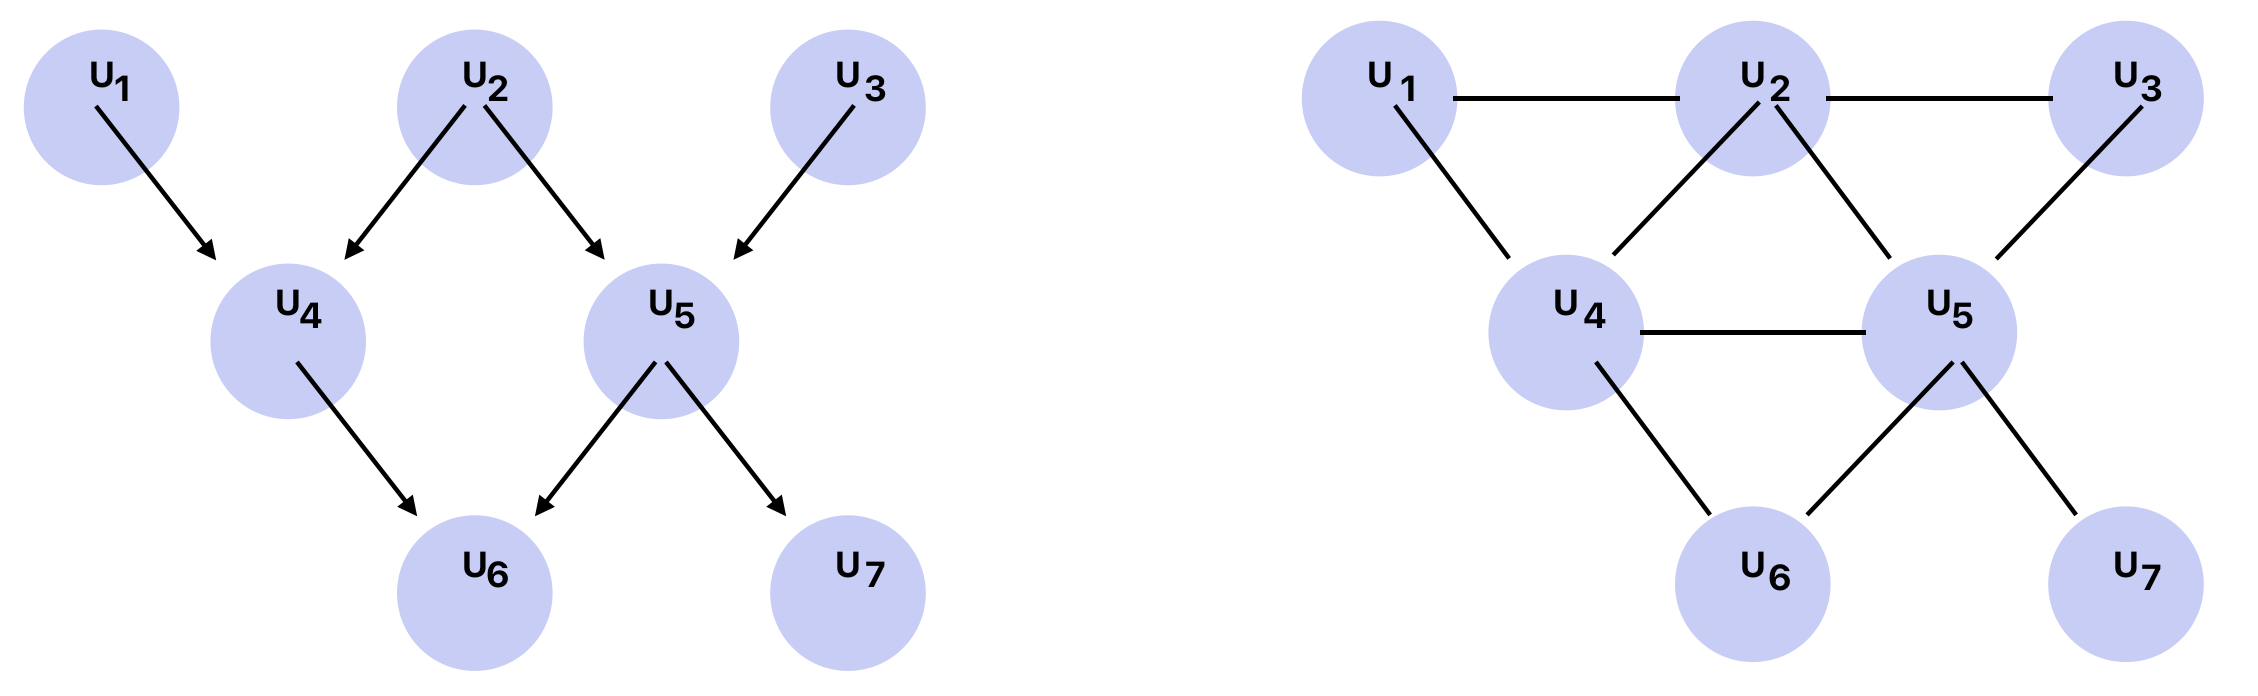
\includegraphics[width=1\linewidth]{Figures/GMRF Sparrows.png}
    \caption[Illustration of a pedigree as a GMRF]{Illustration of a pedigree as a GMRF, figure and figure text inspired by Figure 1 in \citet{Stensland_GMRF_bayes_animal_model}. On the left, a pedigree structure is depicted as a directed acyclic graph (DAG), where birds $U_1$ and $U_2$ are the parents of bird $U_4$, birds $U_2$ and $U_3$ the parents of bird $U_5$, and birds $U_4$ and $U_5$ the parents of bird $U_6$. Bird $U_7$ has one known parent in $U_5$, and one unknown. On the right, the conditional independence graph of the pedigree structure is given, where the parents sharing offspring is assigned an edge and the direction is removed.}
    \label{fig:GMRF_animal_model}
\end{figure}

% \subsection{Single and Multitrait Animal Model}
% When modelling the observed phenotypic trait values of individuals in a population, caution must be made when modelling the genetic component of the trait using INLA.
% If only one trait is considered, 
% The breeding values $\boldsymbol{\alpha}$ of an individual represents the genetic component of an observed phenotypic trait. 
% FINSIH THIS PART



% Would it be correct to interpret this as meaning that all the covariance is explained by relatedness, and that the additive variance is a scalar? Or is there a more complex covariance structure that might be present?

% \cleardoublepage

\chapter{Theory}
\label{ch:theory}
% The sections on linear regression and linear mixed models are similar to those presented in the authors project thesis \citep{Arnstad:Relative_variable_importance_in_Bayesian_linear_mixed_models:2024}, which lead up to the masters thesis.
\section{Linear regression}
\label{sec:linreg}
All regression models are based on the assumption that the response variable is influenced by one or more covariates (regressors).
The relationship between the response and the covariate is assumed not to be deterministic, so we expect our modelling of the response to be influenced by some random error \citep{GLMM_book}.
This means that the response is treated as a random variable, and it is desirable to decompose the response into systematic components and random components. Throughout this section, we will mostly follow the derivations of \citet{GLMM_book} and \citet{GLMM_book_old}.
\subsection{Linear regression}
\label{sec:simple_linreg}
Assuming that an observed response $y_i$ has a linear relationship with a covariate $x_i$ is the basis for the simple linear regression.
This can be modelled by the equation
\begin{equation}
    y_i = \beta_0 + \beta_1x_i + \varepsilon_i \ ,
\end{equation}
where $\beta_0$ is the intercept, $\beta_1$ is the slope, and $\varepsilon_i$ is the error term.
The error term, or residual, is assumed to be normally distributed with mean zero and variance $\sigma^2$, \textit{i.e.} $\varepsilon_i \sim \mathcal{N}(0, \sigma^2)$.
Generalizing to multiple covariates is straightforward by defining the $n\times p$ matrix $\mathbf{X}$ as a design matrix with, including an intercept, the $p$ covariates in the columns and the $n$ observations in the rows.
With this definition, the linear regression model can be written as
\begin{equation}
    \label{eq:linreg}
    \mathbf{y} = \mathbf{X}\boldsymbol{\beta} + \mathbf{\varepsilon} \ ,
\end{equation}
where now $\mathbf{y}=(y_1, y_2, ..., y_n)$ is a vector of $n$ responses, $\boldsymbol{\beta}=(\beta_0, \beta_1, ..., \beta_{p-1})$ is a vector of coefficients including the intercept $\beta_0$, and $\mathbf{\varepsilon}=(\varepsilon_1, \varepsilon_2, ..., \varepsilon_n)$ is a vector of error terms.
The error terms are assumed to be independent and identically distributed (i.i.d.) with $\boldsymbol{\varepsilon} \sim \mathcal{N}(0, \sigma^2 \mathbf{I})$, where $\mathbf{I}$ is the identity matrix of size $n \times n$.
Consequently, the response $\mathbf{y}$ is conditionally independent given the covariates $\mathbf{X}$, \textit{i.e.}
\begin{equation}
    \mathbf{y} \lvert \mathbf{X} \sim \mathcal{N}_n(\mathbf{X}\boldsymbol{\beta}, \sigma^2\mathbf{I}) \ .
\end{equation}
In practice, the coefficients $\boldsymbol{\beta}$ are estimated from the maximum likelihood estimation (MLE) method, given by
\begin{equation}
    \label{eq:beta_hat}
    \hat{\boldsymbol{\beta}} = (\mathbf{X}^T\mathbf{X})^{-1}\mathbf{X}^T\mathbf{y} \ .
\end{equation}

\subsection{Qualitative covariates}
\label{sec:qualitative}
In many cases the covariates are qualitative, meaning they are categorical variables that can be grouped into different levels or factors.
Qualitative covariates, unlike quantitative, cannot be measured numerically, and we must adjust our modelling to account for this.
A common approach to model qualitative data is to include dummy variables, which are assigned a value $1$ if the observation is in the respective category(factor) and $0$ otherwise.
Given $N$ factors, it is standard practice to model $N-1$ dummy variables and let one factor be captured by the intercept to uniquely determine the model.
Dummy encoding in this way retains the properties of the linear regression, and is limited by the same assumptions.
The model for the response $y_i$, assuming no quantitative covariates, from group $j$ with dummy encoding is then given by
\begin{equation}
    y_i =  \beta_0 + \sum_{j=1}^{N-1} \beta_j x_{i,j} + \varepsilon_i \ ,
\end{equation}
where $\beta_j$ denotes the factor coefficient of observation $i$ and the dummy variable
\begin{equation}
    x_{i,j} = \begin{cases}
        1 & \text{if observation $i$ is in group $j$} \\
        0 & \text{otherwise}
    \end{cases} \ .
\end{equation}
This way of modelling qualitative covariates is intuitive and easy to interpret, but it also assumes that factor specific effects are uniform and fixed across all levels and becomes cumbersome with many categorical covariates. 

\subsection{Correlation among covariates in linear regression}
\label{sec:corr_linreg}
Correlation among covariates is to be expected, as it is natural in many practical applications. However, if the correlation is very strong, this poses some serious problems when interpreting the linear regression model.
The covariates $\mathbf{x}_i$ in a linear regression are assumed to be linearly independent, so that the design matrix $\mathbf{X}$ has full rank.
If the design matrix is not of full rank, that is one or more covariates are perfectly correlated, the model \eqref{eq:linreg} is said to be \textit{multicollinear} \citep{Poole_OFarrell_1971}. 
From \eqref{eq:beta_hat} one can see that if the matrix $\mathbf{X}$ is not of full rank, the term $(\mathbf{X}^T\mathbf{X})^{-1}$ is not invertible and the MLE of $\boldsymbol{\beta}$ does not exist. 
Further, the variance of the MLE of $\boldsymbol{\beta}$ grows as the correlation between covariates grows \citep[p. 116]{GLMM_book}. A larger variance in $\boldsymbol{\hat{\beta}}$ also leads to larger standard errors for $\boldsymbol{\hat{\beta}}$, making it hard to assess the model.
Both coefficients and covariates affect the total marginal model variance, which can be decomposed as
\begin{equation}
    \label{eq:var_y}
    \text{Var}(\mathbf{y}) = \text{Var}(\mathbf{X}\boldsymbol{\beta}) + \text{Var}(\boldsymbol{\varepsilon}) = \boldsymbol{\beta}^T\mathbf{V}\boldsymbol{\beta} + \sigma^2_{\varepsilon} = \sum_{j=1}^p\beta_j^2v_j +\sum_{j=1}^{p-1}\sum_{k=j+1}^{p} \beta_j\beta_k\sqrt{v_jv_k}\rho_{jk} + \sigma_{\varepsilon}^2 \ ,
\end{equation}
where $\mathbf{V} = \text{Cov}(\mathbf{X})$ is the $p \times p$ covariance matrix of the covariates which is assumed to be positive definite, $\boldsymbol{\beta}$ is the $p \times 1$ vector of regression coefficients, $v_j$ the regressor variances for $j=1, ..., p$ found along the diagonal of $\mathbf{V}$ and $\rho_{jk}$ the inter-regressor correlations between regressor $j$ and $k$ \citep{gromping_relaimpo}.
The middle term in \eqref{eq:var_y} consists of the covariance between the covariates and the variance contribution from a single covariate is not immediately clear.

%this term makes it hard to assess the relative importance of each covariate. 
%To assign each covariate with an importance, we need to consider relative importance measures that can handle the correlation among covariates.

%\subsection{Relative variable importance \protect\footnote{This subsection is slightly modified from the project thesis \citep{Arnstad:Relative_variable_importance_in_Bayesian_linear_mixed_models:2024}.}} 
\section{Variable importance in linear regression models}
\label{sec:rel_imp_linreg}
In a regression setting with multiple regression coefficients, it is often desirable to be able to assign each covariate with a measure of its relative importance with respect to the model.
The relative importance of covariate $\mathbf{x}_i$ is defined as the standardised contribution to explained variance in the response $\mathbf{y}$ from $\mathbf{x}_i$ \citep{gromping_relaimpo}.
Assigning relative importance is no trivial task, as correlation among covariates poses a challenge in assessing the relative importance of each covariate.
\newline
\newline



\subsection{Relative importance measures}
\label{sec:rel_imp}
The coefficient of determination, $R^2$, is a widely used and intuitive summary statistic of goodness-of-fit, which can also be used for model comparison. 
Conceptually, the $R^2 \in [0, 1]$ and quantifies the proportion of variance in the response variable that can be attributed to the covariates in the model. 
For the linear regression model, the $R^2$ is defined as
\begin{equation}
    \label{eq:R2}
    R^2 = 1 - \frac{(\mathbf{y}-\mathbf{X}\boldsymbol{\beta})^T(\mathbf{y}-\mathbf{X}\boldsymbol{\beta})}{(\mathbf{y}-\overline{\mathbf{y}})^T(\mathbf{y}-\overline{\mathbf{y}})} = \frac{\text{Var}(\mathbf{y}) - \sigma^2_{\varepsilon}}{\text{Var}(\mathbf{y})} \ ,
\end{equation}
where $\overline{\mathbf{y}}$ is the mean vector of responses $\mathbf{y}$ and $\sigma^2_{\varepsilon}$ denotes the residual variance. 
Instead of referring to the $R^2$ value alone, going forward this thesis will focus on decomposing of the $R^2$ value and allocate a proportion of $R^2$ to the model covariates. 
This decomposition is done in order to assess the relative importance, or variance explained, of each covariate in the model.
% Generally, the variance of a linear regression model can be stated as in equation \eqref{eq:var_y}, however in the case of 
The special case of uncorrelated covariates in \eqref{eq:var_y} gives 
% we obtain  
\begin{equation}
    \label{eq:var_y_uncorrelated}
    \text{Var}(\mathbf{y}) = \sum_{j=1}^p\beta_j^2v_j + \sigma_{\varepsilon}^2 \ ,
\end{equation}
% This case
% , the $R^2$ is consistent with the proportion of variance explained in the response total variance of the response variable \citep{gromping_relaimpo}. 
% This consistency 
and provides a natural decomposition of the $R^2$ in terms of contribution from each covariate, as each predictor $\mathbf{x}_i$ contributes $\beta_i^2v_i$ to the total response variance \citep{gromping_relaimpo}.
In \eqref{eq:var_y} however, the response variance is split into three parts, the first two sums which comes from the regressors and the latter term which is the variance of the error. 
As mentioned, it is the middle term that poses the problem of assigning importance to each covariate, since it is not immediately clear how to distribute the total response variance to each covariate, as some variance contributions in the response variance are shared among covariates. The literature has established some criteria that relative importance measures should fulfill, so that they can be interpreted and compared in a sensible manner \citep{gromping_relaimpo}. As listed in \citet{gromping_relaimpo}, the methods should yield
\begin{enumerate}
    \label{list:criteria}
    \item \textbf{Proper decomposition}: The model variance should be decomposed into shares for each regressor that sum up to the total variance, and the method shall allocate the shares to each regressor.
    \item \textbf{Non-negativity}: Each share of the variance should be non-negative.
    \item \textbf{Exclusion}: If a regressor is excluded from the model, $\beta_j=0$, its share of the variance should be zero.
    \item \textbf{Inclusion}: If a regressor is included in the model, $\beta_j \neq 0$, its share of the variance should be positive.
\end{enumerate}
Further, \citet{gromping_relaimpo} introduces some useful notation for considering variable importance, for the explained variance of a subset of regressors $S$ as 
\begin{equation}
    \text{evar}(S) = \text{Var}(\mathbf{y}) - \text{Var}(\mathbf{y} \lvert \mathbf{x}_j, j\in S) \ ,
\end{equation}
and the added explained variance of a subset $M$ to a model that already contains the covariates in $S$ as
\begin{equation}
    \text{svar}(M \lvert S) = \text{evar}(M \cup S) - \text{evar}(S) \ .
\end{equation}

% \begin{equation}
%     \label{eq:var_y_full}
%     \text{Var}(\mathbf{y}) = \sum_{j=1}^p\beta_j^2v_j + \sum_{j=1}^{p-1}\sum_{k=j+1}^{p} \beta_j\beta_k\sqrt{v_jv_k}\rho_{jk} + \sigma_{\varepsilon}^2 \ ,
% \end{equation}
% where $\beta_j$ is the $j$-th regression coefficient, $v_j$ is the variance of the $j$-th covariate, $\rho_{jk}$ is the correlation between the $j$-th and $k$-th covariate and $\sigma_{\varepsilon}^2$ is the variance of the error term.
\subsection{Naive decompositions of \texorpdfstring{$R^2$}{Lg}}
\label{sec:naive_decomp}
To make it clear that some simple decompositions fail the criteria of relative importance measures, we will consider two naive approaches for decomposing the $R^2$. We denote the $R^2$ of a linear regression with regressors $X_1, \dots, X_p$ as $R^2(\{1, \dots, p\})$ and the relative importance of regressor $X_i$ as $\text{RI}(\{i\})$.
\newline
\newline
The first naive method is to fit a model with all regressors $p$, and then fit a model with all regressors excluding regressor $i$. The relative importance of $X_i$ is then the difference $R^2(\{1, \dots, p\}) - R^2(\{1, \dots, p\} \setminus i)$.
To show how this fails the criteria of relative importance measures, an example from \citet{matre} is discussed. The example considers the simple case 
\begin{equation}
    Y=X_1+X_2, \quad \text{Var}(X_1) = \text{Var}(X_2)=1, \quad \text{Cov}(X_1, X_2)=0.9 \ .
\end{equation}
The $R^2$ of the model with both covariates is $R^2(\{1, 2\})=1$, since the covariates $X_1, X_2$ explain fully the response $Y$. Then one would expect that the importance of $X_1$ and $X_2$ is $0.5$ each, since they both explain half of the response variance.
Using the proposed decomposition, one would calculate
\begin{equation}
    \text{RI}(\{2\}) = R^2(\{1, 2\}) - R^2(\{1\}) = 1 - \frac{\text{Cov}(Y, X_1)^2}{\text{Var}(Y)\text{Var}(X_1)} = 1- \frac{1.9^2}{3.8} \approx 0.05 \ ,
\end{equation}
where it is used that for the simple linear regression, the $R^2$ is given by the squared correlation coefficient between the response and the regressor.
By symmetry $\text{RI}(\{1\})=\text{RI}(\{2\})$, so the sum of the relative importances is $0.1$. However, the total explained variance of the model is $1$, so this decomposition violates the proper decomposition condition.
This decomposition only assign importances to the regressor based on the information that the regressor does not share with any other regressors. Therefore, it does not take into account the shared information and the importance estimated is too low.
\newline
\newline
Another naive decomposition would be to compare the relative importance of a model with one regressor $i$ to the empty model, \textit{i.e.} the model with no covariates. 
The empty model has an $R^2=0$ and therefore for $X_1$ in the above example we would have
\begin{equation}
    \text{RI}(\{1\}) = R^2(\{1\}) - R^2(\{\emptyset\}) = \frac{\text{Cov}(Y, X_1)^2}{\text{Var}(Y)\text{Var}(X_1)} = \frac{1.9^2}{3.8} \approx 0.95 \ .
\end{equation}
Once more by symmetry we have $\text{RI}(\{2\})=\text{RI}(\{1\})$, so the sum of the relative importances is $1.9$, violating the proper decomposition condition.
In contrast to the first naive approach, this decomposition assigns importances based on the full information contained in the regressor. Therefore, it overestimates the importance of each variable, since the shared information is accounted for twice.
\newline
\newline
As we have seen from these naive approaches, the task of decomposing the $R^2$ value is far from trivial, and calls for more sophisticated methods.

\subsection{The Lindeman, Merenda and Gold(LMG) method}
\label{sec:lmg}
A method that handles correlation among covariates, and is frequently reinvented from different approaches, is the Lindeman, Merenda and Gold (LMG) method \citep{gromping_relaimpo}.
We shall therefore discuss it, as it serves an important role as a leading method for assigning relative variable importance.  
The LMG method takes use of averaging over orders, meaning that it permutes the index set $\{1, ..., p\}$ of the regressors $(p-1)!$ times, excluding the intercept, and sequentially adds the regressors to the model for each permuted index set.
By adding regressors sequentially for each permutation, one can investigate how the importance of the regressors vary depending on what other regressors are included, which is useful when they are correlated.
This is justified by the assumption that there is no relevant ordering of the regressors in the index set \citep{kruskal_lmg_1987}.
For each regressor added, starting with none, it allocates a share of explained variance, or importance, and then adds a new regressor.
The final allocated share to the regressor is the average of the allocated shares to that regressor for all permutations of the set of regressors indices. 
This would mean that two correlated regressors, whose importance share varies depending on which is added first, would receive an averaged importance.
Averaging over orders is a statistical tradition \citep{kruskal_lmg_1987} and gives a robust assessment of each regressor's importance by considering different orderings of how they are added to the model. 
The iterative process for the regressors $\{X_0, X_1, X_2, X_3\}$, where $X_0$ is the intercept, would be
\begin{enumerate}
    \item Considering $\{X_1, X_2, X_3\}$, $X_1$ is added to the model, and the share of explained variance allocated to $X_1$ is $\text{svar}(\{1\} \lvert \emptyset)$. $X_2$ is added and allocated a share of $\text{svar}(\{2\} \lvert \{1\})$, and lastly $X_3$ is added and allocated a share of $\text{svar}(\{3\} \lvert \{1, 2\})$.
    \item Considering $\{X_1, X_3, X_2\}$, $X_1$ is added to the model, and the share of explained variance allocated to $X_1$ is $\text{svar}(\{1\} \lvert \emptyset)$. $X_3$ is added and allocated a share of $\text{svar}(\{3\} \lvert \{1\})$, and lastly $X_2$ is added and allocated a share of $\text{svar}(\{2\} \lvert \{1, 3\})$.
\end{enumerate}
The above iteration is repeated for all 6 possible permutations of orderings among regressors to obtain the final result.
This iterative process gives rise to the general formula for share of explained variance allocated to $X_i$ by the LMG method with $p$ regressors,
\begin{equation}
    \label{eq:LMG}
    \text{LMG}(i) = \frac{1}{p!} \sum_{S \subseteq \{1, ..., p\}\setminus i} n(S)! (p - n(S)-1)! \text{svar}(\{i\} \lvert S) \ ,
\end{equation} 
where $n(S)$ is the number of regressors in $S$ \citep{gromping_relaimpo}.
Equation \eqref{eq:LMG} averages the increase in $R^2$, $\text{svar}(\{X_i\})$, when adding the covariate of interest, $X_i$, over all possible orderings of covariates. 
This mean increase over orderings is assigned as the proportion of $R^2$ explained by $X_i$.
The LMG method fulfills all but the exclusion criteria described previously \citep{gromping_relaimpo}, but \citet{gromping_relaimpo} argues that this \textit{"must be seen as a natural result of model uncertainty"} and therefore that this criterion is not indispensable.
Therefore, we find it also suitable for our purposes to focus on the three other criteria.
The setback of the LMG method is the great computational expense that the permutations require when $p$ is large. The complexity is $2^{p-1}$ summations \citep{gromping_relaimpo}, and therefore, the LMG is not suitable for high dimensional models. 



\subsection{Relative weights method}
\label{sec:relativeweights}
A method that takes advantage of the straightforward decomposition of the variance when the fixed covariates are uncorrelated is the relative weights method \citep{johnson_relative_weights}, which will now be discussed.
\newline
\newline
The relative weights method proposes an alternative to the LMG, which is significantly less computationally expensive. 
Intuitively, the relative weights method projects the design matrix $\mathbf{X}$ of the fixed effects into an orthogonal column space, resulting in a matrix $\mathbf{Z}$ with orthogonal columns.
The matrix $\mathbf{Z}$ is then an approximation of $\mathbf{X}$ and will be used as the design matrix in the regression. Since the columns of the design matrix $\mathbf{Z}$ are orthogonal, each covariate is uncorrelated. 
This allows us to decompose the variance in the straightforward manner as in equation \eqref{eq:var_y_uncorrelated}.
% As is mentioned above, decomposing the variance with uncorrelated predictors is straightforward. To see this, one can with out loss of generalization, standardize the repsonse to have the zero-vector as mean and the identity matrix as variance. Then it is clear that the marginal variance can be found as
% \begin{equation}
%     \text{Var}(\mathbf{y}) = \text{Var}(\mathbf{X}^T\boldsymbol{\beta} + \boldsymbol{\varepsilon}) = \boldsymbol{\beta}^T\text{Var}(X)\boldsymbol{\beta} + \sigma^2 = \boldsymbol{\beta}^T\boldsymbol{\beta} + \sigma^2 \ ,
% \end{equation}
% so for each predictor the contribution to the full explained variance is the corresponding regression coefficient squared. This property lies the foundation for the relative weights method, which will now be considered.
\newline
\newline
In relative weights one uses the singular value decomposition \citep{relative_weights_nimon_oswald}, to project the real-valued design matrix $\mathbf{X}$ into an orthonormal matrix $\mathbf{U} \in \mathbb{R}^{n \times n}$ containing the eigenvectors of $\mathbf{X}\mathbf{X}^T$, an $n\times p$ diagonal matrix $\mathbf{D}$ containing the singular values of $\mathbf{X}$ and another orthonormal matrix $\mathbf{V} \in \mathbb{R}^{p \times p}$ containing the eigenvectors of $\mathbf{X}^T\mathbf{X}$ such that
%The above matrix relations differ from Matre, double check them!
\begin{equation}
    \label{eq:SVD}
    \mathbf{X} = \mathbf{UDV^T} \ .
\end{equation}
From the Eckhart-Young-Mirsky theorem \citep{mirsky-theorem} and following the derivations of \citet{johnson_minimization_trace}, one can state that the matrix $\mathbf{X}$, of rank $r$, can be approximated by a matrix $\mathbf{Z} = \mathbf{U}\mathbf{V}^T$ of rank $k\leq r$ such that the difference under the squared Frobenius norm
\begin{equation}
    \lVert \mathbf{X} - \mathbf{Z} \rVert_F^2 = tr \left( (\mathbf{X} - \mathbf{Z})^T(\mathbf{X} - \mathbf{Z}) \right) \ ,
\end{equation}
is minimized. The relative weights approximation now utilizes the matrix $\frac{1}{\sqrt{n-1}}\mathbf{{Z}}$ \citep{johnson_relative_weights}, where the factor $\frac{1}{\sqrt{n-1}}$ is the standardisation factor for $\mathbf{Z}$ \citep{matre}, and regresses on $\mathbf{Z}$ to find the MLE $\boldsymbol{\beta_Z}$ as
\begin{equation}
    \begin{aligned}
        \boldsymbol{\beta_Z} & = (\mathbf{Z}^T\mathbf{Z})^{-1}\mathbf{Z}\mathbf{y} \\
        & = \left((n-1) \mathbf{VU}^T\mathbf{UV}^T \right)^{-1} \sqrt{n-1}\mathbf{VU}^T\mathbf{y} \\
        & = \frac{1}{\sqrt{n-1}}\mathbf{V}\mathbf{U}^T\mathbf{y} \ .
    \end{aligned}
\end{equation} 
As $\mathbf{Z}$ is orthogonal, the relative importance for each column $\mathbf{z_i}$ with respect to the response $\mathbf{y}$ can be found as the square of $\beta_{Z, i}^2$. %denoted as $\boldsymbol{\beta_Z}^{[2]}$. 
Once these importances are obtained, \citet{johnson_relative_weights} argues that we should regress $\mathbf{X}$ on $\mathbf{Z}$ to obtain the weights that relate the importance of each column of $\mathbf{Z}$ to each column of $\mathbf{X}$. These weights can be calculated from the matrix
\begin{equation}
    \label{eq:lambda_rw}
    \boldsymbol{\Lambda} = (\mathbf{Z}^T\mathbf{Z})^{-1}\mathbf{Z}^T\mathbf{X} = (\mathbf{V}\mathbf{U}^T\mathbf{U}\mathbf{V}^T)^{-1}\mathbf{V}\mathbf{U}^T\mathbf{U}\mathbf{D}\mathbf{V}^T = \mathbf{V}\mathbf{D}\mathbf{V}^T \ ,
\end{equation}
where $\mathbf{Z}$ is orthogonal. The contribution from a column of $\mathbf{z_i}$ with respect to a column $\mathbf{x}_j$ is given by the squared entry $\boldsymbol{\Lambda}_{ij}^2$, with the squared columns of $\mathbf{\Lambda}$ summing to one and acting as weights.
The contribution from a column $\mathbf{x}_j$ with respect to the response $\mathbf{y}$, \textit{i.e.} the relative importance, is then estimated as the matrix product \citep{johnson_relative_weights}
\begin{equation}
    \label{eq:RI_lambda}
    \text{RI}(\mathbf{X}) = \boldsymbol{\Lambda}^{[2]} \boldsymbol{\beta_Z}^{[2]} \ , 
\end{equation}
with $\text{RI}$ as a column vector where each entry $j$ contains the estimate of the relative importance corresponding to column $j$ of $\mathbf{X}$.
The notation $\boldsymbol{\xi}^{[2]}$ for some $\boldsymbol{\xi}$ represents the Schur product of $\boldsymbol{\xi}$ with itself, \textit{i.e.} element wise squaring of each element in $\boldsymbol{\xi}$.
In \citet[Section 2.5.3]{matre} it is shown that the relative weights method fulfills the same three criteria as the LMG method, because $\mathbf{Z}$ and $\mathbf{X}$ are linear combinations of each other and due to the properties of $\boldsymbol{\Lambda}$.



% \newline
% \newline
% Due to the popularity of $R^2$, it is desirable to also be able to decompose the $R^2$ in the case of correlated covariates, such that it is consistent with the variance of the response.
% In (\ref{eq:var_y_full}) the response variance is split into three parts, the first two sums which comes from the regressors and the latter term which is the variance of the error. 
% It is the middle term that poses the problem of assigning importance to each covariate, since it contains the covariance between the covariates.
% The literature has established some conditions that relative importance measures should fulfill, so that they can be interpreted and compared in a sensible manner \citep{gromping_relaimpo}. As listed in \citet{gromping_relaimpo}, the methods should have
% \begin{enumerate}
%     \label{list:criteria}
%     \item \textbf{Proper decomposition}: The model variance should be decomposed into shares for each regressor that sum up to the total variance, and the method shall allocate the shares to each regressor.
%     \item \textbf{Non-negativity}: Each share of the variance should be non-negative.
%     \item \textbf{Exclusion}: If a regressor is excluded from the model, $\beta_j=0$, its share of the variance should be zero.
%     \item \textbf{Inclusion}: If a regressor is included in the model, $\beta_j \neq 0$, its share of the variance should be positive.
% \end{enumerate}
% Before moving on the such methods, some notation in accordance with \citet{gromping_relaimpo} will be introduced, namely
% \begin{equation}
%     \text{evar}(S) = \text{Var}(Y) - \text{Var}(Y \lvert X_j, j\in S) 
% \end{equation} 
% and
% \begin{equation}
%     \text{svar}(M \lvert S) = \text{evar}(M \cup S) - \text{evar}(S) \ ,
% \end{equation} 
% where $S$ is a subset of regressors, $\text{Var}(Y \lvert X_j, j\in S)$ denotes the variance of $Y$ conditioned on $X_j, j\in S$ being fixed, $\text{evar}(S)$ is the explained variance of the regressors in $S$ and $\text{svar}(M \lvert S)$ is the gain in variance explained by adding regressors from the subset $M$ to the model that already contains the regressors $S$. 

\section{Extensions of the linear regression model}
The linear regression model is a popular tool in many sciences, but it has limitations when one wants to model more complex structures between the response and covariates. We now generalize the concept of linear regression to be able to model more complex data structures.
\subsection{Generalized linear models (GLMs)}
\label{sec:GLM}
The first step in expanding the linear regression model, is to allow the responses to be non-Gaussian. 
%The linear regression and linear mixed model assumes that the response can be modelled as a linear combination of the fixed and random effects which, as we have seen, leads to the conditional distribution of the response being a normal distribution.
Instead of considering only the normal distribution as the distribution of the response, one can consider general responses belonging to the exponential family.
Assume that we have $N$ observations of the response $y_{i}$, where $i=1, ..., N$, that are conditionally independent given the fixed effects.
Then, $y_{i}$ belongs to the univariate exponential family if
\begin{equation}
    \label{eq:exp_family}
    f(y_{i} \lvert \theta_{i}, \phi) = \exp\left(\frac{(y_{i}\theta_{i} - b(\theta_{i}))}{a(\phi)} + c(y, \phi) \right) \ ,
\end{equation}
for some functions $a(\cdot), b(\cdot)$ and $c(\cdot)$, where $\theta_{i}$ is the parameter of the distribution, $\phi$ is a dispersion parameter and $\theta_{i}$ is a canonical parameter if $\phi$ is known \citep{GLMM_book_old}. 
It is required that the function $b(\cdot)$ is twice differentiable, that the density function $f(y_{i} \lvert \theta_{i}, \phi)$ is normalizable and that the support of $f(y_{i} \lvert \theta_{i}, \phi)$ is not dependent on $\theta$.
Two key properties, expectation and variance, of the exponential family are given by
\begin{equation}
    \begin{aligned}
        \mathbb{E}(Y \lvert \theta) &= b'(\theta) \\
        \text{Var}(Y \lvert \theta) &= a(\phi) b''(\theta) \ ,
    \end{aligned}
\end{equation}
where $b''(\theta)$ may also be referred to as the variance function \citep{GLMM_book}, we have left out indexing, and a proof can be found in \Cref{ap:proofs}.
In the canonical form, the parameter $\theta_{i}$ coincides with the linear predictor $\eta_{i}$ defined as 
\begin{equation}
    \theta_{i} = \eta_{i} = \mathbf{x}_{i}^T\boldsymbol{\beta}  \ . %= g(\mathbb{E}(y_{i, j} \lvert \theta_{i, j})) \ ,
\end{equation}
To connect the linear predictor $\eta_{i}$ to the response, we define a monotonic, differentiable link function $g(\cdot)$ such that
\begin{equation}
    \eta_{i} = g(\mu_{i}) = g(\mathbb{E}(y_{i}))\ .
\end{equation} 
For normally distributed responses, one typically uses the identity function as the link function, which yields the linear regression model. If one considers a binary response, the perspective changes. In a binary regression, one wishes to analyse how the covariates influence the probability 
\begin{equation}
    \pi_i = \mathbb{P}(y_i = 1 \lvert \mathbf{x}_i) = \mathbb{E}[y_i] \ .
\end{equation}
This requires that $\mathbb{E}[y_i]$ lies in the interval $[0, 1]$ as it represents a probability measure. Therefore, the inverse of the link function, $h(\eta_i)$ must transform the linear predictor in such a way that the expectation fulfills this criterion \citep{GLMM_book}. A popular choice of inverse link function is the logistic response function 
\begin{equation}
    \pi_i = h(\eta_i) = \frac{\exp(\eta_i)}{1 + \exp(\eta_i)} \ , 
\end{equation} 
yielding the logit-link function
\begin{equation}
    g(\pi_i) = \log\left(\frac{\pi_i}{1-\pi_i}\right) = \eta_i \ ,
\end{equation}
which will be further investigated later on. An intuitive interpretation of the coefficients can be made by noticing that the odds
\begin{equation}
    \frac{\pi_i}{1-\pi_i} = \exp(\eta_i) = \exp(\beta_0)\exp(\beta_1x_{1, i})...\exp(\beta_px_{1, p}) \ ,
\end{equation}
is affected by the covariates in an exponential-multiplicative form \citep{GLMM_book}. Another common regression type is regressing on count data. The most common way of modelling count data is by using the Poisson distribution, which assumes that the events occurring in a time interval or spatial region follow a Poisson process \citep{GLMM_book_old}. The count of how many events $y_i$ that happen in this time interval or region is said to follow a Poisson distribution with some rate $\lambda_i = \mathbb{E}[y_i]$. As the number of events occurring cannot be negative, the rate is also restricted to positive values. The common choice of inverse link function is therefore 
\begin{equation}
    \lambda_i = \exp(\eta_i) = \exp(\beta_0)\exp(\beta_1x_{1, i})...\exp(\beta_px_{1, p}) \ ,
\end{equation} 
which means that the link function is then the logarithm of the rate \citep{GLMM_book}, \textit{i.e.}
\begin{equation}
    \ln (\lambda_i) = \eta_i \ .
\end{equation}


% Some examples of link functions are the identity function for the linear regression, the logit and probit functions for the Bernoulli distribution and the log function for the Poisson distribution.

% Instead of modelling the response as having a linear relationsship with the covariates, one links the expected value of the response, $\mathbb{E}[Y]$ to the linear predictor $\mathbf{X}\boldsymbol{\beta}$ through a link function $g(\cdot)$. 




\subsection{Linear mixed models (LMMs)}
\label{sec:LMM}
Data often comes in clustered form, for example due to repeated measurements of the covariate over time. 
Clustered data violate with the assumption of independent responses in linear regression and must be properly accounted for. One solution to this is to introduce random effects that are cluster specific, but independent of the fixed effects and the other clusters. Let the population contain $m$ underlying clusters, with $n_j, j=1, ..., m$ observations in each cluster, so that $\mathbf{y} \in \mathbb{R}^{(N \times 1)}$ where $N = \sum_{j=1}^m n_j $. Assume that we investigate $q$ random effects, including a random intercept and $q-1$ random slopes, such that the random effects vector can be written as 
\begin{equation}
    \label{eq:alpha}
    \boldsymbol{\alpha} = (\boldsymbol{\alpha}_1, ..., \boldsymbol{\alpha}_{m})^T \ ,
\end{equation}
where each $\boldsymbol{\alpha}_j \in \mathbb{R}^{q \times 1}$ is assumed independent and represents the random effects for cluster $j$ and has length $q$. For a cluster $j$ the vector $\boldsymbol{\alpha}_j \sim \mathcal{N}_q(\mathbf{0}, \mathbf{\Sigma})=\mathcal{N}_q(\mathbf{0}, \mathbf{Q}^{-1})$ where $\mathbf{\Sigma}$ is the $q \times q$ unknown covariance for the random effects assumed to be positive definite and $\mathbf{Q} = \mathbf{\Sigma}^{-1}$ the corresponding precision matrix. 
If the random effects for each cluster are independent of each other, the covariance matrix $\mathbf{\Sigma} = \text{diag}(\sigma_0^2, ..., \sigma_q^2)$.
The linear mixed model now takes the form
\begin{equation} 
    \label{eq:LMM}
    \mathbf{y} = \mathbf{X}\boldsymbol{\beta} + \mathbf{U}\boldsymbol{\alpha} + \boldsymbol{\varepsilon} \ ,
\end{equation}
where $\mathbf{X} \in \mathbb{R}^{N \times p}$ is the design matrix for the fixed effects, $\boldsymbol{\beta} \in \mathbb{R}^{p \times 1}$ are the regression coefficients for the fixed effects, $\mathbf{U} = \text{diag}(\mathbf{U_j}) \in \mathbb{R}^{N \times q}$ is the design matrix for the random effects and $\mathbf{U}_j \in \mathbb{R}^{n_j \times q}$ is the design matrix for cluster $j$. 
Since $\boldsymbol{\alpha}$ is a random variable with zero expectation, the parameters to estimate are the variance of each random effect $\mathbf{\Sigma}_{kk}=\sigma_k^2$ and their covariance $\mathbf{\Sigma}_{k, l} = \sigma_{k, l}$, where $k, l =1, ..., q$.
In practice, it is often easier to estimate the precision rather than the variance, so calculations often involve the precision matrix $\mathbf{Q}$ rather than the covariance matrix $\mathbf{\Sigma}$.
In this model the independence between clusters are conserved for the response as a whole, but it expresses the correlation that observations of the same cluster have through the random effects.
As for the simple linear regression it is assumed that $\mathbf{X}\boldsymbol{\beta}$ is fixed, and that $\mathbf{U}$ is given, so they do not contribute to the model's variance. Therefore, the conditional expectation $\mathbb{E}(\mathbf{y} \lvert \mathbf{X}, \mathbf{U}) = \mathbf{X}\boldsymbol{\beta}$ is easily obtained, and the conditional variance can be calculated as
\begin{equation} \label{eq:cond_var_LMM}
    \text{Var}(\mathbf{y} \lvert \mathbf{X}, \mathbf{U}) = \text{Var}(\mathbf{X}\boldsymbol{\beta}  + \mathbf{U}\boldsymbol{\alpha} + \boldsymbol{\varepsilon}) = \mathbf{U}\text{Var}(\boldsymbol{\alpha})\mathbf{U}^T + \sigma^2\mathbf{I} = \mathbf{U}\mathbf{G}\mathbf{U}^T + \sigma^2\mathbf{I} \ ,
\end{equation}
where $\mathbf{I}\in \mathbb{R}^{N\times N}$ and $\mathbf{G} \in \mathbb{R}^{mq \times mq}$ is the block diagonal covariance matrix of the random effects, with $\mathbf{\Sigma}_j$ along the diagonal for $j=1, ..., m$. 
As we assume that the random effects are independent of the fixed effects, and that the random error term is i.i.d. for each observation, the conditional distribution of $\mathbf{y}$ follows that of a sum of independent normal distributions, \textit{i.e.}
\begin{equation}
    \mathbf{y} \lvert \mathbf{X}, \mathbf{U} \sim \mathcal{N}_n(\mathbf{X}\boldsymbol{\beta}, \mathbf{U}\mathbf{G}\mathbf{U}^T + \sigma^2\mathbf{I}) \ .
\end{equation}

\subsection{Generalized linear mixed models(GLMMs)}
\label{sec:GLMM}
Now that we have expanded the linear regression in two different ways, the final step to complete the regression framework is to combine the LMM and GLM to obtain the GLMM. This is done by adding random effects to the linear predictor, such that
\begin{equation}
    \theta_{i, j} = \eta_{i, j} = \mathbf{x}_{i, j}^T\boldsymbol{\beta} + \mathbf{u}_{i, j}^T \boldsymbol{\alpha}_j \ , %= g(\mathbb{E}(y_{i, j} \lvert \theta_{i, j})) \ ,
\end{equation}
where $j =1, ..., m$ denotes the cluster and $i=1, ..., n_j$ denotes observation $i$ in cluster $j$, $\mathbf{x}_{i, j}$ and $\mathbf{u}_{i, j}$ are the $i$-th columns of the submatrices $\mathbf{X}_{j}$ and $\mathbf{U}_{j}$ of the larger design matrices $\mathbf{X}$ and $\mathbf{U}$ respectively, for cluster $j$.
The assumption of conditional independent observations $y_{i, j}$ is now conditional on the random effect as well as the covariates, and the conditional distribution of $y_{i, j}$ is still assumed to belong to the exponential family. The conditioning on the random effects is also present when choosing the appropriate link function, since one must now, in general, relate $\mathbb{E}[y_{i, j} \lvert \mathbf{x}_{i, j}, \mathbf{u}_{i, j}, \boldsymbol{\alpha}_{j}]$ to the linear predictor $\eta_{i, j}$ \citep{GLMM_book}. For the binary regression, this now means that the link function takes the form 
\begin{equation}
    \ln \left(\frac{\pi_{i, j}}{1- \pi_{i, j}}\right) = \ln \left(\frac{\mathbb{P}(y_{i, j} = 1 \lvert \mathbf{x}_{i, j}, \mathbf{u}_{i, j}, \boldsymbol{\alpha}_{j})}{\mathbb{P}(y_{i, j} = 0 \lvert \mathbf{x}_{i, j}, \mathbf{u}_{i, j}, \boldsymbol{\alpha}_{j})}\right) = \eta_{i, j}  \ ,
\end{equation}
and for regression on count responses we have $y_{i, j}$ following a Poisson distribution conditional on $\mathbf{x}_{i, j}, \mathbf{u}_{i, j}$ and $\boldsymbol{\alpha}_j$ with the link function
\begin{equation}
    \ln(\lambda_{i, j}) = \mathbf{x}_{i, j}^T\boldsymbol{\beta} + \mathbf{u}_{i, j}^T \boldsymbol{\alpha}_j \ , = \eta_{i, j} \ .
\end{equation}
For the Poisson random intercept model with log-link however, it is possible to define the model without conditioning on the random effects, if each cluster has only one observation \citep{GLMM_book}. This is done by noting that
\begin{equation}
    \lambda_j = \exp(\mathbf{x}_j\boldsymbol{\beta} + \alpha_{0, j}) \ ,
\end{equation}
where $\alpha_{0, j} \sim \mathcal{N}(0, \tau_0^2)$, has a log-normal distribution. This is a special case, in which the marginal model can be determined analytically. In general however, the marginal model is not analytically tractable and so obtaining statistical inference on the GLMMs become increasingly complex when compared to the LMM. Parameter estimation therefore calls for numerical methods such as iterated reweighted least squares in the likelihood framework, or Markov chain Monte Carlo (MCMC) methods in the Bayesian framework, to obtain inference.

% When estimating parameters in a GLMM, the joint distribution of the observations is not generally tractable. Therefore, parameter estimation requires more sophisticated methods in both the likelihood and Bayesian framework.

% The linear mixed model can be generalized to include more complex relationships between the response and the covariates. 
% As seen, both for the linear regression and linear mixed model, the response is assumed to have a linear relationship with covariates, leading to a conditional normal distribution of the response.
% %The linear regression and linear mixed model assumes that the response can be modelled as a linear combination of the fixed and random effects which, as we have seen, leads to the conditional distribution of the response being a normal distribution.
% Instead of considering only the normal distribution as the distribution of the response, one can consider general responses belonging to the exponential family.
% Assume that each response $y_{i, j}$, where $j =1, ..., m$ denotes the cluster and $i=1, ..., n_j$ denotes the observations in cluster $j$, are conditionally independent given the fixed and random effects.
% Then, $y_{i, j}$ belongs to the univariate exponential family if
% \begin{equation}
%     \label{eq:exp_family}
%     f(y_{i, j} \lvert \theta_{i, j}, \phi) = \exp\left(\frac{(y_{i, j}\theta_{i, j} - b(\theta_{i, j}))}{a(\phi)} + c(y, \phi) \right) \ ,
% \end{equation}
% for some functions $a(\cdot), b(\cdot)$ and $c(\cdot)$, where $\theta_{i, j}$ is the parameter of the distribution, $\phi$ is a dispersion parameter and $\theta_{i, j}$ is a canonical parameter if $\phi$ is known \citep{GLMM_book_old}. 
% It is required that the function $b(\cdot)$ is twice differentiable, that the density function $f(y_{i, j} \lvert \theta_{i, j}, \phi)$ is normalizable and that the support of $f(y_{i, j} \lvert \theta_{i, j}, \phi)$ is not dependent on $\theta$.
% Two key properties, expectation and variance, of the exponential family are given by
% \begin{equation}
%     \begin{aligned}
%         \mathbb{E}(Y \lvert \theta) &= b'(\theta) \\
%         \text{Var}(Y \lvert \theta) &= a(\phi) b''(\theta) \ ,
%     \end{aligned}
% \end{equation}
% where $b''(\theta)$ may also be refered to as the variance function \citep{GLMM_book} we have left out indexing, and a proof can be found in \Cref{ap:proofs}.
% In the canonical form, the parameter $\theta_{i, j}$ coincides with the linear predictor $\eta_{i, j}$ defined as
% \begin{equation}
%     \theta_{i, j} = \eta_{i, j} = \mathbf{x}_{i, j}^T\boldsymbol{\beta} + \mathbf{u}_{i, j}^T \boldsymbol{\alpha}_j %= g(\mathbb{E}(y_{i, j} \lvert \theta_{i, j})) \ ,
% \end{equation}
% where $\mathbf{x}_{i, j}$ and $\mathbf{u}_{i, j}$ are the $i$-th columns of the submatrices $\mathbf{X}_{j}$ and $\mathbf{U}_{j}$ of the larger design matrices $\mathbf{X}$ and $\mathbf{U}$ respectively, for cluster $j$. If the model contains only fixed effects, it is referred to as a generalized linear model (GLM) and if contains both fixed and random effects it is called a generalized linear mixed model (GLMM).
% To connect the linear predictor $\eta_{i, j}$ to the response, we define a monotonic, differentiable link function $g(\cdot)$ such that
% \begin{equation}
%     \eta_{i, j} = g(\mu_{i, j}) = g(\mathbb{E}(Y_{i, j}))\ .
% \end{equation} 
% Some examples of link functions are the identity function for the LMM, the logit and probit functions for the Bernoulli distribution and the log function for the Poisson distribution.









\section{Extending \texorpdfstring{$R^2$}{Lg} to GLMMs}
\label{sec:R2_GLMM}
As we generalized the linear regression to LMMs, GLMs and GLMMs, we have to find a generalization of the concept of $R^2$ in order to generalize the concept of variable importance. This is fundamental to be able to propose a method for decomposing the $R^2$ and thereby assigning relative importance to covariates.
However, the task of determining the $R^2$, and decomposing it, is not a trivial task in the linear regression case and becomes even more complex in the case of GLMMs.
Many extensions have been proposed, but due to a variety of theoretical problems and/or computational difficulties, no consensus has been reached on a framework for calculating the $R^2$ for GLMMs \citep{nakagawa2013general}.
To get an overview of the status quo for $R^2$, we will follow the paper by \citet{nakagawa2013general} and go through the different components added to the linear regression to compose the GLMMs.
\subsection{\texorpdfstring{$R^2$}{Lg} for GLMs}
Recalling the definition of the $R^2$ from \eqref{eq:R2}, we now generalize this to the GLMs. This topic has been subject to significant research, \citep{maddala1983limited, cameron1997r, menard2000coefficients, nakagawa2013general} and has evolved through various methodologies. The methods first suggested was based on the likelihood function of the model to be analysed. We will not implement such methods, as they are not suitable for the full generalization to be made later on, however they are important in building a framework for the $R^2$ value and are therefore included.
To illustrate the likelihood based generalization of the $R^2$ value to GLMs, consider the (scaled) deviance $\mathcal{D}(\mathbf{y}\lvert \theta)$ function which is defined as twice the difference between the log-likelihood of the \textbf{saturated model} and the log-likelihood of the model of interest \citep{GLMM_book_old}.
The saturated model denotes the model of the maximum achievable log-likelihood, and therefore fits the data perfectly. 
For a linear regression, with $\theta=(\boldsymbol{\beta}, \sigma^2)$, we would therefore obtain
\begin{equation}
    \begin{aligned}
    \mathcal{D}(\mathbf{y}\lvert \hat{\theta}) &= -2\left( \ln(\mathcal{L}(\boldsymbol{\beta}, \sigma^2 \lvert \mathbf{y})) - \ln(\mathcal{\hat{L}}(\boldsymbol{\hat{\beta}}, \hat{\sigma^2} \lvert \mathbf{y}))  \right) = -2\left( l(\boldsymbol{\beta}, \sigma^2 \lvert \mathbf{y}) - l(\boldsymbol{\hat{\beta}}, \hat{\sigma^2} \lvert \mathbf{y})  \right) \\
    & = -2\left(-\frac{n}{2}\ln(2\pi\sigma^2) - \frac{1}{2\sigma^2} (\mathbf{y}-\mathbf{X}\boldsymbol{\beta})^T(\mathbf{y}-\mathbf{X}\boldsymbol{\beta}) + \frac{n}{2}\ln(2\pi\sigma^2)  \right) \\
    & = \frac{1}{\sigma^2} (\mathbf{y}-\mathbf{X}\boldsymbol{\beta})^T(\mathbf{y}-\mathbf{X}\boldsymbol{\beta}) %\\
    %& = 1-R^2 \ ,
    \end{aligned}
\end{equation}
where $\mathcal{\hat{L}}$ denotes the saturated model.
Optimally, it is desirable to have as small deviance as possible while at the same time having a model that is not too complex.
The best practice of the deviance is not as model fit, but rather model comparison, where one compares models through the reduction in deviance \citep{GLMM_book_old}.
Since the model of interest is nested within the saturated model, the deviance coincides with the likelihood ratio test. 
By comparing the model of interest to the \textbf{null model}, which sets $\mathbf{X}\boldsymbol{\beta}=\mathbf{\overline{y}}$, one obtains for the linear regression
\begin{equation}
    \begin{aligned}
        \frac{\mathcal{D}(\mathbf{y}\lvert \hat{\theta})}{\mathcal{D}(\mathbf{y}\lvert \theta_0)}
        &= \frac{\frac{1}{\sigma^2} (\mathbf{y}-\mathbf{X}\boldsymbol{\beta})^T(\mathbf{y}-\mathbf{X}\boldsymbol{\beta})}{\frac{1}{\sigma^2} (\mathbf{y}-\mathbf{\overline{y}})^T(\mathbf{y}-\mathbf{\overline{y}})} = 1 - R^2
    \end{aligned}
\end{equation}
This is the foundation for the definitions of the generalization of $R^2$ to GLMs \citep{nakagawa2013general}, which primarily rely on a ratio of the maximum likelihood of the model of interest and null model.
In \citet{nakagawa2013general}, two different, likelihood based, $R^2$ measures are given as
\begin{equation}
    R^2_G = \left[1- \left(\frac{\mathcal{L}_0}{\mathcal{L}_M}\right) ^{2/n} \right] \frac{1}{1-(\mathcal{L}_0)^{2/n}}
\end{equation}
and 
\begin{equation}
    R^2_D = 1 - \frac{-2\ln(\mathcal{L}_M)}{-2 \ln(\mathcal{L}_0)}
\end{equation}
where $n$ denotes the total sample size, $\mathcal{L}_0$ is the likelihood of the null model and $\mathcal{L}_M$ is the likelihood of the model of interest.
The reason why we will not apply likelihood based $R^2$ measures is that when generalizing to the larger class of GLMMs, it is often desirable to do parameter estimation using the restricted maximum likelihood (REML) instead of the maximum likelihood (ML) \citep{GLMM_book}.
The REML estimator transforms the data, meaning that models cannot be compared when fitted, and therefore the proposed measure of $R^2$ is not applicable to the REML framework \citep{nakagawa2013general}.
However, the extension of the $R^2$ measure to the larger class GLMMs will also cover the special case of GLMs, and is discussed further below in \Cref{sec:R2GLMM}.

\subsection{\texorpdfstring{$R^2$}{Lg} for LMMs and random slope models}
\label{sec:R2_LMM}
In the LMMs, as opposed to the linear regression, one wishes to estimate two or more variance components instead of only the residual error variance.
This increases complexity and makes the task of assigning relative importance to the covariates even more challenging.
Initially, a definition was proposed for the $R^2$ in the LMMs that included fixed effects separately and then estimated the reduction in each variance component \citep[refering to Raudenbush \& Bryk 1986, 1992]{nakagawa2013general}. 
This violated a key condition, as adding a covariate could decrease $\sigma^2_{\varepsilon}$ while at the same time increasing $\sigma^2_{\alpha}$, which can lead to a negative $R^2$.
To handle this problem, Snijders \& Bosker (1994) \citep{nakagawa2013general} proposed a new definition of the $R^2$, dividing it into two components $R^2_1$ and $R^2_2$.
Consider the simple random intercept model in scalar form;
\begin{equation}
    \label{eq:random_intercept}
    y_{i, j} = \beta_0 + \beta_1x_{i, j} + \alpha_{j} + \varepsilon_{i, j} \ ,
\end{equation}
where $y_{i, j}$ denotes the $i$th observation in cluster $j$, $\beta_0$ is the fixed intercept, $x_{i, j}$ is the covariate for the $i$th observation in cluster $j$, $\beta$ is the global coefficient of the fixed effect, $\alpha_{j}$ is the random intercept for cluster $j$ and $\varepsilon_{i, j}$ is the residual error for the $i$th observation in cluster $j$. The two $R^2$ components can then be expressed in two ways, with the first being
\begin{equation}
    \begin{aligned}
    R_1^2 &= 1-\frac{\text{Var} (y_{i, j} - \hat{y}_{i, j})}{\text{Var} (y_{i, j})} = 1-\frac{\sigma_{\varepsilon}^2 + \sigma^2_{\alpha}}{\sigma_{\varepsilon 0}^2 + \sigma^2_{\alpha 0}} \\
    \hat{y_{i, j}} &= \beta_0 + \mathbf{x}_{i, j}^T\beta \ ,
    \end{aligned}
\end{equation}
where $\sigma_{\varepsilon 0}^2$ and $\sigma^2_{\alpha 0}$ denote the residual and random effect variances of the null model respectively and $\hat{y}_{i, j}$ denotes the fitted value of observation $i$ in the $j$th cluster \citep{nakagawa2013general}.
Similarly, the second component is defined as
\begin{equation}
    \begin{aligned}
    R_2^2 &= 1-\frac{\text{Var} (y_{j} - \hat{\bar{y_{j}}})}{\text{Var} (\overline{y_{j}})} = 1-\frac{\sigma_{\varepsilon}^2 + \sigma^2_{\alpha}/k}{\sigma_{\varepsilon 0}^2 + \sigma^2_{\alpha 0}/k} \\
    k &= \frac{M}{\sum_{j=1}^M \frac{1}{m_j}} \ ,
    \end{aligned}
\end{equation}
where $\overline{y_j}$ is the mean for each observed value of the $j$th cluster, $\hat{\bar {y_j}}$ is the mean of the fitted values for the $j$th cluster, $k$ is the harmonic mean of the number of observations per cluster, $m_j$ is the number of observations for the $j$th cluster and $M$ is the total number of clusters \citep{nakagawa2013general}. 
Note that we have formulated the above definitions in a notation corresponding to our previous formulation of the LMM, and therefore use clusters in general, whereas \citet{nakagawa2013general} refers to a cluster as being individuals with repeated measurements.
% Litt usikker på om dette blir 100% riktig?
The reason for dividing the $R^2$ into two components, is that intuitively the $R^2_1$ measures the within cluster variance explained and the $R^2_2$ measures the between cluster variance explained \citep{nakagawa2013general}.
However, three problems arise when using this definition of the $R^2$ for LMMs. 
Firstly, the $R^2_1$ and $R^2_2$ can decrease in large models, secondly, $R_1^2$ and $R_2^2$ have not been generalized to more complex LMMs with more than one random effect and lastly, it is not clear how to generalize the $R_1^2$ and $R_2^2$ to GLMMs \citep{nakagawa2013general}.
To overcome these obstacles, \citet{nakagawa2013general} proposes a new formulation of the $R^2$ measure. 
Consider a general random intercept model as defined in \Cref{sec:LMM}, with $q$ random intercepts, as
\begin{equation}
    \mathbf{y} = \mathbf{X}\boldsymbol{\beta} + \mathbf{U}\boldsymbol{\alpha} + \boldsymbol{\varepsilon} \ ,
\end{equation}
with the parameters of interest being $\boldsymbol{\beta}$ and the variance components $\sigma^2_{\varepsilon}$ and $\sigma^2_{r}$ for each of the $r=1, ..., q$ random intercepts.
Then define the variance of the fixed effects as 
\begin{equation}
    \sigma^2_f = \text{Var}(\mathbf{X}\boldsymbol{\beta}) = \boldsymbol{\beta}^T\text{Var}(\mathbf{X})\boldsymbol{\beta} \ ,
\end{equation}
and further define the $R^2$ for the LMM as
\begin{equation}
    R^2_{\text{LMM(m)}} = \frac{\sigma^2_f}{\sigma^2_f + \sum_{r=1}^{q}\sigma^2_{r} + \sigma^2_{\varepsilon}} \ .
\end{equation}
This definition of the $R^2_{\text{LMM}}$ represents the marginal $R^2_{\text{LMM}}$, denoted by $(m)$, as it measures the proportion of the variance explained by the fixed effects alone, whereas the conditional $R^2_\text{LMM}$ can be defined as 
\begin{equation}
    R^2_{\text{LMM(c)}} = \frac{\sigma^2_f + \sum_{r=1}^{q}\sigma^2_{r}}{\sigma^2_f + \sum_{r=1}^{q}\sigma^2_{r} + \sigma^2_{\varepsilon}} \ .
\end{equation}
By inspection, it is clear that this definition will never lead to negative values of the $R^2_{\text{LMM}}$. 
It may occur that the $R^2_{\text{LMM}}$ value may decrease when adding more covariates to the model, although \citet{nakagawa2013general} argues that this is unlikely.
This definition now covers the random intercept model, but has not taken into account the possibility of having a LMM with a random slope. 
To further extend the $R^2$ to the random slope model, \citet{Johnson2014} proposes a method for computing the mean random effect variance.
Consider the simple random intercept and slope model,
\begin{equation}
    y_{i, j} = \beta_0 + \beta_1x_{i, j} + \alpha_{0, j} + \alpha_{1, j}x_{i, j} + \varepsilon_{i, j} \ ,
\end{equation}
where the same notation is used as in \eqref{eq:random_intercept} with $\boldsymbol{\alpha_j}=(\alpha_{0, j}, \alpha_{1, j})$ being the random effect, $\alpha_{0, j}$ denoting the random intercept and $\alpha_{1, j}$ now denoting the random deviation from the global slope $\beta_1$, for cluster $j$.
The general assumption on the random effects are that 
\begin{equation}
    \begin{aligned}
    \begin{pmatrix}
        \alpha_0 \\
        \alpha_{1}
    \end{pmatrix} 
    \sim \mathcal{N}\left( 
    \begin{pmatrix}
        0 \\
        0
    \end{pmatrix} \ ,
    \boldsymbol{\Sigma} =
    \begin{pmatrix}
        \sigma^2_{\alpha_0} & \sigma_{\alpha_0, \alpha_1} \\
        \sigma_{\alpha_0, \alpha_1} & \sigma^2_{\alpha_1}
    \end{pmatrix} \right)  \ ,
    \end{aligned}
\end{equation}
where $\sigma^2_{\alpha_0}$ and $\sigma^2_{\alpha_1}$ are the variances of the random intercept and random slope respectively, and $\sigma_{\alpha_0, \alpha_1}$ is the covariance between the random intercept and random slope.
Thus, we have three variance components of interest ($\frac{q(q+1)}{2}$ for $q$ random effects) to estimate. 
When inspecting the variance of the random part in the model, we see that it has a dependence on the covariates, as illustrated by 
\begin{equation}
    \begin{aligned}
    \text{Var}(\alpha_{0, j} + \alpha_{1, j}x_{i, j}) &= \text{Var}(\alpha_{0, j}) + 2x_{i, j} \text{Cov}(\alpha_{0, j}, \alpha_{1, j}) + x^2_{i, j}\text{Var}(\alpha_{1, j}) \\
    & = \sigma^2_{\alpha_0} + 2x_{i, j}\sigma_{\alpha_0, \alpha_1} + x^2_{i, j}\sigma^2_{\alpha_1} =: \sigma^2_{r, i, j} \ ,
    \end{aligned}
\end{equation}
where we define $\sigma^2_{r, i, j}$ as the variance of the random effect $\boldsymbol{\alpha}$ for observation $i$ in the $j$th cluster. 
The method proposed by \citet{Johnson2014} is to first estimate all the variance components, and then view the specific random effect as a normal mixture distribution of the random intercept and random slope.
This mixture distribution is characterized as having a common mean of zero, and, if all values of the associated covariate $\mathbf{x}_{i, j}$ are unique, having $N$ different variances with $N$ being the total number of observations.
A mixture distribution with constant mean, has a variance which equals the mean of the individual variances in the distribution \citep[citing Behboodian 1970]{Johnson2014}. 
The proposed variance of the random effect $\boldsymbol{\alpha}$, is therefore the mean of the variance components in $\boldsymbol{\alpha}$, \textit{i.e.}
\begin{equation}
    \overline{\sigma^2_{r}} = \frac{1}{N}\sum_{j=1}\sum_{i=1} \left(\sigma^2_{r, i, j} \right) \ .
\end{equation}
This formulation can be generalized in the case of $q$ random effects, where each random effect has an associated design matrix $\mathbf{U_j}$ and covariance matrix $\mathbf{Q}$ as in \Cref{sec:LMM}, so that for each random effect $r$ we have
\begin{equation}
    \overline{\sigma^2_{r}} = \text{Tr}( \mathbf{U_j}\mathbf{Q}\mathbf{U_j}^T), \ \ r=1, ..., q \ .
\end{equation}
To finally obtain the proposed $R^2$ for the general LMM, \citet{Johnson2014} uses this estimate in the definition given by \citet{nakagawa2013general}, to obtain
\begin{equation}
    R^2_{\text{LMM(m)}} = \frac{\sigma^2_f}{\sigma^2_f + \sum_{r=1}^{q}\overline{\sigma^2_{r}} + \sigma^2_{\varepsilon}} \ ,
\end{equation}
and 
\begin{equation}
    R^2_{\text{LMM(c)}} = \frac{\sigma^2_f + \sum_{r=1}^{q}\overline{\sigma^2_{r}}}{\sigma^2_f + \sum_{i=1}^{q}\overline{\sigma^2_{r}} + \sigma^2_{\varepsilon}} \ ,
\end{equation}
as the marginal and conditional $R^2_{\text{LMM}}$ respectively. 
For the random intercept model with $\sigma_{r, i, j}^2 = \sigma^2_r$, this definition corresponds to the definition by \citet{nakagawa2013general} as 
\begin{equation}
    \overline{\sigma^2_{r}} = \frac{1}{N}\sum_{j=1}\sum_{i=1} \left(\sigma^2_{r, i, j} \right) = \sigma^2_{r, i, j}  = \sigma^2_{r} \ .
\end{equation}
The $R^2_{\text{LMM}}$ proposed by Johnson now lets us compute the $R^2$ for general LMMs, however it is argued in \citet{Johnson2014} whether the improved $R^2$ estimate by taking the random slope into account is worth the added complexity and computational cost.

\subsection{\texorpdfstring{$R^2$}{Lg} for GLMMs}
\label{sec:R2GLMM}
The final step towards a complete generalization for the $R^2$ value of regression models is to extend it to the GLMMs. 
When considering non-normal responses, the link function introduces an aspect not yet discussed, which is to define the residual variance.
One can divide the residual variance $\sigma^2_{\varepsilon}$ into three components, namely distribution specific variance, multiplicative dispersion and additive dispersion \citep{nakagawa2013general}.
The distribution specific variance, $\sigma^2_d$, is inherited from the link function used, and formulas for multiple distributions can be found in \citet{nakagawa2017}. 
However, the multiplicative and additive dispersion is modelled to account for the variance present that exceeds the distribution specific variance, \textit{i.e.} overdispersion \citep{NakagawaSchielzeth2010}.
Therefore, one must specify upon implementation on what scale the overdispersion is to be modelled. 
The multiplicative dispersion, denoted by $\omega$, is overdispersion on the response (data) scale and modelled as a distinct parameter of the assumed distribution of the response $\mathbf{y}$ \citep{NakagawaSchielzeth2010}.
Conversely, the additive dispersion, denoted by $e$, is overdispersion on the latent scale and introduced to the model as an additional random effect in the linear predictor \citep{NakagawaSchielzeth2010}.
Defining the residual variance now depends on the choice of dispersion modelling, and is either defined as
\begin{equation}
    \sigma^2_{\varepsilon} = \omega \sigma^2_{d} 
\end{equation}
or 
\begin{equation}
    \sigma^2_{\varepsilon} = \sigma^2_{d} + \sigma^2_{e} \ ,
\end{equation}
for multiplicative and additive dispersion respectively.
With the residual variance defined, the generalization to of the $R^2$ to GLMMs (thereby also the GLMs) follows the same logic as the LMMs, and $R^2_{\text{GLMM (m)}}$ is defined as
\begin{equation}
    \label{eq:R2_GLMM_m_m}
    R^2_{\text{GLMM(m, m)}} = \frac{\sigma^2_f}{\sigma^2_f + \sum_{r=1}^{q}\overline{\sigma^2_{r}} + \sigma^2_{\varepsilon}} = \frac{\sigma^2_f}{\sigma^2_f + \sum_{r=1}^{q}\overline{\sigma^2_{r}} + \omega \sigma^2_{d}}\ ,
\end{equation}
and
\begin{equation}
    \label{eq:R2_GLMM_m_a}
    R^2_{\text{GLMM(m, a)}} = \frac{\sigma^2_f}{\sigma^2_f + \sum_{r=1}^{q}\overline{\sigma^2_{r}} + \sigma^2_{\varepsilon}} = \frac{\sigma^2_f}{\sigma^2_f + \sum_{r=1}^{q}\overline{\sigma^2_{r}} + \sigma^2_{d} + \sigma^2_{e}}\ ,
\end{equation}
where the same notation as before is used and the subscripts $(\cdot, m)$ and $(\cdot, a)$ denote the multiplicative and additive dispersion respectively.
The conditional $R^2_{\text{GLMM}}$ can be defined similarly as,
\begin{equation}
    \label{eq:R2_GLMM_c_m}
    R^2_{\text{GLMM(c, m)}} = \frac{\sigma^2_f + \sum_{r=1}^{q}\overline{\sigma^2_{r}}}{\sigma^2_f + \sum_{r=1}^{q}\overline{\sigma^2_{r}} + \omega \sigma^2_{d}}\ ,
\end{equation}
and
\begin{equation}
    \label{eq:R2_GLMM_c_a}
    R^2_{\text{GLMM(c, a)}} = \frac{\sigma^2_f + \sum_{r=1}^{q}\overline{\sigma^2_{r}}}{\sigma^2_f + \sum_{r=1}^{q}\overline{\sigma^2_{r}} + \sigma^2_{d} + \sigma^2_{e}}\ ,
\end{equation}
completing the generalization. 

\subsection{Extensions of the LMG and relative weights method}
\label{sec:LMG_ext}
Extensions for both the LMG and the relative weights method have been proposed so that they can decompose the $R^2$ proposed by \citet{nakagawa2013general} also for random intercept models \citep{matre}. 
The extended LMG, denoted as the ELMG, method uses the same permutations as described for the regular LMG, and now decomposes the $R^2$ value for the random intercept model.
% This $R^2$ is described in \Cref{sec:R2_LMM} and effectively divides the variance of the response into the variance of the fixed effects, the random effects and the random error.
For this decomposition, the only extension needed for the LMG formula is to include also the random intercepts as model components, which for covariate $i$ gives
\begin{equation}
    \text{LMG}(i) = \frac{1}{(p+q)!} \sum_{\substack{S \subseteq \{1, ..., p \\ p+1, ..., p+q\} \setminus i }} n(S)! ((p+q) - n(S)-1)! \text{svar}(\{i\} \lvert S) \ , 
\end{equation}
where $p$ denotes fixed effects and $q$ denotes random effects \citep{matre}. It is equivalent to the original LMG method \eqref{eq:LMG} except that here the random intercepts are treated as categorical fixed effects, where we do not consider the columns but rather the whole predictor, either completely in the model or not.
\newline
\newline
To create the extended relative weights (ERW) method, \citet{matre} uses the same transformation of data as for the relative weights method to project the covariates into an orthogonal space. 
Then the fixed effects are treated as one separate block, either in the model or not, and then uses the LMG approach to distribute a share of $R^2$ to each random intercept.
The fixed effects will receive a joint share, which is distributed by using the relative weights method.
Since the LMG approach is used for the $q$ random effects and the block of fixed effects, the complexity of the ERW will follow that of the LMG method for $q+1$ covariates.
\newline 
\newline
Both extensions described comes with new considerations \citep[for full details]{matre}, for example that the inclusion criteria now should read \textit{"If a regressor $\beta_j \neq 0$, or a random intercept $\alpha$ with $\sigma^2(\alpha) > 0$, is included in the model then its share of the variance should be positive"}.



%USING LIKELIHOOD R2 VALUES MEANS THAT ONE CANNOT COMPARE MODELS WHEN USING REML, FIND ROOM TO INCLUDE THIS!


%THIS ARTICLE \citet{NakagawaSchielzeth2010} DESCRBIES REPEATABILITY FOR NON-GAUSSIAN DATA, COULD BE USEFUL LATER



\section{The Bayesian framework}
So far, we have introduced statistical concepts without considering the framework in which they are used.
We now expand the theory to consider the Bayesian framework, which is the framework this thesis will be developed in. 
% \subsection{The frequentist framework}
% The traditional framework of statistics is known as the \textit{frequentist} framework, in which the data is considered in two parts $(y, x)$ where $y$ is thought to be an observation of the random variable $Y$ and $x$ is considered stationary covariates \citep{Cox_2006}.
% Typically, one is solely concerned with the distribution of $Y$ conditional on $x$ and uses the covariates $x$ to describe the system in which $Y$ is observed.
% Therefore, a model, or family of models, for the random variable $Y$ must be chosen, giving rise to the probability density function
% \begin{equation}
%     \label{eq:likelihood}
%     f_Y(y \lvert x, \boldsymbol{\theta}) \ ,
% \end{equation}
% where $\boldsymbol{\theta}$ is the unknown parameter vector containing the parameters belonging to the parameter space of the model \citep{Cox_2006}. 
% The parameter $\boldsymbol{\theta}$ defines key properties of the distribution such as expectation, variance and higher moments and are often the focus of the statistical analysis.
% Often, one can partition the model parameters into two parts, $\boldsymbol{\theta}=\psi, \lambda$, where $\psi$ denotes the parameters of interest and $\lambda$ a nuisance parameter \citep{Cox_2006}.
% The parameters are regarded as unknown constants, and the inference one makes is typically statements that specify a hypothetical long run probability of the parameters taking on certain values.
% To illustrate we use an example from \citet{Cox_2006};
% Consider the mean $\bar{Y}$ of a random variable $Y$ assumed to be normally distributed with observations $(y_1, ..., y_n)$, mean $\mu$ and variance $\sigma^2$.
% It can be shown that
% \begin{equation}
%     \label{eq:mean_normal}
%     \mathbb{P}(\bar{Y} > \mu - z \frac{\sigma}{\sqrt{n}}) = 1-c \ ,
% \end{equation}
% where $\Phi$ denotes the cumulative distribution of the standard normal distribution such that $\Phi(z) = 1-c$.
% This can be rearranged to give the statement 
% \begin{equation}
%     \label{eq:mean_normal_rearranged}
%     \mathbb{P}(\mu < \bar{Y} + z \frac{\sigma}{\sqrt{n}}) = 1 - c \ ,
% \end{equation}
% which \textit{can be interpreted as specifying a hypothetical long run of statements about $\mu$ a proportion $1-c$ of which are correct} \citep{Cox_2006}.
% The belief that the long run behaviour of the data can be used as a basis to draw conclusions is a fundamental idea of the frequentist framework.
\subsection{General idea} 
\label{sec:bayes_general}
The Bayesian framework stems from the notorious theorem developed by Thomas Bayes \citep{bayes_1763}, which states that for events $A$ and $B$, with nonzero probability of occurring, we have
\begin{equation}
    \label{eq:bayes_theorem}
    \mathbb{P}(A\lvert B) = \frac{\mathbb{P}(B \cap A)}{\mathbb{P}(B)} = \frac{\mathbb{P}(B\lvert A)\mathbb{P}(A)}{\mathbb{P}(B)} \ .
\end{equation}
This was generalized by Pierre Simon Laplace \citep{laplace1774}, to also apply to distributions of continuous random variables, namely
\begin{equation}
    \label{eq:bayes_theorem_func}
    \pi(\boldsymbol{\theta} \lvert \mathbf{y}) = \frac{\pi(\mathbf{y} \lvert \boldsymbol{\theta})\pi(\boldsymbol{\theta})}{\pi(\mathbf{y})} \ ,
\end{equation}
where $\pi(\boldsymbol{\theta} \lvert \mathbf{y})$ is called the posterior distribution of $\boldsymbol{\theta}$, $\pi(\mathbf{y} \lvert \boldsymbol{\theta})$ is the likelihood, or sampling, distribution of $\mathbf{y}$, $\pi(\boldsymbol{\theta})$ is the prior distribution of the parameters and $\pi(\mathbf{y}) = \int \pi(\mathbf{y} \lvert \boldsymbol{\theta}) \pi(\boldsymbol{\theta}) < \infty$ is the marginal distribution of the data, which is required to be finite in order to have a proper posterior distribution \citep{gelman2015Bayesian}.
In practice, the marginal distribution is often omitted and one only consider the proportionality of \eqref{eq:bayes_theorem_func}, \textit{i.e.}
\begin{equation}
    \label{eq:bayes_theorem_func_prop}
    \pi(\boldsymbol{\theta} \lvert \mathbf{y}) \propto \pi(\mathbf{y} \lvert \boldsymbol{\theta})\pi(\boldsymbol{\theta}) \ .
\end{equation}
In the context of statistical analysis, with $\boldsymbol{\theta}$ being the parameter vector of the family of models for the random variable $Y$ under investigation, $\pi(\boldsymbol{\theta} \lvert \mathbf{y})$ is interpreted as the distribution of the parameters given the data $\mathbf{y}$.
This is the key element that separates the Bayesian framework from the frequentist framework, as the parameters in $\boldsymbol{\theta}$ are now treated as random variables instead of being point estimates. 

\subsection{Prior and posterior distributions}
Generally, a Bayesian model is built by first introducing some prior knowledge through the prior distribution $\pi(\boldsymbol{\theta})$ and supplementing this with the likelihood function $\pi(\mathbf{y} \lvert \boldsymbol{\theta})$.
The prior distribution must be chosen based on the prior knowledge available, and can either be informative, noninformative or weakly informative \citep{gelman2015Bayesian}. 
As a compromise of the information in the prior and the likelihood of the data, the posterior distribution is obtained. 
The resulting posterior will be different from analysis to analysis, but some general relations between the prior and posterior are discussed in \citet{gelman2015Bayesian}.
In particular, it is stated that \textit{"the posterior variance is on average smaller than prior variance by an amount that depends on the variation in posterior means over the distribution of possible data"} \citep{gelman2015Bayesian}.
This further means that if one wishes to reduce the variability in the posterior, the potential for this lies in reducing the variation of possible posterior means.
The posterior distribution will therefore, in general, be a compromise between the prior and the likelihood, which with increasing sampling size will be increasingly influenced by the likelihood \citep{gelman2015Bayesian}.

\subsection{Penalising complexity (PC) priors}
\label{seq:PC_prior}
Prior distributions pose a great feature by allowing for inclusion of prior information, but also a great challenge in that they must be chosen with caution.
As the theory of priors is vast and out of the scope for this thesis, we will be mostly concerned with the penalising complexity priors proposed in \citet{simpson2017penalising}.
In this paper, four main principles are desirable to follow when choosing a prior distribution, namely 
\begin{enumerate}
    \item \textbf{Occam's razor} - If there is no evidence for a complex mode, a base model should be preferred. 
    \item \textbf{Measure of complexity} - The measure of model complexity is defined as $d(f \lvert \lvert g) = \sqrt{2 \text{KLD}(f \lvert \lvert g)}$ where $\text{KLD}(f \lvert \lvert g)$ denotes the Kullback-Leibler divergence \citep[for more information]{simpson2017penalising}.
    \item \textbf{Constant rate penalisation} - The penalisation, \textit{i.e.} the decay of prior mass, grows as the complexity grows, but it is desirable that this growth is constant.
    \item \textbf{User defined scaling} - Assuming that the user has an idea of the magnitude of the parameter of interest, the user should be able to scale the prior accordingly.
\end{enumerate}
The PC priors pose interpretable, applicable priors which are consistent with the above principles, and are therefore a practical choice for the Bayesian framework \citep{simpson2017penalising}. 
Particularly, for the case of a linear mixed model with a Gaussian random effect $\alpha \sim \mathcal{N}(0, \sigma^2 \mathbf{R}) = \mathcal{N}(0, \tau^{-1} \mathbf{Q}^{-1})$, the base model of the PC priors corresponds to the case where the precision $\tau=0$ and the prior for $\tau$ takes the form
\begin{equation}
    \label{eq:PC_prior}
    \pi(\tau) = \frac{\lambda}{2} \tau^{-3/2} \exp\left(-\lambda \tau^{-1/2}\right), \ \   \tau, \lambda>0 \ .
\end{equation}
To specify $\lambda$, the user is required to supply the values $(U, a)$ such that $\mathbb{P}(1/\sqrt{\tau} > U) = a$. 
This defines the scaling parameter of principle $4$ and leads to $\lambda=-\ln(a)/U$ \citep{simpson2017penalising}.
When fitting additive models, thereby modelling additive overdispersion, using PC priors is a natural choice \citep{gomezrubio2020inla}.

\subsection{Hierarchical Bayesian modelling}
When modelling in the Bayesian framework, the posterior distribution of the parameters $\boldsymbol{\theta}$ given the data is what one wants to infer.
For many applications, $\boldsymbol{\theta}$ is a high dimensional vector, with naturally connected entries \citep{gelman2015Bayesian}.
It may therefore be reasonable to assume that the parameters themselves are drawn from a population distribution, which can further be modelled by what is called hyperparameters.
The main idea is that the prior $\pi(\boldsymbol{\theta})$ itself contains a hierarchical structure and can be split into levels of conditional prior distributions, \textit{i.e.} $\pi(\boldsymbol{\theta}) =  \pi(\boldsymbol{\theta} \lvert \boldsymbol{\phi})\pi(\boldsymbol{\phi})$ for some hyperparameter $\boldsymbol{\phi}$ \citep{robert2007bayesian}.
Assuming that the data $\mathbf{y}$ depends only on the parameter $\boldsymbol{\theta}$, and that $\boldsymbol{\theta}$ depends on the hyperparameters $\boldsymbol{\phi}$, we can write the joint posterior distribution of $(\boldsymbol{\theta}, \boldsymbol{\phi})$ as
\begin{equation}
    \pi(\boldsymbol{\theta}, \boldsymbol{\phi} \lvert \mathbf{y}) \propto \pi(\mathbf{y} \lvert \boldsymbol{\theta}, \phi) \pi(\boldsymbol{\theta} \lvert \boldsymbol{\phi})\pi(\boldsymbol{\phi}) = \pi(\mathbf{y} \lvert \boldsymbol{\theta}) \pi(\boldsymbol{\theta} \lvert \boldsymbol{\phi})\pi(\boldsymbol{\phi}) \ ,
\end{equation}
where $\pi(\boldsymbol{\phi})$ is a prior placed on the hyperparameters. 
This hierarchical structure allows us to first estimate the population distribution using the hyperparameters, and then obtain inference on the parameters of interest in $\boldsymbol{\theta}$ using the population distribution, instead of considering each component separately \citep{gelman2015Bayesian}.
It may be practical to view the model in three parts and consider an example with a tractable posterior distribution. 
Let the observational model be $\pi(\mathbf{y} \lvert \boldsymbol{\theta})$ be defined as 
\begin{equation}
    y_i \lvert \theta_i \sim \text{Po}(\theta_i) \ , i = 1, ..., n \ ,
\end{equation}
for conditionally independent observations $y_i$ given the parameters $\theta_i$. 
Define then the latent model $\pi(\boldsymbol{\theta} \lvert \boldsymbol{\phi})$ as
\begin{equation}
    \theta_i \lvert \phi \sim \text{Gamma}(\alpha, \beta) \ ,
\end{equation}
for conditionally independent parameters $\theta_i$ given the hyperparameters $\alpha, \beta$.
Lastly, consider the hyperpriors $\pi(\boldsymbol{\phi})$ as
\begin{equation}
    \alpha \sim \text{Exp}(a) \ \text{and} \ \beta \sim \text{Gamma}(b, c) \ ,
\end{equation}
The full posterior density now reads 
\begin{equation}
    \label{eq:hierarchical_posterior_analytical}
    \pi(\boldsymbol{\theta}, \alpha, \beta \lvert \mathbf{y}) \propto \underbrace{\prod^{n}_{i=1} \theta_i^{y_i}e^{-\theta_i}}_{\text{Po}(\theta_i)} \underbrace{\prod^{n}_{i=1}\frac{\beta^{\alpha}}{\Gamma(\beta)}\theta_i^{\alpha-1}e^{-\beta \theta_i}}_{\text{Gamma}(\alpha, \beta)} \underbrace{\alpha^{a-1}e^{-\alpha}}_{\text{Exp}(a)} \underbrace{\beta^{b-1}e^{-c\beta}}_{\beta \sim \text{Gamma}(b, c)} \ ,
\end{equation}
which can be used to make inference about the parameters of interest.
This hierarchical structure is similar to that of the GLMM and is therefore a natural way of modelling a Bayesian GLMM.
To set up a Bayesian GLMM, consider again observations $\mathbf{y}$ belonging to the exponential family with density function as in \eqref{eq:exp_family}, dispersion parameter $\phi$ and associated linear predictor
\begin{equation}
    \boldsymbol{\eta} = \mathbf{X}\boldsymbol{\beta} + \mathbf{U}\boldsymbol{\alpha} \ ,
\end{equation}
where we assume that $\boldsymbol{\alpha} \sim \mathcal{N}(0, \mathbf{Q}^{-1})$ for some precision matrix $\mathbf{Q} = \mathbf{Q}(\boldsymbol{\rho})$ dependent on the hyperparameter $\boldsymbol{\rho}$.
Then, to define the model, a prior must be assigned to the likelihood specific parameter $\phi$, the fixed effects coefficients $\boldsymbol{\beta}$, and the variance components of the random effects $\boldsymbol{\rho}$.
For a general GLMM belonging to the exponential family, the posterior can be written out as 
\begin{equation}
    \label{eq:hierarchical_posterior}
    \begin{aligned}
    &\pi(\boldsymbol{\beta}, \boldsymbol{\alpha}, \phi, \boldsymbol{\rho} \lvert \mathbf{y}) \propto \left(\prod_{j=1}^m \pi(\mathbf{y}_j \lvert \boldsymbol{\beta}, \boldsymbol{\alpha}, \phi, \boldsymbol{\rho}) \right) \pi(\boldsymbol{\alpha} \lvert \boldsymbol{\rho}) \pi(\boldsymbol{\beta}) \pi(\phi)\pi(\boldsymbol{\rho}) \ , \\
    & \propto \exp\left( -\frac{1}{2} \boldsymbol{\alpha}^T \mathbf{Q}(\boldsymbol{\rho}) \boldsymbol{\alpha} + \sum_{j=1}^{m} \ln \pi(\mathbf{y}_j \lvert \boldsymbol{\beta}, \boldsymbol{\alpha}, \phi) \right) \lvert \mathbf{Q}(\boldsymbol{\rho}) \rvert^{1/2} \pi(\boldsymbol{\beta}) \pi(\phi)\pi(\boldsymbol{\rho}) \ ,
    \end{aligned}
\end{equation}
where the vector $\mathbf{y}_j$ denotes the $j$th cluster of observations \citep{fong2010bayesian}.

\subsection{\texorpdfstring{$R^2$}{Lg} in the Bayesian framework}
\label{sec:bayes_R2}
When working in the Bayesian framework, the definition of $R^2$ for the linear regression is not as straightforward as in the classical framework. As parameters are not treated as fixed, but as random variables, the $R^2$ value will be a function of random variables, and therefore a random variable itself. An intuitive suggestion to the $R^2$ could be to use the posterior mode of the parameters $\boldsymbol{\beta}$ in \eqref{eq:R2}, however \citet{gelman2017rsquared} states two conflicts that this poses. Firstly, the use of point estimates to calculate statistics in the Bayesian framework rejects the fundamental uncertainty of the Bayesian framework. Secondly, when the parameters are estimated in a Bayesian framework, there is no guarantee that the $R^2 \in [0, 1]$, reducing its intuitive interpretability. 
In \citet{gelman2017rsquared} a definition of the $R^2$ for the Bayesian linear regression is proposed. Consider a draw $s$ of the parameters $\boldsymbol{\beta}$ from the posterior distribution. Then, the proposed definition is
\begin{equation}
    \label{eq:bayes_r2}
    R_s^2 = \frac{\boldsymbol{\beta}_s^T \boldsymbol{\Sigma_{\mathbf{X^TX}}}\boldsymbol{\beta}_s}{\boldsymbol{\beta}_s^T \boldsymbol{\Sigma_{\mathbf{X^TX}}}\boldsymbol{\beta}_s + \sigma^2_s} \ ,
\end{equation}
where $\boldsymbol{\Sigma_{\mathbf{X^TX}}}$ is the covariance matrix of the design matrix $\mathbf{X}$ and $\sigma^2_s$ is the variance of the error term which can be sampled from the posterior distribution.
Contrary to the classical definition this definition of $R^2$ contains only the estimated values from our model and not the observed values. The reasoning behind this is to carry this inherent uncertainty in the Bayesian framework by not using point estimates from the posterior mean, but rather averaging over posterior distributions. %Should I cite Gelman here?
Drawing enough samples from \eqref{eq:bayes_r2} one would eventually obtain also an approximation of the distribution for the $R^2$ value \citep{gelman2017rsquared}.


\subsection{Variable importance measures in the Bayesian framework}
\label{sec:R2D2}
Although the field of Bayesian variable importance is small, there are some methods that can be contextualized so that they can be used as Bayesian variable importance measures.
More specifically, the $R^2$-induced Dirichlet decomposition (R2D2) priors are originally applied as shrinkage priors and used to obtain reliable predictions in high dimensional linear regression models, but can be interpreted as a variable importance measure \citep{zhang2020bayesian}. Using the same definition of $R^2$ as that of \citet{gelman2017rsquared}, the R2D2 prior directly places a prior on the marginal or conditional $R^2$ value. We will consider the marginal $R^2$ prior, which assumes the marginal $R^2$ value to follow a Beta distribution \citep{zhang2020bayesian}. The scenario introduced in \citet{zhang2020bayesian} is a linear regression model where we consider a prior for $\boldsymbol{\beta}$ such that $\mathbb{E}[\boldsymbol{\beta}]=0$ and $\text{cov}(\boldsymbol{\beta})=\sigma^2\Lambda$ where $\Lambda$ is a diagonal matrix with the diagonal elements $\lambda_1, ..., \lambda_p$. From the calculations in \citet{zhang2020bayesian} and following the definition of the $R^2$ in \citet{gelman2017rsquared}, one can write
\begin{equation}
    \text{Var}(\mathbf{x}^T\boldsymbol{\beta}) = \sigma^2\sum_{j=1}^{p}\lambda_j
\end{equation}
and 
\begin{equation}
    R^2 = \frac{\text{Var}(\mathbf{x}^T\boldsymbol{\beta})}{\text{Var}(\mathbf{x}^T\boldsymbol{\beta}) + \sigma^2} = \frac{\sum_{j=1}^{p}\lambda_j}{\sum_{j=1}^{p}\lambda_j + 1} := \frac{W}{W +1}
\end{equation}
where $W$ is the sum of the diagonal elements of $\Lambda$. Assuming that $W \sim BP(a, b)$ where $BP$ denotes the Beta prime distribution, is equivalent to assuming that $R^2 \sim Beta(a, b)$ follows a Beta distribution \citep{zhang2020bayesian}. Further, \citet{zhang2020bayesian} expresses each $\lambda_j=\phi_j\omega$ with $\sum_{j=1}^p \phi_j=1$ such that $W=\sum_{j=1}^p \phi_j\omega=\omega$. This is the key element that makes the R2D2 prior analogous to a variable importance measure, because $\omega$ represents the total prior variability and $\phi_j$ represents the proportion of the total variability allocated to covariate $j$ for $j=1, ..., p$ \citep{zhang2020bayesian}. Now, to decompose the model $R^2$ based on these priors, it is proposed to place the prior $\boldsymbol{\phi}=(\phi_1, ..., \phi_p) \sim Dir(a_{\pi}, ..., a_{\pi})$ where $Dir$ denotes the Dirichlet distribution, and $a_{\pi}$ is a concentration parameter \citep{zhang2020bayesian}. This means that $\phi_j$ is estimated using a Dirichlet decomposition which is analogous to assigning each covariate with a share of relative variable importance. The concentration parameters can be seen as an a priori importance for the covariates \citep{aguilar2024generalized} and larger $a_{\pi}$ leads to smaller variance of $\phi_j$ and produces a more uniform $\boldsymbol{\phi}$. Conversely, a smaller $a_{\pi}$ leads $\boldsymbol{\phi}$ to have some components with a larger $\phi_j$ \citep{zhang2020bayesian}. The authors then show the prior on $\boldsymbol{\beta}$ that is induced by the prior on $R^2$ and further develop the theory and list properties of the R2D2 priors \citep{zhang2020bayesian}. 
\\
\\
An advantage with the R2D2 priors for the marginal $R^2$ is that they allow for more extensive asymptotic analysis of both the prior and posterior distributions \citep{zhang2020bayesian}. However, the Dirichlet distribution has some limitations that make it unsuitable for many applications. Firstly, when multiple covariates compete for the shares of importance, the Dirichlet distribution has a tendency to gravitate this competition towards a negative dependency structure, which is completely determined by the mean of each component \citep{aguilar2024generalized}. Further, the Dirichlet distribution is not very flexible, and therefore struggles to model correlation structures between covariates \citep[and references therein]{aguilar2024generalized}. Moreover, the Dirichlet distribution enforces a high number of constraints on the covariance structure, making some covariance structures impossible to model \citep{aguilar2024generalized}. Therefore, \citet{aguilar2024generalized} propose what they call Generalized Decomposition Priors on $R^2$ (GDR2). The GDR2 priors address some limitations in the R2D2 priors, and suggests to rather place a Logistic Normal (LN) prior on the parameters $\boldsymbol{\phi}$. This means that $\boldsymbol{\phi} \sim LN(\boldsymbol{\mu}, \boldsymbol{\Sigma})$ and instead of specifying the parameter $a_{\pi}$, we must now specify the prior mean $\boldsymbol{\mu}$ and the prior covariance matrix $\boldsymbol{\Sigma}$ \citep{aguilar2024generalized}. The authors suggest automating the process of choosing prior values for the mean and covariance of $\boldsymbol{\phi}$ by what they call \textit{prior matching}. By letting $f\sim Dir(\alpha)$ for a fixed $\alpha = a_{\pi}$ and $g\sim LN(\boldsymbol{\mu}, \boldsymbol{\Sigma})$, the Kullback-Leibler divergence \citep{Kullback_Liebler_1951} between $f$ and $g$ can be minimized. In \citet{aguilar2024generalized} a closed form for the minimizers is obtained as 
\begin{equation}
    \begin{aligned}
    \boldsymbol{\mu}^*_j &= \delta(\alpha_j) - \delta(\alpha_K) \\ 
    \sigma_{jj}^* &= \varepsilon(\alpha_j) + \varepsilon(\alpha_K) \\  \sigma_{jk}^* &= \varepsilon(\alpha_j) \quad j \neq k\ ,
    \end{aligned}
\end{equation}
for $j=1, ..., p$ where $\alpha_K$ is a reference unit, $\delta(\alpha_j)$ denotes the digamma function and $\varepsilon(\alpha_j) = \delta'(\alpha_j)$ denotes the first polygamma function \citep[pages 258-260]{abramowitz1972handbook}. We will not go further into detail on R2D2 and GDR2 priors, but rather focus on the interpretation of the R2D2 and GDR2 prior as variable importance measures by assessing the values of $\boldsymbol{\phi}$.


% Considering the model
% \begin{equation}
%     \pi{\boldsymbol{\theta} \lvert \mathbf{y}} \propto \pi(\boldsymbol{\theta})\pi(\mathbf{y} \lvert \boldsymbol{\theta}) \ ,
% \end{equation}
% where $\boldsymbol{\theta}$ is the parameter of interest and $\mathbf{y}$ is the data.




% Add citations here, think the Fahrmeir book covers it
% The above discussion is rooted in the so called frequentist framework, implying that the parameters are treated as fixed and the uncertainty is quantified by the sampling distribution of the data. The Bayesian framework, on the other hand, treats the parameters as random variables and the uncertainty is quantified by the posterior distribution of the parameters.
% \subsection{General idea}
% The Bayesian framework is based on a generalization of Bayes theorem \citep[see Proposition 3]{bayes_1763} to functions, which states that 
% \begin{equation}
%     \label{eq:bayes_theorem}
%     \pi(\boldsymbol{\theta} \lvert \mathbf{y}) = \frac{\pi(\mathbf{y} \lvert \boldsymbol{\theta})\pi(\boldsymbol{\theta})}{\pi(\mathbf{y})} \ ,
% \end{equation}
% where $\pi(\boldsymbol{\theta} \lvert \mathbf{y})$ is the posterior distribution of the parameters $\boldsymbol{\theta}$ given the data $\mathbf{y}$, $\pi(\mathbf{y} \lvert \boldsymbol{\theta})$ is the likelihood function, $\pi(\boldsymbol{\theta})$ is the prior distribution of the parameters and $\pi(\mathbf{y})$ is the marginal distribution of the data. 
% These distributions give rise to many new perspectives and interpretations. Often one only considers the posterior in terms of being proportional to the product of the likelihood and prior, namely
% \begin{equation}
%     \pi(\boldsymbol{\theta} \lvert \mathbf{y}) \propto \pi(\mathbf{y} \lvert \boldsymbol{\theta})\pi(\boldsymbol{\theta}) \ .
% \end{equation}
% The proportionality is useful because the marginal distribution of the data is often intractable, and thus the posterior is only known up to a constant.
% From well established sampling methods, such as Markov Chain Monte Carlo, this is enough to eventually be able to sample effectively from the posterior distribution. If a prior is proposed, and one can express the likelihood, the posterior can be computed and also updated as more data becomes available. 
% \newline
% \newline
% The fundamental perspective of distributions instead of point estimates are what that separates the Bayesian framework from a frequentist setting, and allows for different interpretations.
% In natural sciences, measurements are often performed by professionals over a time period, and it is therefore useful to have a model that can adjust as more data becomes available. This is what the likelihood function allows for as it models the parameters as a function of the current data.
% Further, the prior allows for inclusion of some prior information about the parameters, which is often the case in natural sciences. These can be specified by experts in the field or by previous studies. Lastly, the fundamental uncertainty of the Bayesian framework is very useful.
% Since everything is modelled as a distribution, a corresponding variance is calculated. This variance can be a useful quantity for making statistical inference about the parameters one wishes to estimate. It also allows for capturing the fundamental uncertainty of measuring physical quantities. 

% \subsection{Bayesian hierarchical modelling}






% \subsection{Bayesian GLMMs}
% When one wants to apply the idea of linear mixed models in the Bayesian framework some key aspects change, and we will follow the logic of \citet{gelman2015Bayesian} to explain this theory in our setting. Considering a model as in (\ref{eq:LMM}) we have four parameters, namely $\boldsymbol{\beta}$, $\boldsymbol{\alpha}$, $\sigma^2_{\alpha}$ and $\sigma^2_{\varepsilon}$, where $\boldsymbol{\beta}$ and $\boldsymbol{\alpha}$ are model parameters dependent on $\sigma^2_{\alpha}$ and $\sigma^2_{\varepsilon}$ which are called hyperparameters.
% In a Bayesian framework these parameters are treated as random variables instead of values with a true, but unknown value, meaning that we must specify a distribution for the parameters. The posterior distribution of the model parameters will depend on the hyperparameters and the latent structure we assume the model to have. To define the prior distributions $\pi(\sigma^2_{\alpha})$ and $\pi(\sigma^2_{\varepsilon})$ of the hyperparameters, one assumes they are independent and chooses a distribution based on the prior information available. In this thesis we will use the Penalised Complexity priors, or PC priors \citep{simpson2017penalising}.
% If one assumes independence of the random effects and the fixed effects these priors will allow us, through methods discussed later in section \ref{sec:INLA_framework}, to derive marginal posterior distributions for the model parameters and sample from these. From these distributions we can obtain statistics such as posterior means and modes, posterior variances and credible intervals.
 
% \subsection{Appropriate definition of $R^2$ for the Bayesian framework}
% We wish to estimate relative importance in a Bayesian framework and report the distribution of $R^2$. To do this we must first consider how $R^2$ can be correctly defined and generalized in the Bayesian framework. 
% \subsection{$R^2$ for Bayesian linear regression}
% \label{sec:bayes_R2}
% When working in the Bayesian framework, the definition of $R^2$ is not as straightforward as in the classical framework. The classical definition of $R^2$ for linear regression is written as
% \begin{equation}
%     R^2 = 1 - \frac{\sum_{i=1}^{n}(y_i - \hat{y}_i)^2}{\sum_{i=1}^{n}(y_i - \overline{y})^2} \ ,
% \end{equation}
% where $\hat{y}_i$ is the predicted value of $y_i$ and $\overline{y}$ is the mean of the observed values of $y$. However, if one was to compare models based on this metric in the Bayesian framework, the denominator would not be fixed. With a variable denominator one cannot accurately interpret a change in $R^2$ value when comparing models. 
% \citet{gelman2017rsquared} proposed a definition of the $R^2$ for the Bayesian linear regression that will be considered in the following. Consider a draw $s$ of the parameters $\boldsymbol{\beta}$ from the posterior distribution. Then, the proposed definition is
% \begin{equation}
%     \label{eq:bayes_r2}
%     R_s^2 = \frac{\boldsymbol{\beta}_s^T \boldsymbol{\Sigma_{\mathbf{X^TX}}}\boldsymbol{\beta}_s}{\boldsymbol{\beta}_s^T \boldsymbol{\Sigma_{\mathbf{X^TX}}}\boldsymbol{\beta}_s + \sigma^2_s} \ ,
% \end{equation}
% where $\boldsymbol{\Sigma_{\mathbf{X^TX}}}$ is the covariance matrix of the design matrix $\mathbf{X}$ and $\sigma^2_s$ is the variance of the error term which can be sampled from the posterior distribution.
% Contrary to the classical definition this definition of $R^2$ contains only the estimated values from our model and not the observed values. The reasoning behind this is to carry this inherent uncertainty in the Bayesian framework by not using point estimates from the posterior mean, but rather averaging over a posterior distribution. %Should I cite Gelman here?
% Drawing enough samples from \eqref{eq:bayes_r2} one would eventually obtain also a distribution for the $R^2$ value.

% \subsection{$R^2$ for Bayesian LMM's}
% \label{sec:bayes_R2_LMM}
% Since the Bayesian framework allows us to sample from the posterior distributions of both random and fixed effects, one can extend the conditional and marginal $R^2$ proposed by \citet{gelman2017rsquared} to the LMM case. 
% The respective generalization can be found directly as
% \begin{equation}
%     \label{eq:R2_bayes_LMM_cond}
%     R_{s, \text{marg}}^2 = \frac{\boldsymbol{\beta}_s^T \boldsymbol{\Sigma_{\mathbf{X^TX}}}\boldsymbol{\beta}_s}{\boldsymbol{\beta}_s^T \boldsymbol{\Sigma_{\mathbf{X^TX}}}\boldsymbol{\beta}_s + \sigma_{\alpha, s}^2 + \sigma_{\varepsilon, s}^2} \ ,
% \end{equation} 
% and
% \begin{equation}
%     \label{eq:R2_bayes_LMM_marg}
%     R_{s, \text{cond}}^2 = \frac{\boldsymbol{\beta}_s^T \boldsymbol{\Sigma_{\mathbf{X^TX}}}\boldsymbol{\beta}_s + \sigma_{\alpha, s}^2}{\boldsymbol{\beta}_s^T \boldsymbol{\Sigma_{\mathbf{X^TX}}}\boldsymbol{\beta}_s + \sigma_{\alpha, s}^2 + \sigma_{\varepsilon, s}^2} \ ,
% \end{equation}
% where the subscript $s$ denotes samples from the marginal posteriors of the parameters in question, \textit{i.e.} $\boldsymbol{\beta}, \sigma_{\alpha}^2$ and $\sigma_{\varepsilon}^2$.
% These definitions of the $R^2$ highlight exactly the fundamental advantage of the Bayesian framework. Since the $R^2$ is also treated as a random variable, it has a distribution which can be used for statistical inference. 
% Moreover, one can relate the $R^2$ more directly to the frequentist framework by using the posterior means or modes from the distributions of $\boldsymbol{\beta}, \sigma_{\alpha}^2$ and $\sigma_{\varepsilon}^2$ in \eqref{eq:R2_LMM_conditional} and \eqref{eq:R2_LMM_marginal}. This approach can be favorable for comparing methods.




\section{The INLA framework}
\label{sec:INLA_framework}
As we have seen, the analytical posterior is possible to obtain for some hierarchical structures (\textit{e.g.} \eqref{eq:hierarchical_posterior_analytical}). 
However, in the case of GLMMs, the posterior distribution is not in general analytically tractable \citep{fong2010bayesian}. This calls for the use of numerical methods, such as Markov chain Monte Carlo (MCMC) methods, to be able to sample from the posterior distribution. 
Such methods are computationally expensive, and require careful analysis to justify convergence and proper mixing of the Markov chains to make sure we sample from the steady state posterior distribution. Therefore, it is desirable, under certain conditions, to look at other methods that are more computationally efficient.
In this thesis we will consider the Integrated Nested Laplace Approximation (INLA) method \citep{rue2009inla}.
\subsection{Introduction to INLA}
\label{sec:INLA_intro}
The INLA method is an alternative to the classical Marko chain Monte Carlo methods, that has significant advantages at the cost of some structural assumptions. 
To present INLA, consider the vector of observations $\mathbf{y} = (y_1, ..., y_n)$, which may also contain missing values. 
Given an appropriate link function $g(\mu_i)=\eta_i$, we can model the observations as independent given the linear predictor
\begin{equation}
    \eta_i = \alpha + \sum_{j=1}^{n_{\beta}} \beta_j z_{ji} + \sum_{k=1}^{n_{f}} f^{(k)}(u_{ki}) + \varepsilon_i \ , \hspace{10mm} i=1, ..., n \ ,
\end{equation}
where $\alpha$ is the intercept, $\beta_j$ are the regression coefficients for the covariates $z_{ji}$, $f^{(k)}$ are random effects for the vector of covariates $\mathbf{\{u_{k}\}}_{k=1}^{n_f}$ and $\varepsilon_i$ is the error term \citep{gomezrubio2020inla}.
This gives rise to the key assumption that the INLA method needs in order to be applicable, namely that the latent field $\mathbf{x}$, denoted as
\begin{equation}
    \mathbf{x} = (\eta_1, ..., \eta_n, \alpha, \beta_1, ..., \beta_{n}) \ ,
\end{equation}
is a Gaussian Markov Random Field (GMRF) \citep{gomezrubio2020inla}. This often leads to the model being called a latent Gaussian model (LMG). Further, in addition to assuming that observations are independent given this latent field, it is also assumed that the latent field is distributed with respect to some hyperparameters $\boldsymbol{\theta}$.
The structure of the GMRF is given by a precision matrix $\mathbf{Q(\boldsymbol{\theta})}$, which is sparse and can be represented by a graph $\mathcal{G} = (\mathcal{V}, \mathcal{E})$ (see \Cref{sec:animalmodelGMRF} for more details). 
This along with the assumed conditional independence makes computations very fast and is why INLA is effective.
Now, the joint posterior distribution of the latent field $\boldsymbol{x}$ is given by
\begin{equation}
    \pi(\boldsymbol{x}, \boldsymbol{\theta} \lvert \mathbf{y}) = \frac{\pi(\mathbf{y} \lvert \boldsymbol{x}, \boldsymbol{\theta}) \pi(\boldsymbol{x} \lvert \boldsymbol{\theta}) \pi(\boldsymbol{\theta})}{\pi(\boldsymbol{y})} \propto \pi(\mathbf{y} \lvert \boldsymbol{x}, \boldsymbol{\theta}) \pi(\boldsymbol{x} \lvert \boldsymbol{\theta}) \pi(\boldsymbol{\theta}) \ ,
\end{equation}
where $\pi(\mathbf{y} \lvert \boldsymbol{x}, \boldsymbol{\theta})$ is the likelihood, $\pi(\boldsymbol{x} \lvert \boldsymbol{\theta})$ is the posterior of the latent field and $\pi(\boldsymbol{\theta})$ is the prior.
Since it is assumed that observations are independent given the latent field, we can further express
\begin{equation}
    \pi(\mathbf{y} \lvert \boldsymbol{x}, \boldsymbol{\theta}) = \prod_{i\in \mathcal{I}} \pi(y_i \lvert x_i, \boldsymbol{\theta}) \ ,
\end{equation}
where the index set $\mathcal{I} \subset \{1, 2, 3, \ldots, n\}$ only includes actual observed data. By following \citet{gomezrubio2020inla}, the joint posterior can now be written as
\begin{equation}
    \label{eq:INLA_full_posterior}
    \pi(\boldsymbol{x}, \boldsymbol{\theta} \lvert \mathbf{y}) \propto \exp\left( -\frac{1}{2} \boldsymbol{x}^T \mathbf{Q}(\boldsymbol{\theta}) \boldsymbol{x} + \sum_{i\in \mathcal{I}} \ln \pi(y_i \lvert x_i, \boldsymbol{\theta}) \right) \lvert \mathbf{Q}(\boldsymbol{\theta})\rvert^{1/2} \pi(\boldsymbol{\theta})  \ ,
\end{equation}
which is similar to the expression obtained in \eqref{eq:hierarchical_posterior}.
However, instead of considering the full joint posterior distribution, INLA attempts to estimate the marginals of the latent effects, and the hyperparameters, to construct the approximate joint posterior. These marginals are given by
\begin{equation}
    \label{eq:INLA_marginals}
    \pi(x_l \lvert \mathbf{y}) = \int \pi(x_l \lvert \boldsymbol{\theta}, \mathbf{y}) \pi(\boldsymbol{\theta} \lvert \mathbf{y}) d\boldsymbol{\theta} \ ,
\end{equation}
and 
\begin{equation}
    \label{eq:INLA_marginals_hyperparameters}
    \pi(\theta_k \lvert \mathbf{y}) = \int \pi(\boldsymbol{\theta} \lvert \mathbf{y}) d\boldsymbol{\theta}_{-k} \ ,
\end{equation}
respectively, where $\boldsymbol{\theta}_{-k}$ is the vector of hyperparameters excluding element $\theta_k$ \citep{gomezrubio2020inla}. 
\subsection{Approximating the marginals}
\label{sec:INLA_marginals_approx}
As previously mentioned the marginals in \eqref{eq:INLA_marginals} and \eqref{eq:INLA_marginals_hyperparameters} are generally not tractable, but INLA uses this form of the marginals, to construct nested approximations \citep{rue2009inla}. Consider, as in \citep{rue2009inla}, the approximation of the marginals in \eqref{eq:INLA_marginals} and \eqref{eq:INLA_marginals_hyperparameters} as 
\begin{equation}
    \label{eq:INLA_marginals_nested}
    \tilde{\pi}(x_l \lvert \mathbf{y}) = \int \tilde{\pi}(x_l \lvert \boldsymbol{\theta}, \mathbf{y}) \tilde{\pi}(\boldsymbol{\theta} \lvert \mathbf{y}) d\boldsymbol{\theta} \ ,
\end{equation}
and 
\begin{equation}
    \label{eq:INLA_marginals_hyperparameters_nested}
    \tilde{\pi}(\theta_k \lvert \mathbf{y}) = \int \tilde{\pi}(\boldsymbol{\theta} \lvert \mathbf{y}) d\boldsymbol{\theta}_{-k} \ ,
\end{equation}
where $\tilde{\pi}(\cdot, \cdot)$ is an approximation of the density $\pi(\cdot, \cdot)$. To be able to compute the above approximations, we need to first specify the approximations under the integral sign. The first one to consider is $\tilde{\pi}(\boldsymbol{\theta} \lvert \mathbf{y})$, which \citet{rue2009inla} approximates by 
\begin{equation}
    \label{eq:full_hyper}
    \tilde{\pi}(\boldsymbol{\theta} \lvert \mathbf{y}) \propto \frac{\tilde{\pi}(\mathbf{x}, \boldsymbol{\theta}, \mathbf{y})}{\tilde{\pi}_G(\mathbf{x}\lvert\boldsymbol{\theta}, \mathbf{y})} \bigg\lvert_{\mathbf{x}=\mathbf{x}^*(\boldsymbol{\theta})} \ ,
\end{equation}
where $\tilde{\pi}_G(\mathbf{x}\lvert\boldsymbol{\theta}, \mathbf{y})$ is the Gaussian approximation of the full conditional of $\mathbf{x}$ evaluated at the mode $\mathbf{x}^*(\boldsymbol{\theta})$ of the full conditional for given $\boldsymbol{\theta}$ \citep{rue2009inla}. From \eqref{eq:full_hyper} the posterior marginals of hyperparameter $k$, $\tilde{\pi}(\theta_k \lvert \mathbf{y})$, can be approximated by integrating out $\boldsymbol{\theta}_{-k}$ using numerical integration. However, an approximation for $\tilde{\pi}(x_l \lvert \boldsymbol{\theta}, \mathbf{y})$ must be chosen to obtain the posterior marginals of the latent effects. To approximate $\tilde{\pi}(x_l \lvert \boldsymbol{\theta}, \mathbf{y})$, \citep{rue2009inla} describe three strategies of varying computational complexity. The cheapest approximation \citep{gomezrubio2020inla} is to derive the Gaussian marginals of $\tilde{\pi}_G(\mathbf{x}\lvert\boldsymbol{\theta}, \mathbf{y})$ as 
\begin{equation}
    \tilde{\pi}_G(x_l\lvert\boldsymbol{\theta}, \mathbf{y}) = \mathcal{N}(\mu_l(\boldsymbol{\theta}), \sigma_l^2(\boldsymbol{\theta})) \ ,
\end{equation} 
where $\mu_l(\boldsymbol{\theta})$ is the mean vector and $\sigma_l^2(\boldsymbol{\theta})$ the corresponding vector with marginal variances of the Gaussian approximation \citep{rue2009inla}. The second, more costly, approach is to use a Laplace approximation so that 
\begin{equation}
    \tilde{\pi}_{LA}(x_l\lvert\boldsymbol{\theta}, \mathbf{y}) \propto \frac{\tilde{\pi}(\mathbf{x}, \boldsymbol{\theta}, \mathbf{y})}{\tilde{\pi}_{GG}(\mathbf{x}_{-l}\lvert x_l, \boldsymbol{\theta}, \mathbf{y})} \bigg\lvert_{\mathbf{x}_{-l}=\mathbf{x}_{-l}^*(x_l, \boldsymbol{\theta})}
\end{equation} 
where $\tilde{\pi}_{GG}(\mathbf{x}_{-l}\lvert x_l, \boldsymbol{\theta}, \mathbf{y})$ is the Gaussian approximation to the density of $\mathbf{x}_{-l}\lvert x_l, \boldsymbol{\theta}, \mathbf{y}$ evaluated at the mode $\mathbf{x}_{-l}^*(x_l, \boldsymbol{\theta})$ \citep{gomezrubio2020inla}. This approximation requires computations for each value $x_l$, and so a simplified modification 
\begin{equation}
    \tilde{\pi}_{LA}(x_l\lvert\boldsymbol{\theta}, \mathbf{y}) \propto \mathcal{N}(\mu_l(\boldsymbol{\theta}), \sigma_l^2(\boldsymbol{\theta}))\exp(\text{cubic spline}(x_l)) \, 
\end{equation}
with a cubic spline fitted to the difference of $\tilde{\pi}_{LA}(x_l\lvert\boldsymbol{\theta}, \mathbf{y})$ and $\tilde{\pi}_G(x_l\lvert\boldsymbol{\theta}, \mathbf{y})$ can be used \citep{rue2009inla}. The third method, which is implemented as the default strategy in the INLA framework, is named the \textit{simplified} Laplace approximation \citep{rue2009inla}. This method uses a series expansion of $\tilde{\pi}_{LA}(x_l\lvert\boldsymbol{\theta}, \mathbf{y})$ about the mean $x_l = \mu_l(\boldsymbol{\theta})$ to obtain the approximated density $\tilde{\pi}_{SLA}(x_l\lvert\boldsymbol{\theta}, \mathbf{y})$ \citep{gomezrubio2020inla}. With this expansion, one can correct for skewness and location in the Gaussian approximation, while at the same time maintaining the computational advantages \citep{gomezrubio2020inla}. For the full derivations of the series expansion and the simplified Laplace approximation, see \citet[Chapter 3.2.3]{rue2009inla}.
\subsection{Parameter estimation and sampling procedure}
\label{sec:INLA_parameter_estimation}
The parameter estimation procedure in INLA is composed of a number of steps. The mode of the log-likelihood $\ln(\tilde{\pi}(\boldsymbol{\theta} \lvert \mathbf{y}))$ of the hyperparameters are obtained by maximizing with a quasi-Newton method. Then, to obtain the negative Hessian, $\mathbf{H}$, at the modal configuration $\boldsymbol{\theta}^*$, finite differences are applied \citep{gomezrubio2020inla}. The negative Hessian is then decomposed by its eigenvalues by $\mathbf{H}^{-1} = \mathbf{V}\boldsymbol{\Lambda}\mathbf{V}^T$ and the hyperparameters are rescaled using a standardised variable $\mathbf{z}$ such that 
\begin{equation}
    \boldsymbol{\theta}(\mathbf{z}) = \boldsymbol{\theta}^* + \mathbf{V}\boldsymbol{\Lambda}^{1/2}\mathbf{z} \ ,
\end{equation}
to more effectively explore the hyperparameter space \citep{gomezrubio2020inla}. Then, the hyperparameter space is explored using $\mathbf{z}$ with either a regular grid with some stepsize $h$ or a central composite design (CCD) \citep[and references therein]{gomezrubio2020inla}. The exploration is done to obtain a set $\{\boldsymbol{\theta}^1, ..., \boldsymbol{\theta}^K\}$ that captures the principal portion of the mass in the probability distribution \citep{martino2019inla}. Once a set of hyperparameters is obtained, $\tilde{\pi}(x_l\lvert\boldsymbol{\theta}, \mathbf{y})$ is approximated by $\tilde{\pi}_G(x_l\lvert\boldsymbol{\theta}, \mathbf{y})$,  $\tilde{\pi}_{LA}(x_l\lvert\boldsymbol{\theta}, \mathbf{y})$ or $\tilde{\pi}_{SLA}(x_l\lvert\boldsymbol{\theta}, \mathbf{y})$ and finally one can compute the desired marginal $\pi(x_l \lvert \mathbf{y})$ using a numerical integration scheme on the form
\begin{equation}
    \label{eq:INLA_marginals_approc}
    \pi(x_l \lvert \mathbf{y}) \simeq \sum_{k=1}^K \tilde{\pi}(x_l \lvert \boldsymbol{\theta^{(k)}}, \mathbf{y}) \tilde{\pi}(\boldsymbol{\theta^{(k)}} \lvert \mathbf{y}) \Delta_k \ .
\end{equation}
A similar scheme for numerical integration can be used to obtain the marginals $\pi(\theta_k \lvert \mathbf{y})$.
% \\
% \\
% and the latter integral is possible to integrate numerically due to the low dimension of $\boldsymbol{\theta}$ \citep{rue2009inla}. The approximations of these integrals are omitted, see \citet{rue2009inla} for the full details. 
% \\
% \\
Lastly, the joint posterior distribution can be approximated from the so-called Skew Gaussian Copula class, as specified in \citet{rue2021joint}, and allows for sampling from the joint distribution.
\\
\\
The INLA method is implemented in the R-package \texttt{R-INLA} \citep{gomezrubio2020inla} and is used in this thesis to fit the models and draw from the obtained posteriors. We note that for the random effects it is common to work with the precision matrix, which is defined as the inverse covariance matrix, rather than the covariance matrix directly. Therefore, all estimates from INLA on random effects will be given as precision rather than variance. Throughout the thesis, when INLA is applied, we will place PC priors on the model parameters, as recommended by \citet{simpson2017penalising} and \citet{gomezrubio2020inla}.
% For the posterior marginal distribution of variance for the random effects the package has a function for transforming the precision marginal to the variance marginal.
% The priors used for the models in this thesis follow the recommendations of penalizing priors by \citet{simpson2017penalising}.
% EXPAND ON INLA? SINCE SOME OF THE FEEDBACK STATED THAT IT WAS A BIT UNCLEAR.
\\ 
\\
%WHAT MORE CHAPTERS TO INCLUDE IN THE THEORY SECTION?

\section{Quantitative genetics and relative variable importance}
\label{sec:animalmodel}
% This is mostly from Kruuk, but I notice a bit of a difference when compared to Stenslands Bayesian animal model. Should I rather base my theory on Stensland? 
An important application of GLMMs, which we will later analyse, is in the context of evolutionary biology and quantitative genetics. More specifically, one wishes to estimate the variance of the random effect which contributes to direct heritage of traits between relatives. Further, with this estimate, one uses its proportion of total model variance to evaluate the interaction between inheritance and environmental factors in developing distinct traits.
We will now describe how this can be seen as a special case of wanting to estimate relative variable importance of random effects.
\subsection{The Animal Model}
To introduce the animal model and biological terminology, the section will rely heavily on the work of \citet{Kruuk2004} and \citet{ConnerHartl2004}. 
The animal model is a mathematical model, used as a tool for quantitative genetic analysis in evolutionary biology where the aim is to explain the phenotypic variation in a population.
A phenotype is defined as \textit{"the outward appearance of an organism for a given characteristic"} \citep{ConnerHartl2004}, such as eye colour, height or behaviour. 
In an organism, the observed phenotypic trait in an individual is a result of the complex combination of environmental effects and genotype. 
The genotype of a trait can be defined as \textit{"the diploid pair of alleles present at a given locus"}, and is the outcome of genetic inheritance \citep{ConnerHartl2004}. 
As evolutionary biology seeks to explain diversity among individuals in a population \citep{Kruuk2004}, a decomposition of the phenotypic variance is of great interest. 
The simplest partition is to define the phenotypic variance as the sum of the genetic variance and environmental variance \citep{ConnerHartl2004}. 
However, for species that mate with other individuals in the population rather than self-fertilize, it is common to further decompose the genetic variance into three parts. 
The \textbf{total phenotypic variance} can therefore be partitioned as
\begin{equation}
    \sigma^2_P = \sigma^2_G + \sigma^2_E = \sigma^2_A + \sigma^2_D + \sigma^2_I + \sigma^2_E \ ,
\end{equation}
where $\sigma^2_P$ is the total phenotypic variance, $\sigma^2_G$ is the \textbf{genetic variance}, $\sigma^2_E$ is the \textbf{environmental variance}, $\sigma^2_A$ is the \textbf{additive genetic variance}, $\sigma^2_D$ is the \textbf{dominance genetic variance} and $\sigma^2_I$ is the \textbf{interaction genetic variance} \citep{ConnerHartl2004}.
The parameter $\sigma^2_A$, the variance of the additive genetic effect, is of particular interest, as the additive genetic effects are the only effects directly transferred to the offspring from its parents \citep{ConnerHartl2004}.
Thus, the animal model aims to estimate $\sigma^2_A$ to gain inference on how changes in phenotypic values across generations occur, which is defined as phenotypic evolution \citep{ConnerHartl2004}.
The animal model can be stated as a generalized linear mixed model, by letting 
\begin{equation}
    \boldsymbol{\eta} = g(\boldsymbol{\mu}) = \mathbf{X}\boldsymbol{\beta} + \mathbf{U}\boldsymbol{\alpha}\ ,
\end{equation}
where $\boldsymbol{\mu}$ is the mean of the observations $\mathbf{y}$ of the phenotypic trait(s), $\boldsymbol{\eta}$ is the linear predictor, $\mathbf{X}$ the design matrix of the fixed effects, $\boldsymbol{\beta}$ the population coefficients, $\mathbf{U}$ the design matrix of the random effects and $\boldsymbol{\alpha}$ the vector of random effects.
%, and $\boldsymbol{\varepsilon}$ the vector of residuals.
One of the random effects in the animal model, $\boldsymbol{\alpha}_A \sim \mathcal{N}(0, \mathbf{G})$, accounts for the additive genetic effect. The values of the vector $\boldsymbol{\alpha}_A$ contains the so-called breeding values \citep{Wilson_guide_animal_model}, which are defined as the effect of an individual's genes on the value of the phenotypic trait in its offspring \citep{ConnerHartl2004}. 
As in \Cref{sec:LMM}, we let $\mathbf{G}$ denote the covariance matrix of the random effect $\boldsymbol{\alpha}_A$, which in the animal model can be derived from the expected covariance between relatives \citep{Kruuk2004}.
This derivation can be done by considering the coefficient of coancestry, $\Theta_{i,j}$, defined as \textit{"the probability that an allele drawn at random from an individual $i$ will be identical by descent to an allele drawn at random from individual $j$"} \citep{Kruuk2004}. 
We use the coefficient of coancestry to define the expected correlation between relatives, or additive relationship matrix, as $\mathbf{A}_{i, j}=2\Theta_{i, j}$ and consequently $\mathbf{G}=\sigma^2_A\mathbf{A}$ \citep{Kruuk2004}. 
\subsection{Heritability}
\label{sec:heritability}
As mentioned, we are particularly concerned in the additive genetic variance $\sigma^2_A$ and functions of it, such as the \textbf{heritability}.
Heritability in the narrow sense, is defined as \citep{Wilson_heritability} the proportion of the total phenotypic variance that is present due to the additive genetic variance, 
\begin{equation}
    \label{eq:h2}
    \frac{\sigma^2_A}{\sigma^2_P} = \frac{\sigma^2_A}{\sigma^2_A + \sigma^2_D + \sigma^2_I + \sigma^2_E} \ .
\end{equation}
The narrow sense heritability is what one considers for outbreeding species, and therefore, when we refer to heritability, we refer to the narrow sense heritability.
In quantitative genetics, heritability is perhaps the most frequently estimated and discussed measure \citep{ConnerHartl2004}. Heritability has this role, as it can be used to partly explain how quickly the mean phenotypic values evolve, when populations are subject to artificial or natural selection \citep{ConnerHartl2004}. This is directly linked to the aim of quantitative genetics, which is to explain diversity and the cause of diversity \citep{Kruuk2004}. As a subject of much misinterpretation, it is important to note that the definition of heritability is based purely on variance, and consequently heritability refers only to variation within a population. Further, as heritability is calculated for a specific population, environment and over time, it is not to be viewed a fixed value \citep{ConnerHartl2004}. Nonetheless, heritability is a widely used quantity to compare populations, species and traits, and is an important tool for understanding the evolutionary forces that drive genetic diversity and thereby evolution \citep{ConnerHartl2004}. The estimation process is often carried out using the animal model, and as heritability is the result of a variance decomposition of the model fit, we can connect it to variable importance.
Recalling our preferred definition of the $R^2$ in \eqref{eq:R2_GLMM_m_m}, \eqref{eq:R2_GLMM_m_a}, \eqref{eq:R2_GLMM_c_m} and \eqref{eq:R2_GLMM_c_a}, one can quickly notice that the definition of heritability is very similar. In fact, generalizing the definition of variable importance from \citet{gromping_relaimpo} to also yield for random effects, one can define the heritability as the relative variable importance of the additive genetic effect. Therefore, estimating heritability can be seen as a special case of estimating relative variable importance, and serves as a suitable application for variable importance measures.
\section{The Animal Model as a Gaussian Markov Random Field}
\label{sec:animalmodelGMRF}
INLA is a powerful tool for fitting latent Gaussian models (LGMs) as it provides a computationally efficient alternative to the traditional MCMC methods \citep{rue2009inla}.
To be applicable it relies heavily on the latent field, which is Gaussian, to possess the Markov property and thereby have the structure of a Gaussian Markov Random Field (GMRF). 
If a Gaussian random variable $\mathbf{X}=(X_1, ..., X_n)$ possesses the Markov property it means that for some $i\neq j$, $X_i$ is independent of $X_j$ conditioned $X_{-i, j}$, where $X_{-i, j}$ denotes all other elements of $\mathbf{X}$ except $X_i$ and $X_j$ \citep{rue2009inla}.
This property is readily visualized in a conditional independence graph (\Cref{fig:GMRF_animal_model}, right), and in the animal model the pedigree structure (\Cref{fig:GMRF_animal_model}, left) derived from the family relation can be used as the conditional independence graph \citep[as cited in \citet{Stensland_GMRF_bayes_animal_model}]{Wermuth1983Graphical}.
The pedigree of a population is a directed acyclic graph (DAG) where each node represents an individual and the directed edges represent the parent-offspring relationship. 
This gives rise to the conditional independence graph, which can be found by inserting edges between parents that share offspring and removing the directions in the pedigree \citep{Wermuth1983Graphical}.
An individual (node) in this graph will therefore only have edges, meaning it is conditionally dependent on, its parents, the parent(s) of its offspring, and its offspring. For example, in \Cref{fig:GMRF_animal_model} bird $U_4$ is conditionally dependent on birds $U_1$ and $U_2$ as they are its parents, bird $U_6$ as it is the offspring of $U_4$ and on bird $U_5$ as it is the other parent of the offspring of $U_4$. $U_3$ and $U_7$ therefore does not provide additional information on $U_4$ \citep{Stensland_GMRF_bayes_animal_model}. Therefore, this GMRF structure from the pedigree allows us to use the INLA framework for model fitting, which can be used to effectively sample and obtain parameter estimates from the quantities in the animal model \citep{Stensland_GMRF_bayes_animal_model}. 
The pedigree can also be used to construct the relatedness matrix $\mathbf{A}$, previously defined as the expected correlation between relatives, and the gives rise to the sparse precision matrix $\mathbf{Q}:=(\sigma^2_A\mathbf{A})^{-1}$, reflecting the Markov structure \citep{Stensland_GMRF_bayes_animal_model}. Note that only $\mathbf{A}^{-1}$ is needed for calculations.
As we consider each node an individual, the corresponding value of that node is its breeding value $\boldsymbol{\alpha_A}$ \citep{Stensland_GMRF_bayes_animal_model}. 
\begin{figure}[ht]
    \centering
    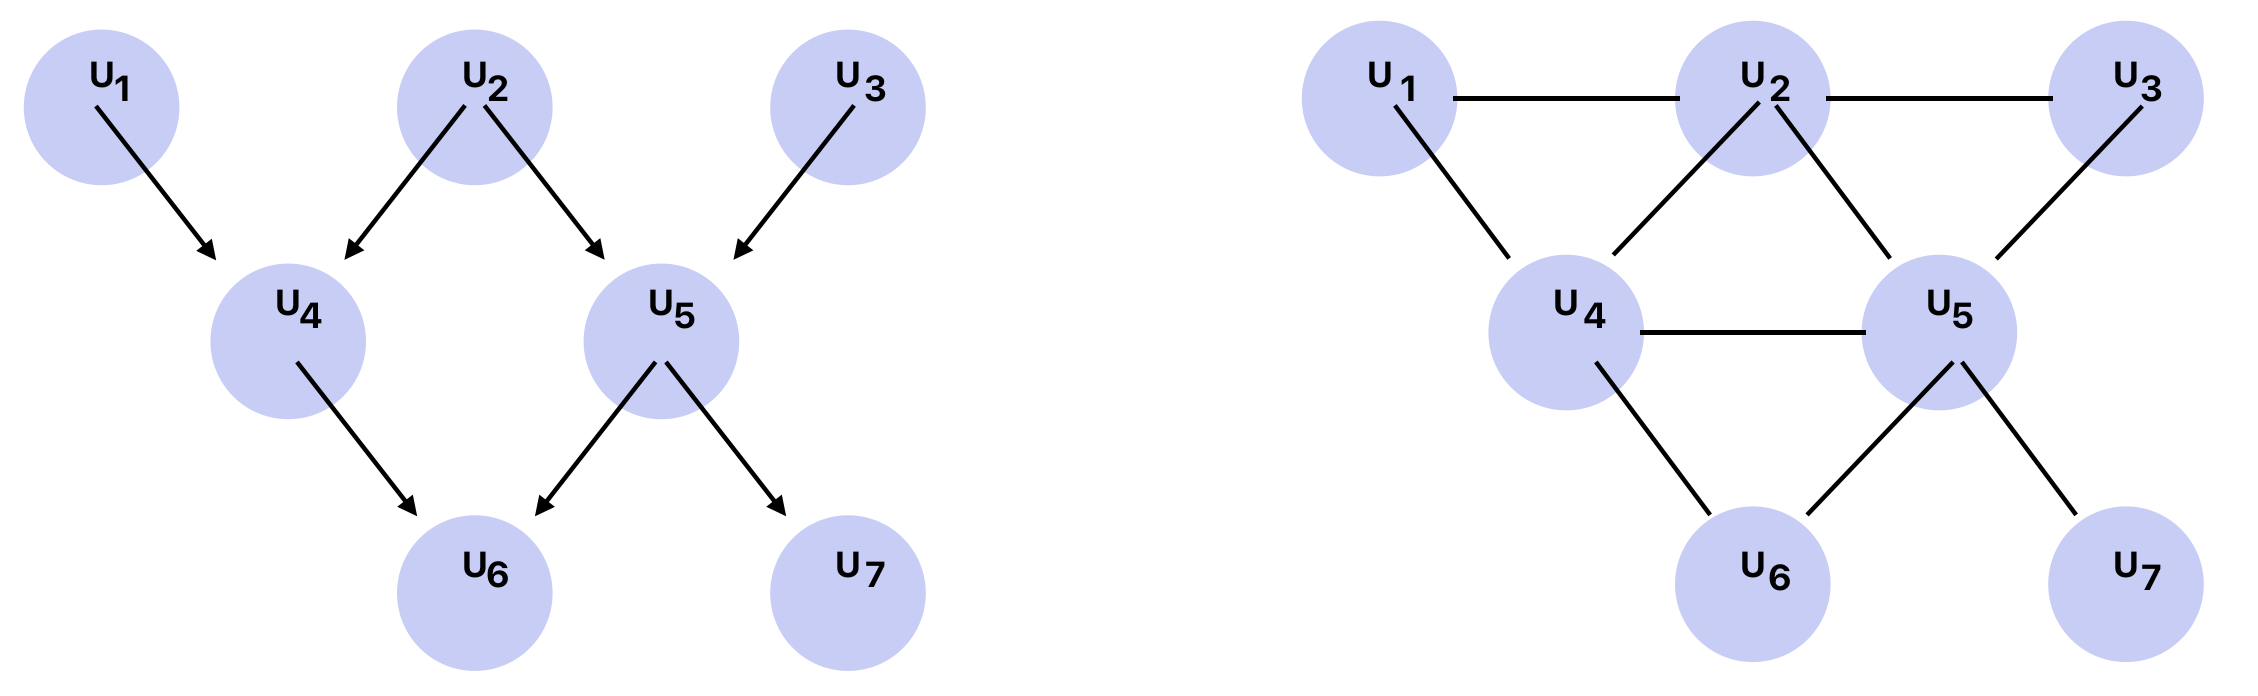
\includegraphics[width=1\linewidth]{Figures/GMRF Sparrows.png}
    \caption[Illustration of a pedigree as a GMRF]{Illustration of a pedigree as a GMRF, figure and figure text inspired by Figure 1 in \citet{Stensland_GMRF_bayes_animal_model}. On the left, a pedigree structure is depicted as a directed acyclic graph (DAG), where birds $U_1$ and $U_2$ are the parents of bird $U_4$, birds $U_2$ and $U_3$ the parents of bird $U_5$, and birds $U_4$ and $U_5$ the parents of bird $U_6$. Bird $U_7$ has one known parent in $U_5$, and one unknown. On the right, the conditional independence graph of the pedigree structure is given, where the parents sharing offspring is assigned an edge and the direction is removed.}
    \label{fig:GMRF_animal_model}
\end{figure}

% \subsection{Single and Multitrait Animal Model}
% When modelling the observed phenotypic trait values of individuals in a population, caution must be made when modelling the genetic component of the trait using INLA.
% If only one trait is considered, 
% The breeding values $\boldsymbol{\alpha}$ of an individual represents the genetic component of an observed phenotypic trait. 
% FINSIH THIS PART



% Would it be correct to interpret this as meaning that all the covariance is explained by relatedness, and that the additive variance is a scalar? Or is there a more complex covariance structure that might be present?

\cleardoublepage

%Regarding theory chapter:
%Need to decide if we back transform via lambda or not
%Need some feedback on the theory to make everything correct. 
%More specifically chapters 2.1, 2.5 and 3.1

\chapter{Methods}
\label{ch:method}
Based on the presented background theory, we now present our novel method for combining this into a relative variable importance tool for Bayesian GLMMs called Bayesian Variable importance (BVI). The proposed method is an extension of the method presented in \citet{Arnstad:Relative_variable_importance_in_Bayesian_linear_mixed_models:2024} so that it now applies to GLMMs modelled with binomial, Poisson in addition to Gaussian responses. The BVI method assumes the distinct random effects to be independent and does not include variable importance for random slopes.
\newline
\newline
For the complete model formulation of all methods used in this thesis, all files are uploaded to GitHub, with a link in \Cref{ap:github-repository}. 
% \subsection{Generalizing the relative weights method to GLMMs} 
% The presented theory on relative variable importance has mostly been developed for linear regression models. However, given the assumption of independence between fixed effects and random effects, we see no reason why the theory cannot be extended further. In \citet{matre}, the relative weights method was extended for the single random intercept model and showed promising results. Further, as long as the different random effects are independent, we argue that the variance estimates, when scaled by the response variance, directly correspond to their variance contribution. Utilizing the relative weights method for the fixed effects in a random intercept model using INLA was done in \citet{Arnstad:Relative_variable_importance_in_Bayesian_linear_mixed_models:2024} and a simulation study indicated that this method provides a proper decomposition of the $R^2$.
% DO I NEED TO BACK THIS LAST STATEMENT UP? IT IS BASICALLY "MY OPINION".
If categorical covariates with more than two levels are contained in the fixed effects, they should be encoded using distinct names in order to make sure the method can handle them correctly.
\section{Variable importance in the Bayesian framework}
There are a few considerations necessary in order to calculate variable importance on GLMMs in a Bayesian framework. Firstly, the characteristics of the Bayesian framework must be considered. When fitting a GLMM in the frequentist framework, point estimates of the fixed regression coefficients as well as point estimates of the variance of the random effects are obtained. These estimates are then used to calculate relative variable importance measures. In contrast, a Bayesian GLMM tries to estimate the joint posterior distribution of parameters. From the posterior distribution, one can obtain samples of all parameters, that can be used to approximate a posterior distribution for each parameter. It is these samples that we will use for further calculations.
% \\
% \\
% Further, the presented theory on relative variable importance has been developed for linear regression models. 
% However, given the assumption of independence between fixed effects and random effects, we see no reason why the theory cannot be extended further. In \citet{matre}, the relative weights method was extended for the random intercept model and showed promising results. The Bayesian analogue in \citet{Arnstad:Relative_variable_importance_in_Bayesian_linear_mixed_models:2024} utilized the relative weights method for the fixed effects in a random intercept model and a simulation study indicated that this method provides a proper decomposition of the $R^2$. 
% Moreover, as long as the distinct random effects are independent, we argue that the variance estimates, when scaled by the response variance, directly correspond to their proportion of explained variance. From this, we believe that the relative weights method can be applied to the fixed effects also in a GLMM.
\\
\\
Secondly, we argue that the most intuitive way to calculate variable importance is on the link (or latent) scale. The reasoning behind this is the definition of residual variance for models with additive overdispersion in \citet{nakagawa2013general}. This definition makes variable importance calculations on GLMMs analogous to that of LMMs, thus supporting a unified approach to both types of models. Therefore, we consider only GLMMs modeled with additive overdispersion, although we believe the method could be extended to handle multiplicative overdispersion as well.
These considerations are the basis of our proposed method for calculating relative variable importance in Bayesian GLMMs.
The presented method can handle categorical variables with more than two categories as long as they are dummy encoded. Random slopes are excluded from our method due to the added computational complexity and the debatable improvement of GLMMs and $R^2$ values with random slopes as mentioned in \citet{Johnson2014}.
We now go in to detail on how the different components of the GLMM model are handled in our method, to finally develop a relative importance measure for GLMMs.

% \subsection{Generalizing the relative weights method to } 
% Utilizing the relative weights method for the fixed effects in a random intercept model using INLA was done in \citet{Arnstad:Relative_variable_importance_in_Bayesian_linear_mixed_models:2024} and a simulation study indicated that this method provides a proper decomposition of the $R^2$.
% Given the assumption of independence between fixed effects and random effects, this method can be extended to any regression model, assuming appropriate considerations for a link function and random effects are addressed.
% DO I NEED TO BACK THIS LAST STATEMENT UP? IT IS BASICALLY "MY OPINION".

\section{Extending the \texorpdfstring{$R^2$}{Lg} to Bayesian GLMMs}
\label{sec:R2_Bayes_GLMM}
The core of our Bayesian variable importance measures is a decomposition of the $R^2$ value so that each covariate is assigned a share of relative variable importance. We now combine the definition of the $R^2$ for GLMMs presented \Cref{sec:R2_GLMM} and the $R^2$ for the Bayesian linear regression from \Cref{sec:bayes_R2} to yield our proposed distribution of the $R^2$ for Bayesian GLMMs. Consider the linear predictor 
\begin{equation}
    \label{eq:linear_predictor}
    g(\mathbb{E}[\mathbf{y}]) = g(\boldsymbol{\mu}) = \boldsymbol{\eta} = \mathbf{X}\boldsymbol{\beta} + \mathbf{U}\boldsymbol{\alpha} \ ,
\end{equation} 
for some response $\mathbf{y}$ and monotonic and differentiable link function $g(\cdot)$. 
The variance components of the linear predictor can be decomposed into variance from the fixed effects and the random effects. Define the variance of the fixed effects as 
\begin{equation}
    \sigma_{f}^2 = \text{Var}(\mathbf{X}\boldsymbol{\beta}) \ ,
\end{equation}
and let $\sigma^2_{\alpha_i}$ denote the variance of the $i$-th random effect, with random effects assumed independent. For Gaussian responses corresponding to an LMM, the residual variance $\sigma^2_{\varepsilon}$ is explicitly modelled as a parameter. The residual variance coincides with the overdispersion in the model, and the distributional variance with the identity link is zero \citep{nakagawa2013general}. However, for non-Gaussian responses, the residual variance of the model when considering additive overdispersion is defined as
\begin{equation}
    \sigma_{\varepsilon}^2 = \sigma^2_e + \sigma^2_d \ ,
\end{equation}
where $\sigma^2_e$ is the additive dispersion and $\sigma^2_d$ is the distributional variance \citep{nakagawa2013general}. A table containing the distributional variances for the link functions used in this thesis can be found in \Cref{table:1}. Given that we can obtain samples for the variance components, we define for a sample $s$ the marginal and conditional $R^2$ for the Bayesian GLMM as
\begin{equation}
    \label{eq:R2_Bayes_GLMM}
    R^2_{s, m} = \frac{\sigma_{f, s}^2}{\sigma_{f, s}^2 + \sum_{i=1}^q \sigma_{\alpha_i, s}^2 + \sigma_{\varepsilon, s}^2} \quad \text{and} \quad R^2_{s, c} = \frac{\sigma_{f, s}^2 + \sum_{i=1}^q \sigma_{\alpha_i, s}^2}{\sigma_{f, s}^2 + \sum_{i=1}^q \sigma_{\alpha_i, s}^2 + \sigma_{\varepsilon, s}^2} \ ,
\end{equation}
respectively, where $\sigma_{\varepsilon, s}^2 = \sigma^2_{e, s} + \sigma^2_{d, s}$ is the sampled residual variance. The posterior distribution of the marginal and conditional $R^2$ will then be approximated by the distribution of the samples of $R^2_{s, m}$ and $R^2_{s, c}$ for $s=1, ..., S$ respectively.

\begin{table}[ht]
    \centering
    \begin{tabular}{|c|c|c|c|}
    \hline
    \textbf{Distribution} &  \textbf{Link Function} & \textbf{Parameter} & \(\sigma^2_d\) \\
    \hline
    Gaussian & Identity & $\mu, \sigma^2 > 0$ & $0$ \\
    \hline
    Binomial & Logit & $0<p<1$ & \(\pi^2/3\) \\
    \hline
    %binomial & Probit &  1 \\
    %\hline
    Poisson & Log & $\lambda>0$ & $\ln(1 + 1/\mathbb{E}[\lambda])$ \\%\(\ln\left(1 + 1/\exp\left(\beta_0 + 0.5 (\sum_{k=1}^q \sigma_{\alpha_k}^2 + \sigma^2_e)\right) \right) \) \\
    % \hline
    % Poisson & Square Root & $\lambda>0$ & 0.25 \\
    \hline
    \end{tabular}
    \caption[Distribution-specific variance \(\sigma^2_d\) for the Gaussian, binomial and Poisson distributions]{Distribution-specific variance \(\sigma^2_d\) for the Gaussian, binomial and Poisson distributions with link functions. The full expression $\mathbb{E}[\lambda]$ is given in \eqref{eq:lambda}. Distributional variances correspond to the variances in \citet{nakagawa2013general} and the calculation for the log-link Poisson follow the recommendations of \citet{nakagawa2017}.}
    \label{table:1}
\end{table}


    
    


\section{Decomposing the \texorpdfstring{$R^2$}{Lg} value}
\label{sec:decomp_R2}
We now seek to decompose the proposed $R^2$ value and assign each covariate with a proportion of the variance explained, \textit{i.e.} assign each covariate with a \textit{relative variable importance}. Recall that the fixed and random effects are assumed to be independent, so that one can consider the variances of the fixed and random effects separately. Further, the residual variance, if present, is also considered as independent of both fixed and random effects. 
\subsection{Applying the relative weights method in the Bayesian framework}
To remedy the problems of calculating importance of correlated covariates, we will apply the relative weights method to the fixed effects before fitting the model. Following \Cref{sec:relativeweights}, we project the design matrix $\mathbf{X}$ of the fixed effects to obtain the matrix $\mathbf{Z}$. The model is fit using $\mathbf{Z}$ as an approximated design matrix of fixed effects, and from the joint posterior distribution samples of the coefficients $\boldsymbol{\beta}_{\mathbf{Z}}$ can be drawn. Each sample $\boldsymbol{\beta}_{\mathbf{Z}, s}, s=1, ..., S$ and the matrix $\mathbf{\Lambda}$ can be used to approximate a sample of the importance of the columns $\mathbf{X}$, with the squared entries of $\mathbf{\Lambda}$ acting as weights from the projected space to the original covariate space. Using equations \eqref{eq:lambda_rw} and \eqref{eq:RI_lambda}, we calculate this sample as
\begin{equation}
    \text{IMP}(\mathbf{X})_s = \boldsymbol{\Lambda}^{[2]} \boldsymbol{\beta}_{\mathbf{Z}, s}^{[2]} \ ,
\end{equation}
where $\text{IMP}(\mathbf{X})_s$ is a column vector containing the approximated importance of column $k$ of $\mathbf{X}$ on the $k$-th entry for $k=1, ..., p$ and $\boldsymbol{\xi}^{[2]}$ again denotes the Schur product of $\boldsymbol{\xi}$ with itself. To calculate the relative variable importance, note that we estimate $\sigma^2_{f, s}$ in \eqref{eq:R2_Bayes_GLMM} by
\begin{equation}
    \sigma^2_{f, s} \simeq \sum_{k=1}^{p}\text{IMP}(\mathbf{X})_{s, k}  \ . 
\end{equation}
Therefore, we define the relative importance of column $k$ of $\mathbf{X}$ in our method as
\begin{equation}
    \label{eq:RI_X}
    \text{RI}(\mathbf{X})_{s, k} = \frac{\text{IMP}(\mathbf{X})_{s, k}}{\sum_{j=1}^{p}\text{IMP}(\mathbf{X})_{s, j} + \sum_{i=1}^q \sigma_{\alpha_i, s}^2 + \sigma_{\varepsilon, s}^2} \ ,
\end{equation}
where $\sigma_{\alpha_i, s}^2$ and  $\sigma_{\varepsilon, s}^2$ are defined as in \Cref{sec:R2_Bayes_GLMM}.
For sufficiently large $S$, we believe these samples can be used to construct an approximation of the posterior distribution of the relative importance for each fixed effect. 

\subsection{Random effects}
The presented background theory on relative variable importance has mostly been developed for linear regression models. As long as the random effects are assumed not to be correlated, introducing random effects does not change the general idea. For each random effect, an approximation of the posterior distribution is constructed from the samples of the joint posterior distribution. Then, the proportion of variance explained by random effect $i$ for sample $s$ is calculated as 
\begin{equation}
    \label{eq:RI_alpha}
    \text{RI}(\alpha_i)_{s} = \frac{\sigma_{\alpha_i, s}^2}{\sum_{k=1}^{p}\text{IMP}(\mathbf{X})_{s, k} + \sum_{k=1}^q \sigma_{\alpha_k, s}^2 + \sigma_{\varepsilon, s}^2} \ .
\end{equation}
By sampling the relative importance for the random effects, we construct the approximated posterior distributions of relative importance.
In addition to the relative importance of the random effects, a quantity of interest is the intraclass correlation, often also called the within cluster correlation or repeatability \citep{GLMM_book}. The ICC represents the correlation between observations within the same cluster, and is defined for a random effect $\boldsymbol{\alpha}_i$ in \citep{nakagawa2017} as
\begin{equation}
    ICC = \frac{\sigma_{\alpha_i}^2}{\sum_{k=1}^{q}\sigma_{\alpha_k}^2 + \sigma_{\varepsilon}^2} \ .
\end{equation}
Thus, following the same logic as before we can sample the ICC as 
\begin{equation}
    \text{ICC}_s = \frac{\sigma_{\alpha_i, s}^2}{\sum_{k=1}^{q}\sigma_{\alpha_k, s}^2 + \sigma_{\varepsilon, s}^2} \ ,
\end{equation}
and obtain an approximate posterior distribution of the ICC. It is also worth noting that the distribution of relative importance of the distributional variance is calculated in the same manner. Although not a quantity of interest, it can give an indication of how influential the added variance from the specific distribution is with respect to the covariates.
\\
\\
As previously mentioned, it is common to report the precision of random effects rather than the variance. Since the random effects are assumed to be independent, one can invert the posterior mode of the precision distribution to obtain the variance. Another way of estimating the variance is to take the variance of the sampled values for the random vector $\boldsymbol{\alpha}$. Both methods seem to give very similar results as long as the sample size is large enough, and we therefore see both methods as fit for estimating the variance of random effects.
%In quantitative genetics, the ICC is of particular interest as it corresponds to the heritability of a trait.

\subsection{Drawing samples}
A critical part in performing the calculations required by the BVI method, is obtaining samples from the joint posterior distribution. To achieve this, we utilize the built-in function from the INLA framework called \texttt{inla.posterior.sample()}. This function uses the approximation of the posterior distribution fitted with INLA by numerical integration, and therefore, the accuracy of the samples depends on how well the numerical integration is carried out \citep{gomezrubio2020inla}. INLA provides several integration options, allowing one to choose the desired resolution at the cost of increased computational complexity. The BVI method is implemented using the default integration strategy in INLA, which is either the grid strategy for a hyperparameter vector of dimension less than or equal to two or the central composite design (CCD) for larger dimension hyperparameter vectors \citep{martino2019inla}. Further, if the model fit is poor or if the model is misspecified, the samples will also reflect these issues. Recall that INLA assumes a Gaussian latent layer, so this condition is crucial for obtaining a representative set of samples. We apply the simplified Laplace approximation when estimating the posterior marginals of the latent layer conditional on the hyperparameters, as is the default in INLA. However, one can choose among the three options provided in INLA, as described in \Cref{sec:INLA_marginals_approx} and \Cref{sec:INLA_parameter_estimation}. Lastly, note that INLA is a tool that is continuously in development, and therefore the method is subject to changes. For instance, the authors state that a skewness correction is in the works \citep{gomezrubio2020inla}, and more features are likely to be added in the future.

\section{Gaussian simulation study}
\label{sec:simulations}
To evaluate the performance of our proposed method a simulation study was conducted in \citet{Arnstad:Relative_variable_importance_in_Bayesian_linear_mixed_models:2024}, which we will reproduce here to provide a comprehensive overview. The study investigates how the BVI compares to the relative importance decomposition (\texttt{relaimpo}, see package description in \citet{groemping2023relaimpo}) as presented in \citet{gromping_relaimpo} and the two methods presented in \citet{matre}.
The Relaimpo method uses the LMG decomposition and considers only fixed effects and can therefore only be compared with the BVI in the fixed effects. The two methods in \citet{matre}, ELMG and the ERW, are extensions of the LMG and relative weights methods respectively, to include random intercepts.
These extensions allow us to compare the results for the random intercept model to our BVI method.
\newline
\newline
To simulate the data we consider the model as in \eqref{eq:linear_predictor}, with the link function $g(\cdot)$ being the identity function. We simulate $N=10^4$ responses, let $\boldsymbol{\alpha}=(\alpha_1, ..., \alpha_m)$ where $\alpha_j \stackrel{iid}{\sim} \mathcal{N}(0, \sigma^2_{\alpha})$ and $\sigma^2_{\alpha}=1$ as a single random intercept for $m=200$ clusters of $n_j=50$ observations each, $\mathbf{X} \sim \mathcal{N}(\boldsymbol{\mu},\Sigma) \in \mathbb{R}^{n \times p}$, where $\boldsymbol{\mu}=(1, 2, 3)$, $\Sigma_{ii} = 1, \Sigma_{i, k}=\rho_{i, k}, k\neq i$ and $p=3$ consisting of three fixed effects, $\mathbf{U}$ as a design matrix of appropriate dimension and a random error $\varepsilon_i \stackrel{iid}{\sim} \mathcal{N}(0, \sigma^2)$ with $\sigma^2=1$. 
Further, the true vector of regression coefficients is set to be set to be $\boldsymbol{\beta}=(1, \sqrt{2}, \sqrt{3})^T$ so the total model, including an intercept column of ones, can be written as
\begin{equation}
    \label{eq:simulation_model}
    \mathbf{y} = \mathbf{1} + \mathbf{X}\boldsymbol{\beta} + \mathbf{U}\boldsymbol{\alpha} + \boldsymbol{\varepsilon} \ .
\end{equation}
To investigate how different correlations between the fixed effects are handled by the method, we consider four different correlation levels between the fixed covariates in our data. That is achieved by letting $\rho_{1, 2} = \rho_{1, 3} = \rho_{2, 3}=\rho$ take on the values $\rho \in\{0, 0.1, 0.5, 0.9$\}.
For each correlation level, we simulate $N_{\text{sim}}=1000$ datasets and fit each of the four methods BVI, Relaimpo, ELMG and ERW.
To get a comparable measure from the Bayesian framework to the frequentist framework, we use the posterior means of the sampled posterior distribution of $\text{RI}(\mathbf{X})$ by the BVI method when estimating the quantities in  \eqref{eq:RI_X} and \eqref{eq:RI_alpha}.
\newline
\newline
From this setup, the total variance of the response is
\begin{equation}
    \label{eq:variance_theoretical_simulation}
    \text{Var}(\mathbf{y}) = \beta_{1}^2 + \beta_{2}^2 + \beta_{3}^2 + 2\sum_{i=1}^{3}\sum_{k=i+1}^{3} \beta_{i}\beta_{k}\rho_{ik} + \sigma_{\alpha}^2 + \sigma^2_{\varepsilon} \ , 
\end{equation}
and the theoretically expected relative importances for the case $\rho=0$ are
\begin{equation}
    \label{eq:RI_theoretical_simulation}
    \begin{aligned}
        \text{RI}(\mathbf{X}_1) = \text{RI}(\alpha) = \beta_{1}^2&  = \sigma^2_{\alpha} = \frac{1}{8} \hspace{1mm}, \hspace{1mm} \text{RI}(\mathbf{X}_2) = \beta_{2}^2 = \frac{2}{8} \hspace{1mm}, \hspace{1mm} \text{RI}(\mathbf{X}_3) = \beta_{3}^2 = \frac{3}{8} \ , 
    \end{aligned}
\end{equation}
by following the logic of \citet{gromping_relaimpo} and \citet{matre}. For correlated covariates however, the lack of consensus on an analytically sound decomposition of the $R^2$ value means we do not have theoretical values to compare with.
\\
\\
Further, the theoretically expected marginal $R^2$ values can be calculated as the variance of the fixed effects divided by the total variance given in \ref{eq:variance_theoretical_simulation}. Similarly, the expected conditional $R^2$ are given by the sum of variance of the fixed effects and random intercepts divided by the total variance. 
The expected $R^2$ values are listed in \Cref{table:2}.
\begin{table}[H]
    \centering
    \begin{tabular}{lrr}
    \hline
    $\rho$ & $\mathbb{E}[R^2_{\text{marg}}]$ & $\mathbb{E}[R^2_{\text{cond}}]$\\ 
    \hline
    $0$ & $0.750$ &  $0.875$ \\ 
    $0.1$ & $0.781$ & $0.890$ \\ 
    $0.5$ & $0.852$ & $0.926$\\ 
    $0.9$ & $0.889$ & $0.945$\\ 
    \hline
    \end{tabular}
    \caption[Expected $R^2$ for Gaussian LMM]{The theoretically expected marginal variance explained (left column) and conditional variance explained (right column) for different correlation levels between the fixed effects.}
    \label{table:2}
\end{table}
\noindent These values provide an empiric way of checking if our method fulfills the proper decomposition criteria listed in \Cref{sec:rel_imp}, by seeing if the relative importances for each effect sum to the model $R^2$.
% \newline
% It can here be noted that in the BVI method the approximated posterior marginals for each predictor, as well as the sampled posterior distribution of $\boldsymbol{\beta}_{\mathbf{Z}}$ and $\text{RI}(\mathbf{X})$, are available for each dataset. 


\section{Modelling phenotypic traits}
\label{sec:heritability_method}
% A particularly interesting application of variable importance, and an area of much active research, is estimating the heritability of phenotypic traits. As mentioned in \Cref{sec:animalmodel}, heritability is defined as the ratio of additive genetic variance to total phenotypic variance \citep{Wilson_heritability}. When modeling a phenotypic trait as the response, the variable importance of the random effect accounting for additive genetic variance can be interpreted as the heritability of the phenotypic trait. Therefore, this is a useful application of our variable importance method, and has been a key motivation for the development of the BVI method.
As we have seen in \Cref{sec:animalmodel}, the concept of variance decomposition in GLMMs is not new and has been used in quantitative genetics with the animal model for many years (\textit{e.g.} \citet{Kruuk2004}). The main quantity of interest in such studies is often the heritability of phenotypic traits, which is defined as the ratio of additive genetic variance to total phenotypic variance \citep{Wilson_heritability}. We now aim to illustrate how the heritability of phenotypic traits becomes readily accessible using the BVI method, and hence illustrating why heritability is a special case of variable importance. This also involves modelling a pedigree covariance structure in random effects, which is a pivotal feature of the BVI method.
% \\
% \\
% To demonstrate the broader and more extensive inference possible with the BVI method, we present the estimated posterior distributions of relative importance for all covariates here. For more detailed plots of the estimated posterior heritability distributions, see \Cref{ap:supplementary}.
% To demonstrate the broader inference possible with the BVI method, we have added the estimated posterior distributions of relative importance for all covariates in the supplementary material \Cref{ap:supplementary}. As heritability is a well-known quantity in quantitative genetics, there exists many other studies to compare our results with. Therefore, we investigate only the heritability estimates, but also want to emphasize that the BVI method is capable of providing more extensive inference on all covariates. 
\subsection{Heritability as relative variable importance}
By comparing \eqref{eq:h2} with \eqref{eq:RI_alpha}, it is clear that the way we have defined relative variable importance of a random effect coincides with the definition of heritability, if the random effect is the additive genetic effect and one assumes the total phenotypic variance $\sigma^2_P$ to be captured by the other fixed and random effects present. Therefore, when applying the BVI method to model a phenotypic trait, the relative variable importance of the random effect accounting for additive genetic variance can be interpreted as the heritability of the phenotypic trait. This is a highly relevant and useful application of our method and has been a major motivation for the development of the BVI method. It should be mentioned here that in the frequentist framework, fixed effects are assumed to not have an associated variance. Therefore, fixed effects are commonly not featured in formulae for the variance decomposition when estimating heritability (see \citet{Kruuk2004} and \citet{Wilson_guide_animal_model}). Further, the discrimination between fixed and random effects are not always clear in biology. Often, no variance component of fixed effects is calculated. This means that they do not go into the calculation of the total phenotypic variance. However, there may be effects that are modelled as fixed, but still contribute to the phenotypic variance. To avoid confusion on this topic, we have implemented our method such that any covariate that contributes with variance in the model, is included in the calculation of total phenotypic variance. We see this to be the most clear and general way to handle the problem.
% The parameters of interest are now the additive genetic variance $\sigma^2_A$ and the \textbf{heritability}, defined as the proportion of the total phenotypic variance that is present due to the additive genetic variance, $\sigma^2_A/\sigma^2_P$ \citep{Wilson2008}.
% \section{Case studies}
% To illustrate and evaluate our proposed method, we perform several case studies. The first case study investigates how the method performs on real data from a study on house sparrows (\textit{Passer domesticus}) and compares to the study in \citet{Stensland_GMRF_bayes_animal_model}. The second case study applies the method to a Gaussian, a Poisson and a binomial GLMM, and compares the results to the vignette of the \texttt{rptR} package found at \url{https://cran.r-project.org/web/packages/rptR/vignettes/rptR.html} and described in \citet{Stoffel2017rptR}. The two aforementioned case studies investigate the heritability of traits and repeatability of clusters respectively. 
% \\
% \\
% Either:
% \\
% \\
% Therefore, we perform a third case study on a simulated dataset, in which we know the true values and can therefore evaluate the variable importance for all parameters. In this study, we model the Poisson and binomial GLMMs, and refer to \citet{Arnstad:Relative_variable_importance_in_Bayesian_linear_mixed_models:2024} for a simulation study on Gaussian LMMs using the same methodology.
% \\
% \\
% Or:
% \\
% \\
% For calculations of the importance on other covariates, we refer to the simulation study in \citet{Arnstad:Relative_variable_importance_in_Bayesian_linear_mixed_models:2024}. This study covers the method for the LMMs and has shown promising results of a proper decomposition of the $R^2$ value.
\subsection{House sparrow study}
We now apply the BVI method to a dataset gathered on house sparrows (\textit{Passer domesticus}) from a study on the coast of Helgeland, Norway \citep{Stensland_GMRF_bayes_animal_model}. The entire bird population on five islands have been surveyed since 1993 and several morphological traits have been measured. Blood samples were drawn to determine the relatedness between birds, and we therefore have a pedigree structure for the birds \citep[citing Jensen et al., 2003, 2004, 2008]{Stensland_GMRF_bayes_animal_model}. In the dataset we use we have $N=3116$ birds with one or more observations on the traits and covariates. For a more thorough description of the house sparrow study, see \citet[and references therein]{Stensland_GMRF_bayes_animal_model}. We model three phenotypic traits using a Gaussian LMM, namely the body mass, wing length and tarsus length. The fixed effects in the model consist of observations of \textit{sex}, a standardized inbreeding coefficient denoted \textit{FGRM}, the standardized \textit{month} of the year (measurements were made during May-August), the \textit{age} of each bird, and dummy variables encoding the location of the \textit{native island} group of the bird (three levels, inner islands, outer islands or other islands). In addition, we model the \textit{hatchyear}  as an independent and identically distributed (i.i.d.) random intercept. To account for the correlation between relatives, we include a random effect for the additive genetic variance called \textit{IDC2}. It is the sampled variances of the additive genetic random effect that will determine the heritability of each trait. We derive the relatedness matrix of the birds from our pedigree, and specify the inverse as the precision matrix for the additive genetic variance term. Lastly, to account for individual differences we add an i.i.d. random intercept, denoted by \textit{IDC}, for the individual bird. We prefer to use the INLA framework, described in \Cref{sec:INLA_framework}, to fit our LMM as it is computationally efficient and easy to use. Each prior is internally parametrized in INLA by $\theta=\ln(\tau)$ with $\tau$ being the precision of the prior. This means when placing priors, they are always placed on the scale of the internal parameter $\theta$, and if we want to place a prior on the external scale we must take this into account. For the fixed effects, we place penalising complexity (PC) priors with parameters $U=\sqrt{2}$ and $a=0.05$ as the input parameters discussed in section \Cref{seq:PC_prior}. Similarly, we place PC priors on each random effect, with the effects \textit{hatchyear} and \textit{IDC} having $U=1$ and $a=0.05$.  The additive genetic effect, \textit{IDC2}, is assigned $U=\sqrt{2}$ and $a=0.05$. These priors have been chosen through discussion with the supervisor of the thesis and researchers with domain knowledge in biology. We draw $N_{\text{samp}}=10^4$ samples from the posterior distribution of the Bayesian GLMM fitted with the BVI method to estimate the posterior relative importances of the covariates.

\section{Non-Gaussian studies}
In this section, we present the methodology used to apply the Bayesian Variable Importance method to non-Gaussian GLMMs. This is a key extension of the method, as it allows the method to handle a wider range of models. We will analyse the binomial and Poisson GLMMs, both via a simulation study and a case study.
\\
\\
To evaluate the performance of the BVI method, we will use analytic results when possible, \textit{i.e.} for uncorrelated covariates and $R^2$ estimates. For correlated covariates, there is no consensus on an analytically correct method to allocate the shared variance among correlated fixed effects \citep{gromping_relaimpo}. Further, we also compare the results with the \texttt{rptR} package \citep{Stoffel2017rptR}, implemented in the frequentist framework. This package was originally designed to calculate the repeatability of phenotypic traits, which is closely related to relative variable importance. The main difference in capabilities between the BVI method and that of the \texttt{rptR} package, is that the BVI method estimates the relative importance distribution of each fixed effect, whereas the \texttt{rptR} package estimates only the sum of fixed effects importances. Due to this difference, our comparisons involve the estimates of relative importance for the random effects. We also compare the marginal $R^2$ and conditional $R^2$ with \texttt{rptR}, as these measures correspond to the sum of fixed effects importances and the aggregated importances of fixed and random effects, respectively.
\subsection{Binomial and Poisson simulation studies}
\label{sec:simulation_study}
There are three primary reasons why we wish to conduct a simulation study with our method. The first being the ability to evaluate how well our method assigns relative variable importance to all covariates in the model. The real life case studies available mostly have the heritability, or some other function of the additive genetic variance, as the objective of analysis \citep{Stensland_GMRF_bayes_animal_model}. We aim to provide the heritability, but at the same time provide information on the relative variable importance of all covariates present in the model. The second motivation is that the Bayesian framework is stochastic, and so is our method. We wish to assess the variability of this stochasticity by simulating different datasets with the same underlying structure, and evaluate the spread of the estimates from the BVI method. We hope that this can provide signs that any fitted model can be seen as a random sample of a distribution centered around the true value. Lastly, the fundamental challenge that variable importance measures face, is the task of allocating the part of the variance explained due to correlation between covariates. Therefore, we wish to evaluate how our model performs for different correlation levels. This will give insight into how robust it is, and if the method handles correlated covariates in a sensible manner.
\\
\\
%and a binomial distribution with a probit link.
We simulate $N=10^4$ responses from a binomial distribution with a logit-link and from a Poisson distribution with log-link. The linear predictor contains three fixed effects and one random intercept. The fixed effects are, for simplicity but without loss of generalization, $\mathbf{X} \sim \mathcal{N}(\boldsymbol{\mu}, \Sigma)$ with $\boldsymbol{\mu} = (0, 0, 0)^T$, $\Sigma_{i, i} = 1$ and $\Sigma_{i, k} = \rho, k \neq i$. The true regression coefficient for the binomial model are set to be $\boldsymbol{\beta}=(1, \sqrt{2}, \sqrt{3})^T$. In the binomial model, the random effect $\boldsymbol{\alpha}=(\alpha_1, ..., \alpha_m)$ comes from $m=100$ clusters, each with $n_j=100$ observations for $j=1, ..., m$. Further, we draw the random effect from a normal distribution such that $\alpha_j \stackrel{iid}{\sim} \mathcal{N}(0, \sigma^2_{\alpha})$, with $\sigma^2_{\alpha}=1$. This means that the total variance of the linear predictor $\boldsymbol{\eta}$ is $\sigma_{\eta}^2=7$. For the Poisson model, to avoid numerical instabilities, it was necessary to standardize the linear predictor used in the simulation study. Thus, the true regression coefficients were set to be $\boldsymbol{\beta}=\frac{1}{\sqrt{7}}(1, \sqrt{2}, \sqrt{3})^T$ and the random effect $\alpha_j \stackrel{iid}{\sim} \mathcal{N}(0, \sigma^2_{\alpha})$ now with $\sigma^2_{\alpha}=1/7$. To investigate the impact of correlated fixed effects, we fit five different models letting $\rho$ vary for each model by taking on the values $\rho \in \{-0.4, -0.1, 0, 0.1, 0.4\}$. The INLA framework is used to fit the GLMMs and the methodology described used to calculate the relative importance. All fixed and random effects receive the same PC prior with parameters $U=1$ and $a=0.01$. We fit $N_{\text{sim}}=500$ binomial and Poisson models with different datasets for each correlation level. For each fitted model, the posterior modes of the quantities of interest are used to estimate the relative importance of the covariates, as well as marginal and conditional $R^2$.
\\
\\
%For the binomial simulation with distributional variance $\sigma^2_d$ independent of the fitted model
In the simulation study, when parameters are simulated so that we know their true value, we can analytically calculate the relative importance of the parameters when they are not correlated. When uncorrelated, the proportion of variance explained by each fixed effect in the linear predictor is equal to the square of the true coefficient divided by the total model variance on latent scale. The proportion of variance explained by the random effect is simply its variance divided by the total model variance on latent scale. By defining $\sigma_{x_k}^2$ as the variance contribution to the linear predictor for fixed effect $k$ and $\sigma^2_{\alpha}$ as the variance contribution of the random effect, we then have for the binomial model with logit-link
\begin{equation}
    \sigma_{x_1}^2 = \sigma_{\alpha}^2  = 1 \quad \text{and} \quad \sigma_{x_2}^2 = 2 \quad \text{and} \quad \sigma_{x_3}^2 = 3 \ ,
\end{equation}
and for the Poisson model with log-link
\begin{equation}
    \sigma_{x_1}^2 = \sigma_{\alpha}^2  = 1/7 \quad \text{and} \quad \sigma_{x_2}^2 = 2/7 \quad \text{and} \quad \sigma_{x_3}^2 = 3/7 \ .
\end{equation}
Then, the relative importance of the covariates can be calculated by following \Cref{sec:decomp_R2} as
\begin{equation}
    \begin{aligned}
        \text{RI}(\mathbf{X}_{1})  = \text{RI}(\alpha_1)  &= \frac{\sigma_{x_1}^2}{\sum_{i=1}^{3}\sigma_{x_i}^2 +\sigma_{\alpha_1}^2  + \sigma_d^2}, \\
        \text{RI}(\mathbf{X}_2) &= \frac{\sigma_{x_3}^2}{\sum_{i=1}^{3}\sigma_{x_i}^2 +\sigma_{\alpha_1}^2 +  \sigma_d^2}, \\
        \text{RI}(\mathbf{X}_3) &= \frac{\sigma_{x_3}^2}{\sum_{i=1}^{3}\sigma_{x_i}^2 +\sigma_{\alpha_1}^2 +  \sigma_d^2} \ .
    \end{aligned}
\end{equation}
In our simulation study, the binomial model with logit-link is assigned $\sigma^2_d=\pi^2/3$ as in \Cref{table:1}. The distributional variance of the Poisson model with log-link is given by 
\begin{equation}
    \sigma_d^2 = \ln (1 + 1/\mathbb{E}[\mathbf{y}]) = \ln (1 + 1/\mathbb{E}[\lambda]) \ ,
\end{equation}
with
\begin{equation}
    \label{eq:lambda}
    \mathbb{E}[\lambda]=\exp\left(\beta_0 + 0.5 \sigma^2_{\tau}\right) \ ,
\end{equation}
being the quantity used in \Cref{table:1} and where $\sigma^2_{\tau}$ denotes the total model variance on the latent scale \citep{nakagawa2017}. So we obtain, using a single random intercept, $\sigma_{d}^2=0.4741$ with $\beta_0=0$, $\sigma^2_{\tau}=1$. Therefore, we can summarize the expected relative importance of our three models as in \Cref{table:3}. Recall that for correlated covariates, no consensus exists, and we therefore have no analytical results to compare with.
\begin{table}[H]
    \centering
    \begin{tabular}{lrrrr}
    \hline
    \textbf{Model} & $\mathbb{E}[\text{RI}(\boldsymbol{\alpha})]$ & $\mathbb{E}[\text{RI}(\mathbf{X}_{1})]$ & $\mathbb{E}[\text{RI}(\mathbf{X}_{2})]$ & $\mathbb{E}[\text{RI}(\mathbf{X}_{3})]$\\ 
    \hline
    Binomial Logit & 0.0972 & 0.0972 & 0.1944 & 0.2915 \\ 
    %binomial, probit & 0.1250 & 0.1250 & 0.2500 & 0.3750 \\ 
    Poisson Log & 0.0969 & 0.0969 & 0.1938 & 0.2907 \\ 
    \hline
    \end{tabular}
    \caption[Expected relative importance of independent covariates for non-Gaussian GLMMs]{The theoretically expected relative importance of the covariates on the latent scale in the different models when they are uncorrelated.}
    \label{table:3}
\end{table}
\noindent In practice, the distributional variance of the Poisson model should be calculated using the estimated values, and the distributional variance will therefore be dependent on the fitted model \citep{nakagawa2017}.
\\
\\
In addition to the expected importance of covariates in the uncorrelated case, we can calculate the expected marginal and conditional $R^2$ values for all correlation levels on the latent scale. Recalling that each of the $p=3$ columns of $\mathbf{X}$ is initialized to have variance equal to $1$, the expected marginal $R^2$ can be calculated as
\begin{equation}
    \mathbb{E}[R^2_{\text{marg}}] = \frac{\sum_{i=1}^{3} \beta_i^2 + 2 \sum_{i=1}^{2}\sum_{k=i+1}^{3}\beta_i\beta_k \rho}{\sum_{i=1}^{3} \beta_i^2 + 2 \sum_{i=1}^{2}\sum_{k=i+1}^{3}\beta_i\beta_k \rho + \sigma^2_{\alpha} + \sigma_d^2} \ ,
\end{equation}
and similarly for the expected conditional $R^2$ as
\begin{equation}
    \mathbb{E}[R^2_{\text{cond}}] = \frac{\sum_{i=1}^{3} \beta_i^2 + 2 \sum_{i=1}^{2}\sum_{k=i+1}^{3}\beta_i\beta_k \rho + \sigma^2_{\alpha}}{\sum_{i=1}^{3} \beta_i^2 + 2 \sum_{i=1}^{2}\sum_{k=i+1}^{3}\beta_i\beta_k \rho + \sigma^2_{\alpha} + \sigma_d^2} \ .
\end{equation}
\begin{table}[H]
    \centering
    \begin{tabular}{lcccccc}
    \toprule
    \textbf{Model Type} & \textbf{Correlation (\(\rho\))} & $\mathbb{E}[R^2_{\text{marg}}]$ &  $\mathbb{E}[R^2_{\text{cond}}]$ \\
    \midrule
    Binomial Logit & -0.4 & 0.262 & 0.434 \\
    Binomial Logit & -0.1 & 0.532 & 0.641 \\
    Binomial Logit & 0    & 0.583 & 0.680 \\
    Binomial Logit & 0.1  & 0.624 & 0.712 \\
    Binomial Logit & 0.4  & 0.709 & 0.777 \\
    \midrule
    Poisson Log  & -0.4 & 0.225 & 0.373 \\
    Poisson Log  & -0.1 & 0.518 & 0.625 \\
    Poisson Log  & 0    & 0.581 & 0.678 \\
    Poisson Log  & 0.1  & 0.634 & 0.723 \\
    Poisson Log  & 0.4  & 0.747 & 0.820 \\
    \bottomrule
    \end{tabular}
    \caption[Expected $R^2$ for non-Gaussian GLMMs]{Theoretically expected marginal and conditional $R^2$ values on the latent scale for the binomial regression with logit-link (top) and Poisson regression with log-link (bottom) for different correlation levels $\rho$.}
    \label{table:r2values}
\end{table}

\subsection{Binomial and Poisson case studies}
To further investigate how well the BVI method generalizes to non-Gaussian responses, we perform a case study using the setup described in the vignette of the R-package \texttt{rptR}, found at \url{https://cran.r-project.org/web/packages/rptR/vignettes/rptR.html} \citep{Stoffel2017rptR}. 
%This package estimates the repeatability of phenotypic traits, which is closely related to heritability. 
As mentioned, this package was developed, in the frequentist framework, to estimate the repeatability of phenotypic traits.
An important clarification for this case study, is that there are multiple formulations of repeatability. Two of the most common ways of looking at repeatability are
\begin{equation}
    \begin{aligned}
        \text{R}_1 &= \frac{\text{Additive genetic variance}}{\text{Total variance of covariates}} \\
        \text{R}_2 &= \frac{\text{Additive genetic variance}}{\text{Total variance of random covariates}} \ ,
    \end{aligned}
\end{equation}
where the former corresponds to our notion of heritability \citep{Stoffel2017rptR} and the latter to the ICC \citep{GLMM_book}. We choose to look at the notion corresponding to heritability, and to obtain the result from \texttt{rptR} so that they match this, each model must be fit with the argument \texttt{adjusted=FALSE} \citep{Stoffel2017rptR}. The dataset used in the \texttt{rptR} package vignette, introduced for a different purpose, is simulated to replicate a study on twelve different beetle larvae populations \citep{Stoffel2017rptR}. It contains $N=960$ observations of the covariates \textit{population}, the discrete \textit{habitat} of the larvae, the dietary \textit{treatment} of the larvae, the \textit{sex} and \textit{container} of which the larvae were contained in. The phenotypes to be modeled by the binomial and Poisson distributions are the two distinct male color morphs and the number of eggs laid by female larvae respectively. Both models use \textit{treatment} as the only fixed effect and place i.i.d. random intercepts on the \textit{population} and \textit{container} covariates. Note that a more complex covariance structure could be modelled by the BVI method, but the \texttt{rptR} package does not allow for this, so for comparing the methods we see it as suitable with i.i.d. random intercepts. As before, our modelling is carried out using INLA, whereas the models in the vignette are calculated from functions in the \texttt{rptR} package. The priors placed by the BVI method on the fixed effect \textit{treatment} and random effects \textit{population} and \textit{container} are PC priors with parameters $U=1$ and $a=0.01$. Furthermore, we also here draw $N_{\text{samp}}=10^4$ samples from the posterior distribution of the Bayesian GLMM fitted with the BVI method to estimate the posterior distributions of the repeatability. 
% \section{Simulation study with \texorpdfstring{$R^2$}{Lg}-induced Dirichlet decomposition priors and Generalized Decomposition Priors on \texorpdfstring{$R^2$}{Lg}}
\section{Simulation Study with Dirichlet and Generalized Decomposition Priors on \texorpdfstring{$R^2$}{Lg}}
\label{sec:r2d2method}
As mentioned, the literature on Bayesian variable importance is not very comprehensive. However, as discussed in \Cref{sec:R2D2}, the R2D2 and GDR2 priors decompose the $R^2$ value and can therefore be interpreted as a variable importance measure. We find it sensible to try and compare the resulting variable importance distributions, even though the R2D2 and GDR2 priors have not been developed for this goal specifically. To be able to evaluate the two measures, we simulate a linear regression model with $p=3$ covariates and $N=1000$ observations. The covariates are for simplicity simulated as $\mathbf{X} \sim \mathcal{N}(\boldsymbol{\mu}, \boldsymbol{\Sigma})$ with $\boldsymbol{\mu} = (0, 0, 0)^T$, $\boldsymbol{\Sigma}_{i, i} = 1$ and $\boldsymbol{\Sigma}_{i, j} = \rho$ for $i \neq j$. As before, we vary the correlation by letting $\rho \in \{-0.4, -0.1, 0, 0.1, 0.4\}$. The true regression coefficients are initialized as $\boldsymbol{\beta} = (1, \sqrt{2}, \sqrt{3})$, and we simulate a random error by $\varepsilon \sim \mathcal{N}(0, \sigma^2)$ with $\sigma^2=1$. By noting that $\text{Var}(\mathbf{y}) = 7$ in the uncorrelated case, it is clear that the expected relative importance of the independent covariates can be calculated as
\begin{equation}
    \label{eq:RI_R2D2}
    \text{RI}(\mathbf{X})_{1} =  \frac{1}{7} \quad \text{RI}(\mathbf{X})_{2} =  \frac{2}{7} \quad  \text{RI}(\mathbf{X})_{3} =  \frac{3}{7} \ .
\end{equation}
Further, the $R^2$ for this model is by the definition in \eqref{eq:R2}
\begin{equation}
    R^2 = \frac{\text{Var}(\mathbf{y}) - \sigma^2}{\text{Var}(\mathbf{y})} \ ,
\end{equation}
which gives expected values that are summarized in \Cref{table:r2values_r2d2}.
\begin{table}[H]
    \centering
    \begin{tabular}{lcc}
    \toprule
    \textbf{\(\rho\)} & $R^2$  \\
    \midrule
    -0.4 & 0.604 \\
    -0.1 & 0.830 \\
    0    & 0.857 \\
    0.1  & 0.877 \\
    0.4  & 0.913 \\
    \bottomrule
    \end{tabular}
    \caption[Expected $R^2$ for comparison of BVI and shrinkage prior methods]{Theoretically expected $R^2$ values for the correlation levels $\rho$ used in the linear regression for analyzing the BVI method in comparison to the R2D2 priors.}
    \label{table:r2values_r2d2}
\end{table}
\noindent To fit the linear regression using R2D2 priors for the marginal $R^2$ we use functions from the GitHub repository \citet{zhang2024r2d2_git} by the author of \citet{zhang2020bayesian}. For the GDR2 priors, we utilize the Stan code available on \citet{aguilar2024GDR_code} by the authors of \citet{aguilar2024generalized}. The hyperparameters for the marginal $R^2 \sim \text{Beta}(a, b)$ are set so that $\mathbb{E}[R^2] \simeq 0.857$ which is approximately the theoretical $R^2$ of uncorrelated covariates. This is done for the R2D2 priors by using the default value $b=0.5$ from \citet{zhang2024r2d2_git} and noting that the expected value of the $\text{Beta}(a, b)$ distribution is $a/(a+b)$ \citep{stats_book}. We employ the Gibbs sampler for the marginal R2D2 prior as described in \citep[section 5.3]{zhang2020bayesian} and run the MCMC iteration $N_{\text{samp}}=10^4$ times, with a burn in of $9000$ samples which are discarded. This gives $1000$ samples from the posterior distribution of the marginal $R^2$ as well as $1000$ samples of each $\phi_j$ for $j=1, 2, 3$. The BVI method draws the same number of samples for the covariates from the posterior distribution of the fitted Bayesian GLMM, using PC priors with $U=1$ and $a=0.01$ for all covariates.
For the GDR2 priors, the implementation requires a prior on the expected value and the precision of the $R^2$ value directly. These are calculated by letting $a_{\pi}=0.7$, the reference unit $\alpha_K$ be zero, the expected $R^2$ equal $6/7$ and then solving for the precision $\tau$ according to the properties of the Beta distribution given in \citet{aguilar2024generalized}. The choice of $a_{\pi}$ corresponds to a scenario in which one assumes the covariates to be approximately equally important and the difference between the GDR2 prior and R2D2 prior is substantial \citep{aguilar2024generalized}. Similarly, as for the R2D2 case, we run the MCMC iteration $N_{\text{samp}}=10^4$ times, with a burn in of $9000$ samples, but we also fit four Markov chains this time to ensure proper mixing. This means we obtain $4000$ samples for the GDR2 priors. The samples of $\phi_j$ from the linear regression using R2D2 and GDR2 priors are then seen as the posterior distribution of relative variable importance of $\mathbf{x}_j$, and compared to the corresponding distributions estimated from the BVI method. We will refer to the results by using R2D2 and GDR2 priors as the R2D2 method and the GDR2 method respectively. To evaluate all methods, we fit a frequentist linear regression model and evaluate the importance metrics according to the LMG method by using the package \texttt{relaimpo} \citep{groemping2023relaimpo} in R as described in \citet{gromping_relaimpo}. As the LMG is feasible in this context, it poses perhaps the most robust and reliable benchmark available. We draw $1000$ bootstrap samples of the LMG metrics and use this to create confidence intervals for the importance estimates. 



% This means that the expected relative importance in the binomial model with probit link of $X_1$ and $\alpha_1$ is $1/8$ and the expected relative importance of $X_2$ and $X_3$ is $2/8$ and $3/8$ respectively. For the logit link we have an expected relative importance of $0.0972$ for $X_1$ and $\alpha_1$, $0.194$ for $X_2$ and $0.292$ for $X_3$.
% For the Poisson simulation however, the distributional variance is approximated by $\sigma_d^2 = \ln (1 + 1/\mathbb{E}[\lambda])$ with $\mathbb{E}[\lambda]=\exp\left(\beta_0 + 0.5 (\sum_{k=1}^q \sigma_{\alpha_k}^2 + \sigma^2_e)\right)$, and is therefore dependent on the fitted model \citep{nakagawa2017}. 

% All data is standardized before fitting the models, so that 
% \begin{equation}
%     \sigma_{x_1}^2 = \sigma_{\alpha_1}^2 = \sigma_{\alpha_2}^2 = \frac{1}{9}
% \end{equation}

% The total variance of $\boldsymbol{\eta}$ from this setup can be found as 
% \begin{equation}
%     \text{Var}(\boldsymbol{\eta}) = \beta_{1, \mathbf{X}}^2 + \beta_{2, \mathbf{X}}^2 + \beta_{3, \mathbf{X}}^2 + 2\sum_{j=1}^{3}\sum_{k=j+1}^{3} \beta_{j, \mathbf{X}}\beta_{k, \mathbf{X}}\rho_{jk} + \sigma_{\alpha_1}^2 + \sigma_{\alpha_2}^2 + \sigma^2_{\varepsilon} \ .
% \end{equation}
% For the uncorrelated case ($\rho=0$) we can find that this equals 
% \begin{equation}
%     \text{Var}(\boldsymbol{\eta}) = 1 + 2 + 3 + 1 + 1 + 1 =  9 \ ,
% \end{equation}
% meaning that in the linear predictor we have 
% \begin{equation}
%     \text{RI}(\mathbf{x}_1) = \text{RI}(\alpha_1) = \text{RI}(\alpha_2) = \frac{1}{9}, \quad \text{RI}(\mathbf{x}_2) = \frac{2}{9}, \quad \text{RI}(\mathbf{x}_3) = \frac{3}{9} \ .
% \end{equation}
% We must now account for the distributional variance, which is independent of the relative contributions. 

% and we must now define the distribution specific variance. For the Poisson distribution with log-link, we approximate the distribution specific variance as in \Cref{table:1} with values obtained from the fitted model. The binomial distribution with probit link is assigned a distributional variance of $1$.
% \begin{equation}
%     \sigma^2_d = 
%     \begin{cases} 
%         \ln\left(1 + \frac{1}{\exp(2)}\right) = 0.127 & \text{for the log-link}, \\
%         1 & \text{for the probit link}.
%     \end{cases}
% \end{equation}
% and therefore we can calculate the relative variance contribution on latent scale, i.e. how we calculate relative variable importance, for each covariate as 
% \begin{equation}
%     \text{RI}(\mathbf{x}_1) = \text{RI}(\alpha_1) = \text{RI}(\alpha_2) = \frac{1}{\text{Var}(\boldsymbol{\eta})}, \quad \text{RI}(\mathbf{x}_2) = \frac{2}{\text{Var}(\boldsymbol{\eta})}, \quad \text{RI}(\mathbf{x}_3) = \frac{3}{\text{Var}(\boldsymbol{\eta})} \ .
% \end{equation}
% \\
% \\
% We fit four different models, letting $\rho$ vary for each model by taking on the values $0, 0.1, 0.5$ and $0.9$. The INLA framework is used to fit the GLMMs and the methodology described used to calculate the relative importance.

% \begin{table}[ht]
%     \centering
%     \begin{tabular}{lrr}
%     \hline
%     $\rho$ & $R^2_{\text{marg}}$ & $R^2_{\text{cond}}$\\ 
%     \hline
%     $0$ & $0.750$ &  $0.875$ \\ 
%     $0.1$ & $0.781$ & $0.890$ \\ 
%     $0.5$ & $0.852$ & $0.926$\\ 
%     $0.9$ & $0.889$ & $0.945$\\ 
%     \hline
%     \end{tabular}
%     \caption{The theoretically correct marginal variance explained (left column) and conditional variance explained (right column) for different correlation levels between the fixed effects.}
%     \label{table:2}
% \end{table}


\cleardoublepage

% \chapter{Methods}
% \label{ch:method}
% Based on the presented background theory, we now present our novel method for combining this into a relative variable importance tool for Bayesian GLMMs called Bayesian Variable importance (BVI). The proposed method is an extension of the method presented in \citet{Arnstad:Relative_variable_importance_in_Bayesian_linear_mixed_models:2024} so that it now applies to GLMMs modelled with binomial, Poisson in addition to Gaussian responses. The BVI method assumes the distinct random effects to be independent and does not include variable importance for random slopes.
\newline
\newline
For the complete model formulation of all methods used in this thesis, all files are uploaded to GitHub, with a link in \Cref{ap:github-repository}. 
% \subsection{Generalizing the relative weights method to GLMMs} 
% The presented theory on relative variable importance has mostly been developed for linear regression models. However, given the assumption of independence between fixed effects and random effects, we see no reason why the theory cannot be extended further. In \citet{matre}, the relative weights method was extended for the single random intercept model and showed promising results. Further, as long as the different random effects are independent, we argue that the variance estimates, when scaled by the response variance, directly correspond to their variance contribution. Utilizing the relative weights method for the fixed effects in a random intercept model using INLA was done in \citet{Arnstad:Relative_variable_importance_in_Bayesian_linear_mixed_models:2024} and a simulation study indicated that this method provides a proper decomposition of the $R^2$.
% DO I NEED TO BACK THIS LAST STATEMENT UP? IT IS BASICALLY "MY OPINION".
If categorical covariates with more than two levels are contained in the fixed effects, they should be encoded using distinct names in order to make sure the method can handle them correctly.
\section{Variable importance in the Bayesian framework}
There are a few considerations necessary in order to calculate variable importance on GLMMs in a Bayesian framework. Firstly, the characteristics of the Bayesian framework must be considered. When fitting a GLMM in the frequentist framework, point estimates of the fixed regression coefficients as well as point estimates of the variance of the random effects are obtained. These estimates are then used to calculate relative variable importance measures. In contrast, a Bayesian GLMM tries to estimate the joint posterior distribution of parameters. From the posterior distribution, one can obtain samples of all parameters, that can be used to approximate a posterior distribution for each parameter. It is these samples that we will use for further calculations.
% \\
% \\
% Further, the presented theory on relative variable importance has been developed for linear regression models. 
% However, given the assumption of independence between fixed effects and random effects, we see no reason why the theory cannot be extended further. In \citet{matre}, the relative weights method was extended for the random intercept model and showed promising results. The Bayesian analogue in \citet{Arnstad:Relative_variable_importance_in_Bayesian_linear_mixed_models:2024} utilized the relative weights method for the fixed effects in a random intercept model and a simulation study indicated that this method provides a proper decomposition of the $R^2$. 
% Moreover, as long as the distinct random effects are independent, we argue that the variance estimates, when scaled by the response variance, directly correspond to their proportion of explained variance. From this, we believe that the relative weights method can be applied to the fixed effects also in a GLMM.
\\
\\
Secondly, we argue that the most intuitive way to calculate variable importance is on the link (or latent) scale. The reasoning behind this is the definition of residual variance for models with additive overdispersion in \citet{nakagawa2013general}. This definition makes variable importance calculations on GLMMs analogous to that of LMMs, thus supporting a unified approach to both types of models. Therefore, we consider only GLMMs modeled with additive overdispersion, although we believe the method could be extended to handle multiplicative overdispersion as well.
These considerations are the basis of our proposed method for calculating relative variable importance in Bayesian GLMMs.
The presented method can handle categorical variables with more than two categories as long as they are dummy encoded. Random slopes are excluded from our method due to the added computational complexity and the debatable improvement of GLMMs and $R^2$ values with random slopes as mentioned in \citet{Johnson2014}.
We now go in to detail on how the different components of the GLMM model are handled in our method, to finally develop a relative importance measure for GLMMs.

% \subsection{Generalizing the relative weights method to } 
% Utilizing the relative weights method for the fixed effects in a random intercept model using INLA was done in \citet{Arnstad:Relative_variable_importance_in_Bayesian_linear_mixed_models:2024} and a simulation study indicated that this method provides a proper decomposition of the $R^2$.
% Given the assumption of independence between fixed effects and random effects, this method can be extended to any regression model, assuming appropriate considerations for a link function and random effects are addressed.
% DO I NEED TO BACK THIS LAST STATEMENT UP? IT IS BASICALLY "MY OPINION".

\section{Extending the \texorpdfstring{$R^2$}{Lg} to Bayesian GLMMs}
\label{sec:R2_Bayes_GLMM}
The core of our Bayesian variable importance measures is a decomposition of the $R^2$ value so that each covariate is assigned a share of relative variable importance. We now combine the definition of the $R^2$ for GLMMs presented \Cref{sec:R2_GLMM} and the $R^2$ for the Bayesian linear regression from \Cref{sec:bayes_R2} to yield our proposed distribution of the $R^2$ for Bayesian GLMMs. Consider the linear predictor 
\begin{equation}
    \label{eq:linear_predictor}
    g(\mathbb{E}[\mathbf{y}]) = g(\boldsymbol{\mu}) = \boldsymbol{\eta} = \mathbf{X}\boldsymbol{\beta} + \mathbf{U}\boldsymbol{\alpha} \ ,
\end{equation} 
for some response $\mathbf{y}$ and monotonic and differentiable link function $g(\cdot)$. 
The variance components of the linear predictor can be decomposed into variance from the fixed effects and the random effects. Define the variance of the fixed effects as 
\begin{equation}
    \sigma_{f}^2 = \text{Var}(\mathbf{X}\boldsymbol{\beta}) \ ,
\end{equation}
and let $\sigma^2_{\alpha_i}$ denote the variance of the $i$-th random effect, with random effects assumed independent. For Gaussian responses corresponding to an LMM, the residual variance $\sigma^2_{\varepsilon}$ is explicitly modelled as a parameter. The residual variance coincides with the overdispersion in the model, and the distributional variance with the identity link is zero \citep{nakagawa2013general}. However, for non-Gaussian responses, the residual variance of the model when considering additive overdispersion is defined as
\begin{equation}
    \sigma_{\varepsilon}^2 = \sigma^2_e + \sigma^2_d \ ,
\end{equation}
where $\sigma^2_e$ is the additive dispersion and $\sigma^2_d$ is the distributional variance \citep{nakagawa2013general}. A table containing the distributional variances for the link functions used in this thesis can be found in \Cref{table:1}. Given that we can obtain samples for the variance components, we define for a sample $s$ the marginal and conditional $R^2$ for the Bayesian GLMM as
\begin{equation}
    \label{eq:R2_Bayes_GLMM}
    R^2_{s, m} = \frac{\sigma_{f, s}^2}{\sigma_{f, s}^2 + \sum_{i=1}^q \sigma_{\alpha_i, s}^2 + \sigma_{\varepsilon, s}^2} \quad \text{and} \quad R^2_{s, c} = \frac{\sigma_{f, s}^2 + \sum_{i=1}^q \sigma_{\alpha_i, s}^2}{\sigma_{f, s}^2 + \sum_{i=1}^q \sigma_{\alpha_i, s}^2 + \sigma_{\varepsilon, s}^2} \ ,
\end{equation}
respectively, where $\sigma_{\varepsilon, s}^2 = \sigma^2_{e, s} + \sigma^2_{d, s}$ is the sampled residual variance. The posterior distribution of the marginal and conditional $R^2$ will then be approximated by the distribution of the samples of $R^2_{s, m}$ and $R^2_{s, c}$ for $s=1, ..., S$ respectively.

\begin{table}[ht]
    \centering
    \begin{tabular}{|c|c|c|c|}
    \hline
    \textbf{Distribution} &  \textbf{Link Function} & \textbf{Parameter} & \(\sigma^2_d\) \\
    \hline
    Gaussian & Identity & $\mu, \sigma^2 > 0$ & $0$ \\
    \hline
    Binomial & Logit & $0<p<1$ & \(\pi^2/3\) \\
    \hline
    %binomial & Probit &  1 \\
    %\hline
    Poisson & Log & $\lambda>0$ & $\ln(1 + 1/\mathbb{E}[\lambda])$ \\%\(\ln\left(1 + 1/\exp\left(\beta_0 + 0.5 (\sum_{k=1}^q \sigma_{\alpha_k}^2 + \sigma^2_e)\right) \right) \) \\
    % \hline
    % Poisson & Square Root & $\lambda>0$ & 0.25 \\
    \hline
    \end{tabular}
    \caption[Distribution-specific variance \(\sigma^2_d\) for the Gaussian, binomial and Poisson distributions]{Distribution-specific variance \(\sigma^2_d\) for the Gaussian, binomial and Poisson distributions with link functions. The full expression $\mathbb{E}[\lambda]$ is given in \eqref{eq:lambda}. Distributional variances correspond to the variances in \citet{nakagawa2013general} and the calculation for the log-link Poisson follow the recommendations of \citet{nakagawa2017}.}
    \label{table:1}
\end{table}


    
    


\section{Decomposing the \texorpdfstring{$R^2$}{Lg} value}
\label{sec:decomp_R2}
We now seek to decompose the proposed $R^2$ value and assign each covariate with a proportion of the variance explained, \textit{i.e.} assign each covariate with a \textit{relative variable importance}. Recall that the fixed and random effects are assumed to be independent, so that one can consider the variances of the fixed and random effects separately. Further, the residual variance, if present, is also considered as independent of both fixed and random effects. 
\subsection{Applying the relative weights method in the Bayesian framework}
To remedy the problems of calculating importance of correlated covariates, we will apply the relative weights method to the fixed effects before fitting the model. Following \Cref{sec:relativeweights}, we project the design matrix $\mathbf{X}$ of the fixed effects to obtain the matrix $\mathbf{Z}$. The model is fit using $\mathbf{Z}$ as an approximated design matrix of fixed effects, and from the joint posterior distribution samples of the coefficients $\boldsymbol{\beta}_{\mathbf{Z}}$ can be drawn. Each sample $\boldsymbol{\beta}_{\mathbf{Z}, s}, s=1, ..., S$ and the matrix $\mathbf{\Lambda}$ can be used to approximate a sample of the importance of the columns $\mathbf{X}$, with the squared entries of $\mathbf{\Lambda}$ acting as weights from the projected space to the original covariate space. Using equations \eqref{eq:lambda_rw} and \eqref{eq:RI_lambda}, we calculate this sample as
\begin{equation}
    \text{IMP}(\mathbf{X})_s = \boldsymbol{\Lambda}^{[2]} \boldsymbol{\beta}_{\mathbf{Z}, s}^{[2]} \ ,
\end{equation}
where $\text{IMP}(\mathbf{X})_s$ is a column vector containing the approximated importance of column $k$ of $\mathbf{X}$ on the $k$-th entry for $k=1, ..., p$ and $\boldsymbol{\xi}^{[2]}$ again denotes the Schur product of $\boldsymbol{\xi}$ with itself. To calculate the relative variable importance, note that we estimate $\sigma^2_{f, s}$ in \eqref{eq:R2_Bayes_GLMM} by
\begin{equation}
    \sigma^2_{f, s} \simeq \sum_{k=1}^{p}\text{IMP}(\mathbf{X})_{s, k}  \ . 
\end{equation}
Therefore, we define the relative importance of column $k$ of $\mathbf{X}$ in our method as
\begin{equation}
    \label{eq:RI_X}
    \text{RI}(\mathbf{X})_{s, k} = \frac{\text{IMP}(\mathbf{X})_{s, k}}{\sum_{j=1}^{p}\text{IMP}(\mathbf{X})_{s, j} + \sum_{i=1}^q \sigma_{\alpha_i, s}^2 + \sigma_{\varepsilon, s}^2} \ ,
\end{equation}
where $\sigma_{\alpha_i, s}^2$ and  $\sigma_{\varepsilon, s}^2$ are defined as in \Cref{sec:R2_Bayes_GLMM}.
For sufficiently large $S$, we believe these samples can be used to construct an approximation of the posterior distribution of the relative importance for each fixed effect. 

\subsection{Random effects}
The presented background theory on relative variable importance has mostly been developed for linear regression models. As long as the random effects are assumed not to be correlated, introducing random effects does not change the general idea. For each random effect, an approximation of the posterior distribution is constructed from the samples of the joint posterior distribution. Then, the proportion of variance explained by random effect $i$ for sample $s$ is calculated as 
\begin{equation}
    \label{eq:RI_alpha}
    \text{RI}(\alpha_i)_{s} = \frac{\sigma_{\alpha_i, s}^2}{\sum_{k=1}^{p}\text{IMP}(\mathbf{X})_{s, k} + \sum_{k=1}^q \sigma_{\alpha_k, s}^2 + \sigma_{\varepsilon, s}^2} \ .
\end{equation}
By sampling the relative importance for the random effects, we construct the approximated posterior distributions of relative importance.
In addition to the relative importance of the random effects, a quantity of interest is the intraclass correlation, often also called the within cluster correlation or repeatability \citep{GLMM_book}. The ICC represents the correlation between observations within the same cluster, and is defined for a random effect $\boldsymbol{\alpha}_i$ in \citep{nakagawa2017} as
\begin{equation}
    ICC = \frac{\sigma_{\alpha_i}^2}{\sum_{k=1}^{q}\sigma_{\alpha_k}^2 + \sigma_{\varepsilon}^2} \ .
\end{equation}
Thus, following the same logic as before we can sample the ICC as 
\begin{equation}
    \text{ICC}_s = \frac{\sigma_{\alpha_i, s}^2}{\sum_{k=1}^{q}\sigma_{\alpha_k, s}^2 + \sigma_{\varepsilon, s}^2} \ ,
\end{equation}
and obtain an approximate posterior distribution of the ICC. It is also worth noting that the distribution of relative importance of the distributional variance is calculated in the same manner. Although not a quantity of interest, it can give an indication of how influential the added variance from the specific distribution is with respect to the covariates.
\\
\\
As previously mentioned, it is common to report the precision of random effects rather than the variance. Since the random effects are assumed to be independent, one can invert the posterior mode of the precision distribution to obtain the variance. Another way of estimating the variance is to take the variance of the sampled values for the random vector $\boldsymbol{\alpha}$. Both methods seem to give very similar results as long as the sample size is large enough, and we therefore see both methods as fit for estimating the variance of random effects.
%In quantitative genetics, the ICC is of particular interest as it corresponds to the heritability of a trait.

\subsection{Drawing samples}
A critical part in performing the calculations required by the BVI method, is obtaining samples from the joint posterior distribution. To achieve this, we utilize the built-in function from the INLA framework called \texttt{inla.posterior.sample()}. This function uses the approximation of the posterior distribution fitted with INLA by numerical integration, and therefore, the accuracy of the samples depends on how well the numerical integration is carried out \citep{gomezrubio2020inla}. INLA provides several integration options, allowing one to choose the desired resolution at the cost of increased computational complexity. The BVI method is implemented using the default integration strategy in INLA, which is either the grid strategy for a hyperparameter vector of dimension less than or equal to two or the central composite design (CCD) for larger dimension hyperparameter vectors \citep{martino2019inla}. Further, if the model fit is poor or if the model is misspecified, the samples will also reflect these issues. Recall that INLA assumes a Gaussian latent layer, so this condition is crucial for obtaining a representative set of samples. We apply the simplified Laplace approximation when estimating the posterior marginals of the latent layer conditional on the hyperparameters, as is the default in INLA. However, one can choose among the three options provided in INLA, as described in \Cref{sec:INLA_marginals_approx} and \Cref{sec:INLA_parameter_estimation}. Lastly, note that INLA is a tool that is continuously in development, and therefore the method is subject to changes. For instance, the authors state that a skewness correction is in the works \citep{gomezrubio2020inla}, and more features are likely to be added in the future.

\section{Gaussian simulation study}
\label{sec:simulations}
To evaluate the performance of our proposed method a simulation study was conducted in \citet{Arnstad:Relative_variable_importance_in_Bayesian_linear_mixed_models:2024}, which we will reproduce here to provide a comprehensive overview. The study investigates how the BVI compares to the relative importance decomposition (\texttt{relaimpo}, see package description in \citet{groemping2023relaimpo}) as presented in \citet{gromping_relaimpo} and the two methods presented in \citet{matre}.
The Relaimpo method uses the LMG decomposition and considers only fixed effects and can therefore only be compared with the BVI in the fixed effects. The two methods in \citet{matre}, ELMG and the ERW, are extensions of the LMG and relative weights methods respectively, to include random intercepts.
These extensions allow us to compare the results for the random intercept model to our BVI method.
\newline
\newline
To simulate the data we consider the model as in \eqref{eq:linear_predictor}, with the link function $g(\cdot)$ being the identity function. We simulate $N=10^4$ responses, let $\boldsymbol{\alpha}=(\alpha_1, ..., \alpha_m)$ where $\alpha_j \stackrel{iid}{\sim} \mathcal{N}(0, \sigma^2_{\alpha})$ and $\sigma^2_{\alpha}=1$ as a single random intercept for $m=200$ clusters of $n_j=50$ observations each, $\mathbf{X} \sim \mathcal{N}(\boldsymbol{\mu},\Sigma) \in \mathbb{R}^{n \times p}$, where $\boldsymbol{\mu}=(1, 2, 3)$, $\Sigma_{ii} = 1, \Sigma_{i, k}=\rho_{i, k}, k\neq i$ and $p=3$ consisting of three fixed effects, $\mathbf{U}$ as a design matrix of appropriate dimension and a random error $\varepsilon_i \stackrel{iid}{\sim} \mathcal{N}(0, \sigma^2)$ with $\sigma^2=1$. 
Further, the true vector of regression coefficients is set to be set to be $\boldsymbol{\beta}=(1, \sqrt{2}, \sqrt{3})^T$ so the total model, including an intercept column of ones, can be written as
\begin{equation}
    \label{eq:simulation_model}
    \mathbf{y} = \mathbf{1} + \mathbf{X}\boldsymbol{\beta} + \mathbf{U}\boldsymbol{\alpha} + \boldsymbol{\varepsilon} \ .
\end{equation}
To investigate how different correlations between the fixed effects are handled by the method, we consider four different correlation levels between the fixed covariates in our data. That is achieved by letting $\rho_{1, 2} = \rho_{1, 3} = \rho_{2, 3}=\rho$ take on the values $\rho \in\{0, 0.1, 0.5, 0.9$\}.
For each correlation level, we simulate $N_{\text{sim}}=1000$ datasets and fit each of the four methods BVI, Relaimpo, ELMG and ERW.
To get a comparable measure from the Bayesian framework to the frequentist framework, we use the posterior means of the sampled posterior distribution of $\text{RI}(\mathbf{X})$ by the BVI method when estimating the quantities in  \eqref{eq:RI_X} and \eqref{eq:RI_alpha}.
\newline
\newline
From this setup, the total variance of the response is
\begin{equation}
    \label{eq:variance_theoretical_simulation}
    \text{Var}(\mathbf{y}) = \beta_{1}^2 + \beta_{2}^2 + \beta_{3}^2 + 2\sum_{i=1}^{3}\sum_{k=i+1}^{3} \beta_{i}\beta_{k}\rho_{ik} + \sigma_{\alpha}^2 + \sigma^2_{\varepsilon} \ , 
\end{equation}
and the theoretically expected relative importances for the case $\rho=0$ are
\begin{equation}
    \label{eq:RI_theoretical_simulation}
    \begin{aligned}
        \text{RI}(\mathbf{X}_1) = \text{RI}(\alpha) = \beta_{1}^2&  = \sigma^2_{\alpha} = \frac{1}{8} \hspace{1mm}, \hspace{1mm} \text{RI}(\mathbf{X}_2) = \beta_{2}^2 = \frac{2}{8} \hspace{1mm}, \hspace{1mm} \text{RI}(\mathbf{X}_3) = \beta_{3}^2 = \frac{3}{8} \ , 
    \end{aligned}
\end{equation}
by following the logic of \citet{gromping_relaimpo} and \citet{matre}. For correlated covariates however, the lack of consensus on an analytically sound decomposition of the $R^2$ value means we do not have theoretical values to compare with.
\\
\\
Further, the theoretically expected marginal $R^2$ values can be calculated as the variance of the fixed effects divided by the total variance given in \ref{eq:variance_theoretical_simulation}. Similarly, the expected conditional $R^2$ are given by the sum of variance of the fixed effects and random intercepts divided by the total variance. 
The expected $R^2$ values are listed in \Cref{table:2}.
\begin{table}[H]
    \centering
    \begin{tabular}{lrr}
    \hline
    $\rho$ & $\mathbb{E}[R^2_{\text{marg}}]$ & $\mathbb{E}[R^2_{\text{cond}}]$\\ 
    \hline
    $0$ & $0.750$ &  $0.875$ \\ 
    $0.1$ & $0.781$ & $0.890$ \\ 
    $0.5$ & $0.852$ & $0.926$\\ 
    $0.9$ & $0.889$ & $0.945$\\ 
    \hline
    \end{tabular}
    \caption[Expected $R^2$ for Gaussian LMM]{The theoretically expected marginal variance explained (left column) and conditional variance explained (right column) for different correlation levels between the fixed effects.}
    \label{table:2}
\end{table}
\noindent These values provide an empiric way of checking if our method fulfills the proper decomposition criteria listed in \Cref{sec:rel_imp}, by seeing if the relative importances for each effect sum to the model $R^2$.
% \newline
% It can here be noted that in the BVI method the approximated posterior marginals for each predictor, as well as the sampled posterior distribution of $\boldsymbol{\beta}_{\mathbf{Z}}$ and $\text{RI}(\mathbf{X})$, are available for each dataset. 


\section{Modelling phenotypic traits}
\label{sec:heritability_method}
% A particularly interesting application of variable importance, and an area of much active research, is estimating the heritability of phenotypic traits. As mentioned in \Cref{sec:animalmodel}, heritability is defined as the ratio of additive genetic variance to total phenotypic variance \citep{Wilson_heritability}. When modeling a phenotypic trait as the response, the variable importance of the random effect accounting for additive genetic variance can be interpreted as the heritability of the phenotypic trait. Therefore, this is a useful application of our variable importance method, and has been a key motivation for the development of the BVI method.
As we have seen in \Cref{sec:animalmodel}, the concept of variance decomposition in GLMMs is not new and has been used in quantitative genetics with the animal model for many years (\textit{e.g.} \citet{Kruuk2004}). The main quantity of interest in such studies is often the heritability of phenotypic traits, which is defined as the ratio of additive genetic variance to total phenotypic variance \citep{Wilson_heritability}. We now aim to illustrate how the heritability of phenotypic traits becomes readily accessible using the BVI method, and hence illustrating why heritability is a special case of variable importance. This also involves modelling a pedigree covariance structure in random effects, which is a pivotal feature of the BVI method.
% \\
% \\
% To demonstrate the broader and more extensive inference possible with the BVI method, we present the estimated posterior distributions of relative importance for all covariates here. For more detailed plots of the estimated posterior heritability distributions, see \Cref{ap:supplementary}.
% To demonstrate the broader inference possible with the BVI method, we have added the estimated posterior distributions of relative importance for all covariates in the supplementary material \Cref{ap:supplementary}. As heritability is a well-known quantity in quantitative genetics, there exists many other studies to compare our results with. Therefore, we investigate only the heritability estimates, but also want to emphasize that the BVI method is capable of providing more extensive inference on all covariates. 
\subsection{Heritability as relative variable importance}
By comparing \eqref{eq:h2} with \eqref{eq:RI_alpha}, it is clear that the way we have defined relative variable importance of a random effect coincides with the definition of heritability, if the random effect is the additive genetic effect and one assumes the total phenotypic variance $\sigma^2_P$ to be captured by the other fixed and random effects present. Therefore, when applying the BVI method to model a phenotypic trait, the relative variable importance of the random effect accounting for additive genetic variance can be interpreted as the heritability of the phenotypic trait. This is a highly relevant and useful application of our method and has been a major motivation for the development of the BVI method. It should be mentioned here that in the frequentist framework, fixed effects are assumed to not have an associated variance. Therefore, fixed effects are commonly not featured in formulae for the variance decomposition when estimating heritability (see \citet{Kruuk2004} and \citet{Wilson_guide_animal_model}). Further, the discrimination between fixed and random effects are not always clear in biology. Often, no variance component of fixed effects is calculated. This means that they do not go into the calculation of the total phenotypic variance. However, there may be effects that are modelled as fixed, but still contribute to the phenotypic variance. To avoid confusion on this topic, we have implemented our method such that any covariate that contributes with variance in the model, is included in the calculation of total phenotypic variance. We see this to be the most clear and general way to handle the problem.
% The parameters of interest are now the additive genetic variance $\sigma^2_A$ and the \textbf{heritability}, defined as the proportion of the total phenotypic variance that is present due to the additive genetic variance, $\sigma^2_A/\sigma^2_P$ \citep{Wilson2008}.
% \section{Case studies}
% To illustrate and evaluate our proposed method, we perform several case studies. The first case study investigates how the method performs on real data from a study on house sparrows (\textit{Passer domesticus}) and compares to the study in \citet{Stensland_GMRF_bayes_animal_model}. The second case study applies the method to a Gaussian, a Poisson and a binomial GLMM, and compares the results to the vignette of the \texttt{rptR} package found at \url{https://cran.r-project.org/web/packages/rptR/vignettes/rptR.html} and described in \citet{Stoffel2017rptR}. The two aforementioned case studies investigate the heritability of traits and repeatability of clusters respectively. 
% \\
% \\
% Either:
% \\
% \\
% Therefore, we perform a third case study on a simulated dataset, in which we know the true values and can therefore evaluate the variable importance for all parameters. In this study, we model the Poisson and binomial GLMMs, and refer to \citet{Arnstad:Relative_variable_importance_in_Bayesian_linear_mixed_models:2024} for a simulation study on Gaussian LMMs using the same methodology.
% \\
% \\
% Or:
% \\
% \\
% For calculations of the importance on other covariates, we refer to the simulation study in \citet{Arnstad:Relative_variable_importance_in_Bayesian_linear_mixed_models:2024}. This study covers the method for the LMMs and has shown promising results of a proper decomposition of the $R^2$ value.
\subsection{House sparrow study}
We now apply the BVI method to a dataset gathered on house sparrows (\textit{Passer domesticus}) from a study on the coast of Helgeland, Norway \citep{Stensland_GMRF_bayes_animal_model}. The entire bird population on five islands have been surveyed since 1993 and several morphological traits have been measured. Blood samples were drawn to determine the relatedness between birds, and we therefore have a pedigree structure for the birds \citep[citing Jensen et al., 2003, 2004, 2008]{Stensland_GMRF_bayes_animal_model}. In the dataset we use we have $N=3116$ birds with one or more observations on the traits and covariates. For a more thorough description of the house sparrow study, see \citet[and references therein]{Stensland_GMRF_bayes_animal_model}. We model three phenotypic traits using a Gaussian LMM, namely the body mass, wing length and tarsus length. The fixed effects in the model consist of observations of \textit{sex}, a standardized inbreeding coefficient denoted \textit{FGRM}, the standardized \textit{month} of the year (measurements were made during May-August), the \textit{age} of each bird, and dummy variables encoding the location of the \textit{native island} group of the bird (three levels, inner islands, outer islands or other islands). In addition, we model the \textit{hatchyear}  as an independent and identically distributed (i.i.d.) random intercept. To account for the correlation between relatives, we include a random effect for the additive genetic variance called \textit{IDC2}. It is the sampled variances of the additive genetic random effect that will determine the heritability of each trait. We derive the relatedness matrix of the birds from our pedigree, and specify the inverse as the precision matrix for the additive genetic variance term. Lastly, to account for individual differences we add an i.i.d. random intercept, denoted by \textit{IDC}, for the individual bird. We prefer to use the INLA framework, described in \Cref{sec:INLA_framework}, to fit our LMM as it is computationally efficient and easy to use. Each prior is internally parametrized in INLA by $\theta=\ln(\tau)$ with $\tau$ being the precision of the prior. This means when placing priors, they are always placed on the scale of the internal parameter $\theta$, and if we want to place a prior on the external scale we must take this into account. For the fixed effects, we place penalising complexity (PC) priors with parameters $U=\sqrt{2}$ and $a=0.05$ as the input parameters discussed in section \Cref{seq:PC_prior}. Similarly, we place PC priors on each random effect, with the effects \textit{hatchyear} and \textit{IDC} having $U=1$ and $a=0.05$.  The additive genetic effect, \textit{IDC2}, is assigned $U=\sqrt{2}$ and $a=0.05$. These priors have been chosen through discussion with the supervisor of the thesis and researchers with domain knowledge in biology. We draw $N_{\text{samp}}=10^4$ samples from the posterior distribution of the Bayesian GLMM fitted with the BVI method to estimate the posterior relative importances of the covariates.

\section{Non-Gaussian studies}
In this section, we present the methodology used to apply the Bayesian Variable Importance method to non-Gaussian GLMMs. This is a key extension of the method, as it allows the method to handle a wider range of models. We will analyse the binomial and Poisson GLMMs, both via a simulation study and a case study.
\\
\\
To evaluate the performance of the BVI method, we will use analytic results when possible, \textit{i.e.} for uncorrelated covariates and $R^2$ estimates. For correlated covariates, there is no consensus on an analytically correct method to allocate the shared variance among correlated fixed effects \citep{gromping_relaimpo}. Further, we also compare the results with the \texttt{rptR} package \citep{Stoffel2017rptR}, implemented in the frequentist framework. This package was originally designed to calculate the repeatability of phenotypic traits, which is closely related to relative variable importance. The main difference in capabilities between the BVI method and that of the \texttt{rptR} package, is that the BVI method estimates the relative importance distribution of each fixed effect, whereas the \texttt{rptR} package estimates only the sum of fixed effects importances. Due to this difference, our comparisons involve the estimates of relative importance for the random effects. We also compare the marginal $R^2$ and conditional $R^2$ with \texttt{rptR}, as these measures correspond to the sum of fixed effects importances and the aggregated importances of fixed and random effects, respectively.
\subsection{Binomial and Poisson simulation studies}
\label{sec:simulation_study}
There are three primary reasons why we wish to conduct a simulation study with our method. The first being the ability to evaluate how well our method assigns relative variable importance to all covariates in the model. The real life case studies available mostly have the heritability, or some other function of the additive genetic variance, as the objective of analysis \citep{Stensland_GMRF_bayes_animal_model}. We aim to provide the heritability, but at the same time provide information on the relative variable importance of all covariates present in the model. The second motivation is that the Bayesian framework is stochastic, and so is our method. We wish to assess the variability of this stochasticity by simulating different datasets with the same underlying structure, and evaluate the spread of the estimates from the BVI method. We hope that this can provide signs that any fitted model can be seen as a random sample of a distribution centered around the true value. Lastly, the fundamental challenge that variable importance measures face, is the task of allocating the part of the variance explained due to correlation between covariates. Therefore, we wish to evaluate how our model performs for different correlation levels. This will give insight into how robust it is, and if the method handles correlated covariates in a sensible manner.
\\
\\
%and a binomial distribution with a probit link.
We simulate $N=10^4$ responses from a binomial distribution with a logit-link and from a Poisson distribution with log-link. The linear predictor contains three fixed effects and one random intercept. The fixed effects are, for simplicity but without loss of generalization, $\mathbf{X} \sim \mathcal{N}(\boldsymbol{\mu}, \Sigma)$ with $\boldsymbol{\mu} = (0, 0, 0)^T$, $\Sigma_{i, i} = 1$ and $\Sigma_{i, k} = \rho, k \neq i$. The true regression coefficient for the binomial model are set to be $\boldsymbol{\beta}=(1, \sqrt{2}, \sqrt{3})^T$. In the binomial model, the random effect $\boldsymbol{\alpha}=(\alpha_1, ..., \alpha_m)$ comes from $m=100$ clusters, each with $n_j=100$ observations for $j=1, ..., m$. Further, we draw the random effect from a normal distribution such that $\alpha_j \stackrel{iid}{\sim} \mathcal{N}(0, \sigma^2_{\alpha})$, with $\sigma^2_{\alpha}=1$. This means that the total variance of the linear predictor $\boldsymbol{\eta}$ is $\sigma_{\eta}^2=7$. For the Poisson model, to avoid numerical instabilities, it was necessary to standardize the linear predictor used in the simulation study. Thus, the true regression coefficients were set to be $\boldsymbol{\beta}=\frac{1}{\sqrt{7}}(1, \sqrt{2}, \sqrt{3})^T$ and the random effect $\alpha_j \stackrel{iid}{\sim} \mathcal{N}(0, \sigma^2_{\alpha})$ now with $\sigma^2_{\alpha}=1/7$. To investigate the impact of correlated fixed effects, we fit five different models letting $\rho$ vary for each model by taking on the values $\rho \in \{-0.4, -0.1, 0, 0.1, 0.4\}$. The INLA framework is used to fit the GLMMs and the methodology described used to calculate the relative importance. All fixed and random effects receive the same PC prior with parameters $U=1$ and $a=0.01$. We fit $N_{\text{sim}}=500$ binomial and Poisson models with different datasets for each correlation level. For each fitted model, the posterior modes of the quantities of interest are used to estimate the relative importance of the covariates, as well as marginal and conditional $R^2$.
\\
\\
%For the binomial simulation with distributional variance $\sigma^2_d$ independent of the fitted model
In the simulation study, when parameters are simulated so that we know their true value, we can analytically calculate the relative importance of the parameters when they are not correlated. When uncorrelated, the proportion of variance explained by each fixed effect in the linear predictor is equal to the square of the true coefficient divided by the total model variance on latent scale. The proportion of variance explained by the random effect is simply its variance divided by the total model variance on latent scale. By defining $\sigma_{x_k}^2$ as the variance contribution to the linear predictor for fixed effect $k$ and $\sigma^2_{\alpha}$ as the variance contribution of the random effect, we then have for the binomial model with logit-link
\begin{equation}
    \sigma_{x_1}^2 = \sigma_{\alpha}^2  = 1 \quad \text{and} \quad \sigma_{x_2}^2 = 2 \quad \text{and} \quad \sigma_{x_3}^2 = 3 \ ,
\end{equation}
and for the Poisson model with log-link
\begin{equation}
    \sigma_{x_1}^2 = \sigma_{\alpha}^2  = 1/7 \quad \text{and} \quad \sigma_{x_2}^2 = 2/7 \quad \text{and} \quad \sigma_{x_3}^2 = 3/7 \ .
\end{equation}
Then, the relative importance of the covariates can be calculated by following \Cref{sec:decomp_R2} as
\begin{equation}
    \begin{aligned}
        \text{RI}(\mathbf{X}_{1})  = \text{RI}(\alpha_1)  &= \frac{\sigma_{x_1}^2}{\sum_{i=1}^{3}\sigma_{x_i}^2 +\sigma_{\alpha_1}^2  + \sigma_d^2}, \\
        \text{RI}(\mathbf{X}_2) &= \frac{\sigma_{x_3}^2}{\sum_{i=1}^{3}\sigma_{x_i}^2 +\sigma_{\alpha_1}^2 +  \sigma_d^2}, \\
        \text{RI}(\mathbf{X}_3) &= \frac{\sigma_{x_3}^2}{\sum_{i=1}^{3}\sigma_{x_i}^2 +\sigma_{\alpha_1}^2 +  \sigma_d^2} \ .
    \end{aligned}
\end{equation}
In our simulation study, the binomial model with logit-link is assigned $\sigma^2_d=\pi^2/3$ as in \Cref{table:1}. The distributional variance of the Poisson model with log-link is given by 
\begin{equation}
    \sigma_d^2 = \ln (1 + 1/\mathbb{E}[\mathbf{y}]) = \ln (1 + 1/\mathbb{E}[\lambda]) \ ,
\end{equation}
with
\begin{equation}
    \label{eq:lambda}
    \mathbb{E}[\lambda]=\exp\left(\beta_0 + 0.5 \sigma^2_{\tau}\right) \ ,
\end{equation}
being the quantity used in \Cref{table:1} and where $\sigma^2_{\tau}$ denotes the total model variance on the latent scale \citep{nakagawa2017}. So we obtain, using a single random intercept, $\sigma_{d}^2=0.4741$ with $\beta_0=0$, $\sigma^2_{\tau}=1$. Therefore, we can summarize the expected relative importance of our three models as in \Cref{table:3}. Recall that for correlated covariates, no consensus exists, and we therefore have no analytical results to compare with.
\begin{table}[H]
    \centering
    \begin{tabular}{lrrrr}
    \hline
    \textbf{Model} & $\mathbb{E}[\text{RI}(\boldsymbol{\alpha})]$ & $\mathbb{E}[\text{RI}(\mathbf{X}_{1})]$ & $\mathbb{E}[\text{RI}(\mathbf{X}_{2})]$ & $\mathbb{E}[\text{RI}(\mathbf{X}_{3})]$\\ 
    \hline
    Binomial Logit & 0.0972 & 0.0972 & 0.1944 & 0.2915 \\ 
    %binomial, probit & 0.1250 & 0.1250 & 0.2500 & 0.3750 \\ 
    Poisson Log & 0.0969 & 0.0969 & 0.1938 & 0.2907 \\ 
    \hline
    \end{tabular}
    \caption[Expected relative importance of independent covariates for non-Gaussian GLMMs]{The theoretically expected relative importance of the covariates on the latent scale in the different models when they are uncorrelated.}
    \label{table:3}
\end{table}
\noindent In practice, the distributional variance of the Poisson model should be calculated using the estimated values, and the distributional variance will therefore be dependent on the fitted model \citep{nakagawa2017}.
\\
\\
In addition to the expected importance of covariates in the uncorrelated case, we can calculate the expected marginal and conditional $R^2$ values for all correlation levels on the latent scale. Recalling that each of the $p=3$ columns of $\mathbf{X}$ is initialized to have variance equal to $1$, the expected marginal $R^2$ can be calculated as
\begin{equation}
    \mathbb{E}[R^2_{\text{marg}}] = \frac{\sum_{i=1}^{3} \beta_i^2 + 2 \sum_{i=1}^{2}\sum_{k=i+1}^{3}\beta_i\beta_k \rho}{\sum_{i=1}^{3} \beta_i^2 + 2 \sum_{i=1}^{2}\sum_{k=i+1}^{3}\beta_i\beta_k \rho + \sigma^2_{\alpha} + \sigma_d^2} \ ,
\end{equation}
and similarly for the expected conditional $R^2$ as
\begin{equation}
    \mathbb{E}[R^2_{\text{cond}}] = \frac{\sum_{i=1}^{3} \beta_i^2 + 2 \sum_{i=1}^{2}\sum_{k=i+1}^{3}\beta_i\beta_k \rho + \sigma^2_{\alpha}}{\sum_{i=1}^{3} \beta_i^2 + 2 \sum_{i=1}^{2}\sum_{k=i+1}^{3}\beta_i\beta_k \rho + \sigma^2_{\alpha} + \sigma_d^2} \ .
\end{equation}
\begin{table}[H]
    \centering
    \begin{tabular}{lcccccc}
    \toprule
    \textbf{Model Type} & \textbf{Correlation (\(\rho\))} & $\mathbb{E}[R^2_{\text{marg}}]$ &  $\mathbb{E}[R^2_{\text{cond}}]$ \\
    \midrule
    Binomial Logit & -0.4 & 0.262 & 0.434 \\
    Binomial Logit & -0.1 & 0.532 & 0.641 \\
    Binomial Logit & 0    & 0.583 & 0.680 \\
    Binomial Logit & 0.1  & 0.624 & 0.712 \\
    Binomial Logit & 0.4  & 0.709 & 0.777 \\
    \midrule
    Poisson Log  & -0.4 & 0.225 & 0.373 \\
    Poisson Log  & -0.1 & 0.518 & 0.625 \\
    Poisson Log  & 0    & 0.581 & 0.678 \\
    Poisson Log  & 0.1  & 0.634 & 0.723 \\
    Poisson Log  & 0.4  & 0.747 & 0.820 \\
    \bottomrule
    \end{tabular}
    \caption[Expected $R^2$ for non-Gaussian GLMMs]{Theoretically expected marginal and conditional $R^2$ values on the latent scale for the binomial regression with logit-link (top) and Poisson regression with log-link (bottom) for different correlation levels $\rho$.}
    \label{table:r2values}
\end{table}

\subsection{Binomial and Poisson case studies}
To further investigate how well the BVI method generalizes to non-Gaussian responses, we perform a case study using the setup described in the vignette of the R-package \texttt{rptR}, found at \url{https://cran.r-project.org/web/packages/rptR/vignettes/rptR.html} \citep{Stoffel2017rptR}. 
%This package estimates the repeatability of phenotypic traits, which is closely related to heritability. 
As mentioned, this package was developed, in the frequentist framework, to estimate the repeatability of phenotypic traits.
An important clarification for this case study, is that there are multiple formulations of repeatability. Two of the most common ways of looking at repeatability are
\begin{equation}
    \begin{aligned}
        \text{R}_1 &= \frac{\text{Additive genetic variance}}{\text{Total variance of covariates}} \\
        \text{R}_2 &= \frac{\text{Additive genetic variance}}{\text{Total variance of random covariates}} \ ,
    \end{aligned}
\end{equation}
where the former corresponds to our notion of heritability \citep{Stoffel2017rptR} and the latter to the ICC \citep{GLMM_book}. We choose to look at the notion corresponding to heritability, and to obtain the result from \texttt{rptR} so that they match this, each model must be fit with the argument \texttt{adjusted=FALSE} \citep{Stoffel2017rptR}. The dataset used in the \texttt{rptR} package vignette, introduced for a different purpose, is simulated to replicate a study on twelve different beetle larvae populations \citep{Stoffel2017rptR}. It contains $N=960$ observations of the covariates \textit{population}, the discrete \textit{habitat} of the larvae, the dietary \textit{treatment} of the larvae, the \textit{sex} and \textit{container} of which the larvae were contained in. The phenotypes to be modeled by the binomial and Poisson distributions are the two distinct male color morphs and the number of eggs laid by female larvae respectively. Both models use \textit{treatment} as the only fixed effect and place i.i.d. random intercepts on the \textit{population} and \textit{container} covariates. Note that a more complex covariance structure could be modelled by the BVI method, but the \texttt{rptR} package does not allow for this, so for comparing the methods we see it as suitable with i.i.d. random intercepts. As before, our modelling is carried out using INLA, whereas the models in the vignette are calculated from functions in the \texttt{rptR} package. The priors placed by the BVI method on the fixed effect \textit{treatment} and random effects \textit{population} and \textit{container} are PC priors with parameters $U=1$ and $a=0.01$. Furthermore, we also here draw $N_{\text{samp}}=10^4$ samples from the posterior distribution of the Bayesian GLMM fitted with the BVI method to estimate the posterior distributions of the repeatability. 
% \section{Simulation study with \texorpdfstring{$R^2$}{Lg}-induced Dirichlet decomposition priors and Generalized Decomposition Priors on \texorpdfstring{$R^2$}{Lg}}
\section{Simulation Study with Dirichlet and Generalized Decomposition Priors on \texorpdfstring{$R^2$}{Lg}}
\label{sec:r2d2method}
As mentioned, the literature on Bayesian variable importance is not very comprehensive. However, as discussed in \Cref{sec:R2D2}, the R2D2 and GDR2 priors decompose the $R^2$ value and can therefore be interpreted as a variable importance measure. We find it sensible to try and compare the resulting variable importance distributions, even though the R2D2 and GDR2 priors have not been developed for this goal specifically. To be able to evaluate the two measures, we simulate a linear regression model with $p=3$ covariates and $N=1000$ observations. The covariates are for simplicity simulated as $\mathbf{X} \sim \mathcal{N}(\boldsymbol{\mu}, \boldsymbol{\Sigma})$ with $\boldsymbol{\mu} = (0, 0, 0)^T$, $\boldsymbol{\Sigma}_{i, i} = 1$ and $\boldsymbol{\Sigma}_{i, j} = \rho$ for $i \neq j$. As before, we vary the correlation by letting $\rho \in \{-0.4, -0.1, 0, 0.1, 0.4\}$. The true regression coefficients are initialized as $\boldsymbol{\beta} = (1, \sqrt{2}, \sqrt{3})$, and we simulate a random error by $\varepsilon \sim \mathcal{N}(0, \sigma^2)$ with $\sigma^2=1$. By noting that $\text{Var}(\mathbf{y}) = 7$ in the uncorrelated case, it is clear that the expected relative importance of the independent covariates can be calculated as
\begin{equation}
    \label{eq:RI_R2D2}
    \text{RI}(\mathbf{X})_{1} =  \frac{1}{7} \quad \text{RI}(\mathbf{X})_{2} =  \frac{2}{7} \quad  \text{RI}(\mathbf{X})_{3} =  \frac{3}{7} \ .
\end{equation}
Further, the $R^2$ for this model is by the definition in \eqref{eq:R2}
\begin{equation}
    R^2 = \frac{\text{Var}(\mathbf{y}) - \sigma^2}{\text{Var}(\mathbf{y})} \ ,
\end{equation}
which gives expected values that are summarized in \Cref{table:r2values_r2d2}.
\begin{table}[H]
    \centering
    \begin{tabular}{lcc}
    \toprule
    \textbf{\(\rho\)} & $R^2$  \\
    \midrule
    -0.4 & 0.604 \\
    -0.1 & 0.830 \\
    0    & 0.857 \\
    0.1  & 0.877 \\
    0.4  & 0.913 \\
    \bottomrule
    \end{tabular}
    \caption[Expected $R^2$ for comparison of BVI and shrinkage prior methods]{Theoretically expected $R^2$ values for the correlation levels $\rho$ used in the linear regression for analyzing the BVI method in comparison to the R2D2 priors.}
    \label{table:r2values_r2d2}
\end{table}
\noindent To fit the linear regression using R2D2 priors for the marginal $R^2$ we use functions from the GitHub repository \citet{zhang2024r2d2_git} by the author of \citet{zhang2020bayesian}. For the GDR2 priors, we utilize the Stan code available on \citet{aguilar2024GDR_code} by the authors of \citet{aguilar2024generalized}. The hyperparameters for the marginal $R^2 \sim \text{Beta}(a, b)$ are set so that $\mathbb{E}[R^2] \simeq 0.857$ which is approximately the theoretical $R^2$ of uncorrelated covariates. This is done for the R2D2 priors by using the default value $b=0.5$ from \citet{zhang2024r2d2_git} and noting that the expected value of the $\text{Beta}(a, b)$ distribution is $a/(a+b)$ \citep{stats_book}. We employ the Gibbs sampler for the marginal R2D2 prior as described in \citep[section 5.3]{zhang2020bayesian} and run the MCMC iteration $N_{\text{samp}}=10^4$ times, with a burn in of $9000$ samples which are discarded. This gives $1000$ samples from the posterior distribution of the marginal $R^2$ as well as $1000$ samples of each $\phi_j$ for $j=1, 2, 3$. The BVI method draws the same number of samples for the covariates from the posterior distribution of the fitted Bayesian GLMM, using PC priors with $U=1$ and $a=0.01$ for all covariates.
For the GDR2 priors, the implementation requires a prior on the expected value and the precision of the $R^2$ value directly. These are calculated by letting $a_{\pi}=0.7$, the reference unit $\alpha_K$ be zero, the expected $R^2$ equal $6/7$ and then solving for the precision $\tau$ according to the properties of the Beta distribution given in \citet{aguilar2024generalized}. The choice of $a_{\pi}$ corresponds to a scenario in which one assumes the covariates to be approximately equally important and the difference between the GDR2 prior and R2D2 prior is substantial \citep{aguilar2024generalized}. Similarly, as for the R2D2 case, we run the MCMC iteration $N_{\text{samp}}=10^4$ times, with a burn in of $9000$ samples, but we also fit four Markov chains this time to ensure proper mixing. This means we obtain $4000$ samples for the GDR2 priors. The samples of $\phi_j$ from the linear regression using R2D2 and GDR2 priors are then seen as the posterior distribution of relative variable importance of $\mathbf{x}_j$, and compared to the corresponding distributions estimated from the BVI method. We will refer to the results by using R2D2 and GDR2 priors as the R2D2 method and the GDR2 method respectively. To evaluate all methods, we fit a frequentist linear regression model and evaluate the importance metrics according to the LMG method by using the package \texttt{relaimpo} \citep{groemping2023relaimpo} in R as described in \citet{gromping_relaimpo}. As the LMG is feasible in this context, it poses perhaps the most robust and reliable benchmark available. We draw $1000$ bootstrap samples of the LMG metrics and use this to create confidence intervals for the importance estimates. 



% This means that the expected relative importance in the binomial model with probit link of $X_1$ and $\alpha_1$ is $1/8$ and the expected relative importance of $X_2$ and $X_3$ is $2/8$ and $3/8$ respectively. For the logit link we have an expected relative importance of $0.0972$ for $X_1$ and $\alpha_1$, $0.194$ for $X_2$ and $0.292$ for $X_3$.
% For the Poisson simulation however, the distributional variance is approximated by $\sigma_d^2 = \ln (1 + 1/\mathbb{E}[\lambda])$ with $\mathbb{E}[\lambda]=\exp\left(\beta_0 + 0.5 (\sum_{k=1}^q \sigma_{\alpha_k}^2 + \sigma^2_e)\right)$, and is therefore dependent on the fitted model \citep{nakagawa2017}. 

% All data is standardized before fitting the models, so that 
% \begin{equation}
%     \sigma_{x_1}^2 = \sigma_{\alpha_1}^2 = \sigma_{\alpha_2}^2 = \frac{1}{9}
% \end{equation}

% The total variance of $\boldsymbol{\eta}$ from this setup can be found as 
% \begin{equation}
%     \text{Var}(\boldsymbol{\eta}) = \beta_{1, \mathbf{X}}^2 + \beta_{2, \mathbf{X}}^2 + \beta_{3, \mathbf{X}}^2 + 2\sum_{j=1}^{3}\sum_{k=j+1}^{3} \beta_{j, \mathbf{X}}\beta_{k, \mathbf{X}}\rho_{jk} + \sigma_{\alpha_1}^2 + \sigma_{\alpha_2}^2 + \sigma^2_{\varepsilon} \ .
% \end{equation}
% For the uncorrelated case ($\rho=0$) we can find that this equals 
% \begin{equation}
%     \text{Var}(\boldsymbol{\eta}) = 1 + 2 + 3 + 1 + 1 + 1 =  9 \ ,
% \end{equation}
% meaning that in the linear predictor we have 
% \begin{equation}
%     \text{RI}(\mathbf{x}_1) = \text{RI}(\alpha_1) = \text{RI}(\alpha_2) = \frac{1}{9}, \quad \text{RI}(\mathbf{x}_2) = \frac{2}{9}, \quad \text{RI}(\mathbf{x}_3) = \frac{3}{9} \ .
% \end{equation}
% We must now account for the distributional variance, which is independent of the relative contributions. 

% and we must now define the distribution specific variance. For the Poisson distribution with log-link, we approximate the distribution specific variance as in \Cref{table:1} with values obtained from the fitted model. The binomial distribution with probit link is assigned a distributional variance of $1$.
% \begin{equation}
%     \sigma^2_d = 
%     \begin{cases} 
%         \ln\left(1 + \frac{1}{\exp(2)}\right) = 0.127 & \text{for the log-link}, \\
%         1 & \text{for the probit link}.
%     \end{cases}
% \end{equation}
% and therefore we can calculate the relative variance contribution on latent scale, i.e. how we calculate relative variable importance, for each covariate as 
% \begin{equation}
%     \text{RI}(\mathbf{x}_1) = \text{RI}(\alpha_1) = \text{RI}(\alpha_2) = \frac{1}{\text{Var}(\boldsymbol{\eta})}, \quad \text{RI}(\mathbf{x}_2) = \frac{2}{\text{Var}(\boldsymbol{\eta})}, \quad \text{RI}(\mathbf{x}_3) = \frac{3}{\text{Var}(\boldsymbol{\eta})} \ .
% \end{equation}
% \\
% \\
% We fit four different models, letting $\rho$ vary for each model by taking on the values $0, 0.1, 0.5$ and $0.9$. The INLA framework is used to fit the GLMMs and the methodology described used to calculate the relative importance.

% \begin{table}[ht]
%     \centering
%     \begin{tabular}{lrr}
%     \hline
%     $\rho$ & $R^2_{\text{marg}}$ & $R^2_{\text{cond}}$\\ 
%     \hline
%     $0$ & $0.750$ &  $0.875$ \\ 
%     $0.1$ & $0.781$ & $0.890$ \\ 
%     $0.5$ & $0.852$ & $0.926$\\ 
%     $0.9$ & $0.889$ & $0.945$\\ 
%     \hline
%     \end{tabular}
%     \caption{The theoretically correct marginal variance explained (left column) and conditional variance explained (right column) for different correlation levels between the fixed effects.}
%     \label{table:2}
% \end{table}


% \cleardoublepage

\chapter{Results}
\label{ch:results}
\section{Gaussian simulation study}
\label{sec:simulation_study_gauss}
This section, like \Cref{sec:simulations}, is reproduced from \citet{Arnstad:Relative_variable_importance_in_Bayesian_linear_mixed_models:2024} and is included here for completeness. We present the results of the Gaussian simulation study, where the BVI method is compared to the ELMG, ERW, and Relaimpo methods. The ELMG and ERW methods were implemented by \citet{matre} and the Relaimpo method denotes the LMG method, implemented in the R package \texttt{Relaimpo} \citep{gromping_relaimpo}. Note that the Relaimpo method only considers models without random effects.
% First we compare the fixed effects, and then random effects. Lastly, we consider how our BVI model estimates the conditional and marginal $R^2$ values from a Bayesian perspective, comparing these results to the $R^2$ value obtained from the decompositions by the Relaimpo, ELMG, and ERW methods, where the first method only considers models without random effects. 
\subsection{Fixed effects}
\label{sec:relimp_fixed}
Here, we review the relative importance allocated to each fixed effect from the simulations.
There are four different distributions for each method, which corresponds to the four different correlation levels. 
The horizontal dashed line displays the theoretically expected relative importance from \eqref{eq:RI_theoretical_simulation} when the covariates are pairwise independent. We used violin plots to visualize the estimated quantities, as they contain much information in a compact way. The violin plot is analogous to a density plot, but the density is shown along the $y$-axis and mirrored about the $y$-axis to form a symmetrical shape.
\newline
\newline
In general, it can be seen that the distributions in the case of uncorrelated data are unbiased with some variation around the theoretically correct relative importance (\Cref{fig:relimp_all}).
For a correlation of $\rho=0.1$ the distributions of the estimates are shifted marginally compared to the uncorrelated case for all methods.
The importance attributed to $X_1$ and $X_2$, in \Cref{fig:relimp_all}, is larger when compared to the uncorrelated case, whereas the importance attributed to $X_3$ is smaller.
All methods seem to shift the relative importance estimate for the covariate with the same amount in the same direction.
This shift is both expected and desirable, when considering the values found in \Cref{table:2} for the theoretically expected variance explained. 
Therefore, we should expect our method to assign different shares when we have various levels of covariate correlation, which it does.
This trend continues for the correlation level $\rho=0.5$, where the distributions are shifted further in the same directions as for $\rho=0.1$.
Lastly, for $\rho=0.9$ we see the largest reallocation of the distributions, which follows the same trend as for the other correlation levels.
\newline
\newline
The rise in importance for $X_1$ and $X_2$ for increasing correlation can be understood by the relation $\mathbf{Z}\boldsymbol{\Lambda}=\mathbf{X}$ in the relative weights method. 
When the matrix $\mathbf{X}$ is not correlated, $\boldsymbol{\Lambda}$ is close to the identity matrix, but with an increase in correlation the diagonal elements grows smaller and off diagonal elements grow larger.
An increase in off diagonal values would for $X_1$ and $X_2$ imply that a larger value is multiplied with $\beta_3^2$, which is larger than $\beta_1^2$ and $\beta_2^2$. 
Therefore, it is expected to see a rise in importance as correlation increases for $X_1$ and $X_2$, and the opposite for $X_3$.
In all figures, the BVI method is in agreement with the other methods when allocating importance for different correlation levels.
The width of the distributions seem to become lower as the correlation increases, most notably for $\rho=0.9$, where the distributions exhibit significantly smaller dispersion than for $\rho=0$.
Generally all methods seem to follow the same trends and produce similar results for all three fixed effects. 
As correlation increases the trend is that the relative importance assigned to $X_1$ and $X_2$ increases, in contrast to the decrease in relative importance assigned to $X_3$.
\newline
\newline
In general, the BVI method is in agreement with the theoretical results for uncorrelated data derived in \Cref{ch:method} and is consistent with the other three methods for correlated fixed effects. 
\begin{figure}[H]
  \centering
  %\label{fig:relimp_all}
  \begin{subfigure}[b]{0.7\linewidth}
    \centering
    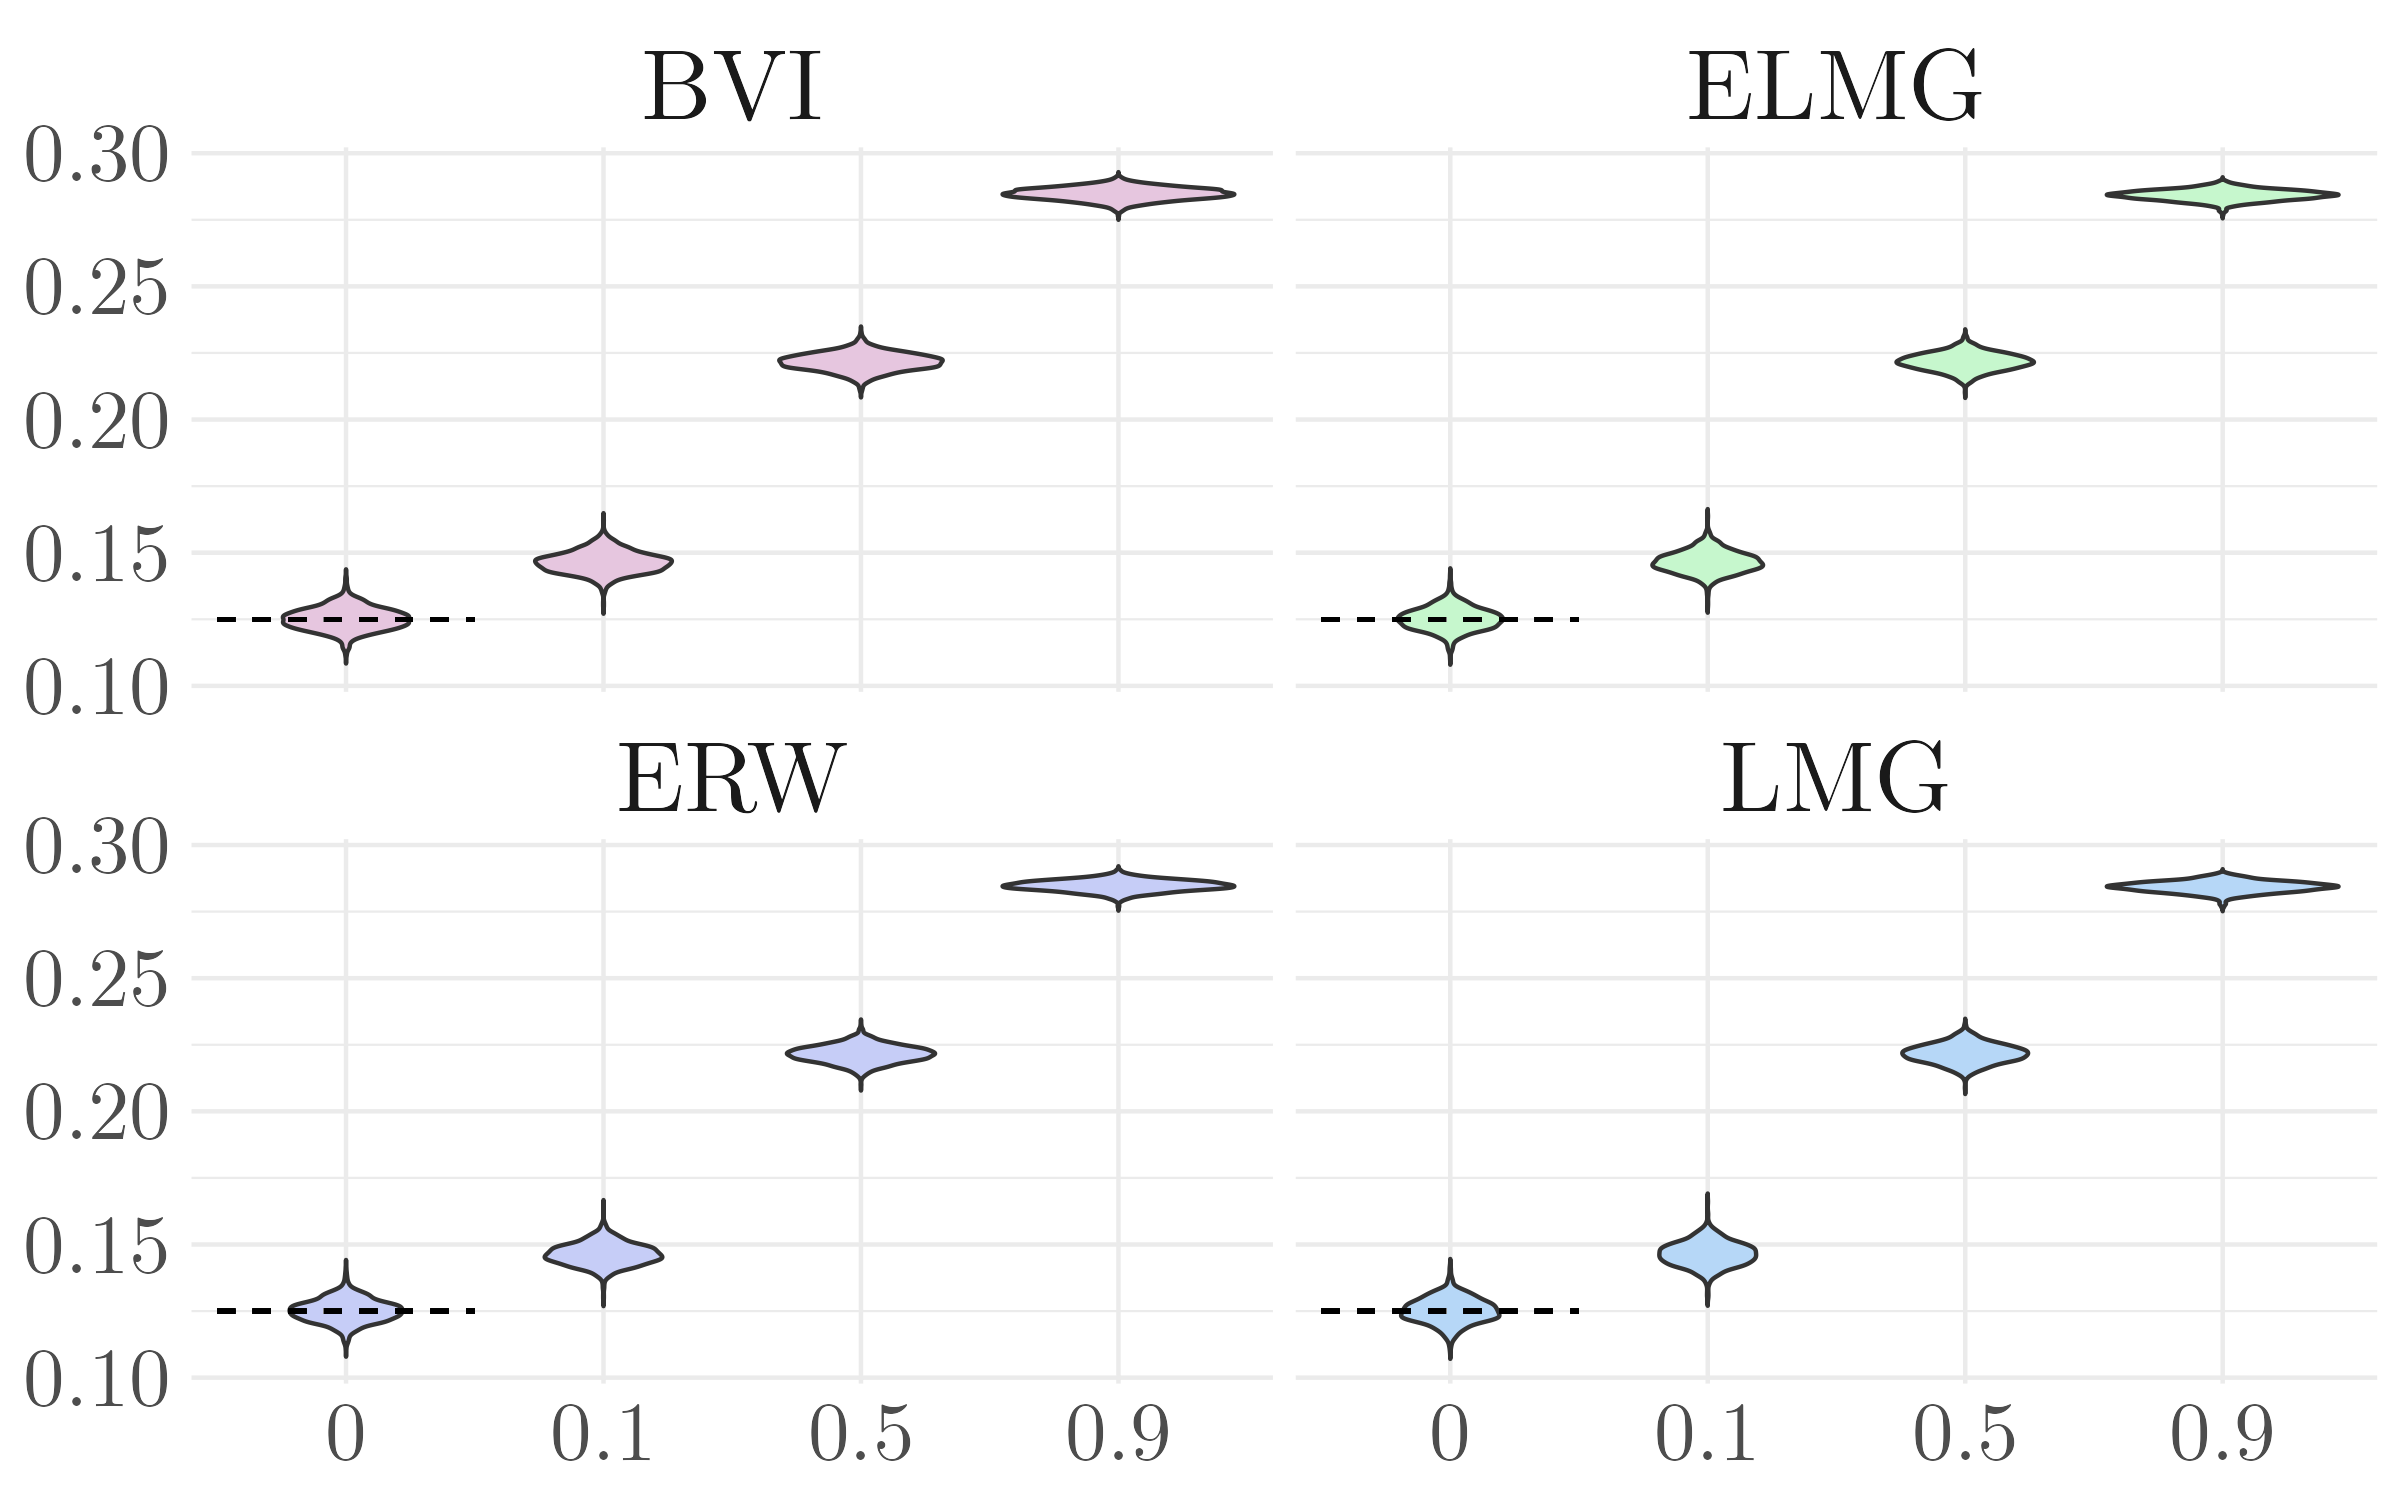
\includegraphics[width=\linewidth]{Figures/ViolinPlots/Variance_V1.png}
    %\caption{Relative importance of $X_1$ as calculated from the four methods.}
    \label{fig:relimp_X1_fig}
  \end{subfigure}
  
  \begin{subfigure}[b]{0.7\linewidth}
    \centering
    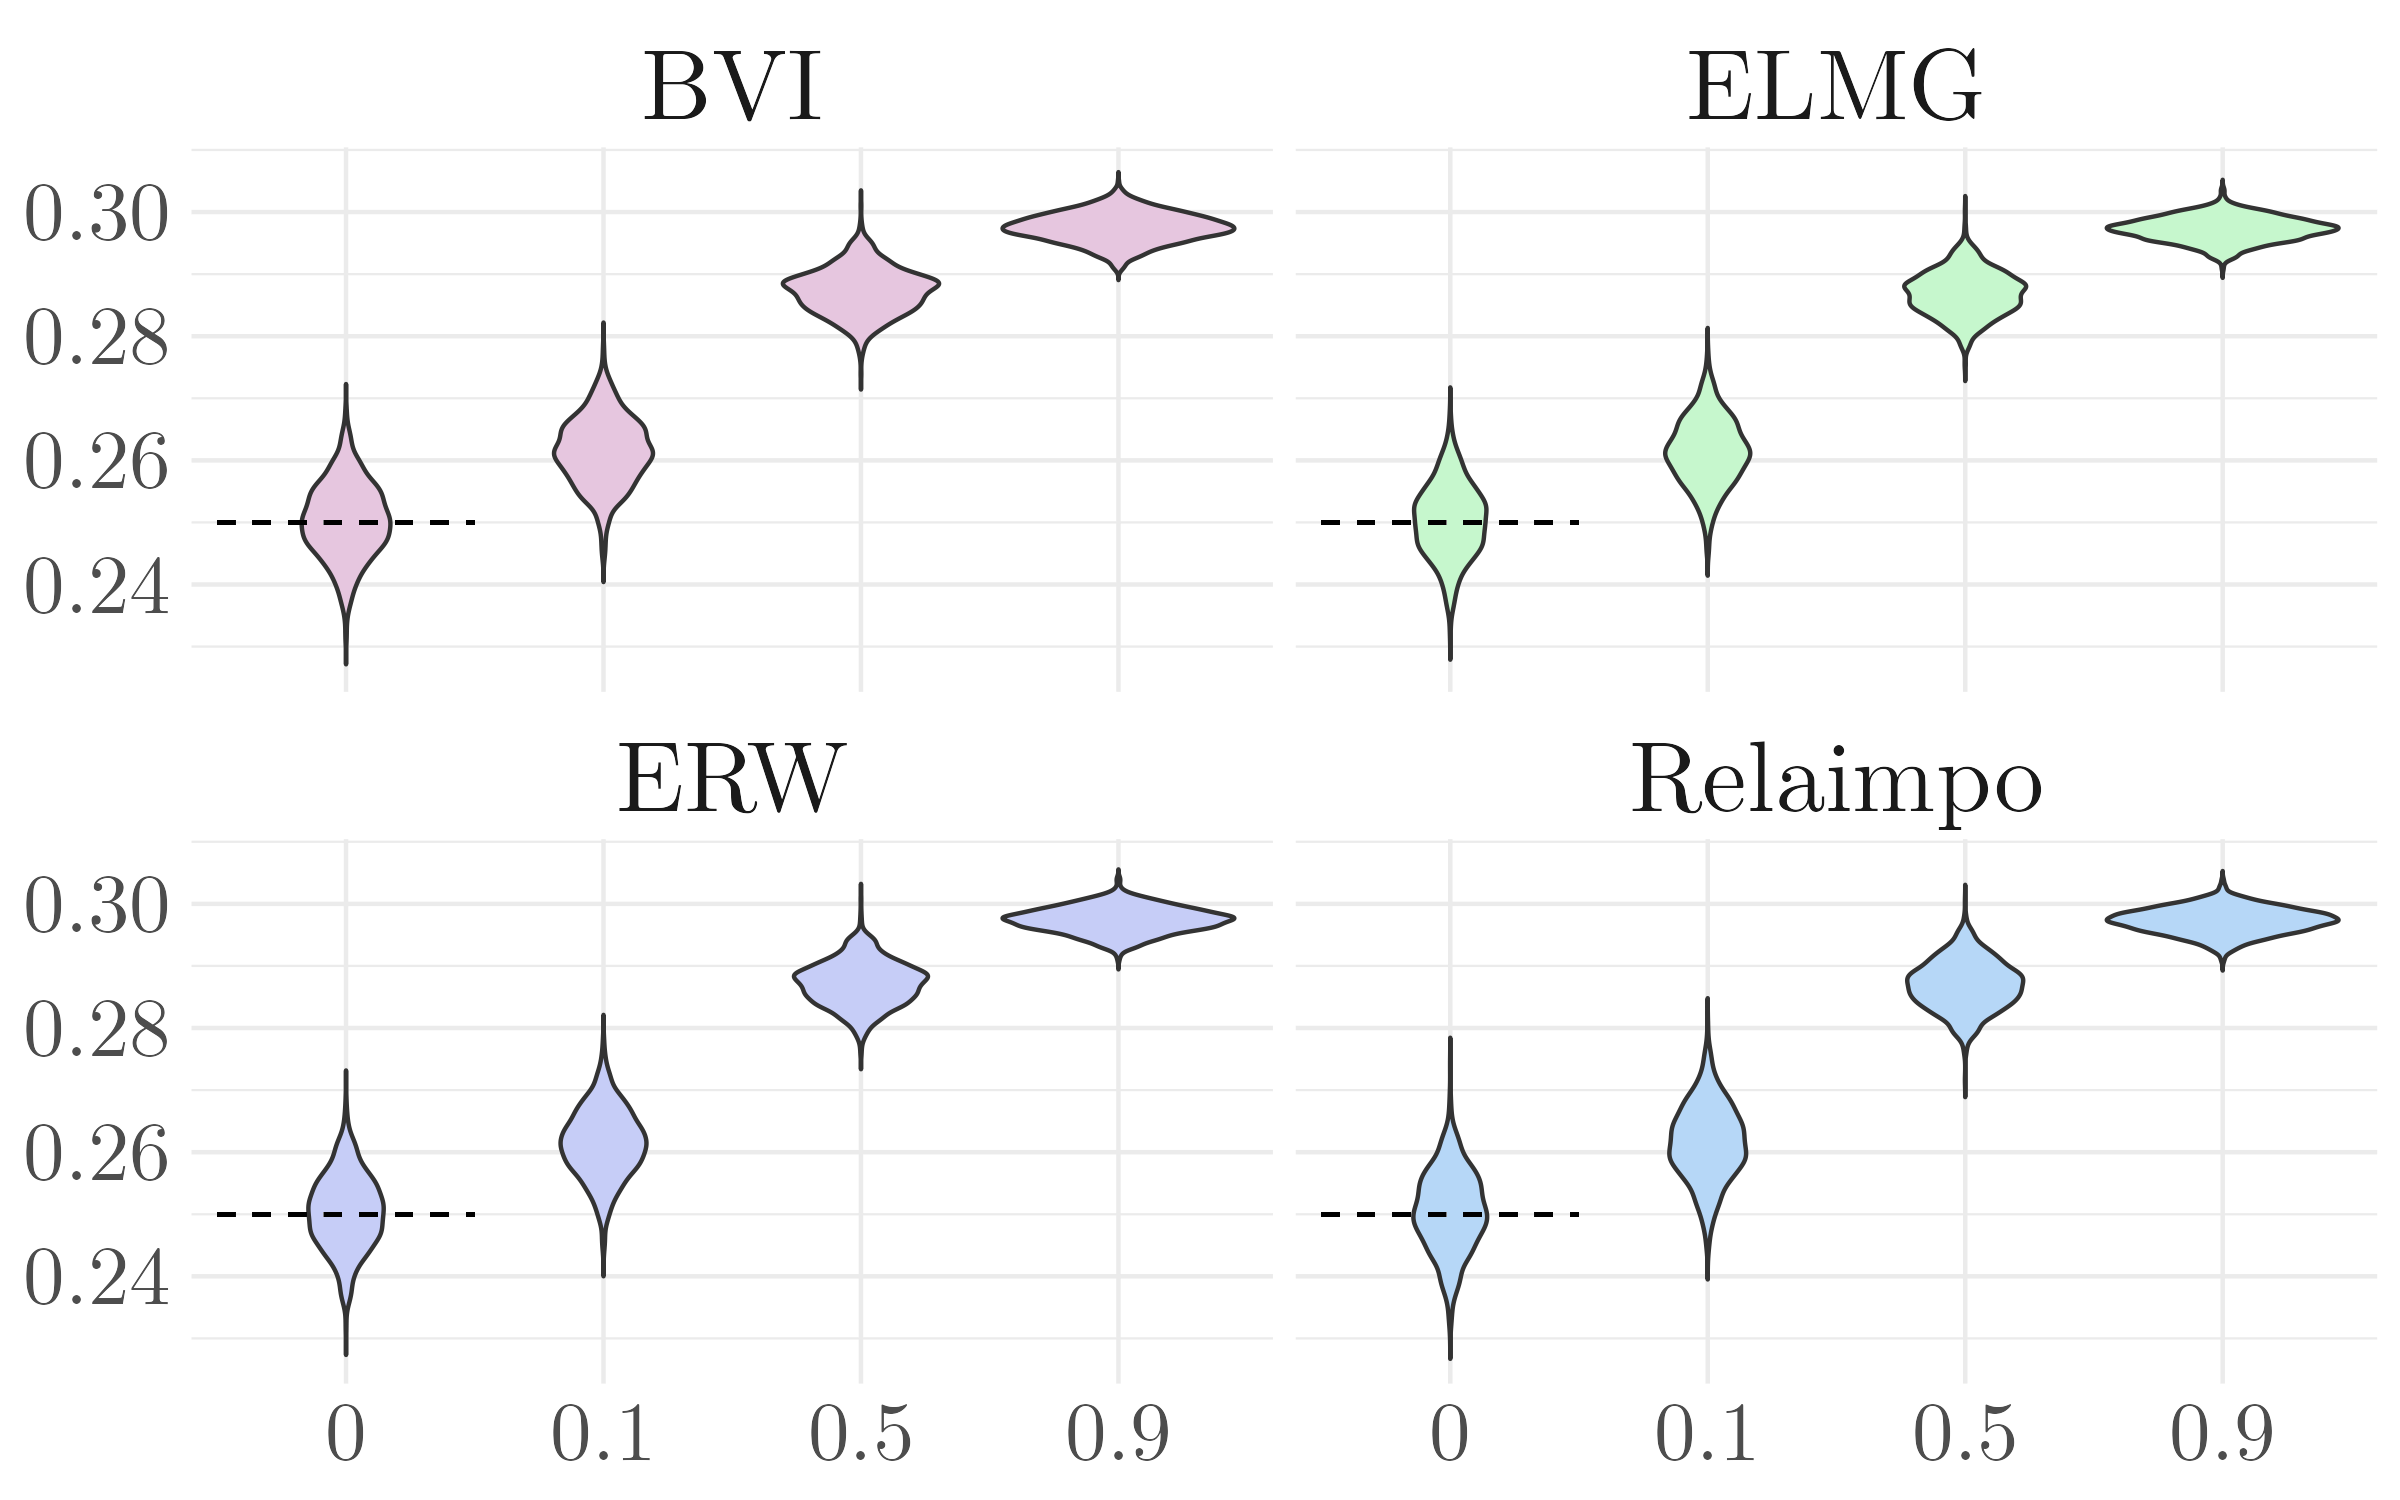
\includegraphics[width=\linewidth]{Figures/ViolinPlots/Variance_V2.png}
   %\caption{Relative importance of $X_2$ as calculated from the four methods.}
    \label{fig:relimp_X2_fig}
  \end{subfigure}
  
  \begin{subfigure}[b]{0.7\linewidth}
    \centering
    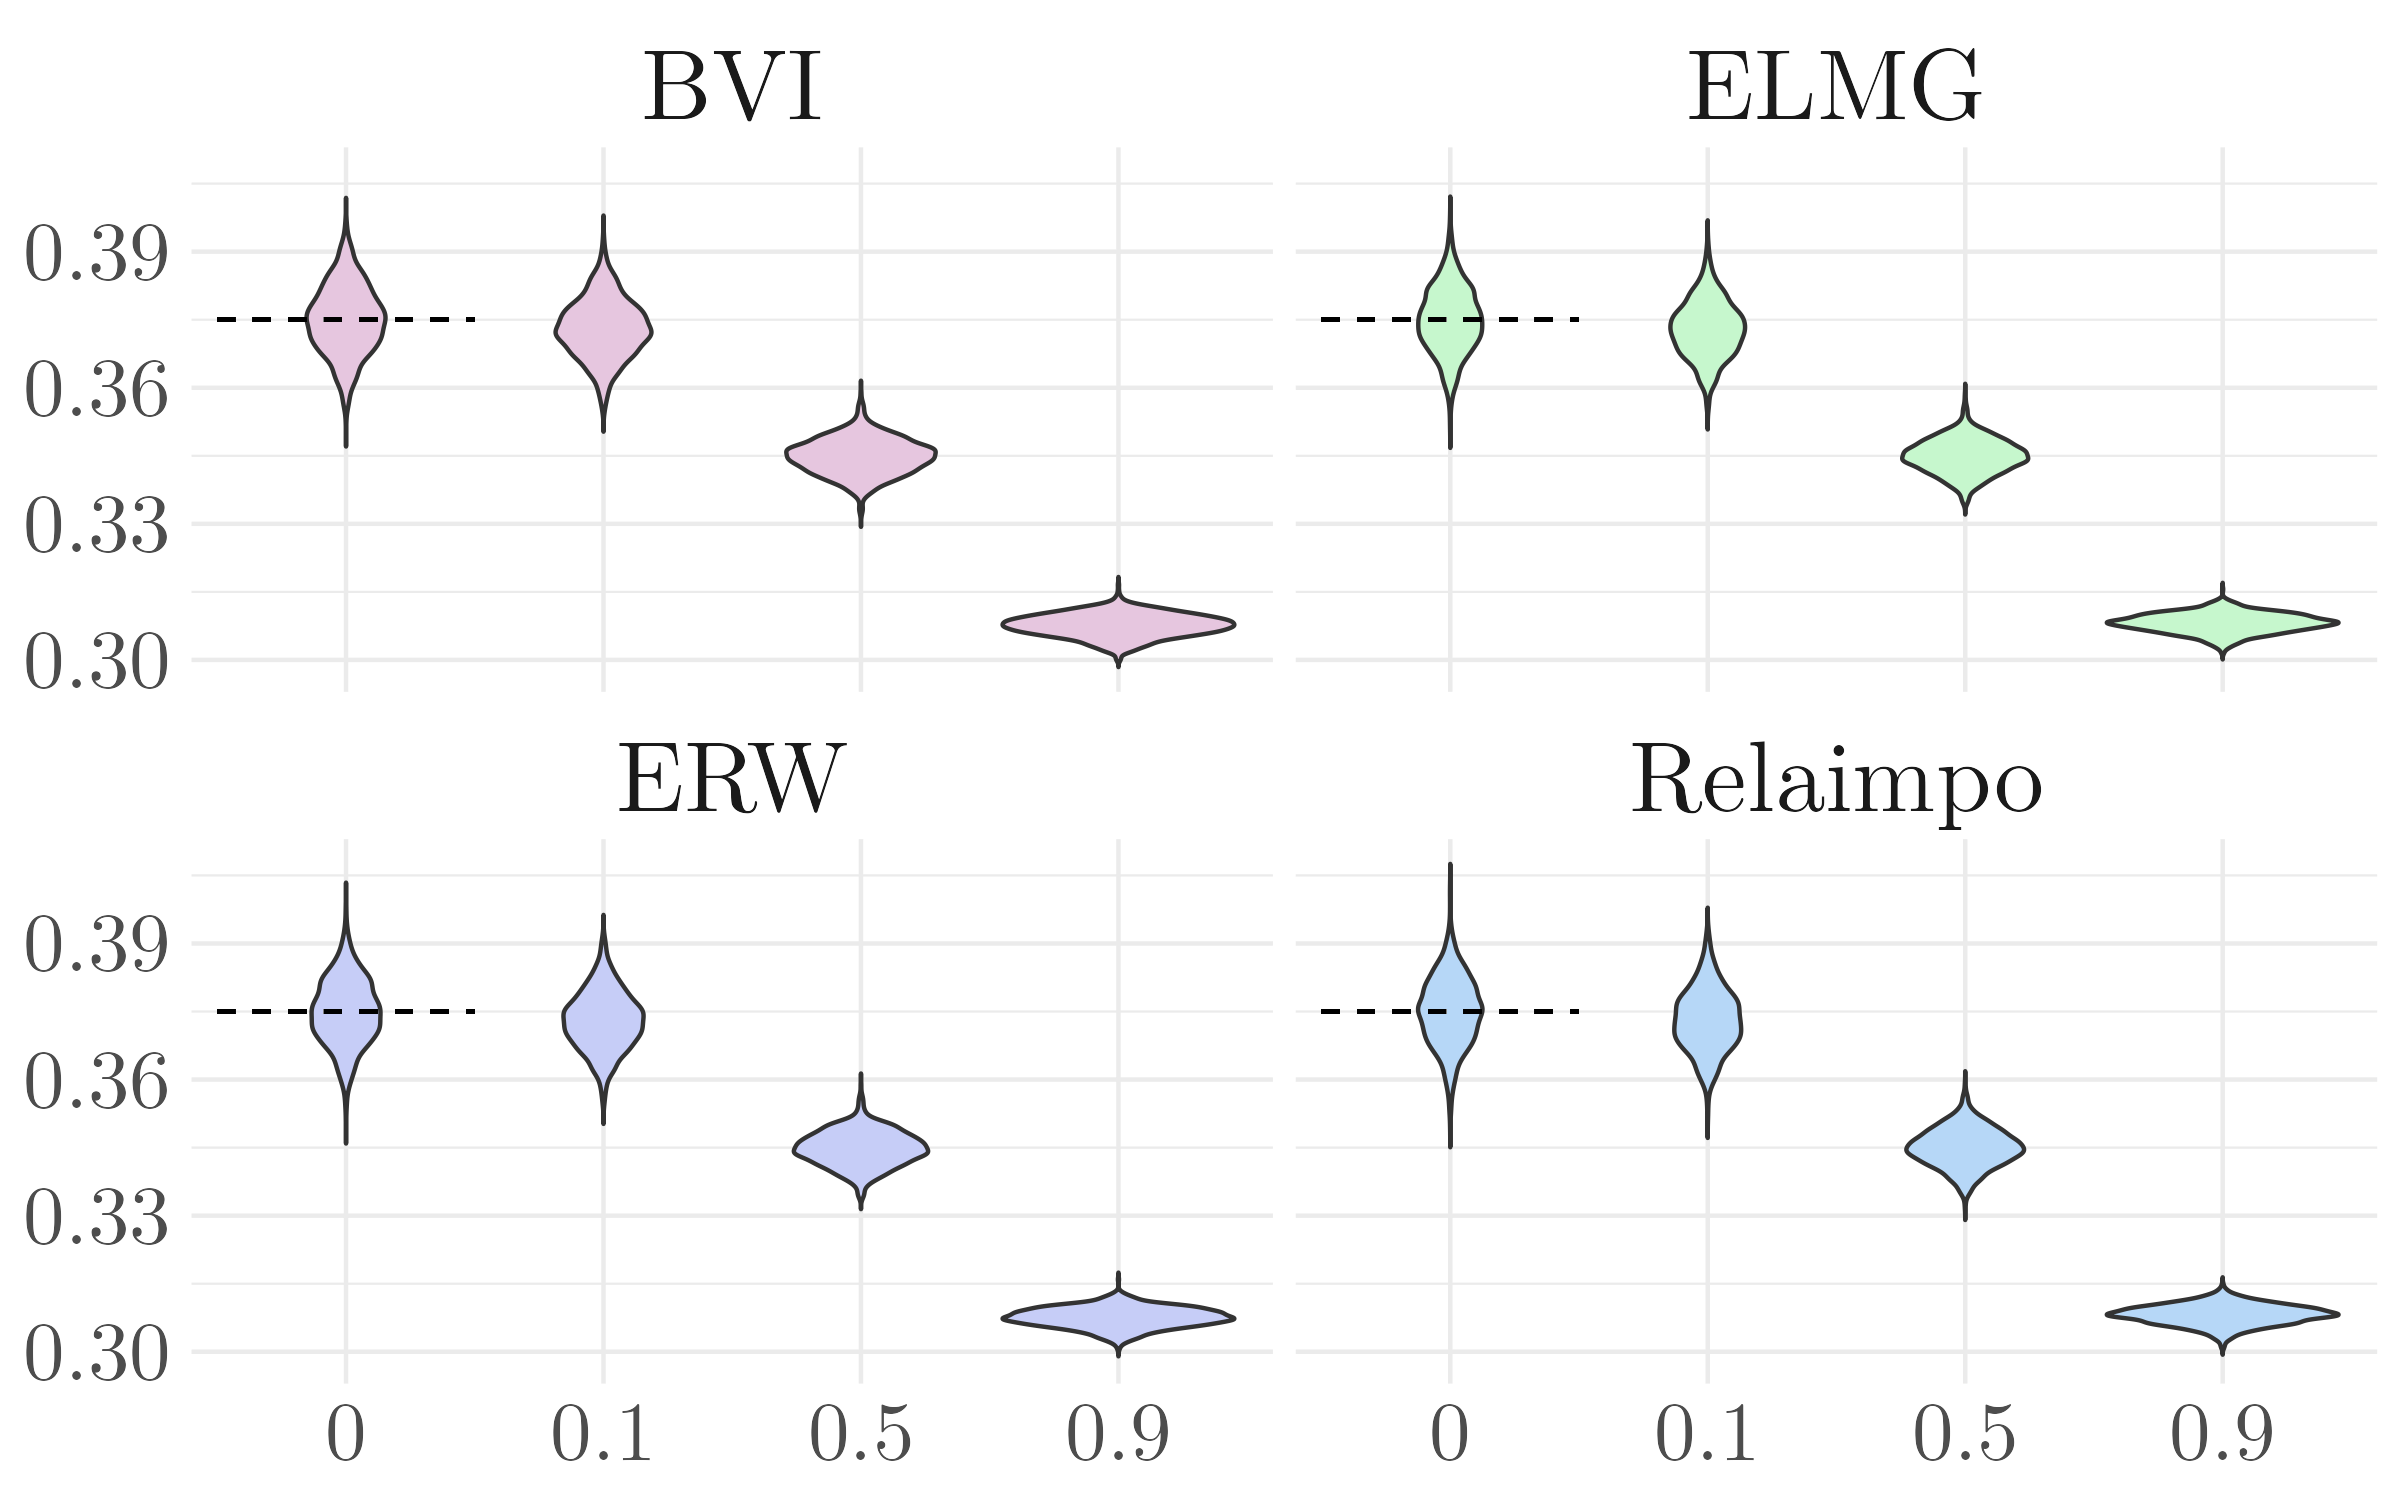
\includegraphics[width=\linewidth]{Figures/ViolinPlots/Variance_V3.png}
    %\caption{Relative importance of $X_3$ as calculated from the four methods.}
    \label{fig:relimp_X3_fig}
  \end{subfigure}
  
  \caption[Relative importance of the fixed effects in Gaussian LMM]{Violin plots for the relative importance of the fixed effects $X_1$ (top), $X_2$ (middle) and $X_3$ (bottom) for different correlation levels displayed along the x-axis, calculated from the ensemble of $N_{\text{sim}}=10^4$ simulated datasets by the BVI, ELMG, ERW, and the Relaimpo methods. The horizontal line displays the theoretically expected importance of each fixed effect in the case of uncorrelated data. For the BVI method, the distributions of posterior means are shown to compare to the distribution of point estimates from the other three methods.}
  \label{fig:relimp_all}
\end{figure}

% \begin{figure}[H]
%   \centering
%     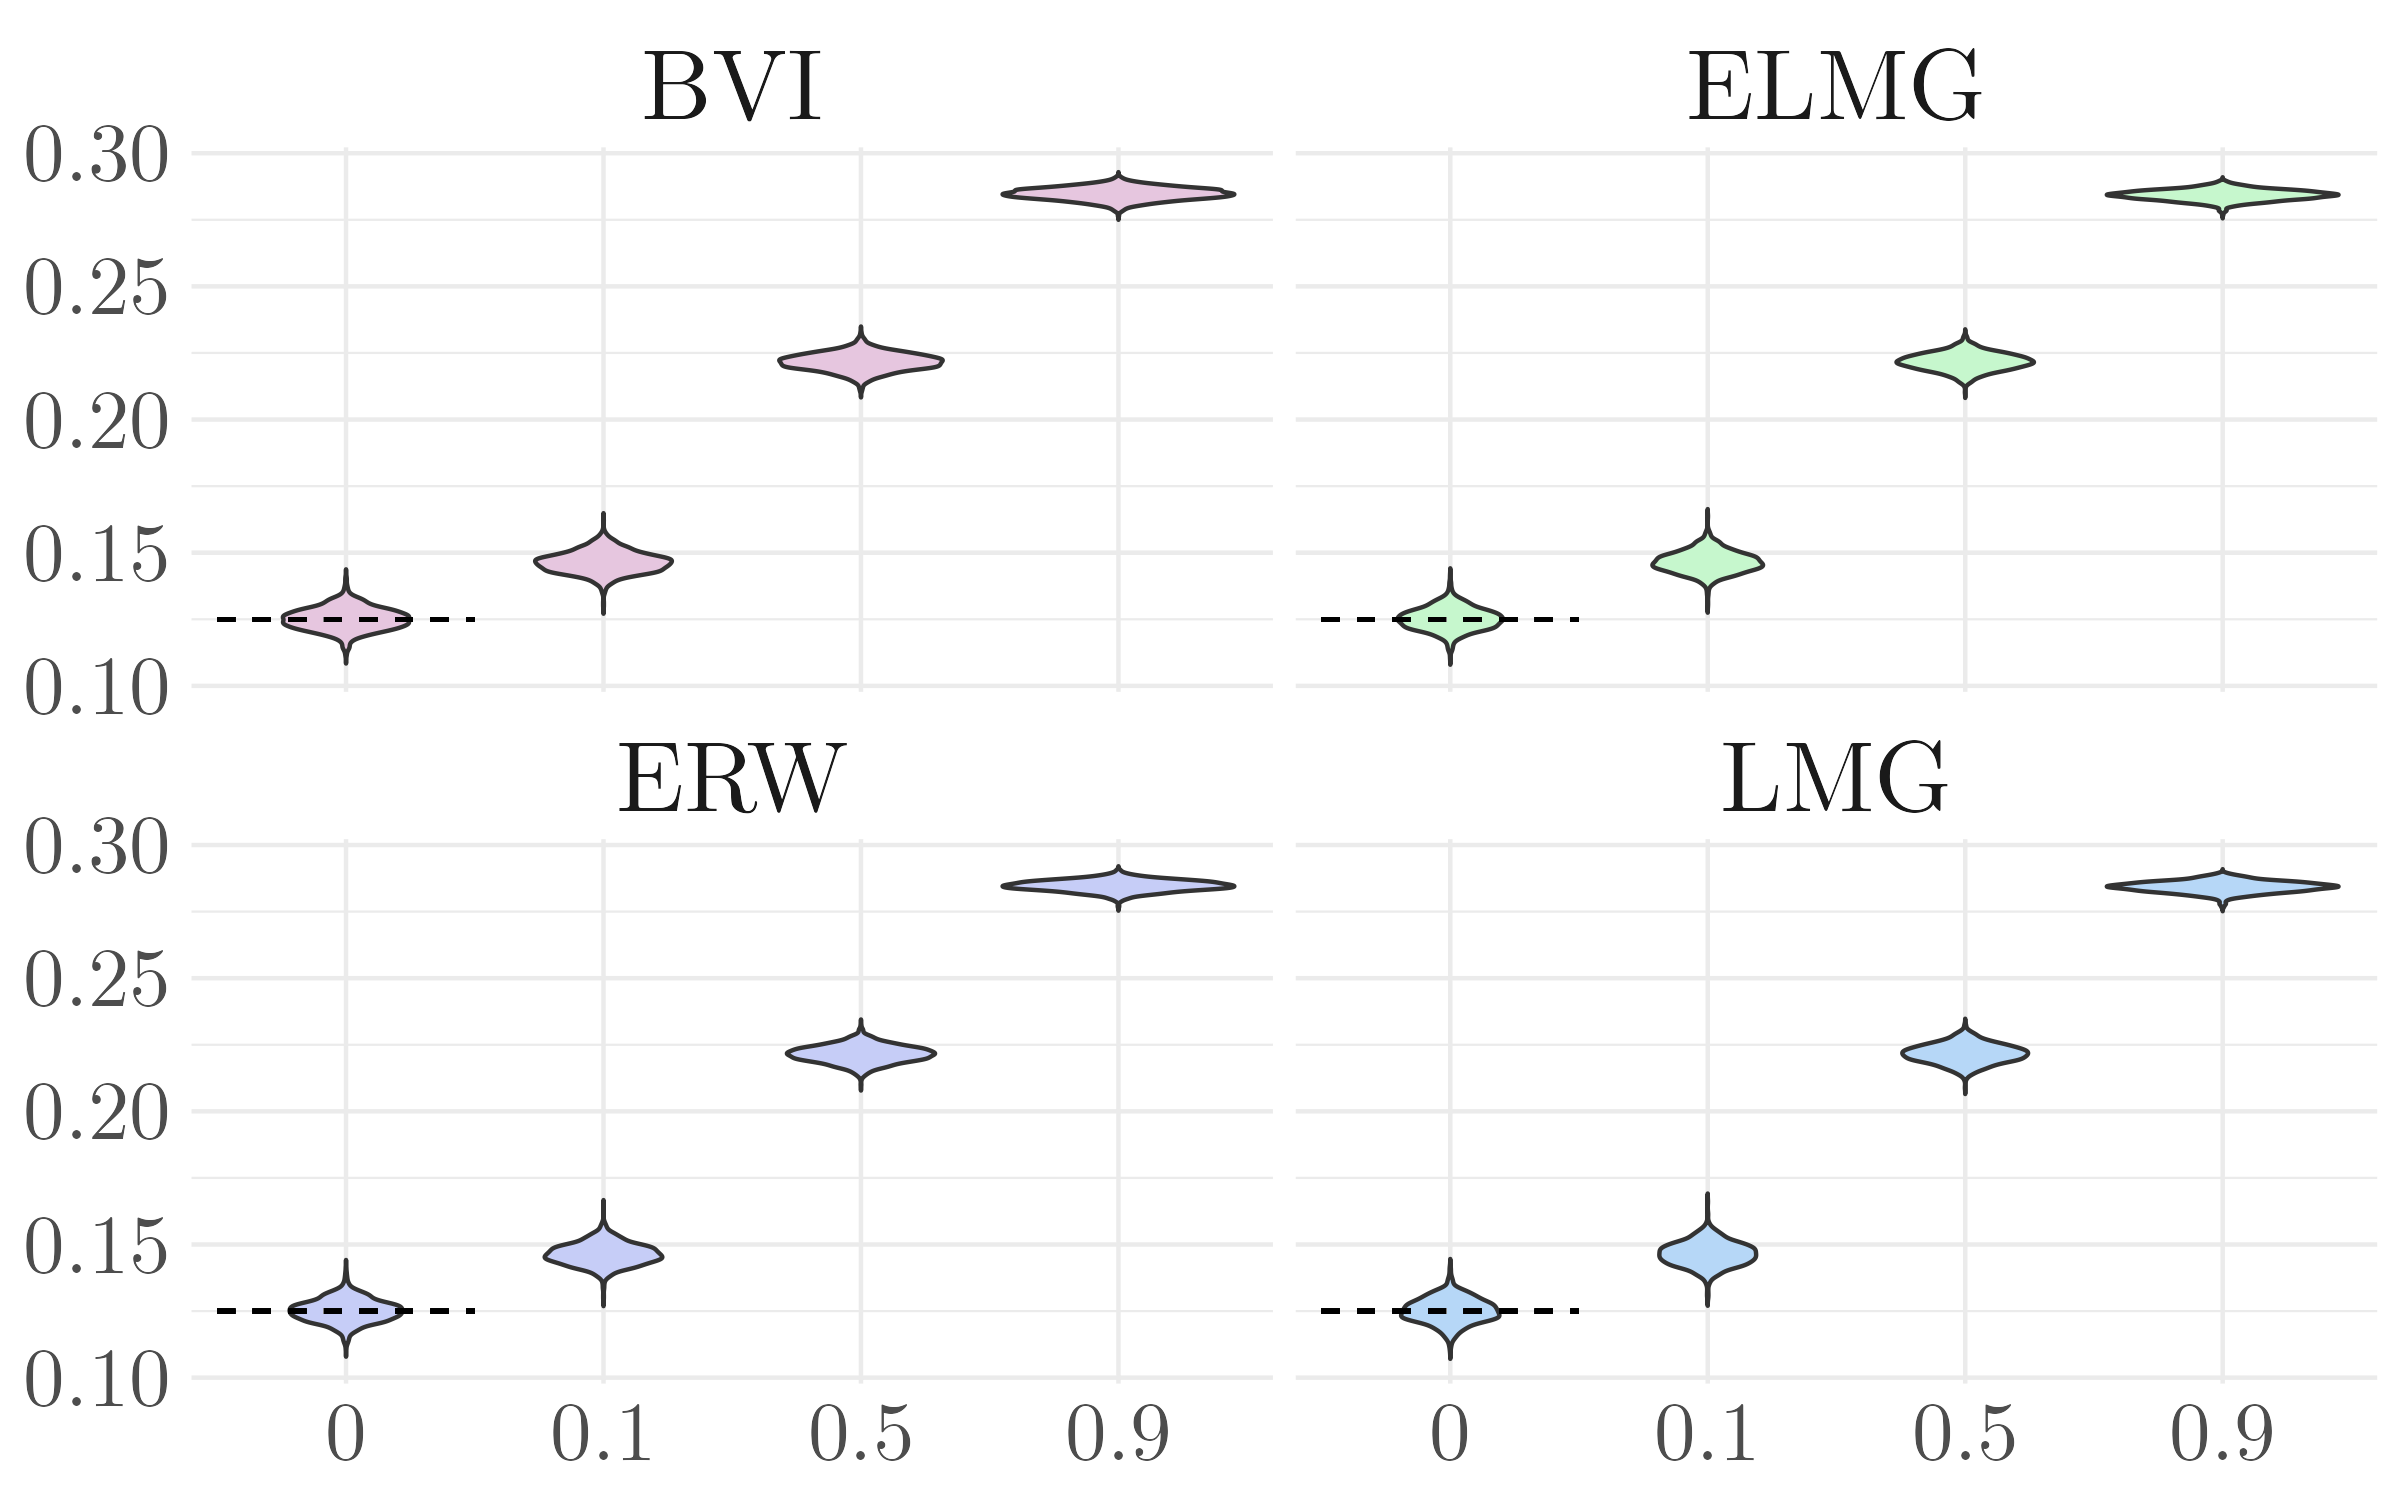
\includegraphics[width=0.7\linewidth]{Figures/ViolinPlots/Variance_V1.png}
%     \caption{Violin plots for the relative importance of the fixed effects $X_1, X_2$ and $X_3$ for different correlation levels calculated from the ensemble of simulated datasets by the BVI, ELMG, ERW and the Relaimpo methods. The standardized regressor coefficients are $\boldsymbol{\beta}=\left(\sqrt{1/8}, \sqrt{2/8}, \sqrt{3/8}\right)$, and the true total model variance is $\sigma^2_{\mathbf{y}}=1$. For the BVI method the distributions of posterior means are shown to compare to the distribution of point estimates from the other three methods. The horizontal line displays the theoretically correct importance of each fixed effect in the case of uncorrelated data. (a) Relative importance of $X_1$ as calculated from the four methods.}
%     \label{fig:relimp_X1}
% \end{figure}
% \begin{figure}[H]\ContinuedFloat
%   \centering
%     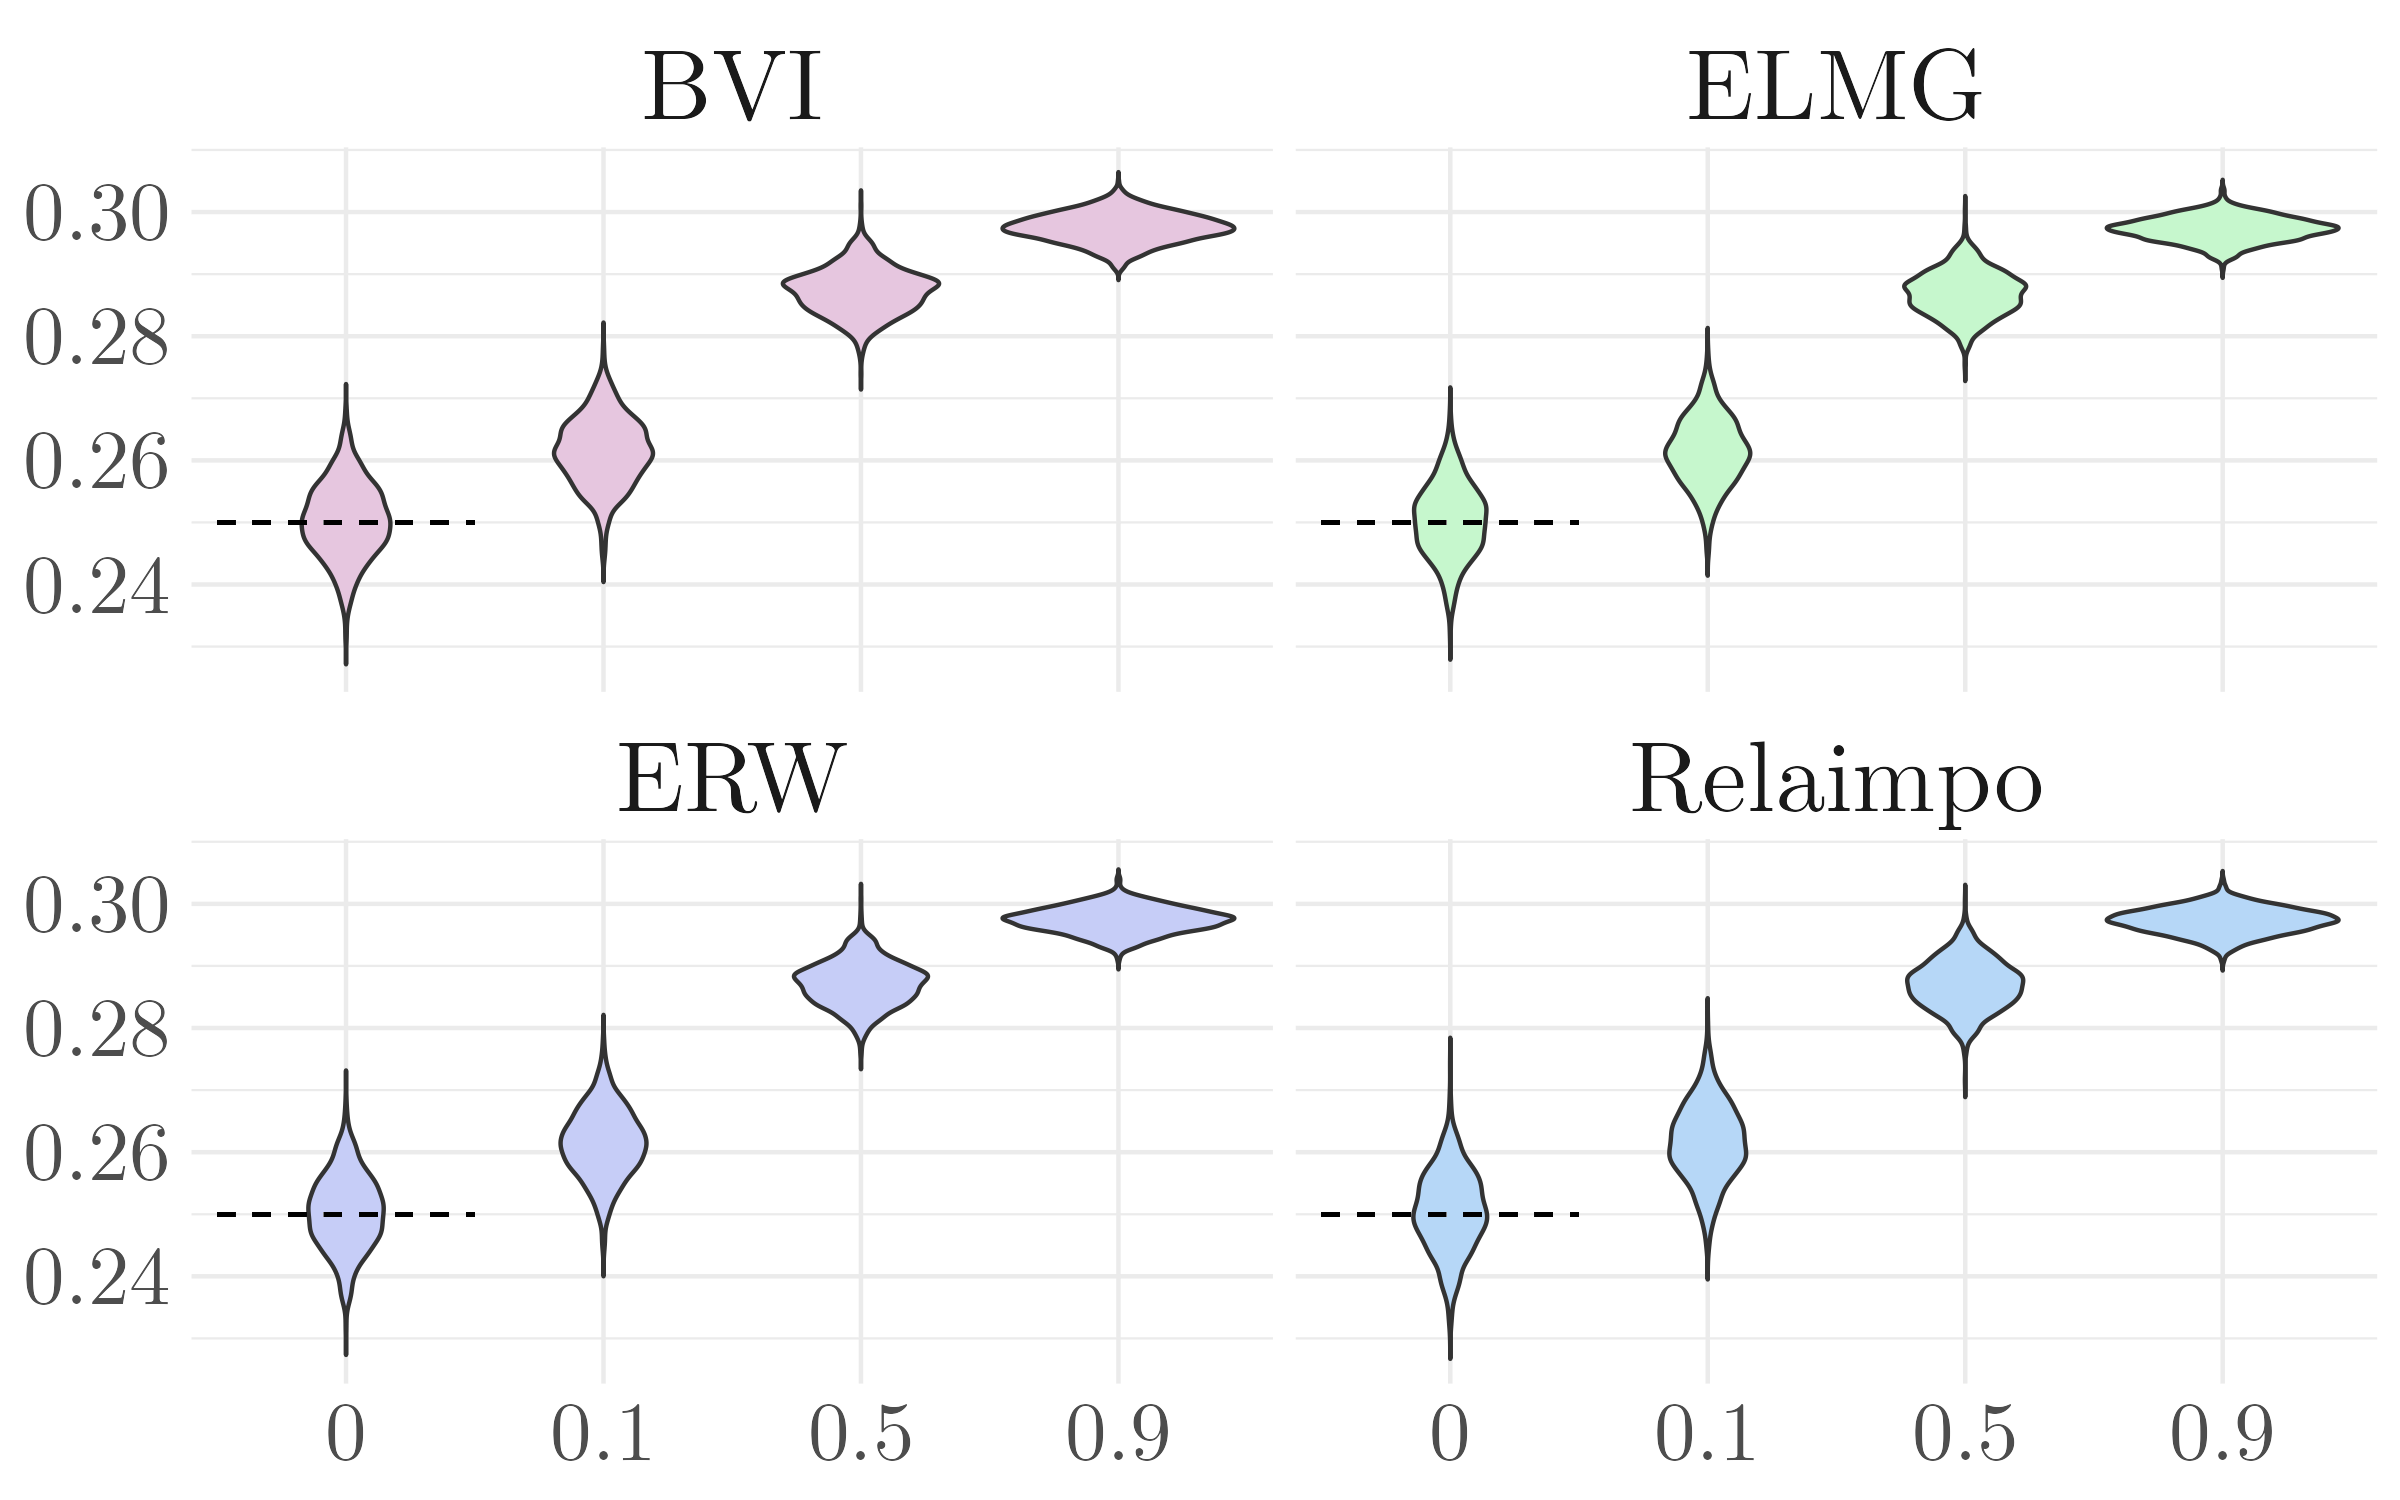
\includegraphics[width=0.7\linewidth]{Figures/ViolinPlots/Variance_V2.png}
%     \caption{(b) Relative importance of $X_2$ as calculated from the four methods.}
%     \label{fig:relimp_X2}
% \end{figure}
% \begin{figure}[H]\ContinuedFloat
%   \centering
%     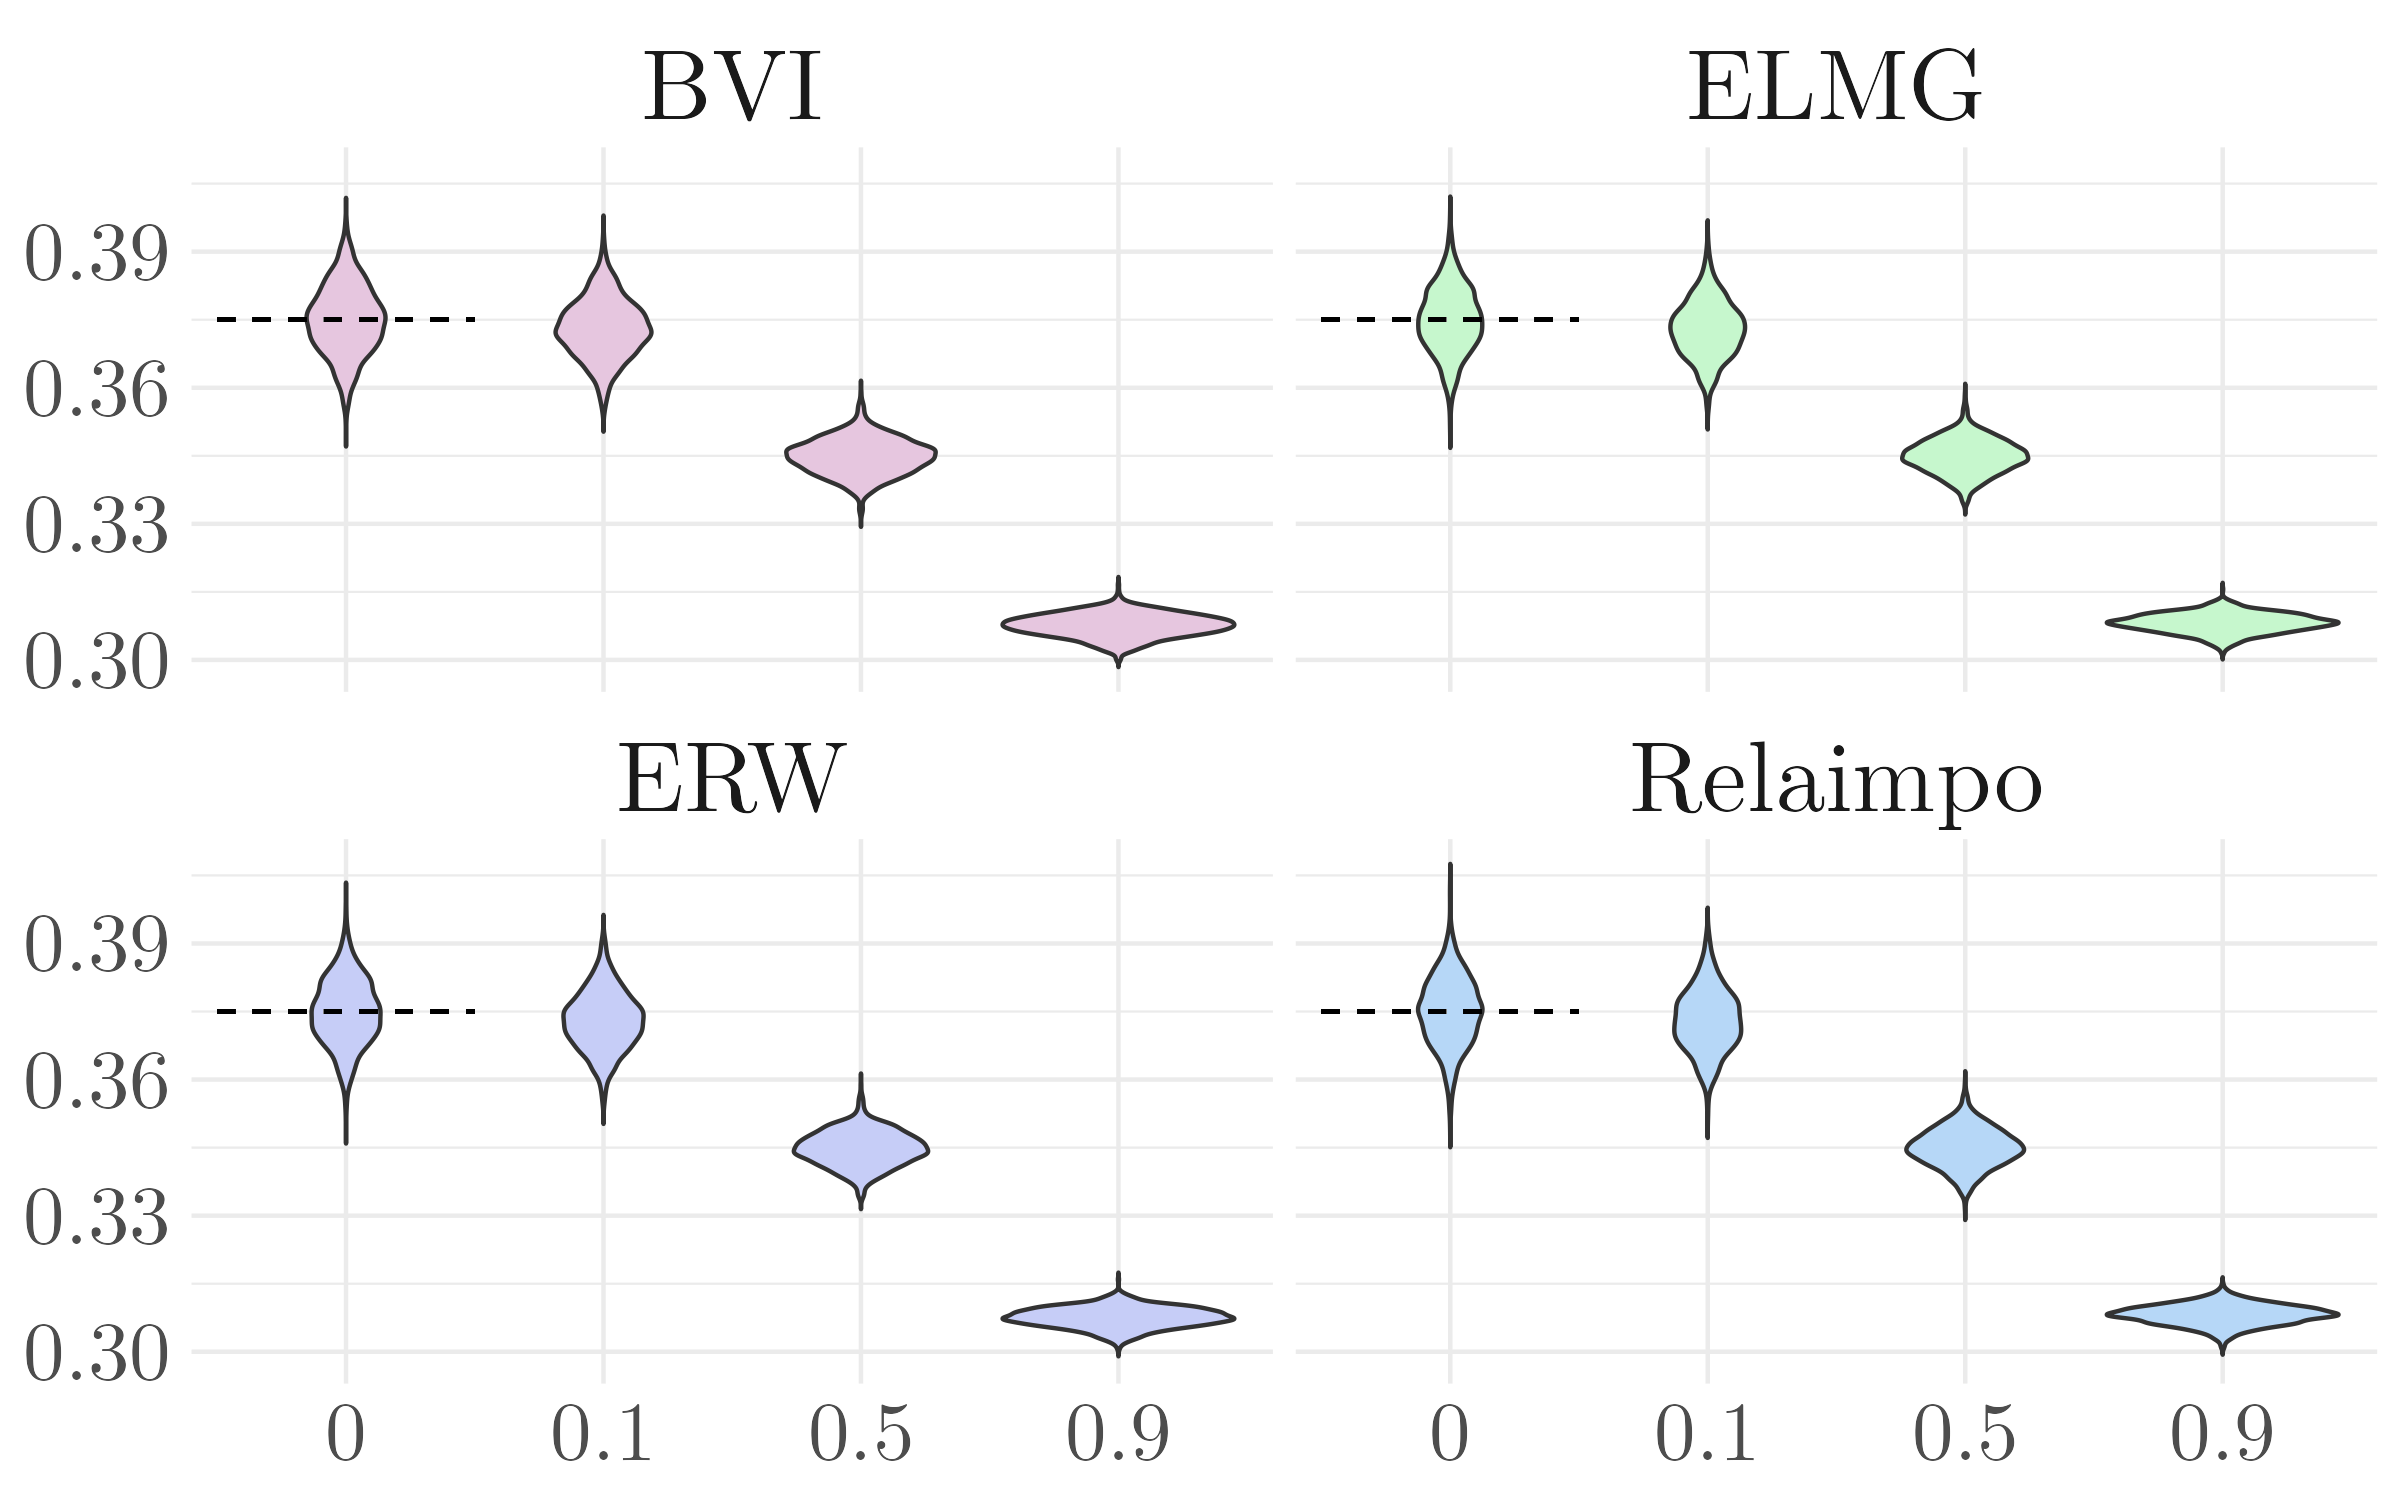
\includegraphics[width=0.7\linewidth]{Figures/ViolinPlots/Variance_V3.png}
%     \caption{(c) Relative importance of $X_3$ as calculated from the four methods.}
%     \label{fig:relimp_X3}
% \end{figure}

\subsection{Random effects}
\label{sec:relimp_random}
Considering a model with one random intercept, we can no longer compare our model with the Relaimpo method, which is only implemented for the linear regression in the Relaimpo R package \citep{gromping_relaimpo}. Therefore, we now compare the BVI method only with the ELMG and ERW methods, which have been extended from the Relaimpo method \citep{matre}.
We display (\Cref{fig:relimp_alpha}) the distribution of the relative importance, or variance, assigned to the random intercept $\boldsymbol{\alpha}$ for different correlation levels. 
The random intercept $\boldsymbol{\alpha}$ follows a univariate normal distribution with mean zero and variance equal to $1$.
As before the horizontal line shows the theoretical relative importance from \eqref{eq:RI_theoretical_simulation} that $\boldsymbol{\alpha}$ has in the model when the fixed effects are uncorrelated.
\newline
\newline
It is apparent that both the location and width of the relative importance distribution of all methods are largely indistinguishable (\Cref{fig:relimp_alpha}). 
The distributions take on a moderately smaller value when $\rho=0.1$ and the location of the estimates is further decreased for $\rho=0.5$ and $\rho=0.9$. 
For the latter correlation level, the distributions are located around a value that is less than half of the value of the centering when the fixed effects are uncorrelated. 
To re-emphasize, this is both expected and desirable since the increase in response variance comes solely from the correlation of fixed effects, so the random effects now contribute to explain a smaller proportion of the variance, \textit{i.e.} the importance is lower.
\begin{figure}[ht]
  \centering
  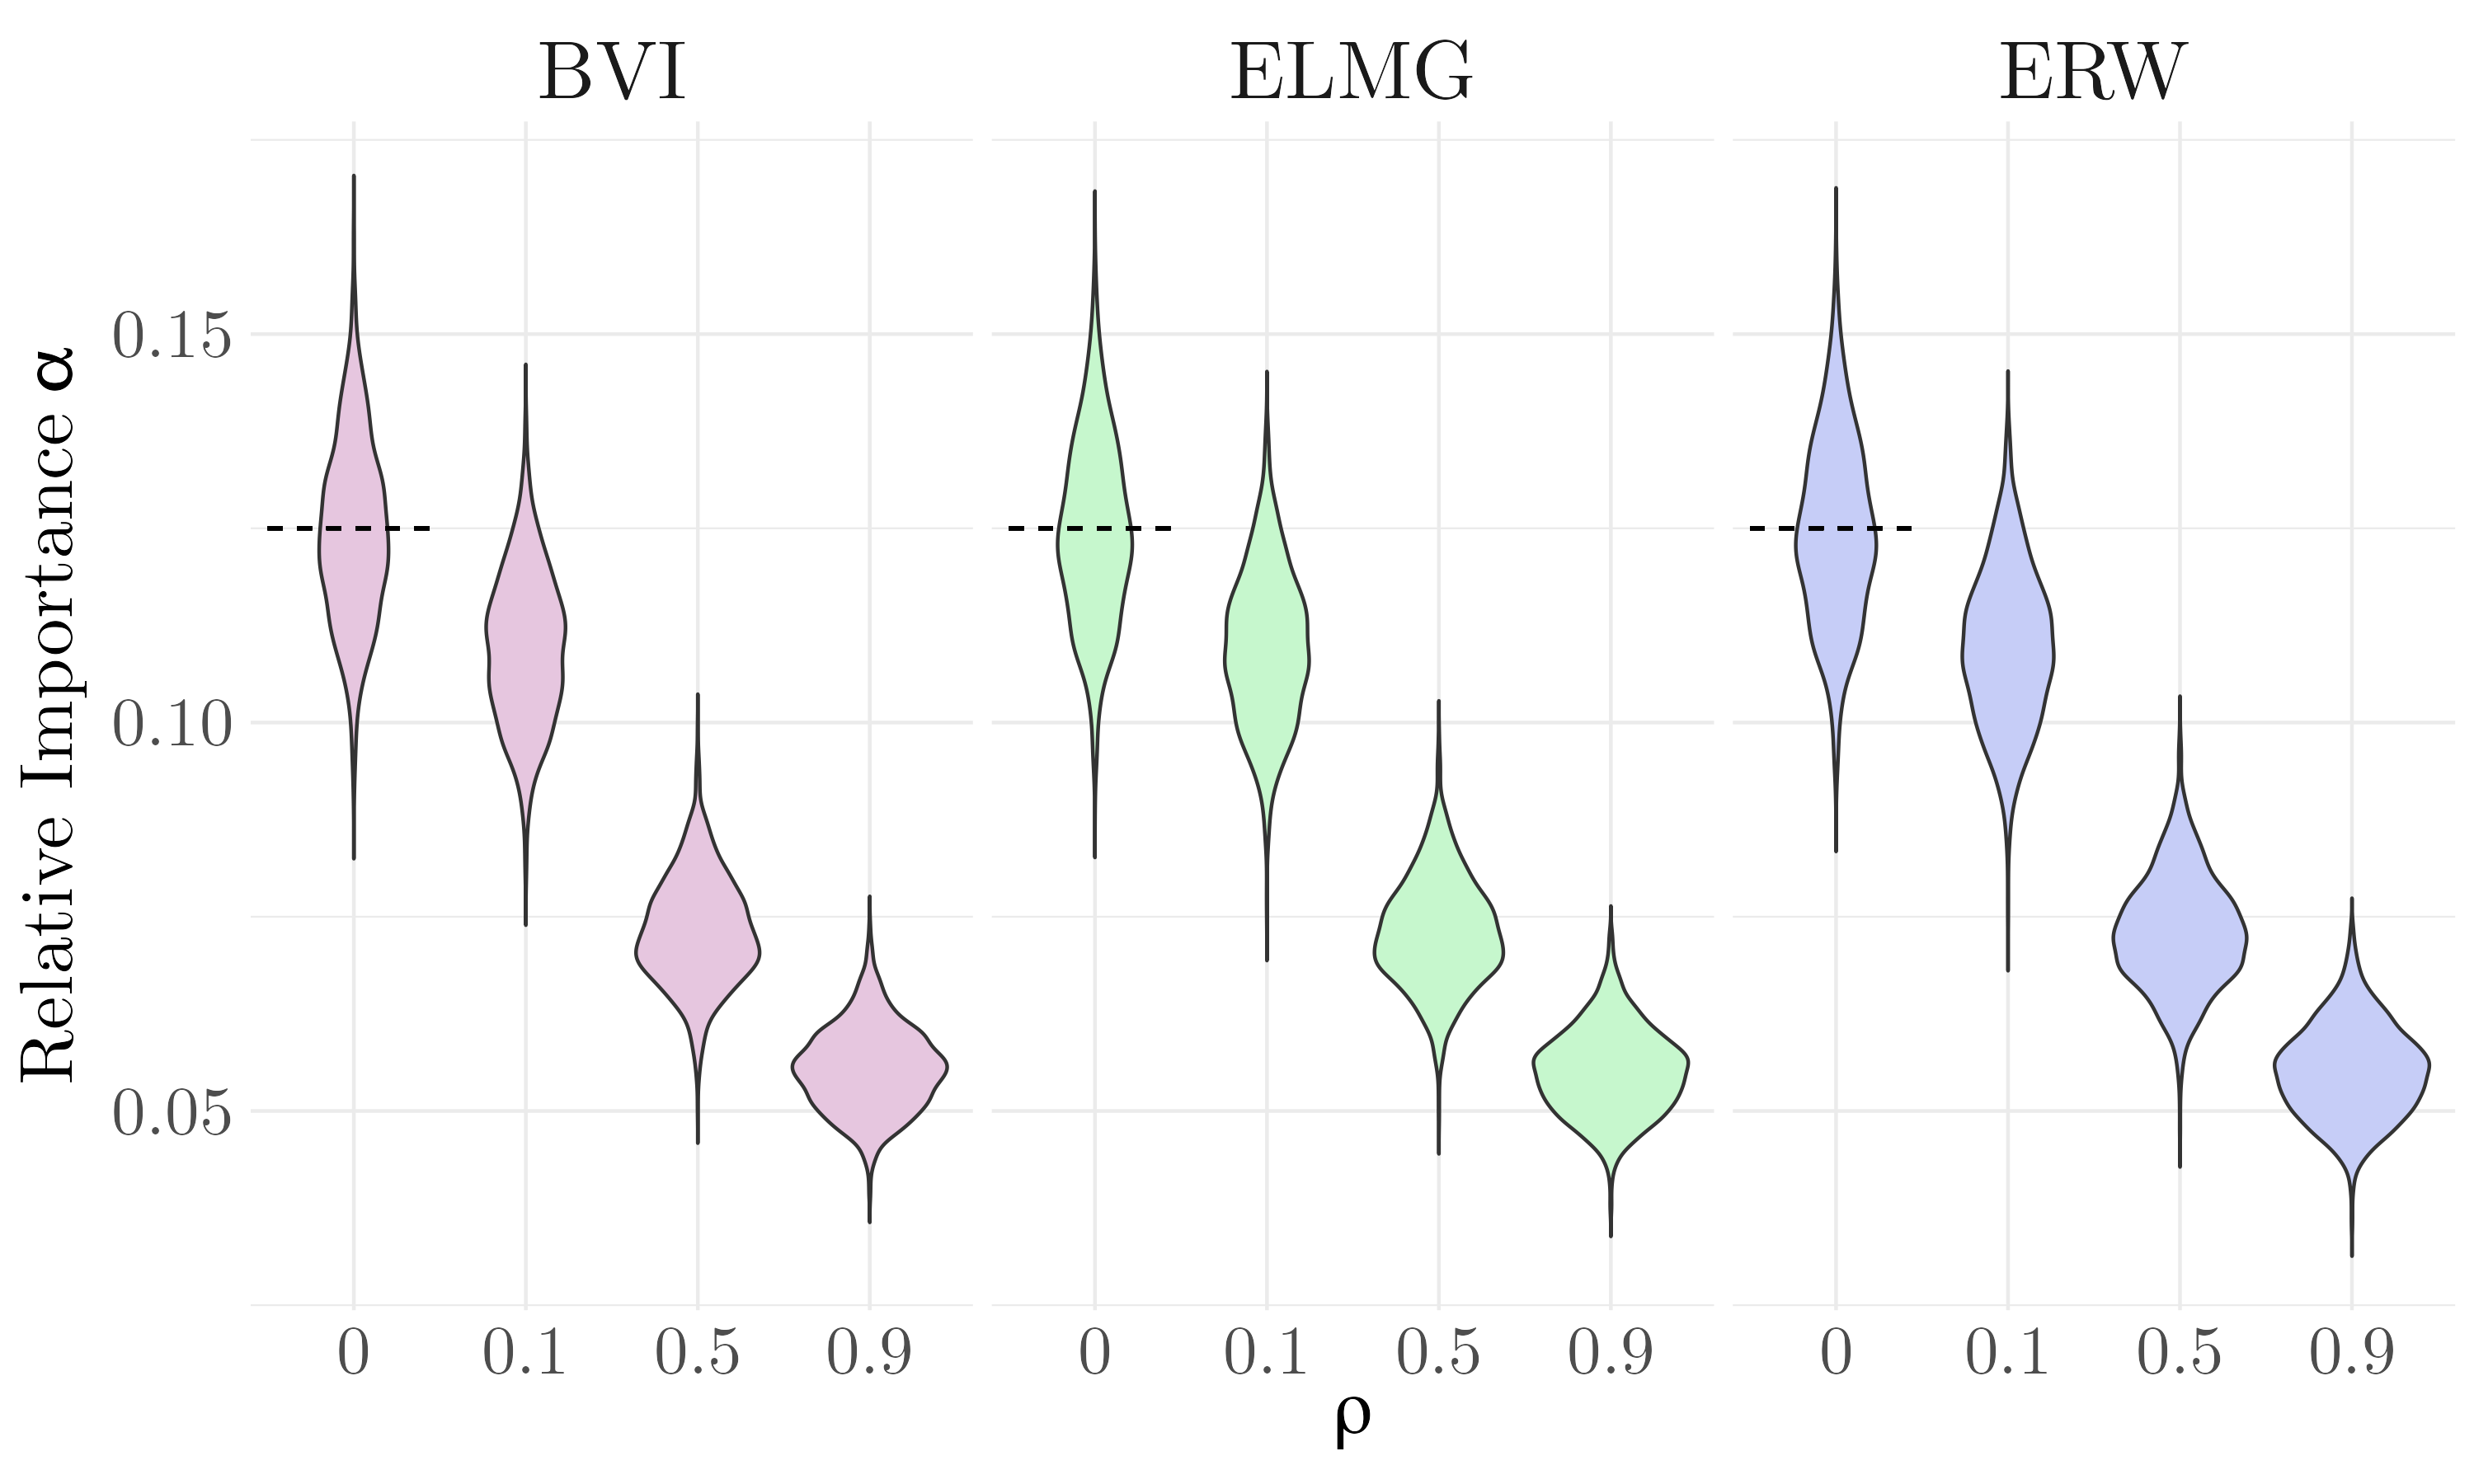
\includegraphics[width=0.7\linewidth]{Figures/ViolinPlots/Variance_gamma.png}
  \caption[Relative importance of the random effect $\boldsymbol{\alpha}$ in Gaussian LMM]{Violin plots for the relative importance of the random effect $\boldsymbol{\alpha}$, that is, $\hat{\sigma}^2_{\alpha}$ for different correlation levels displayed along the x-axis, calculated from the ensemble of $N_{\sim=10^4}$ simulated datasets by the BVI, ELMG and the ERW method. For the BVI method the distributions of posterior means of the marginal distribution of $\hat{\sigma}^2_{\alpha}$ are shown to compare to the point estimates of the other two methods. The horizontal line displays the theoretically expected importance $\sigma^2_{\alpha}$ of the random effect in the case of uncorrelated data.}
  \label{fig:relimp_alpha}
\end{figure}

\subsection{\texorpdfstring{$R^2$}{Lg} estimates}
\label{sec:R2} 
As a useful by-product from the previous results we can get the total variances explained by our model (\Cref{fig:total_variance}).
The marginal variance explained, $R^2_{\text{marg}}$, is the variance explained by the fixed effects, and we get results for all four methods, including Relaimpo.
Below, the marginal variance explained, and the total conditional variance explained, $R^2_{\text{cond}}$, is displayed. 
This is the variance given all the fixed effects and the random effect.
To complement the conditional and marginal variances explained, a horizontal line is drawn for each correlation level corresponding to the theoretically expected variance explained, found in \Cref{table:2}, for the correlation level. 
\newline
\newline
We see that the four methods produce very similar results of $R^2_{\text{marg}}$ for the fixed effects across all correlation values, albeit a slightly larger width for the BVI method can be seen.
When considering the conditional variance $R^2_{\text{cond}}$, the dispersion of the BVI method is strikingly larger compared to the other methods. 
It is not immediately clear why, but it could be a result of the relatively large dispersion of the estimated posterior marginal variance of $\boldsymbol{\alpha}$.
Both the marginal and the conditional variance are centered around the theoretically correct value with some variability, particularly visible for conditional variance of the BVI method. 
The centering of the distributions for both the marginal and conditional variances resemble each other for all methods, regardless of correlation level.
\begin{figure}[H]
  \centering
  % First row
  \subfloat{
    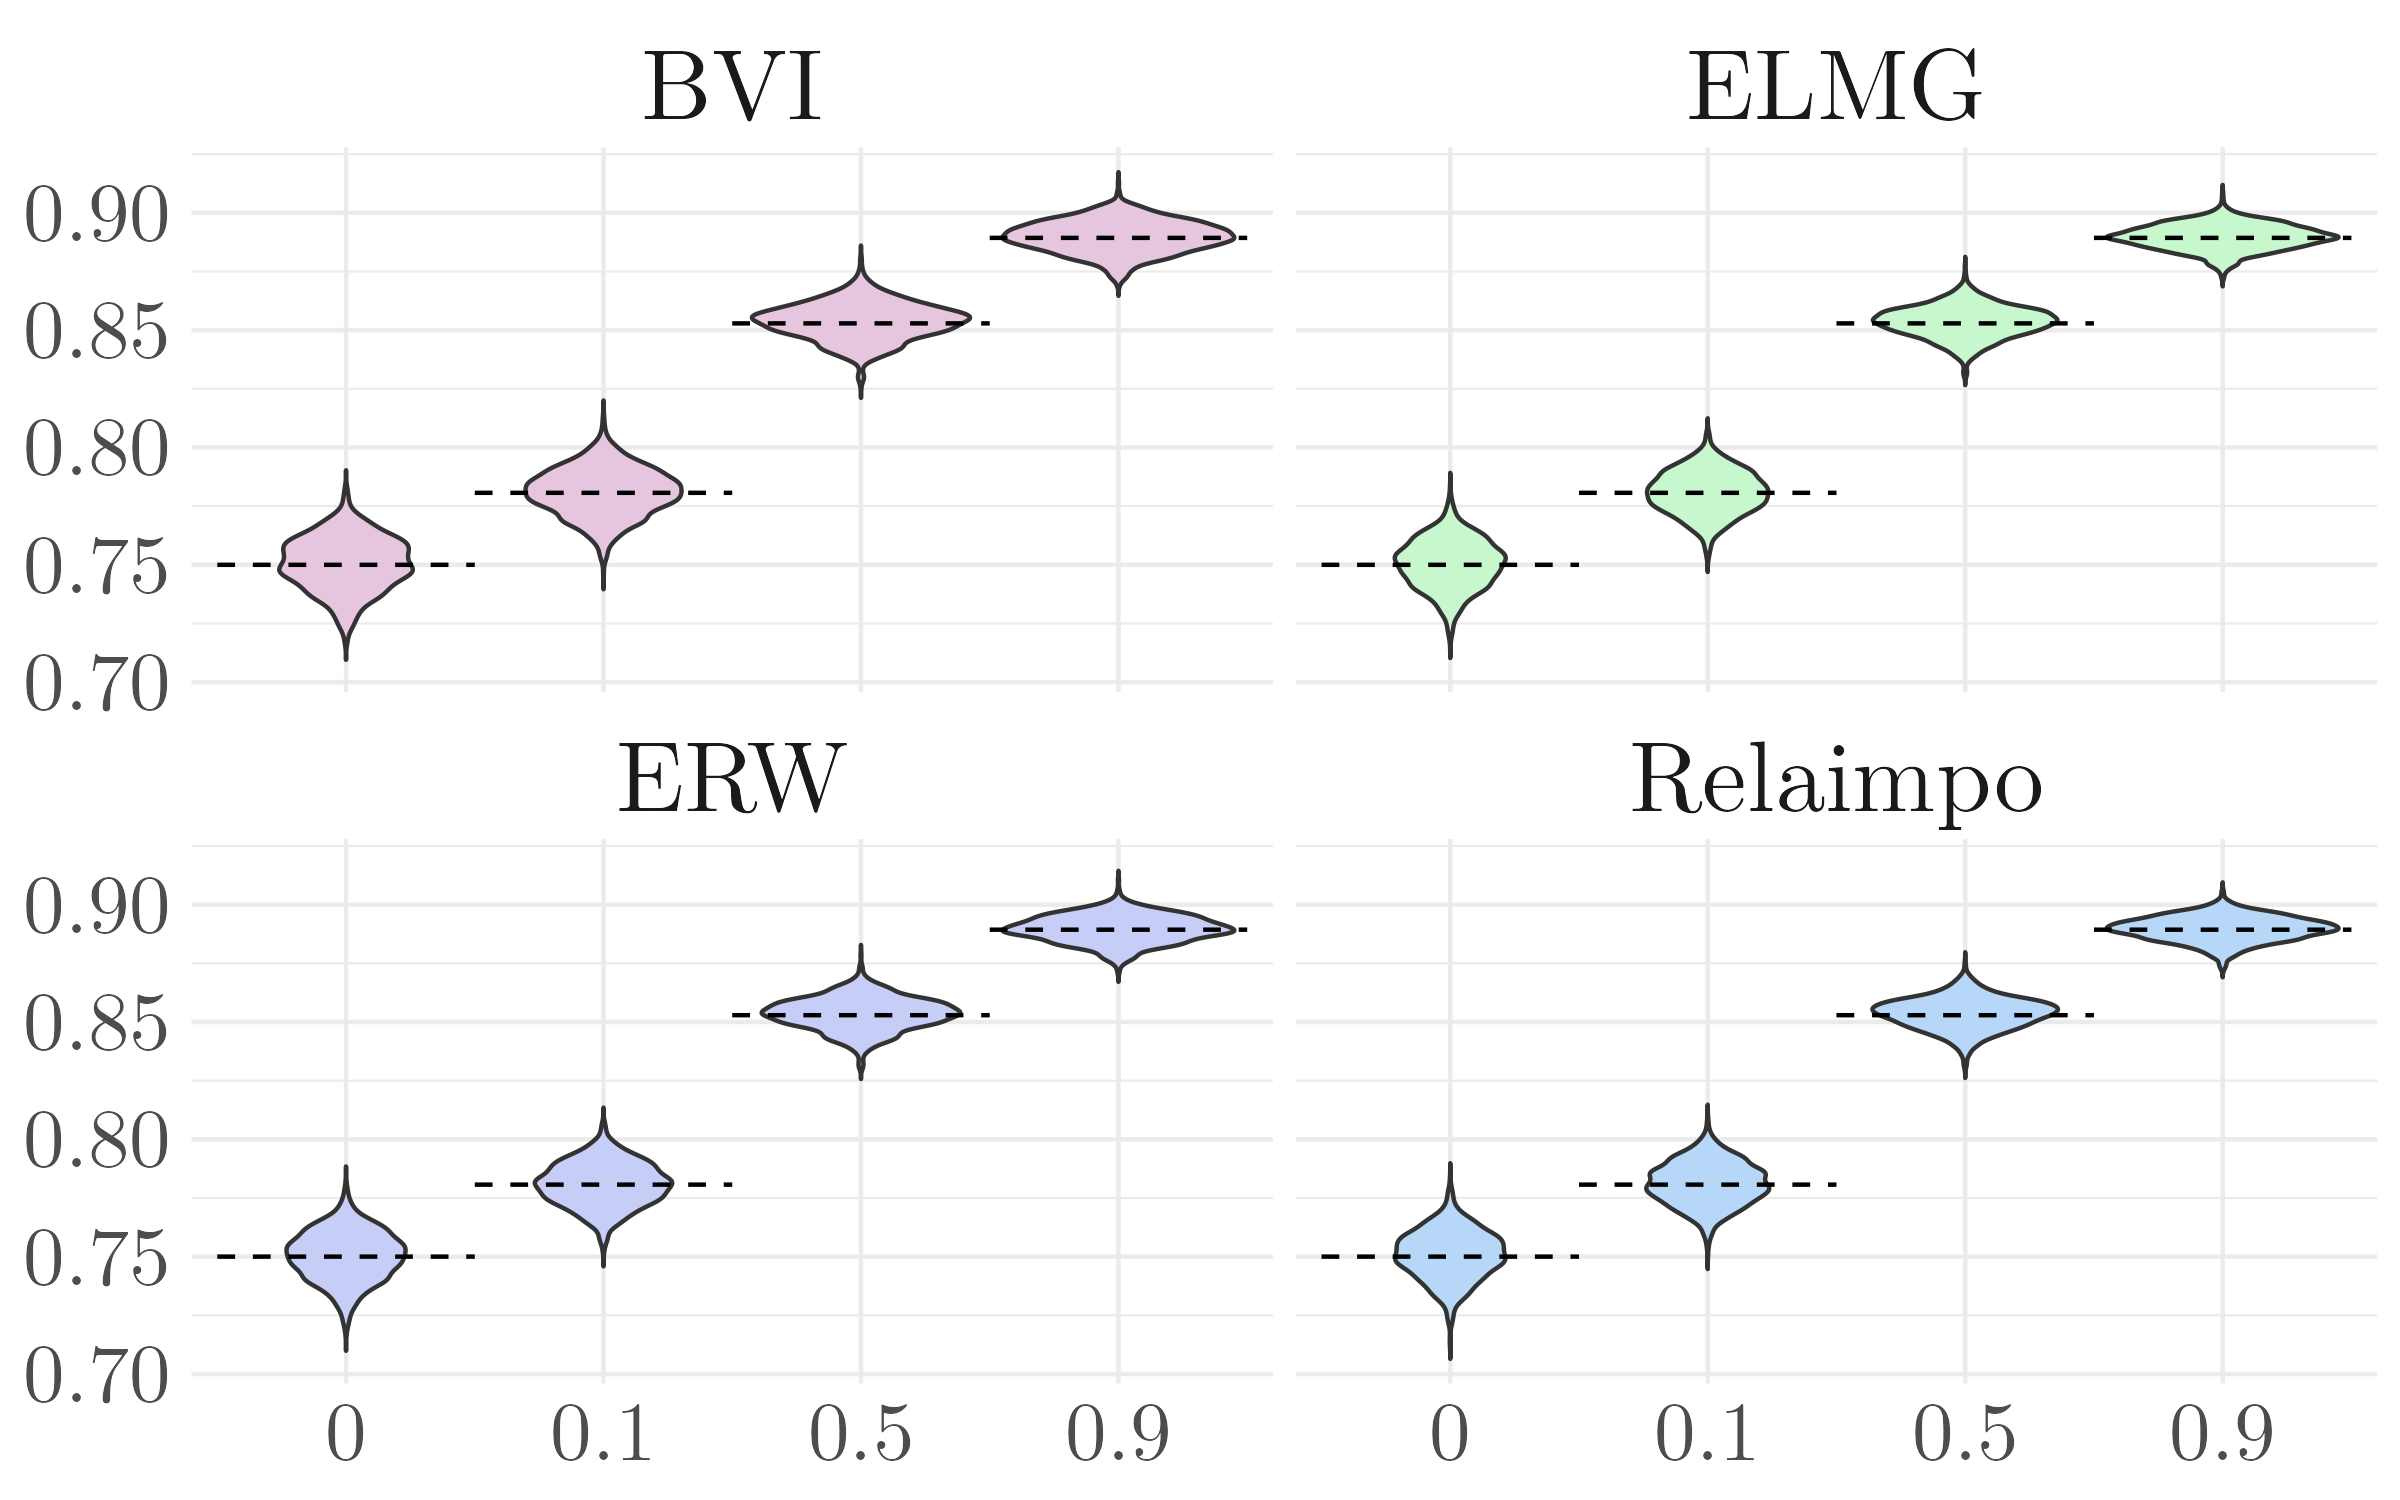
\includegraphics[width=0.55\linewidth]{Figures/ViolinPlots/Marginal_Variance.png}
    \label{fig:variance_marginal}
  }
  \hfill
  \subfloat{
    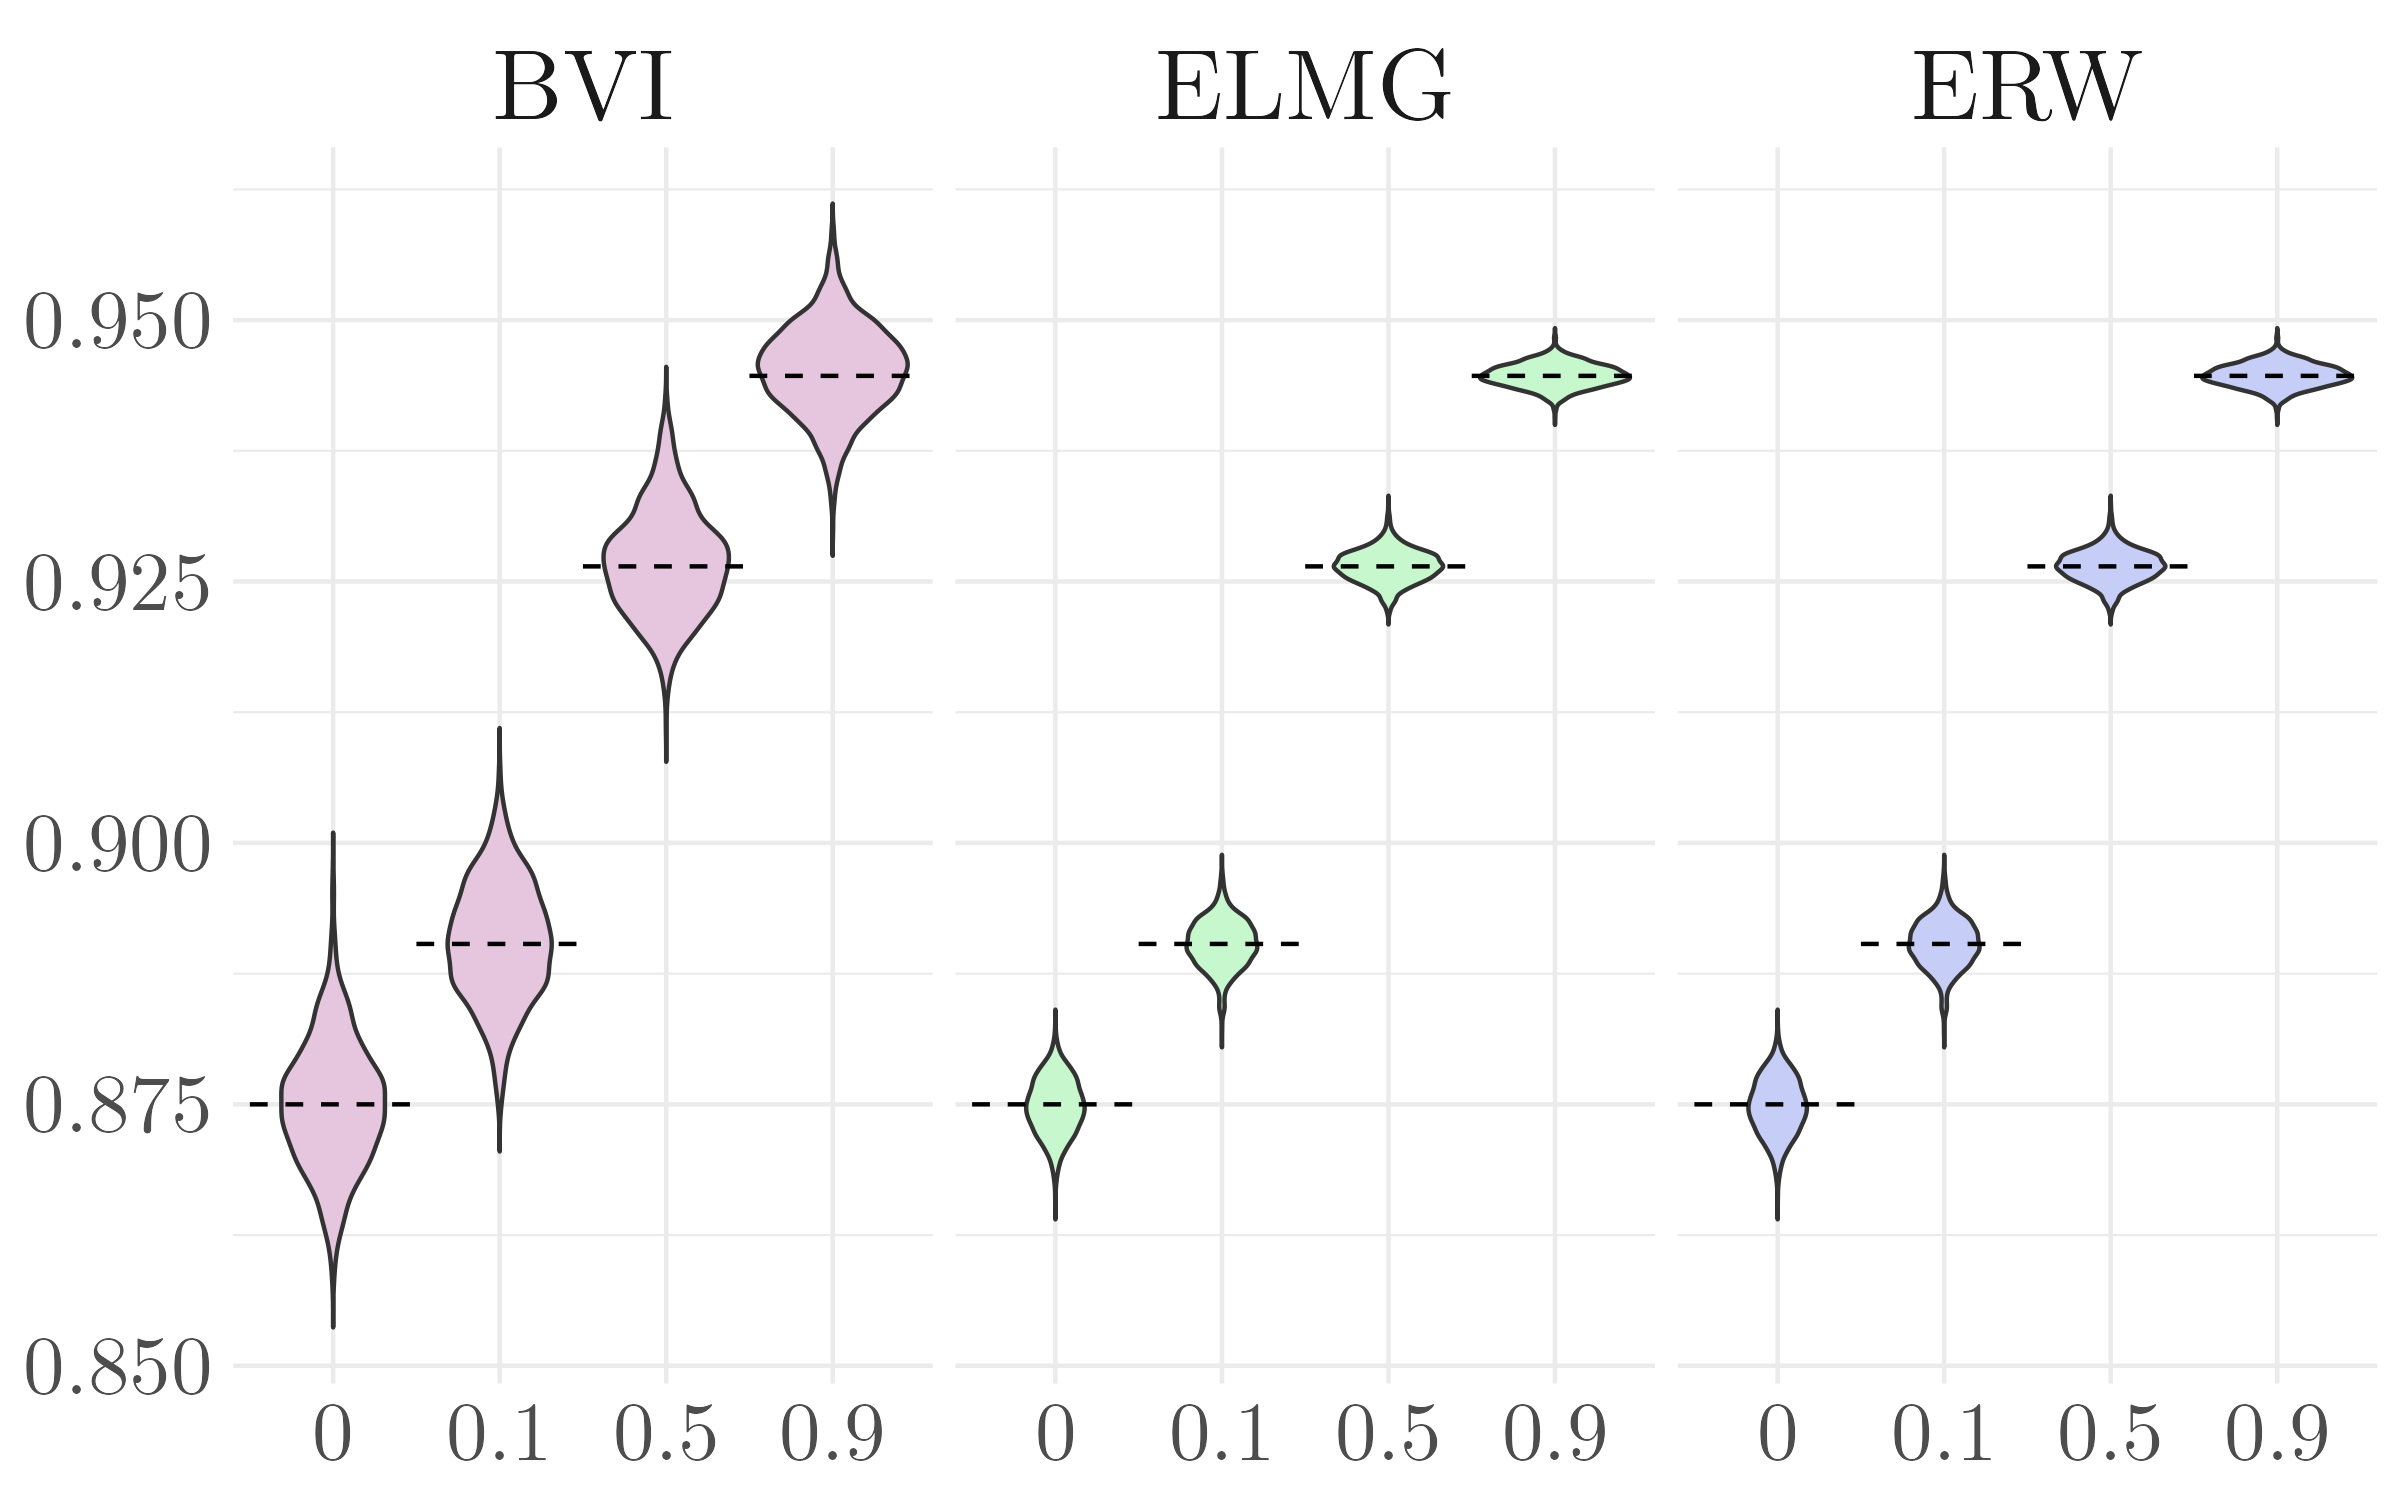
\includegraphics[width=0.55\linewidth]{Figures/ViolinPlots/Conditional_Variance.png}
    \label{fig:variance_conditional}
  }
  \caption[Marginal and conditional $R^2$ in Gaussian LMM]{Violin plots for the total marginal (top) and conditional (bottom) variance explained ($R^2$) for different correlation levels displayed along the x-axis, calculated from the ensemble of $N_{\text{sim}}=10^4$ simulated datasets by the BVI, ELMG, the ERW and the Relaimpo method(only marginal variance explained can be computed). For the BVI method the posterior means of the sampled posterior distributions of $\boldsymbol{\beta}$ and the marginal distribution of $\hat{\sigma}^2_{\alpha}$ in each simulation are used to compare to the point estimates of the other two methods. The horizontal lines display the theoretical explained variance for each correlation level $\rho$ as in \Cref{table:2}.}
  \label{fig:total_variance}
\end{figure}

\section{Modelling house sparrow traits}
\label{sec:heritability_results}
We now investigate the results of applying our method to the house sparrow dataset. The presented results contain the sampled relative importance distributions of the covariates used to model body mass, wing length and tarsus length. By including the full analysis, we want to demonstrate that our method enables a comprehensive analysis by providing the relative variable importance of all covariates. A particular analysis is done on the heritability, as this is a special case of relative importance (\Cref{sec:heritability}) and is the focus of much research. The samples of heritability are sampled from the variance component that captures additive genetic variance (\textit{IDC2}), and we use the results from \citet{Silva2017} and \citet{Muff2019Genetic} for comparison. More detailed plots of the estimated posterior heritability distributions are available in \Cref{sec:supplementary_sparrows}. For the house sparrow analysis, the covariance structure of the pedigree required us to model more complex random effects than i.i.d. random intercepts, and so the \texttt{rptR} package could not be used for comparisons. In \Cref{table:summary_heritability} the mean of sampled heritability along with quantile values is presented, as well as the corresponding measures from the comparable studies.
% \begin{table}[H]
%   \centering
%   \begin{tabular}{lccccccc}
%   \toprule
%    & \multicolumn{2}{c}{\citet{Silva2017}} & \multicolumn{2}{c}{\citet{Muff2019Genetic}} & \multicolumn{2}{c}{BVI} \\ 
%    \cmidrule(lr){2-3} \cmidrule(lr){4-5} \cmidrule(lr){6-7}
%    & Estimate & CI & Estimate & CI & Mean & CI \\ 
%   \midrule
%   $h^2_{\text{mass}}$    & 0.300 & [0.231, 0.369] & 0.288 & [0.219, 0.371] & 0.283 & [0.232, 0.344] \\
%   $h^2_{\text{wing}}$    & 0.388 & [0.353, 0.461] & 0.344 & [0.294, 0.409] & 0.356 & [0.322, 0.393] \\
%   $h^2_{\text{tarsus}}$  & 0.415 & [0.333, 0.497] & - & - & 0.401 & [0.330, 0.470] \\ 
%   \bottomrule
%   \end{tabular}
%   \caption[Heritability estimates and confidence intervals]{Heritability estimates and confidence interval from \citet{Silva2017}, posterior means of additive genetic variance divided by the posterior means of total phenotypic variance in \citet{Muff2019Genetic} with corresponding confidence interval and the mean and confidence interval of the heritability samples obtained from the BVI method for the phenotypic traits; body mass, wing length and tarsus length.}
%   \label{table:summary_heritability}
% \end{table}
\begin{table}[H]
  \centering
  \small
  \begin{tabular}{lccccccc}
    \toprule
    & \multicolumn{2}{c}{$h^2_{\text{mass}}$} & \multicolumn{2}{c}{$h^2_{\text{wing}}$} & \multicolumn{2}{c}{$h^2_{\text{tarsus}}$} \\
    \cmidrule(lr){2-3} \cmidrule(lr){4-5} \cmidrule(lr){6-7}
    & Est. & CI & Est. & CI & Est. & CI \\
    \midrule
    \citet{Silva2017} & 0.300 & [0.231, 0.369] & 0.388 & [0.353, 0.461] & 0.415 & [0.333, 0.497] \\
    \citet{Muff2019Genetic} & 0.288 & [0.219, 0.371] & 0.344 & [0.294, 0.409] & - & - \\
    %BVI grid & 0.282 & [0.231, 0.342] & 0.356 & [0.322, 0.393] & 0.401 & [0.329, 0.468] \\
    BVI & 0.284 & [0.255, 0.315] & 0.356 & [0.334, 0.380] & 0.401 & [0.363, 0.438] \\
    \bottomrule
  \end{tabular}
  \caption[Heritability estimates and confidence intervals]{Heritability estimates and confidence intervals from \citet{Silva2017}, posterior means of additive genetic variance divided by the posterior means of total phenotypic variance in \citet{Muff2019Genetic} with corresponding confidence intervals, and the mean and quantile values of the heritability samples obtained from the BVI method, for the phenotypic traits: body mass, wing length, and tarsus length. Note that in \citet{Muff2019Genetic} no estimate of tarsus length heritability was provided.}
  \label{table:summary_heritability}
\end{table}
\noindent For the sampled heritability of body mass, we have a mean of $0.284$ and the interval $[0.255, 0.315]$ covers the $95$th percentile (\Cref{table:summary_heritability}). In general, the posterior distribution of heritability has a Gaussian shape, centered around the mean value (\Cref{fig:heritability_mass_combined}). The posterior distribution of relative importance of the fixed effects predominantly shows very small values. Recall that importance calculations of fixed effects include squaring the coefficients, and so no negative importance can be allocated to a covariate. Notably, the relative importance of covariates \textit{FGRM} and \textit{other} exhibits a negative exponential decay pattern, while the covariates \textit{sex, age} and \textit{outer} seem to have a skewed normal distribution. The posterior distribution of relative importance allocated to \textit{month} looks normally distributed. Considering the random effects, it is evident that they have been allocated a much larger share of importance compared to the fixed effects. The importance of the Gaussian observations have a normal shape and are often allocated over $50\%$ of the total importance. The distribution of importance for \textit{IDC}, which is the covariate accounting for individual differences, does not seem to follow any standard distribution. Lastly, \textit{hatchyear} is allocated a quite small importance, and the distribution looks like a skewed normal distribution. To fit the model and obtain the samples, the BVI method took about $73$ seconds. Overall, the heritability values for body mass are in close agreement with the estimates from \citet{Silva2017} and \citet{Muff2019Genetic}, and the posterior importance distributions for all covariates seem to be reasonable. 
\begin{figure}[H]
  \centering
  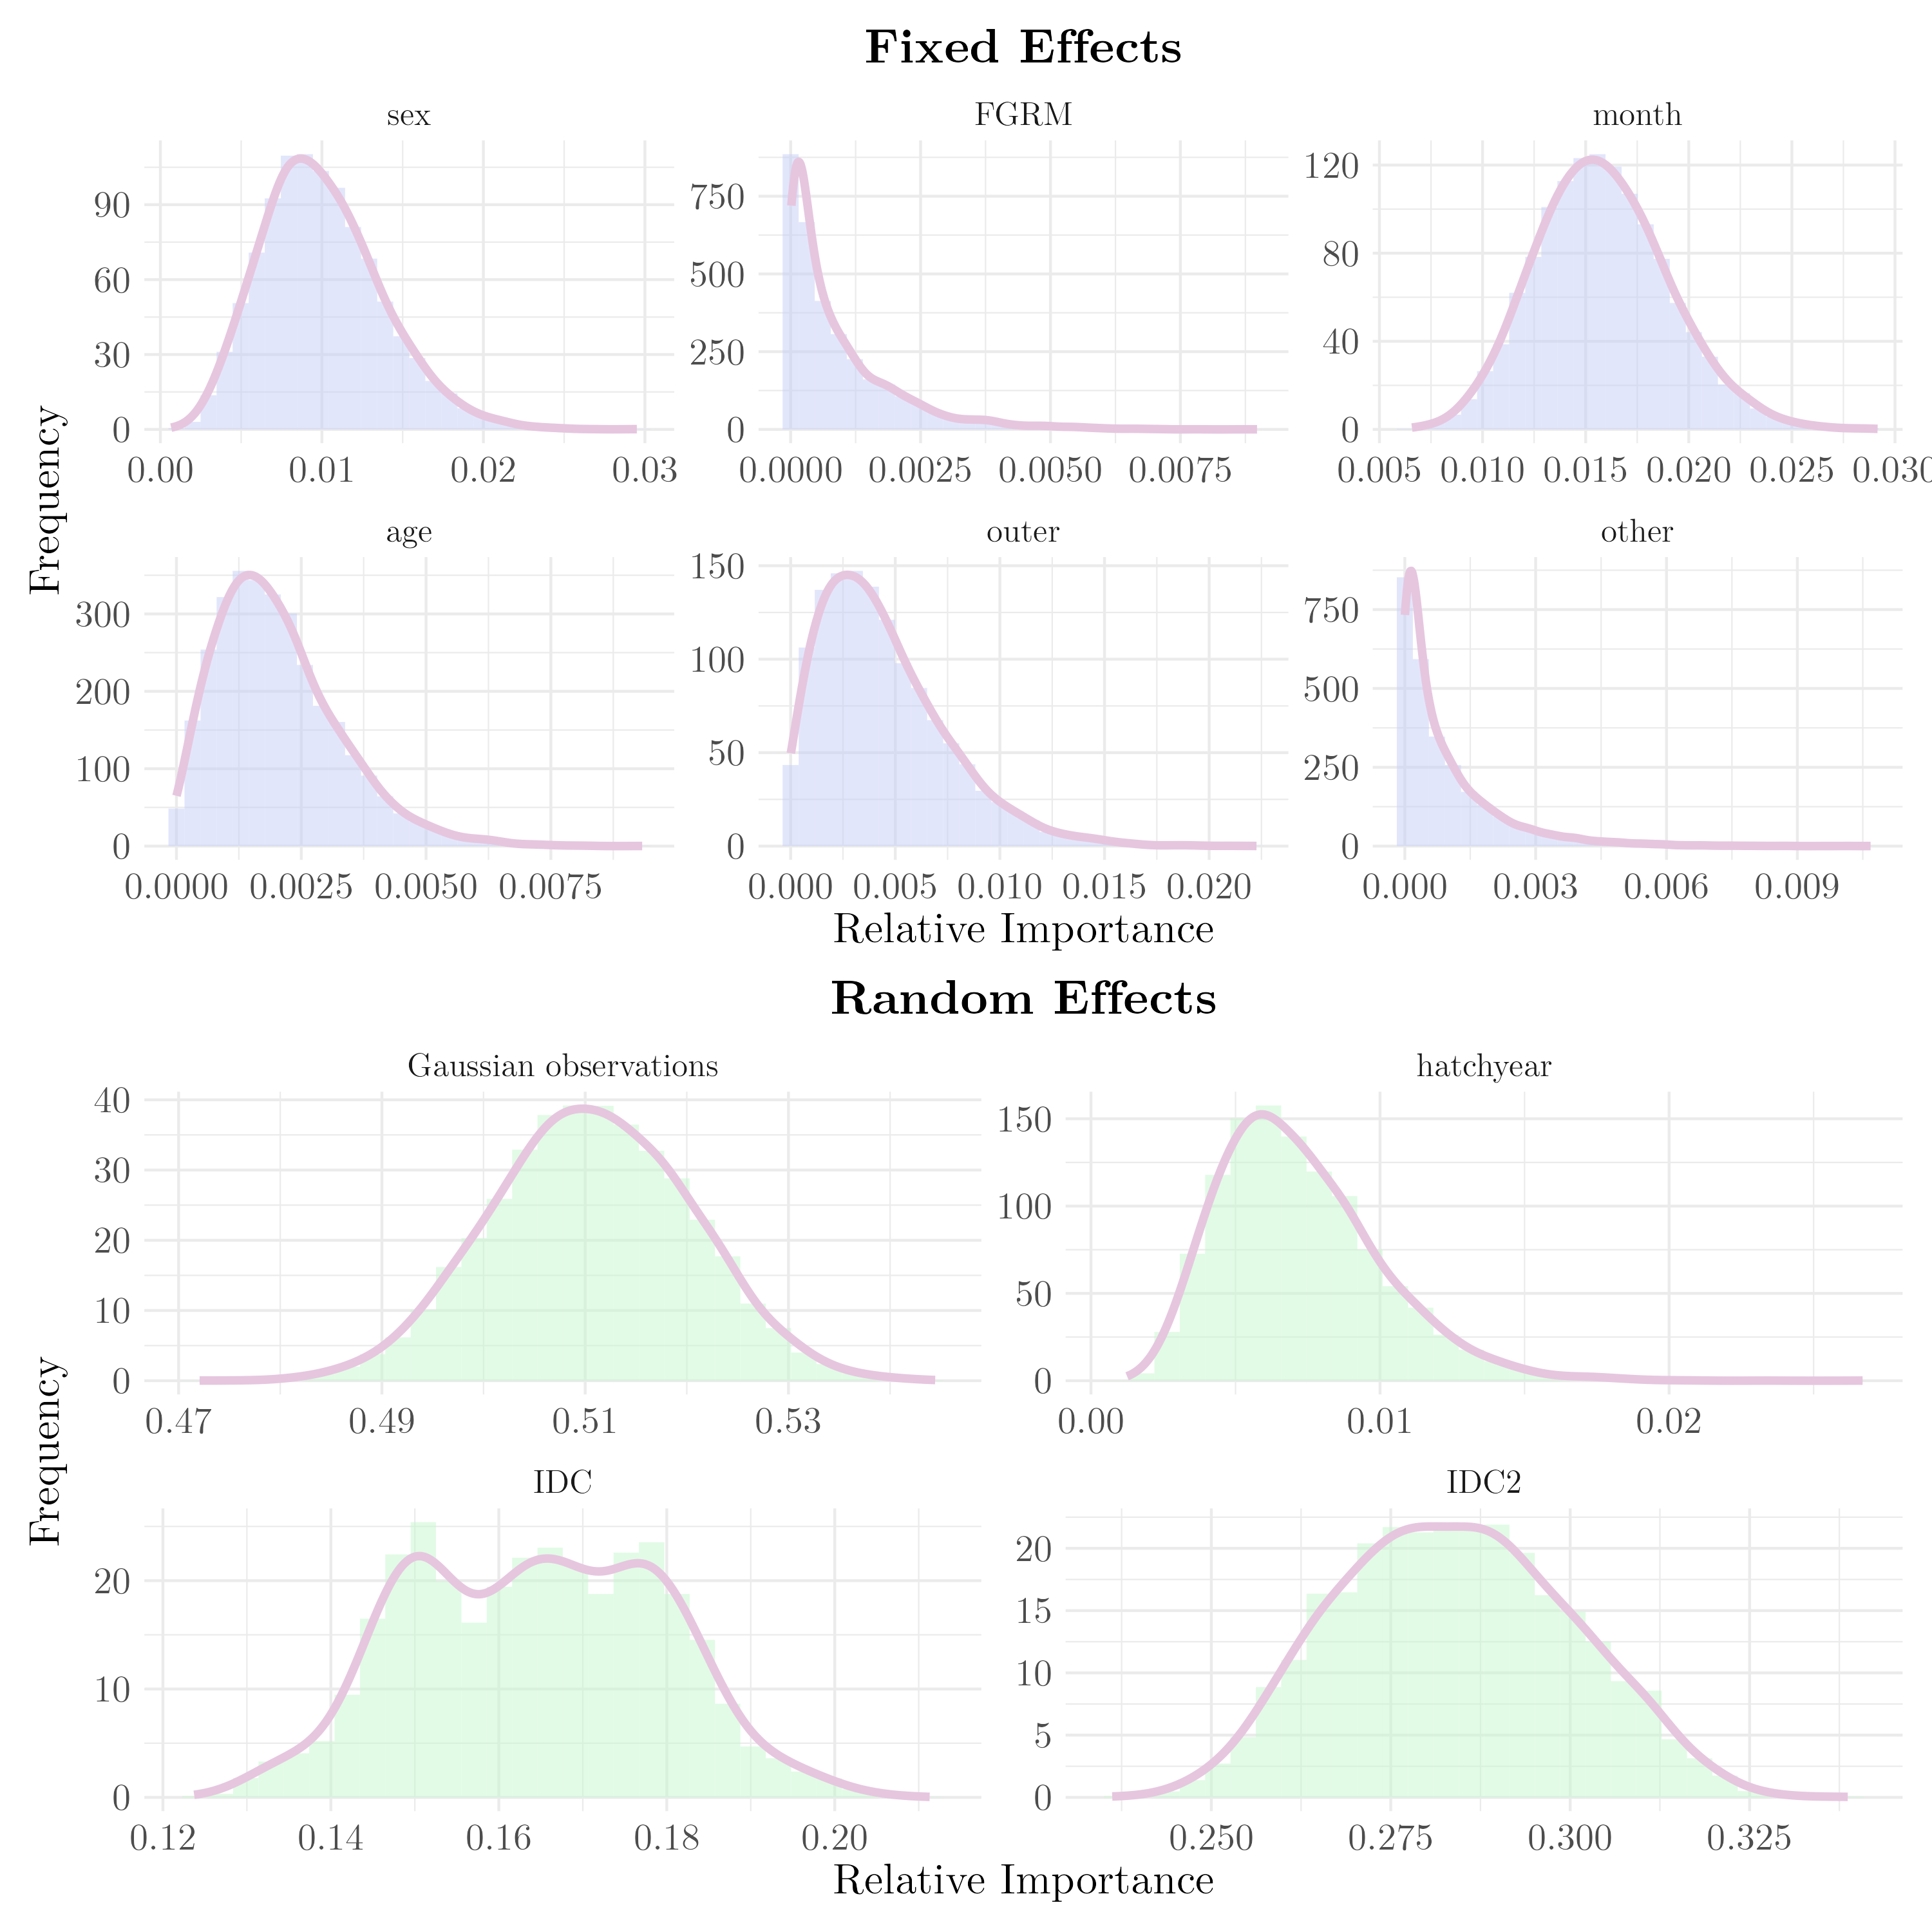
\includegraphics[width=1\linewidth]{Figures/House sparrow study/Mass_ccd.png}
  \caption[Estimated posterior importance of all covariates in the body mass model from the BVI method]{Histogram depicting the sampled posterior importance values of all covariates used to model body mass by the BVI method for the house sparrow dataset. The heritability estimates correspond to the random effect \textit{IDC2}, and the estimates from the BVI method, \citet{Silva2017} and \citet{Muff2019Genetic} of heritability are found in \Cref{table:summary_heritability}.}
  \label{fig:heritability_mass_combined}
\end{figure}
% \begin{figure}[H]
%   \centering
%   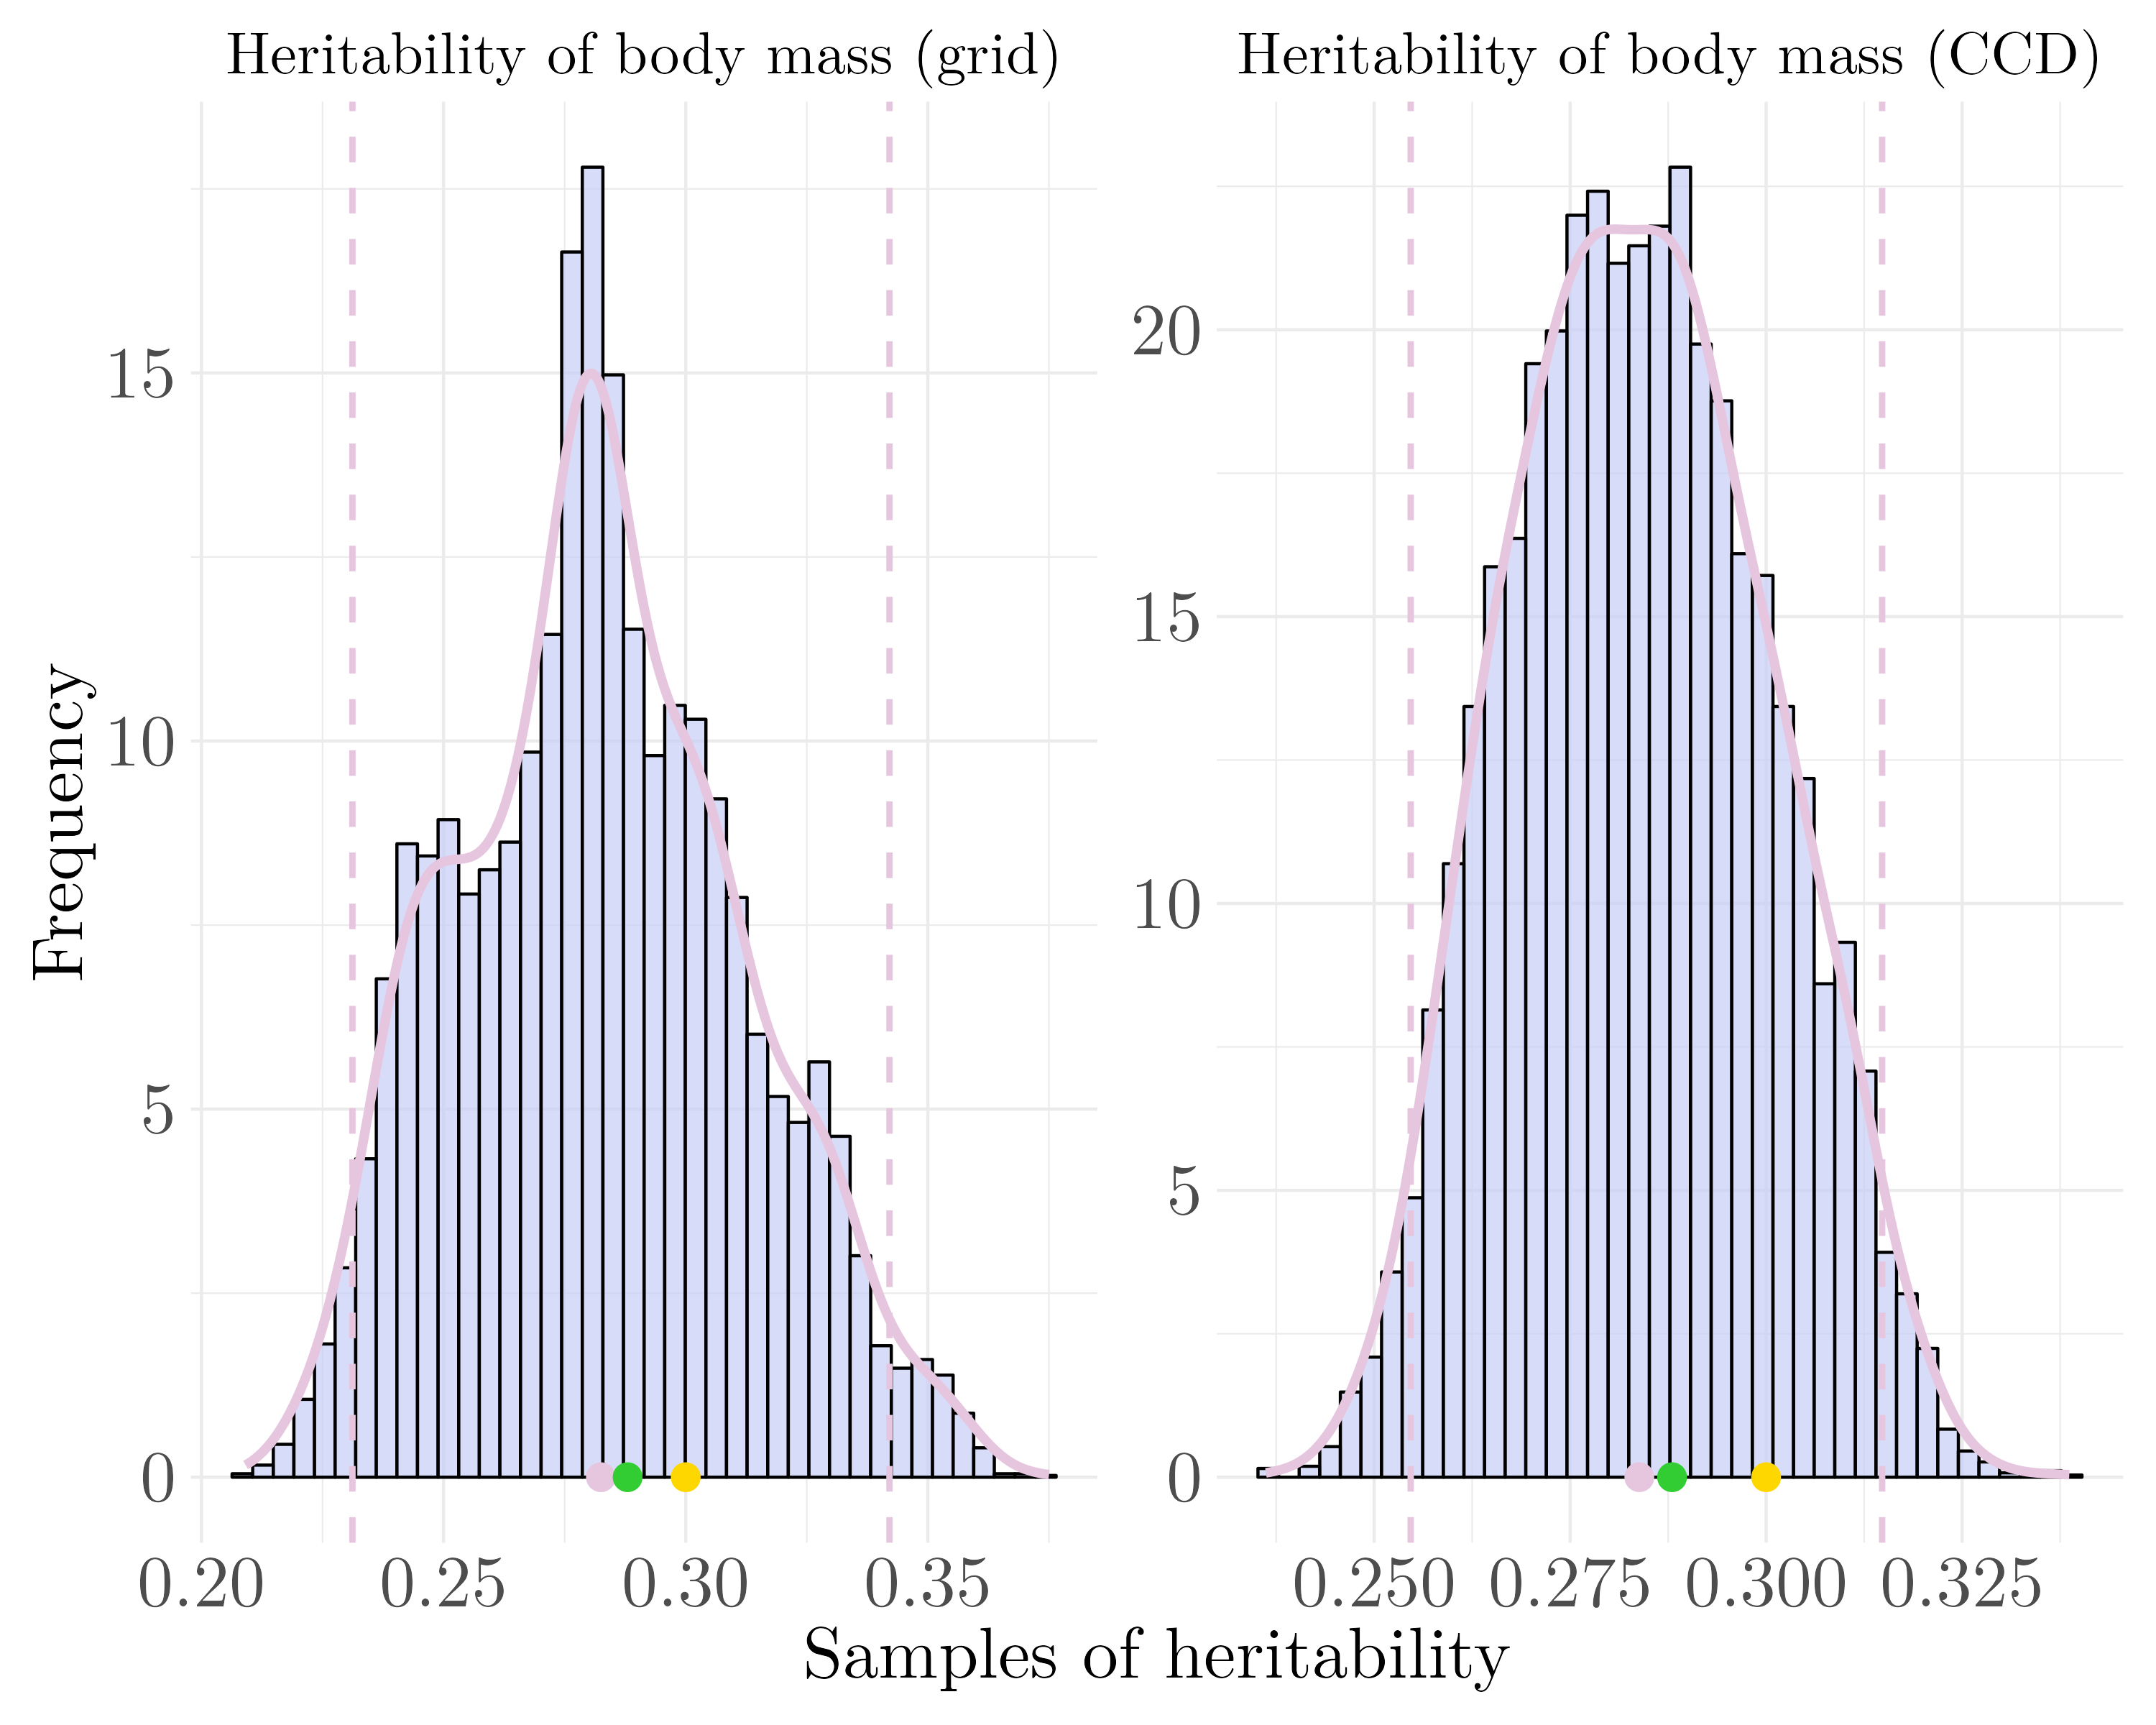
\includegraphics[width=1\linewidth]{Figures/House sparrow study/Heritability_mass_combined.png}
%   \caption[Estimated heritability of body mass from grid and CCD strategy]{Histogram depicting the estimated heritability values of body mass by the BVI method for the grid integration strategy(left) and CCD integration strategy (right) for the house sparrow dataset. The mean of the samples is marked as a pink circle at the bottom of the histogram, with the lower and upper value for the $95\%$ percentile marked as dashed lines. The heritability estimate from \citet{Silva2017} and \citet{Muff2019Genetic} are marked as gold and green dots respectively at the bottom of the histogram.}
%   \label{fig:heritability_mass_combined}
% \end{figure}
\noindent The samples of wing length heritability form a symmetric bell curve, around the mean of $0.356$ (\Cref{fig:heritability_wing_combined} and \Cref{table:summary_heritability}). Further, the $95$th percentile is roughly the interval $[0.334, 0.380]$, which is more narrow than the quantile for the heritability of body mass. Contrary to what was the case for body mass, when modelling wing length, some fixed effects are allocated a significant share of importance. For instance, the distribution of relative importance for \textit{sex} and \textit{age} are centered around $0.340$ and $0.055$ respectively, while the others are allocated an importance of the same order of magnitude as for body mass. Again, some fixed covariates exhibit a decay pattern close to zero (\textit{e.g. FGRM} and \textit{age}), and some seem to have a skewed normal shape (\textit{e.g. sex} and \textit{outer}). For the random effects, we notice that the Gaussian observations are normally distributed and allocated roughly $17.5\%$ of the total importance. Again the \textit{hatchyear} effect is allocated a small importance, and the posterior importance distribution for \textit{IDC} is not easily interpretable, but contains smaller estimates than for body mass. For wing length, the BVI method took about $76$ seconds to fit the model and draw the samples. The heritability estimate from the BVI method lies between the estimates of \citet{Silva2017} and \citet{Muff2019Genetic}, and again we find the posterior importance distributions for all covariates to be plausible.
\begin{figure}[H]
  \centering
  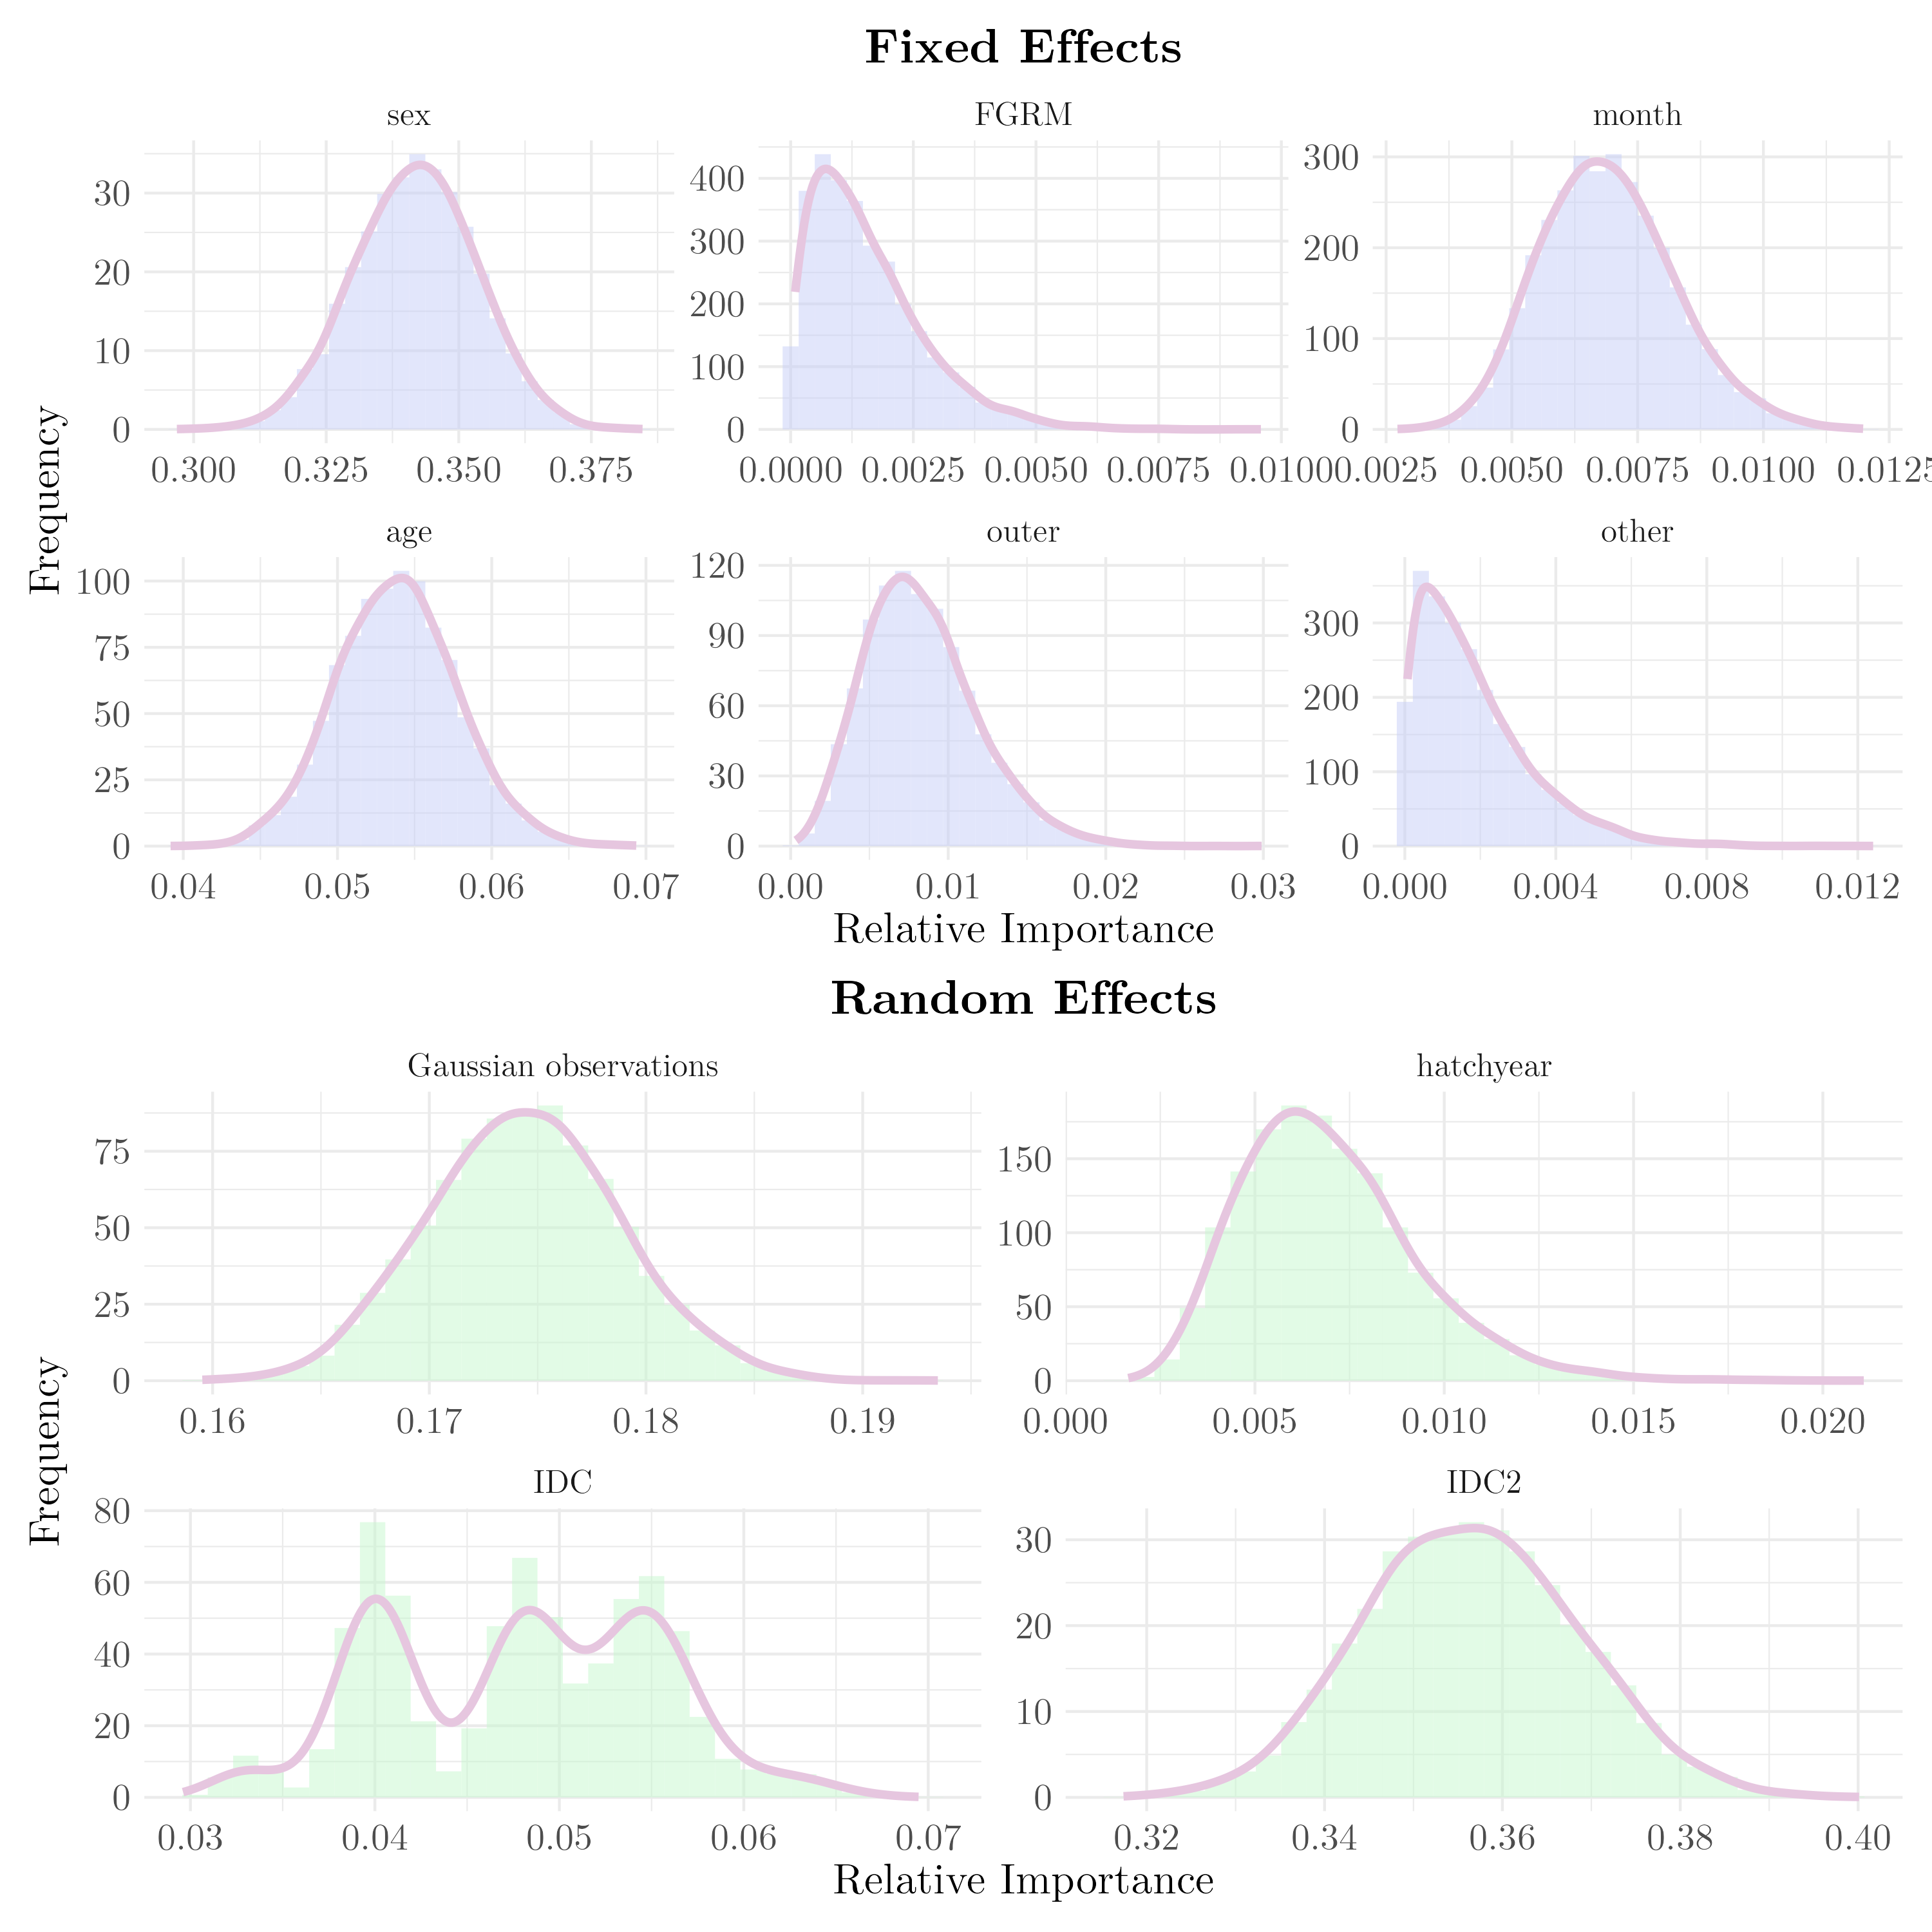
\includegraphics[width=1\linewidth]{Figures/House sparrow study/Wing_ccd.png}
  \caption[Estimated posterior importance of all covariates in the wing length model from the BVI method]{Histogram of the sampled posterior importance values for the covariates modelling wing length from the house sparrows, estimated by the BVI method. The heritability estimates correspond to the random effect \textit{IDC2}, and the estimates from the BVI method, \citet{Silva2017} and \citet{Muff2019Genetic} of heritability are found in \Cref{table:summary_heritability}.}
  \label{fig:heritability_wing_combined}
\end{figure}
% \begin{figure}[H]
%   \centering
%   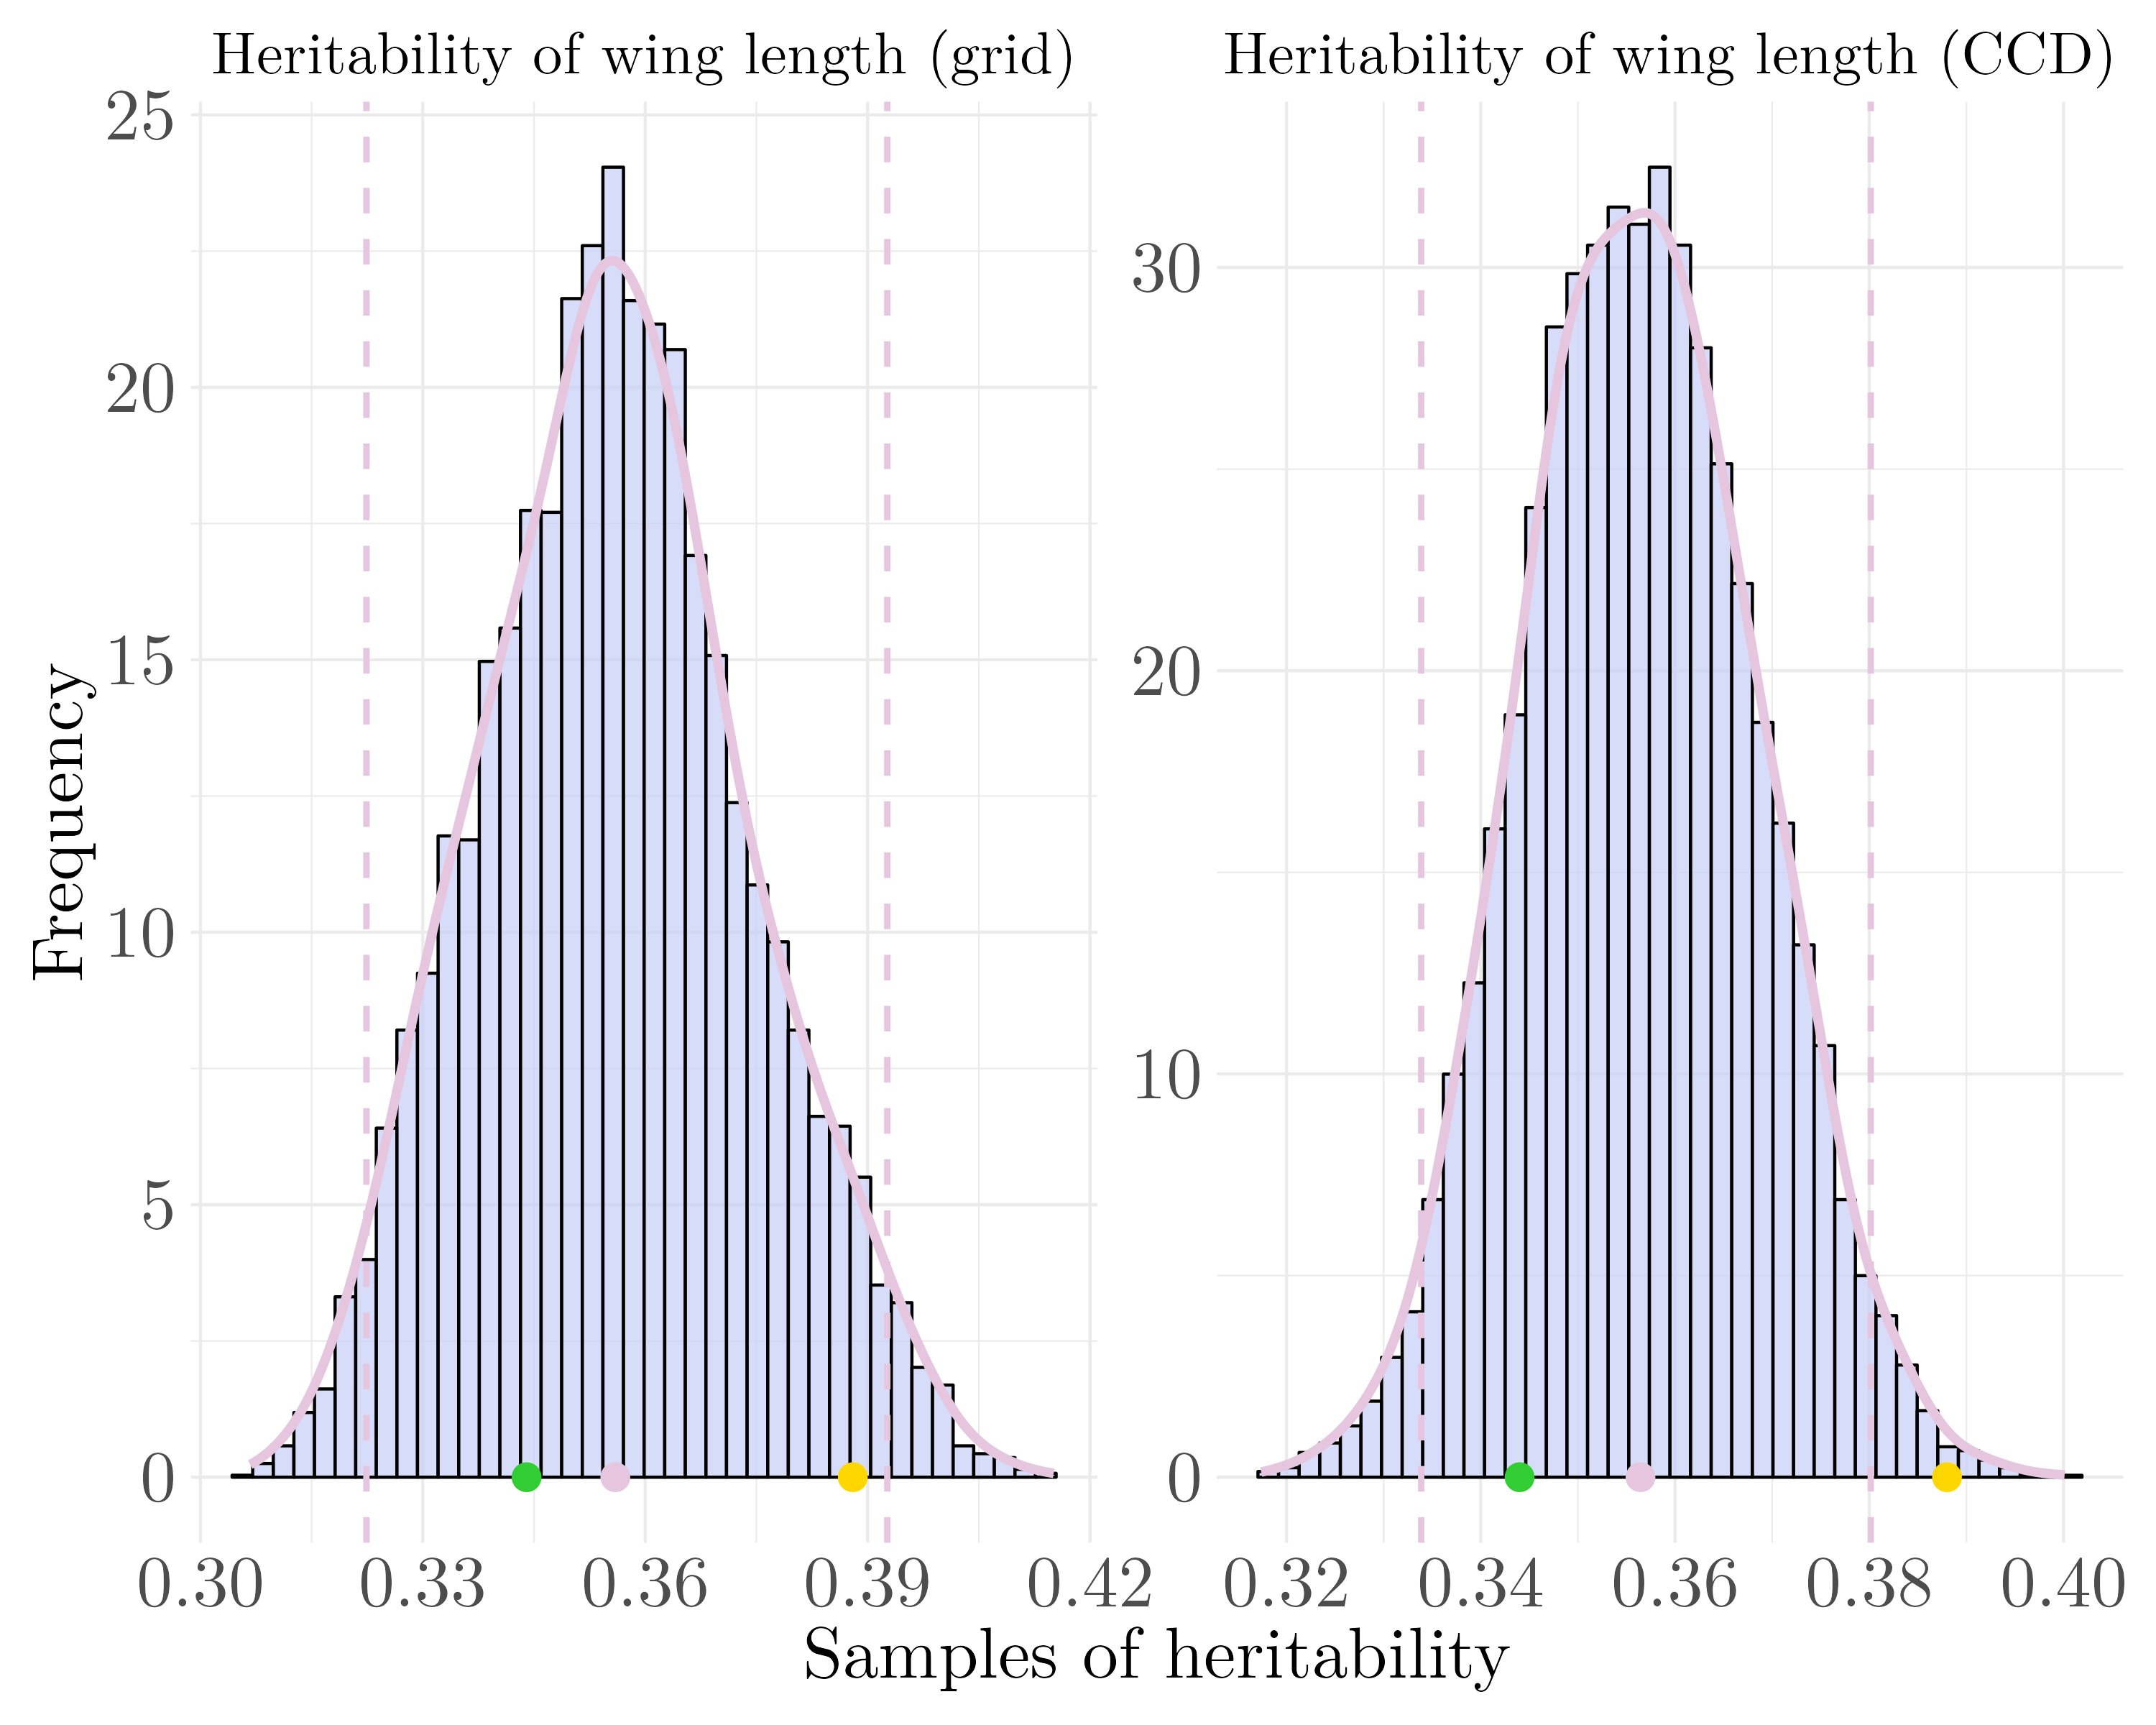
\includegraphics[width=1\linewidth]{Figures/House sparrow study/Heritability_wing_combined.png}
%   \caption[Estimated heritability of wing length]{Histogram of heritability values for wing length of the house sparrows estimated by the BVI method for the grid integration strategy (left) and the CCD integration strategy (right). The mean of the samples is marked as a pink circle at the bottom of the histogram, and the lower and upper value for the $95\%$ percentile are featured as dashed lines. The heritability estimate from \citet{Silva2017} and \citet{Muff2019Genetic} are marked as gold and green dots respectively at the bottom of the histogram.}
%   \label{fig:heritability_wing_combined}
% \end{figure}
\noindent The heritability samples of tarsus length has a mean of $0.401$ and the estimated $95$th quantile is $[0.363, 0.438]$ (\Cref{table:summary_heritability}). This is the largest quantile for all traits, and the posterior distribution of tarsus length heritability seems normal with a broader and flatter peak than for body mass and wing length (\Cref{fig:heritability_tarsus_combined}). As for the body mass model, the posterior distribution of the relative importance allocated to the fixed covariates used to model tarsus length mainly consist of very low values. Here, a strong decay pattern is observable for \textit{age, outer} and \textit{other}, and a moderate decay for \textit{sex} and \textit{FGRM}. The only fixed covariate that looks to have a normal shape is \textit{month}. Conspicuously, the Gaussian observations are given a small share of importance, with a bell curve centered between $0.031$ and $0.032$. The importance of the random effect \textit{hatchyear} is also for tarsus length very small, and the distribution of importance allocated to \textit{IDC} is now a bell curve with a relatively large mean of around $0.538$. To model tarsus length and draw samples, the BVI reported a runtime of $74$ seconds. No heritability estimate from \citet{Muff2019Genetic} was available, however the estimate from the BVI method is close to that of \citet{Silva2017}. 
The posterior importance distributions for all covariates seem reasonable, but the small importances allocated to the random error (Gaussian observations) should be met with caution. 
\begin{figure}[H]
  \centering
  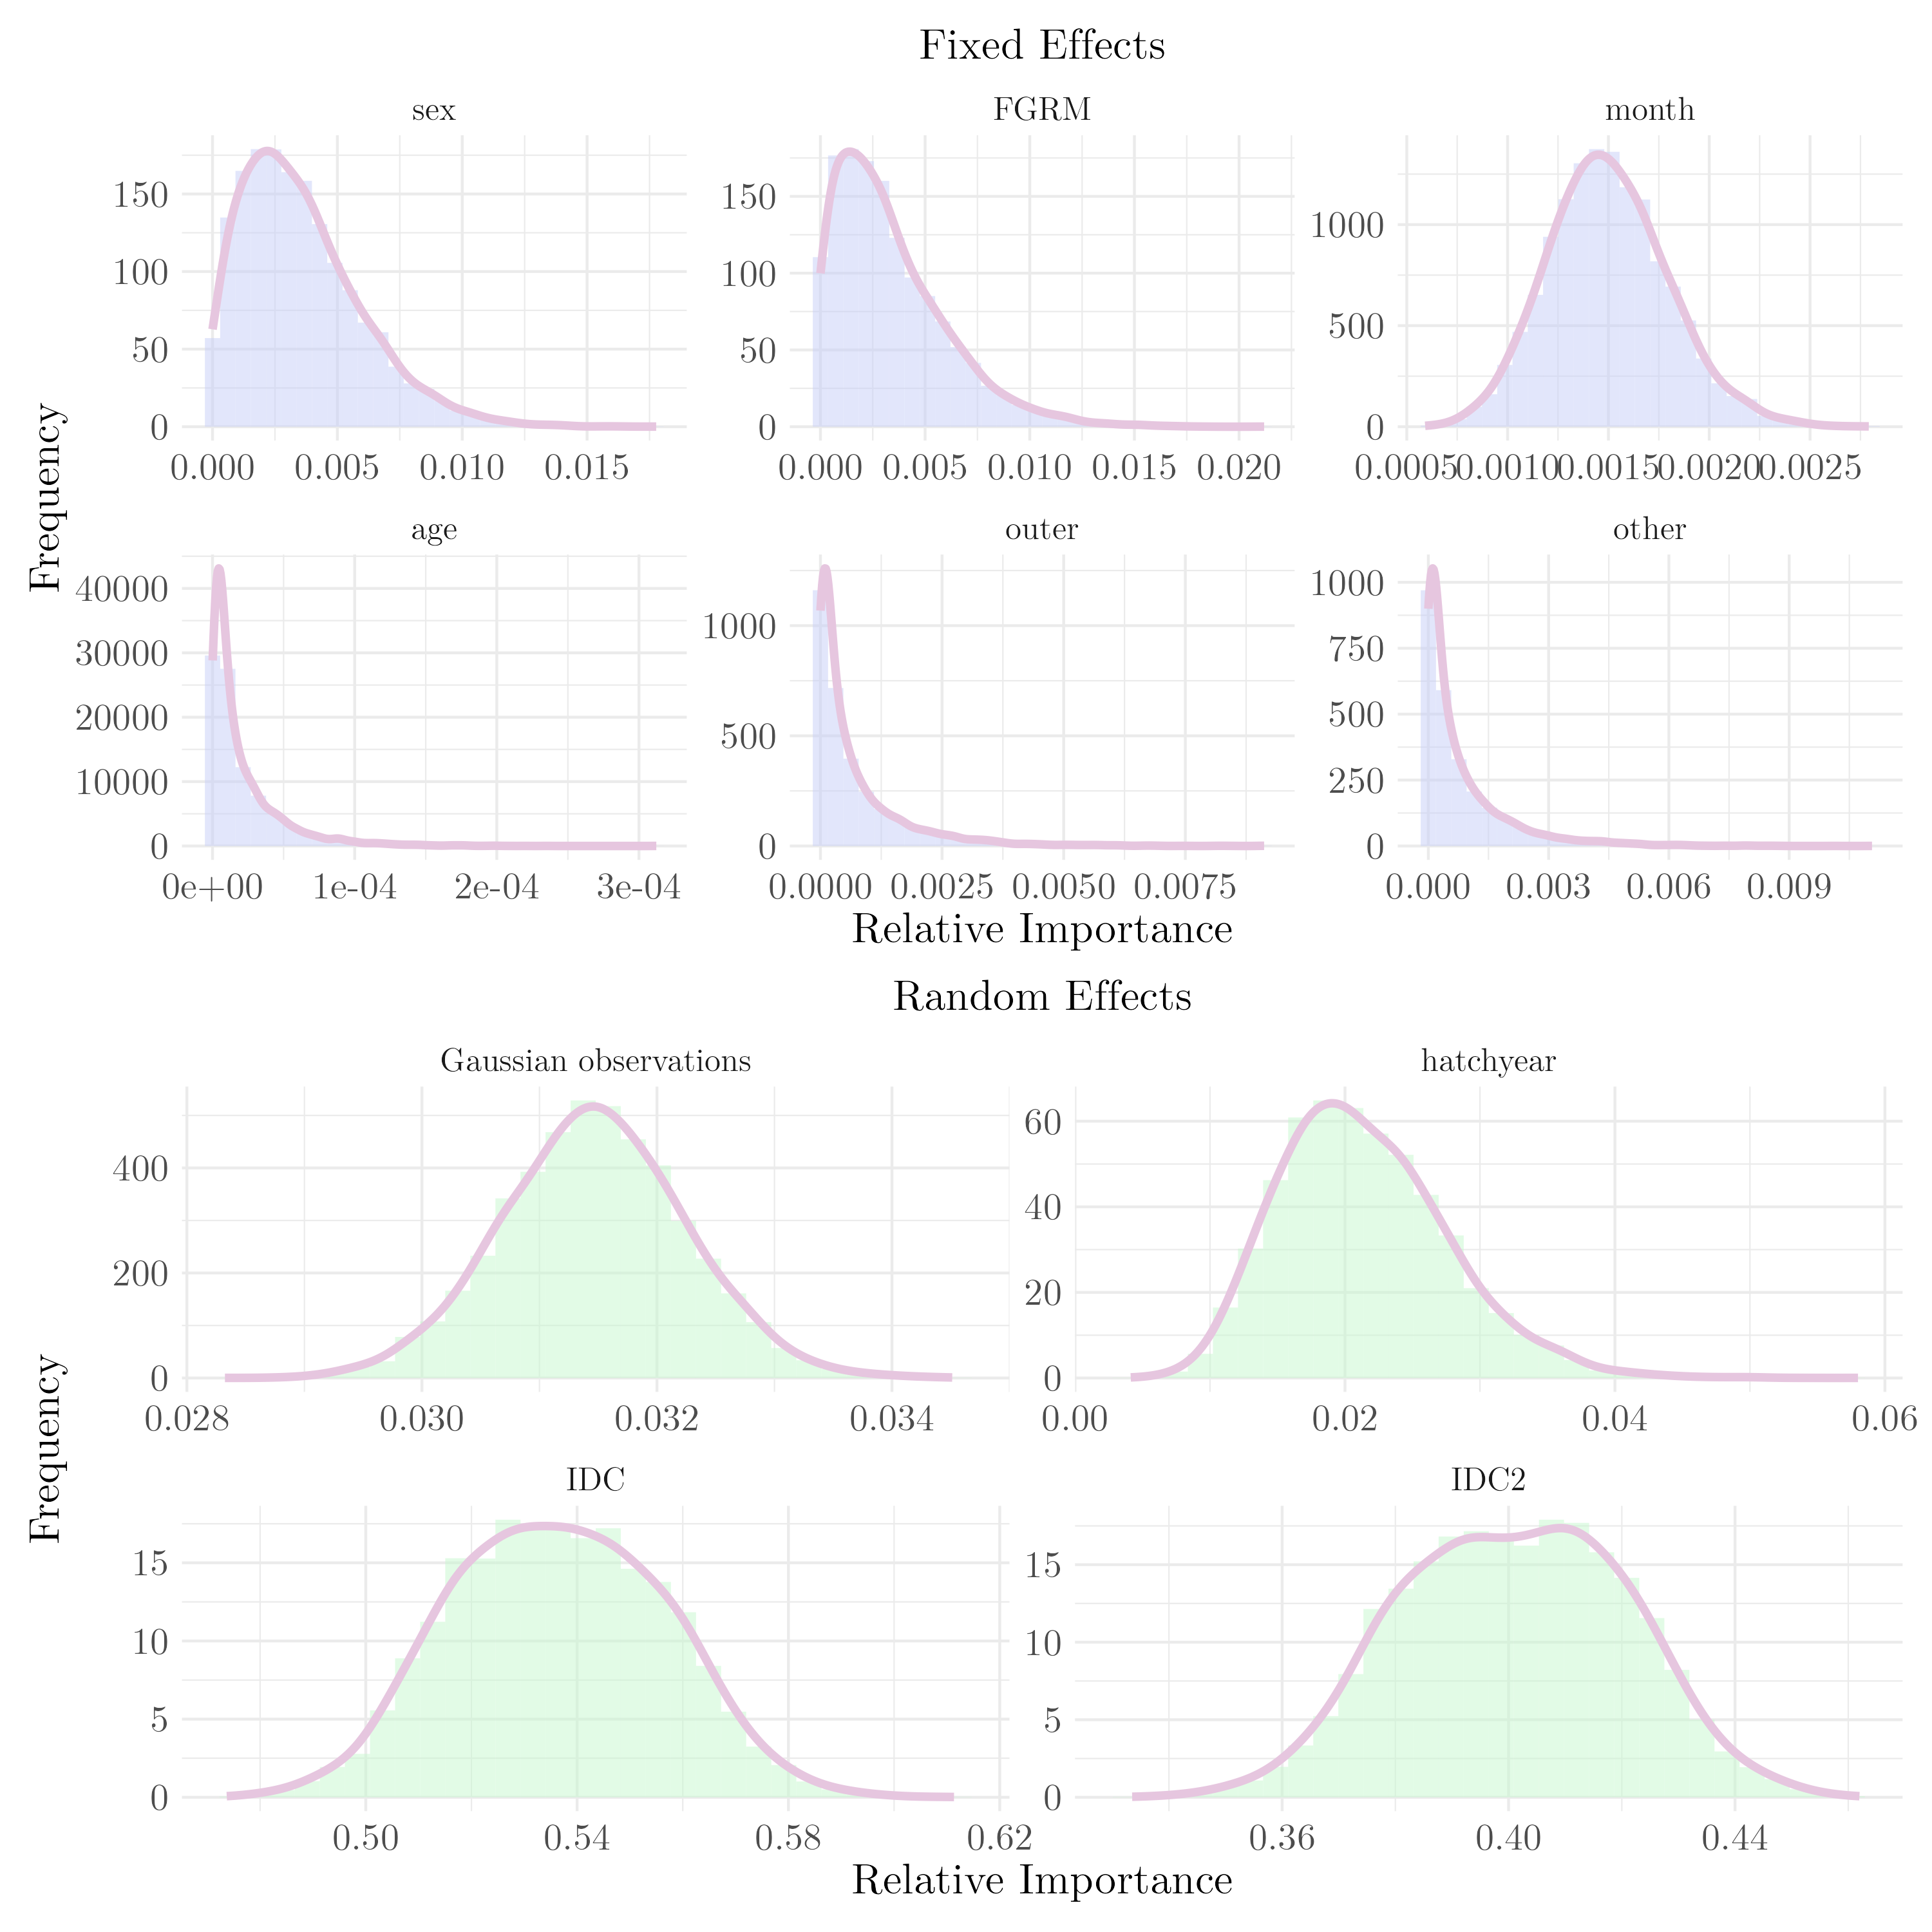
\includegraphics[width=1\linewidth]{Figures/House sparrow study/Tarsus_ccd.png}
  \caption[Estimated posterior importance of all covariates in the tarsus length model from the BVI method]{Histogram of the sampled posterior importance values for covariates used in the tarsus length model of the house sparrows, estimated by the BVI method. The heritability estimates correspond to the random effect \textit{IDC2}, and the estimates from the BVI method and \citet{Silva2017} of heritability are found in \Cref{table:summary_heritability}. No estimate from \citet{Muff2019Genetic} was available.}
  \label{fig:heritability_tarsus_combined}
\end{figure}
% \begin{figure}[H]
%   \centering
%   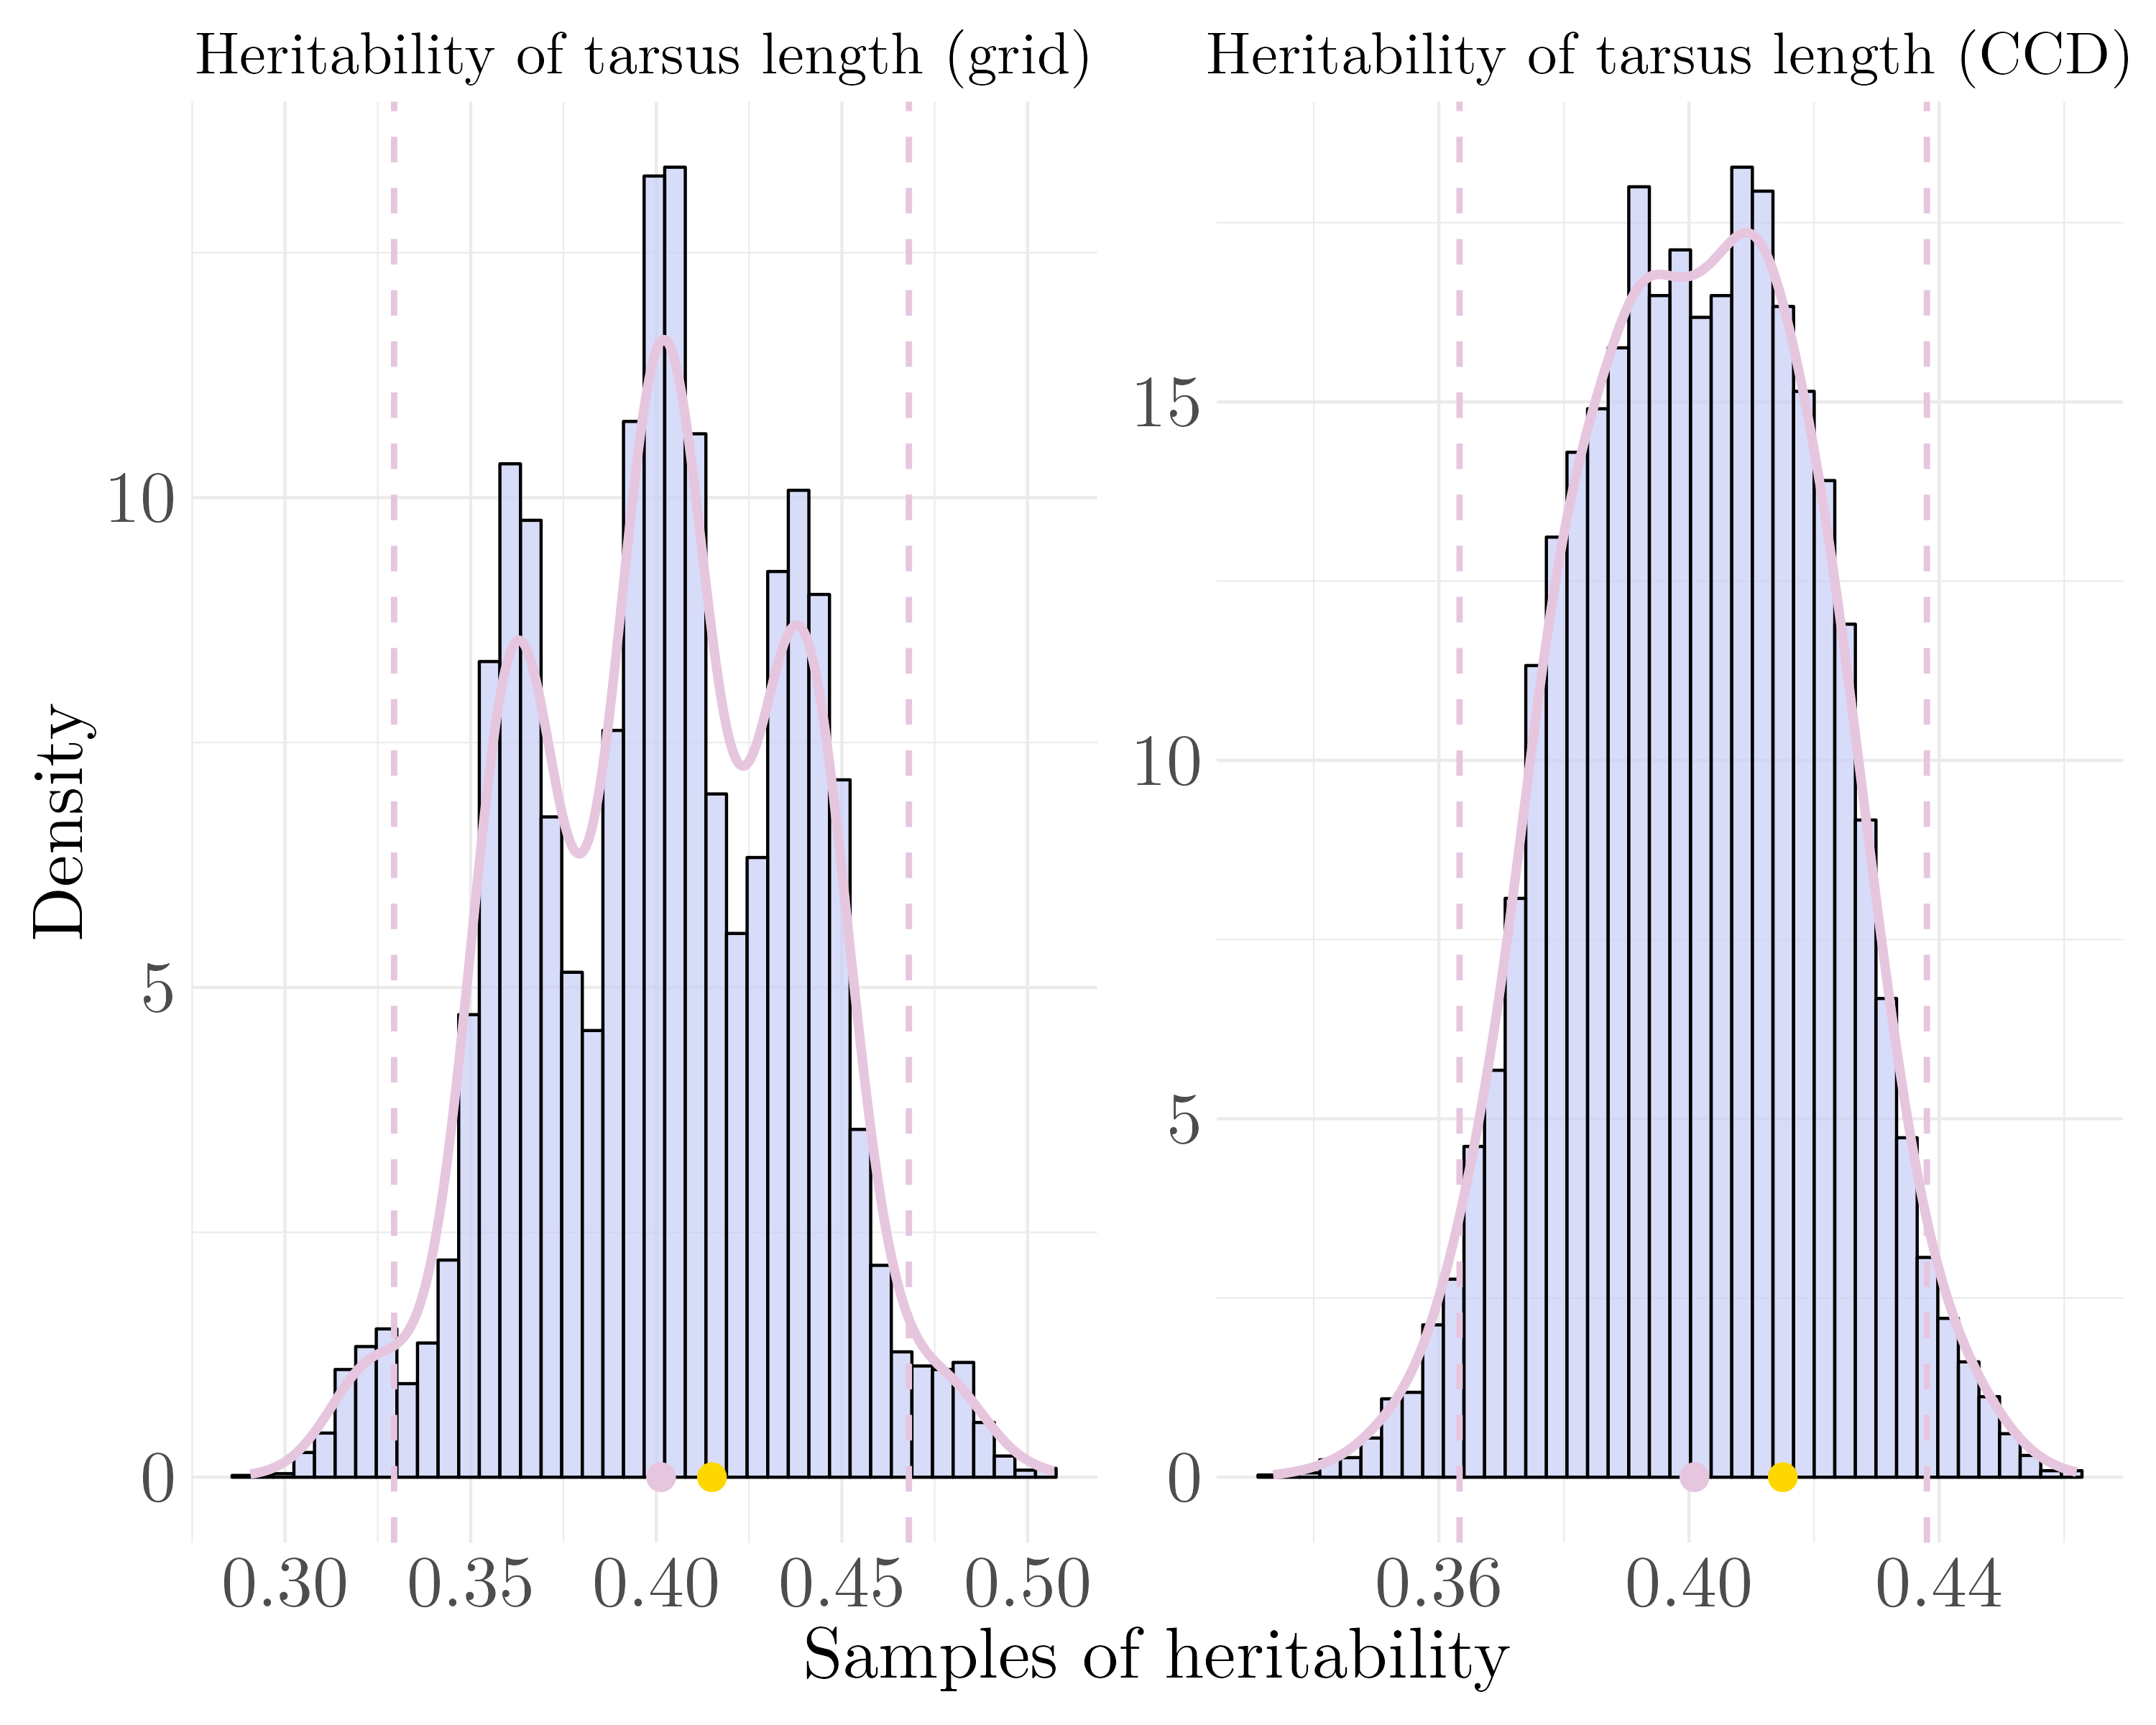
\includegraphics[width=\linewidth]{Figures/House sparrow study/Heritability_tarsus_combined.png}
%   \caption[Estimated heritability of tarsus length]{Histogram showing estimated heritability values for tarsus length of the house sparrows from the BVI method for the grid integration strategy (left) and the CCD integration strategy (right). The two dots at the bottom represent the mean of the samples (pink) and the estimate from \citep{Silva2017} (gold). The dashed lines represent the lower and upper value for the $95\%$ percentile.}
%   \label{fig:heritability_tarsus_combined}
% \end{figure}
\noindent We see in as natural that some patterns in these results are hard to fully interpret, as the dataset is relatively small and from the real world. Further, the measurements are taken on birds that are quite small, so one should expect measurement error to some degree.

% \section{Non-Gaussian simulation study}
% In this section, we display the results of our simulation study of a binomial and a Poisson regression. We note that it has been difficult to find suitable methods to compare the non-Gaussian models with, as we are not aware of any method that calculates relative variable importance for all covariates in the same manner. In parallel to fitting our model as described in \Cref{sec:simulation_study}, we fit a model using the \texttt{rptR} package with $100$ bootstrap samples. This allows us to directly compare the importance of the random effect and the marginal and conditional $R^2$ values. However, it does not compute the importance of each fixed effect.  
\section{Binomial simulation}
In this section, we display the results of our simulation study of a binomial regression on binary responses. We note that it has been difficult to find suitable methods to compare the non-Gaussian models with, as we are not aware of any method that calculates relative variable importance for all covariates in the same manner as the BVI method. In parallel to fitting our model as described in \Cref{sec:simulation_study}, we fit a model using the \texttt{rptR} package with $100$ bootstrap samples. This allows us to directly compare the importance of the random effect and the marginal and conditional $R^2$ values. However, it does not compute the importance of each fixed effect. The model to be analysed is the binomial regression on binary response, modeled with the logit-link function. As mentioned, we fit \( N_{\text{sim}} = 500 \) models for each correlation level using the Bayesian Variable Importance method. Then, the BVI method extracts the posterior modes and calculates the derived measures as described in \Cref{ch:method} to estimate the mode of relative importance for all covariates in each model. A summary of the 500 estimated modes is shown in the supplementary material (\Cref{ap:supplementary}, specifically \Cref{table:summary_logit}), which contains the mean value and values for the lower and upper $95$th quantile.
% The first model to be analysed is the binomial regression on binary response, modelled with the logit-link function. As mentioned, we fit $N_{sim}=500$ models for each correlation level using the Bayesian Variable Importance method. Then, the BVI method extracts the posterior mode, and calculates the derived measures as described in \Cref{ch:method} to estimate the mode of relative importance for all covariates in each model. A summary of the $500$ estimated modes are shown in the supplementary material (\Cref{ap:supplementary}, specifically \Cref{table:summary_logit}), which contains the mean and values for the lower and upper $95\%$ quantile.
\subsection{Fixed effects}
The sampled distribution for the posterior modes of relative importance allocated to the three fixed effects $X_1, X_2$ and $X_3$ are shown for each correlation level (\Cref{fig:fixed_combined_logit}). We see that the distributions generally form a normal shape around the mean, with somewhat varying spread. As correlation levels go from negative to positive, meaning that the variance contribution from the fixed effects increase, the importances of the fixed effects also increase. This is expected, as the marginal $R^2$ increases and is spread across the correlated fixed effects. The difference is quite substantial, with the average relative importance allocated to $X_1$ for $\rho=-0.4$ being $0.020$ compared to $0.173$ for $\rho=0.4$. The same pattern is seen for $X_2$ and $X_3$, with the average relative importance increasing from $0.077$ to $0.239$ for $X_2$ and from $0.166$ to $0.299$ for $X_3$ when going from $\rho=-0.4$ to $\rho=0.4$. For $\rho=0$ (middle plot of \Cref{fig:fixed_combined_logit}), it is clear that the average estimate for relative importance of all fixed effects is very similar to the expected importance (\Cref{table:3}) shown as a dashed green line. 
\\
\\
We notice that the covariates $X_1$ and $X_2$ are allocated a significantly larger share when correlation goes from $\rho=0$ to $\rho=0.4$, whereas $X_3$ is almost unchanged for the same correlation levels. This was also experienced in the simulation study on LMMs in \Cref{sec:simulation_study_gauss} from \citet{Arnstad:Relative_variable_importance_in_Bayesian_linear_mixed_models:2024}. It is explained by the fact that off-diagonal elements of $\boldsymbol{\Lambda}$ increase positively when the fixed effects are positively correlated, while the diagonal elements decrease. In the uncorrelated case, $\boldsymbol{\Lambda}$ should be equal to the identity matrix. The squared columns of $\boldsymbol{\Lambda}$ sum to one and act as weights. Due to this weighting, when $\rho=0.4$, $X_1$ will receive an importance estimate where $\beta_2^2$ and $\beta_3^2$ will have positive weights contrary to $\rho=0$ where the only weight is put on $\beta_1^2$. Since $\beta_1^2$ is smaller than $\beta_2^2$ and $\beta_3^2$, the higher positive correlation level yields a higher importance estimate for $X_1$. The same pattern is seen for $X_2$, where $\beta_1^2$ is smaller and $\beta_3^2$ is larger than $\beta_2^2$. This means the importance of $X_2$ is estimated to be higher for $\rho=0.4$ than for $\rho=0$, but the increase is smaller than the increase for $X_1$ \citep{Arnstad:Relative_variable_importance_in_Bayesian_linear_mixed_models:2024}. In contrast, the importance of $X_3$ is then estimated with more weight on $\beta_1^2$ and $\beta_2^2$, which are both smaller than $\beta_3^2$, and thus the importance is not notably increased. If one had introduced a larger positive correlation level than $\rho=0.4$, we would therefore expect the importance of $X_3$ to even decrease, as was seen in \citet{Arnstad:Relative_variable_importance_in_Bayesian_linear_mixed_models:2024}. It is hard to say, based on these results, whether the inverse pattern can be seen for negative correlation levels, but it could be noted that the decrease in importance is less for $X_3$ compared to $X_1$ and $X_2$ when $\rho$ changes from $0$ to $-0.1$.
\\
\\
Generally, it seems that the method is able to capture the expected effects of varying correlation levels, and is in close agreement with the expected theoretical values when the fixed effects are uncorrelated. 
\begin{figure}[H]
  \centering
  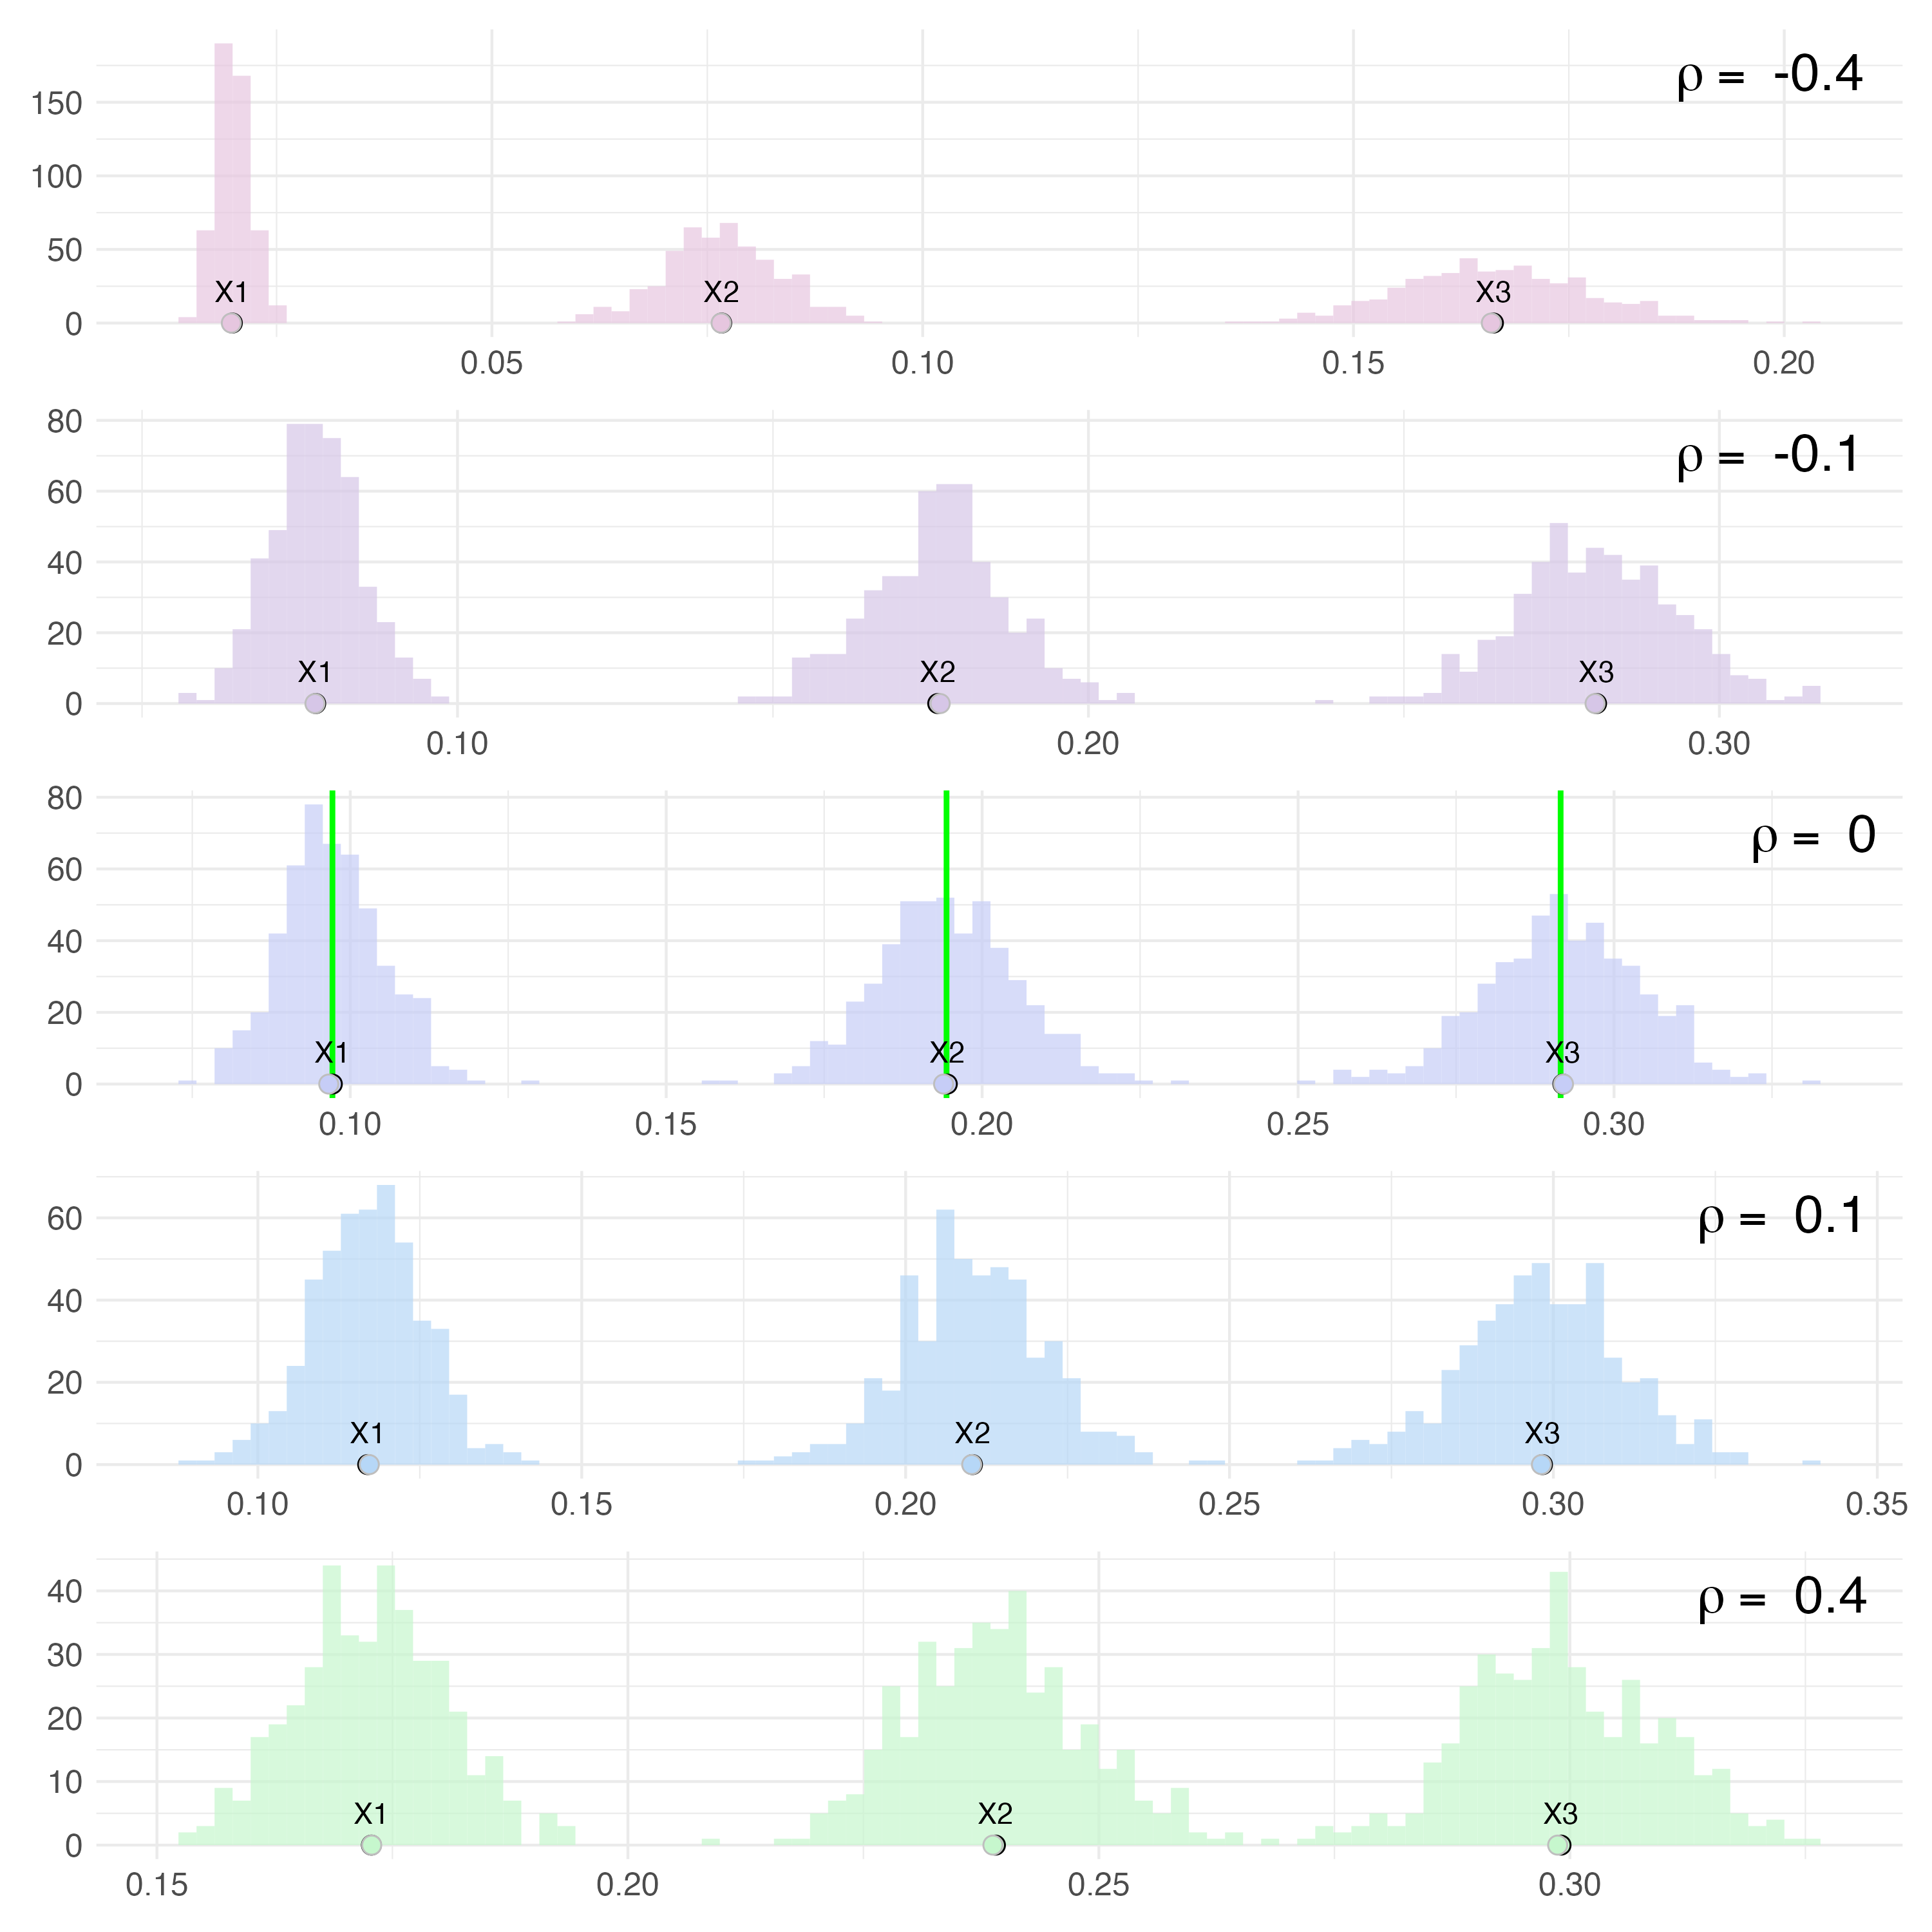
\includegraphics[width=1\linewidth]{Figures/Simulation study/Fixed_combined_logit.png}
  \caption[Relative importance of the fixed effects in binomial GLMM]{Histogram with the distribution of posterior modes of relative importance for the fixed effects present in the binomial regression for the different correlation levels $\rho$. The modes of relative importance are calculated by the Bayesian Variable Importance method from the $N_{\text{sim}}=500$ models fit in the simulation study. The vertical green line for $\rho=0$ displays the expected relative importance in the case of uncorrelated data. The mean of the mode values for all simulations is denoted at the bottom of each histogram as a circle.}
  \label{fig:fixed_combined_logit}
\end{figure}
  %\label{fig:fixed_effects_logit}
%\end{figure}
\subsection{Random effect}
The sampled posterior modes of importances for the random effect in the logit model all seem to be roughly normally distributed around the mean (\Cref{fig:relimp_random_logit}). The spread of the random effects seem to be larger than the spread seen in the fixed effects for negative correlations, and more similar for independent and positively correlated covariates. One can see that when the correlation in fixed effects go from negative to positive, the estimated importance of the random effect shrinks. Specifically, when $\rho=-0.4$ the average estimate of relative importance for the random effect is $0.171$ compared to only $0.067$ when $\rho=0.4$. This naturally occurs as the variance contribution from the random effect should be held constant for the correlation levels, and the variance contribution from the fixed effects rise as the correlation increases. Therefore, the proportion of variance explained, which is our definition of relative variable importance, will decrease for the random effect. For $\rho=0$ we see that the average relative importance estimate lies very near the expected value of $0.097$ (\Cref{table:3}). The orange dot at the bottom of the histograms in \Cref{fig:relimp_random_logit} displays the estimated relative importance of the fixed effect from the \texttt{rptR} package, and we see that the estimates are quite close to the mean of the BVI method. The largest difference from the BVI and the \texttt{rptR} package is $0.021$ and are found when $\rho=0$. This difference is $22\%$ of the average estimated relative importance from the BVI method, and is therefore not negligible. However, the methods seem to be in agreement for the overall trends and the methods are closer in accordance with each other for the other correlation levels.
\\
\\
\begin{figure}[ht]
  \centering
    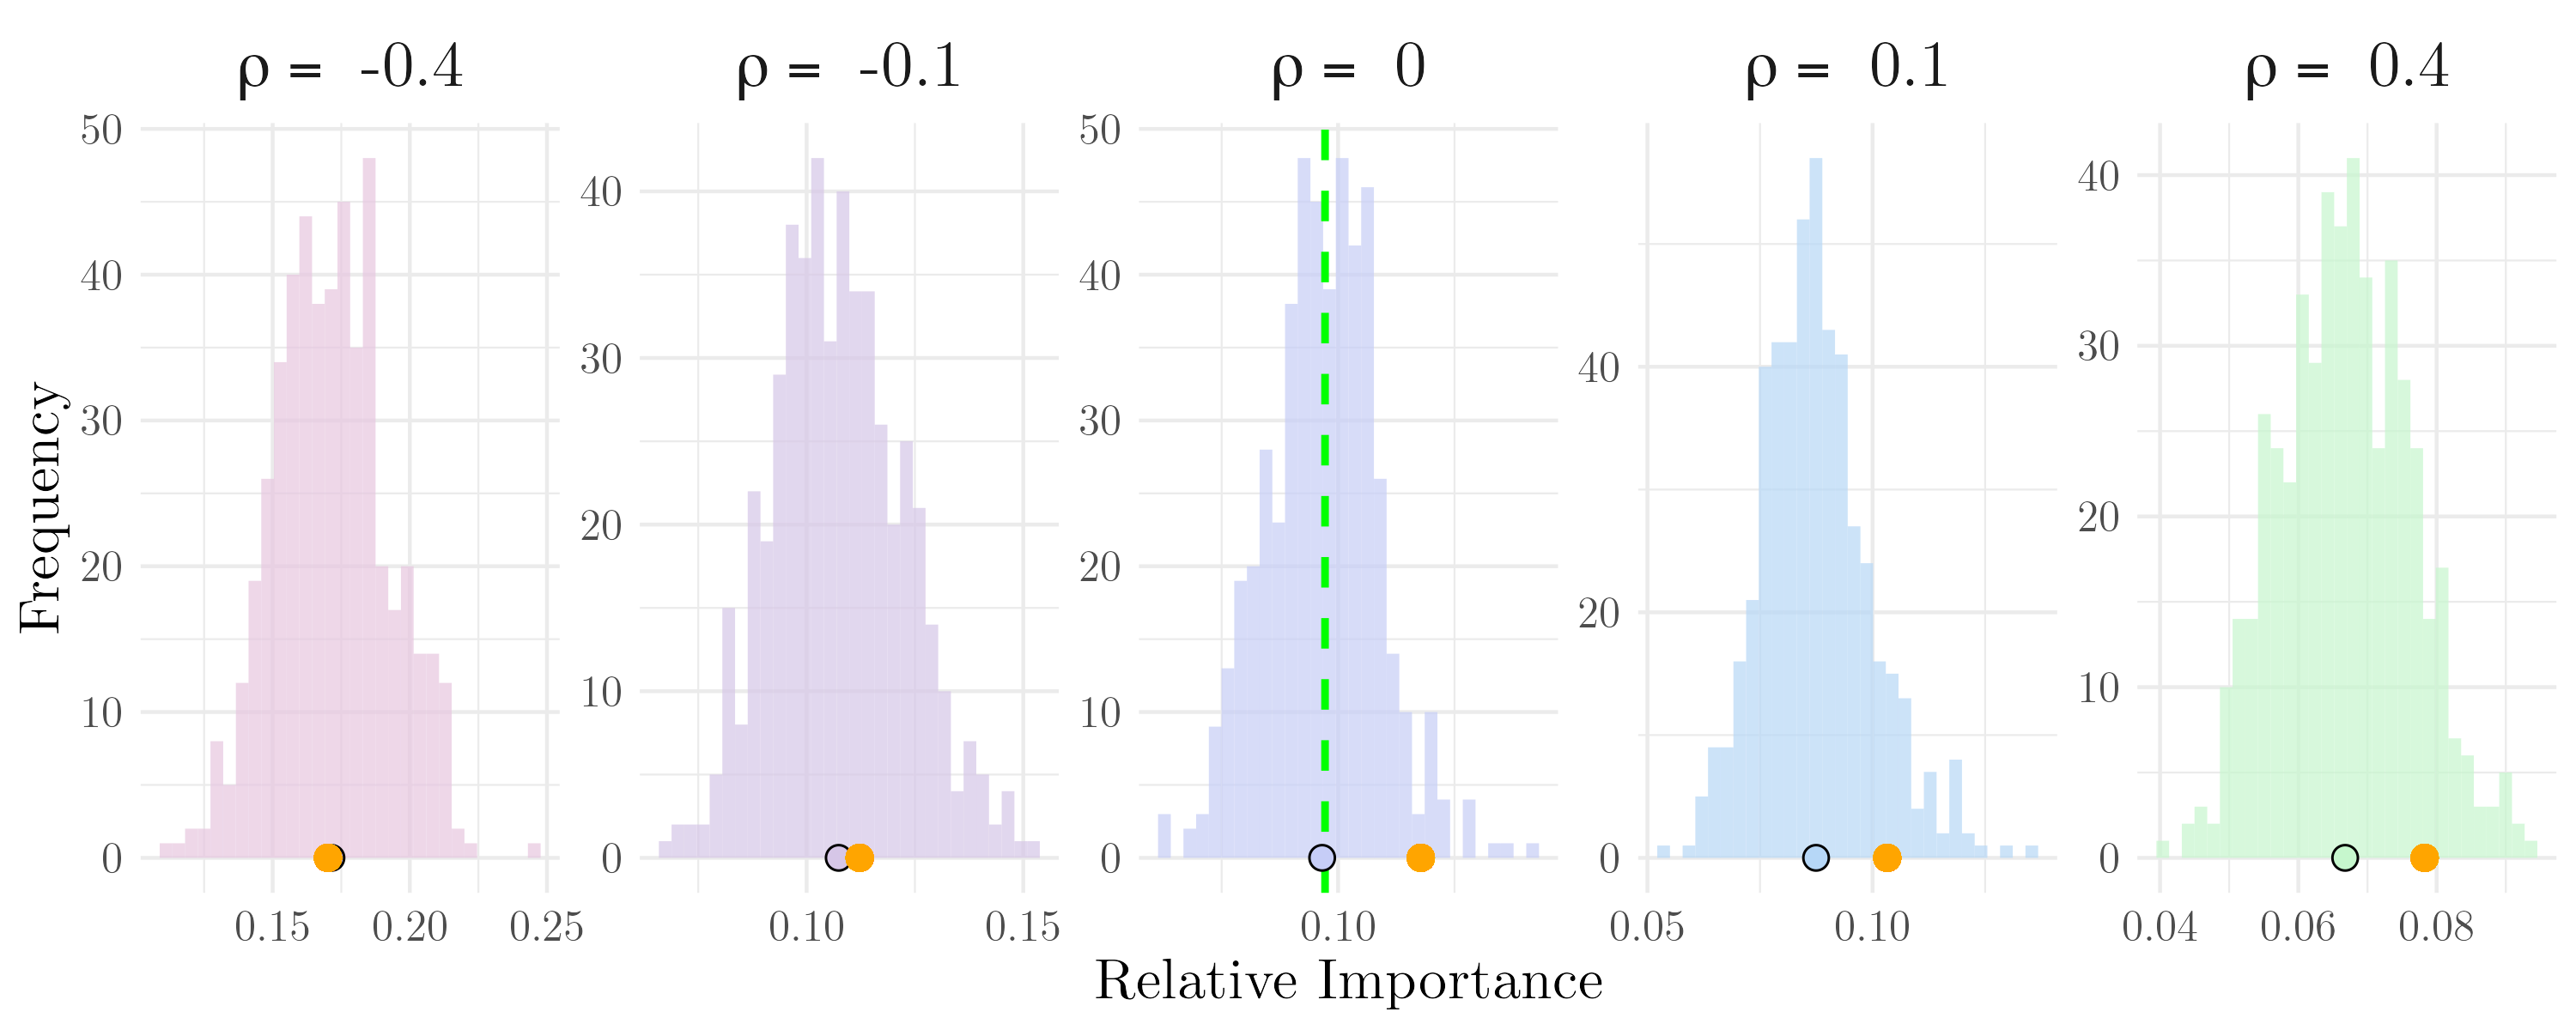
\includegraphics[width=1\linewidth]{Figures/Simulation study/Random_logit.png}
    \caption[Relative importance of the random effect $\boldsymbol{\alpha}$ in binomial GLMM]{Histogram with the posterior modes of the binomial regression from the BVI method for each of the $N_{\text{sim}}=500$ models fit, estimating relative importance of the random effect $\boldsymbol{\alpha}$ across the different correlation levels $\rho$. The mean of the mode values from all simulations is displayed at the bottom as a circle and the orange dot at the bottom displays the estimate from the \texttt{rptR} package. The vertical green line for $\rho=0$ is the expected relative importance as in \Cref{table:3}.}
    \label{fig:relimp_random_logit}
\end{figure}
\subsection{\texorpdfstring{$R^2$}{Lg} estimates}
An important measure in this simulation study is the modes for the sampled posterior distribution of marginal and conditional $R^2$ (\Cref{fig:r2_combined_logit}). The expected values for the marginal and conditional $R^2$ are shown in \Cref{table:r2values}, and are displayed as vertical green lines in each plot. It is clear that, regardless of correlation level, the BVI method is able to estimate the marginal and conditional $R^2$ close to what we expect. The distributions of $R^2$ values seem to have the shape of a bell curve and are symmetric around the mean value. The spread is naturally larger than for the individual fixed effects and random effects, as the $R^2$ is constructed from these importances. For both the marginal and conditional $R^2$ estimates, there is only a negligible difference between the results from the BVI method and the expected values. When comparing to the results from the \texttt{rptR} package, there are some larger differences. The marginal $R^2$ deviates the most when $\rho=0$ with a difference of $0.014$, which is $3\%$ of the average estimated value. For the conditional $R^2$ the largest difference is $0.018$ which also makes up $3\%$ of the average estimated value, found for $\rho=0.1$. Generally, the BVI method seems to be in line with our expectation for $R^2$ values, deviating slightly more from the \texttt{rptR} package estimates.
\begin{figure}[H]
  \centering
  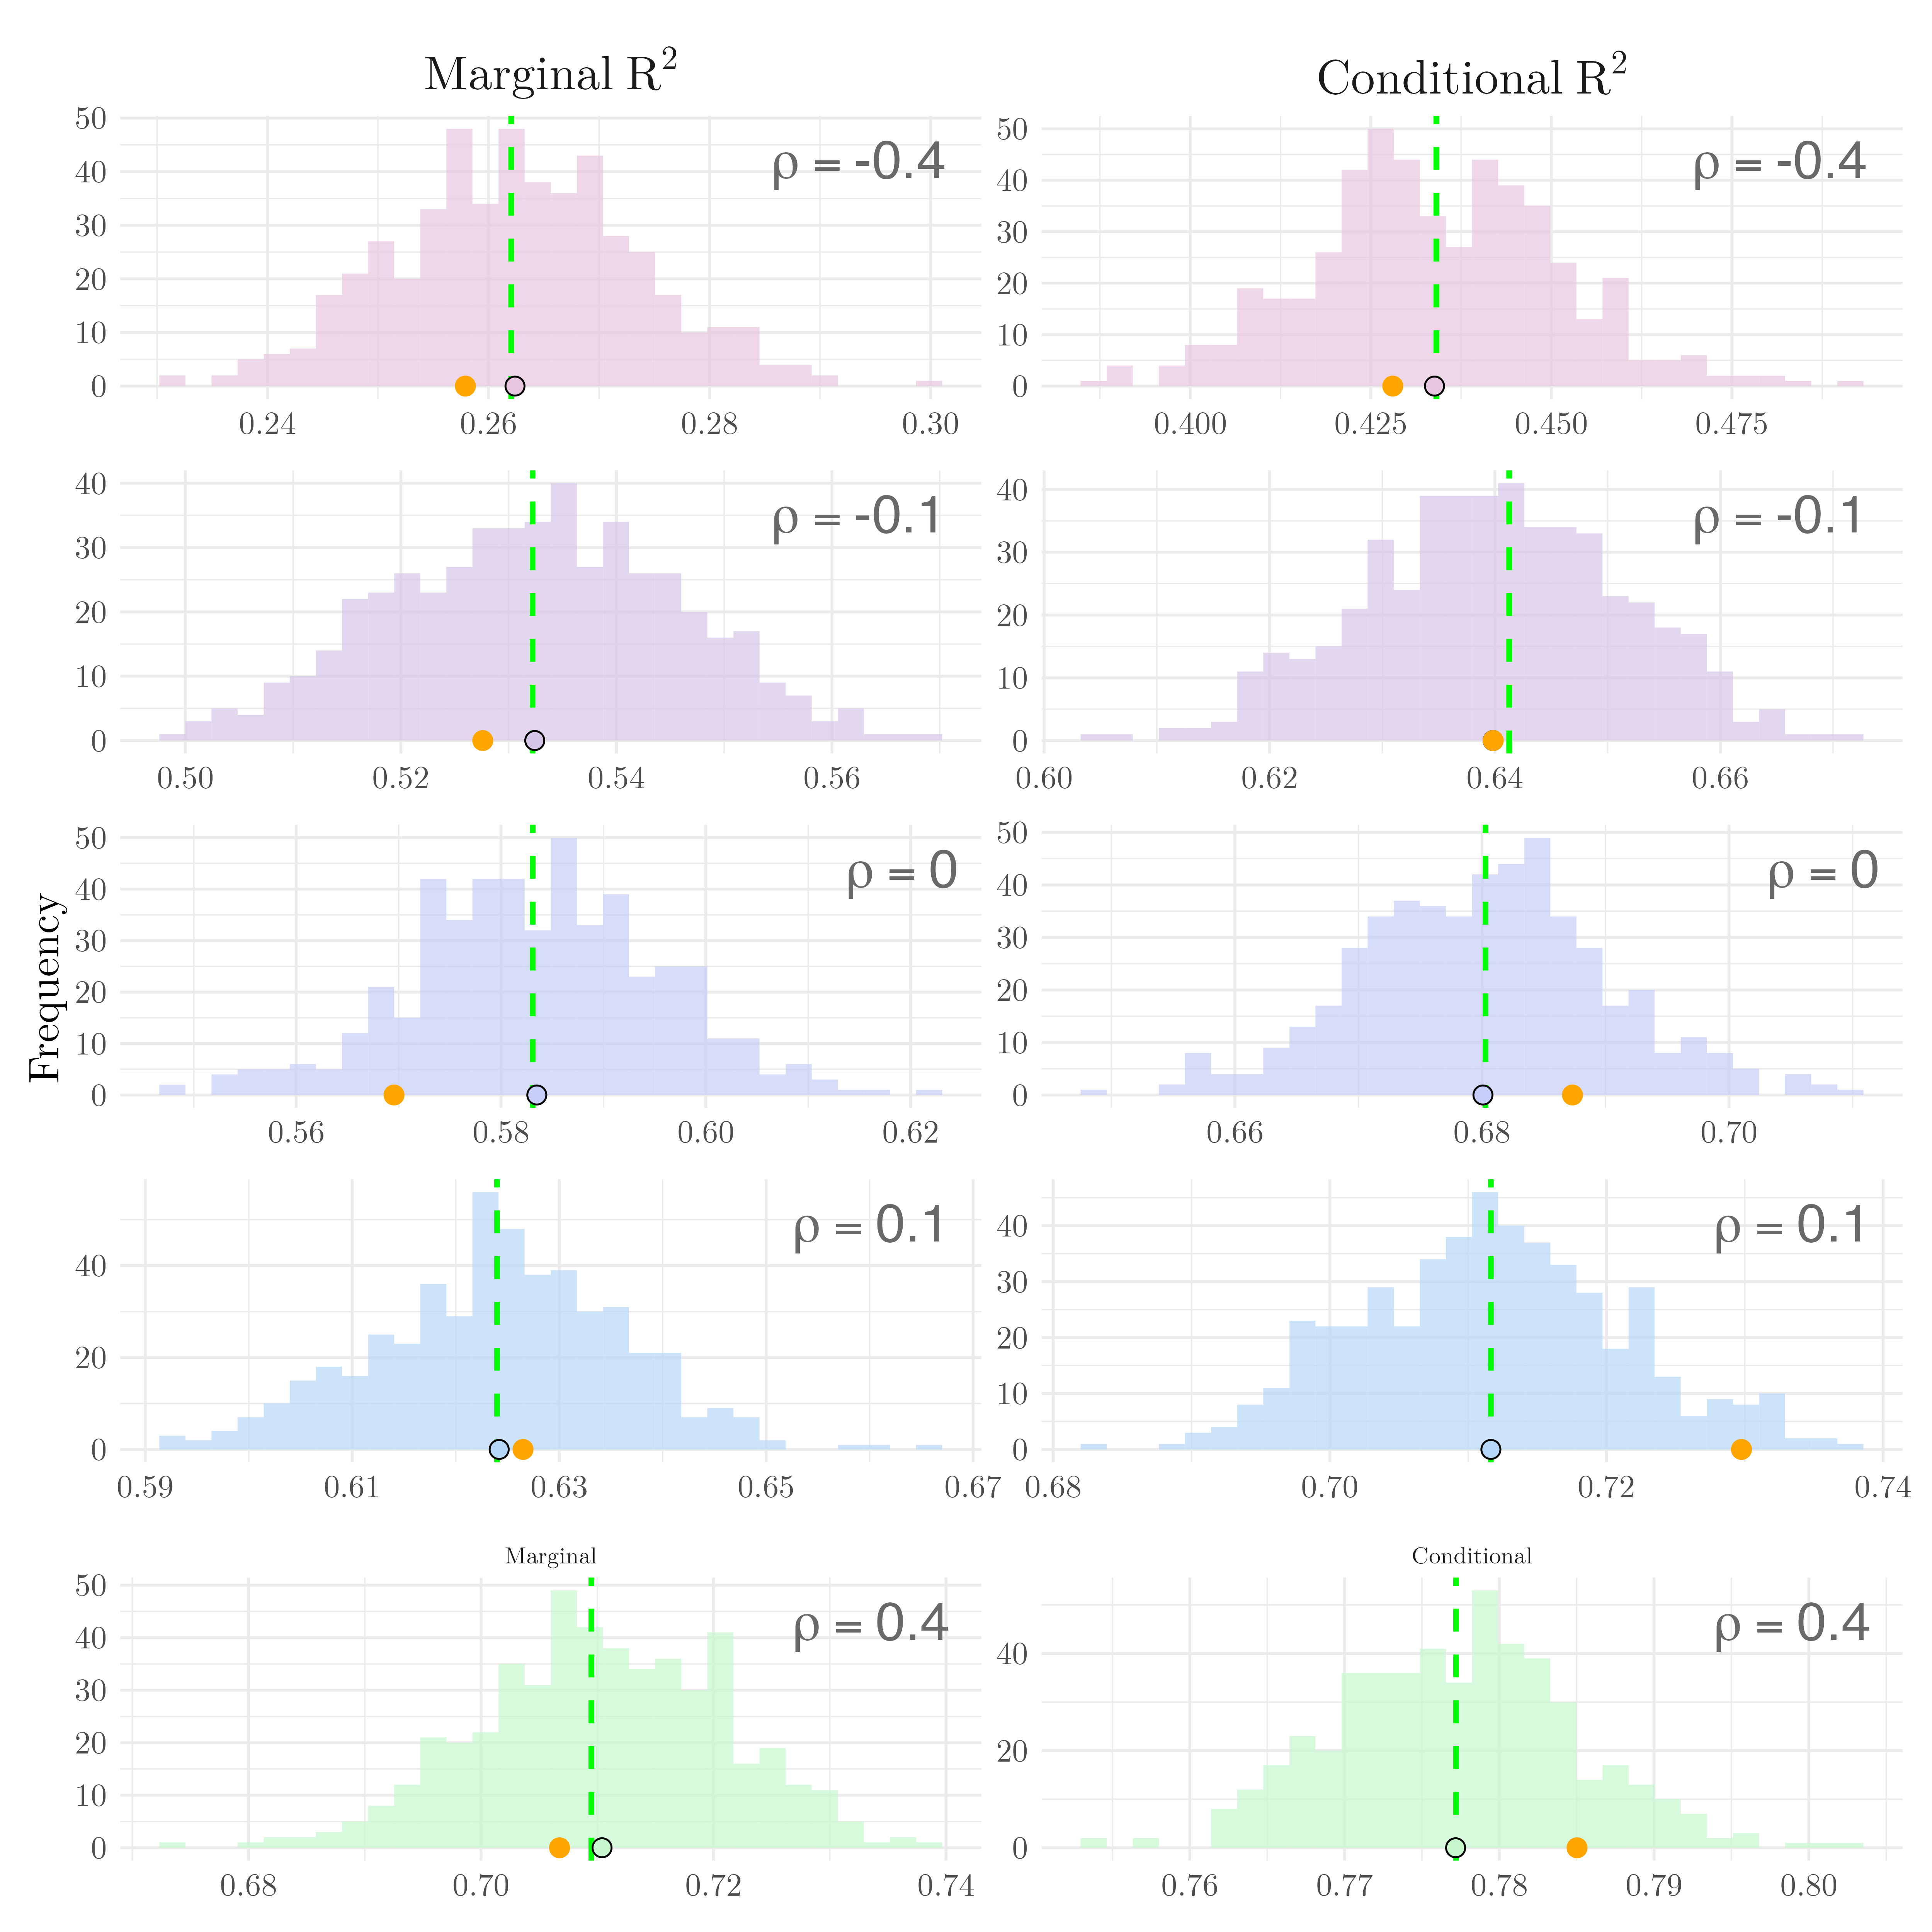
\includegraphics[width=1\linewidth]{Figures/Simulation study/R2_combined_logit.png}
  \caption[Marginal and conditional $R^2$ in binomial GLMM]{Histograms with the posterior modes of the estimated marginal and conditional $R^2$ from the BVI method for the binomial regression for the different correlation levels $\rho$. The posterior modes are calculated by the Bayesian Variable Importance method from the $N_{\text{sim}}=500$ models fit in the simulation study. The expected values are displayed as vertical green lines, and can be found in \Cref{table:r2values}, while the orange dot denotes the estimate from the \texttt{rptR} package. The mean value of the $R^2$ modes for all simulations is marked with a circle at the bottom of each histogram.}
  \label{fig:r2_combined_logit}
\end{figure}
\section{Poisson simulation}
In this section, we present the results of our simulation study of a Poisson regression. Similar to the binomial regression, we faced challenges in finding suitable methods for comparison. To address this, the \texttt{rptR} package was used with $100$ bootstrap samples, which provided comparable measures in some instances. This approach allowed us to compare the importance of the random effect and the marginal and conditional \( R^2 \) values; however, \texttt{rptR} does not provide the importance of each fixed effect. We modeled the Poisson regression with count responses using the log-link function. The Poisson models were fit with the same correlation levels as the binomial simulation and $N_{\text{sim}}=500$ models for each level were fitted. For each fitted model, the Bayesian Variable Importance method was employed to extract the posterior mode and then calculate the relative variable importance measures as described in \Cref{ch:method}. In the supplementary material (\Cref{ap:supplementary}, specifically \Cref{table:summary_poisson}), a summary of the mean and $95$th quantile values of the $500$ importance estimates for different correlation levels is given.
\subsection{Fixed effects}
As for the binomial model, we first look at the fixed effects. The estimates of posterior modes for relative importance for the fixed effects (\Cref{fig:fixed_combined_poisson}) are very similar in shape as the binomial model. Again, the spread is somewhat varying for the different correlation levels. Overall, the estimates for the Poisson model are marginally smaller than the binomial for negative correlations, and marginally larger for positive correlations. This is mainly due to the log-link having a distributional variance which is dependent on the correlation of covariates, and the logit-link having a constant distributional variance. When covariates are negatively correlated, the distributional variance of the log-link increases and the importance allocated to covariates decreases. Similarly, the opposite happens when covariates are positively correlated. The quantiles of the Poisson model is marginally more narrow than that of the binomial model. It seems the estimates form a normal curve about the mean, and for $\rho=0$ the average estimated importance is close to the expected value. The same influence of varying correlation levels can be seen as in the binomial model, namely that we obtain larger importance of the fixed effects when the correlation increases. Again the difference is notably large, with the average relative importance of $X_1$ going from $0.017$ for $\rho=-0.4$ to $0.181$ for $\rho=0.4$. For $X_2$ and $X_3$ the average relative importance for the same correlation levels increases from $0.066$ to $0.251$ and from $0.143$ to $0.314$ respectively.
\\
\\
Further, we see the same pattern of larger increase in importance to $X_1$ than for $X_2$ and larger for $X_2$ than $X_3$, as for the binomial model, when correlation increases from $\rho=0$ to $\rho=0.4$. Specifically, $X_1$ increases with $0.084$, $X_2$ with $0.058$ and $X_3$ with $0.024$ when we go from uncorrelated covariates to the highest correlation level. This is in line with our expectations, as the diagonal elements of $\boldsymbol{\Lambda}$ decrease with increasing correlation levels and the off-diagonal elements increase. The inverse pattern is once again not so clear, as the decrease of $X_3$ is in fact larger than the decrease of $X_1$ and $X_2$. However, if one looks at the relative decrease in importance, it is clear that the decrease is larger for $X_1$ and $X_2$ than for $X_3$ when going from $\rho=0$ to $\rho=-0.4$. The inverse pattern may therefore be hard to detect, due to the relatively large difference in magnitude of the coefficients. For the case $\rho=0$, we see that the mean of our samples coincides with the expected relative importance (\Cref{table:3}), and it seems the model express the expected pattern of relative importance for varying correlation levels.
\begin{figure}[H]
  \centering
  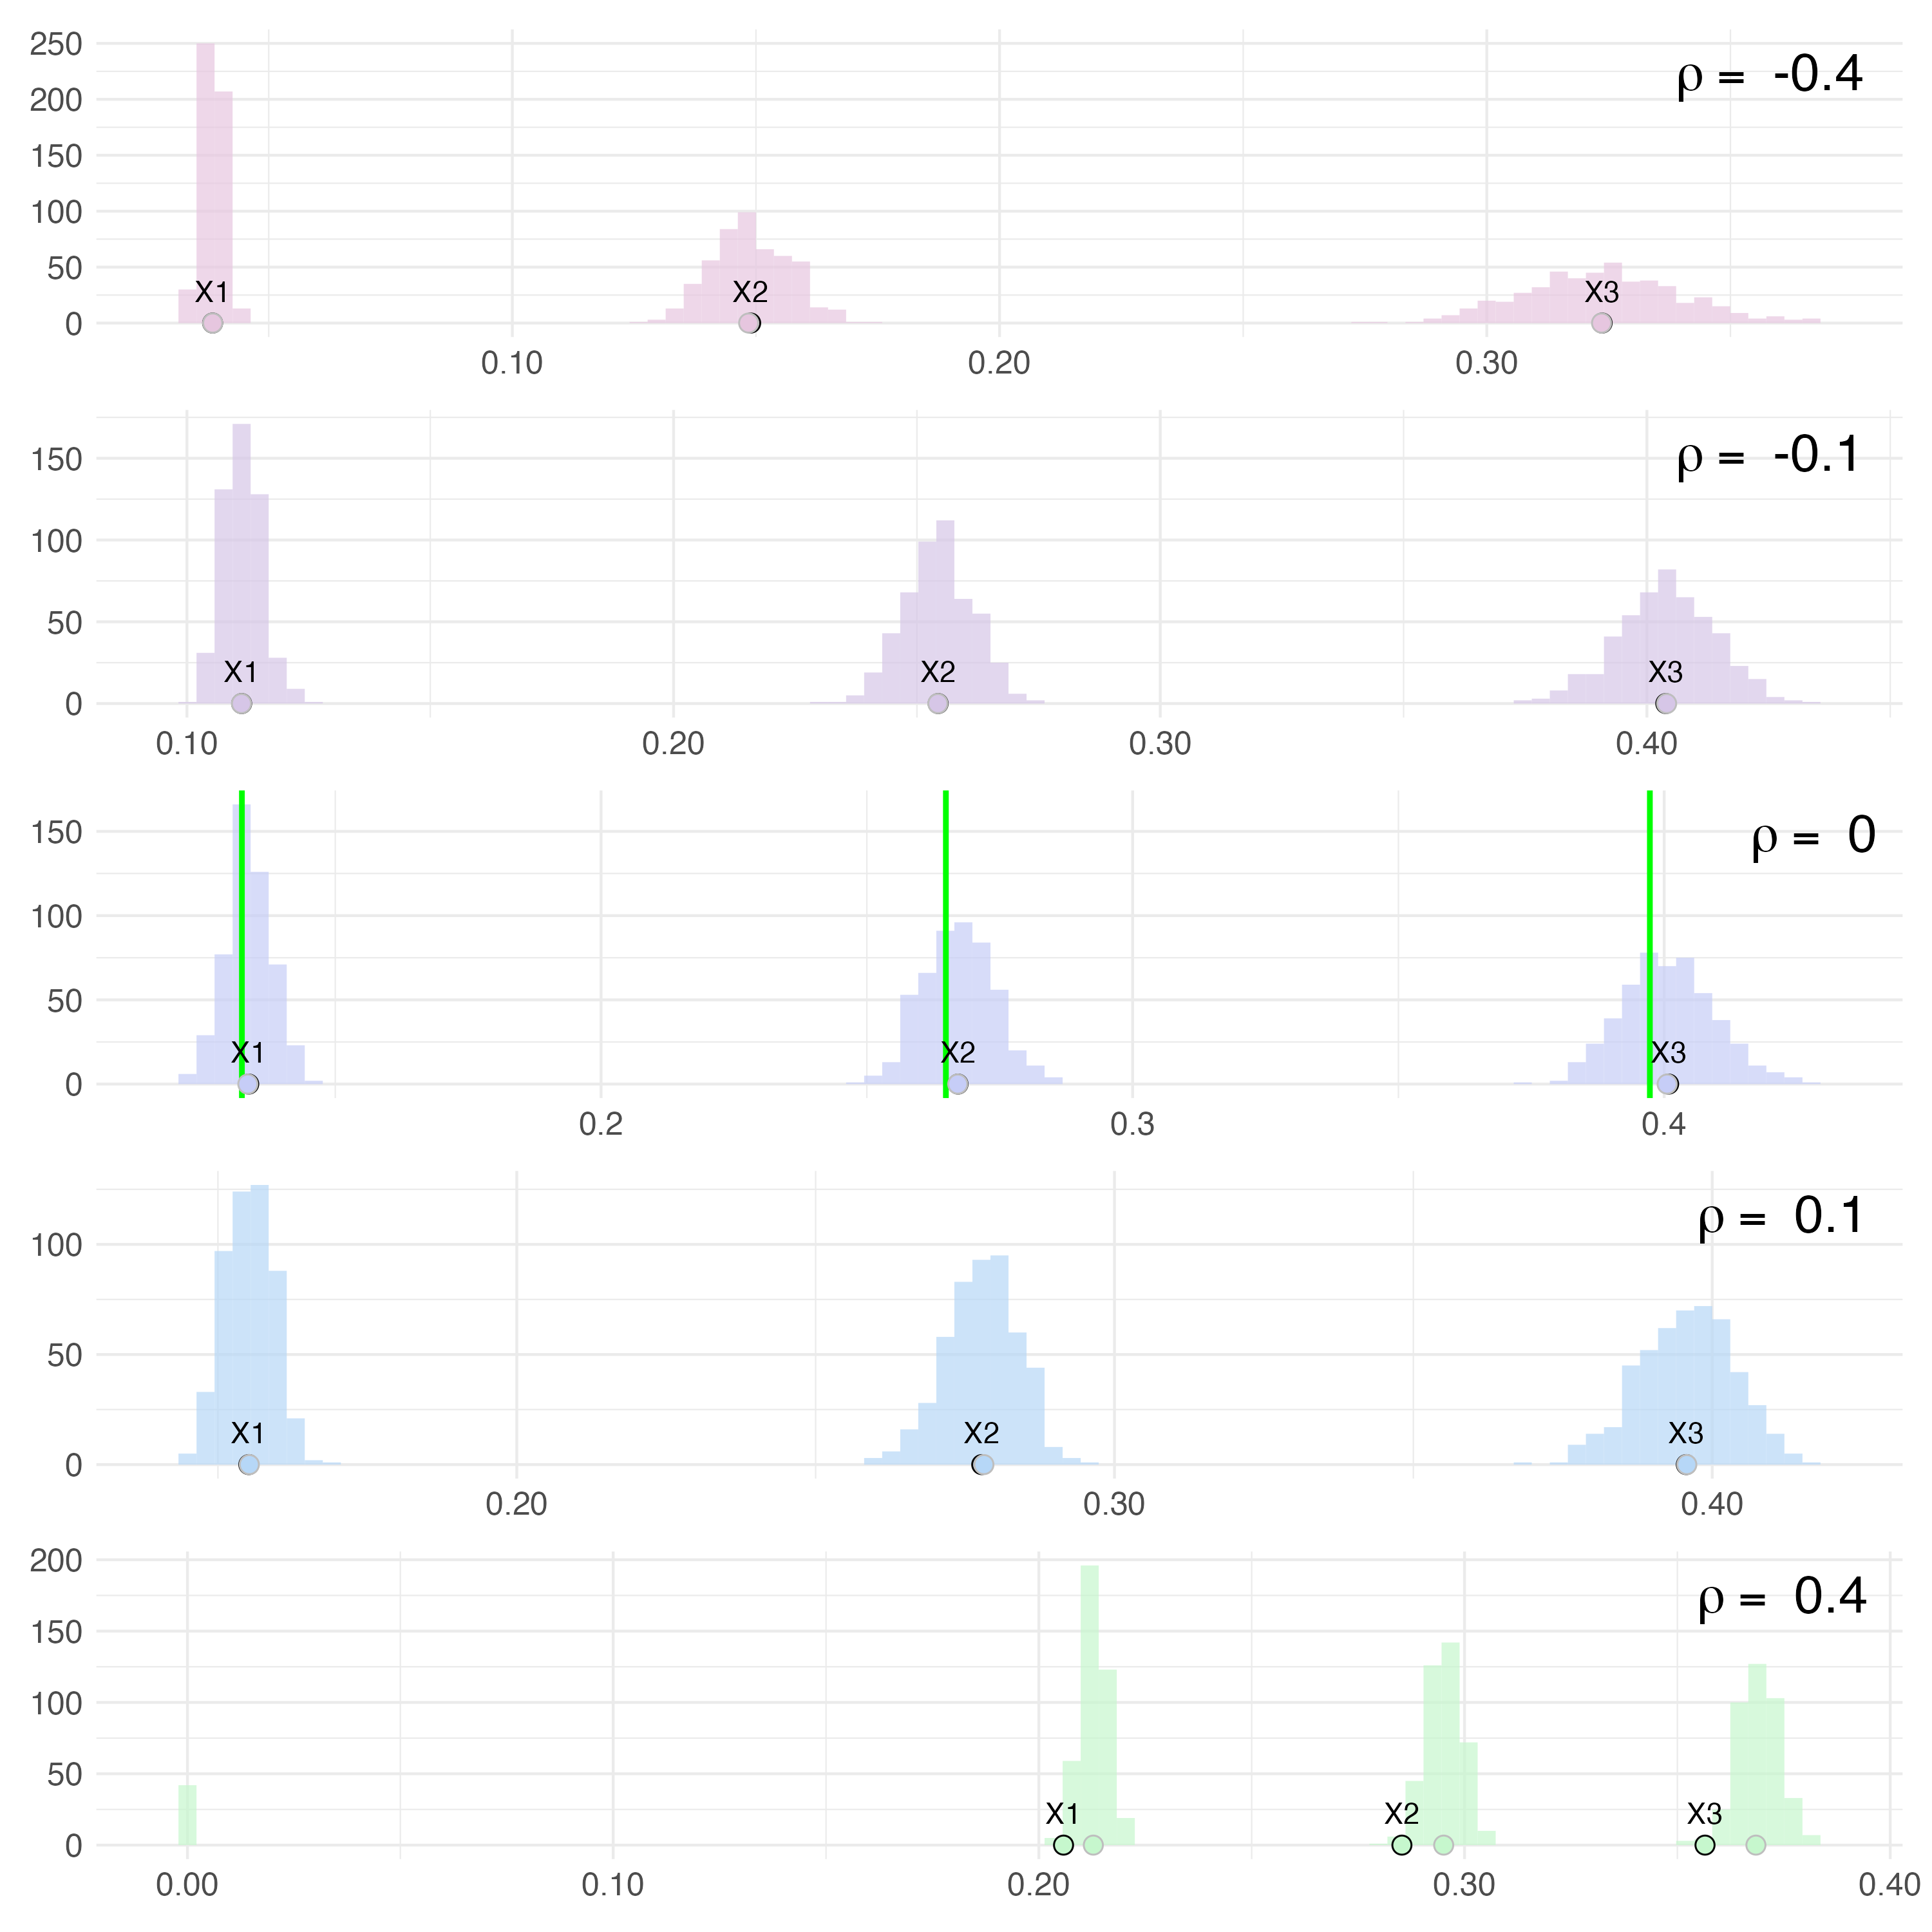
\includegraphics[width=1\linewidth]{Figures/Simulation study/Fixed_combined_poisson.png}
  \caption[Relative importance of the fixed effects in Poisson GLMM]{Histogram with the posterior modes of relative importance of the fixed effects present in the Poisson regression for the different correlation levels $\rho$. The modes are calculated by the Bayesian Variable Importance method from the $N_{\text{sim}}=500$ models fit in the simulation study. The vertical green line for $\rho=0$ displays the expected relative importance in the case of uncorrelated data, and the mean of the modes for all simulations is denoted at the bottom of each histogram as a circle.}
  \label{fig:fixed_combined_poisson}
\end{figure}
\subsection{Random effect}
When looking at the sampled posterior distribution of relative importance estimates of the random effect in the Poisson model (\Cref{fig:relimp_random_poisson}), we see that they too are generally smaller than the same estimates for the binomial case when covariates are negatively correlated. Conversely, for positive correlations, the estimates tend to be marginally larger. This is consistent with the pattern observed for the fixed effects, and caused by the distributional variance of the log-link being dependent on the correlation of covariates. Furthermore, the distributions of relative importance allocated to the random effect for different correlation levels all appear to be normal and symmetric about the mean. We notice a somewhat larger spread in the random effect importances than in the fixed effect importances for the Poisson model. The shrinkage effect of increasing correlation is also here apparent, with the average relative importance of the random effect going from $0.149$ for $\rho=-0.4$ to $0.072$ for $\rho=0.4$. We again emphasize that this is natural and anticipated, as the random effect variance is constant across correlation levels, while the variance of the fixed effects varies. The expected value when $\rho=0$ is $0.097$ as shown in \Cref{table:3}, and we see that the average estimate is close to this value. The orange dots, denoting the estimates from the \texttt{rptR} package, are close to the average estimate from the BVI method, with the largest difference being $0.017$ for $\rho=0.4$. This is also the largest relative difference, being $24\%$ of the average estimated relative importance. The BVI method seems to be in agreement with the expected values for the relative importance of the random effect, and the \texttt{rptR} estimates are fairly close to the BVI method.
\begin{figure}[H]
  \centering
    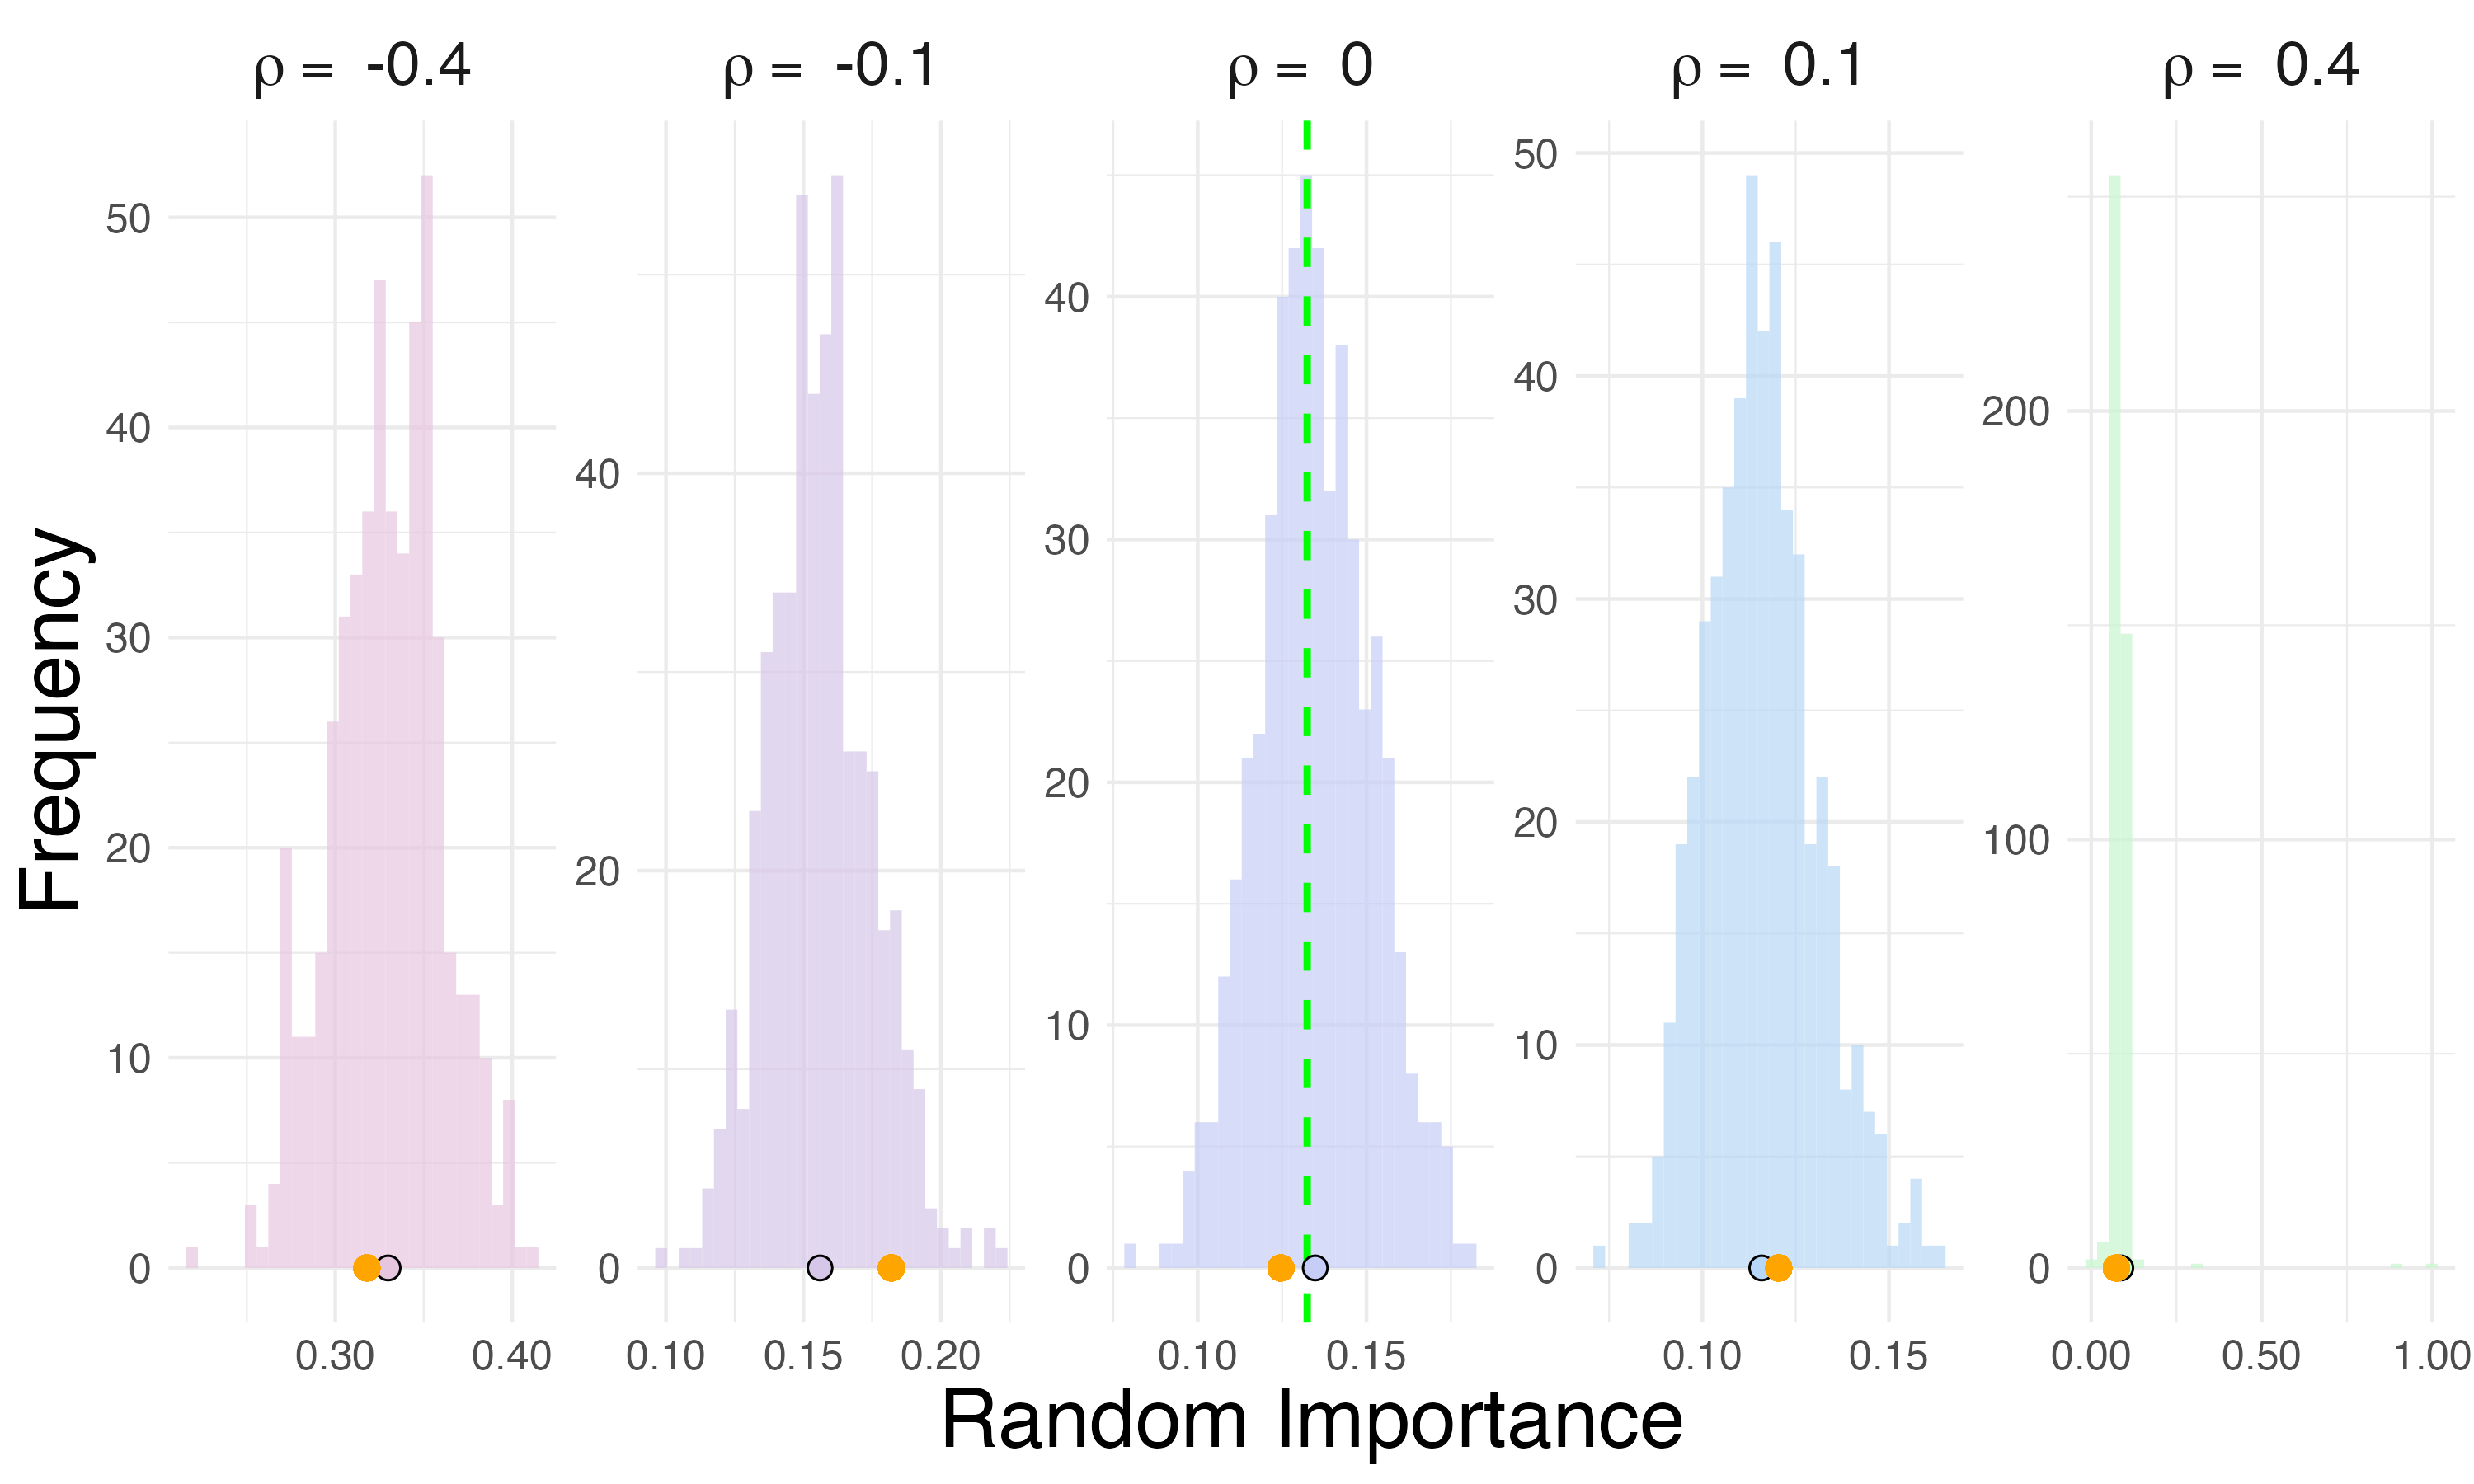
\includegraphics[width=1\linewidth]{Figures/Simulation study/Random_poisson.png}
    \caption[Relative importance of the random effect $\boldsymbol{\alpha}$ in Poisson GLMM]{Histogram with posterior modes of the relative importance estimates for the random effect $\boldsymbol{\alpha}$ for varying values of $\rho$ in the Poisson regression, calculated by the BVI method. The study conducted $N_{\text{sim}}=500$ simulations and the mean of the modes of relative importance for all simulations is displayed at the bottom of each histogram as a circle. The vertical green line for $\rho=0$ is the expected relative importance as in \Cref{table:3} and the orange dot is the corresponding estimate from the \texttt{rptR} package.}
    \label{fig:relimp_random_poisson}
\end{figure}
\subsection{\texorpdfstring{$R^2$}{Lg} estimates}
Moving on to the estimated posterior $R^2$ distributions for the Poisson model (\Cref{fig:r2_combined_poisson}), we see that the expected values from \Cref{table:r2values} are in close agreement with the average marginal and conditional $R^2$ estimated from the BVI method for all correlation levels. The largest difference in expected values and average values from the BVI method is found for $\rho=0$ and is $0.001$ for the marginal and for the conditional $R^2$ the difference is negligible. The $R^2$ distributions seem roughly normal and symmetric around the mean value, with a plausible size of the spread. Again, there are some more notable differences between the BVI method and the \texttt{rptR} package. For $\rho=0.1$ we observe the difference to be $0.010$ for the marginal $R^2$ and for the conditional $R^2$ when $\rho=-0.4$ it is also $0.010$. These differences are $2\%$ and $4\%$ of the average estimated values, respectively. In general, we also see here that our method aligns closely with our expectation, and deviates a bit more from the \texttt{rptR} package estimates.
\begin{figure}[H]
  \centering
  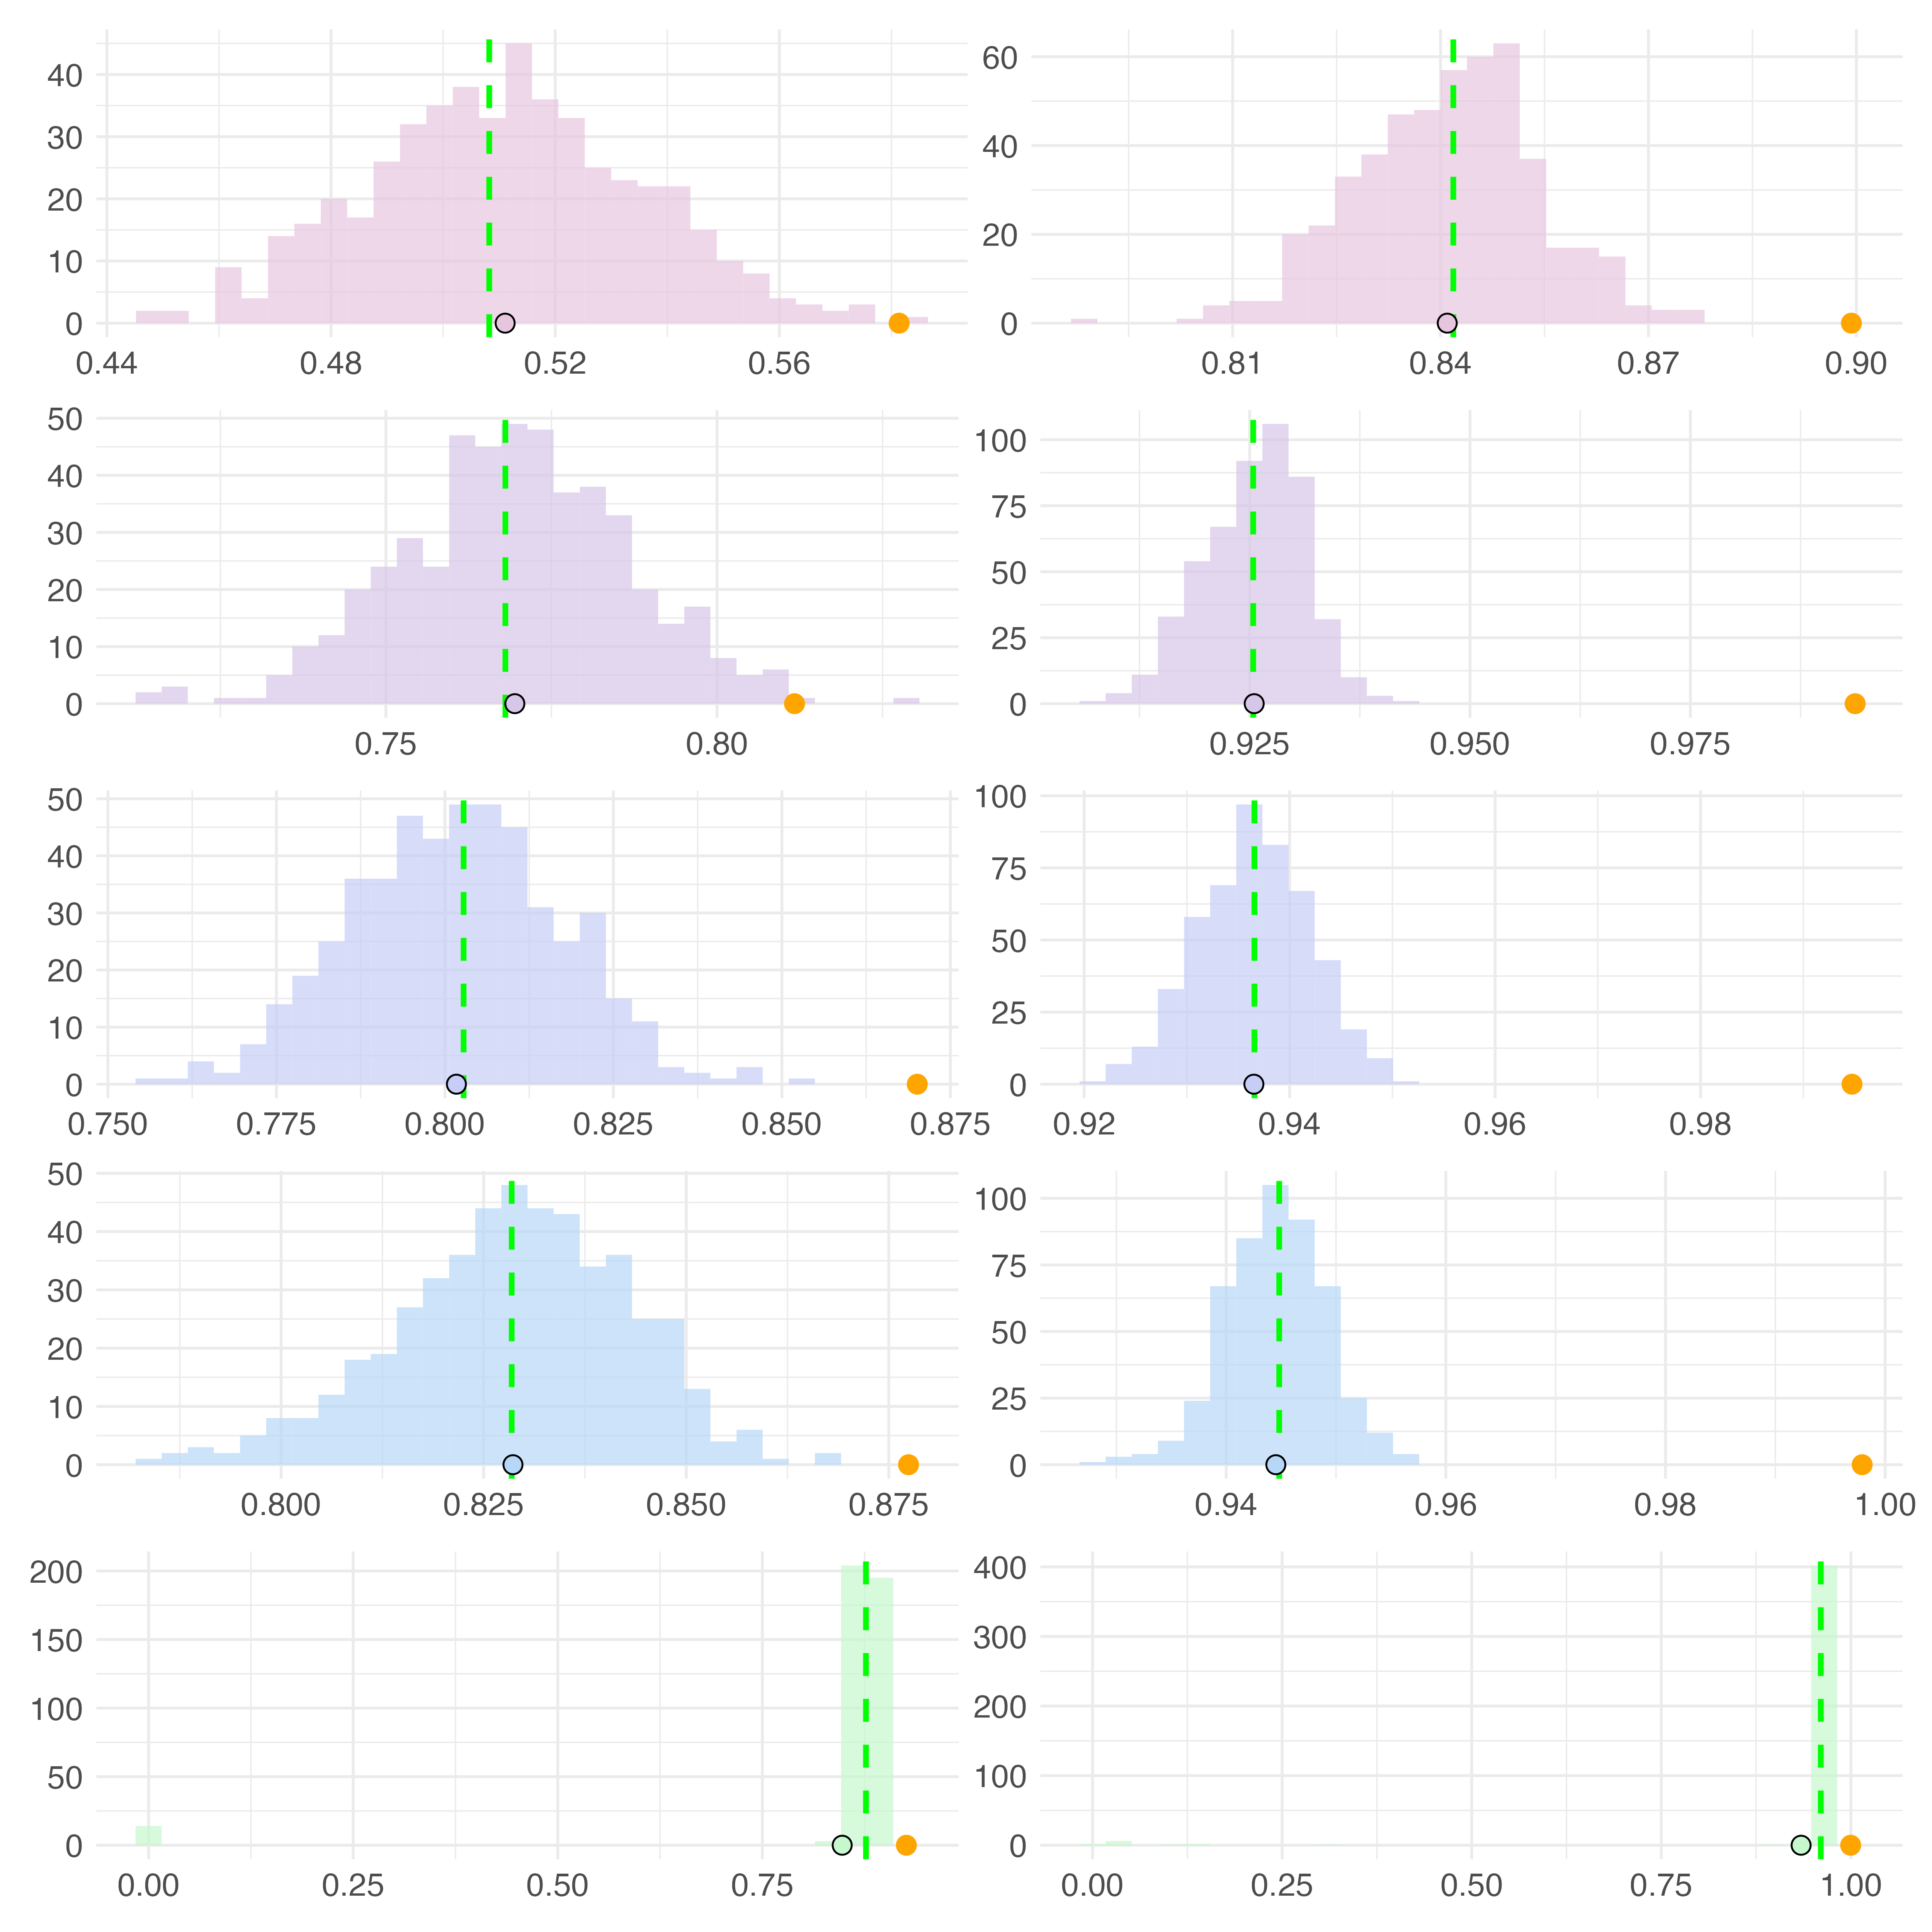
\includegraphics[width=1\linewidth]{Figures/Simulation study/R2_combined_poisson.png}
  \caption[Marginal and conditional $R^2$ in Poisson GLMM]{Histograms with the posterior modes of the estimated marginal and conditional $R^2$ from the BVI method for the Poisson regression for the different correlation levels $\rho$. The modes are calculated by the Bayesian Variable Importance method from the $N_{\text{sim}}=500$ models fit in the simulation study. The expected values are displayed as vertical green lines, and can be found in \Cref{table:r2values}, while the orange dot denotes the estimate from the \texttt{rptR} package. The mean value of the $R^2$ modes for all simulations is marked with a circle at the bottom of each histogram.}
  \label{fig:r2_combined_poisson}
\end{figure}
\section{Case study with \texttt{rptR} package}
% \begin{figure}[H]
%     \centering
%       \includegraphics[width=0.7\linewidth]{Figures/Stoffel Comparison/Heritability_colour_Binomial.png}
%       \caption{Heritability of colour of male beetles from Stoffel}
%       \label{fig:heritability_colour_Binomial}
%   \end{figure}
%   \begin{figure}[H]\ContinuedFloat
%     \centering
%     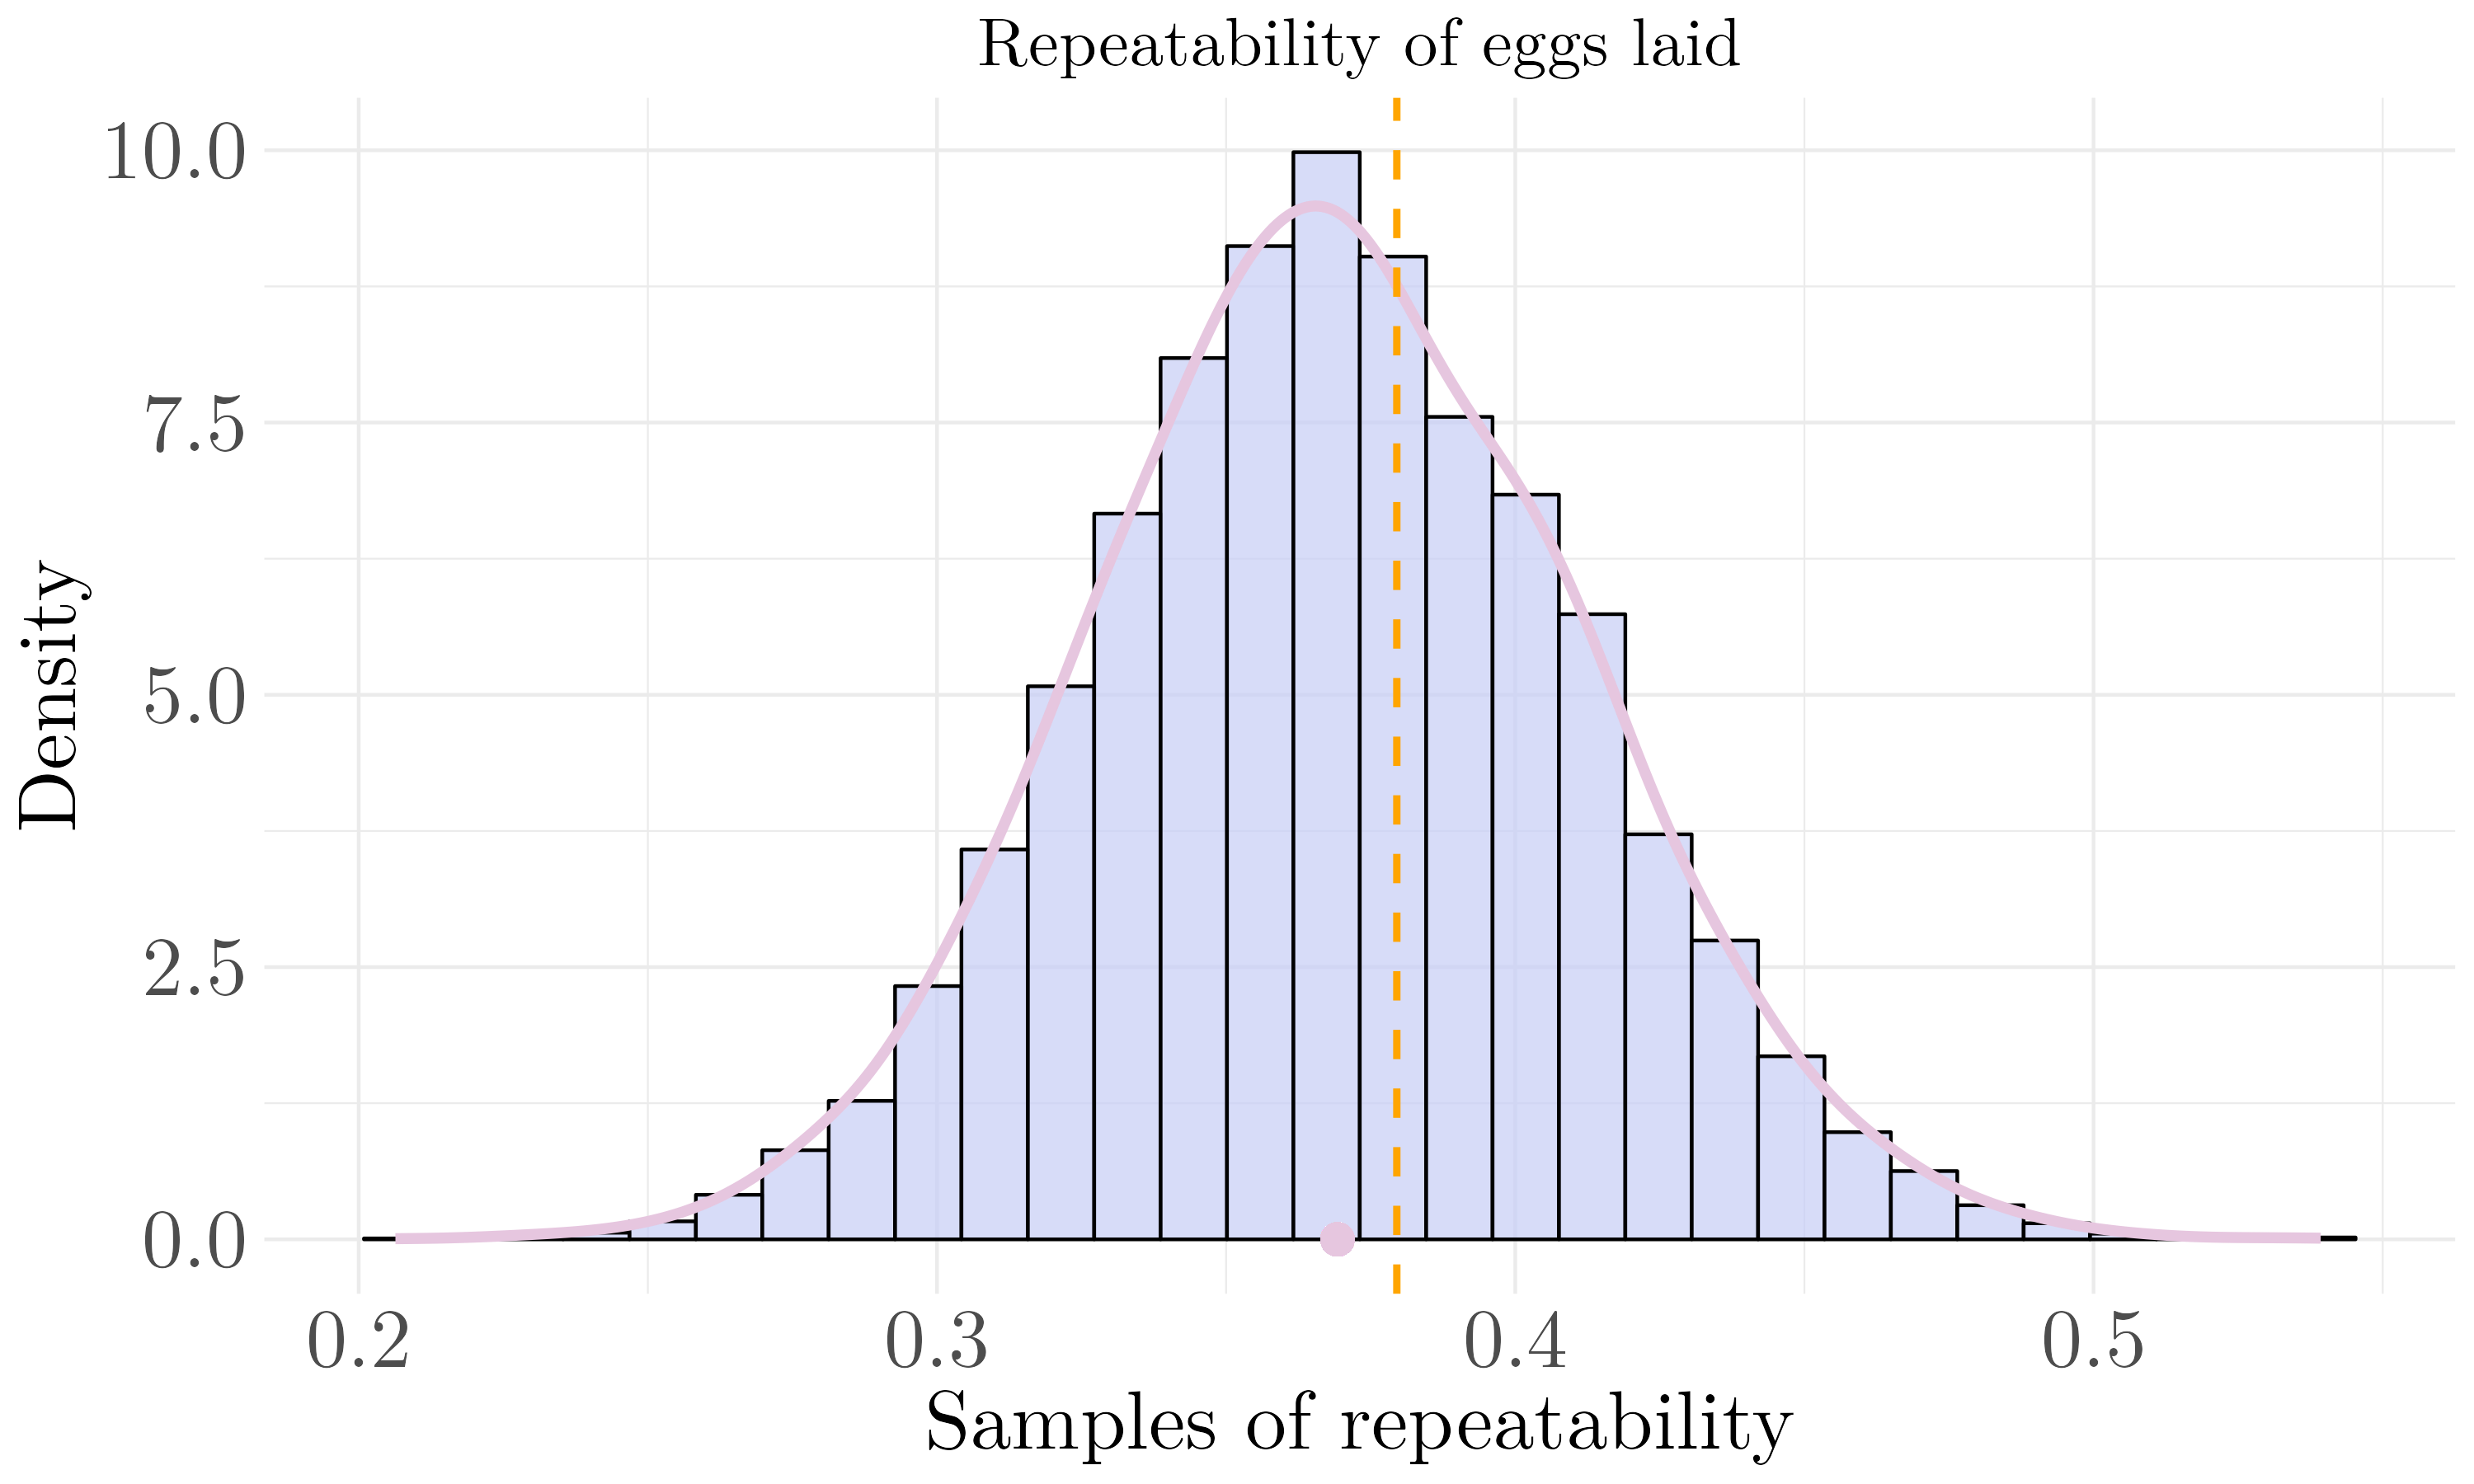
\includegraphics[width=0.7\linewidth]{Figures/Stoffel Comparison/Heritability_egg_poisson.png}
%     \caption{Heritability of eggs laid by female beetles from Stoffel}
%       \label{fig:heritability_egg_poisson}
%   \end{figure}
To further assess our method, a comparison to the vignette for the \texttt{rptR} was made. The package described in this vignette estimates the repeatability of phenotypic traits, which for some definitions coincide with heritability and therefore can be seen as a special case of variable importance. Thus, we were able to apply the Bayesian Variable Importance method and compare the results. No expected results were available, and so we can only compare our method to the results made by the authors of the vignette. It should however be noted, that the \texttt{rptR} package returns the marginal $R^2$ as the only measure of importance for the fixed effects, whereas our method directly decomposes this value and assigns a share to each fixed effect. To obtain uncertainty estimates in the likelihood framework, Stoffel, Nakagawa and Schielzeth have built in bootstrap functionality. This is used in our comparison, to evaluate computational complexity and confidence intervals.
\\
\\
The repeatability of the color of male beetles is modelled by a binomial GLMM with binary outcome and logit-link. We use the same formulation as in the model \texttt{rep11} from the vignette \citep{Stoffel2017rptR}, with the parameter \texttt{adjusted=FALSE}. We see that the sampled posterior distribution of repeatability (\Cref{fig:heritability_colour_Binomial}) from the Bayesian Variable Importance method is centered around a mean of $0.193$, which is very similar to the estimate by Stoffel which is $0.196$. The obtained distribution appears unimodal, with the mode and mean aligning closely. Perhaps a slightly longer tail on the right side can be observed. From $10^3$ bootstrap samples, the \texttt{rptR} estimates a $95\%$ confidence interval of $[0.051, 0.338]$, which is a bit larger than our estimated $95$th percentile of $[0.114, 0.280]$. In terms of computation time, the Bayesian Variable Importance method used $6$ seconds to obtain the model fit and $10^4$ samples, whereas the \texttt{rptR} package used $66$ seconds to obtain the model fit and the same number of bootstrap samples.
\begin{figure}[H]
  \centering
  % First row
  \includegraphics[width=1\linewidth]{Figures/Stoffel Comparison/Heritability_colour_Binomial.png}
  \caption[Estimated repeatability of color in male beetles]{Histogram with values sampled from the posterior distribution of repeatability for the color of male beetles from the BVI method, with the mean of the samples denoted by a pink circle. The estimate from the \texttt{rptR} package marked as a dashed line with orange color.}
  \label{fig:heritability_colour_Binomial}
\end{figure}
% We see that the approximated distribution from the BVI method is centered a bit to the right of the point estimate from \texttt{rptR}. The stochasticity of the BVI method makes it so that the distributions return will vary based on what seed was made to generate the results. Therefore, we expect to see a difference between the centering of the distribution and point estimates. 
\noindent To estimate the repeatability of the number of eggs laid by female beetles, we use a Poisson GLMM with log-link. The model used in our method corresponds to \texttt{rep9}, but as is described in the vignette after fitting \texttt{rep9}, we set the option \texttt{expect="latent"} so that the method calculates the distributional variance as in \Cref{table:1}. This corresponds to the recommendations of \citet{nakagawa2017} as previously mentioned. Likewise, this model is estimated from the \texttt{rptR} package with \texttt{adjusted=FALSE}. From the plotted samples of posterior repeatability of eggs laid (\Cref{fig:heritability_eggs_poisson}), we see a very similar distribution as that of the binomial color model. The distribution is symmetric and centered around a mean of $0.369$. Further, the estimate from the \texttt{rptR} model is $0.380$ with a confidence interval of $[0.131, 0.542]$, compared to our $95$th percentile of $[0.288, 0.453]$. The $10^3$ bootstrap samples and model fit for the \texttt{rptR} package took $2$ minutes and $13$ seconds, whereas the BVI method used $8$ seconds to obtain the model fit and $10^4$ samples.
% \begin{figure}[H]
%   \centering
%   \begin{subfloat}{0.49\linewidth}
%       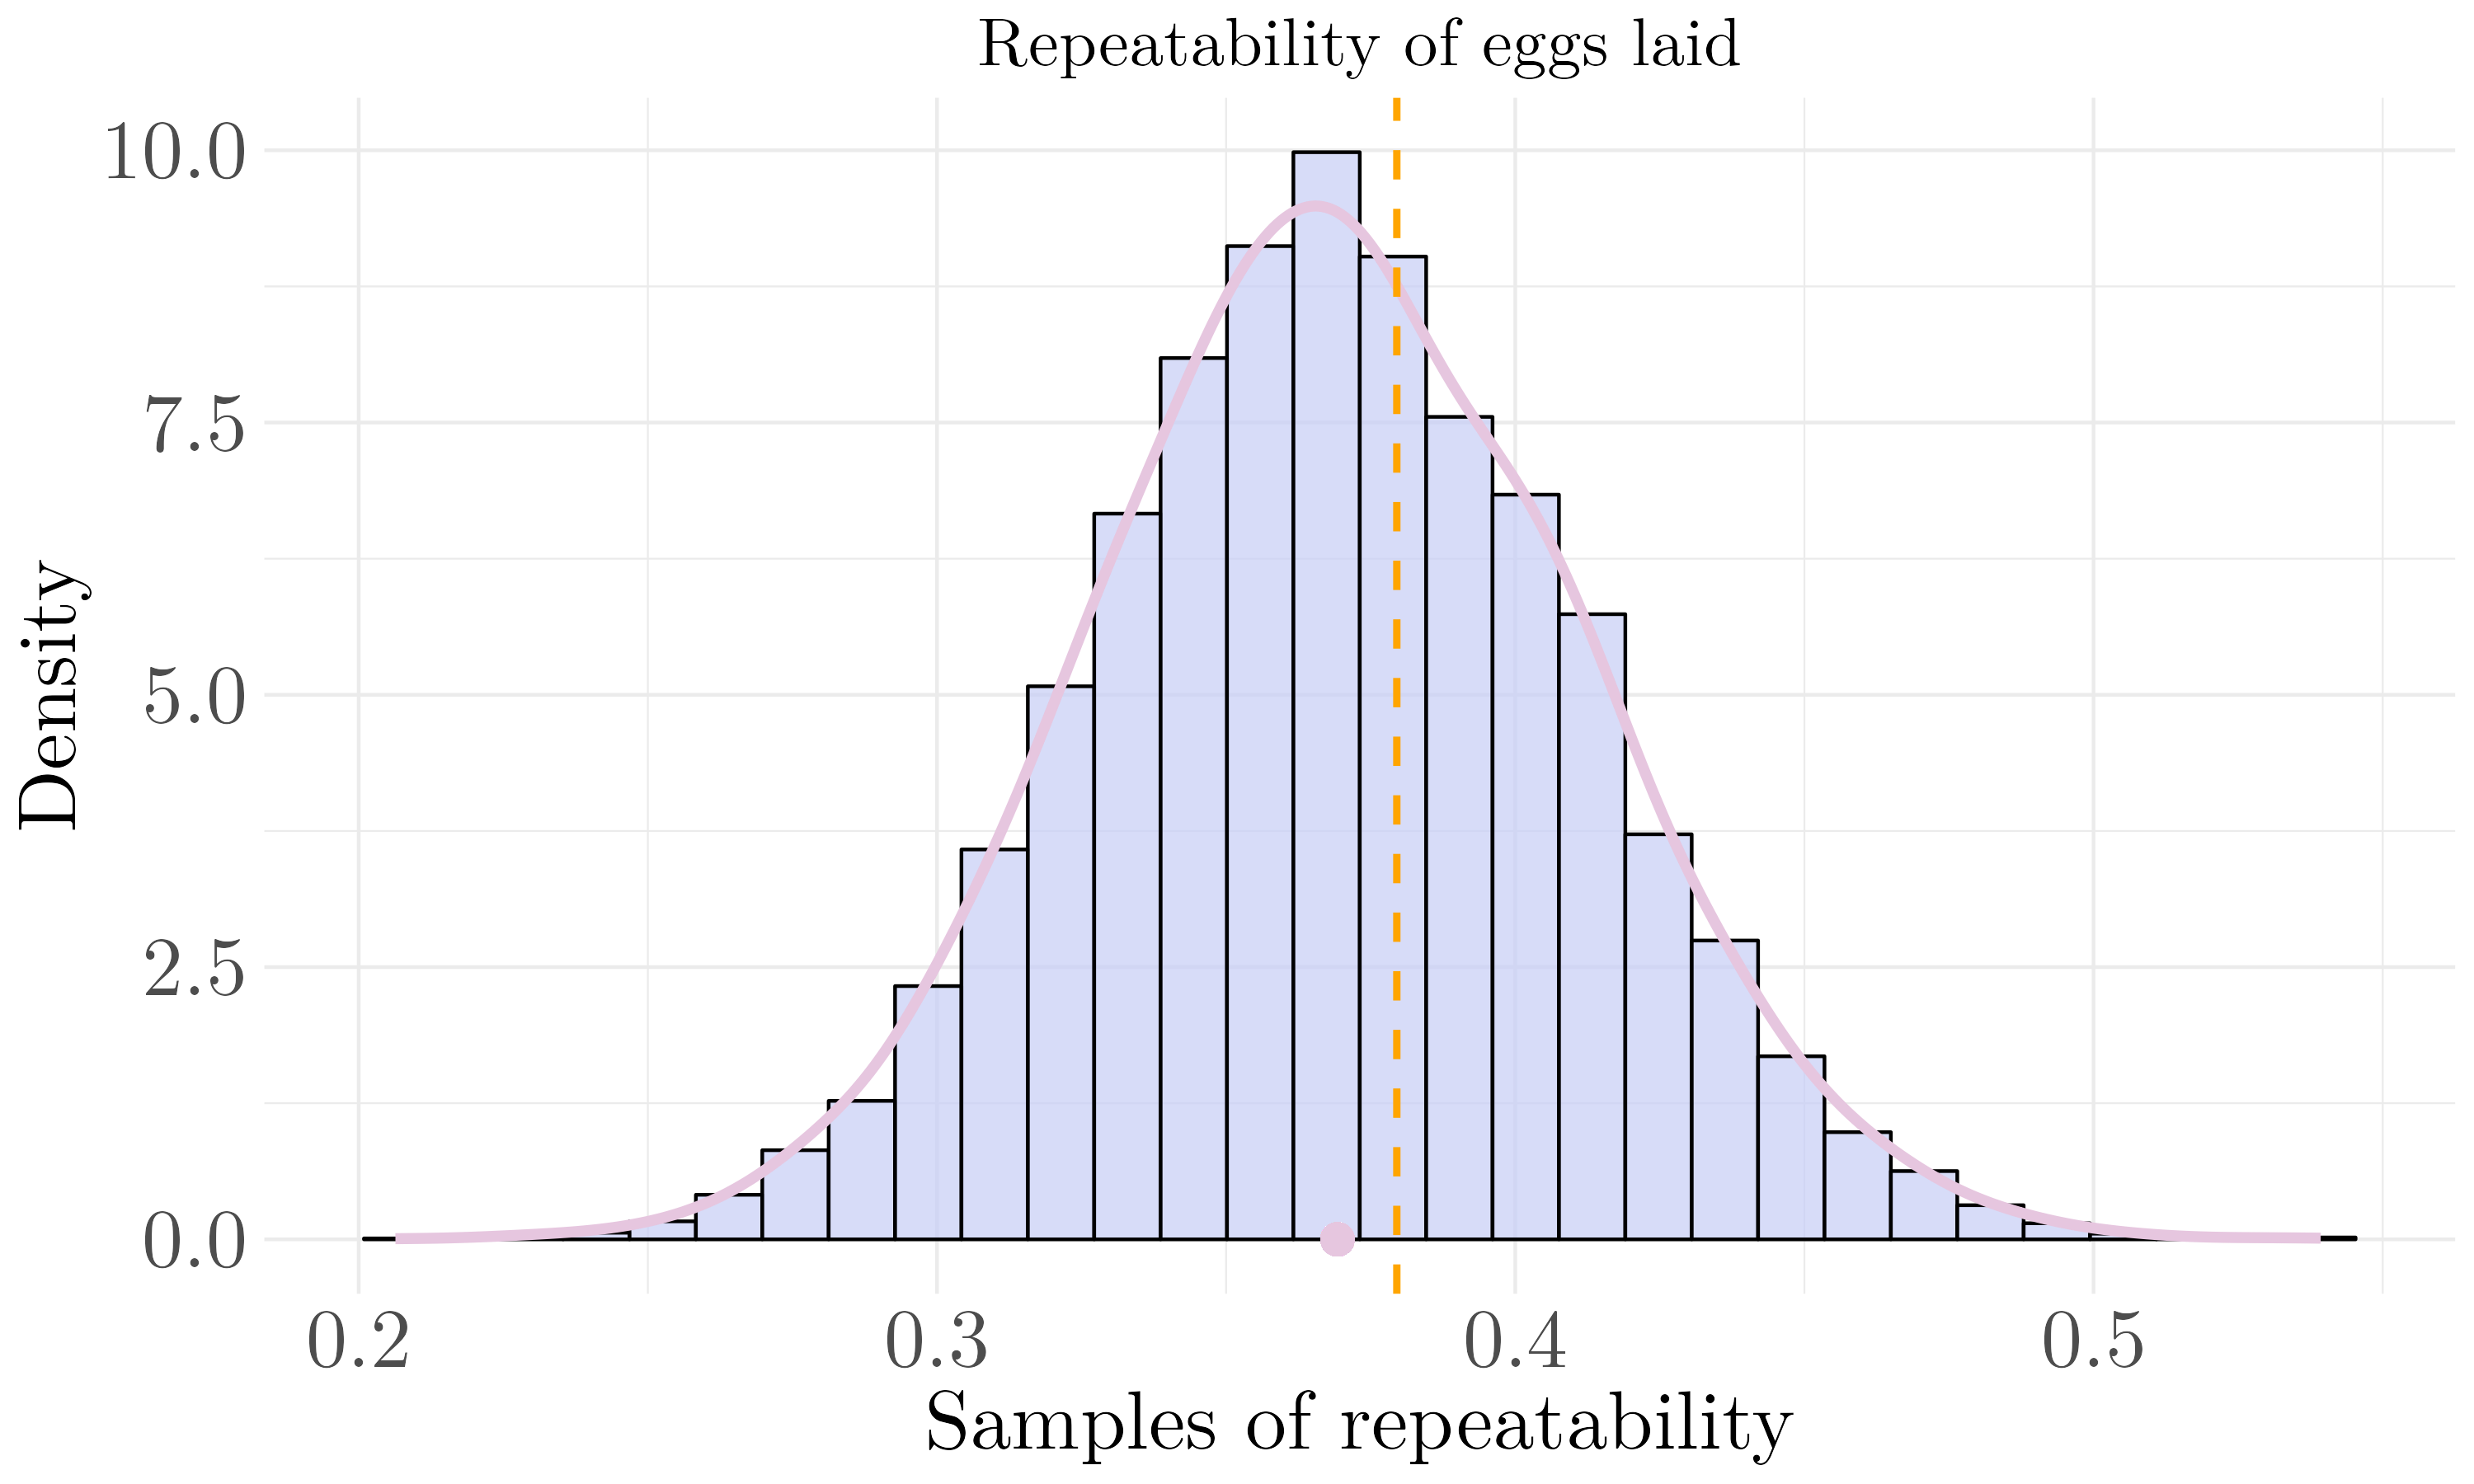
\includegraphics[width=\linewidth]{Figures/Stoffel Comparison/Heritability_egg_poisson.png}
%       \caption{Heritability of eggs laid by female beetles from BVI}
%       \label{fig:heritability_egg_poisson}
%   \end{subfloat}
%   \hfill
%   \begin{subfloat}{0.49\linewidth}
%       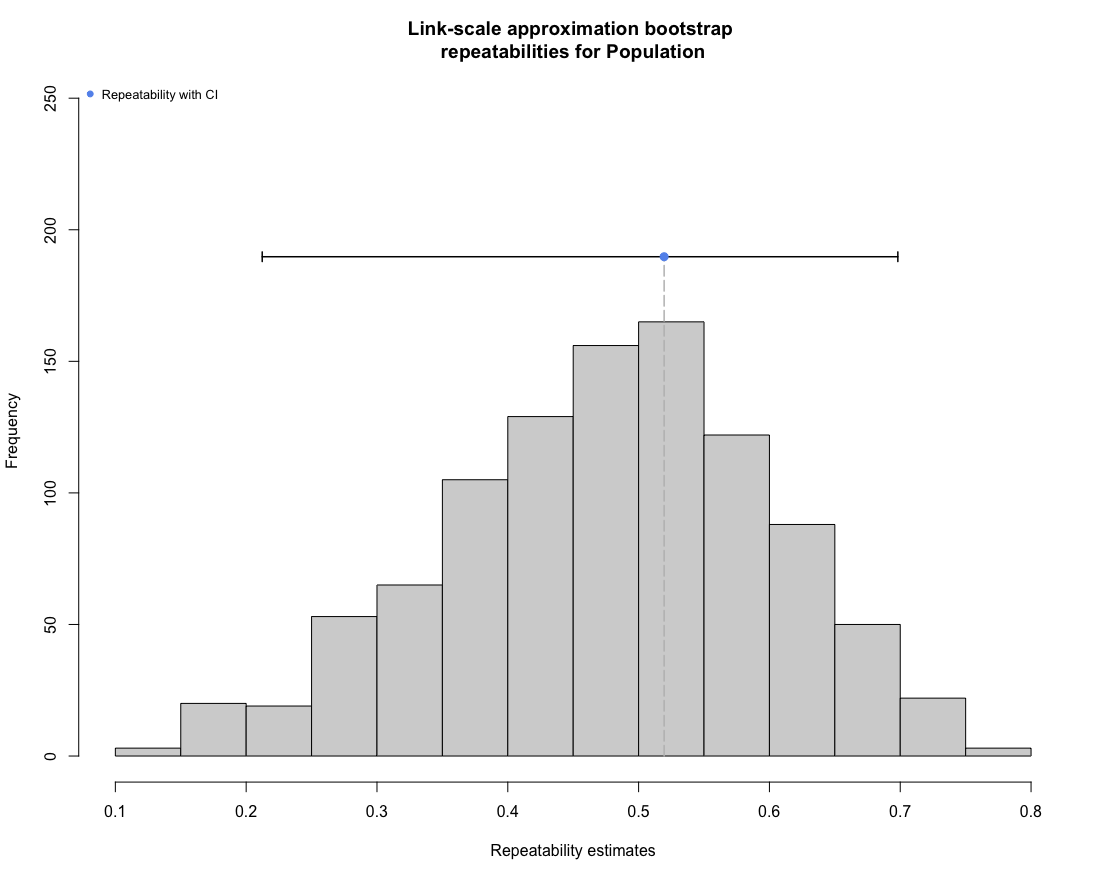
\includegraphics[width=\linewidth]{Figures/Stoffel Comparison/Heritability_egg_poisson_Stoffel.png}
%       \caption{Comparison of heritability of eggs from Stoffel}
%       \label{fig:comparison_heritability_egg}
%   \end{subfloat}
%   \caption{Heritability of eggs in female beetles and comparison}
% \end{figure}
\begin{figure}[H]
  \centering
  % First row
  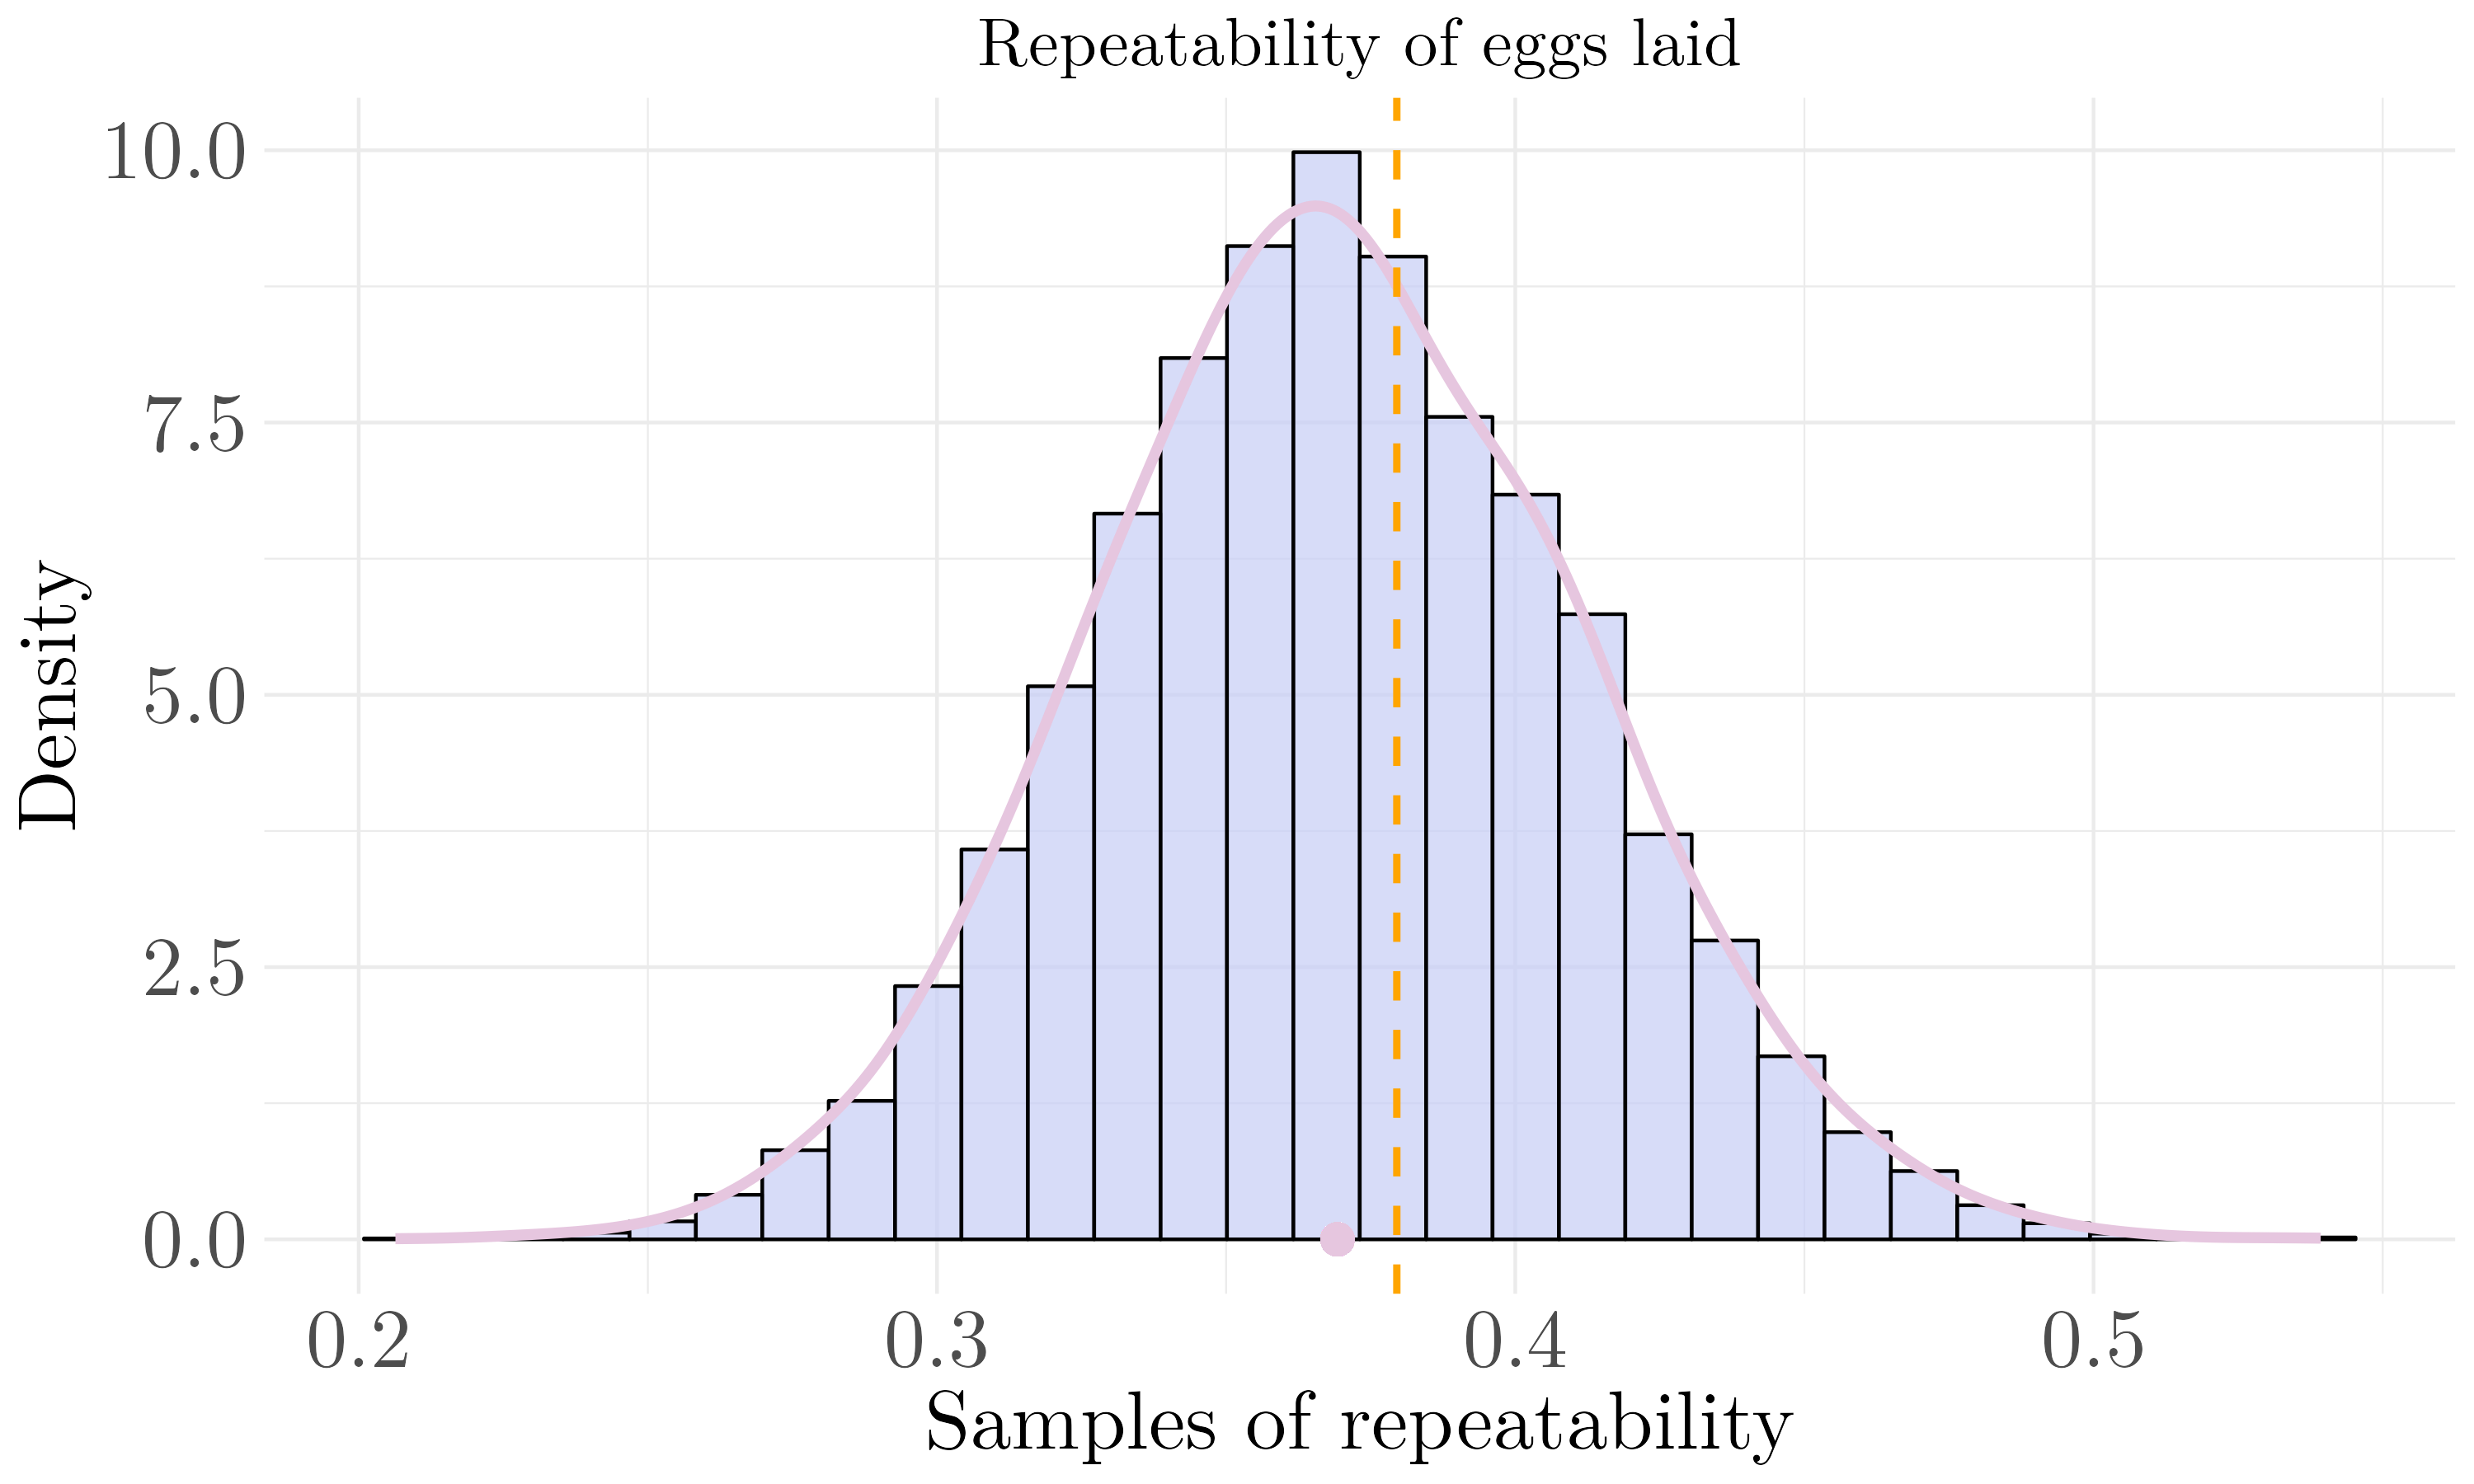
\includegraphics[width=1\linewidth]{Figures/Stoffel Comparison/Heritability_egg_poisson.png}
  \caption[Estimated repeatability of eggs laid by female beetles]{Histogram with values sampled from the posterior distribution of repeatability for eggs laid by female beetles from BVI method, with the mean of the samples denoted by a pink circle. The estimate from the \texttt{rptR} package marked as a dashed line with orange color.}
  \label{fig:heritability_eggs_poisson}
\end{figure}
\noindent Importantly, note that the estimates from the BVI method will vary each time a model is fit, as it is stochastic. In this comparison, we only fit a single Bayesian GLMM with the BVI method. Therefore, it could be that another fit from the BVI method might align closer with the results of Stoffel and Nakagawa, but it could also be further off. 

% \section{Comparing the BVI method with \texorpdfstring{$R^2$}{Lg}-induced Dirichlet decomposition priors and Generalized Decomposition Priors on \texorpdfstring{$R^2$}{Lg}}
\section{Comparing the BVI method with Dirichlet and Generalized Decomposition Priors on \texorpdfstring{$R^2$}{Lg}}
To explore other possible relative variable importance tools in the Bayesian framework, we have discussed R2D2 and GDR2 priors in \Cref{sec:R2D2} and \Cref{sec:r2d2method}. We now present the results of applying the R2D2 and GDR2 priors to a linear regression, and see how they can be interpreted as relative importance measures. The results are compared to the sampled posterior relative importances computed by the BVI method and the LMG method serves as a robust benchmark for all methods. Please note once again that the R2D2 and GDR2 priors are originally developed for prediction models, and that the results presented here are based on our interpretation of how the R2D2 and GDR2 priors can be used for relative importance. The theoretically expected importances for uncorrelated covariates are found in \eqref{eq:RI_R2D2} and the theoretical $R^2$ for all correlation levels are found in \Cref{table:r2values_r2d2}. 
\begin{figure}[H]%\ContinuedFloat
  \centering
  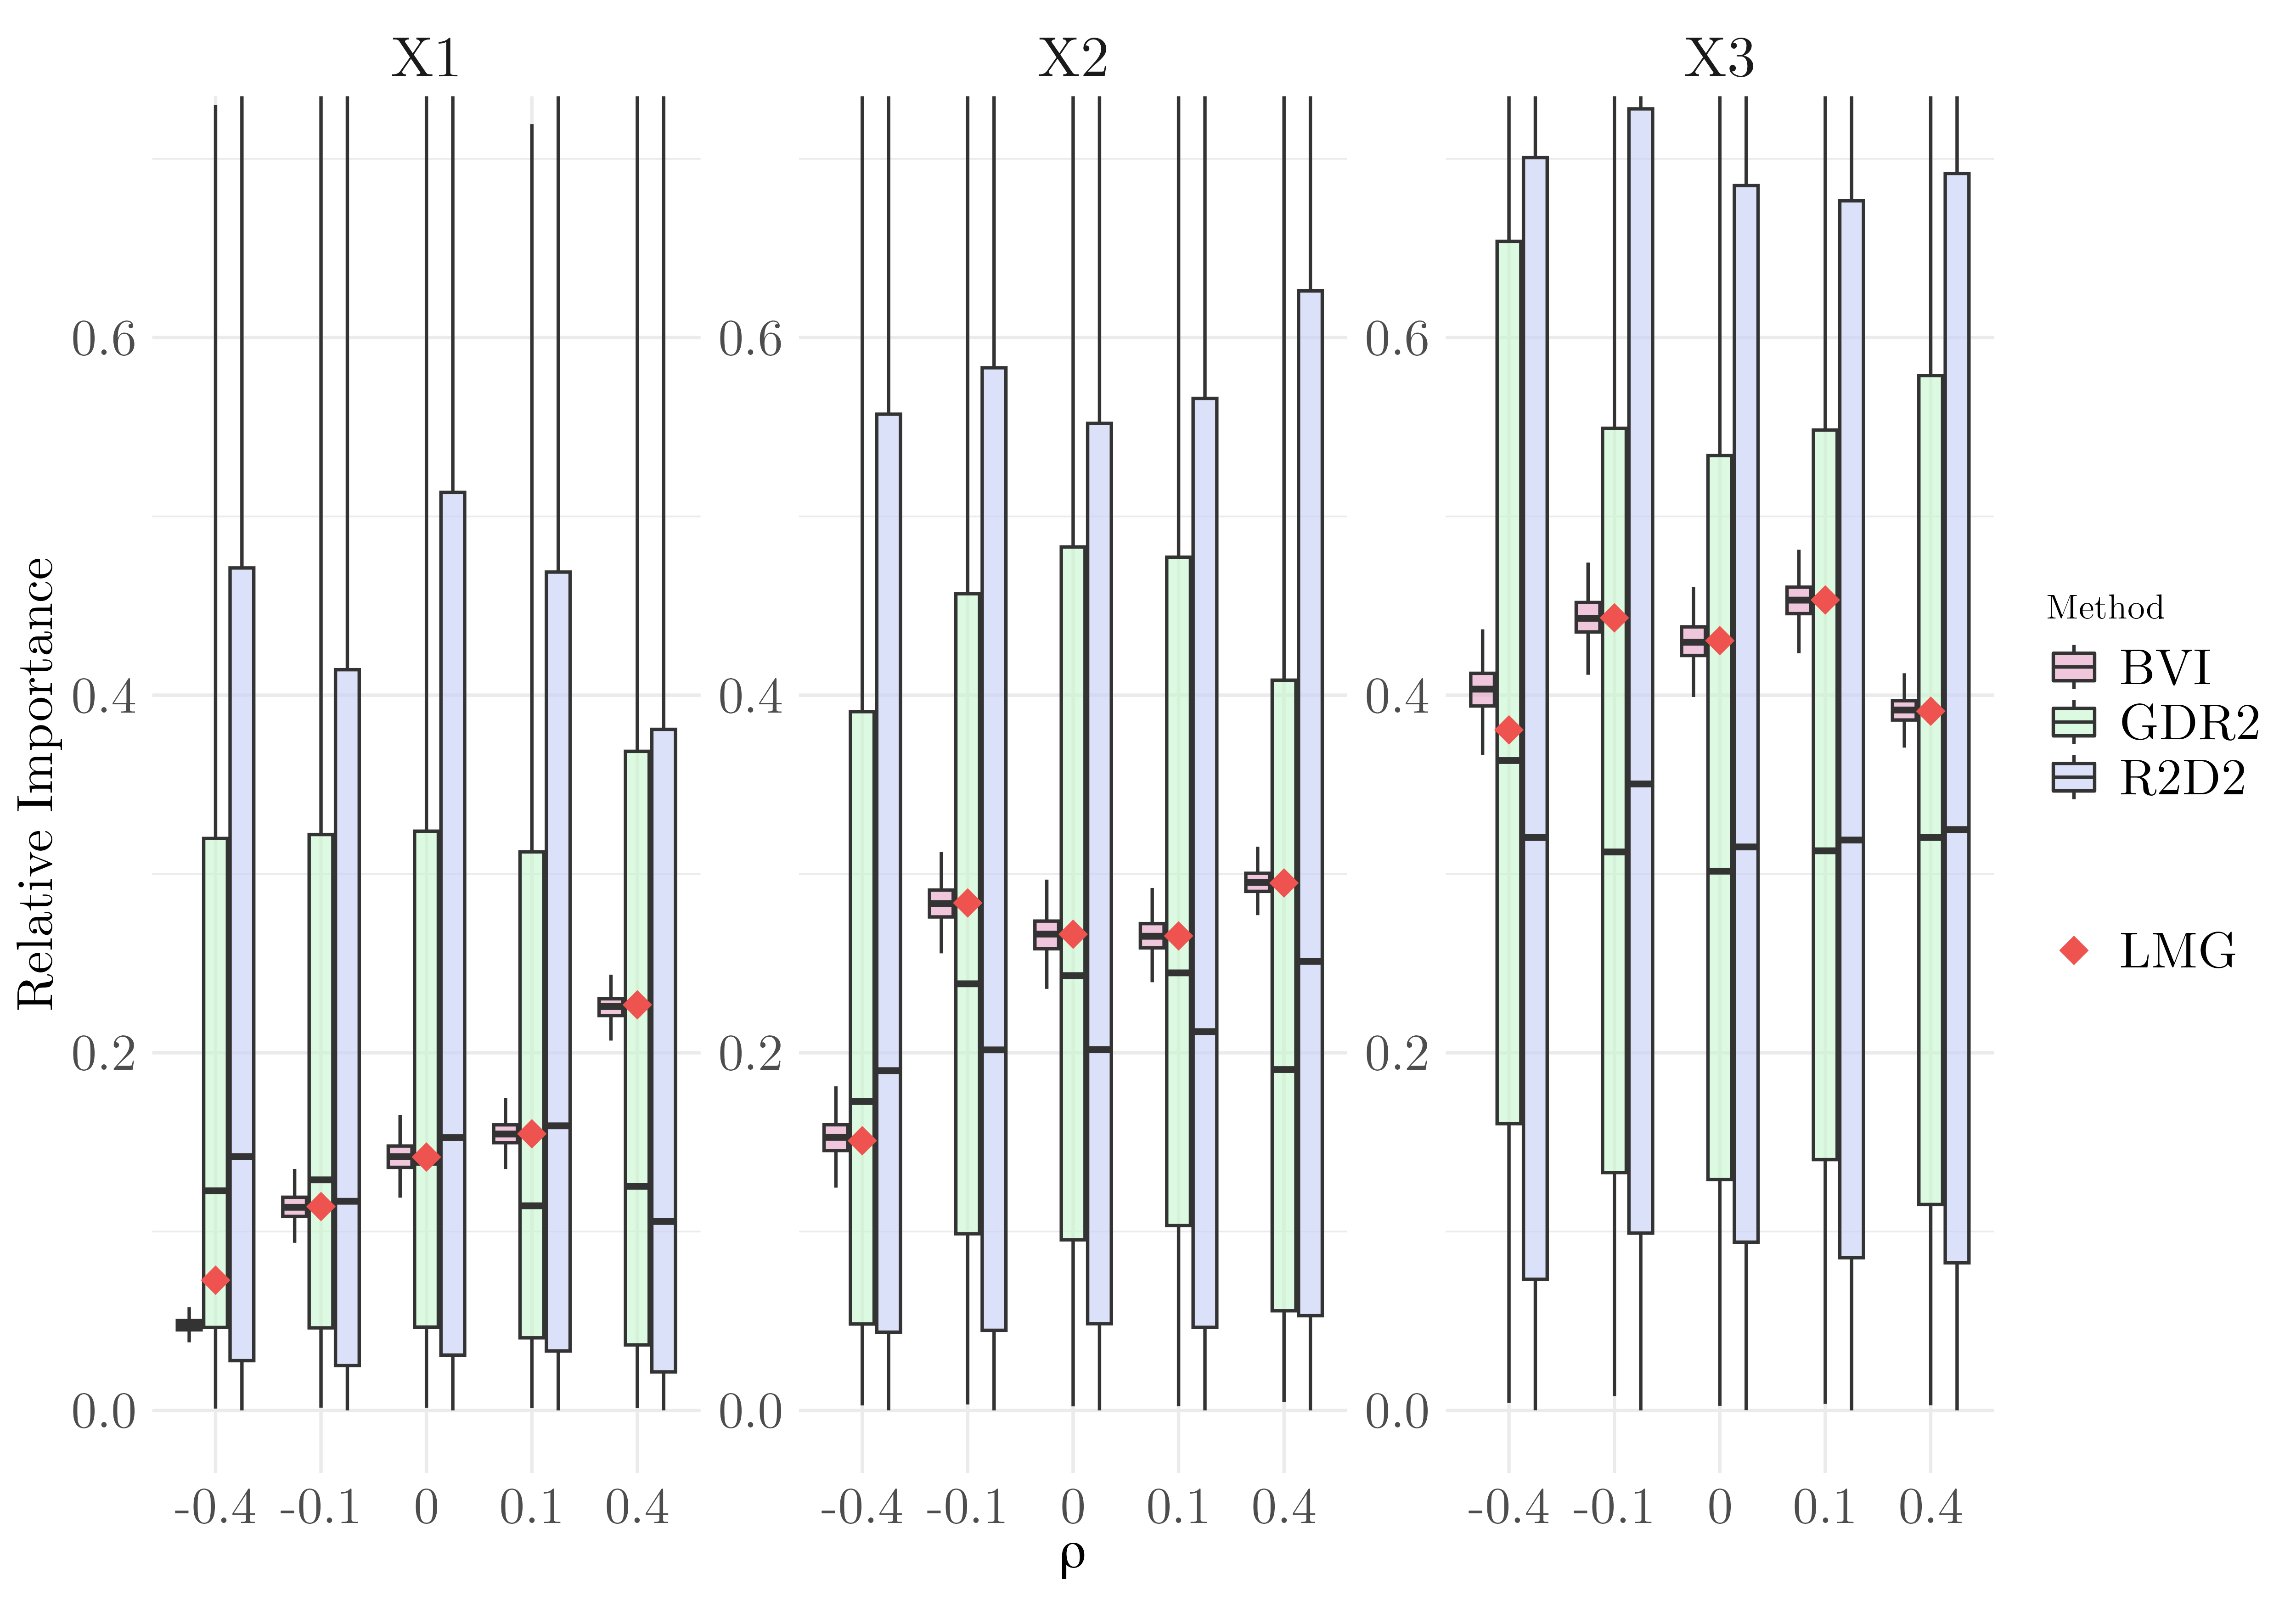
\includegraphics[width=1\linewidth]{Figures/R2D2_BVI_Comparison/R2D2_BVI_boxplot.png}
  \caption[Comparison of the relative importance from the BVI method and the shrinkage prior methods]{Box plots of the relative importance distributions for $X_1$, $X_2$ and $X_3$ for varying correlation levels by the R2D2, GDR2 and BVI methods. The correlation levels $\rho$ are denoted along the x-axis, and the red diamond represents the relative variable importance calculated from the LMG method.}
  \label{fig:r2d2_importance}
\end{figure}
\noindent The first thing one notices from the posterior relative importance distributions (\Cref{fig:r2d2_importance}), is that the spread from the R2D2 method is larger than the spread of the GDR2 method, which again is significantly larger than the spread of the BVI method. In the box plots, the $25$th and $75$th quantiles define the interval of each box. The mean values of the relative importance distributions for the R2D2 and GDR2 methods do not seem to follow any pattern at all for varying correlation. They are more similar across correlation levels for all covariates and do not adjust for correlation as the benchmark LMG method and the BVI method does. Although it is hard to find patterns, and the R2D2 and GDR methods give very flexible results, they clearly grasp the larger aspects, with $X_3$ estimated to be the covariate with the largest variance contribution, followed by $X_2$, and lastly $X_1$. The BVI method is in close agreement with the LMG method, except for some small deviations for $X_1$ and $X_3$ when $\rho=-0.4$. Overall, the BVI and LMG methods follow the same pattern for varying correlation, as we expect and have previously discussed.
\begin{figure}[H]%\ContinuedFloat
  \centering
  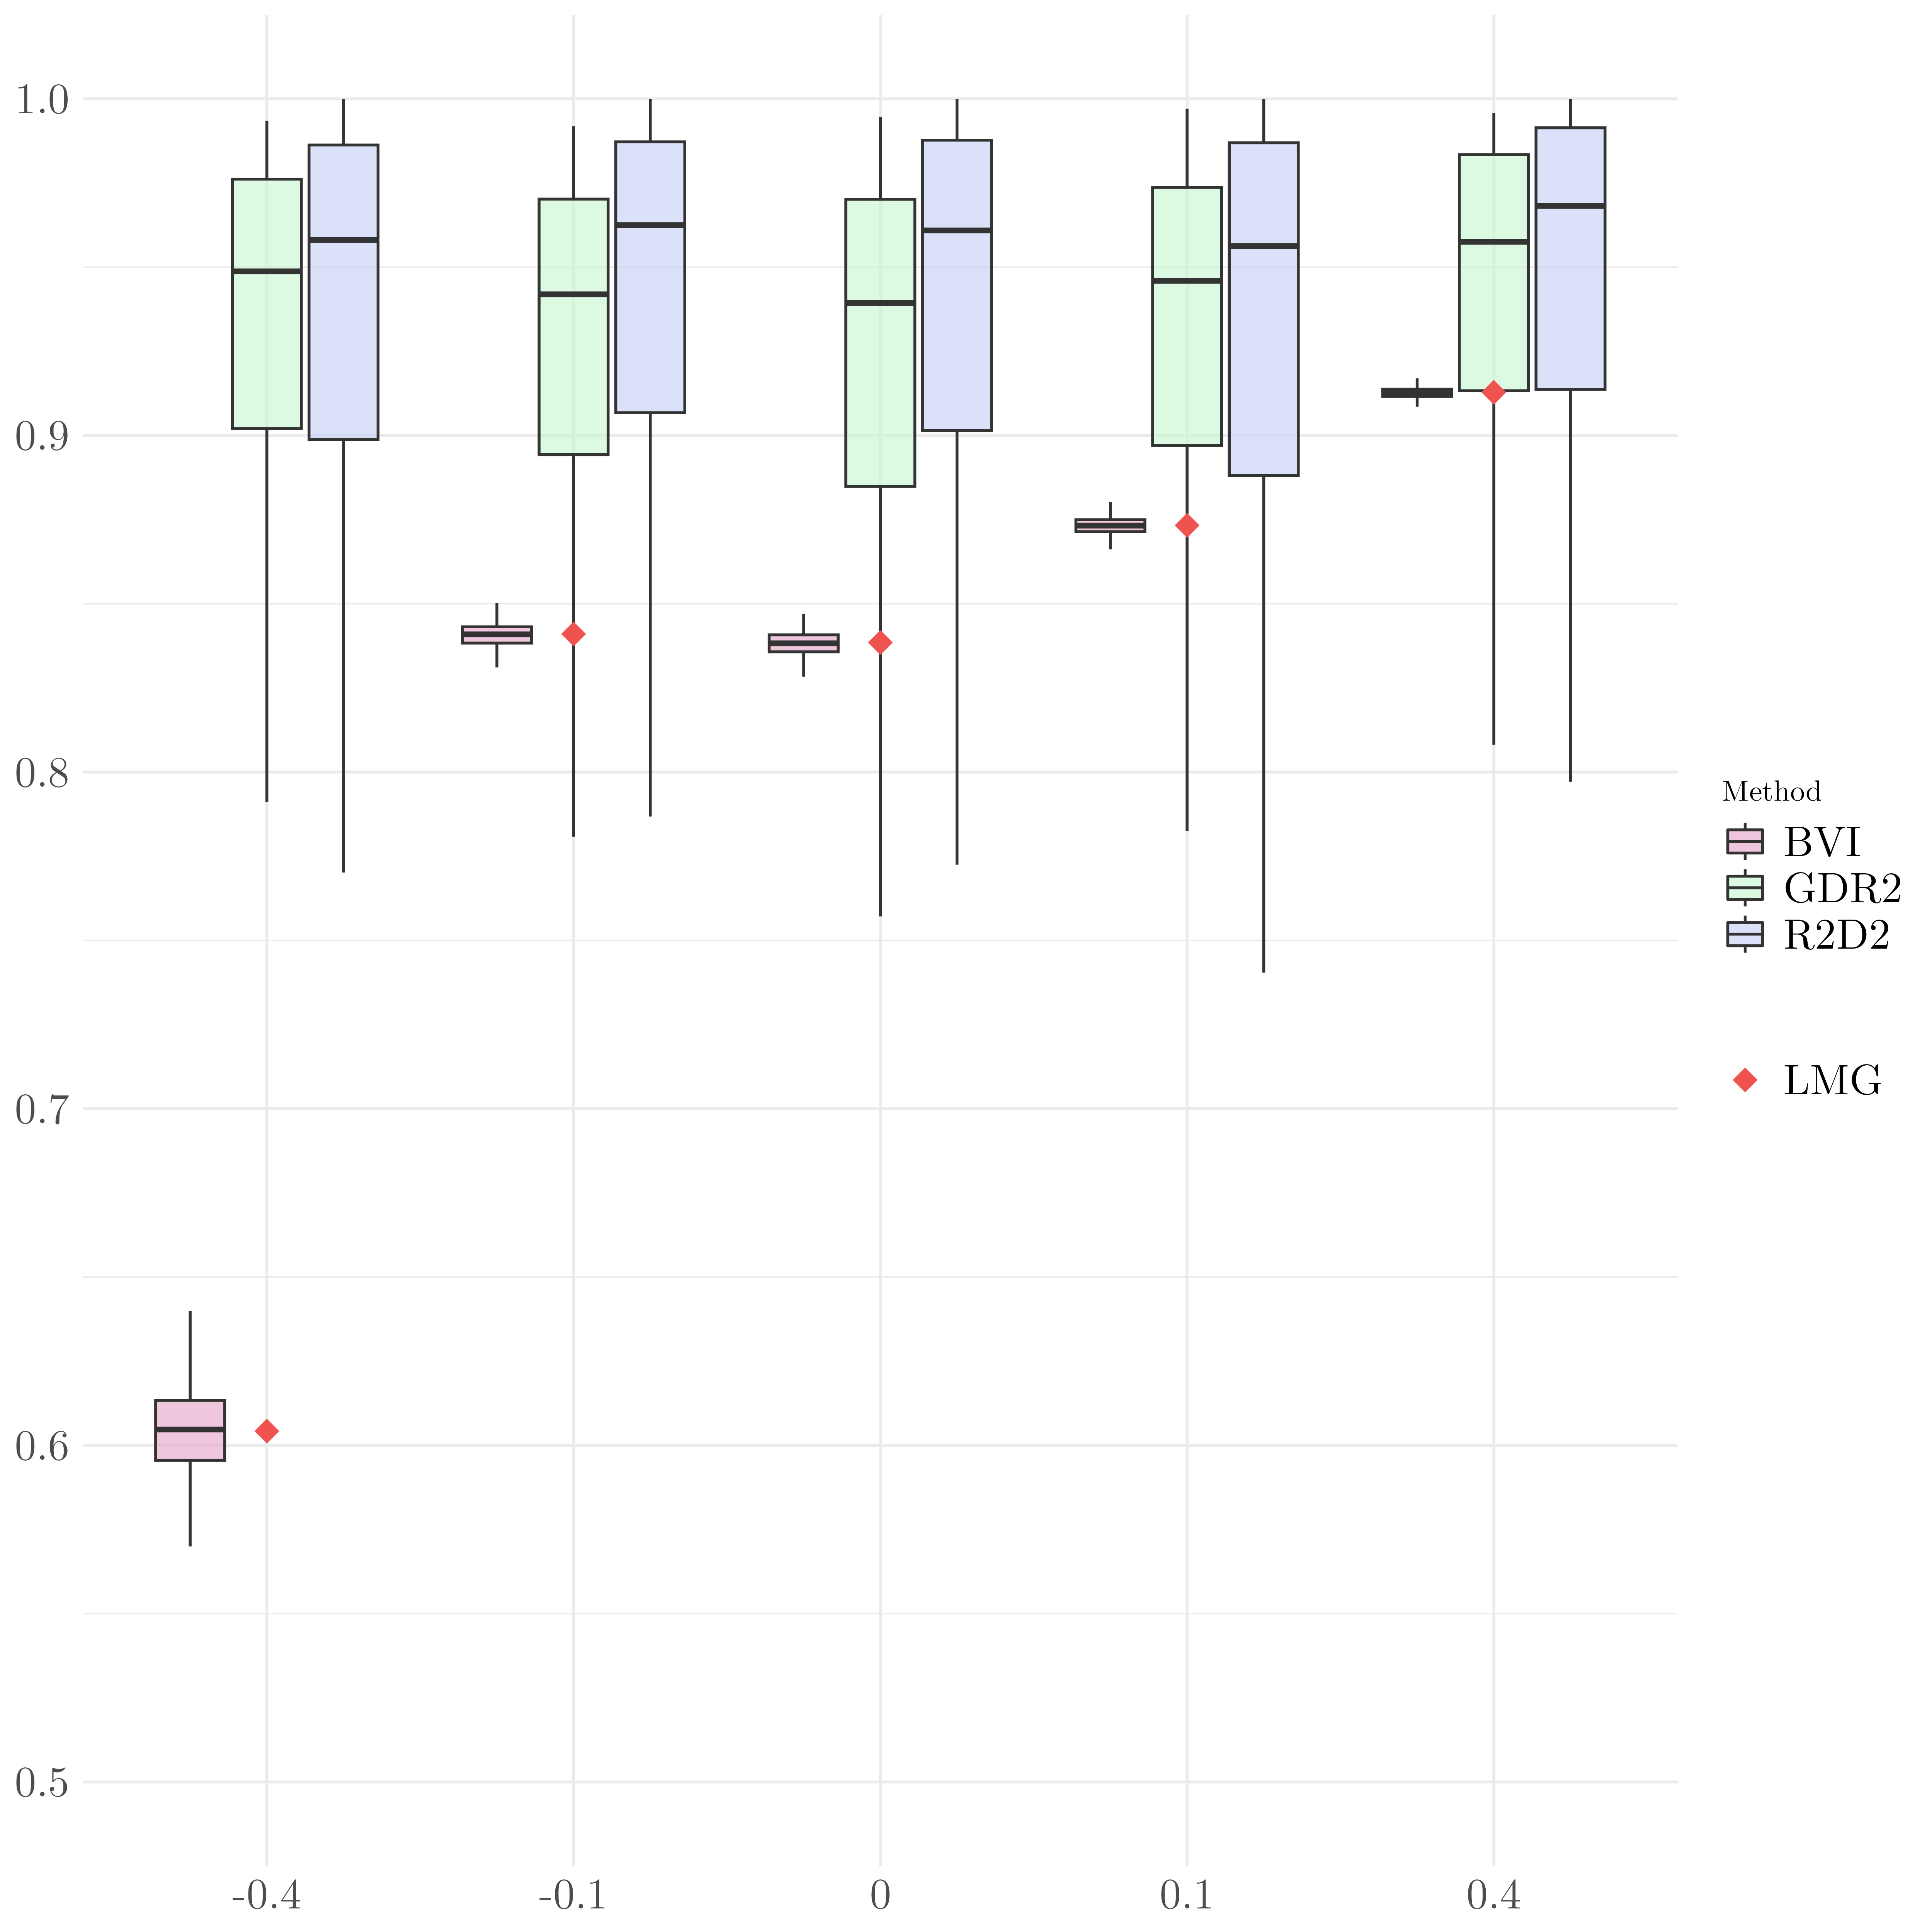
\includegraphics[width=1\linewidth]{Figures/R2D2_BVI_Comparison/R2D2_BVI_R2_plot.png}
  \caption[Comparison of the marginal $R^2$ from the BVI method and the shrinkage prior methods]{Box plots of the estimated $R^2$ distributions for varying correlation levels $\rho$ for the R2D2, GDR2 and BVI methods. The correlation levels $\rho$ are denoted along the x-axis, and the red diamond represents the marginal $R^2$ calculated from the LMG method.}
  \label{fig:r2d2_r2}
\end{figure}
\noindent The estimated posterior marginal $R^2$ distributions with the R2D2 and GDR2 priors (\Cref{fig:r2d2_r2}) are uniform across the correlation levels, and significantly larger than both the estimates of the BVI and LMG methods. For the $R^2$, the spread of the R2D2 and GDR2 methods are quite similar, with both being considerably larger than that of the BVI method. Overall, the R2D2 and GDR2 estimates a substantially larger $R^2$ than the BVI and LMG methods, and the means deviate significantly from the expected values. The BVI method is consistent with the LMG method, and they both follow the expected pattern of the $R^2$ when the correlation levels vary. For the expected $R^2$, the BVI and LMG methods seem to align closely with the expectation, with a small deviation for both methods when $\rho=0$.
\\
\\
As the R2D2 and GDR2 methods are not specifically relative variable importance measures, one should also interpret the results with this in mind. The development of the R2D2 and GDR2 priors have been done to produce robust predictions for high dimensional linear regression models, and the results presented here are therefore not an evaluation of the R2D2 and GDR2 priors as relative importance measures. Moreover, the interpretation made to obtain these results was made by the author, and the results should be taken with caution. The main motivation behind this comparison was to explore other possible relative importance measures in the Bayesian framework, as this is a small field with few available methods. 





\cleardoublepage

%\chapter{Simulation study}
%\input{Chapters/05Simulation study}
%\cleardoublepage

%If we get this far
%\chapter{Animal model for sparrows}
%Linear model
Linear mixed model
GLMMs
proof of Bayesian Importance in expectation?
R^2
Bayesian framework
Animal model as (generalized) linear mixed model
GLMM 
INLA framework
Animal Model as a GMRF
Parameter estimation




Results:
Fit gaussian traits with INLA and MCMCglmm and compare. First do a simulation, then do animal model? or go straight to animal model?


Fit binary traits with INLA and MCMCglmm. Additive overdispersion is set to 1 and distribution specific variance is set to pi^2/3.
Is the additive overdispersion the same as the IDC variable?


Package for computing the posterior distribution of the parameters and heritability

%\cleardoublepage


\chapter{Discussion \& Further work}
\label{ch:discussion}
The main objectives of this thesis were to develop a general variable importance method applicable to a wide range of GLMMs, allowing complex covariance structures in the random effects, and to provide interpretable and trustworthy results. In addition, the method should be easily accessible for researchers across disciplines, and be computationally feasible in most applications. Our attempt to reach these objectives has culminated in the Bayesian Variable Importance (BVI) method, which is a novel framework for estimating relative variable importance in generalized linear mixed models. The work presented in this thesis is motivated by the increased inference possible in the Bayesian framework and partially builds on the author's previous work in \citet{Arnstad:Relative_variable_importance_in_Bayesian_linear_mixed_models:2024} and that of \citet{matre}.
\\
\\
\subsection*{Summary of contributions} 
The development of the BVI method involved utilizing the relative weights method \citep{johnson_relative_weights} to project the fixed covariates into an orthogonal space. The projection, or approximation, of these covariates is used to fit the model, before a back-transformation is applied to relate the estimated results back to the original covariate space. To obtain inference on the Bayesian GLMMs, we translated frequentist concepts, such as the $R^2$ measure, to fit in the Bayesian framework. This translation has been inspired by the work of \citet{gelman2017rsquared}, but is the result of the author's own work. Once the methodology was developed, we revisited a Gaussian simulation study from \citet{Arnstad:Relative_variable_importance_in_Bayesian_linear_mixed_models:2024}. This simulation study indicated that the BVI method was sound for the LMMs, and so it was applied to a real world dataset. The dataset, gathered from house sparrows on the Helgeland coast, Norway, was used to investigate the heritability properties of the sparrow population. We found that the BVI method was in close agreement with other heritability studies, which was reassuring. In addition to calculating heritability, we demonstrated how the BVI method allows for a more in-depth analysis by sampling the posterior relative importance distributions of all covariates used in the model. Moving from the LMMs to the GLMMs, we conducted a simulation study for the binomial and Poisson GLMMs in which the underlying structure was known. The results from the simulation study were promising and showed that the BVI method aligned closely with our expectations. In some cases, we compared the results to those obtained using the \texttt{rptR} package, a similar relative importance measure in the frequentist framework. This study showed that while the BVI method and the \texttt{rptR} method produced similar results, the BVI method allows for a more thorough assessment of the covariates by assigning relative importances to each of the fixed effects separately. Following this, a separate case study using \texttt{rptR} was conducted. Again, the estimates were quite similar, with the major difference being that the BVI method was significantly more efficient computationally. Hopefully, the added inference on all covariates possible with the BVI method will be preferable for researchers, as it allows for a more detailed analysis of the covariates. Lastly, we explored how similar the BVI method was to related Bayesian methods that use shrinkage priors. The results showed that the R2D2 and GDR2 methods contain very large uncertainty, and thus we argue that the BVI method is a more suitable choice for estimating relative variable importance. This is not surprising, as the shrinkage prior methods were not specifically developed for variable importance. 
\\
\\
The full methodology has been implemented in the statistical software R, and is available as the R package \texttt{BayesianVariableImportance} on the authors GitHub, with a link to the repository provided in \Cref{ap:github-repository}. In \Cref{ap:bayesian-importance} a usage example of the package is supplied, which is also available on the authors GitHub along with all code used to obtain the results of this thesis.
\\
\\
Being a general method, our aspirations are that the BVI method will be applied by researchers across disciplines that are interested in the statistical properties of covariates in GLMMs. The BVI method does not aim to give researchers an exact measure of variable importance, but rather to provide posterior distributions of relative importance that should be interpreted by the researcher in the field of application. As the distributions will naturally have an uncertainty, it is advantageous if this uncertainty is assessed and understood as a part of the analysis. Hopefully, this can give broader inference on the importance of the covariates, which will in turn lead to more informed conclusions on the effect of covariates on a response. In itself, the BVI poses an analogue to the frequentist relative variable importance measure \texttt{rptR} for non-Gaussian responses, but with the added benefit of directly estimating the relative importance distributions of fixed effects. Further, for Gaussian data, it also poses an analogue to more established methods such as the LMG method \citep{gromping_relaimpo}, the extended LMG method \citep{matre} and the extended relative weights method \citep{matre} as discussed in \citet{Arnstad:Relative_variable_importance_in_Bayesian_linear_mixed_models:2024}. Lastly, the BVI method allows one to specify covariance structures in the random effects, which can be beneficial when modelling complex data structures.
\\
\\
\subsection*{Assessment and validation}
For relative variable importance measures, some criteria are found in \Cref{sec:rel_imp} that it is desirable to fulfill. The simulation study on Gaussian LMMs (\Cref{sec:simulations}) shows that the BVI method compares very nicely to the robust LMG method, as well as its extension and the extension of the relative weights method. We argue, as in \citet{Arnstad:Relative_variable_importance_in_Bayesian_linear_mixed_models:2024}, that this is a promising result. Although no theoretical results were derived, one could argue that the simulation study implies that the BVI method gives a proper decomposition, at least in expectation. This is perhaps the most fundamental criterion to fulfill, as decomposing the $R^2$ is the main objective of the BVI method.
% It was argued in \citet{Arnstad:Relative_variable_importance_in_Bayesian_linear_mixed_models:2024} that the simulation study on Gaussian LMMs (\Cref{sec:simulations}) gave promising results of the BVI method fulfilling the proper decomposition criteria.
When assessing how the BVI method performs on GLMMs, in which the response variance is not on the same scale as the covariates, this criterion is hard to assess. Instead of aiming to decompose the total model variance, we find it natural to rather aim for a proper decomposition of the models $R^2$ on the latent scale. From the definition of $R^2$ for GLMMs in \citet{nakagawa2013general}, the simulation study shows that the posterior distributions of the marginal and conditional $R^2$ are generally symmetrically distributed around the expected $R^2$ value. As the $R^2$ values in our thesis are constructed from the relative importance assigned to covariates, this indicates that the allocation of relative importance is sensible. Based on these observations, we argue that the BVI method, in posterior expectation, is capable of providing a satisfactory decomposition of the $R^2$ in GLMMs. Further, the results from the simulation studies for the isolated covariates and the $R^2$ strengthen our belief that the BVI method correctly captures the expected patterns for different correlation levels. Consequently, we argue that the BVI method allocates the covariates with a plausible relative importance, both for Gaussian and non-Gaussian models.
The non-negativity criterion is fulfilled by recalling that the relative importance estimates of fixed effects are squared, and no variance estimate for random effects can be negative. Consequently, the posterior relative importance distributions will not contain negative values. As discussed in \citet{Arnstad:Relative_variable_importance_in_Bayesian_linear_mixed_models:2024}, the exclusion criterion will not be considered in our assessment, as \citet{gromping_relaimpo} argues this is not in general reasonable. Lastly, violating  the inclusion criterion is seen as unlikely to occur in practice, although it is mentioned in \citet{matre} that the extensions of the LMG method and the relative weights method can violate this criterion. It has not yet been properly assessed how the inclusion criterion applies to the BVI method. 
\\
\\
A suggestion that was debated in \citep{Arnstad:Relative_variable_importance_in_Bayesian_linear_mixed_models:2024} is whether one should directly translate the desirable criteria for relative importance measures in the frequentist framework to the Bayesian framework. The Bayesian framework is designed to provide uncertainty, and therefore subjecting its result against the rigid thresholds of the frequentist framework is not necessarily reasonable. In the case of the inclusion criterion, we interpret this to mean that if the posterior relative importances of a non-zero regressor contains zero, this is a violation the criterion. By not considering the inclusion criterion, zero values in the relative importance distributions of a non-zero regressor would require the researcher to carefully assess the covariate. A careful evaluation of the results is in line with what we intend the BVI method to invoke, and therefore the violation of the inclusion criterion might not pose a problem at all. With this in mind, the results from both the Gaussian and non-Gaussian simulation studies show that the BVI method produces results that align well with what we expect, and that the results are plausible. Therefore, we believe that for most practical applications, the general idea behind the criteria of variable importance measures are fulfilled by the BVI method. 
\\
\\
Another part of validating the BVI method is to assess how well the methodology performs on real data. To investigate this, we applied the BVI method to an LMM modelling three phenotypic traits of a house sparrow population. The modelling of phenotypic traits included complex correlation structures between related birds, so the model formulation and pedigree was constructed with the help of domain experts. For each trait, the BVI method estimated the posterior relative importance distributions for all covariates in the model, with the heritability of each trait being of particular interest. The heritability estimates from the BVI method were compared to those of \citet{Silva2017} and \citet{Muff2019Genetic}. For all traits the posterior distribution of the heritability from the BVI method covers the estimates from the domain experts, and places them close to the mean. We observed that the average heritability estimate for body mass from the BVI method was narrowly smaller than both estimates from \citet{Silva2017} and \citet{Muff2019Genetic}. Investigating the wing length, the average heritability estimated by the BVI method was marginally larger than that of \citet{Muff2019Genetic} and a bit smaller than the estimate from \citet{Silva2017}. The average heritability estimate for tarsus length was very close to the estimates from \citet{Silva2017}, and in this case \citet{Muff2019Genetic} had no estimate. All posterior distributions of heritability were seemingly normally distributed, with some varying spread and kurtosis. That the BVI method is in such close agreement with estimates from published papers by domain experts is very promising, and strengthens our belief that the methodology and implementation can be used in practice.
\\
\\
While the house sparrow study was particularly interested in heritability values, our methodology's true strength lies in its ability to extend this analysis to the broader concept of relative variable importance. The BVI method allows researchers to evaluate the relative variable importance of all covariates in the models, not limited to a specific measure. This comprehensive approach provides additional information that can help researchers gain a deeper understanding of the statistical models they apply. Importantly, this capability is not limited to quantitative genetics. The BVI method presents a general framework for relative importance of covariates in generalized linear mixed models (GLMMs), regardless of the context. Given the promising results observed so far, we believe that the methodology is robust, which supports its potential for application in many disciplines.
\\
\\
It was difficult to find a real world example to compare the binomial and Poisson GLMMs to. The solution was to compare the BVI method to the \texttt{rptR} method in a case study on repeatability as well as in the non-Gaussian simulation study where the package was applicable. The case study was created by the authors of the \texttt{rptR} package, which suggests a repeatability measure for GLMMs. As repeatability is closely linked to relative variable importance, it was possible to use the package in such a way that it could be compared to the BVI method. In the case study, the BVI method and the \texttt{rptR} package closely agreed for both the binomial and Poisson models. The spread of the posterior repeatability from the BVI method was more narrow than the confidence interval from the \texttt{rptR}. In terms of computational efficiency, the BVI method was significantly faster than all the models from \texttt{rptR} as it does not need to bootstrap to quantify the uncertainty. When using the \texttt{rptR} package for comparisons in the simulation study, the overall results aligned well with the BVI method, with some small exceptions. For the random effects, we observed some differences that were relatively large compared to the average allocated relative importance for positive correlations. Similar observations were made for the $R^2$, however these differences were smaller relative to the average $R^2$ estimates. Overall, the BVI method was more in line with the expected results than the \texttt{rptR} package, and demonstrated significantly faster computational performance.  
\\
\\
The field of Bayesian variable importance measures for regression models is not very large, but there has been some research on the topic. Specifically, the use of continuous shrinkage priors for linear models of high dimension has attracted attention \citep{aguilar2024generalized}. Two priors that can be applied as continuous shrinkage priors and that have favorable properties for variable importance are the $R^2$-induced Dirichlet Decomposition (R2D2) priors \citep{zhang2020bayesian} and its generalization to Generalized Decomposition $R^2$ (GDR2) priors. Through a simulation study on a linear regression model, the use of R2D2 and GDR2 priors were compared to the BVI method with the LMG method as a benchmark. The results show that the R2D2 and GDR2 priors are not very rigid, by estimating almost uniform distributions of relative posterior variable importance. The almost uniform distribution may not be reasonable for relative variable importance, but it is sensible for cases where there is little or no prior information available. The shrinkage prior methods generally do not follow the patterns we see from the BVI and the LMG methods, and yield estimates with large uncertainty. We argue that for the specific task of assigning relative variable importance, the BVI method is more suitable and more reliable than the R2D2 and GDR2 methods. However, the use of these shrinkage priors are primarily not focused on calculating the specific variable importance. Shrinkage prior methods could perhaps be developed further, with an emphasis on variable importance, to yield more suitable estimates for posterior relative variable importance distributions. As the BVI method and the shrinkage prior methods have been developed for different purposes, the R2D2 and GDR2 methods differ from the BVI method in some fundamental ways. Firstly, to our knowledge, the shrinkage prior methods have yet to be applied for GLMMs and so direct comparison for the most complex models is not possible. Further, we sample values of coefficients and random effects a posteriori and then estimate the relative importances based on the samples. This means that the estimates from the model are used, which in most cases do not vary greatly for different model fits to the data. On the other hand, the R2D2 and GDR2 priors consider the relative variable importance as a parameter in the model, and therefore places prior values on the relative variable importance directly. When placing the priors directly on the importance, one must keep in mind that the choice of priors are the most criticized topic in Bayesian statistics \citep{robert2007bayesian}. Considering that the user is often not informed about the underlying mechanism in the relative variable importance parameter, we assume that they will parameterize the priors in such a way that they reflect the lack of information. Therefore, we see it as sensible that the users initial lack of precision propagates into the final posterior distribution of relative variable importance. This could be a reason why the estimates for the shrinkage priors are more spread out than estimates for the BVI method. Moreover, the priors themselves differ, as the R2D2 and GDR2 priors are continuous shrinkage priors, which are designed to shrink small effects towards zero. We use penalising complexity priors, which puts the emphasis on the complexity of the model. This means the general idea for the priors used is the same, but the implementation and interpretation of their results are different. Lastly, it should be mentioned that the results in this thesis are based on the author's interpretation of how the shrinkage priors can be used for relative variable importance. The author gained this knowledge by reading the papers \citet{zhang2020bayesian} and \citet{aguilar2024generalized}, and by discussing the topic with the authors of \citet{aguilar2024generalized}. Therefore, we believe that one could further optimize the use of shrinkage priors for variable importance by further studying the topic.
\\
\\
\subsection*{Limitations}
It could be questioned if our investigations of the Bayesian Variable Importance method has been sufficient. In the Gaussian simulation study, we chose to investigate covariates that were highly correlated, whereas in the non-Gaussian we looked into more moderate correlation levels, including negative correlation. Arguably, we should have looked into negative correlation for the Gaussian simulation study, and more extreme correlation levels for the non-Gaussian study as well. However, with limited time and resources, we had to make some choices. We believe that the correlation levels used in the simulation studies were sufficient to show the general performance of the BVI method.
\\
\\
Another topic of discussion, regards choice of priors. It would be natural, given more time, to investigate how different priors would perform and also if one could tune the hyperparameters of the priors applied. As priors are a large research field in itself, a thorough analysis of prior effects on the BVI method was not performed. We chose to follow the recommendations of \citet{simpson2017penalising} to use penalising complexity priors, as these had desirable properties and are designed to nicely fit INLA models \citep{simpson2017penalising}. The parameters of our PC priors mostly follow the default values in the \texttt{R-INLA} package, and we have not investigated how these could be tuned to better fit the data. This could be done to further solidify the results of the BVI method, but would also require more time and resources than what was available in the scope of this thesis. 
\\
\\
Many of the foundational calculations made in the BVI method rely on approximations and sampling. The relative weights method can be viewed an approximation of the Lindeman, Merenda and Gold (LMG) method, and the accuracy of INLA is dependent on how well the marginals are approximated. It is to be expected that the errors made in these approximations are propagated to the outputted results of the BVI method. Further, the integration strategy used to compute the marginal posterior distributions of covariates, which again is used to approximate the joint posterior, can affect the sampled values. The samples may either be compromised by poor numerical integration due to a high dimensional hyperparameter vector, or perhaps the assumption of the latent layer being Gaussian is not met, causing the samples to not be representative of the true posterior. During the development of the BVI package, we experienced that the choice of integration strategy could have an impact on the results. For instance, in the house sparrow study, the grid and CCD integration strategies yielded different shapes of the posterior distributions of relative importance for some traits (\Cref{sec:supplementary_sparrows}). Although the distributions were centered around the same mean, one might interpret the results differently as a consequence of the different shapes. This exemplified the sensitivity of the BVI method to the chosen strategy, and is something the researcher should be aware of when applying the method. 
\\
\\
Despite these limitations, we argue that the results obtained from the BVI method are satisfactory. For the simulation studies, the results align well with our expectation in cases where an expectation can be given. Additionally, the patterns for varying correlation levels seem to be logical and the results plausible, even though a true value is hard to obtain. Furthermore, the BVI method is in close alignment with comparable methods and performs well on real data. Based on this, we believe that the BVI method can be a useful tool, which is accurate enough for moderate correlation levels and does not require extensive prior tuning.
\\
\\
\subsection*{Further work}
We are not aware of a similar variable importance tool for Bayesian GLMMs as the BVI method. Therefore, there is still much work to be done in this field, and many opportunities for expanding the BVI method. Currently, we have implemented the BVI method to handle Gaussian, binomial and Poisson distributed responses, but there are a number of other distributions that could be of interest. In \citet{nakagawa2017}, the quasi-Poisson, negative binomial and Gamma distributions are analysed, so these would be natural extensions. Further, extending the BVI to also handle multiplicative overdispersion would allow the user to specify if the overdispersion should be modelled as additive or multiplicative and would be a valuable addition.
\\
\\
Although not developed for relative variable importance, the shrinkage priors R2D2 and GDR2 could be further explored to see if they can pose as viable variable importance measures. Recently, the author was also introduced to the article \textit{Intuitive Joint Priors for Variance Parameters} by \citet{Fuglstad2020_joint_priors}. In the article, a framework for selecting priors based on a hierarchical decomposition of total model variance is proposed \citep{Fuglstad2020_joint_priors}. When prior knowledge is not available, the authors use the Dirichlet decomposition as the R2D2 method, however penalising complexity (PC) priors are used if the user has a logical idea of how to decompose the variance. In addition to using PC priors, the method proposed is designed for latent Gaussian models, which are both features of the BVI method when using INLA to fit the Bayesian GLMM. Therefore, the method by \citet{Fuglstad2020_joint_priors} could be of interest as a possible bridge between the BVI method and the discussed shrinkage prior methods. Due to time constraints, this was not investigated further in this thesis, but could be of interest to explore in the future.
\\
\\
It was also desirable in \citet{Arnstad:Relative_variable_importance_in_Bayesian_linear_mixed_models:2024}, to go deeper in to the theoretical properties that the BVI method possesses. As the BVI method is first and foremost a tool for researchers, the main focus of this thesis was put on developing a credible variable importance measure and wrap this in an R package so that it could be applied. Due to the complexity of this, the time and resources did not allow for full theoretical investigations of the BVI method. More theoretical investigations would be of very high interest, in particular some proofs in expectation for the variable importance estimates would be helpful, to further solidify the credibility of the method. 
\\
\\
We did not consider random slopes when developing the BVI method, but this could also be a possibility for further work. As the random slopes are often associated with a fixed effect, the correlation structure one obtains with random slopes is much more complex than that of random intercepts. This could be a difficult challenge to implement, but as discussed in \Cref{sec:R2_LMM}, the proposal by \citet{Johnson2014} could be a good starting point.
\\
\\
Conceptually, variable importance is in itself a debated topic. The first question one can ask is what the definition of relative importance is. In \citet{gromping_relaimpo}, relative importance is based on variance decomposition, and we have chosen to follow this notion. However, this definition has the disadvantage that an agreement of allocation of importances for correlated covariates seems impossible \citep{Gromping_2015}. This problematic issue is present in our results when the fixed effects were correlated, making evaluation of the method difficult. For our method, the pattern observed was a consequence of the relative weights method, rather than being a general method for distributing the shared variance between covariates. The search for a unified variable importance framework has given us methods such as the LMG \citep{gromping_relaimpo}, Proportional marginal variance decomposition (PMVD) \citep{gromping_relaimpo}, the relative weights method \citep{johnson_relative_weights} and dominance analysis methods \citep{budescu1993dominance}. Yet, no one has been able to provide a method that is completely accepted by the field of mathematics. For these reasons, variable importance as a subject, and its methods, have received criticism \citep{gromping_relaimpo}. However, we believe that variable importance methods can give researchers very valuable practical insight and spark ideas, and that they therefore should have a place in the statistical toolbox. That being the case, we wish to emphasize that all statistical methods are limited by the assumptions they rely on and the data they are applied to. As \citet{Sutherland_91} put it; \textit{"Statistical techniques do not build theory - theoreticians do"}.


% \begin{itemize}
%     \item Summarize the method. Similar to that of the project thesis. 
%     \item State that it can be used across diciplines, and that a Bayesian approach is useful when prior information is available.
%     \item Now the discussion really begins. State that the methodology for LMMs proved to imply that we have a proper decomposition of the $R^2$. Even though this was not a main focus in this thesis, the results of uncorrelated covariates and marginal and conditional $R^2$ values seem to be in line with the what one would expect. 
%     \item State that we have addressed two main points from the project thesis, namely testing the methodology on real data and expanding it to handle GLMMs.
%     \item Further, we allow for a covariance structure in the random effects, which is not possible in the project thesis.
%     \item Emphasize that the results in this thesis are calculated based on theory from a subject that in itself has been subject to criticism. Therefore, the results should be interpreted with caution, especially when we also use the definitions of $R^2$ from Nakagawa, which may be oversimplified. (See last discussion section of project thesis)
% \end{itemize}

% Further work:
% \begin{itemize}
%     \item Extend the package to encompass the models with known distributional variance as in \citet{nakagawa2013general} and \citet{nakagawa2017}.
%     \item No proofs were considered due to time limitation
%     \item Random slopes could be featured, at least if one can say they improve the model.
%     \item Correlated random effects (?)
% \end{itemize}

% DET BØR NEVNES AT USIKKERHETEN I RESULTATENE FRA BVI ER GANSKE SMÅ OFTE, SÆRLIG NÅR DATAEN ER SIMULERT, OG AT DET SÅLEDES IKKE KAN SIDESTILLES MED ET KONFIDENSINTERVALL.


% HUSK Å NEVNE AT DET ER HELT NATURLIG AT VI FÅR RESULTATER SOM VARIERER LITT FRA GANG TIL GANG. DETTE KAN FORKLARE HVORFOR VI FOR EKSEMPEL IKKE TREFFER STOFFELS ESTIMATER OG BIOLOGENES ESTIMATER, MEN, BASERT PÅ SIMULERINGSSTUDIEN, FØLER VI OSS TRYGGE PÅ AT DENNE SPREDNINGEN IKKE ER FOR STOR, OG AT EN KJØRING AV METODEN KAN SEES PÅ SOM EN TILFELDIG PRØVE FRA EN FORDELING SOM ER SENTRERT RUNDT DEN KORREKTE VERDIEN.

% LEGG TIL TO GITHUB LINKER, EN FOR PAKKEN OG EN FOR MASTEREN.

% KAN DISKUTERES OM VI BURDE UNDERSØKT BEDRE PRIORS FOR ANIMAL MODEL OG DE ANDRE SIMULERINGENE
% KAN DISKUTERES OM VI BURDE BRUKT HØYERE KORRELASJON, MEN DA TROR JEG IKKE MODELLENE VILLE BLITT KONVERGENTE
% JEG TROR METODEN HELT FINT KLARER KATEGORISKE KOVARIATER NÅR DUMMY ENCODING BRUKES

% DISKUTER SHRINKAGE PÅ RANDOM EFFECTS MED POSITIVT KORRELERTE FIXED EFFECTS OG INCREASE PÅ NEGATIVT KORRELERTE
% DISKUTER HVORFOR POISSON MED HØY KORRELASJON GIR SÅ RARE RESULTATER

%All code used to produced the presented results can be found on the authors Github, and a link to the repository is provided in \Cref{ap:github-repository_thesis}. In the Github, the fully developed package is available, with all files found in the repository linked in \Cref{ap:github-repository_package}. To make it easy to apply, the author has provided a usage example of the package in \Cref{ap:bayesian-importance}. This covers installation, simulates data, formulates and fits a model before drawing samples and obtaining relative importance plots and summary statistics. 

% When the correlation between fixed effects is $0.4$, we see that the $R^2$ estimates from the Poisson model are slightly smaller on average than the expected value. The average is of course effected by the model fitting problems causing the estimated $R^2$ values to be artificially small. Therefore, it is plausible that for a good model fit, the BVI method will give estimate the $R^2$ values closer to what one might expect.


\cleardoublepage


\chapter{Conclusions}
\label{ch:conclusion}
The goal of this thesis was to provide a novel variable importance measure in the Bayesian framework for generalized linear mixed models. To do so, we applied the relative weights method and fit a Bayesian GLMM. Then, we extended a simple definition of the $R^2$ for GLMMs into the Bayesian framework to obtain our proposed definition. The posterior distribution of the Bayesian GLMM is sampled, before the $R^2$ is decomposed and distributed to the covariates, to allocate them a relative importance. The methodology is named the Bayesian Variable Importance (BVI) method and wrapped in an R package. 
\\
\\
From simulation studies, case studies and real world applications, it has been shown that the BVI method is capable of providing plausible and robust estimates. The uncertainty in estimates is quantified, and the method allows researchers to carry out comprehensive inference. Being a general method, the BVI method can be applied to a wide range of regression models, and has proven to be computationally efficient. It is available to any reader with access to the statistical software R, and has many areas of applications across sciences. There is much potential for further augmentation of the method, both theoretically and practically. It is our aspiration, that the BVI method provides a useful tool, and that it can provide researchers with more inference on their statistical models.
% drive further research in the field of variable importance measures.
\cleardoublepage


\addcontentsline{toc}{chapter}{\protect\numberline{}References}
\bibliography{bibliography} % assuming your .bib file is named 'bibliography.bib'
\cleardoublepage

%\printbibliography[title={References}] %you may change the title in the toc here if you want


\appendix
\addcontentsline{toc}{chapter}{\protect\numberline{}Appendices}
\chapter{GitHub repositories}
\label{ap:github-repository}
All code and data used to produce results and all latex files used to produce this document are included in the GitHub repositories linked below. Please note that the package developed for the master's thesis encapsulates the package developed for the project thesis. Further explanations are given in the README files. 
\section{GitHub repositories}
\begin{itemize}
    \item Package developed for master's thesis:\\
    \url{https://github.com/AugustArnstad/BayesianVariableImportance}
    \item Package developed for project thesis:\\
    \url{https://github.com/AugustArnstad/BayesianImportance}
    \item Full master's thesis:\\
    \url{https://github.com/AugustArnstad/TMA4900-Master-Thesis}
    \item Full project thesis:\\
    \url{https://github.com/AugustArnstad/TMA4500-Specialization-Project}
\end{itemize}


\chapter{Bayesian Variable Importance usage}
\label{ap:bayesian-importance}

\begin{lstlisting}[language=R, caption=Usage of the BayesianImpGLMM package with plots and examples.]
## GENERAL SETUP
First, we set up the necessary libraries and configure the environment for our analysis. This includes loading essential packages and setting options for chunk output and plot dimensions.

```{r setup, input=FALSE, echo=FALSE}
library(formatR)
showsol <- FALSE
library(knitr)
library(devtools)
knitr::opts_chunk$set(tidy.opts = list(width.cutoff = 68), 
                      tidy = TRUE, 
                      warning = FALSE, 
                      error = FALSE, 
                      message = FALSE, 
                      echo = TRUE, 
                      fig.width=7, 
                      fig.height=5, 
                      fig.align="center")
library(remotes)
library(INLA)
library(mnormt)
library(ggplot2)
library(reshape2)
library(RColorBrewer)
library(tidyr)
library(dplyr)
```

## INSTALLING THE PACKAGE
This section ensures the devtools package is installed, which is required for installing packages from GitHub. We then install the BayesianVariableImportance package directly from GitHub using devtools::install_github(). In the package under the Hello.R file, all functions are defined with corresponding documentation.
```{r}
# If not already installed, install the 'devtools' package
if(!require(devtools)) install.packages("devtools")
devtools::install_github("AugustArnstad/BayesianVariableImportance")
library(BayesianVariableImportance)
```

## SIMULATE DATA
In this part, we simulate data to demonstrate the functionality of the BayesianVariableImportance package. We generate random variables used as fixed effects with different correlation structures and random effects. Note that the coefficients used here are a bit large for the Poisson model, consider lowering them. The data is then structured into data frames for further analysis. If you have a suitable dataset you can use this instead.

```{r}

set.seed(1)

simulate_data <- function(n = 10000, n_groups = 100, covariance_level=0) {
  # Simulate fixed effects
  
  sigma <- matrix(c(1, covariance_level, covariance_level, 
                    covariance_level, 1, covariance_level, 
                    covariance_level, covariance_level, 1), 3, 3)
  
  X <- MASS::mvrnorm(n = n, mu = c(0, 0, 0), Sigma = sigma)
  X1 <- X[, 1]
  X2 <- X[, 2]
  X3 <- X[, 3]

  # Simulate random effects groups
  Z1 <- sample(1:n_groups, n, replace = TRUE)
  random_effect_contributions_z1 <- rnorm(n_groups, mean = 0, sd = 1)[Z1]

  # Coefficients for fixed effects
  beta1 <- 1
  beta2 <- sqrt(2)
  beta3 <- sqrt(3)

  # Linear predictor
  eta <- beta1*X1 + beta2*X2 + beta3*X3 + random_effect_contributions_z1 

  # Binomial with logit link
  p_logit <- exp(eta) / (1 + exp(eta))
  y_logit_bin <- rbinom(n, size = 1, prob = p_logit)
  data_logit <- data.frame(y_logit_bin, X1, X2, X3, Z1)

  # Binomial with probit link
  p_probit <- pnorm(eta)
  y_probit_bin <- rbinom(n, size = 1, prob = p_probit)
  data_probit <- data.frame(y_probit_bin, X1, X2, X3, Z1)

  # Poisson with log link
  lambda <- exp(eta)
  y_pois <- rpois(n, lambda = lambda)
  data_poisson <- data.frame(y_pois, X1, X2, X3, Z1)
  
  epsilon = rnorm(n, mean=0, sd=sqrt(1))
  y_normal <-  beta1*X[, 1] + beta2*X[, 2] + beta3*X[, 3] + random_effect_contributions_z1 + epsilon 
  data_normal <- data.frame(y_normal, X1, X2, X3, Z1)
  
  
  list(binomial_logit = data_logit, 
       binomial_probit = data_probit, 
       poisson = data_poisson, 
       normal = data_normal)
}



```


## USAGE
Here we demonstrate the usage of the BayesianVariableImportance package. We fit Bayesian binomial, Poisson and gaussian models and sample posterior distributions for different simulated datasets using functions from the package. Then, plots are made to display the results.
```{r}
set.seed(1234)

datasets <- simulate_data()

glmm_logit <- y_logit_bin ~ X1 + X2 + X3 + f(Z1, model="iid", hyper=list(prec = list(
        prior = "pc.prec",
        param = c(1, 0.01),
        initial = log(1)
      ))
)

glmm_pois <- y_pois ~ X1 + X2 + X3 + f(Z1, model="iid", hyper=list(prec = list(
        prior = "pc.prec",
        param = c(1, 0.01),
        initial = log(1)
      ))
)

lmm <- y_normal ~ X1 + X2 + X3 + f(Z1, model="iid", hyper=list(prec = list(
        prior = "pc.prec",
        param = c(1, 0.01),
        initial = log(1)
      ))
)
    
model_logit <- BayesianVariableImportance::perform_inla_analysis(datasets$binomial_logit, glmm_logit, family = "binomial", link_func = "logit")
model_pois <- BayesianVariableImportance::perform_inla_analysis(datasets$poisson, glmm_pois, family = "poisson", link_func = "log")
model_normal <- BayesianVariableImportance::perform_inla_analysis(datasets$normal, lmm, family = "gaussian", link_func = "identity")


imp_logit <- BayesianVariableImportance::extract_importances(model = model_logit, 
                                                  data = datasets$binomial_logit)


imp_pois <- BayesianVariableImportance::extract_importances(model_pois, 
                                datasets$poisson)

#One can also use the dist_factor argument to specify the distribution factor one wishes to use
imp_pois_2 <- BayesianVariableImportance::extract_importances(model_pois, 
                                datasets$poisson,
                                dist_factor = log(1 + 1/exp(summary(model_pois)$fixed[1] + 0.5)))


imp_lmm <- BayesianVariableImportance::extract_importances(model_normal, datasets$normal)


samples_logit <- BayesianVariableImportance::sample_posterior_count(model_logit, glmm_logit, datasets$binomial_logit, n_samp=5000, additive_param = "Z1")
samples_pois <- BayesianVariableImportance::sample_posterior_count(model_pois, glmm_pois, datasets$poisson, n_samp=5000, additive_param = "Z1")
samples_lmm <- BayesianVariableImportance::sample_posterior_gaussian(model_normal, lmm, datasets$normal, n_samp=5000, additive_param = "Z1")

plots_logit <- BayesianVariableImportance::plot_samples(samples_logit)
plots_pois <- BayesianVariableImportance::plot_samples(samples_pois)
plots_lmm <- BayesianVariableImportance::plot_samples(samples_lmm)
```

## IMPORTANCES
The simplest way of obtaining the importances can be done by looking at these objects. Note that these are sampled, so they do not represent the mean of the samples used for plotting further down.
```{r}
imp_logit

imp_pois

imp_lmm
```

## PLOTS
These are the default plots that are implemented in the package, displaying the importance of all effects and $R^2$ metrics.
```{r}
plots_logit$fixed_effects
plots_logit$random_effects
plots_logit$heritability
plots_logit$R2

plots_pois$fixed_effects
plots_pois$random_effects
plots_pois$heritability
plots_pois$R2

plots_lmm$fixed_effects
plots_lmm$random_effects
plots_lmm$heritability
plots_lmm$R2

```


## CUSTOM PLOT
Cutsomizing plots is often very nice to display information in the way you want it. Therefore, we show how one can customize the plots using ggplot2 based on the samples drawn.
```{r}
random <- "Z1"

random_plot <- ggplot(samples_pois$scaled_random_samples, aes(x = !!sym(random))) +
  geom_histogram(aes(y = after_stat(density)), fill = "#C6CDF7", alpha = 0.7, bins = 40, color = "black") +
  geom_density(color = "#E6C6DF", adjust = 1.5, linewidth=1.5) +
  geom_point(aes(x = mean(samples_pois$scaled_random_samples$Z1), y = 0), color = "#E6C6DF", size = 4) +
  labs(
       x = "Samples of relative importance of random effect",
       y = "Frequency") +
  theme_minimal() +
  theme(legend.position = "none",
    axis.title.x = element_text(size = 24),
    axis.title.y = element_text(size = 24),
    axis.text.x = element_text(size = 24),
    axis.text.y = element_text(size = 24)
    ) 

random_plot

str(samples_pois)

# Assuming 'samples_pois$scaled_importance_samples' is your dataframe
data_long <- samples_pois$scaled_importance_samples %>%
  pivot_longer(cols = c(X1, X2, X3), names_to = "Variable", values_to = "Value")

# Updated plot code
fixed_plot <- ggplot(data_long, aes(x = Value)) +
  geom_histogram(aes(y = after_stat(density)), fill = "#C6CDF7", alpha = 0.7, color = "black") +
  geom_density(color = "#E6C6DF", adjust = 1.5, linewidth=1.5) +
  facet_wrap(~ Variable, scales = "free_x") +
  labs(x = "Samples of relative importance of random effect",
       y = "Frequency") +
  theme_minimal() +
  theme(legend.position = "none",
        axis.title.x = element_text(size = 24),
        axis.title.y = element_text(size = 24),
        axis.text.x = element_text(size = 24),
        axis.text.y = element_text(size = 24))



# Print the plot
fixed_plot

r2_data <- data.frame(
  Marginal_R2 = samples_pois$R2_marginal$`Marginal R2`,
  Conditional_R2 = samples_pois$R2_conditional$`Conditional R2`
)

# Reshape the data from wide to long format
r2_long <- pivot_longer(r2_data, cols = c(Marginal_R2, Conditional_R2),
                        names_to = "R2_Type", values_to = "Value")

# Create the plot
r2_plot <- ggplot(r2_long, aes(x = Value, fill = R2_Type)) +
  geom_histogram(aes(y = after_stat(density)), alpha = 0.7, bins = 40, color = "black") +
  geom_density(adjust = 1.5, color = "black", alpha = 0.7) +
  labs(x = "R2 Values", y = "Density") +
  scale_fill_manual(values = c("Marginal_R2" = "#C6CDF7", "Conditional_R2" = "#E6C6DF")) +
  theme_minimal() +
  theme(legend.title = element_blank(),
        legend.position = "top",
        axis.title.x = element_text(size = 14),
        axis.title.y = element_text(size = 14),
        axis.text.x = element_text(size = 12),
        axis.text.y = element_text(size = 12))

# Print the plot
r2_plot

```

\end{lstlisting}

\chapter{Supplementary Material}
\label{ap:supplementary}
\section{Supplementary figures for the house sparrow study}
\label{sec:supplementary_sparrows}

We include figures of the heritability estimates obtained when using the grid and CCD integration strategies for body mass, wing length and tarsus length, in the house sparrow study (\Cref{sec:heritability_method}). The figures are presented in the same order as in the main text, starting with the body mass model, followed by the wing length model, and finally the tarsus length model.
\begin{figure}[ht]
  \centering
  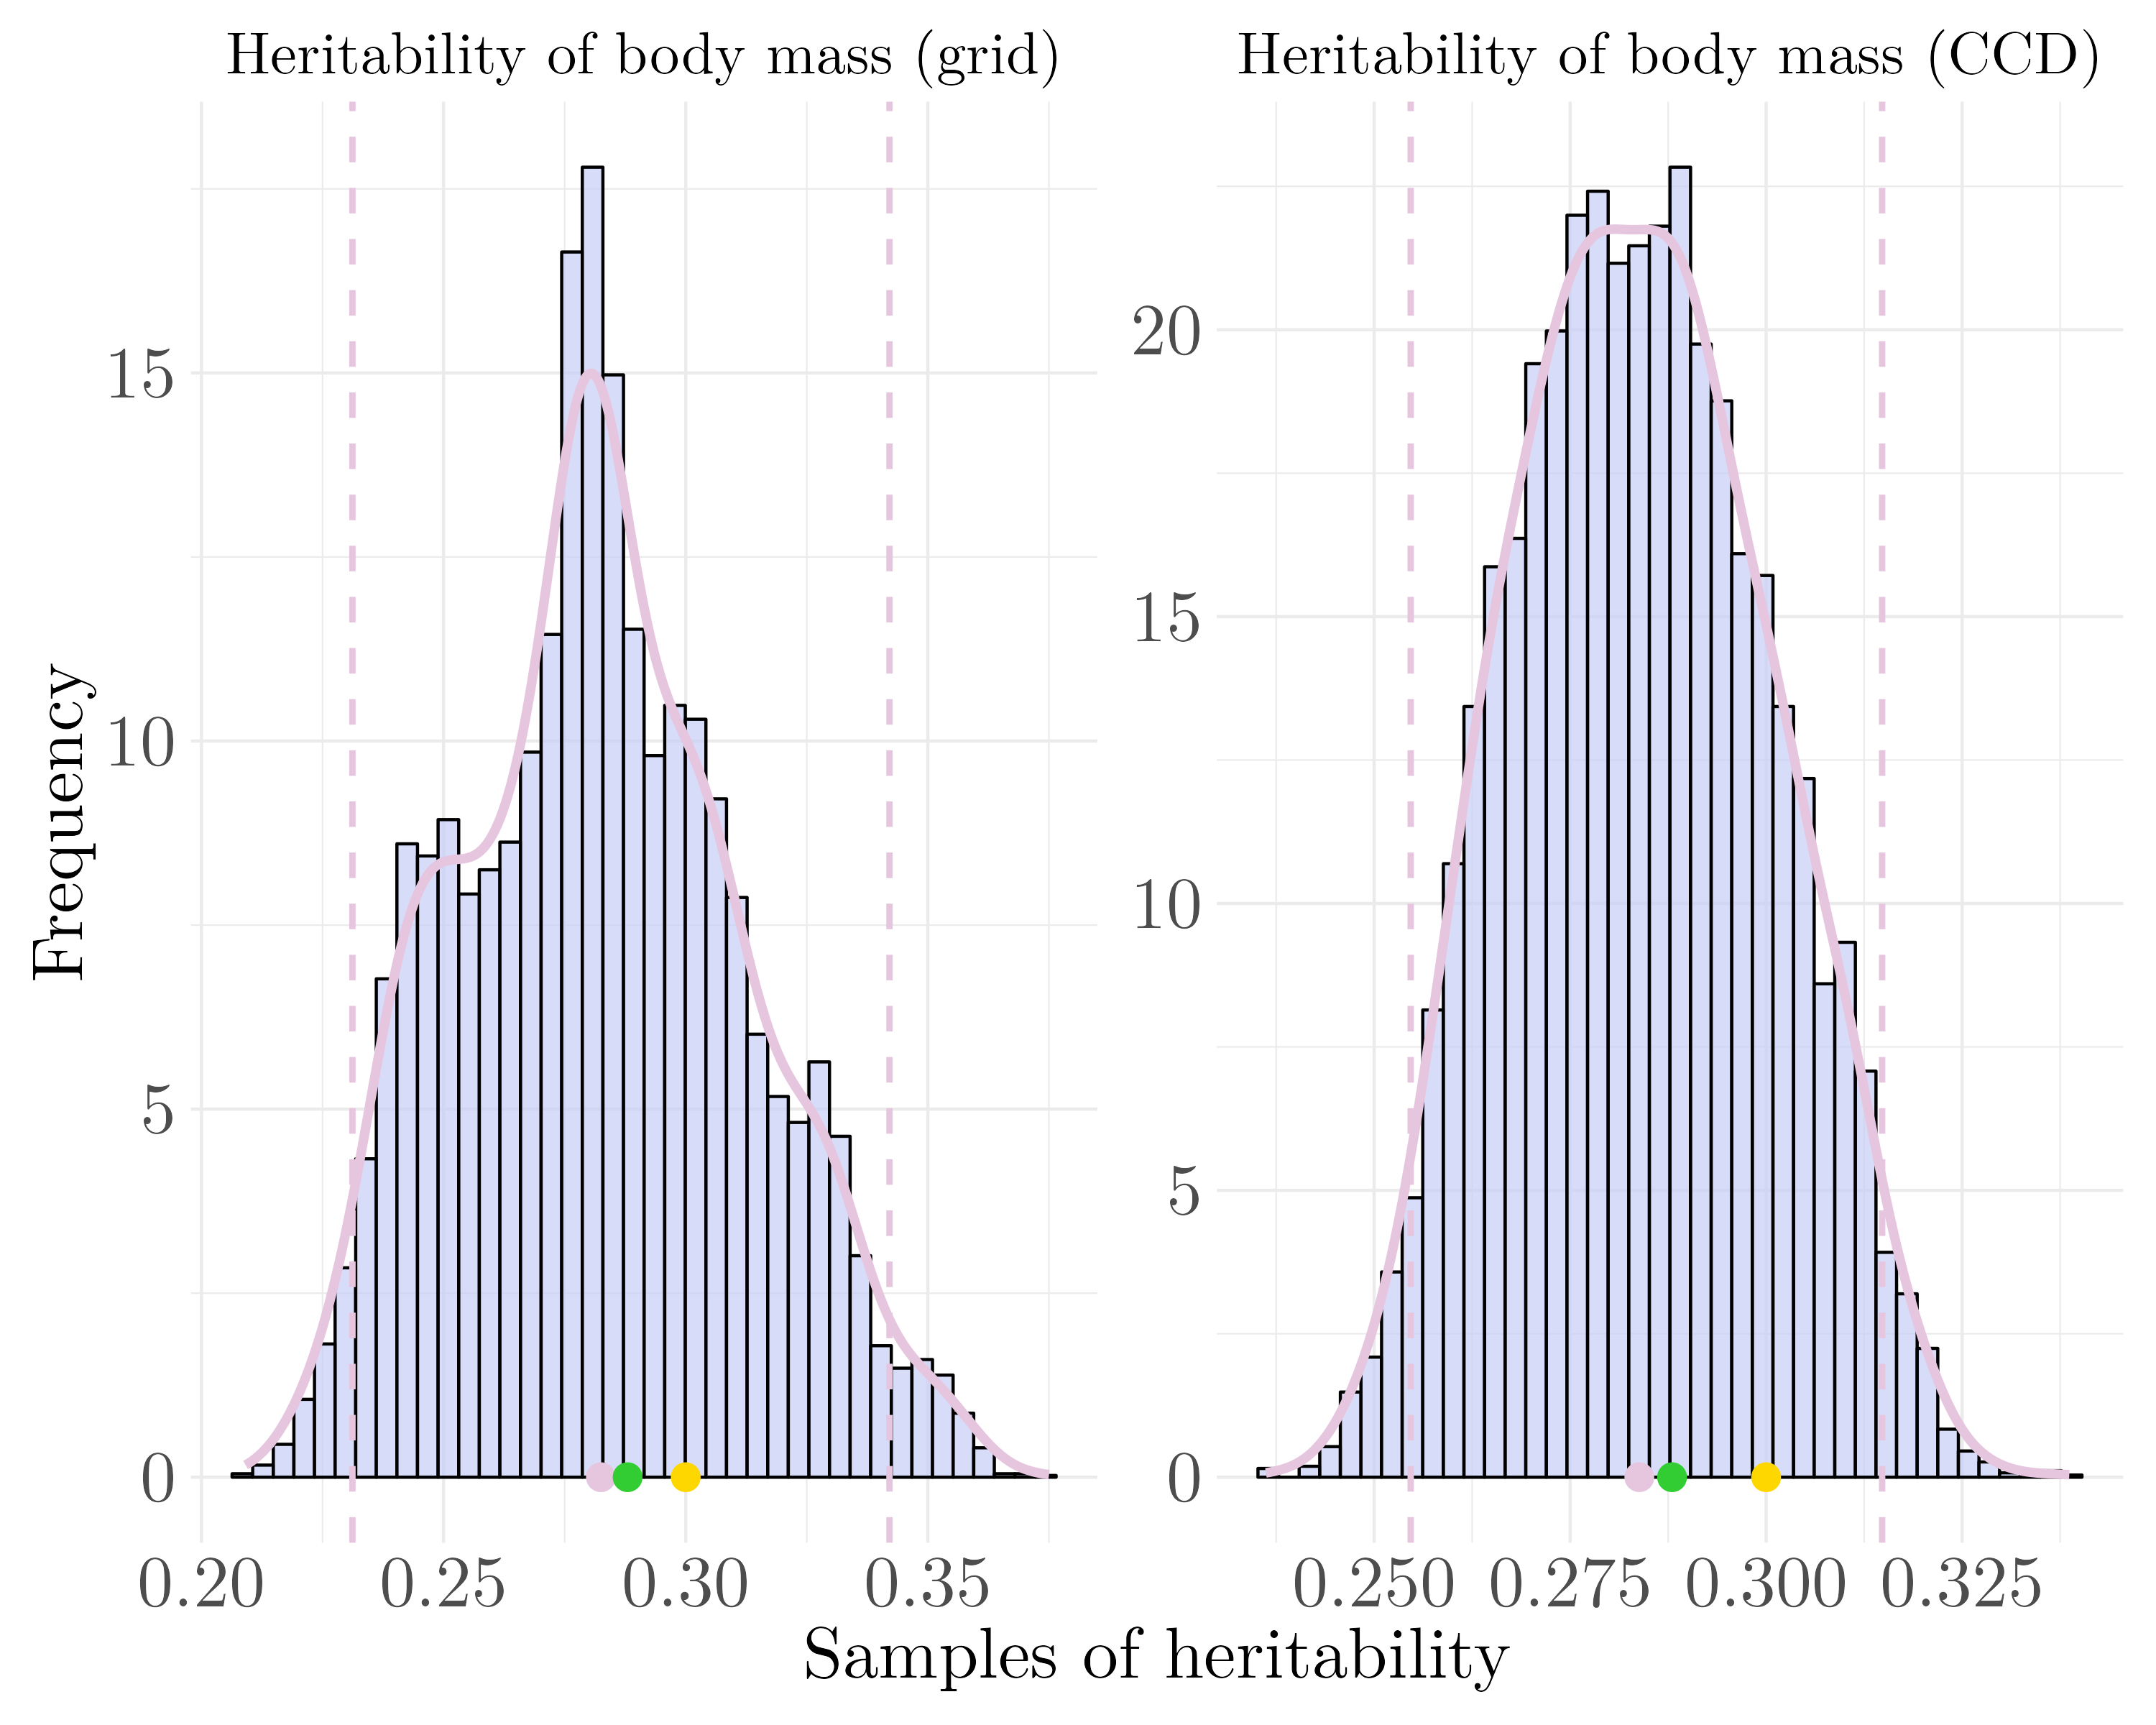
\includegraphics[width=0.7\linewidth]{Figures/House sparrow study/Heritability_mass_combined.png}
  \caption[Estimated heritability of body mass from grid and CCD strategy]{Histogram depicting the estimated heritability values of body mass by the BVI method for the grid integration strategy(left) and CCD integration strategy (right) for the house sparrow dataset. The mean of the samples is marked as a pink circle at the bottom of the histogram, with the lower and upper value for the $95\%$ percentile marked as dashed lines. The heritability estimate from \citet{Silva2017} and \citet{Muff2019Genetic} are marked as gold and green dots respectively at the bottom of the histogram.}
  \label{fig:heritability_mass_combined_grid_ccd}
\end{figure}

\begin{figure}[ht]
  \centering
  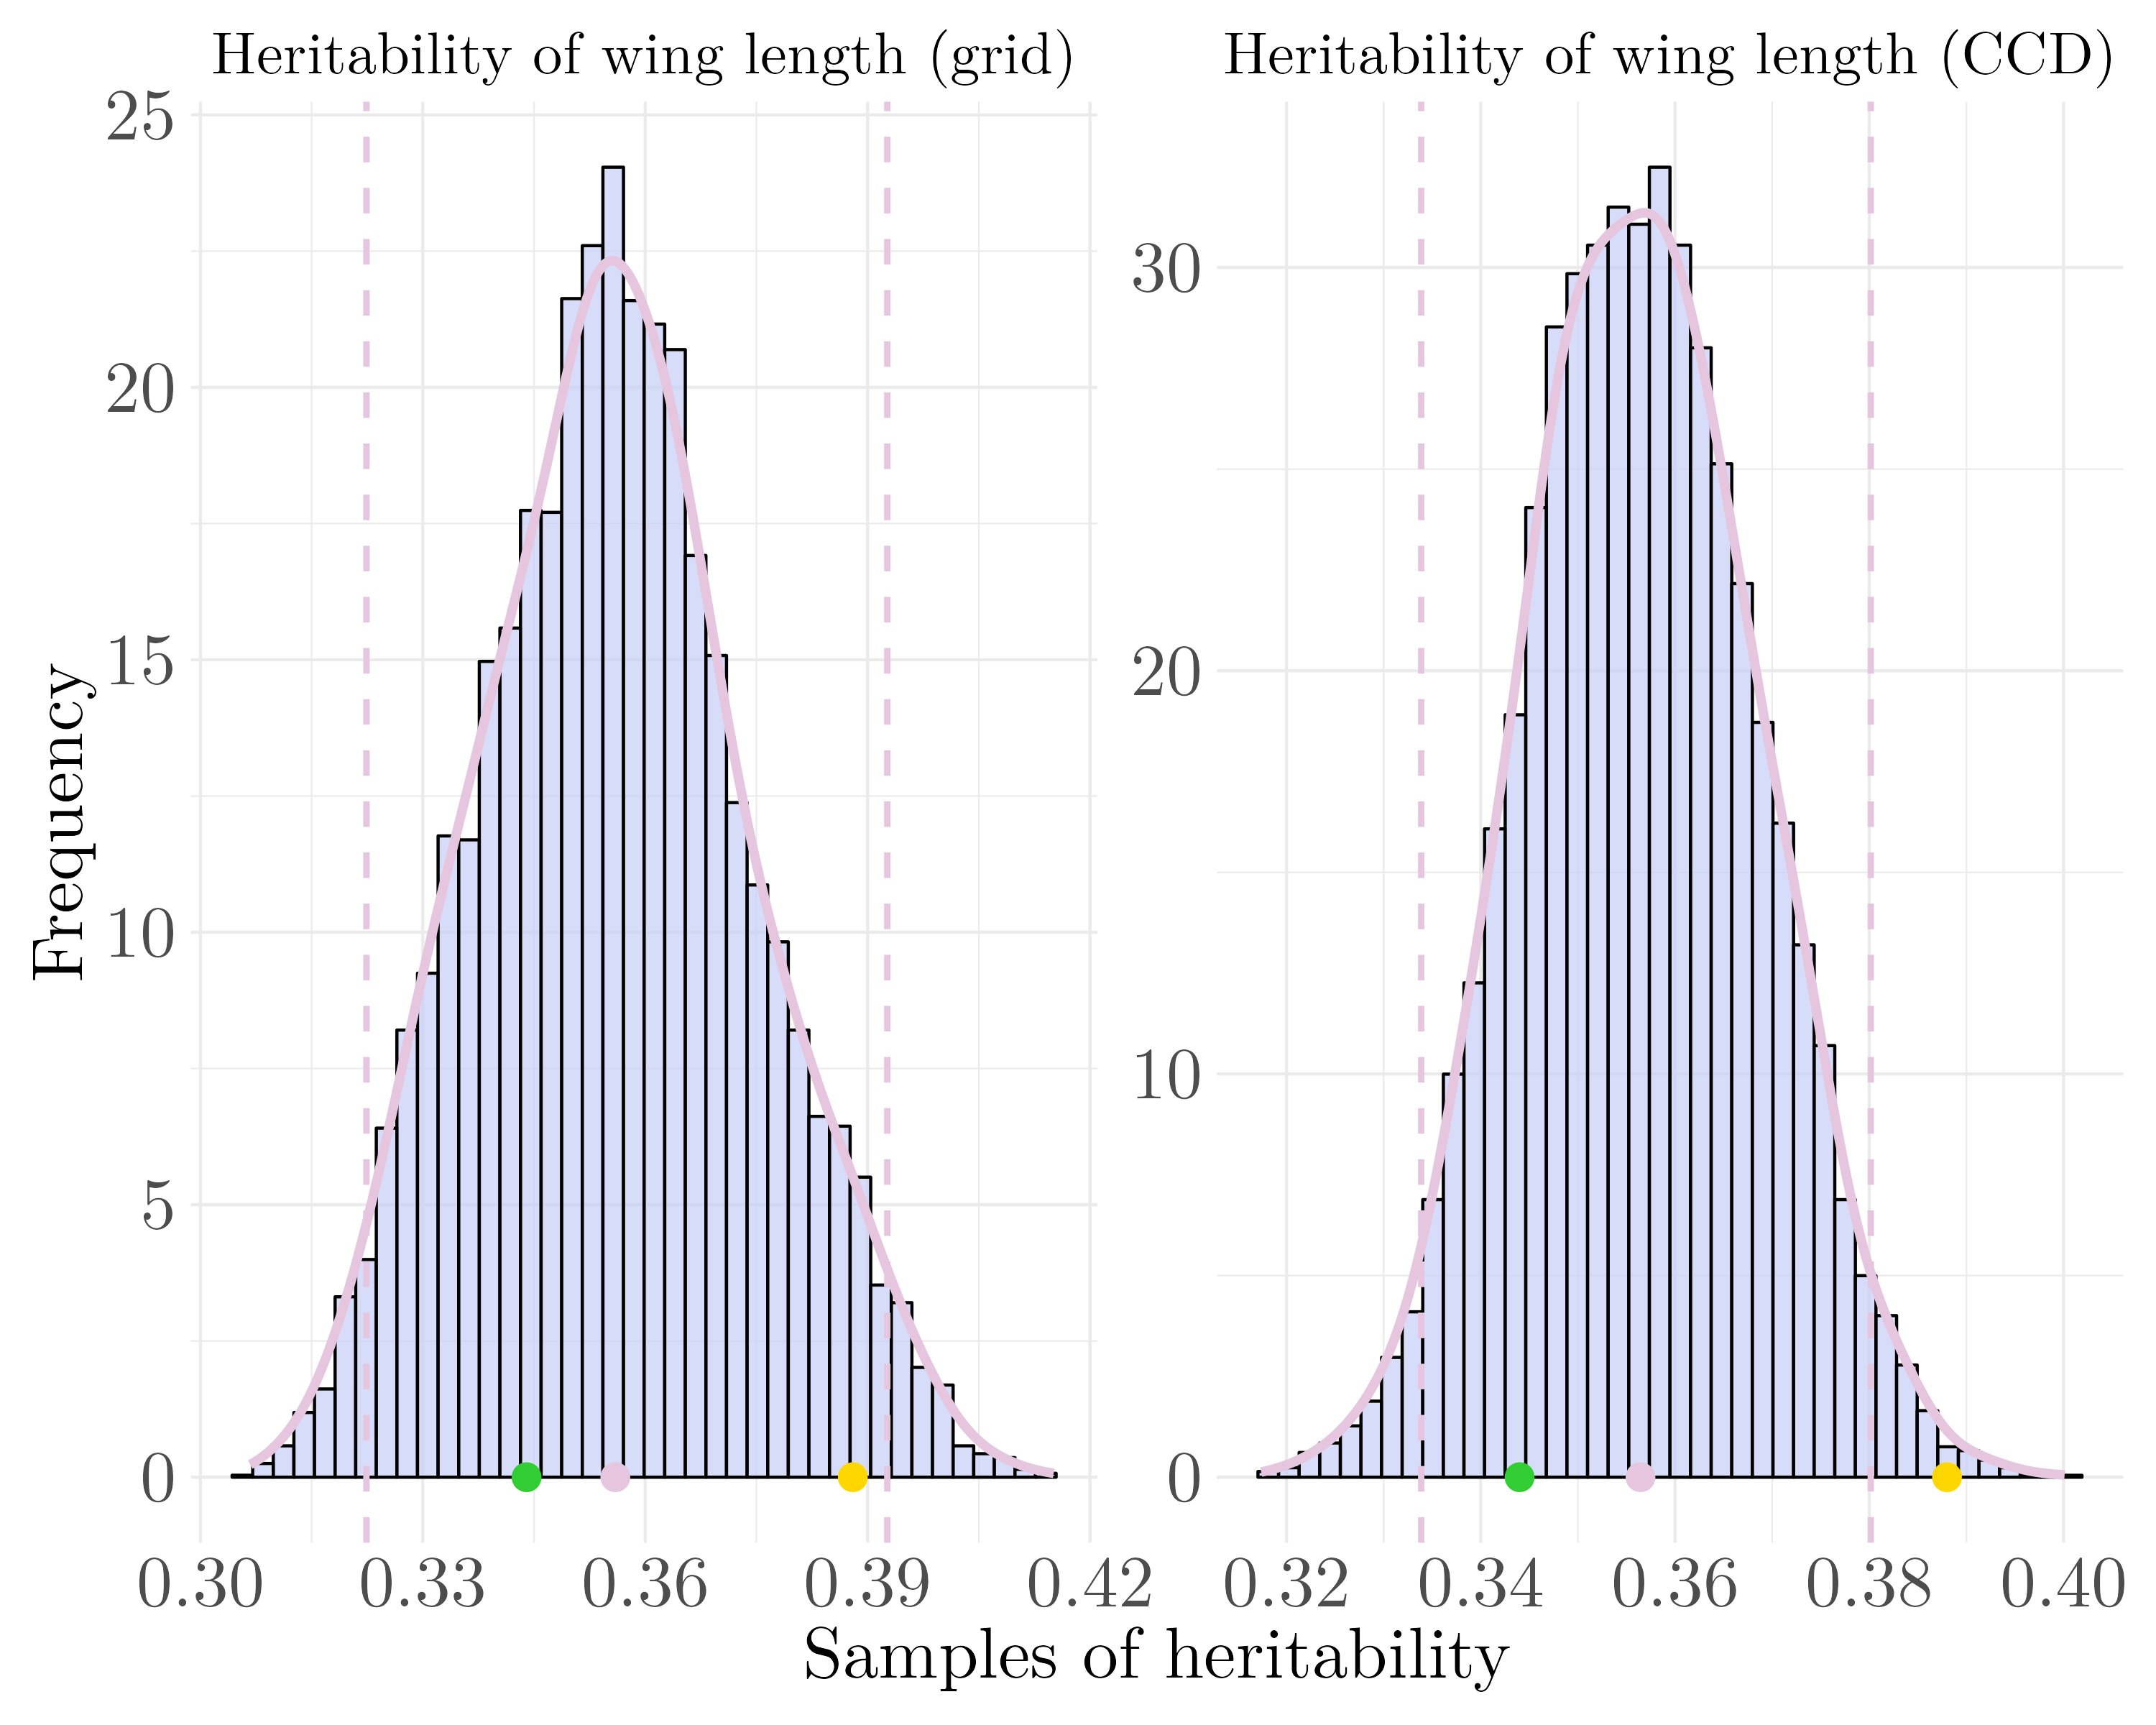
\includegraphics[width=0.7\linewidth]{Figures/House sparrow study/Heritability_wing_combined.png}
  \caption[Estimated heritability of wing length]{Histogram of heritability values for wing length of the house sparrows estimated by the BVI method for the grid integration strategy (left) and the CCD integration strategy (right). The mean of the samples is marked as a pink circle at the bottom of the histogram, and the lower and upper value for the $95\%$ percentile are featured as dashed lines. The heritability estimate from \citet{Silva2017} and \citet{Muff2019Genetic} are marked as gold and green dots respectively at the bottom of the histogram.}
  \label{fig:heritability_wing_combined_grid_ccd}
\end{figure}

\begin{figure}[H]
  \centering
  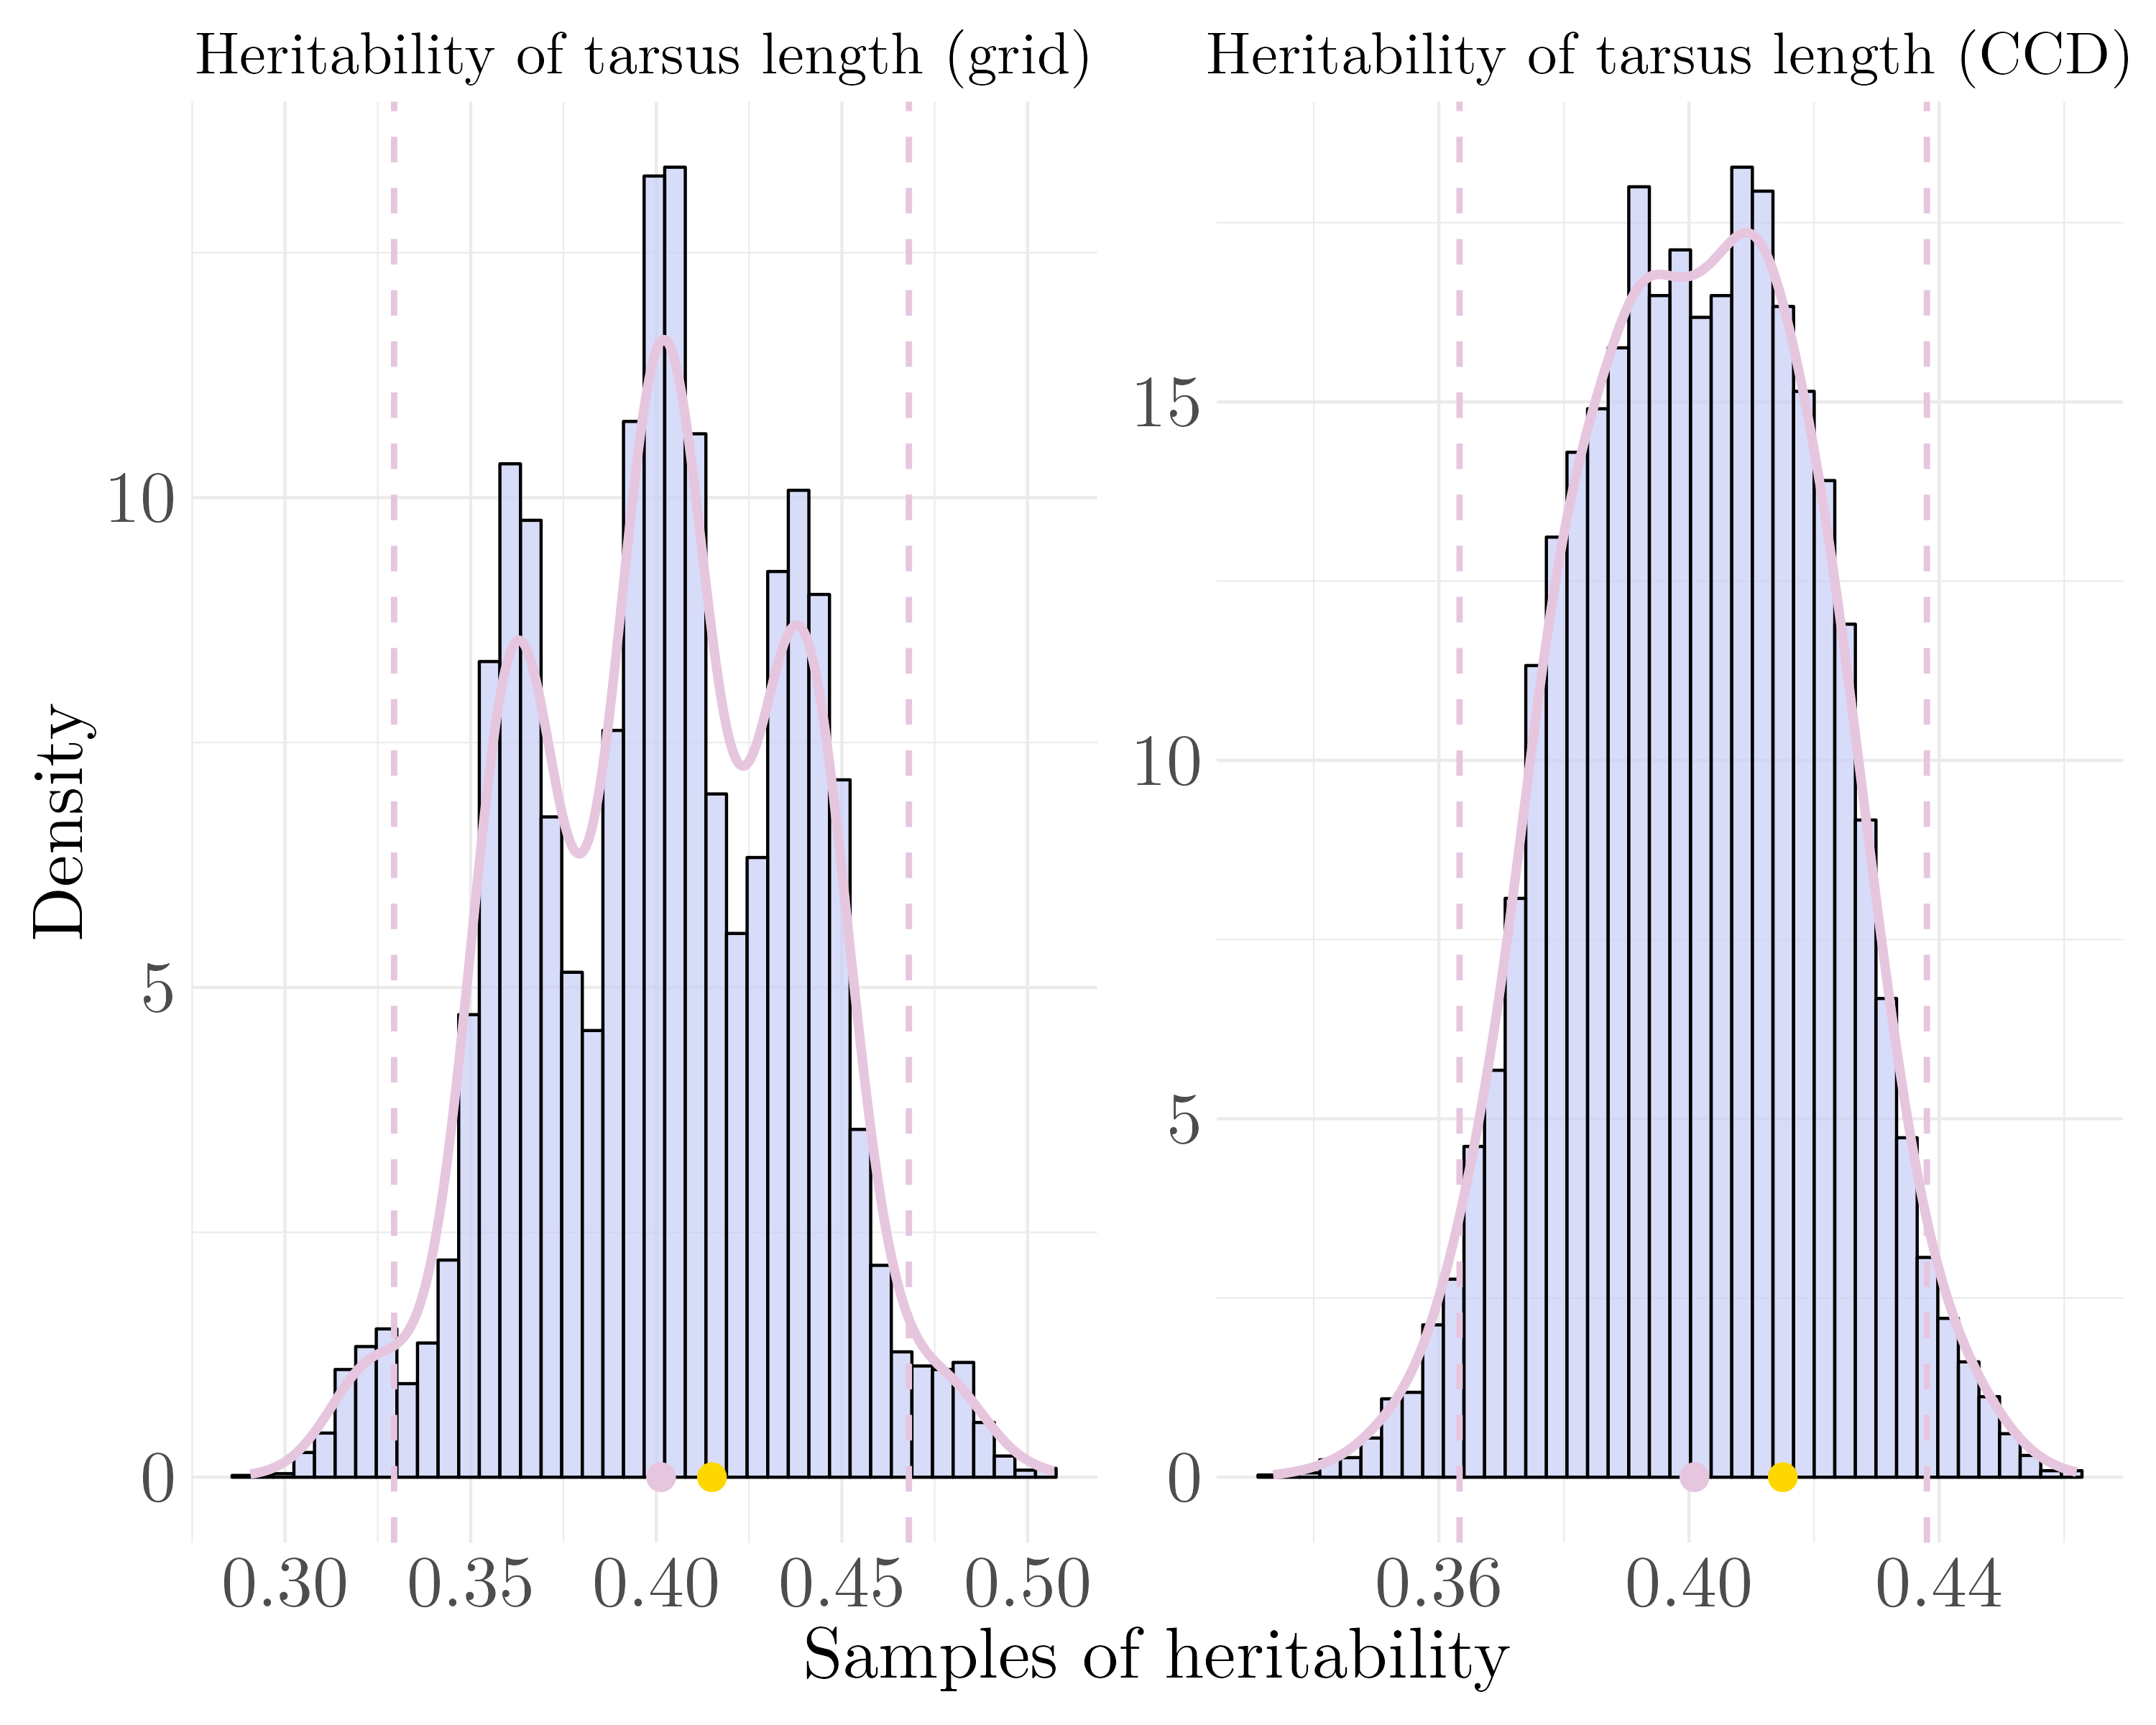
\includegraphics[width=0.7\linewidth]{Figures/House sparrow study/Heritability_tarsus_combined.png}
  \caption[Estimated heritability of tarsus length]{Histogram showing estimated heritability values for tarsus length of the house sparrows from the BVI method for the grid integration strategy (left) and the CCD integration strategy (right). The two dots at the bottom represent the mean of the samples (pink) and the estimate from \citep{Silva2017} (gold). The dashed lines represent the lower and upper value for the $95\%$ percentile.}
  \label{fig:heritability_tarsus_combined_grid_ccd}
\end{figure}
% \\
% \\
% The posterior distribution of relative importance of the fixed effects (\Cref{fig:mass_fixed_sparrows}) predominantly shows very small values. Both integration strategies yield very similar distributions. Notably, the covariates \textit{FGRM, age} and \textit{other} seem to have been allocated negligible importance, with the distributions of \textit{FGRM} and \textit{other} exhibiting a negative exponential decay pattern. Recall that importance calculations include squaring the coefficients, and so no negative importance can be allocated to a covariate. Therefore, the sharp decay from zero seems reasonable. The covariates \textit{month, sex} and \textit{outer} seem to have been allocated a small share of the importance, with \textit{month} and \textit{sex} showing signs of a normal distribution.
% \begin{figure}[H]%\ContinuedFloat
%   \centering
%   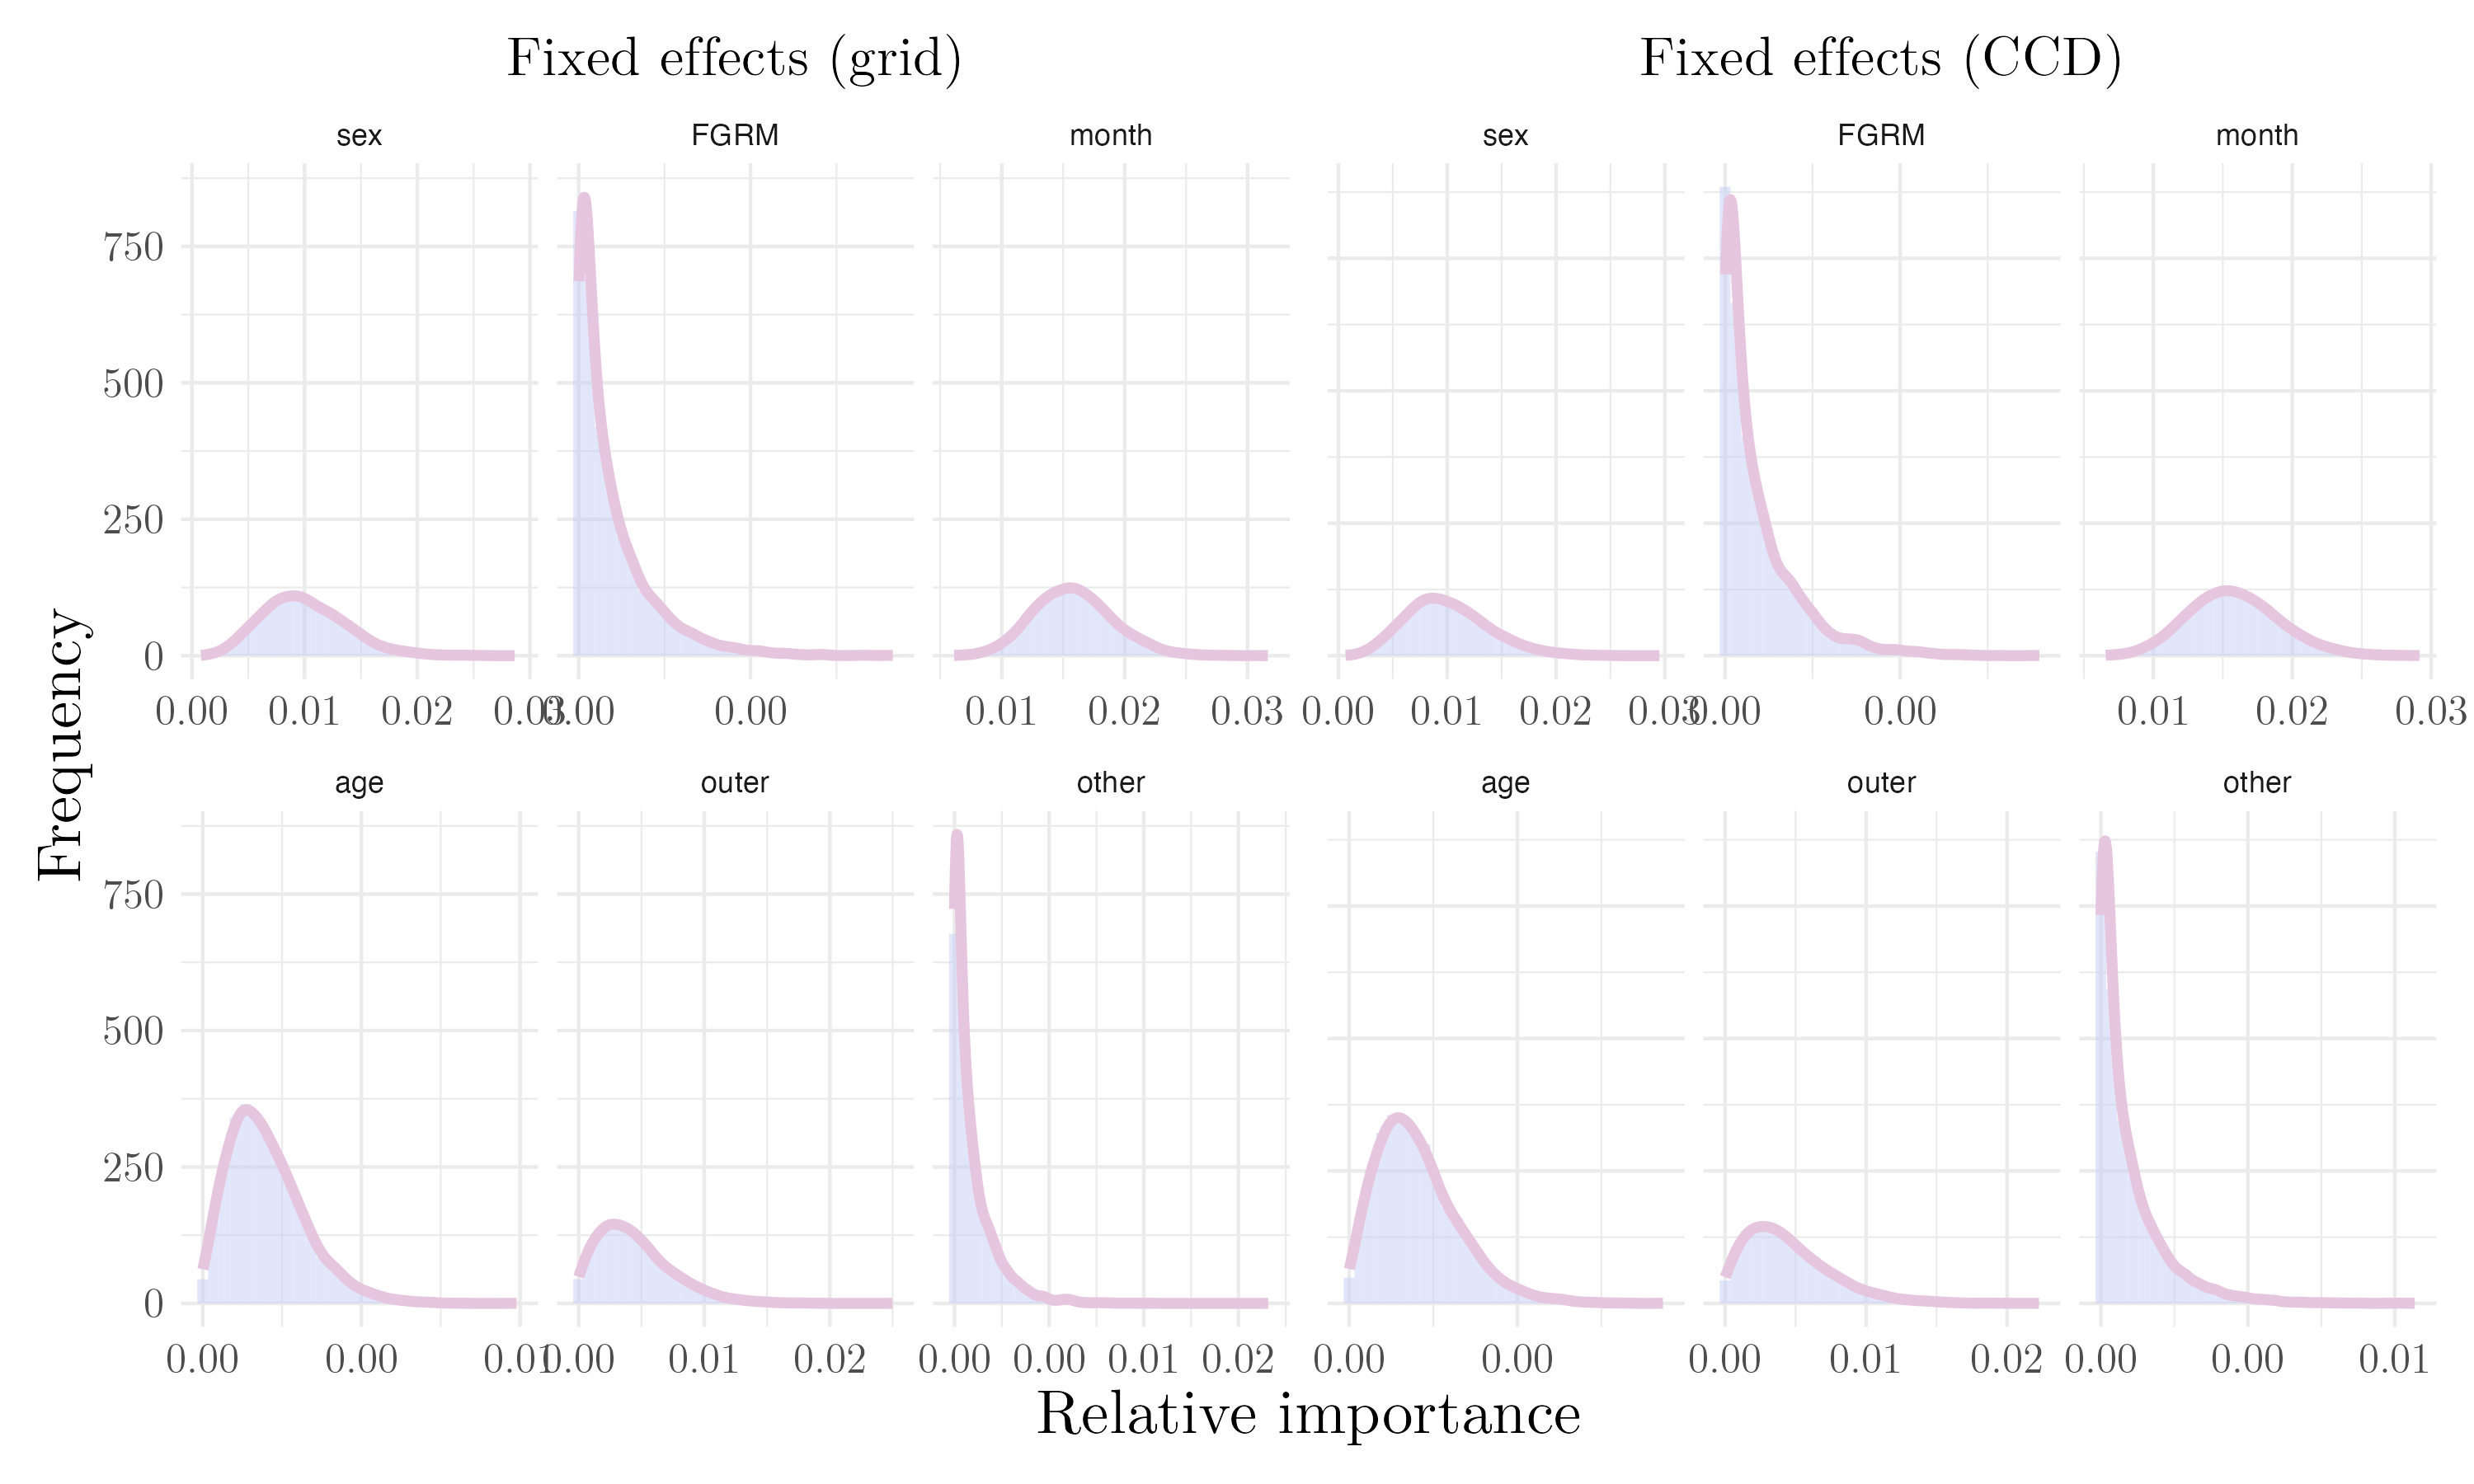
\includegraphics[width=1\linewidth]{Figures/House sparrow study/Mass_fixed.png}
%   \caption[Posterior relative importance distributions of all fixed effects in body mass model for house sparrow study]{Posterior relative importance distributions of all fixed effects in heritability of body mass model for house sparrow study. The grid integration is displayed on the left, and CCD on the right.}
%   \label{fig:mass_fixed_sparrows}
% \end{figure}
% When considering the posterior importance of the random effects (\Cref{fig:mass_random_sparrows}), it is evident that they have been allocated a much larger share of importance compared to the fixed effects. The Gaussian observations exhibit the largest influence, being allocated a share of over $0.5$ in both integration strategies. It seems that the CCD integration gives somewhat smoother distributions, but the mean values seem to be roughly similar. We notice a trimodal shape for the individual effect \textit{IDC} (overdispersion) with the grid integration strategy, similar to that observed for the heritability of tarsus length. The smallest importance of random effects is allocated to \textit{hatchyear}, and the estimates for covariate \textit{IDC2} corresponds to the heritability of body mass.
% \begin{figure}[H]%\ContinuedFloat
%   \centering
%   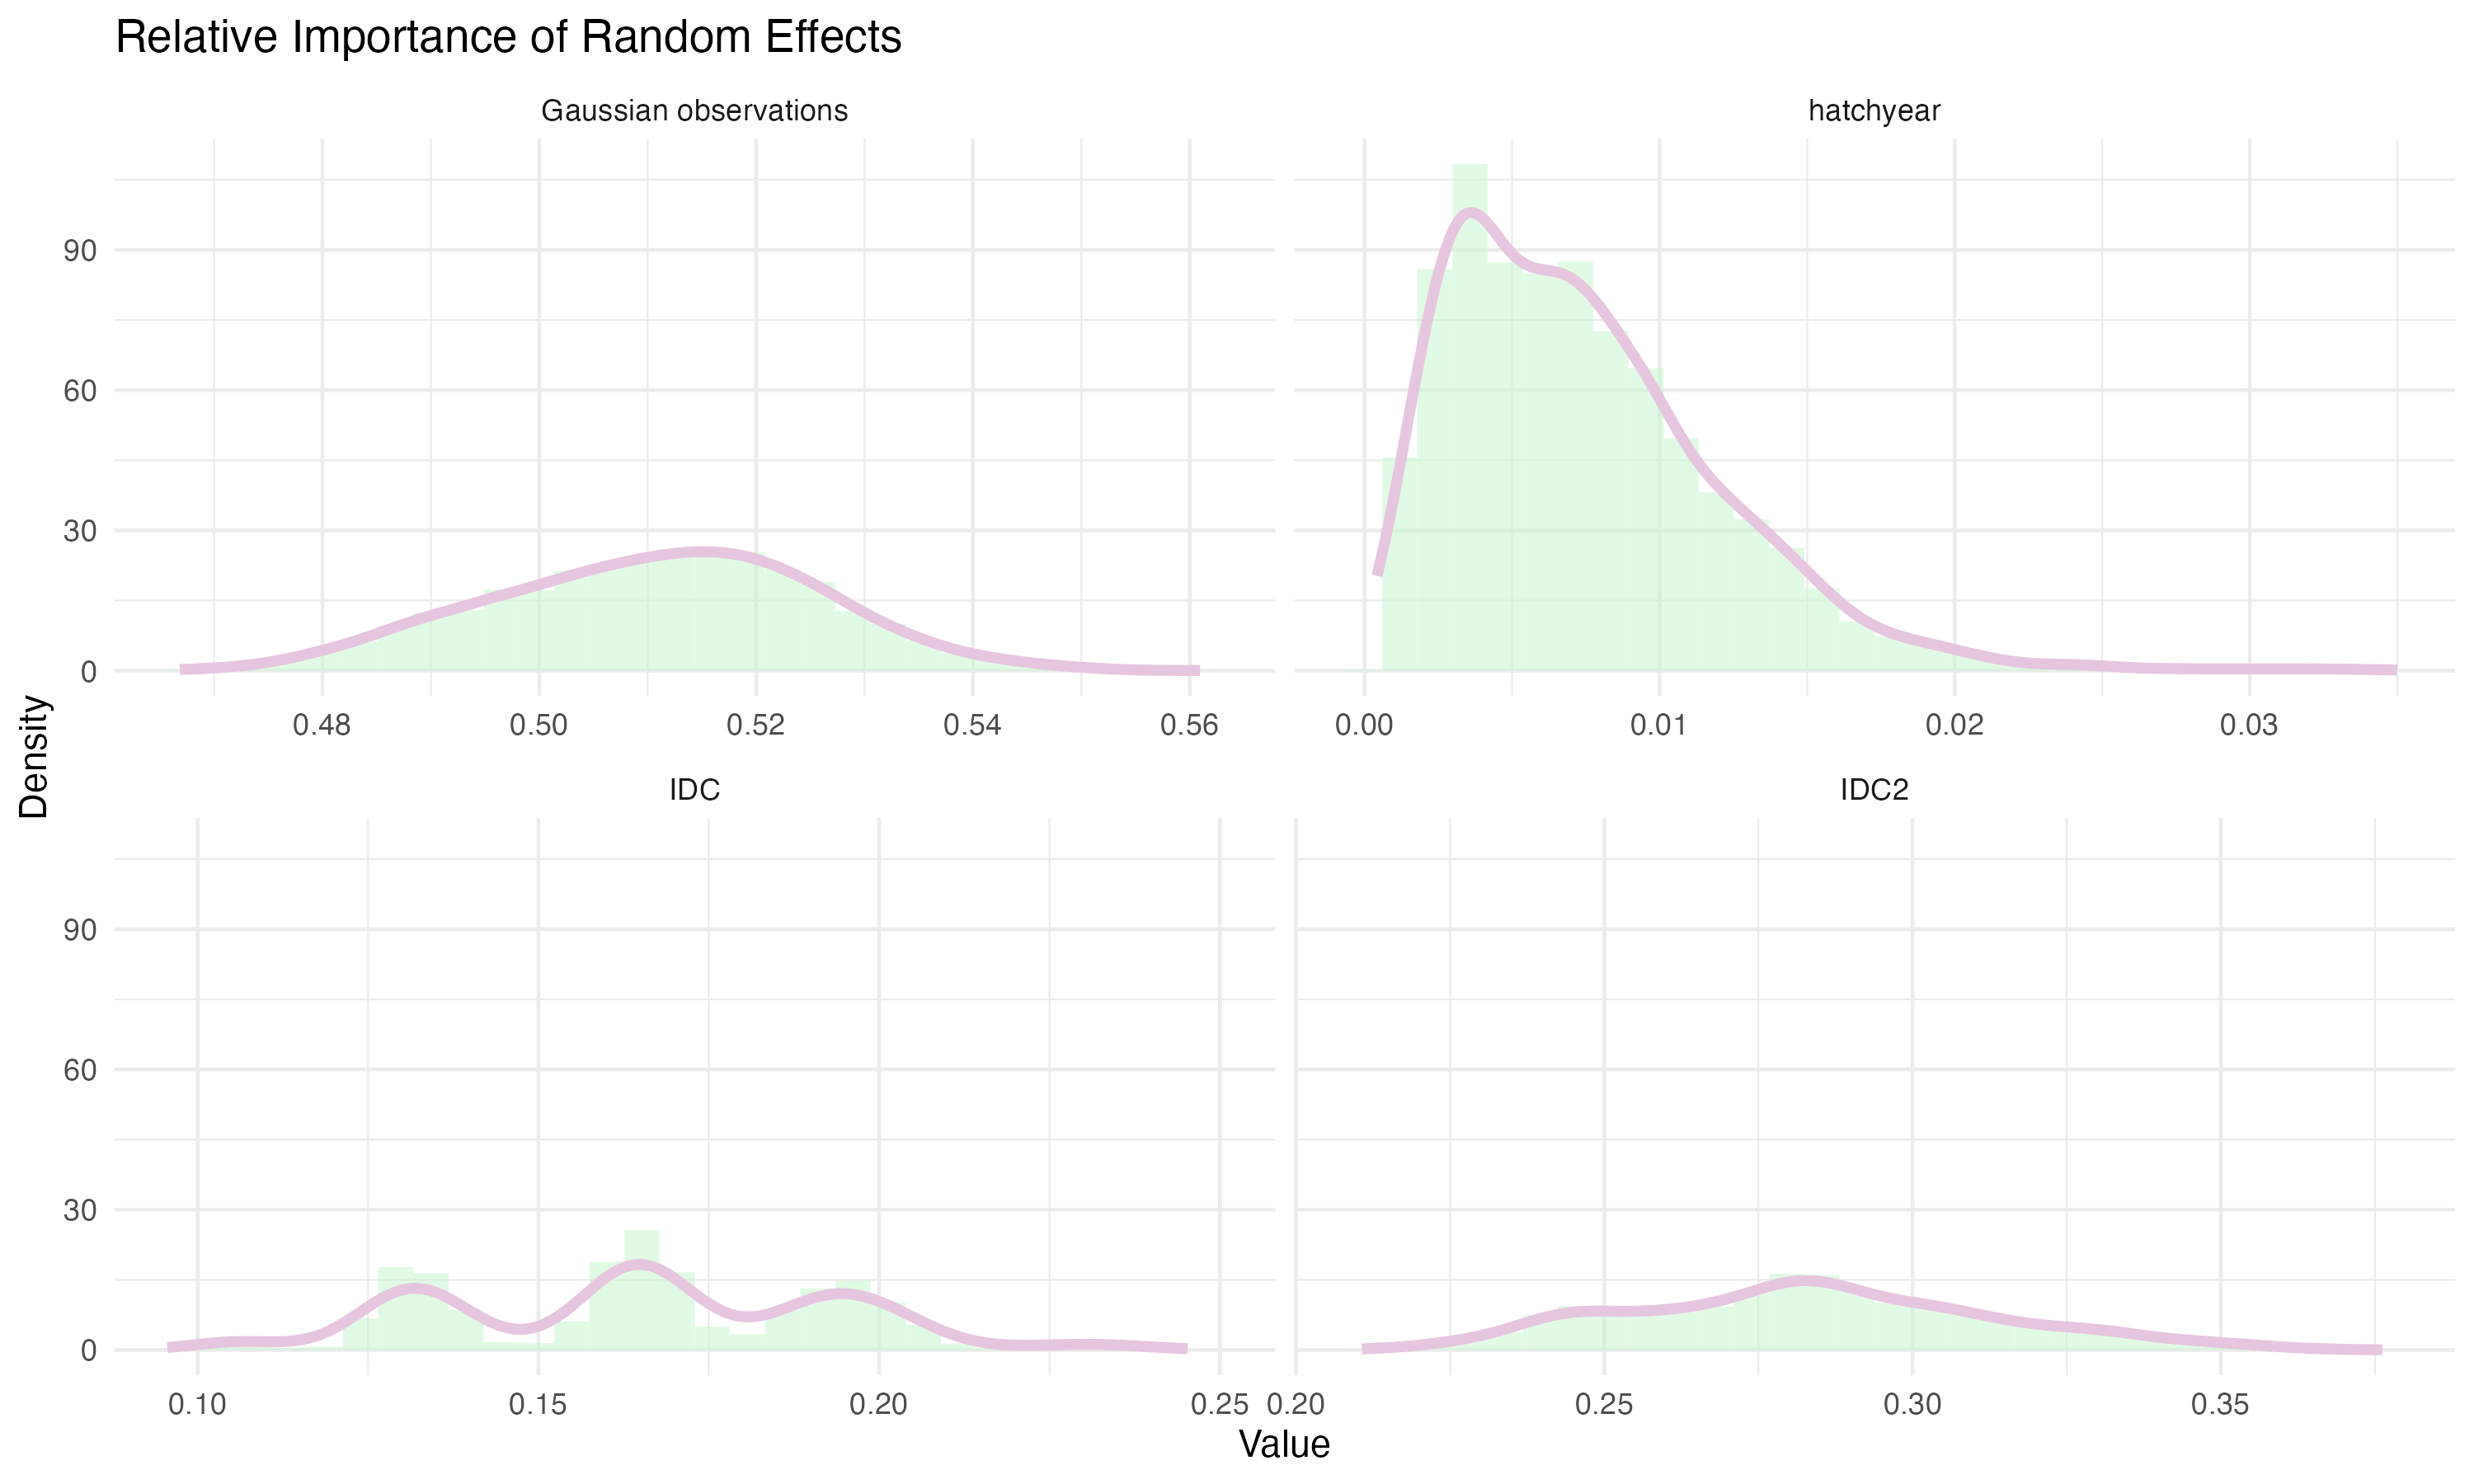
\includegraphics[width=1\linewidth]{Figures/House sparrow study/Mass_random.png}
%   \caption[Posterior relative importance distributions of all random effects in body mass model for house sparrow study]{Posterior relative importance distributions of all random effects in heritability of body mass model for house sparrow study. The grid integration is displayed on the left, and CCD on the right.}
%   \label{fig:mass_random_sparrows}
% \end{figure}
% As the marginal $R^2$ is the sum of the importance of fixed effects, the resulting estimates (\Cref{fig:mass_r2}) are expectedly very small. The conditional $R^2$ estimates are much larger, which is because this contains the importances of the random effects. All in all, the grid and CCD integrations yield similar results, with a slightly sharper peak for the conditional $R^2$ by the CCD integration. 
% \begin{figure}[H]%\ContinuedFloat
%   \centering
%   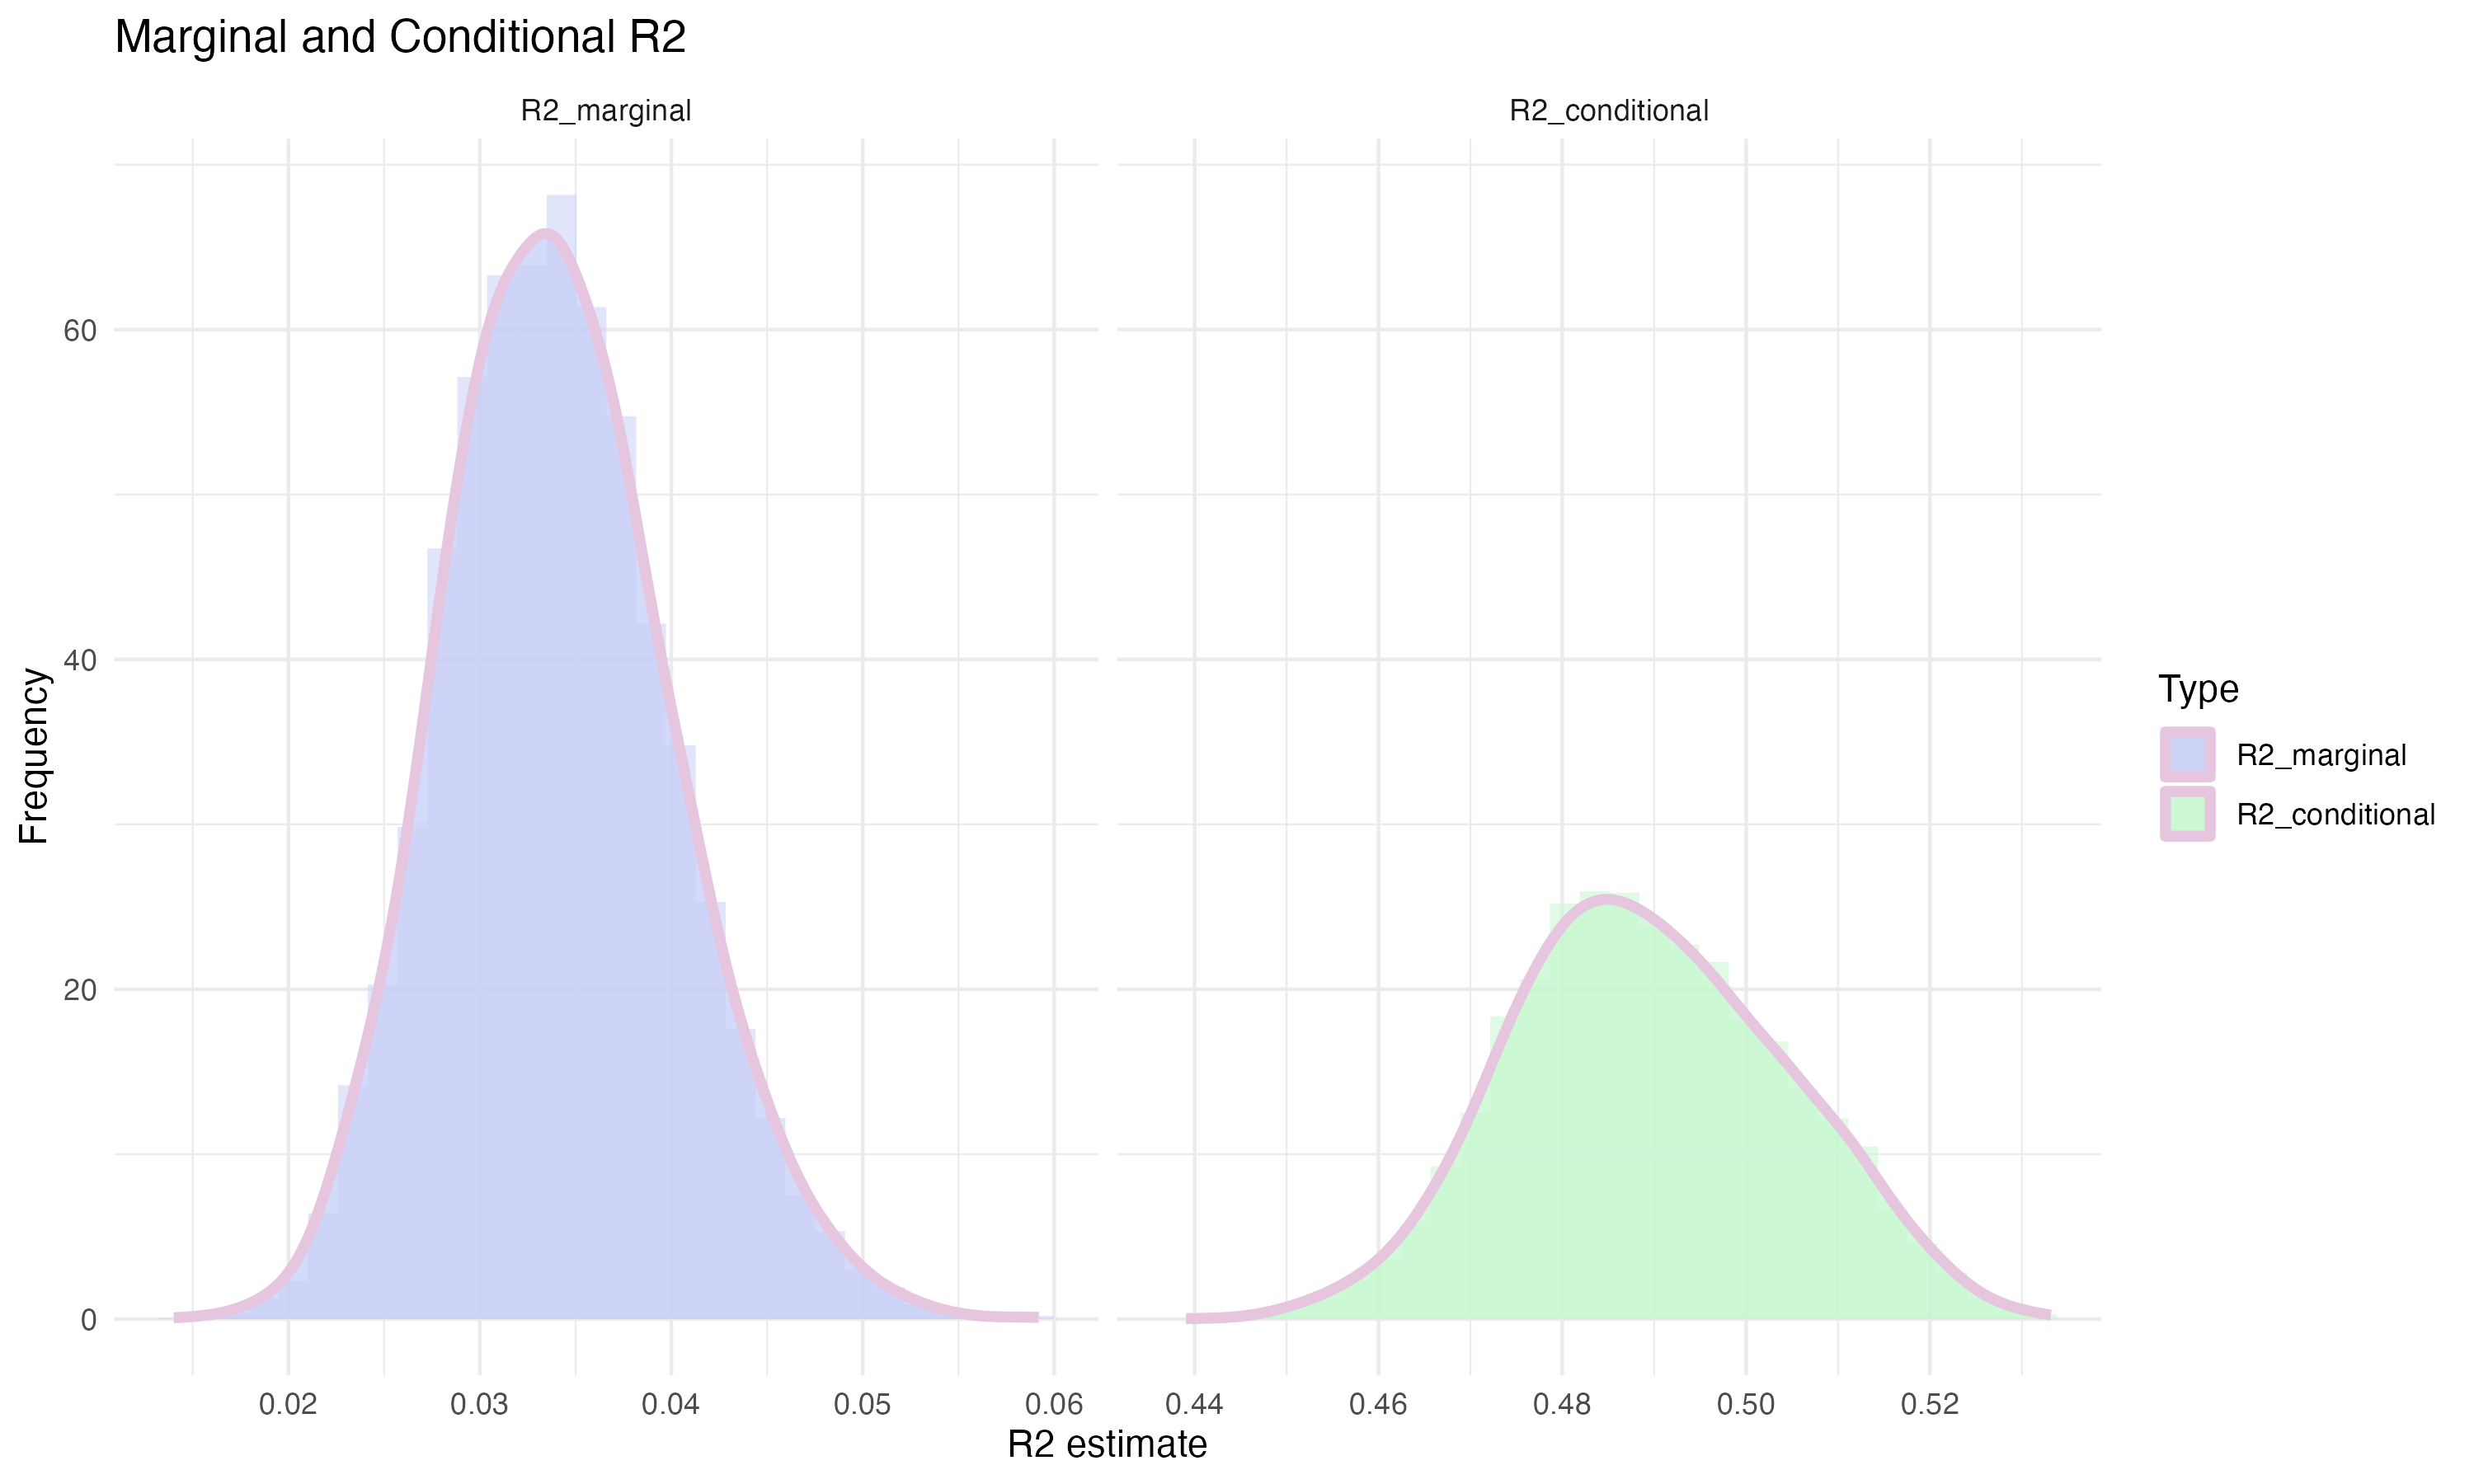
\includegraphics[width=1\linewidth]{Figures/House sparrow study/Mass_r2.png}
%   \caption[Posterior distributions of $R^2$ values in body mass model for house sparrow study]{Posterior distributions of $R^2$ values in heritability of body mass model for house sparrow study. The grid integration is displayed on the left, and CCD on the right.}
%   \label{fig:mass_r2}
% \end{figure}
% As for the fixed effects of the body mass model, the posterior importance of random effects for wing length (\Cref{fig:wing_fixed_sparrows}) are also generally very small except for the covariate \textit{sex}. The importance of covariate \textit{sex} seems to be normal around a value just below $0.35$, which is significantly larger than all other random effects. For wing length, \textit{FGRM} and \textit{other} are allocated a negligible importance, however they do not have the same negative exponential pattern as for body mass. Again, both integration strategies are in close agreement.
% \begin{figure}[H]%\ContinuedFloat
%   \centering
%   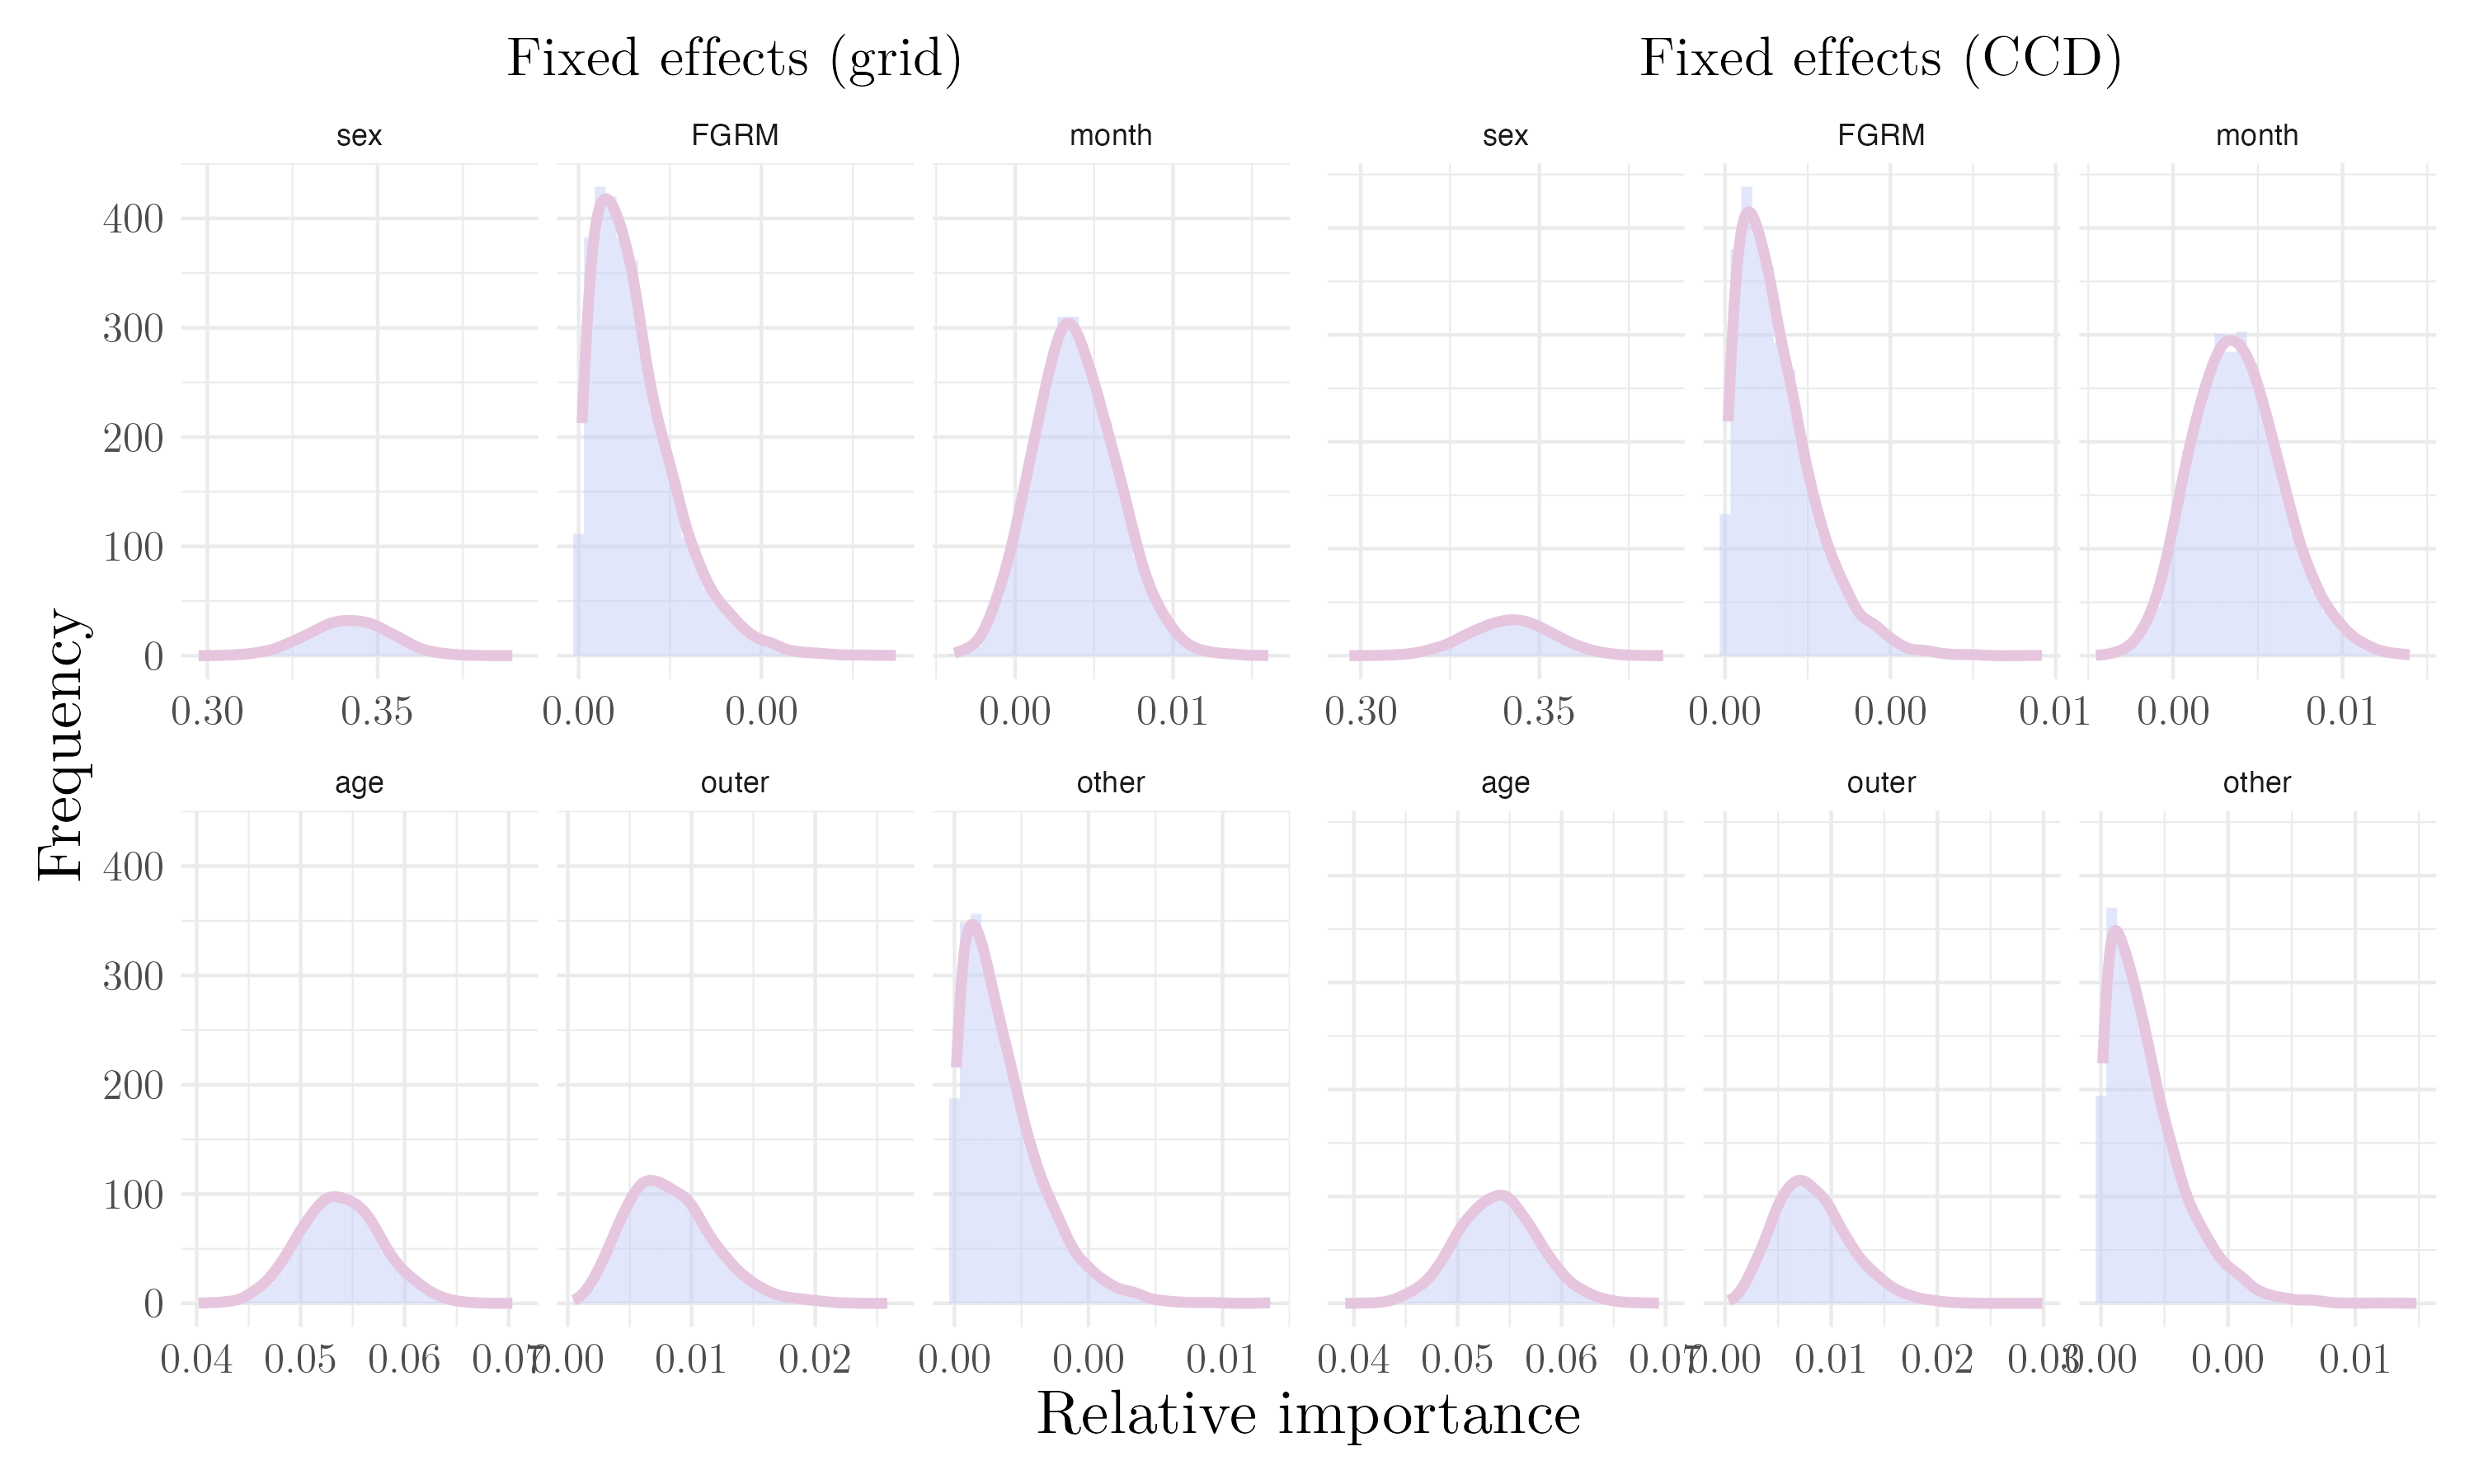
\includegraphics[width=1\linewidth]{Figures/House sparrow study/Wing_fixed.png}
%   \caption[Posterior relative importance distributions of all fixed effects in wing length model for house sparrow study]{Posterior relative importance distributions of all fixed effects in wing length model for house sparrow study. The grid integration is displayed on the left, and CCD on the right.}
%   \label{fig:wing_fixed_sparrows}
% \end{figure}
% For posterior importance of the random effects in the model for wing length (\Cref{fig:wing_random_sparrows}), the Gaussian observations are given an importance distributed around $0.175$. This is smaller than for body mass, and the \textit{IDC} covariate is also attributed significantly less importance when modelling wing length. The importance of \textit{hatchyear} is again quite small, and the importance of \textit{IDC2} (heritability) is now distributed around $0.36$. Once more, we observe the trimodal pattern for the importance of \textit{IDC} with the grid strategy. The CCD integrations also shows signs of a trimodal pattern for \textit{IDC}, but the peaks are less pronounced. 
% \begin{figure}[H]%\ContinuedFloat
%   \centering
%   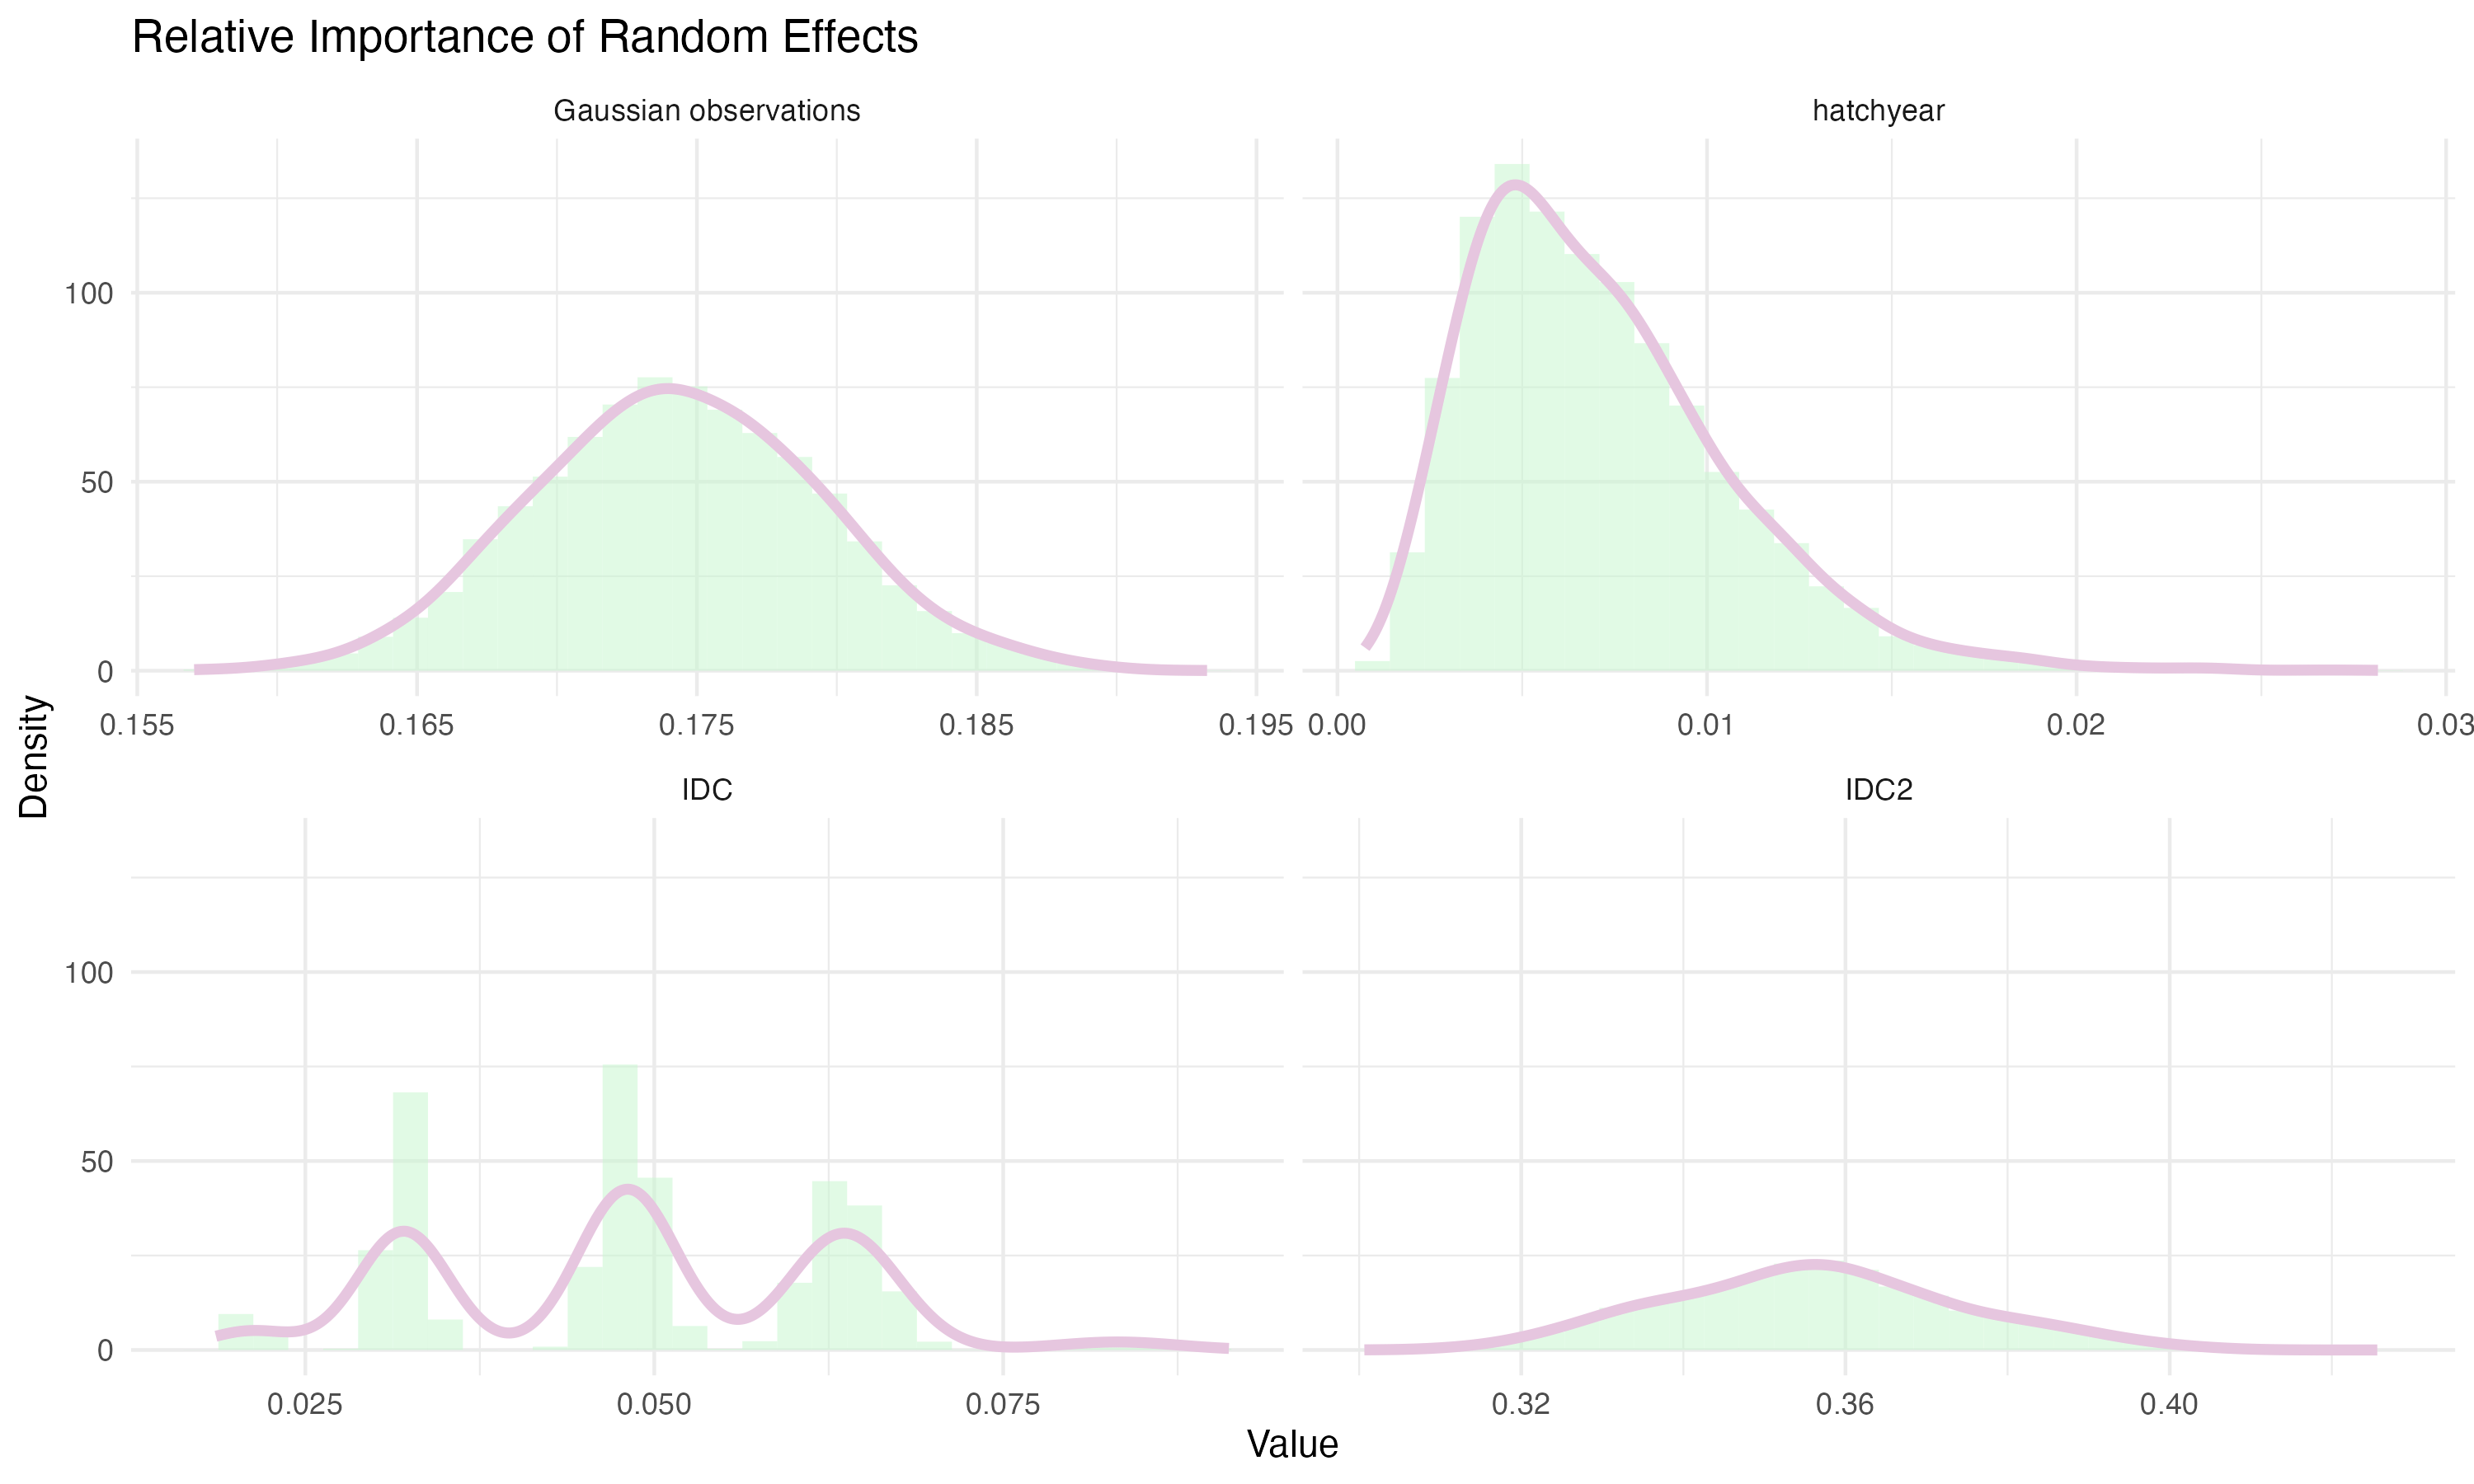
\includegraphics[width=1\linewidth]{Figures/House sparrow study/Wing_random.png}
%   \caption[Posterior relative importance distributions of all random effects in wing length model for house sparrow study]{Posterior relative importance distributions of all random effects in heritability of wing length model for house sparrow study. The grid integration is displayed on the left, and CCD on the right.}
%   \label{fig:wing_random_sparrows}
% \end{figure}
% Both the marginal and conditional $R^2$ of the wing length model (\Cref{fig:wing_r2}) are relatively large, which is a consequence of \textit{sex} being allocated a larger importance and the smaller importance allocated to the Gaussian observations. In this case, the peaks of the $R^2$ values with CCD integration are slightly sharper than for the grid integration, but the overall patterns are consistent across both methods.
% \begin{figure}[H]%\ContinuedFloat
%   \centering
%   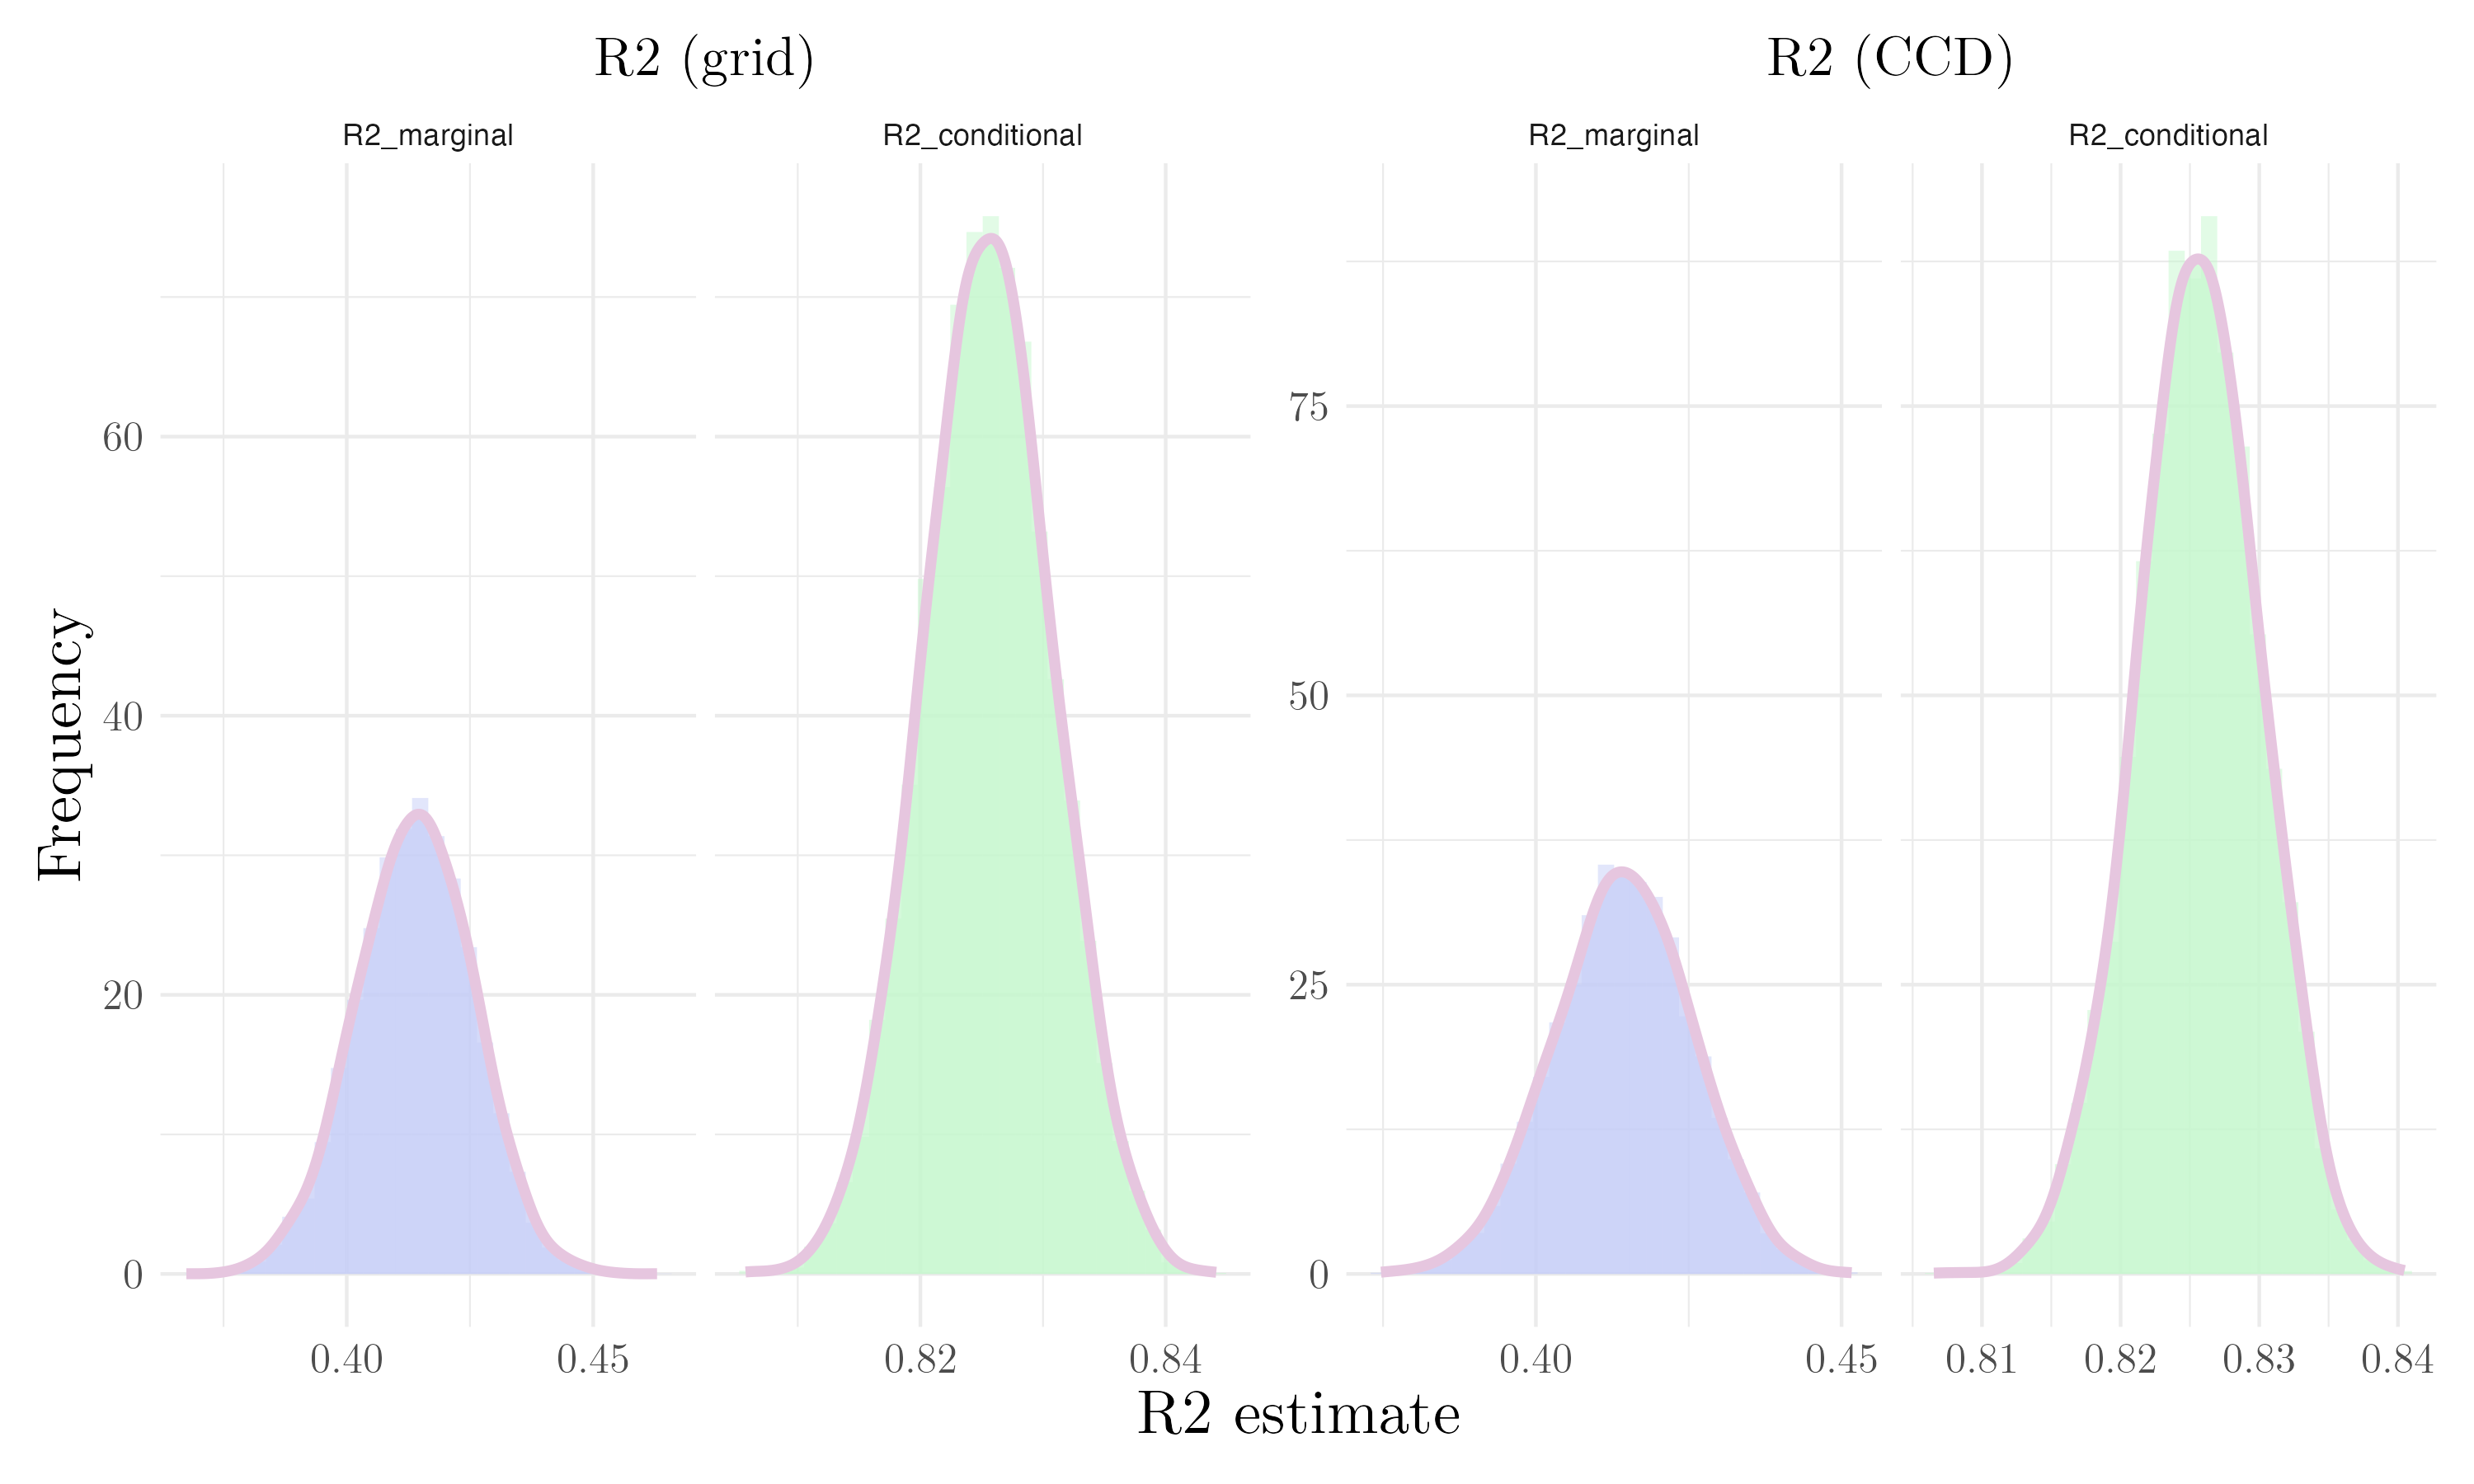
\includegraphics[width=1\linewidth]{Figures/House sparrow study/Wing_r2.png}
%   \caption[Posterior distributions of $R^2$ values in wing length model for house sparrow study]{Posterior distributions of $R^2$ values in heritability of wing length model for house sparrow study. The grid integration is displayed on the left, and CCD on the right.}
%   \label{fig:wing_r2}
% \end{figure}
% The posterior importance of fixed effects of the tarsus length model (\Cref{fig:tarsus_fixed_sparrows}) are challenging to interpret due to their minimal values. The covariate \textit{age} has a sharp decay right after zero with an extremely high frequency. Individually examining each importance distribution reveals that \textit{outer} and \textit{other} exhibit a negative exponential pattern, whereas \textit{month} follows a normal distribution.. Both \textit{sex} and \textit{FGRM} are very small and have a skewed normal distribution. It seems the integration strategies agree, and overall the fixed effects are given a very small importance.
% \begin{figure}[H]%\ContinuedFloat
%   \centering
%   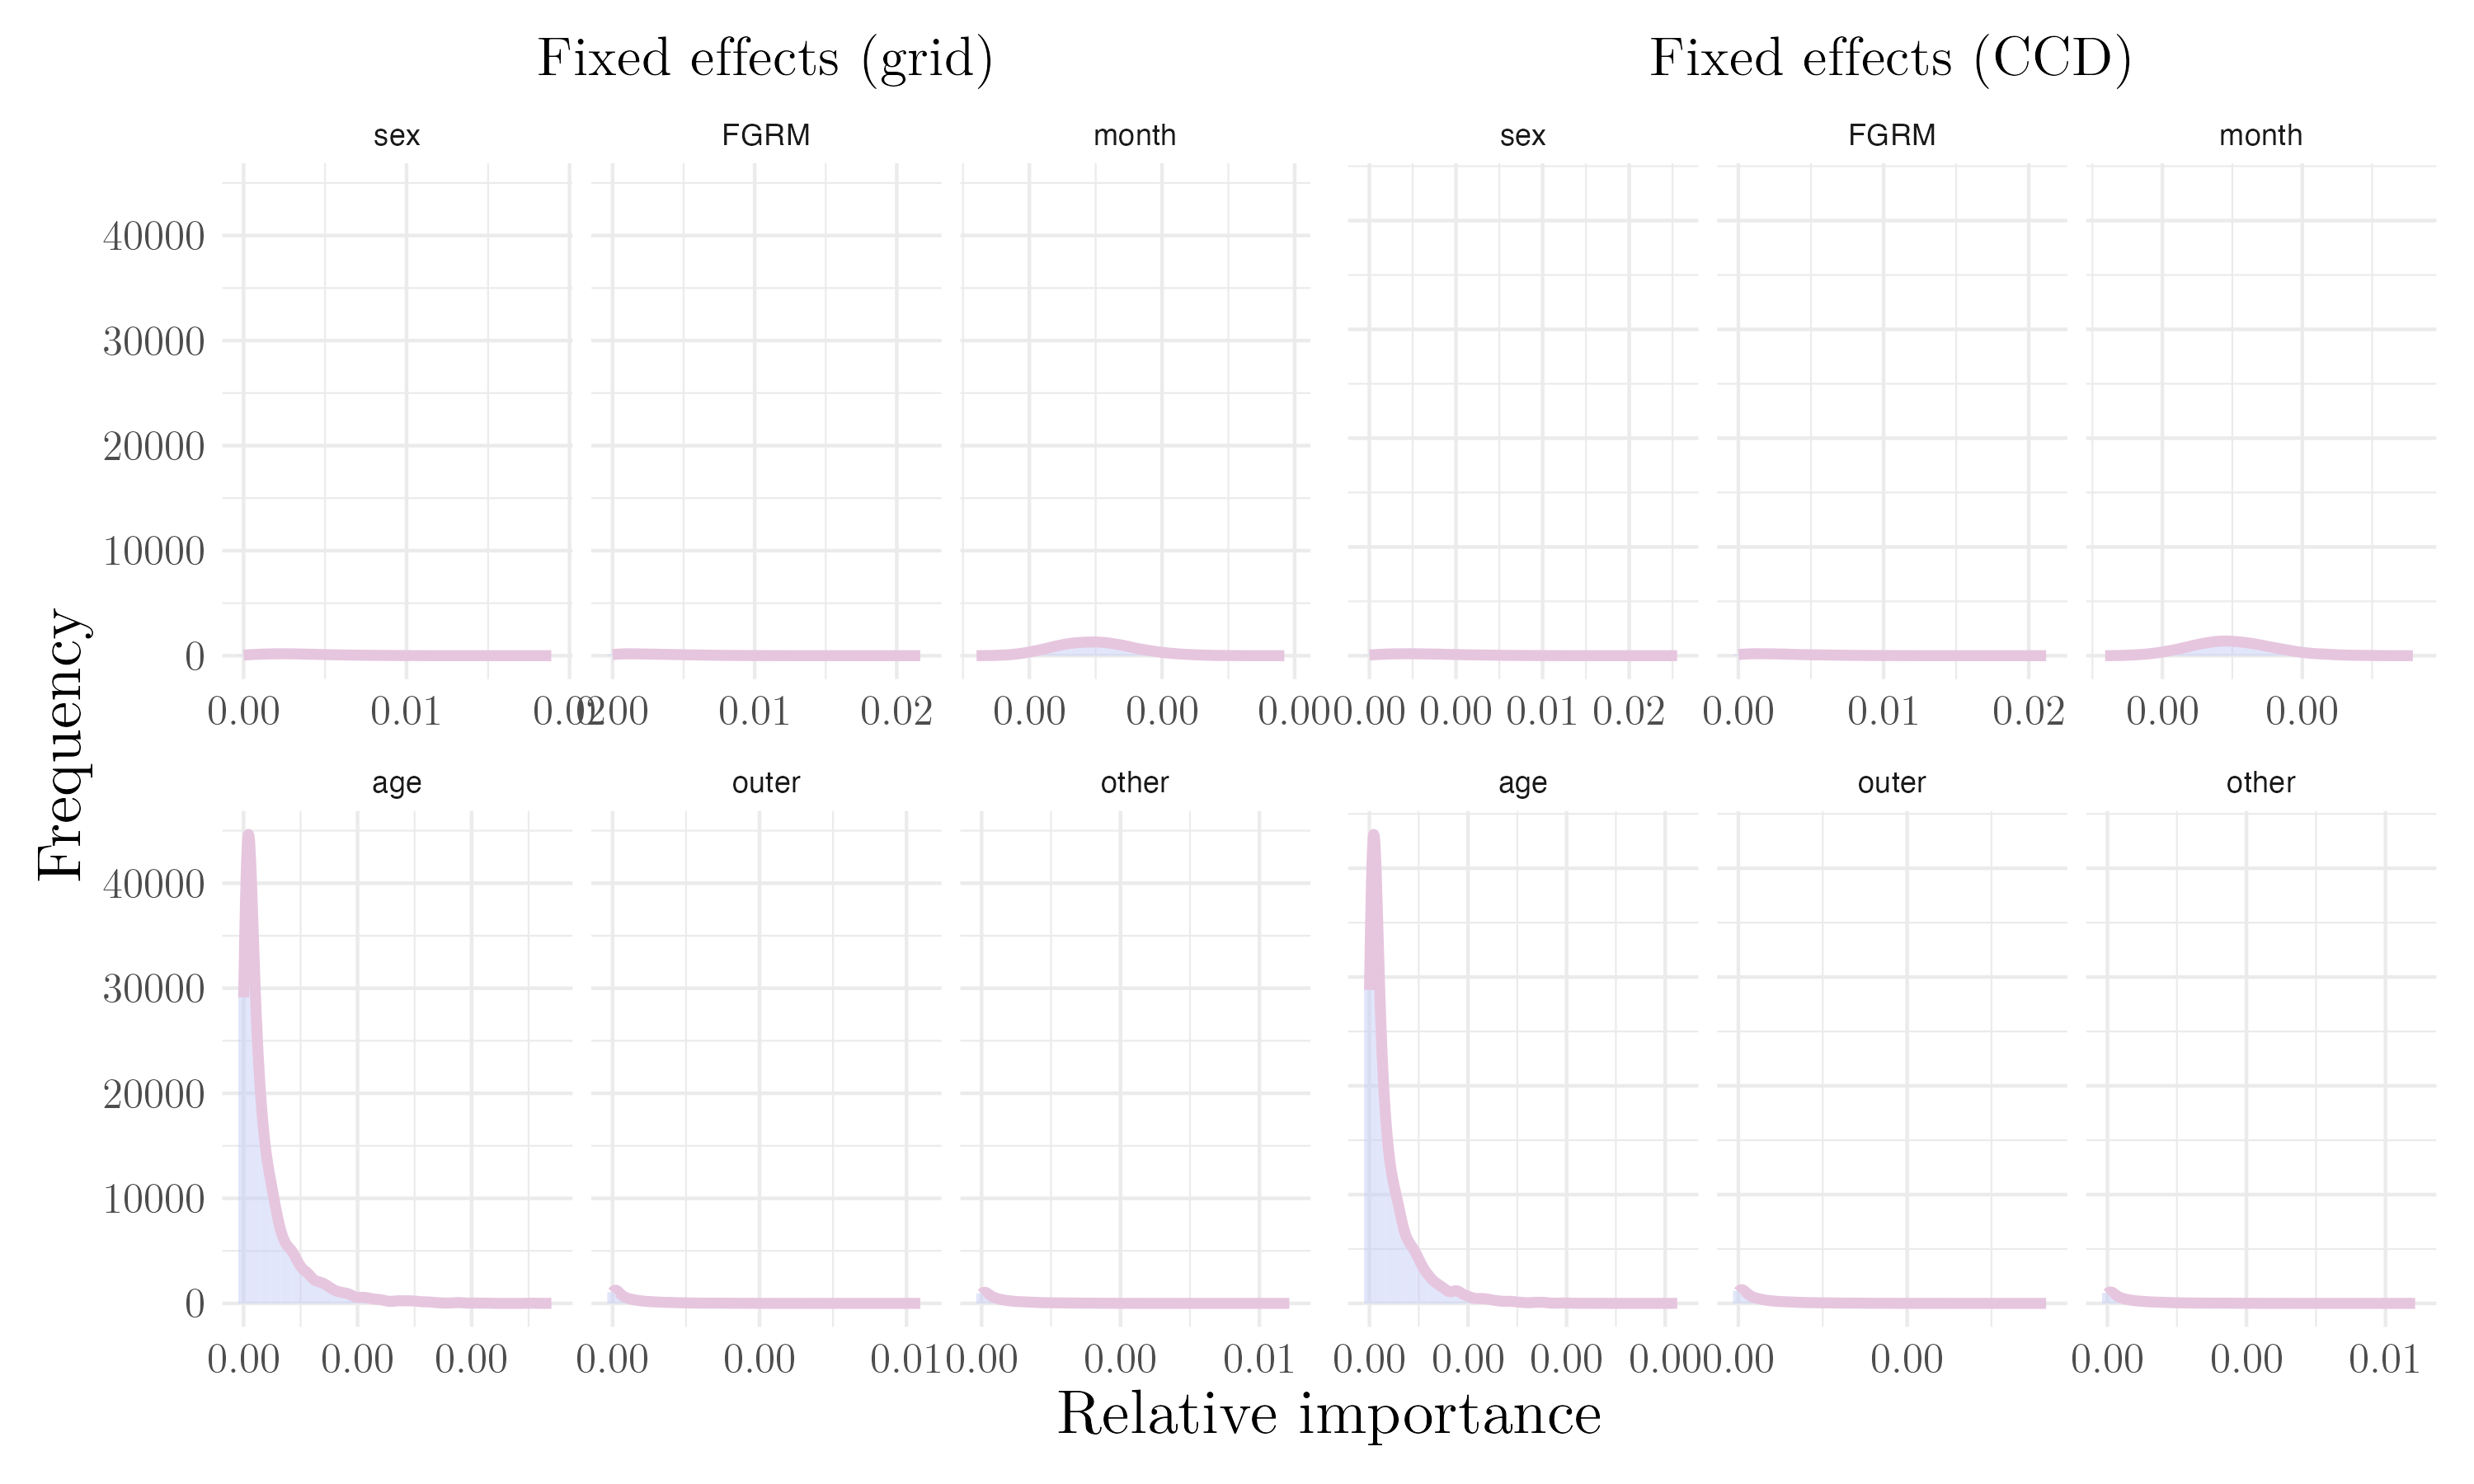
\includegraphics[width=1\linewidth]{Figures/House sparrow study/Tarsus_fixed.png}
%   \caption[Posterior relative importance distributions of all fixed effects in tarsus length model for house sparrow study]{Posterior relative importance distributions of all fixed effects in heritability of tarsus length model for house sparrow study. The grid integration is displayed on the left, and CCD on the right.}
%   \label{fig:tarsus_fixed_sparrows}
% \end{figure}
% In the random effects of the tarsus length model (\Cref{fig:tarsus_random_sparrows}), the Gaussian observations receive the smallest share of importance, while the overdispersive term \textit{IDC} is assigned the largest share. It also seems that the spread of posterior importance distributions for \textit{IDC} and \textit{IDC2} are quite large in this case. As for body mass and wing length, the \textit{hatchyear} covariate is given a small share. The integration strategies agree for the most part, but the grid integration show signs of a trimodal pattern for \textit{IDC} and \textit{IDC2}, with the latter corresponding to the heritability.
% \begin{figure}[H]%\ContinuedFloat
%   \centering
%   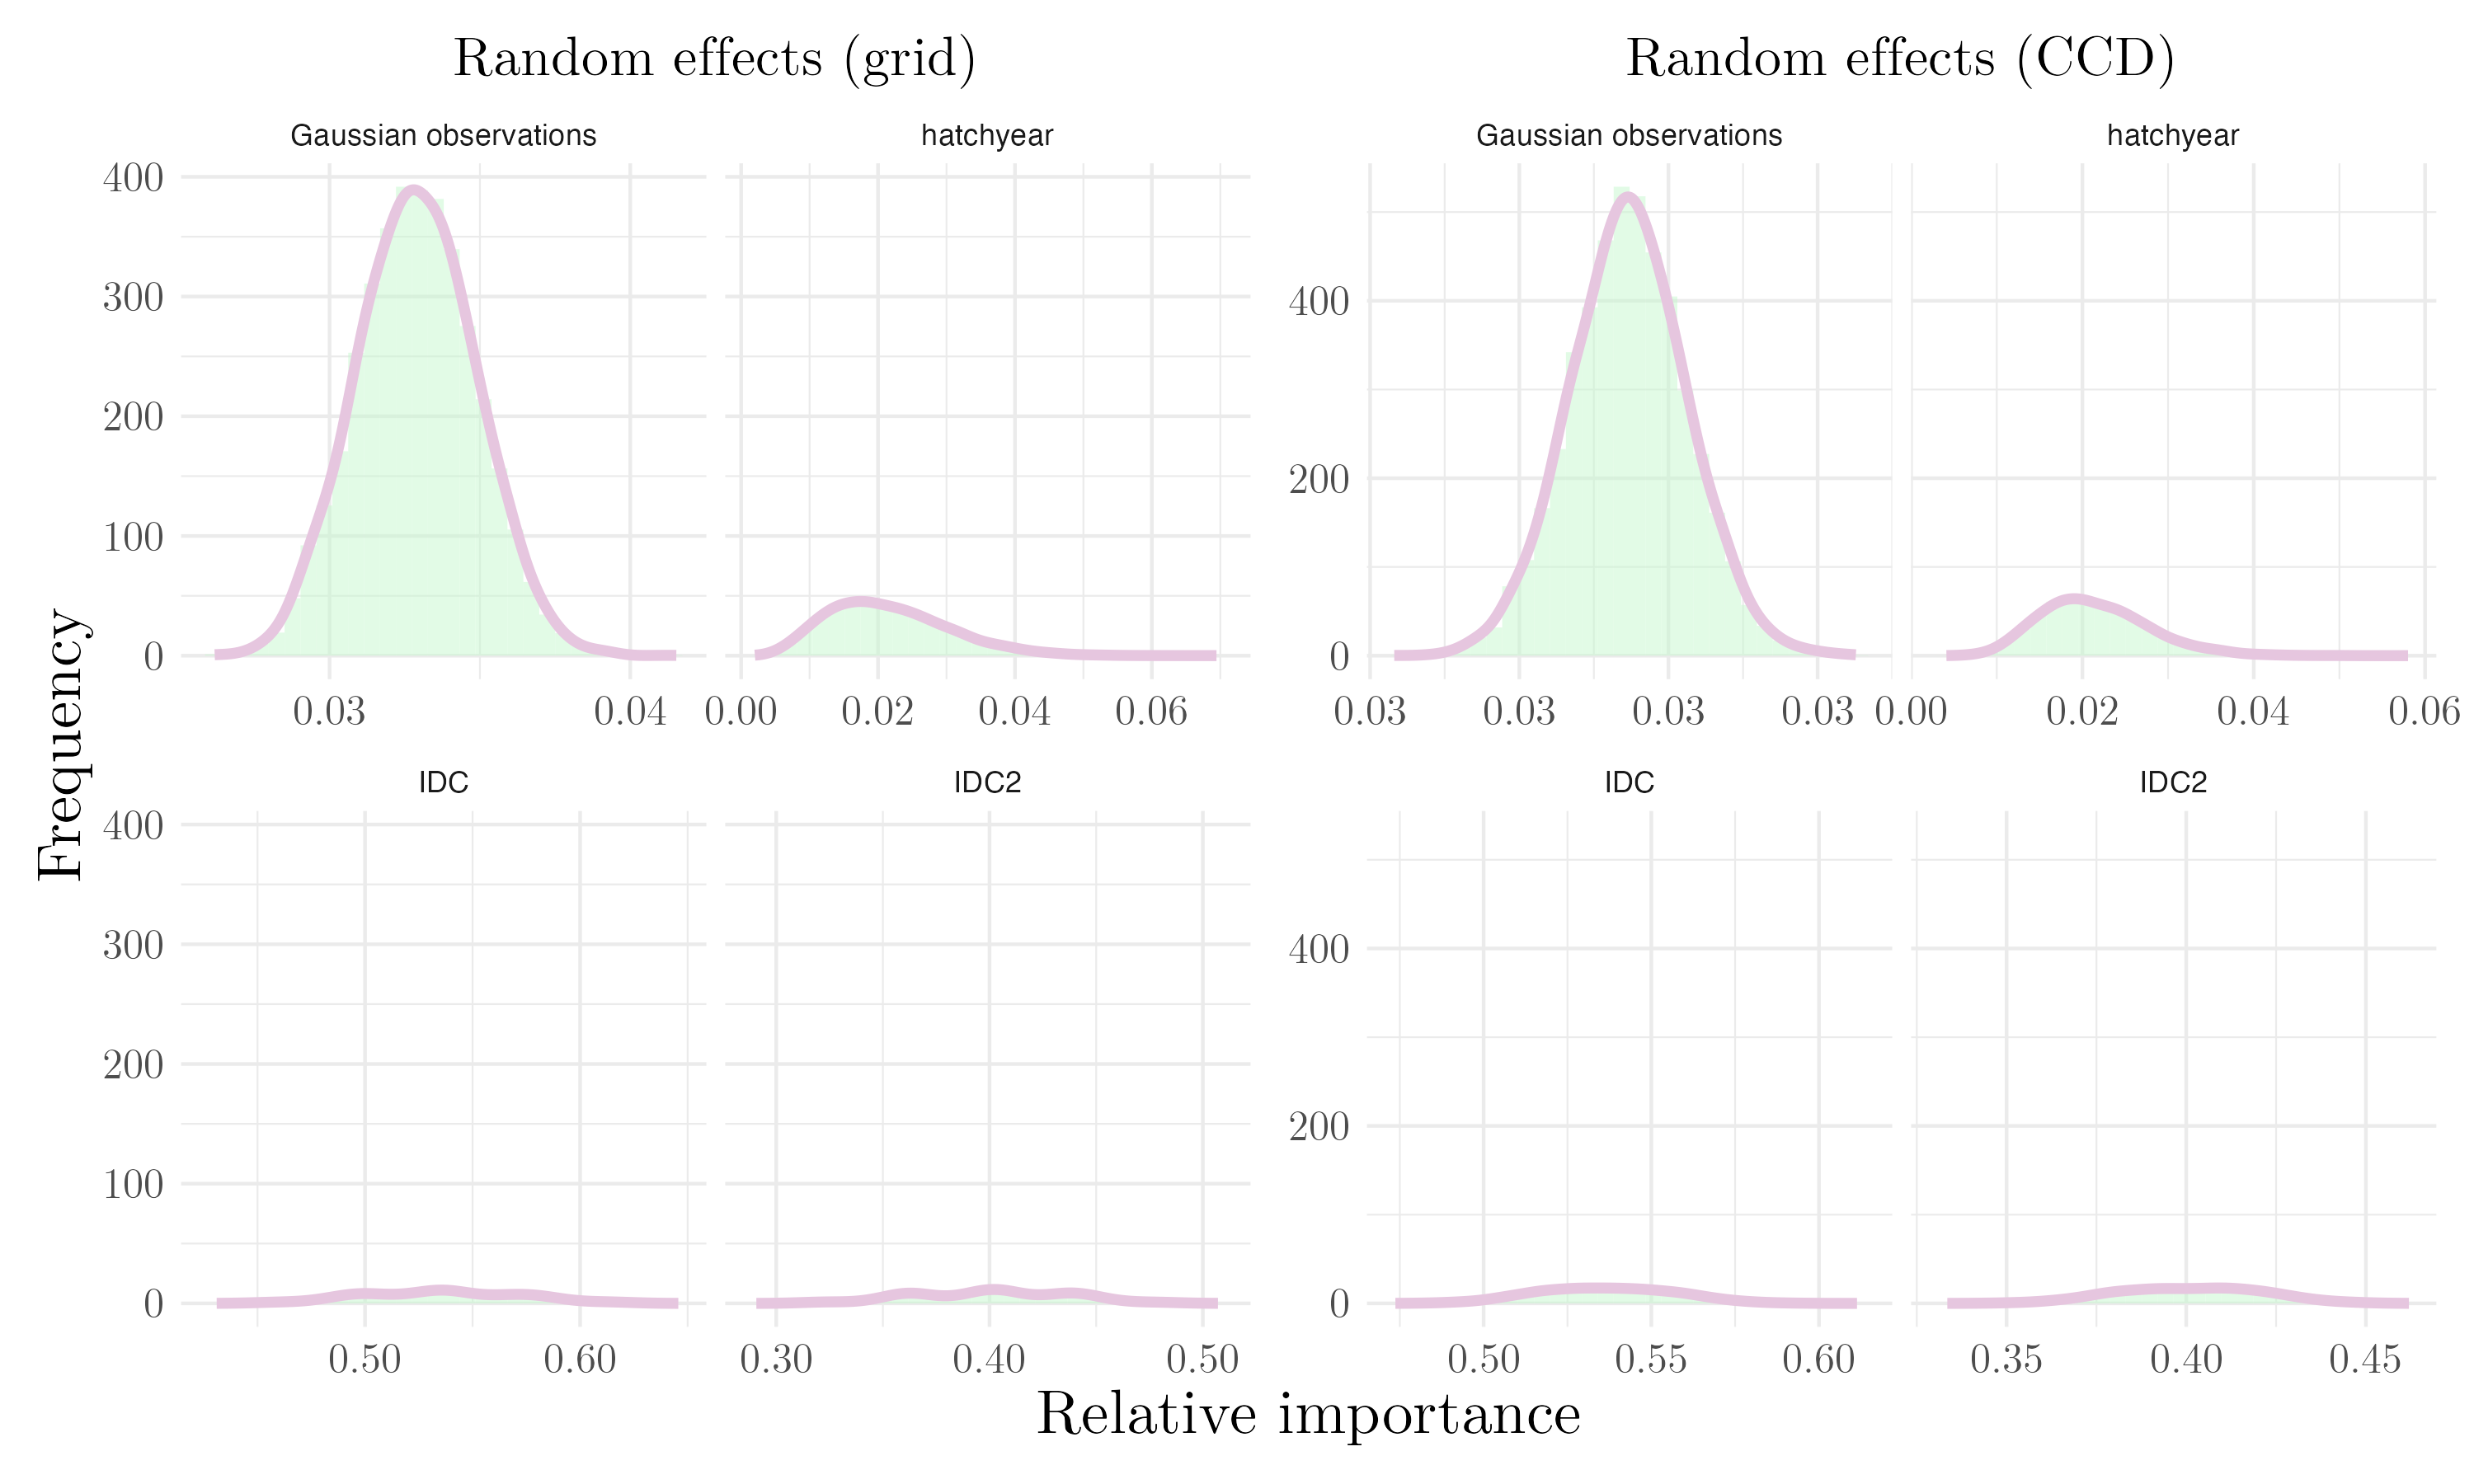
\includegraphics[width=1\linewidth]{Figures/House sparrow study/Tarsus_random.png}
%   \caption[Posterior relative importance distributions of all random effects in tarsus length model for house sparrow study]{Posterior relative importance distributions of all random effects in heritability of tarsus length model for house sparrow study. The grid integration is displayed on the left, and CCD on the right.}
%   \label{fig:tarsus_random_sparrows}
% \end{figure}
% The $R^2$ estimates for the tarsus length model (\Cref{fig:tarsus_r2}) indicate a very small marginal $R^2$, reflecting the minimal importance assigned to the fixed effects. Contrarily, the conditional $R^2$ is extremely high, as the Gaussian observations were given a very small importance. The peaks of the CCD strategy is a bit sharper than that of the grid integration. 
% \begin{figure}[H]%\ContinuedFloat
%   \centering
%   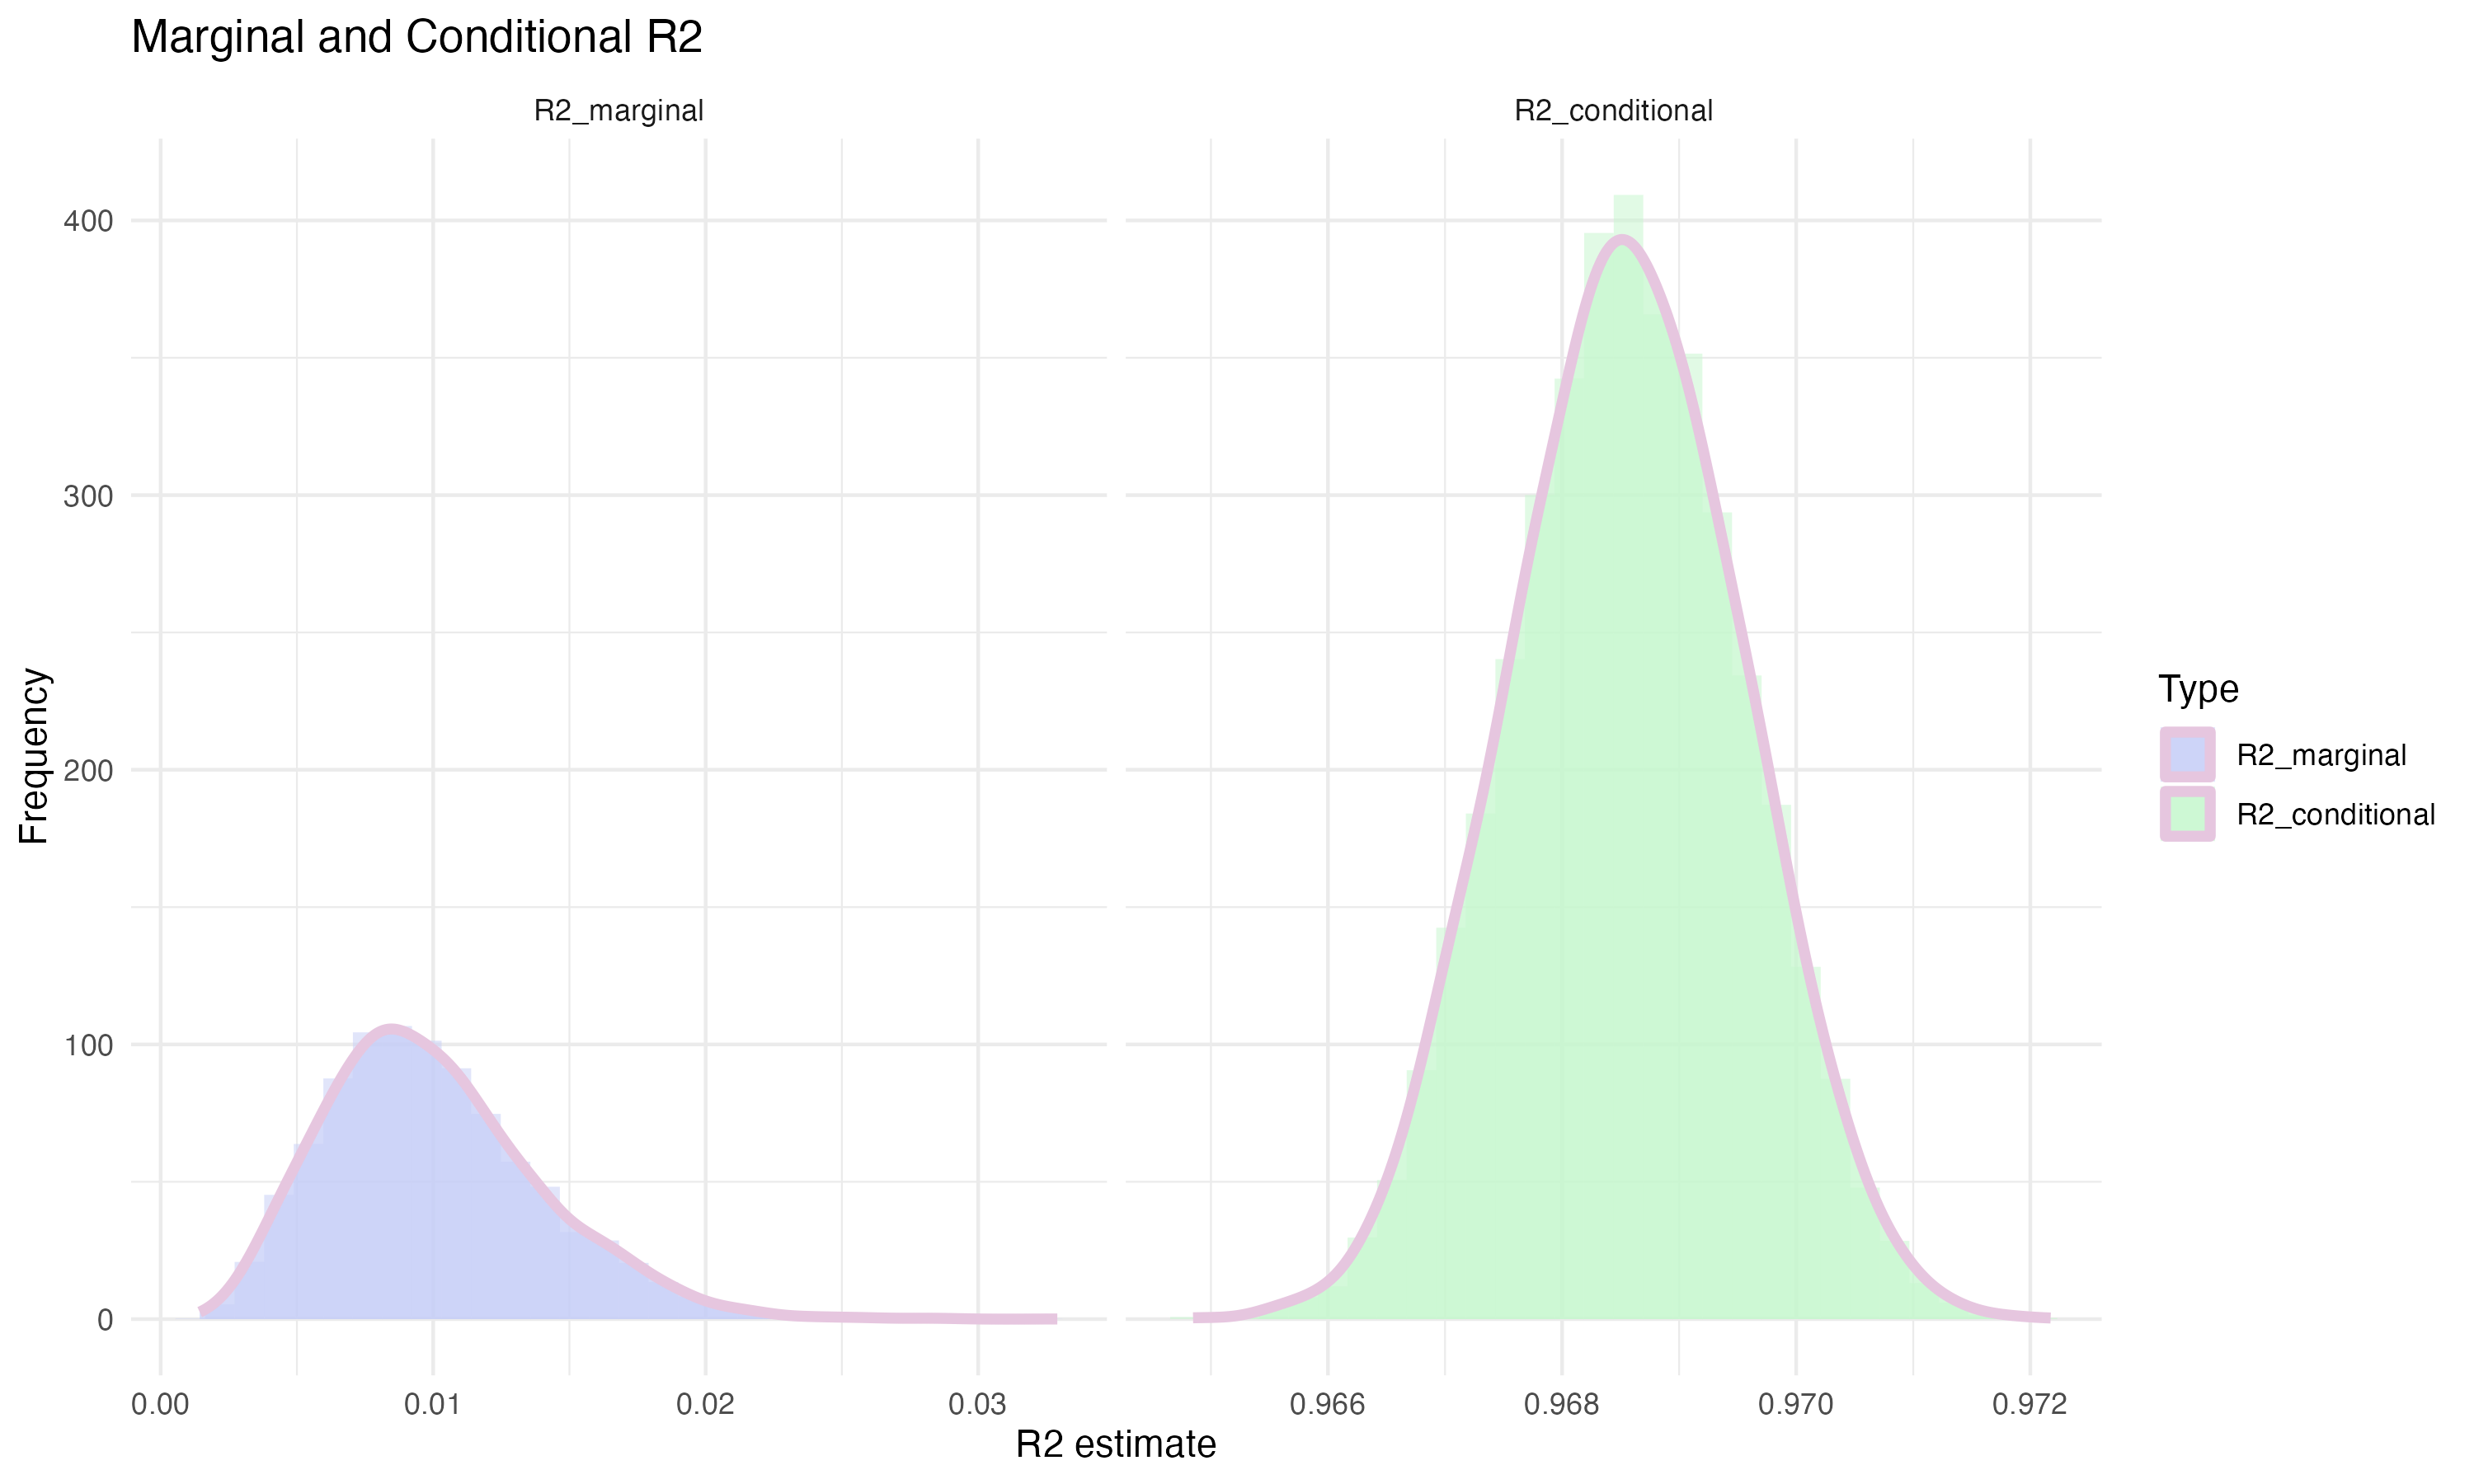
\includegraphics[width=1\linewidth]{Figures/House sparrow study/Tarsus_r2.png}
%   \caption[Posterior distributions of $R^2$ values in tarsus length model for house sparrow study]{Posterior distributions of $R^2$ values in heritability tarsus length model for house sparrow study. The grid integration is displayed on the left, and CCD on the right.}
%   \label{fig:tarsus_r2}
% \end{figure}
\section{Supplementary tables for the non-Gaussian simulation study}
We attach the summarizing tables for the Binomial and Poisson simulation studies here, as they were referred to throughout the thesis. Firstly, \Cref{table:summary_logit} contains summary statistics of the distribution obtained from the Binomial model, while \Cref{table:summary_poisson} contains the same for the Poisson model.
\begin{table}[ht]
    \centering
    \begin{tabular}{@{}llcccccc@{}}
      \toprule
      \multicolumn{2}{c}{\textbf{Measure}} & $\mathbf{\rho=0}$ & $\mathbf{\rho=0.1}$ & $\mathbf{\rho=-0.1}$ & $\mathbf{\rho=0.4}$ & $\mathbf{\rho=-0.4}$ \\ \midrule
      \multirow{3}{*}{\shortstack{Relative Importance of \\ Fixed effect X1}} & Average & 0.098 & 0.118 & 0.077 & 0.173 & 0.020 \\
                                               & 2.5\%   & 0.086 & 0.106 & 0.067 & 0.161 & 0.017 \\
                                               & 97.5\%  & 0.108 & 0.130 & 0.088 & 0.185 & 0.023 \\ \midrule
      \multirow{3}{*}{\shortstack{Relative Importance of \\ Fixed effect X2}} & Average & 0.194 & 0.208 & 0.176 & 0.239 & 0.077 \\
                                               & 2.5\%   & 0.177 & 0.194 & 0.161 & 0.226 & 0.066 \\
                                               & 97.5\%  & 0.210 & 0.223 & 0.193 & 0.251 & 0.087 \\ \midrule
      \multirow{3}{*}{\shortstack{Relative Importance of \\ Fixed effect X3}} & Average & 0.292 & 0.298 & 0.280 & 0.299 & 0.166 \\
                                               & 2.5\%   & 0.272 & 0.280 & 0.258 & 0.285 & 0.150 \\
                                               & 97.5\%  & 0.310 & 0.317 & 0.300 & 0.315 & 0.182 \\ \midrule
      \multirow{3}{*}{\shortstack{Relative Importance of \\ Random effect}} & Average & 0.097 & 0.087 & 0.107 & 0.067 & 0.171 \\
                                               & 2.5\%   & 0.073 & 0.066 & 0.081 & 0.050 & 0.131 \\
                                               & 97.5\%  & 0.121 & 0.117 & 0.139 & 0.086 & 0.211 \\ \midrule
      \multirow{3}{*}{$R^2_m$}            & Average & 0.583 & 0.624 & 0.532 & 0.710 & 0.262 \\
                                           & 2.5\%   & 0.558 & 0.600 & 0.507 & 0.690 & 0.241 \\
                                           & 97.5\%  & 0.607 & 0.646 & 0.557 & 0.730 & 0.284 \\ \midrule
      \multirow{3}{*}{$R^2_c$}            & Average & 0.680 & 0.712 & 0.640 & 0.777 & 0.434 \\
                                           & 2.5\%   & 0.659 & 0.695 & 0.617 & 0.763 & 0.401 \\
                                           & 97.5\%  & 0.700 & 0.731 & 0.660 & 0.792 & 0.468 \\ \bottomrule
    \end{tabular}
    % \begin{tabular}{@{}llcccccc@{}}
    %   \toprule
    %   \multicolumn{2}{c}{\textbf{Measure}} & $\mathbf{\rho=0}$ & $\mathbf{\rho=0.1}$ & $\mathbf{\rho=-0.1}$ & $\mathbf{\rho=0.4}$ & $\mathbf{\rho=-0.4}$ \\ \midrule
    %   \multirow{3}{*}{\shortstack{Relative Importance of \\ Random effect}} & Average & 0.096 & 0.086 & 0.107 & 0.067 & 0.169 \\
    %                                      & 2.5\%   & 0.069 & 0.062 & 0.079 & 0.047 & 0.130 \\
    %                                      & 97.5\%  & 0.126 & 0.112 & 0.139 & 0.089 & 0.219 \\ \midrule
    %   \multirow{3}{*}{\shortstack{Relative Importance of \\ Fixed effect X1}} & Average & 0.097 & 0.117 & 0.077 & 0.173 & 0.020 \\
    %                                        & 2.5\%   & 0.080 & 0.101 & 0.063 & 0.156 & 0.017 \\
    %                                        & 97.5\%  & 0.111 & 0.133 & 0.091 & 0.190 & 0.024 \\ \midrule
    %   \multirow{3}{*}{\shortstack{Relative Importance of \\ Fixed effect X2}} & Average & 0.195 & 0.210 & 0.176 & 0.239 & 0.077 \\
    %                                        & 2.5\%   & 0.174 & 0.188 & 0.156 & 0.222 & 0.064 \\
    %                                        & 97.5\%  & 0.215 & 0.232 & 0.197 & 0.257 & 0.089 \\ \midrule
    %   \multirow{3}{*}{\shortstack{Relative Importance of \\ Fixed effect X3}} & Average & 0.292 & 0.298 & 0.280 & 0.298 & 0.167 \\
    %                                        & 2.5\%   & 0.267 & 0.274 & 0.255 & 0.277 & 0.146 \\
    %                                        & 97.5\%  & 0.318 & 0.321 & 0.307 & 0.318 & 0.187 \\ \midrule
    %   \multirow{3}{*}{$R^2_m$}            & Average & 0.584 & 0.625 & 0.534 & 0.710 & 0.264 \\
    %                                        & 2.5\%   & 0.552 & 0.594 & 0.501 & 0.684 & 0.235 \\
    %                                        & 97.5\%  & 0.614 & 0.654 & 0.565 & 0.732 & 0.290 \\ \midrule
    %   \multirow{3}{*}{$R^2_c$}            & Average & 0.680 & 0.711 & 0.641 & 0.778 & 0.433 \\
    %                                        & 2.5\%   & 0.653 & 0.684 & 0.613 & 0.758 & 0.392 \\
    %                                        & 97.5\%  & 0.705 & 0.735 & 0.668 & 0.797 & 0.477 \\ \bottomrule
    % \end{tabular}
    \caption[Summary statistics for binomial GLMM simulation study]{Summary of simulation study results for the quantiles of relative importance estimates of the Logit model across different correlation levels. For $\rho=0$ the expected values are given in \Cref{table:3}.}
    \label{table:summary_logit}
\end{table}
\begin{table}[ht]
    \centering
    \begin{tabular}{@{}llcccccc@{}}
      \toprule
      \multicolumn{2}{c}{\textbf{Measure}} & $\mathbf{\rho=0}$ & $\mathbf{\rho=0.1}$ & $\mathbf{\rho=-0.1}$ & $\mathbf{\rho=0.4}$ & $\mathbf{\rho=-0.4}$ \\ \midrule
      \multirow{3}{*}{\shortstack{Relative Importance of \\ Fixed effect X1}} & Average & 0.097 & 0.119 & 0.075 & 0.181 & 0.017 \\
                                           & 2.5\%   & 0.088 & 0.109 & 0.066 & 0.172 & 0.015 \\
                                           & 97.5\%  & 0.107 & 0.128 & 0.084 & 0.189 & 0.020 \\ \midrule
      \multirow{3}{*}{\shortstack{Relative Importance of \\ Fixed effect X2}} & Average & 0.193 & 0.212 & 0.171 & 0.251 & 0.066 \\
                                           & 2.5\%   & 0.181 & 0.200 & 0.158 & 0.241 & 0.057 \\
                                           & 97.5\%  & 0.205 & 0.224 & 0.184 & 0.260 & 0.075 \\ \midrule
      \multirow{3}{*}{\shortstack{Relative Importance of \\ Fixed effect X3}} & Average & 0.290 & 0.302 & 0.272 & 0.314 & 0.143 \\
                                           & 2.5\%   & 0.276 & 0.288 & 0.256 & 0.302 & 0.130 \\
                                           & 97.5\%  & 0.307 & 0.316 & 0.289 & 0.326 & 0.156 \\ \midrule
      \multirow{3}{*}{\shortstack{Relative Importance of \\ Random effect}} & Average & 0.098 & 0.090 & 0.106 & 0.072 & 0.149 \\
                                           & 2.5\%   & 0.074 & 0.068 & 0.081 & 0.054 & 0.111 \\
                                           & 97.5\%  & 0.127 & 0.112 & 0.136 & 0.093 & 0.190 \\ \midrule
      \multirow{3}{*}{$R^2_m$}            & Average & 0.580 & 0.633 & 0.519 & 0.746 & 0.225 \\
                                           & 2.5\%   & 0.558 & 0.613 & 0.496 & 0.727 & 0.207 \\
                                           & 97.5\%  & 0.601 & 0.654 & 0.541 & 0.763 & 0.244 \\ \midrule
      \multirow{3}{*}{$R^2_c$}            & Average & 0.679 & 0.723 & 0.625 & 0.817 & 0.374 \\
                                           & 2.5\%   & 0.658 & 0.704 & 0.602 & 0.804 & 0.337 \\
                                           & 97.5\%  & 0.700 & 0.741 & 0.648 & 0.830 & 0.413 \\ \bottomrule
    \end{tabular}
    % \begin{tabular}{@{}llcccccc@{}}
    %   \toprule
    %   \multicolumn{2}{c}{\textbf{Measure}} & $\mathbf{\rho=0}$ & $\mathbf{\rho=0.1}$ & $\mathbf{\rho=-0.1}$ & $\mathbf{\rho=0.4}$ & $\mathbf{\rho=-0.4}$ \\ \midrule
    %   \multirow{3}{*}{\shortstack{Relative Importance of \\ Random effect}} & Average & 0.095 & 0.088 & 0.104 & 0.072 & 0.147 \\
    %                                      & 2.5\%   & 0.070 & 0.066 & 0.073 & 0.053 & 0.107 \\
    %                                      & 97.5\%  & 0.124 & 0.117 & 0.137 & 0.093 & 0.194 \\ \midrule
    %   \multirow{3}{*}{\shortstack{Relative Importance of \\ Fixed effect X1}} & Average & 0.097 & 0.119 & 0.075 & 0.181 & 0.017 \\
    %                                        & 2.5\%   & 0.085 & 0.106 & 0.064 & 0.171 & 0.014 \\
    %                                        & 97.5\%  & 0.108 & 0.131 & 0.086 & 0.192 & 0.021 \\ \midrule
    %   \multirow{3}{*}{\shortstack{Relative Importance of \\ Fixed effect X2}} & Average & 0.194 & 0.213 & 0.171 & 0.251 & 0.066 \\
    %                                        & 2.5\%   & 0.180 & 0.199 & 0.155 & 0.240 & 0.054 \\
    %                                        & 97.5\%  & 0.210 & 0.229 & 0.187 & 0.263 & 0.079 \\ \midrule
    %   \multirow{3}{*}{\shortstack{Relative Importance of \\ Fixed effect X3}} & Average & 0.292 & 0.303 & 0.273 & 0.313 & 0.142 \\
    %                                        & 2.5\%   & 0.2725 & 0.2848 & 0.2522 & 0.2994 & 0.124 \\
    %                                        & 97.5\%  & 0.3102 & 0.3213 & 0.2925 & 0.3258 & 0.162 \\ \midrule
    %   \multirow{3}{*}{$R^2_m$}            & Average & 0.5827 & 0.6343 & 0.519 & 0.746 & 0.225 \\
    %                                        & 2.5\%   & 0.557 & 0.610 & 0.494 & 0.726 & 0.201 \\
    %                                        & 97.5\%  & 0.606 & 0.657 & 0.541 & 0.765 & 0.250 \\ \midrule
    %   \multirow{3}{*}{$R^2_c$}            & Average & 0.678 & 0.723 & 0.623 & 0.818 & 0.371 \\
    %                                        & 2.5\%   & 0.656 & 0.702 & 0.595 & 0.803 & 0.335 \\
    %                                        & 97.5\%  & 0.700 & 0.743 & 0.648 & 0.832 & 0.414 \\ \bottomrule
    % \end{tabular}
    \caption[Summary statistics for Poisson GLMM simulation study]{Summary of simulation study results for the quantiles of relative importance estimates the Poisson model across different correlation levels. For $\rho=0$ the expected values are given in \Cref{table:3}.}
    \label{table:summary_poisson}
  \end{table}

\chapter{Miscellaneous proofs}
\label{ap:proofs}
We present a joint proof of the expectation and variance of a random variable belonging to the univariate exponential family.
For a random variable $Y$ with a normalized probability density function $f(y \lvert \theta, \phi)$ on the form
\begin{equation}
    f(y \lvert \theta, \phi) = \exp\left( \frac{y\theta - b(\theta)}{a(\phi)} + c(y, \phi) \right) \ ,
\end{equation}
where $\theta$ is the natural parameter and $\phi$ is the dispersion parameter, the expectation and variance of $Y$ can be expressed as
\begin{equation}
    \begin{aligned}
        \mathbb{E}(Y \lvert \theta) &= b'(\theta) \\
        \text{Var}(Y \lvert \theta) &= b''(\theta)
    \end{aligned}
\end{equation}
This can be proven by considering the following:
\begin{equation}
    \frac{d f(y)}{d\theta} = \frac{1}{a(\phi)} f(y \lvert \theta, \phi) (y-b'(\theta))  \ ,
\end{equation}
and 
\begin{equation}
    \frac{d^2 f(y)}{d\theta^2} = \frac{1}{a(\phi)}f(y \lvert \theta, \phi) \left( \frac{1}{a(\phi)}(y-b'(\theta))^2 - b''(\theta) \right) \ .
\end{equation}
Now, assuming mild regularity to interchange derivation and integration and noting that  $\int_{\mathbb{R}} f(y \lvert \theta) dy = 1$, we have 
\begin{equation}
    \label{eq:expfam_expectation}
    \frac{d}{d \theta} \int_{\mathbb{R}} f(y) dy  = \int_{\mathbb{R}} \frac{d f}{d\theta} dy = 0 \ ,
\end{equation}
and 
\begin{equation}
    \label{eq:expfam_variance}
    \frac{d^2}{d \theta^2} \int_{\mathbb{R}} f(y) dy = \int_{\mathbb{R}} \frac{d^2 f}{d\theta^2} dy = 0 \ .
\end{equation}
Equations \eqref{eq:expfam_expectation} and \eqref{eq:expfam_variance} can be used to derive the relation 
\begin{equation}
    \begin{aligned}
    0 = \int_{\mathbb{R}} \frac{d f(y)}{d\theta} dy &= \frac{1}{a(\phi)}\int_{\mathbb{R}} f(y) (y-b'(\theta)) dy \\
    & = \frac{1}{a(\phi)} \left(\mathbb{E}(Y \lvert \theta) - b'(\theta)\int_{\mathbb{R}}f(y)dy \right) \\
    & = \frac{1}{a(\phi)} \left( \mathbb{E}(Y \lvert \theta) - b'(\theta) \right) \\
    & \implies \mathbb{E}(Y \lvert \theta) = b'(\theta) \ ,
    \end{aligned}
\end{equation}
and 
\begin{equation}
    \begin{aligned}
    0 = \int_{\mathbb{R}} \frac{d^2 f(y)}{d\theta^2} dy &= \frac{1}{a(\phi)} \int_{\mathbb{R}} f(y) \left( \frac{1}{a(\phi)}(y-b'(\theta))^2 - b''(\theta) \right) dy \\
    &= \frac{1}{a(\phi)} \int_{\mathbb{R}} f(y) \left( \frac{1}{a(\phi)} (y-\mathbb{E}(Y))^2 - b''(\theta) \right) dy \\
    &= \frac{1}{ a(\phi)} \left( \mathbb{E}[(y-\mathbb{E}(Y))^2]- b''(\theta) \int_{\mathbb{R}} f(y)dy \right) \\
    & = \frac{1}{a(\phi)}\text{Var}(Y) - b''(\theta) \\
    & \implies \text{Var}(Y \lvert \theta) = a(\phi) b''(\theta) \ \qedsymbol
    \end{aligned}
\end{equation}

% \chapter*{\LARGE \textbf{Appendices}}
% \fancyhf{} %clear the header, it should be empty for the appendices
% \renewcommand{\headrulewidth}{0pt} %no rule
% \fancyfoot[C]{\thepage} %set the page numbers in the center of the footer instead 

% %it is possible to set a different page numbering style for the appendix, but I personally just continued with the same page numbering as the main content as I find that more tidy
% %\pagenumbering{roman}
% %\setcounter{page}{1}
% \addcontentsline{toc}{chapter}{\protect\numberline{}Appendices:}
% \appendix
% \label{ap:appendix}
% \input{Chapters/08Appendix}


\end{document}
